\documentclass[a4paper]{report}
\usepackage{vntex}
\usepackage[fontsize=12pt]{scrextend}
\usepackage{mathptmx}[ptm]
%\usepackage[utf8]{inputenc}
% \usepackage[english, vietnamese]{babel}
\usepackage{csquotes}
\usepackage{amssymb,epsfig,latexsym,array,hhline,fancyhdr}
\usepackage[normalem]{ulem}
\usepackage{titlesec}

%\usepackage{soul}
\usepackage[makeroom]{cancel}
\usepackage{amsmath}
\usepackage{amsthm}
\usepackage{multicol,longtable,amscd}
\usepackage{diagbox}%Make diagonal lines in tables
\usepackage{booktabs}
\usepackage{alltt}
\usepackage[framemethod=tikz]{mdframed}% For highlighting paragraph backgrounds
\usepackage{caption,subcaption}
\captionsetup{skip=16pt} % Increase space between figure and caption globally

\usepackage[lined,boxed,commentsnumbered]{algorithm2e}
\usepackage{enumerate}
\usepackage{color}
\usepackage{graphicx}							% Standard graphics package
\usepackage{array}
\usepackage{tabularx, caption}
\usepackage{xltabular}
\usepackage{ragged2e}
\usepackage{fontawesome5}
\usepackage{multirow}
\usepackage{multicol}
\usepackage{rotating}
\usepackage{graphics}
\usepackage{geometry}
\usepackage{setspace}
\usepackage{epsfig}
\usepackage{tikz}
\usepackage{longfbox}

\usetikzlibrary{arrows,snakes,backgrounds,calc}
\usepackage[unicode]{hyperref}
\hypersetup{urlcolor=blue,linkcolor=black,citecolor=black,colorlinks=true} 
\usepackage{listings}
\usepackage{float}
\usepackage{pdflscape}
\usepackage{pdfpages}
\usepackage[export]{adjustbox} % Cho phép ảnh tự cắt khi hết trang
\usepackage{tocloft}

\usepackage{appendix}
% algorithm2e configuration (replacing algorithm/algorithmic)
\SetKwInput{Input}{Input:}
\SetKwInput{Output}{Output:}
%\usepackage{pstcol} 								% PSTricks with the standard color package
\usepackage{enumitem} % Put this in the preamble
\usepackage[normalem]{ulem}
\usepackage{lastpage}   % Load this LAST

\newcommand{\autofitgraphics}[2][]{\includegraphics[#1]{#2}}

\renewcommand{\bibname}{Tài liệu tham khảo}

\newtheorem{theorem}{{\bf Định lý}}
\newtheorem{property}{{\bf Tính chất}}
\newtheorem{proposition}{{\bf Mệnh đề}}
\newtheorem{corollary}[proposition]{{\bf Hệ quả}}
\newtheorem{lemma}[proposition]{{\bf Bổ đề}}
\theoremstyle{definition}
\newtheorem{exer}{Bài toán}
% Định nghĩa một kiểu cột X mới (L), căn lề trái (thay vì dàn đều hai bên)
% Giúp văn bản trong các ô dài dễ đọc hơn.
\newcolumntype{L}{>{\RaggedRight\arraybackslash}X}
% \addtocontents{toc}{\protect\thispagestyle{empty}}
% Remove page number in contents page. 
% \addtocontents{lof}{\protect\thispagestyle{empty}}
% Remove page number in list of figure page. 
% \addtocontents{lot}{\protect\thispagestyle{empty}}
% Remove page number in list of table page. 
% \def\thesislayout{	% A4: 210 × 297
% 	\geometry{
% 		a4paper,
% 		total={160mm,240mm},  % fix over page
% 		left=30mm,
% 		top=22mm,
%             right=20mm,
%             bottom=20mm,
% 	}
% }
% \def\thesisheadlayout{	% A4: 210 × 297
% 	\geometry{
% 		a4paper,
% 		total={160mm,240mm},  % fix over page
% 		left=30mm,
% 		top=10mm,
% 	}
% }
\def\thesislayout{	% A4: 210 × 297
	\geometry{
		a4paper,
		total={210mm,297mm},  % fix over page
		left=35mm,
		top=25mm,
            bottom=30mm,
            right=30mm
	}
}
\def\thesisheadlayout{	% A4: 210 × 297
	\geometry{
		a4paper,
		total={210mm,297mm},  % fix over page
		left=40mm,
		top=30mm,
            bottom=30mm,
            right=30mm
	}
}
\thesislayout
\lstset{
language=R,
basicstyle=\footnotesize\sffamily,
commentstyle=\ttfamily\color{black},
numbers=left,
numberstyle=\ttfamily\color{black}\footnotesize,
stepnumber=1,
numbersep=5pt,
backgroundcolor=\color{white},
showspaces=false,
showstringspaces=false,
showtabs=false,
frame=single,
tabsize=2,
captionpos=b,
breaklines=true,
breakatwhitespace=false,
title=\lstname,
escapeinside={},
keywordstyle={},
morekeywords={}
}
%\usepackage{fancyhdr}
\setlength{\headheight}{40pt}
\pagestyle{fancy}
\fancyhead{} % clear all header fields
\renewcommand{\footruleskip}{1mm}

\fancyhead[L]{
 \begin{tabular}{rl}
    \begin{picture}(25,15)(0,0)
    \put(0,-8){
\includegraphics[width=10mm, height=10mm]{Images/hcmut.png}}
    %\put(0,-8){
\epsfig{width=10mm,figure=hcmut.eps}}
   \end{picture}&
	%
\includegraphics[width=8mm, height=8mm]{hcmut.png} & %
	\begin{tabular}{l}
		\textbf{  Trường Đại Học Bách Khoa - Đại học Quốc gia TP.HCM }\\
		\textbf{  Khoa Khoa Học \& Kỹ Thuật Máy Tính}
	\end{tabular} 	
 \end{tabular}
}
\fancyhead[R]{
	\begin{tabular}{l}
		\tiny \bf \\
		\tiny \bf 
	\end{tabular}  }
\fancyfoot{} % clear all footer fields
\fancyfoot[L]{\scriptsize  Báo cáo Đồ án tốt nghiệp (CO4337) - HK2 2025 - 2026}
\fancyfoot[R]{\scriptsize  Trang {\thepage}/\pageref{LastPage}}

\renewcommand{\headrulewidth}{0.3pt}
\renewcommand{\footrulewidth}{0.3pt}
% Apply the same footer to the plain page style (used by chapters)
% (Moved to end of preamble)
\setlength\parindent{0pt}
%%%
\setcounter{secnumdepth}{4}
\setcounter{tocdepth}{3}
\makeatletter
\newcounter {subsubsubsection}[subsubsection]
\renewcommand\thesubsubsubsection{\thesubsubsection .\@alph\c@subsubsubsection}
\newcommand\subsubsubsection{\@startsection{subsubsubsection}{4}{\z@}%
                                     {-3.25ex\@plus -1ex \@minus -.2ex}%
                                     {1.5ex \@plus .2ex}%
                                     {\normalfont\normalsize\bfseries}}
\newcommand*\l@subsubsubsection{\@dottedtocline{3}{10.0em}{4.1em}}
\newcommand*{\subsubsubsectionmark}[1]{}
\@addtoreset{paragraph}{subsubsection}
\renewcommand\theparagraph{\arabic{paragraph}}
\makeatother
\newcommand\tab[1][1cm]{\hspace*{#1}}
\newcommand\blank[1]{\rule[-.2ex]{#1}{.4pt}}
\everymath{\color{black}}%make in-line maths symbols blue to read/check easily

\sloppy
\captionsetup[figure]{labelfont={small,bf},textfont={small,it},belowskip=0pt,aboveskip=-5pt}
%space remove between caption, figure, and text
\captionsetup[table]{labelfont={small,bf},textfont={small,it},belowskip=-1pt,aboveskip=7pt}
\setlength{\floatsep}{5pt plus 2pt minus 2pt}
\setlength{\textfloatsep}{5pt plus 2pt minus 2pt}
\setlength{\intextsep}{10pt plus 2pt minus 2pt}

\titleformat{\chapter}[display]
{\normalfont\huge\bfseries}{\chaptertitlename{} \thechapter}{15pt}{\Huge}

% Number paragraph headings in a local simple format (1,2,3,...) and avoid run-in sticking.
\titleformat{\paragraph}[block]
{\normalfont\normalsize\bfseries}{\theparagraph.}{0.6em}{}
\titlespacing*{\paragraph}{0pt}{1.2ex plus .2ex minus .1ex}{0.6ex}

\titleformat{\subparagraph}[runin]
{\normalfont\normalsize\bfseries}{}{0pt}{}[\ ]
\titlespacing*{\subparagraph}{0pt}{1ex plus .2ex minus .1ex}{1em}

\thesislayout

% Redefine plain style for chapters and lists to have the footer
\fancypagestyle{plain}{%
  \fancyhf{}%
  \fancyfoot[L]{\scriptsize  Báo cáo Đồ án tốt nghiệp (CO4337) - HK2 2025 - 2026}
  \fancyfoot[R]{\scriptsize  Trang {\thepage}/\pageref{LastPage}}
  \renewcommand{\headrulewidth}{0pt}
  \renewcommand{\footrulewidth}{0.3pt}
}

\begin{document}
\pagenumbering{Roman}

\begin{titlepage}
\begin{tikzpicture}[remember picture, overlay]
  \draw[line width = 4pt] ($(current page.north west) + (0.4in,-0.5in)$) rectangle ($(current page.south east) + (-0.4in,0.5in)$);
  \draw[line width=1.5pt]
    ($ (current page.north west) + (0.45in,-0.55in) $)
    rectangle
    ($ (current page.south east) + (-0.45in,0.55in) $);
\end{tikzpicture}

\vspace*{0.4cm}
\begin{center}
\LARGE \textbf{ĐẠI HỌC QUỐC GIA THÀNH PHỐ HỒ CHÍ MINH} \\[0.25cm]
\LARGE \textbf{TRƯỜNG ĐẠI HỌC BÁCH KHOA} \\[0.25cm]
\LARGE \textbf{KHOA KHOA HỌC VÀ KỸ THUẬT MÁY TÍNH}

\vspace{0.35cm}

\includegraphics[width=3.5cm]{Images/hcmut.png}

\vspace{0.4cm}
\textbf{\LARGE BÁO CÁO}\\[0.2cm]
\textbf{\LARGE ĐỒ ÁN TỐT NGHIỆP}\\[0.2cm]
\textbf{\LARGE NGÀNH KHOA HỌC MÁY TÍNH}

\vspace{1cm}
\textbf{\LARGE Xây dựng Ứng dụng Di động Tư vấn}\\
\textbf{\LARGE Và Đặt lịch Chăm sóc Sức khỏe Ứng dụng Chatbot AI}
\end{center}

\vfill

\begin{center}
\begin{tabular}{r@{\hspace{1.5cm}}l}
\textbf{\Large HỘI ĐỒNG:} & {\Large Hội đồng 11L Khoa học Máy tính}\\[0.22cm]
\textbf{\Large GVHD:} & {\Large TS. Trương Tuấn Anh}\\
 & {\Large CN. Dương Huỳnh Anh Đức}\\[0.22cm]
\textbf{\Large CTHĐ:} & {\Large TS. Nguyễn Thị Ái Thảo}\\[0.22cm]
\textbf{\Large TKHĐ:} & {\Large CN. Dương Huỳnh Anh Đức}\\[0.22cm]
\textbf{\Large UV:} & {\Large ThS. Trần Thị Quế Nguyệt}\\[0.35cm]
\multicolumn{2}{c}{\textbf{\Large ---o0o---}}\\[0.35cm]
\textbf{\Large SVTH1:} & {\Large Lê Nguyễn Gia Hưng - 2211363}\\[0.22cm]
\textbf{\Large SVTH2:} & {\Large Nguyễn Tiến Phát - 1712572}\\[0.22cm]
\textbf{\Large SVTH3:} & {\Large Nguyễn Gia Nguyên - 2212303}
\end{tabular}
\end{center}

\vfill

\begin{center}
{\Large TP. HỒ CHÍ MINH, 6/26}
\end{center}
\vspace*{0.6cm}
\end{titlepage}
\setcounter{page}{2}
%\thispagestyle{empty}
\newpage
%%%%%%%%%%%%%%%%%INTRO%%%%%%%%%%%%%%%%%%%
\section*{Lời cam đoan}
% \thispagestyle{empty}

\hspace*{0.63cm}Tôi xin cam đoan rằng các kết quả, kiến thức được tôi trình bày trong đồ án này hoàn toàn là công sức, nỗ lực của chính nhóm chúng tôi dưới sự dẫn dắt của thầy TS. Trương Tuấn Anh và thầy CN. Dương Huỳnh Anh Đức. Những tài liệu, kiến thức, công trình được nhóm chúng tôi đề cập trong bài báo cáo này đều được trích dẫn rõ ràng, đầy đủ và được liệt kê chi tiết ở phần tài liệu tham khảo.

\hspace*{0.63cm}Tôi xin cam đoan, chấp nhận chịu mọi trách nhiệm nếu nghiên cứu của chúng tôi bị phát hiện có đoạn văn hay bất cứ hành vi vi phạm nào về bản quyền trong nghiên cứu.
\clearpage
% \pagenumbering{arabic}

\section*{Lời cảm ơn}
% \thispagestyle{empty}

\hspace*{0.63cm}Tôi xin được phép gửi lời cảm ơn sâu sắc đến thầy TS. Trương Tuấn Anh và thầy Dương Huỳnh Anh Đức, giảng viên đã trực tiếp hướng dẫn nhóm chúng tôi trong suốt quá trình thực hiện đồ án lần này. Nhờ sự chỉ bảo tận tâm, nhiệt tình của các thầy mà tôi đã đúc kết được những kiến thức, kinh nghiệm quý giá để trau dồi, phát triển bản thân cũng như củng cố lại kiến thức nền tảng để chúng tôi có thể phát triển hơn sau này. Đồ án này chính là một bước ngoặt quan trọng, đánh dấu cho quá trình học tập và trưởng thành tại Trường Đại học Bách Khoa TP HCM.

\hspace*{0.63cm}Lời cảm ơn thứ hai tôi xin dành đến các thầy, cô mà chúng tôi được gặp trong suốt khoảng thời gian học tập tại Trường Đại học Bách Khoa TP HCM. Cảm ơn các thầy, cô giáo Khoa Khoa học và Kỹ thuật Máy tính đã truyền đạt cho chúng tôi những kiến thức chuyên ngành quan trọng để có thể đứng vững và phát triển trong ngành máy tính hiện nay. Và lời cảm ơn cuối cùng, tôi xin dành cho gia đình và bạn bè của tôi, những người luôn hỗ trợ và động viên chúng tôi hết mình trong suốt chặng đường tại Trường Đại học Bách Khoa TP.HCM.

\clearpage
% \pagenumbering{arabic}


\section*{Tóm tắt}
% \thispagestyle{empty}

\hspace*{0.63cm}Đồ án này trình bày việc xây dựng và triển khai nền tảng di động toàn diện HEALYTICS, tập trung vào số hóa quy trình tư vấn và đặt lịch các dịch vụ chăm sóc sức khỏe và sắc đẹp (Wellness). Mục tiêu cốt lõi là giải quyết các thách thức phổ biến như tình trạng người dùng quá tải thông tin và quy trình thủ công, đồng thời cung cấp công cụ để các nhà cung cấp dịch vụ tối ưu hóa quản lý và vận hành.

\hspace*{0.63cm}Giải pháp trung tâm của hệ thống là tích hợp Trí tuệ Nhân tạo (AI). AI được sử dụng để cung cấp chức năng tư vấn thông minh, phân tích nhu cầu tự nhiên của người dùng để đưa ra các gợi ý dịch vụ được cá nhân hóa, phù hợp nhất với hồ sơ sức khỏe của họ. Nền tảng được thiết kế với kiến trúc tổng thể, vững chắc để đảm bảo khả năng mở rộng và độ sẵn sàng cao, bao gồm Ứng dụng Người dùng, Cổng thông tin dành cho Đối tác để quản lý dịch vụ và lịch hẹn, cùng với Bảng điều khiển Quản trị để xác thực chất lượng và quản lý tài chính toàn hệ thống.

\clearpage


% \pagenumbering{arabic}

\section*{Abstract}
% \thispagestyle{empty}

\hspace*{0.63cm}This thesis presents the development and deployment of a comprehensive mobile platform named HEALYTICS, which focuses on the digitalization of consultation and booking processes for health and wellness services. The core objective is to address common challenges such as user information overload and manual procedures, while simultaneously providing tools for service providers to optimize their management and operations.

\hspace*{0.63cm}The central solution is the integration of Artificial Intelligence (AI). AI is employed to deliver intelligent consultation functionality, analyzing users' natural language needs to generate personalized service recommendations that best match their health profiles. The platform is designed with a solid, overall architecture to ensure high scalability and availability, encompassing a User Application, a Partner Portal for service and appointment management, and an Admin Dashboard for quality verification and system-wide financial oversight.
\clearpage

% \pagenumbering{arabic}
\newpage
\tableofcontents
\newpage
\listoffigures
\newpage
\listoftables
\newpage
\pagenumbering{arabic}

%%%%%%%%%%%%%%%%%CONTENTS%%%%%%%%%%%%%%%%%%%
\chapter{Giới thiệu}
\section{Đặt vấn đề}
Thực trạng hiện nay cho thấy, mặc dù nhu cầu về chăm sóc sức khỏe và làm đẹp (wellness) đang tăng trưởng mạnh mẽ, cả người dùng và các nhà cung cấp dịch vụ vẫn đang đối mặt với nhiều rào cản đáng kể trong quá trình kết nối và tương tác.
\begin{itemize}
  \item \textbf{Đối với người dùng.}
    \begin{enumerate}
        \item \textbf{Quá tải thông tin và thiếu tin cậy:} Người dùng thường bị "ngợp" trong một ma trận thông tin từ nhiều nguồn khác nhau như mạng xã hội, website riêng lẻ, quảng cáo... Họ gặp khó khăn trong việc xác thực chất lượng, tay nghề của chuyên gia và độ tin cậy của một cơ sở trước khi đưa ra quyết định. Các đánh giá (reviews) thường tản mạn, dễ bị thao túng, không tạo được sự tin tưởng tuyệt đối.
        \item \textbf{Khó khăn trong việc lựa chọn dịch vụ phù hợp:}  Khi gặp một vấn đề sức khỏe cụ thể (ví dụ: đau mỏi vai gáy, căng thẳng), người dùng không biết nên chọn dịch vụ nào là tối ưu nhất: spa thư giãn, y học cổ truyền (châm cứu, bấm huyệt), hay vật lý trị liệu? Họ thiếu một công cụ tư vấn ban đầu, khách quan để đưa ra lựa chọn đúng đắn, thay vì chỉ dựa vào cảm tính hoặc quảng cáo.
        \item \textbf{Quy trình đặt lịch thủ công và thiếu linh hoạt:} Việc đặt lịch hẹn vẫn còn phụ thuộc nhiều vào các phương thức truyền thống như gọi điện, nhắn tin, dẫn đến nhiều bất tiện. Người dùng không có cái nhìn tổng quan về các khung giờ trống, khó thay đổi lịch hẹn và quy trình thanh toán, xác nhận thường không đồng nhất, thiếu chuyên nghiệp.
    \end{enumerate}
  \item \textbf{Đối với nhà cung cấp dịch vụ (Các cơ sở spa, phòng khám...):
}
    \begin{enumerate}
        \item \textbf{Khó khăn trong việc tiếp cận đúng khách hàng tiềm năng:} Các doanh nghiệp vừa và nhỏ, dù có chất lượng dịch vụ tốt, nhưng lại thiếu ngân sách và kỹ năng marketing kỹ thuật số để cạnh tranh, thu hút khách hàng mới một cách hiệu quả trong một thị trường ngày càng sôi động.
        \item \textbf{Quản lý vận hành rời rạc, tốn nhiều nguồn lực:} Việc quản lý lịch hẹn của khách hàng qua nhiều kênh (điện thoại, Zalo, Facebook, sổ sách) rất dễ gây ra sai sót, trùng lặp, bỏ lỡ khách hàng và tốn thời gian của nhân viên. Họ thiếu một hệ thống tập trung để tối ưu hóa quy trình này.
        \item \textbf{Thách thức trong việc xây dựng thương hiệu và uy tín số:} Việc xây dựng lòng tin với khách hàng trên không gian mạng là một quá trình tốn kém và lâu dài. Các nhà cung cấp cần một nền tảng trung gian uy tín để bảo chứng cho chất lượng dịch vụ của mình thông qua các đánh giá khách quan và quy trình xác thực minh bạch.
    \end{enumerate}
\end{itemize}
\textbf{Kết luận}: Thực tế này cho thấy thị trường đang thiếu một \textbf{nền tảng số hóa tập trung, thông minh và đáng tin cậy}, có khả năng giải quyết đồng thời các vấn đề của cả hai phía: đơn giản hóa quá trình tìm kiếm, lựa chọn cho người dùng và tối ưu hóa vận hành, tiếp thị cho nhà cung cấp.

\section{Mục tiêu đồ án}
Đề tài được thực hiện nhằm đạt được các mục tiêu chính và mục tiêu cụ thể sau:

\begin{enumerate}
    \item \textbf{Mục tiêu chính:}
        \begin{itemize}
            \item \textbf{Xây dựng một nền tảng di động toàn diện:} Kết nối người dùng với các nhà cung cấp dịch vụ chăm sóc sức khỏe và sắc đẹp, tạo ra một hệ sinh thái minh bạch và hiệu quả.
            \item \textbf{Ứng dụng Trí tuệ Nhân tạo (AI):} Làm cốt lõi để cá nhân hóa trải nghiệm người dùng, đưa ra các gợi ý dịch vụ thông minh, từ đó nâng cao sự hài lòng và giá trị mang lại.
            \item \textbf{Tối ưu hóa quy trình vận hành:} Cho các đối tác cung cấp dịch vụ thông qua các công cụ quản lý kỹ thuật số, giúp họ tăng trưởng doanh thu và xây dựng thương hiệu bền vững.
        \end{itemize}

    \item \textbf{Mục tiêu cụ thể:}
        \begin{itemize}
            \item \textbf{Phân tích, thiết kế và triển khai ứng dụng di động cho hai đối tượng:} khách hàng và nhà cung cấp dịch vụ (dưới dạng app riêng hoặc module riêng trong cùng một app).
            \item \textbf{Phát triển Chatbot AI:} Tích hợp chatbot có khả năng xử lý ngôn ngữ tự nhiên (NLP) để phân tích nhu cầu, triệu chứng ban đầu của người dùng và đưa ra gợi ý về các loại hình dịch vụ phù hợp nhất với nhu cầu và vị trí người dùng.
            \item \textbf{Xây dựng hệ thống Đặt lịch - Thanh toán - Đánh giá:} Triển khai module cho phép người dùng xem lịch trống, đặt hẹn, thanh toán trực tuyến và để lại đánh giá, nhận xét sau khi sử dụng dịch vụ.
            \item \textbf{Thiết lập quy trình xác thực đối tác:} Xây dựng bộ tiêu chí và quy trình online để kiểm duyệt, xác thực thông tin, giấy phép và chất lượng của các nhà cung cấp trước khi họ tham gia hệ thống.
            \item \textbf{Thiết kế cơ sở dữ liệu tập trung:} Xây dựng kiến trúc CSDL để quản lý hiệu quả và an toàn thông tin người dùng, đối tác, dịch vụ, lịch hẹn và các giao dịch liên quan.
        \end{itemize}
\end{enumerate}


\newpage
\chapter{Tổng quan và cơ sở lý thuyết}

\section{Tổng quan về hệ thống chăm sóc sức khỏe và sắc đẹp}
Đề tài sẽ tập trung vào việc nghiên cứu, phân tích, thiết kế và triển khai một nền tảng di động toàn diện, cho phép người dùng tìm kiếm, nhận tư vấn và đặt lịch các dịch vụ chăm sóc sức khỏe và sắc đẹp (Spa, y học cổ truyền, trị liệu vật lý...) qua một giao diện thân thiện, được cá nhân hóa cùng với một hệ sinh thái đối tác đáng tin cậy. Mục đích chính của đề tài là đề xuất một giải pháp công nghệ ứng dụng Trí tuệ Nhân tạo (AI) nhằm nâng cao trải nghiệm và đơn giản hóa quá trình lựa chọn dịch vụ cho người dùng, đồng thời tối ưu hóa quy trình vận hành, tiếp cận khách hàng cho các nhà cung cấp. Ngoài những tính năng cơ bản, hệ thống sẽ tích hợp một số tính năng quan trọng như: Chatbot AI thông minh, có khả năng phân tích ngôn ngữ tự nhiên để hiểu vấn đề sức khỏe và gợi ý dịch vụ phù hợp; hệ thống quản lý lịch hẹn, thanh toán và đánh giá dịch vụ trực tuyến, minh bạch; quy trình xác thực đối tác nghiêm ngặt và hệ thống đánh giá khách quan từ cộng đồng để đảm bảo chất lượng; cơ sở dữ liệu tập trung để quản lý hiệu quả thông tin người dùng, đối tác, dịch vụ và các giao dịch.

\section{Phạm vi, đối tượng áp dụng, và các bên liên quan}
\subsection{Phạm vi}
\begin{enumerate}
    \item \textbf{Về dịch vụ:} Đề tài sẽ tập trung vào nhóm dịch vụ chăm sóc sức khỏe và sắc đẹp không xâm lấn hoặc ít xâm lấn, bao gồm: 
    \begin{itemize}
        \item \textbf{Spa \& Massage:}  massage thư giãn, massage trị liệu, chăm sóc da...
        \item \textbf{Y học cổ truyền:} châm cứu, bấm huyệt, ngâm chân thảo dược...
        \item \textbf{Vật lý trị liệu \& Phục hồi chức năng:} các bài tập, trị liệu cho các vấn đề cơ-xương-khớp.
        \item \textit{Giới hạn:} Không bao gồm các dịch vụ y tế chuyên sâu, phẫu thuật, nha khoa, hoặc các dịch vụ cần sự chẩn đoán và kê đơn từ bác sĩ chuyên khoa. 
    \end{itemize}
    \item \textbf{Về công nghệ:} 
    \begin{itemize}
        \item Nghiên cứu và áp dụng các thuật toán Xử lý ngôn ngữ tự nhiên (NLP) cho Chatbot.
        \item Xây dựng ứng dụng trên nền tảng di động (iOS và/hoặc Android).
        \item Thiết kế hệ thống backend và cơ sở dữ liệu có khả năng mở rộng.
        \item Hệ thống thống kê và mô hình hoá để dễ dàng theo dõi chiến lược kinh doanh.
    \end{itemize}
    \item \textbf{Về địa lý:} Giai đoạn đầu, hệ thống sẽ được triển khai thử nghiệm với các đối tác và người dùng trên toàn quốc để thu thập dữ liệu và hoàn thiện, sau đó sẽ mở rộng ra toàn cầu.

\end{enumerate}
\subsection{Các đối tượng liên quan (Stakeholders)}
\begin{enumerate}
    \item \textbf{Người dùng cuối (End users)}: 
    \begin{itemize}
        \item Nhân viên văn phòng, người lao động trí óc thường xuyên bị căng thẳng, gặp các vấn đề về vai gáy, lưng.
        \item Những người quan tâm đến việc chăm sóc sắc đẹp, thư giãn và nâng cao chất lượng sống.
        \item Người gặp các vấn đề cơ-xương-khớp ở mức độ nhẹ và trung bình cần các liệu pháp hỗ trợ.
    \end{itemize}
    \item \textbf{Nhà cung cấp dịch vụ (Service Providers)}: 
    \begin{itemize}
        \item Các doanh nghiệp có quy mô vừa và nhỏ trong lĩnh vực spa, wellness, y học cổ truyền, vật lý trị liệu.
        \item Các chuyên gia/kỹ thuật viên hành nghề tự do có chứng chỉ và muốn xây dựng thương hiệu cá nhân.
        \item Các cơ sở muốn chuyển đổi số, tối ưu hóa quy trình quản lý lịch hẹn và mở rộng tệp khách hàng.
    \end{itemize}
    \item \textbf{ Bên liên quan Nội bộ (Internal Stakeholders):}
    \begin{itemize}
        \item \textbf{Nhà tài trợ/Chủ đầu tư (Project Sponsor/Investor):} Người cung cấp nguồn lực tài chính, quan tâm đến hiệu quả đầu tư (ROI) và sự thành công về mặt kinh doanh của dự án.
        \item \textbf{Ban Lãnh đạo Dự án (Project Board/Steering Committee):} Nhóm các quản lý cấp cao đưa ra các quyết định chiến lược, giám sát tiến độ và gỡ bỏ các rào cản.
        \item \textbf{Giám đốc Sản phẩm (Product Manager/Owner):} Người chịu trách nhiệm về tầm nhìn sản phẩm, xác định lộ trình phát triển và ưu tiên các tính năng trong backlog.
        \item \textbf{Đội ngũ Marketing \& Kinh doanh (Marketing \& Business Development):} Chịu trách nhiệm xây dựng chiến lược thu hút Người dùng và Đối tác, quảng bá sản phẩm và tạo doanh thu.

        \item \textbf{Đội ngũ Pháp lý \& Tuân thủ (Legal \& Compliance):} Đảm bảo nền tảng tuân thủ các quy định về bảo vệ dữ liệu người dùng (PDPA), giao dịch điện tử và các hợp đồng với Đối tác.
        \item \textbf{Đội ngũ Hỗ trợ khách hàng (Customer Support Team):} Nhân sự trực tiếp xử lý các ticket và yêu cầu từ Người dùng và Đối tác. 
    \end{itemize}
    \item \textbf{Bên liên quan Bên ngoài (External Stakeholders): }
    \begin{itemize}
        \item \textbf{Cổng thanh toán (Payment Gateway Providers):} Các đối tác như MoMo. Sự ổn định của họ ảnh hưởng trực tiếp đến trải nghiệm thanh toán
        \item \textbf{Nhà cung cấp Dịch vụ Đám mây (Cloud Service Provider):} Ví dụ: Amazon Web Services (AWS), Google Cloud Platform (GCP). Nơi hạ tầng của toàn bộ hệ thống được vận hành.
        \item \textbf{Cơ quan Quản lý Nhà nước (Regulatory Bodies):} Có thể liên quan đến các quy định về y tế, quảng cáo dịch vụ sức khỏe và thương mại điện tử.
    \end{itemize}
\end{enumerate}
\subsection{Các hệ thống tương tự}
\begin{table}[H]
\centering % Căn giữa bảng
\footnotesize % Giảm kích thước font một chút để vừa vặn hơn
\caption{Bảng phân tích chi tiết các hệ thống tương tự}
\label{tab:competitor_analysis_sheet}

\begin{tabularx}{\linewidth}{@{} p{3.2cm} L L L @{}}
\toprule
\textbf{Tiêu chí} & \textbf{ BookingCare} & \textbf{Jio Health} & \textbf{BeautyX/Sàn TMĐT} \\
\midrule

\textbf{Mô tả chi tiết \& Mô hình hoạt động} & 
Là "cầu nối" thông tin minh bạch giữa bệnh nhân và bác sĩ, giải quyết vấn đề quá tải và chờ đợi tại bệnh viện. Mô hình tập trung vào \textbf{độ tin cậy của thông tin} chuyên gia và đặt lịch khám chuyên sâu. & 
Xây dựng \textbf{hệ sinh thái chăm sóc sức khỏe chủ động O2O} (Online-to-Offline), cung cấp dịch vụ liền mạch từ tư vấn online, khám tại nhà, giao thuốc đến phòng khám vật lý của riêng họ. & 
Hoạt động như một \textbf{sàn thương mại điện tử (TMĐT)} dành cho dịch vụ làm đẹp. Mô hình kinh doanh cốt lõi là thu hút người dùng bằng \textbf{voucher và các chương trình ưu đãi, giảm giá}. \\
\addlinespace % Thêm một chút khoảng trắng giữa các dòng cho dễ đọc

\textbf{Mô tả chi tiết \& Mô hình hoạt động} & 
Là "cầu nối" thông tin minh bạch giữa bệnh nhân và bác sĩ. Mô hình tập trung vào độ tin cậy của thông tin chuyên gia và đặt lịch. & 
Xây dựng hệ sinh thái O2O, cung cấp dịch vụ liền mạch từ tư vấn online, khám tại nhà, giao thuốc đến phòng khám. & 
Hoạt động như sàn thương mại điện tử (TMĐT) cho dịch vụ làm đẹp. Cốt lõi là thu hút người dùng bằng voucher, ưu đãi. \\
\addlinespace

\textbf{Tính năng chính (Chi tiết)} & 
    \textbullet~Hồ sơ bác sĩ/phòng khám chi tiết. \newline
    \textbullet~Đặt lịch đa dạng. \newline
    \textbullet~Tư vấn từ xa (Telemedicine). \newline
    \textbullet~Cẩm nang y tế \& Hỏi đáp. &
    \textbullet~Tư vấn từ xa 24/7. \newline
    \textbullet~Bác sĩ tại nhà, lấy mẫu xét nghiệm. \newline
    \textbullet~Nhà thuốc trực tuyến. \newline
    \textbullet~Hồ sơ y tế điện tử (EHR). &
    \textbullet~Hệ thống Voucher \& Deal. \newline
    \textbullet~Tìm kiếm \& Lọc chi tiết. \newline
    \textbullet~Đánh giá \& Hình ảnh từ cộng đồng. \newline
    \textbullet~Thanh toán trực tuyến. \\
\addlinespace

\textbf{Đối tượng khách hàng} &
    \textbullet~Người cần khám chữa bệnh cụ thể. \newline
    \textbullet~Bệnh nhân tin tưởng thông tin bác sĩ chuyên môn. &
    \textbullet~Gia đình, người bận rộn cần tiện lợi tối đa. \newline
    \textbullet~Người cần chăm sóc sức khỏe liên tục tại nhà. &
    \textbullet~Người nhạy cảm về giá, có hành vi "săn deal". \newline
    \textbullet~Phụ nữ, nhân viên văn phòng có nhu cầu làm đẹp. \\
\addlinespace

\textbf{Công nghệ nổi bật} &
    \textbullet~Hệ thống đặt lịch (Booking Engine). \newline
    \textbullet~CSDL bác sĩ/chuyên khoa lớn. &
    \textbullet~Nền tảng Telemedicine. \newline
    \textbullet~Ứng dụng tích hợp sâu logistics và EHR. &
    \textbullet~Nền tảng TMĐT (E-commerce). \newline
    \textbullet~Hệ thống quản lý voucher. \\
\addlinespace

\textbf{Độ phổ biến \& Marketing} &
    \textbullet~\textbf{Rất cao:} Dẫn đầu thị trường. \newline
    \textbullet~\textbf{Marketing:} SEO, hợp tác bệnh viện. &
    \textbullet~\textbf{Khá:} Được biết đến nhiều ở TP lớn. \newline
    \textbullet~\textbf{Marketing:} Quảng cáo digital. &
    \textbullet~\textbf{Trung bình:} Thị trường phân mảnh. \newline
    \textbullet~\textbf{Marketing:} Facebook Ads, Influencer. \\
\addlinespace

\textbf{\faCheckCircle~Ưu điểm} & 
    \textbullet~Uy tín thương hiệu đáng tin cậy. \newline
    \textbullet~Mạng lưới đối tác y tế sâu rộng. &
    \textbullet~Trải nghiệm liền mạch, giữ chân người dùng tốt. \newline
    \textbullet~Dịch vụ độc đáo: "Bác sĩ tại nhà". &
    \textbullet~Có sẵn lượng lớn người dùng. \newline
    \textbullet~Mô hình linh hoạt, dễ mở rộng. \\
\addlinespace

\textbf{\faTimesCircle~Nhược điểm} & 
    \textbullet~Phạm vi hẹp, thiếu mảng làm đẹp, spa. \newline
    \textbullet~Thiếu đánh giá thực tế từ người dùng. \newline
    \textbullet~Không gợi ý cá nhân hóa dựa trên dữ liệu. &
    \textbullet~Hoàn toàn thiếu mảng làm đẹp, spa. \newline
    \textbullet~Chưa có thông tin chi tiết để so sánh dịch vụ. \newline
    \textbullet~Đơn thuần đặt lịch, chưa có AI tư vấn. &
    \textbullet~Chất lượng app chưa hoàn thiện, còn lỗi. \newline
    \textbullet~Không gợi ý dịch vụ theo thông tin cá nhân. \newline
    \textbullet~Không có AI thông minh tư vấn. \\

\bottomrule
\end{tabularx}
\end{table}

\textbf{Healytics} lấp đầy khoảng trống giữa y tế chuyên sâu và làm đẹp đại trà với 3 trọng tâm: (1)~hệ sinh thái dịch vụ không xâm lấn, (2)~AI tư vấn và gợi ý cá nhân hóa, (3)~chuẩn hóa đối tác qua xác thực và công cụ quản trị --- hướng đến nền tảng wellness an toàn, cá nhân hóa cho người Việt.
\newpage
\chapter{Yêu cầu về hệ thống}

\section{Yêu cầu chức năng}

\subsection{User App}
Các chức năng chính bao gồm:
\begin{enumerate}
    \item \textbf{Onboarding \& Cá nhân hóa Hồ sơ}
    \begin{itemize}
        \item \textbf{Mục đích:} Tạo trải nghiệm ban đầu liền mạch và xây dựng hồ sơ số để cá nhân hóa.
        \item \textbf{Chức năng cốt lõi}:
        \begin{itemize}
            \item \textbf{Đăng ký:} Tạo tài khoản qua \textbf{username/password} hoặc \textbf{Google/Facebook}.
            \item  \textbf{Khảo sát: } Thu thập nhanh nhu cầu ban đầu.
            \item \textbf{Khởi tạo hồ sơ: }Tự động tạo hồ sơ và đề xuất dịch vụ phù hợp.
        \end{itemize}
    \end{itemize}
    \item \textbf{Chatbot AI Tư vấn \& Gợi ý Dịch vụ}
    \begin{itemize}
        \item \textbf{Mục đích: }Trợ lý ảo 24/7 giúp người dùng xác định nhu cầu qua hội thoại.
        \item \textbf{Chức năng cốt lõi:}
        \begin{itemize}
            \item \textbf{Xử lý ngôn ngữ tự nhiên (NLP):} Hiểu và phân tích yêu cầu người dùng.
            \item \textbf{Tư vấn theo ngữ cảnh:} Đặt câu hỏi làm rõ nhu cầu.
            \item  \textbf{Đề xuất thông minh: }Gợi ý dịch vụ kèm thông tin chính và điều hướng đặt lịch.
        \end{itemize}
    \end{itemize}
    \item \textbf{Tìm kiếm \& Lọc Nâng cao}
    \begin{itemize}
        \item \textbf{Mục đích:} Cho phép tìm kiếm và lọc dịch vụ chính xác theo nhiều tiêu chí.
        \item \textbf{Chức năng cốt lõi: } 
        \begin{itemize}
            \item \textbf{Thanh tìm kiếm thông minh:} Tìm theo từ khóa, địa điểm, tên đối tác và tự động gợi ý.
            \item  \textbf{Bộ lọc đa chiều:} Lọc theo giá, đánh giá, vị trí và thuộc tính dịch vụ.
            \item \textbf{Hiển thị bản đồ:} Hiển thị vị trí nhà cung cấp theo khu vực đang xem.
        \end{itemize}
    \end{itemize}
    \item \textbf{Đặt lịch hẹn (Booking)}
    \begin{itemize}
        \item \textbf{Mục đích:} Số hóa quy trình đặt lịch để tăng chính xác và giảm sai sót.
        \item \textbf{Chức năng cốt lõi:}
        \begin{itemize}
            \item \textbf{Lịch hẹn thời gian thực:} Hiển thị khung giờ trống để người dùng chọn trực tiếp.
            \item \textbf{Tự động hóa thông báo: }Gửi xác nhận và nhắc lịch qua email/thông báo đẩy.
            \item \textbf{Quản lý tập trung: }Cho phép xem, đổi hoặc hủy lịch đã đặt.
        \end{itemize}
    \end{itemize}
    \item \textbf{Thanh toán \& Đánh giá}
    \begin{itemize}
        \item \textbf{Mục đích:} Đảm bảo giao dịch an toàn, minh bạch và xây dựng hệ thống phản hồi tin cậy.
        \item \textbf{Chức năng cốt lõi:} 
        \begin{itemize}
            \item \textbf{Tích hợp đa kênh thanh toán:} Hỗ trợ thẻ tín dụng, ví điện tử và cổng thanh toán uy tín.
            \item \textbf{Hệ thống đánh giá xác thực:} Chỉ người dùng đã hoàn thành dịch vụ mới được đánh giá.
            \item \textbf{Minh bạch thông tin:} Công khai đánh giá để hỗ trợ quyết định của người dùng.
        \end{itemize}
    \end{itemize}
    \item \textbf{AI trong Quản trị \& Tương tác thông minh}
    \begin{itemize}
        \item \textbf{Mục đích:} Tối ưu vận hành và tăng gắn kết người dùng bằng tương tác cá nhân hóa.
        \item \textbf{Chức năng cốt lõi}:
        \begin{itemize}
            \item \textbf{Dashboard phân tích:} Cung cấp báo cáo và biểu đồ về hiệu suất, hành vi người dùng.
            \item \textbf{Phân khúc khách hàng tự động:} AI nhóm người dùng theo hành vi cho chiến dịch phù hợp.
            \item \textbf{Giao tiếp chủ động:} Gửi thông báo, email marketing và ưu đãi cá nhân hóa đúng thời điểm.
        \end{itemize}
    \end{itemize}
\end{enumerate}

\subsection{Partner Portal}
Các chức năng chính bao gồm:
\begin{enumerate}
    \item \textbf{Đăng ký \& Hồ sơ}: Biểu mẫu đa bước, cổng tải tài liệu pháp lý, xác nhận email tự động.
    \item \textbf{Cổng Chờ duyệt}: Theo dõi trạng thái hồ sơ, kênh giao tiếp 2 chiều với Admin.
    \item \textbf{Quản lý Lịch hẹn}: Dashboard lịch hẹn, xác nhận/từ chối, calendar view ngày/tuần/tháng.
    \item \textbf{Quản lý Dịch vụ}: CRUD dịch vụ (tên, mô tả, giá, hình ảnh), gán nhân viên, cập nhật realtime.
    \item \textbf{Quản lý Nhân viên}: Tạo hồ sơ, phân quyền theo vai trò, tài khoản cá nhân hóa.
    \item \textbf{Khuyến mãi}: Tạo đa dạng (%, tiền, mua X tặng Y), điều kiện linh hoạt, hiển thị nổi bật.
    \item \textbf{Báo cáo}: Dashboard KPIs, thống kê dịch vụ/khung giờ, xuất Excel/CSV.
\end{enumerate}

\subsection{Admin Dashboard}
Các chức năng chính bao gồm:
\begin{enumerate}
    \item \textbf{Xác thực \& Quản lý Đối tác (Partner Verification \& Management)}
    \begin{itemize}
        \item \textbf{Mục đích:} Đảm bảo chất lượng và tính hợp pháp của toàn bộ đối tác trên nền tảng thông qua một quy trình xét duyệt và quản lý chuyên nghiệp.
        \item \textbf{Chức năng cốt lõi:}
        \begin{itemize}
            \item \textbf{Hệ thống xét duyệt tập trung:} Hiển thị tất cả hồ sơ đăng ký mới tại một nơi duy nhất để admin dễ dàng xem xét thông tin và các tài liệu pháp lý đính kèm.
            \item \textbf{Quy trình xử lý 3 chiều:} Cung cấp các hành động rõ ràng: Phê duyệt (mở khóa toàn bộ tính năng cho đối tác), Từ chối (kèm lý do), hoặc Yêu cầu bổ sung (gửi thông báo về các mục cần hoàn thiện).
            \item \textbf{Quản lý đối tác hiện hữu:} Cho phép admin thực hiện các tác vụ quản trị như tạm khóa tài khoản, cập nhật thông tin, và giám sát hoạt động.
        \end{itemize}
    \end{itemize}
    \item \textbf{Quản lý Đánh giá \& Báo cáo (Review \& Report Moderation)}
    \begin{itemize}
        \item \textbf{Mục đích:} Xây dựng và duy trì một môi trường cộng đồng văn minh, công bằng bằng cách kiểm duyệt các đánh giá và xử lý các báo cáo vi phạm.
        \item \textbf{Chức năng cốt lõi:}
        \begin{itemize}
            \item \textbf{Kiểm duyệt nội dung:} Admin có thể duyệt hoặc loại bỏ các đánh giá chứa nội dung không phù hợp, spam, hoặc vi phạm chính sách.
            \item \textbf{Xử lý báo cáo:} Tiếp nhận và giải quyết các báo cáo vi phạm từ người dùng về đối tác (hoặc ngược lại), đảm bảo quyền lợi cho các bên.
        \end{itemize}
    \end{itemize} 
    \item \textbf{Quản lý Tài chính Toàn hệ thống (System-wide Financial Management)}
    \begin{itemize}
        \item \textbf{Mục đích:} Cung cấp một công cụ tổng thể để giám sát dòng tiền, quản lý hoa hồng, và tự động hóa quy trình đối soát, thanh toán cho đối tác.
        \item \textbf{Chức năng cốt lõi:}
        \begin{itemize}
            \item \textbf{Dashboard tài chính tổng quan:} Cung cấp cái nhìn toàn cảnh về các chỉ số tài chính quan trọng như tổng giá trị giao dịch (GMV) và doanh thu nền tảng.
            \item \textbf{Hệ thống đối soát tự động:} Tự động tổng hợp doanh thu và tính toán số tiền cần thanh toán cho mỗi đối tác theo chu kỳ đã định sẵn (ví dụ: hàng tháng).
            \item \textbf{Quản lý thanh toán:} Hỗ trợ thực hiện thanh toán hàng loạt và theo dõi trạng thái công nợ của từng đối tác một cách minh bạch.
        \end{itemize}
    \end{itemize} 
    % \item \textbf{Quản lý Mã giảm giá \& Chiến dịch Marketing (Voucher \& Campaign Management)}
    % \begin{itemize}
    %     \item \textbf{Mục đích:} Cung cấp một công cụ marketing tập trung để admin tạo và điều phối các chiến dịch quảng bá trên toàn hệ thống, thúc đẩy tăng trưởng chung.
    %     \item \textbf{Chức năng cốt lõi:}
    %     \begin{itemize}
    %         \item \textbf{Tạo chiến dịch tổng thể:} Cho phép khởi tạo các chiến dịch lớn theo chủ đề (ví dụ: "Chào hè", "Black Friday") và quản lý tập trung.
    %         \item \textbf{Phát hành mã giảm giá toàn hệ thống:} Tạo các mã voucher áp dụng chung cho nhiều đối tác, với các quy tắc linh hoạt (giới hạn lượt dùng, giá trị đơn tối thiểu, áp dụng cho người dùng mới...).
    %         \item \textbf{Theo dõi hiệu quả: }Đo lường hiệu suất của từng chiến dịch thông qua các chỉ số như số lượt sử dụng mã, doanh thu tạo ra.
    %     \end{itemize}
    % \end{itemize}
    % \item \textbf{Trung tâm Hỗ trợ \& Ticket (Support Center \& Ticketing System)}
    % \begin{itemize}
    %     \item \textbf{Mục đích:} Chuẩn hóa và tối ưu hóa quy trình hỗ trợ khách hàng, đảm bảo mọi yêu cầu, khiếu nại đều được ghi nhận, phân công và xử lý triệt để.
    %     \item \textbf{Chức năng cốt lõi:}
    %     \begin{itemize}
    %         \item \textbf{Hệ thống gom ticket:} Tập hợp tất cả yêu cầu hỗ trợ từ người dùng và đối tác vào một hàng đợi duy nhất.
    %         \item \textbf{Theo dõi trạng thái: }Gán trạng thái cho mỗi ticket (Mới, Đang xử lý, Đã giải quyết) để dễ dàng theo dõi tiến độ.
    %         \item \textbf{Hỗ trợ trực tiếp qua Trò chuyện (Live Chat for Users): }Người dùng có thể bắt đầu một cuộc trò chuyện trực tiếp với đội ngũ hỗ trợ ngay trên ứng dụng để giải quyết các vấn đề cấp bách hoặc các câu hỏi nhanh.   
    %     \end{itemize}
    % \end{itemize}
\end{enumerate}


\section{Yêu cầu phi chức năng}
\begin{enumerate}
    \item \textbf{Hiệu suất (Performance):}
    \begin{itemize}
        \item \textbf{Thời gian phản hồi (Response Time):} Mọi tương tác trên ứng dụng (tải trang, tìm kiếm, lọc) phải hoàn thành dưới \textbf{2 giây}. API response time trung bình phải dưới \textbf{200ms} và tối đa (P95) không vượt \textbf{500ms}.
        \item \textbf{Tải trọng (Load):} Hệ thống phải có khả năng phục vụ đồng thời ít nhất \textbf{1.000 người dùng} (concurrent users) trong giờ cao điểm mà không suy giảm hiệu suất đáng kể (< 10\% tăng latency).
        \item \textbf{Throughput:} Hệ thống backend phải xử lý được tối thiểu \textbf{500 requests/giây} cho các API chính (tìm kiếm, đặt lịch, thanh toán).
        \item \textbf{Hiệu suất AI Chatbot:} Thời gian phản hồi của chatbot AI (bao gồm truy xuất RAG và sinh văn bản) không vượt quá \textbf{15 giây} cho mỗi lượt hội thoại. Tỷ lệ phản hồi chính xác (relevance) đạt tối thiểu \textbf{85\%}.
        \item \textbf{Tối ưu hóa mobile:} Ứng dụng di động phải khởi động (cold start) trong vòng \textbf{3 giây} trên các thiết bị tầm trung. Kích thước bộ nhớ (RAM) sử dụng không vượt \textbf{150MB} trong quá trình hoạt động bình thường.
    \end{itemize}
    \item \textbf{Bảo mật (Security):}
    \begin{itemize}
        \item \textbf{Mã hóa dữ liệu:} Toàn bộ dữ liệu phải được mã hóa khi truyền (\textbf{TLS 1.2+}) và khi lưu trữ (\textbf{AES-256} encryption at rest), đặc biệt là thông tin cá nhân và lịch sử sức khỏe của người dùng.
        \item \textbf{Xác thực \& Phân quyền:} Sử dụng JWT (JSON Web Token) với thời gian hết hạn ngắn (access token \textbf{15 phút}, refresh token \textbf{7 ngày}). Áp dụng chặt chẽ cơ chế phân quyền theo vai trò (\textbf{RBAC}) với tối thiểu 4 vai trò: User, Partner, Staff, Admin.
        \item \textbf{Bảo vệ API:} Triển khai \textbf{rate limiting} (tối đa 100 requests/phút/user), \textbf{input validation} trên mọi endpoint, và bảo vệ chống các cuộc tấn công phổ biến (SQL Injection, XSS, CSRF).
        \item \textbf{Tuân thủ:} Hệ thống phải tuân thủ các tiêu chuẩn bảo mật \textbf{OWASP Top 10} và các quy định về bảo vệ dữ liệu cá nhân tại Việt Nam (Nghị định 13/2023/NĐ-CP).
    \end{itemize}
    \item \textbf{Độ sẵn sàng (Availability):}
    \begin{itemize}
        \item \textbf{Uptime:} Hệ thống phải đảm bảo thời gian hoạt động \textbf{99.9\%} (tức là thời gian downtime không quá \textbf{43 phút/tháng}), không bao gồm thời gian bảo trì theo lịch.
        \item \textbf{Sao lưu dữ liệu:} Cơ sở dữ liệu phải được sao lưu tự động (\textbf{automated backup}) ít nhất \textbf{1 lần/ngày}, với khả năng phục hồi (RTO) trong vòng \textbf{1 giờ} và điểm phục hồi (RPO) không quá \textbf{4 giờ}.
        \item \textbf{Graceful Degradation:} Khi một thành phần phụ (ví dụ: AI Service, Notification Service) gặp sự cố, các chức năng cốt lõi (đặt lịch, thanh toán) vẫn phải hoạt động bình thường.
    \end{itemize}
    \item \textbf{Khả năng mở rộng (Scalability):}
    \begin{itemize}
        \item \textbf{Horizontal Scaling:} Kiến trúc Microservices cho phép mở rộng theo chiều ngang, mỗi service có thể scale độc lập dựa trên nhu cầu thực tế (ví dụ: AI Service có thể scale riêng khi lượng truy vấn chatbot tăng).
        \item \textbf{Database Scaling:} PostgreSQL phải hỗ trợ \textbf{read replicas} để phân tải truy vấn đọc và \textbf{connection pooling} để quản lý kết nối hiệu quả.
        \item \textbf{Mục tiêu dài hạn:} Hệ thống phải sẵn sàng phục vụ tối thiểu \textbf{100.000 người dùng} và \textbf{1.000 đối tác} trong vòng 12 tháng sau khi ra mắt mà không cần tái cấu trúc kiến trúc.
    \end{itemize}
    \item \textbf{Tính khả dụng \& Trải nghiệm người dùng (Usability \& UX):}
    \begin{itemize}
        \item \textbf{Tương thích thiết bị:} Ứng dụng phải hoạt động mượt mà trên các thiết bị iOS (từ iOS 14+) và Android (từ Android 8+) phổ biến trên thị trường.
        \item \textbf{Nhất quán giao diện:} Giao diện và trải nghiệm người dùng phải nhất quán giữa các màn hình và nền tảng (User App, Partner Portal, Admin Dashboard), tuân thủ Material Design Guidelines.
        \item \textbf{Hỗ trợ người dùng:} Cung cấp tài liệu hướng dẫn (FAQ), tooltip trên các chức năng phức tạp, và các kênh hỗ trợ dễ tiếp cận ngay trong ứng dụng/portal.
        %\item \textbf{Accessibility:} Giao diện phải đảm bảo tỷ lệ tương phản tối thiểu \textbf{4.5:1} cho văn bản, hỗ trợ cỡ chữ linh hoạt (text scaling), và tương thích với các công cụ hỗ trợ người khuyết tật (screen reader).
        %\item \textbf{Đa ngôn ngữ:} Hệ thống phải hỗ trợ tối thiểu \textbf{tiếng Việt} (mặc định) và \textbf{tiếng Anh}, với khả năng mở rộng thêm ngôn ngữ trong tương lai.
    \end{itemize}
    \item \textbf{Khả năng bảo trì (Maintainability):}
    \begin{itemize}
        \item \textbf{Code Quality:} Mã nguồn phải được viết sạch, tuân thủ coding convention (ESLint/Prettier cho TypeScript, Dart Analyzer cho Flutter), có tài liệu và comment rõ ràng.
        \item \textbf{Kiến trúc module hóa:} Áp dụng Clean Architecture với phân tách rõ ràng giữa các layer (Presentation, Domain, Data), cho phép thay đổi một layer mà không ảnh hưởng đến các layer khác.
        %\item \textbf{CI/CD:} Triển khai pipeline tự động hóa cho việc build, test, và deploy. Mỗi commit phải qua ít nhất \textbf{unit test} và \textbf{lint check} trước khi merge.
        \item \textbf{Logging \& Monitoring:} Hệ thống phải tích hợp logging có cấu trúc (structured logging) và monitoring dashboard để theo dõi health check, error rate, và các metrics quan trọng theo thời gian thực.
    \end{itemize}

    \item \textbf{Độ tin cậy (Reliability):}
    \begin{itemize}
        \item \textbf{Tính toàn vẹn dữ liệu:} Mọi giao dịch quan trọng (đặt lịch, thanh toán) phải đảm bảo tính ACID. Sử dụng cơ chế \textbf{idempotency} cho các API thanh toán để tránh trùng lặp giao dịch.
        \item \textbf{Error Handling:} Hệ thống phải có cơ chế xử lý lỗi thống nhất, trả về mã lỗi rõ ràng (theo chuẩn HTTP status codes) và thông báo thân thiện với người dùng. Tỷ lệ lỗi hệ thống (5xx errors) không vượt quá \textbf{0.1\%} tổng số requests.
        \item \textbf{Retry \& Circuit Breaker:} Các lời gọi đến dịch vụ bên thứ ba (Payment Gateway, Push Notification) phải có cơ chế retry tự động (tối đa 3 lần) và circuit breaker để ngăn cascading failure.
    \end{itemize}
\end{enumerate}


\newpage

\chapter{Phân tích hệ thống}
\section{Mô tả hệ thống tổng quan}

Hệ thống HEALYTICS được xây dựng nhằm số hóa và tối ưu hóa quy trình tư vấn, gợi ý và đặt lịch các dịch vụ chăm sóc sức khỏe và sắc đẹp (Wellness). Mục tiêu của hệ thống là hỗ trợ người dùng tiếp cận đúng dịch vụ phù hợp với nhu cầu cá nhân, đồng thời cung cấp công cụ giúp các đối tác cung cấp dịch vụ quản lý và vận hành hiệu quả, minh bạch. \\

Về mặt tổng thể, hệ thống được thiết kế theo mô hình đa phân hệ, bao gồm ba phân hệ chính: 

\begin{itemize}
    \item \textbf{User App}: Phân hệ phục vụ người dùng cuối, cho phép người dùng đăng ký tài khoản, thực hiện khảo sát nhu cầu, tương tác với chatbot AI, nhận các gợi ý dịch vụ cá nhân hóa, đặt lịch hẹn và thực hiện thanh toán. Phân hệ này tập trung vào trải nghiệm người dùng.
    
    \item \textbf{Partner Portal}: Phân hệ dành cho các đối tác cung cấp dịch vụ như phòng khám, spa,... Đối tác sử dụng phân hệ này để quản lý thông tin dịch vụ, lịch làm việc của nhân viên, xác nhận lịch hẹn, theo dõi doanh thu và quản lý các chương trình khuyến mãi.
    
    \item \textbf{Admin Dashboard}: Phân hệ quản trị trung tâm, cho phép quản trị viên kiểm duyệt đối tác, giám sát hoạt động toàn hệ thống, quản lý tài chính tổng thể, điều phối các chiến dịch marketing và xử lý các vấn đề rủi ro phát sinh.
\end{itemize}

Một điểm nổi bật của hệ thống là việc tích hợp \textbf{trí tuệ nhân tạo (AI)}, bao gồm chatbot tư vấn và hệ thống gợi ý dịch vụ cá nhân hóa. AI đóng vai trò hỗ trợ người dùng diễn đạt nhu cầu dưới dạng ngôn ngữ tự nhiên, phân tích ngữ nghĩa và đề xuất các dịch vụ phù hợp dựa trên hồ sơ sức khỏe và lịch sử tương tác của người dùng. \\

Các phân hệ trong hệ thống tương tác với nhau thông qua hệ thống API tập trung, đảm bảo tính phân tách rõ ràng về trách nhiệm, đồng thời nâng cao khả năng mở rộng, bảo trì và phát triển trong tương lai. Trên cơ sở mô tả tổng quan này, các sơ đồ phân tích ở các mục tiếp theo như sơ đồ Use Case, Sequence Diagram và Activity Diagram sẽ làm rõ chi tiết các kịch bản tương tác giữa các tác nhân và hệ thống.


Các sơ đồ phân tích (Use Case, Sequence, Activity) tiếp theo sẽ mô tả cụ thể sự tương tác giữa ba phân hệ này với các tác nhân (Actors) đã được định nghĩa chi tiết tại mục 2.2.2.
\section{Sơ đồ Use Case (Use Case Diagram)}

\subsection{Sơ đồ Use Case cho User App}
Sơ đồ này mô tả các chức năng chính dành cho người dùng cuối (End Users), bao gồm onboarding, tư vấn AI, tìm kiếm, đặt lịch, thanh toán và đánh giá (theo Phần 3.1.1).

\begin{figure}[H]
    % Căn giữa hình ảnh
    \centering
    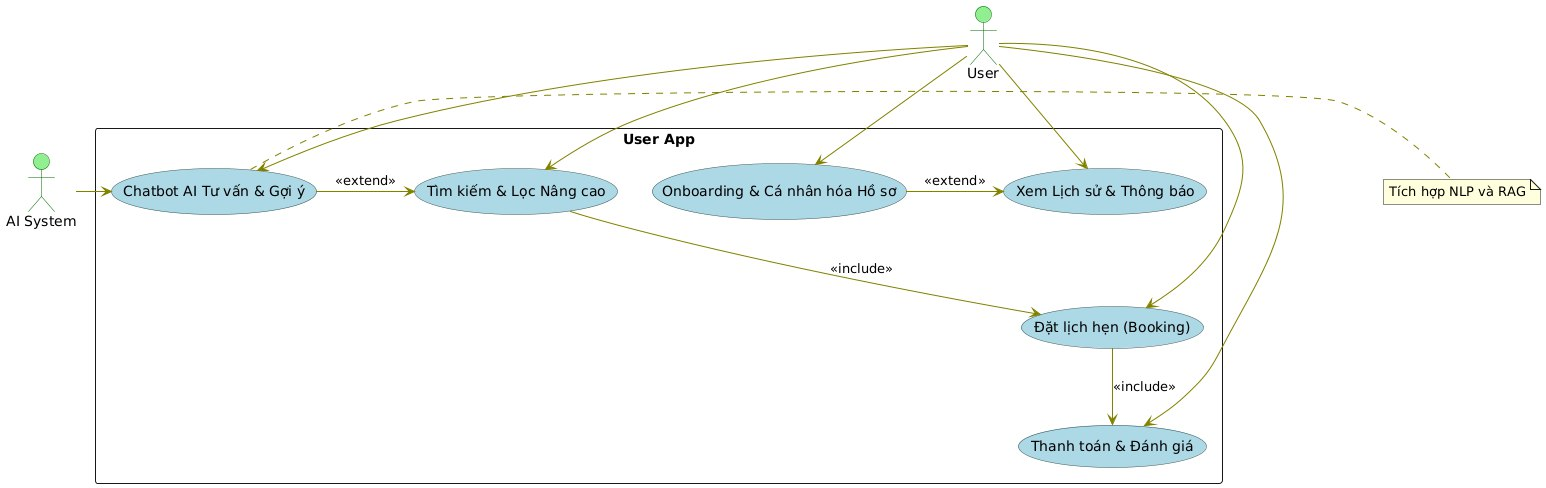
\includegraphics[width=0.8\textwidth]{Images/User_Usecase.jpg}
    \vspace{10pt}
    
    % Thêm chú thích cho hình ảnh
    \caption{Sơ đồ Use Case cho User App}
    
    % Đặt nhãn để tham chiếu chéo (cross-reference)
    \label{fig:usecase_user_app}
\end{figure}

\subsection{Sơ đồ Use Case cho Partner Portal}
Sơ đồ này tập trung vào các chức năng quản lý dành cho nhà cung cấp dịch vụ (Service Providers), bao gồm đăng ký, quản lý lịch hẹn, dịch vụ, nhân viên và báo cáo (theo Phần 3.1.2).

\begin{figure}[H]
    % Căn giữa hình ảnh
    \centering
    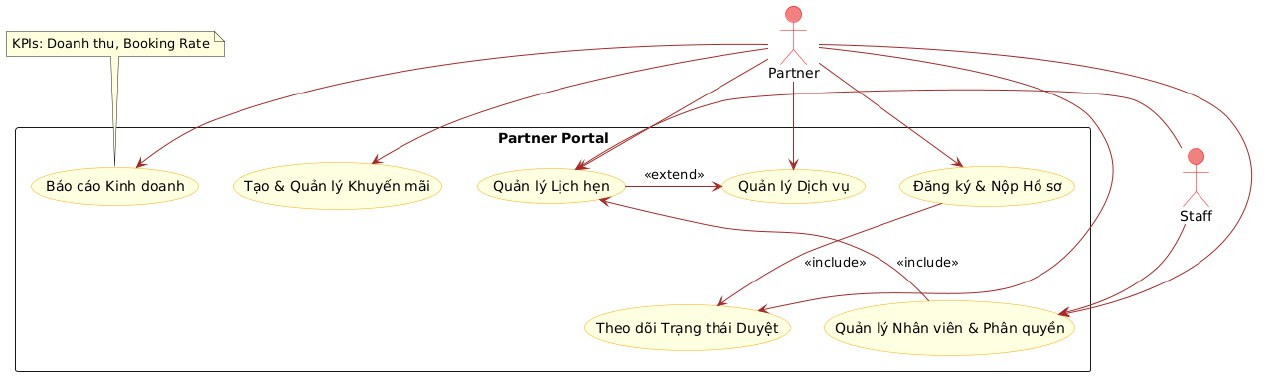
\includegraphics[width=0.8\textwidth]{Images/Partner_Usecase.jpg}
    \vspace{10pt}
    
    % Thêm chú thích cho hình ảnh
    \caption{Sơ đồ Use Case cho Partner Portal}
    
    % Đặt nhãn để tham chiếu chéo (cross-reference)
    \label{fig:usecase_partner_portal}
\end{figure}

\subsection{Sơ đồ Use Case cho Admin Dashboard}
Sơ đồ này mô tả các chức năng quản trị hệ thống, bao gồm xác thực đối tác, quản lý đánh giá, tài chính, voucher và hỗ trợ (theo Phần 3.1.3).

\begin{figure}[H]
    % Căn giữa hình ảnh
    \centering
    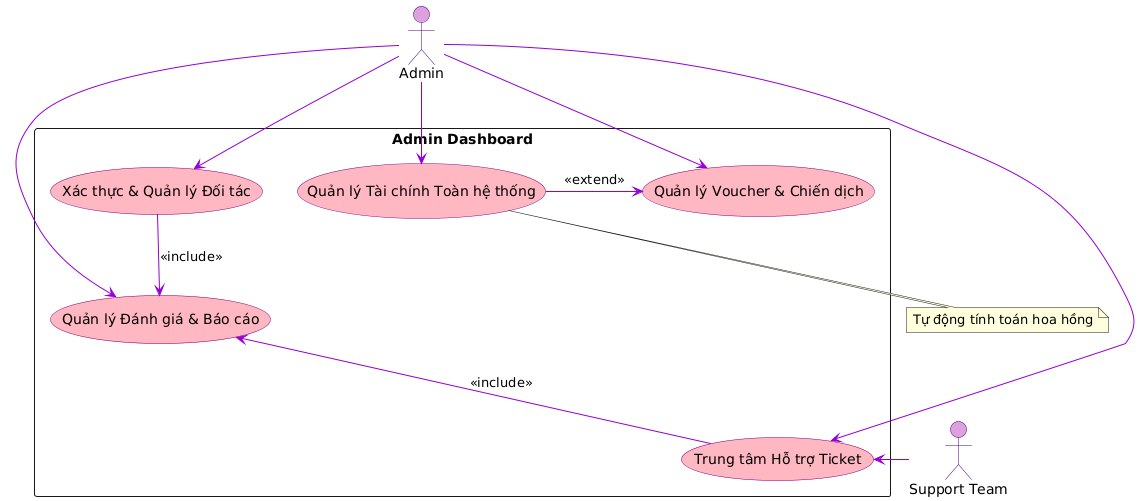
\includegraphics[width=0.8\textwidth]{Images/Admin_Usecase.jpg}
    \vspace{10pt}
    
    % Thêm chú thích cho hình ảnh
    \caption{Sơ đồ Use Case cho Admin Dashboard}
    
    % Đặt nhãn để tham chiếu chéo (cross-reference)
    \label{fig:usecase_admin_dashboard}
\end{figure}

\subsection{Sơ đồ Use Case Tổng Thể Hệ Thống (Tích Hợp AI)}
Sơ đồ này thể hiện tổng quan hệ thống, nhấn mạnh vai trò của AI trong cá nhân hóa và hỗ trợ (dựa trên Phần 5 Phần AI).
\begin{figure}[H]
    % Căn giữa hình ảnh
    \centering
    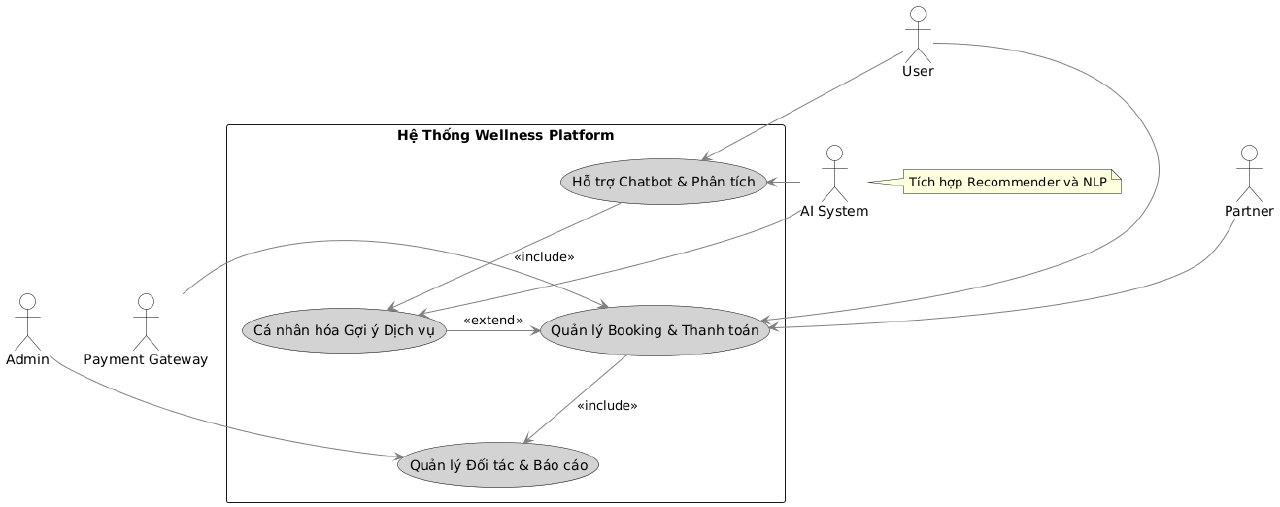
\includegraphics[width=0.8\textwidth]{Images/Wellness_Usecase.jpg}
    \vspace{10pt}
    
    % Thêm chú thích cho hình ảnh
    \caption{Sơ đồ Use Case Tổng Thể Hệ Thống (Tích Hợp AI)}
    
    % Đặt nhãn để tham chiếu chéo (cross-reference)
    \label{fig:usecase_overall}
\end{figure}

\section{Chi Tiết Use Case (Use-case Detail)}

\subsection{Use Case 1: Onboarding và Cá nhân hóa Hồ sơ (User App)}

\begin{table}[H]
\centering
\begin{tabular}{|p{3cm}|p{12cm}|}
\hline
\textbf{Tên use case:} & Onboarding và Cá nhân hóa Hồ sơ \\
\hline
\textbf{Vai trò:} & Người dùng (End User) \\
\hline
\textbf{Mô tả:} & Hệ thống cho phép người dùng đăng ký tài khoản và hoàn thành khảo sát ban đầu để tạo hồ sơ cá nhân hóa, từ đó đề xuất dịch vụ phù hợp ngay từ đầu (dựa trên Phần 3.1.1). \\
\hline
\textbf{Tiền điều kiện:} & 
\begin{itemize}
\item Ứng dụng di động (User App) được mở và người dùng chưa có tài khoản.
\item Kết nối internet ổn định.
\end{itemize} \\
\hline
\textbf{Hậu điều kiện:} & 
\begin{itemize}
\item Hồ sơ người dùng được tạo và lưu trữ an toàn trong cơ sở dữ liệu (Phần 4.3 ERD).
\item Gợi ý dịch vụ cá nhân hóa được hiển thị dựa trên dữ liệu khảo sát.
\end{itemize} \\
\hline
\textbf{Luồng sự kiện chính:} & 
\begin{itemize}
\item Người dùng chọn phương thức đăng ký (username/password, Google/Facebook).
\item Hệ thống xác thực và gửi email/SMS xác nhận.
\item Người dùng hoàn thành khảo sát ngắn gọn về nhu cầu (ví dụ: loại da, vấn đề sức khỏe như căng thẳng, đau vai gáy).
\item Hệ thống xử lý dữ liệu khảo sát qua AI (Recommender System, Phần 5.3) để tạo hồ sơ và đề xuất dịch vụ đầu tiên (spa thư giãn, y học cổ truyền).
\item Chuyển hướng đến trang chính với gợi ý cá nhân hóa.
\end{itemize} \\
\hline
\textbf{Luồng thay thế:} & 
\begin{enumerate}
\item[a.] Nếu người dùng chọn đăng ký qua mạng xã hội, hệ thống tự động điền thông tin cơ bản và bỏ qua bước nhập thủ công.
\item[b.] Nếu khảo sát bị bỏ qua, hệ thống sử dụng dữ liệu mặc định và nhắc nhở hoàn thành sau.
\item[c.] Nếu dữ liệu khảo sát thay đổi, hệ thống cập nhật hồ sơ thời gian thực và điều chỉnh gợi ý.
\end{enumerate} \\
\hline
\textbf{Ngoại lệ:} & 
\begin{itemize}
\item Nếu xác thực thất bại (email không hợp lệ), hiển thị lỗi và yêu cầu thử lại.
\item Nếu mất kết nối, lưu tiến trình tạm thời và khôi phục khi kết nối lại.
\item Nếu dữ liệu cá nhân nhạy cảm (lịch sử sức khỏe) bị từ chối, hệ thống xóa và không lưu trữ.
\end{itemize} \\
\hline
\end{tabular}
\caption{Use Case 1: Onboarding và Cá nhân hóa Hồ sơ.}
\label{tab:uc1}
\end{table}

\subsection{Use Case 2: Chatbot AI Tư vấn và Gợi ý Dịch vụ (User App)}

\begin{table}[H]
\centering
\begin{tabular}{|p{3cm}|p{12cm}|}
\hline
\textbf{Tên use case:} & Chatbot AI Tư vấn và Gợi ý Dịch vụ \\
\hline
\textbf{Vai trò:} & Người dùng (End User) và Hệ thống AI \\
\hline
\textbf{Mô tả:} & Người dùng trò chuyện với chatbot AI để nhận tư vấn dựa trên NLP, phân tích triệu chứng và gợi ý dịch vụ phù hợp (spa, y học cổ truyền, vật lý trị liệu theo Phần 3.1.1 và Phần 5.2). \\
\hline
\textbf{Tiền điều kiện:} & 
\begin{itemize}
\item Người dùng đã đăng nhập và mở giao diện chatbot.
\item Hệ thống AI (NLP và RAG) đã được khởi tạo (Phần 5.2.4).
\end{itemize} \\
\hline
\textbf{Hậu điều kiện:} & 
\begin{itemize}
\item Gợi ý dịch vụ được lưu vào lịch sử hội thoại và cập nhật hồ sơ người dùng.
\item Người dùng được điều hướng đến trang đặt lịch nếu chấp nhận gợi ý.
\end{itemize} \\
\hline
\textbf{Luồng sự kiện chính:} & 
\begin{itemize}
\item Người dùng khởi tạo phiên chat bằng câu hỏi (ví dụ: "Tôi bị đau vai gáy").
\item Hệ thống AI sử dụng NLP để phân loại ý định và truy xuất dữ liệu (RAG từ cơ sở kiến thức, Phần 5.2.5).
\item AI đặt câu hỏi làm rõ (ví dụ: vị trí, mức độ nghiêm trọng) và gợi ý dịch vụ (bấm huyệt, massage trị liệu với chi tiết giá, đánh giá, vị trí).
\item Người dùng xác nhận gợi ý, hệ thống gửi thông báo và liên kết đến trang booking.
\end{itemize} \\
\hline
\textbf{Luồng thay thế:} & 
\begin{enumerate}
\item[a.] Nếu hội thoại đa lượt, AI duy trì ngữ cảnh (multi-turn, Phần 5.2.3) để tinh chỉnh gợi ý.
\item[b.] Nếu không có gợi ý phù hợp, AI đề xuất tìm kiếm nâng cao hoặc kết nối hỗ trợ con người.
\item[c.] Nếu người dùng cung cấp vị trí, tích hợp bản đồ để ưu tiên đối tác gần nhất.
\end{enumerate} \\
\hline
\textbf{Ngoại lệ:} & 
\begin{itemize}
\item Nếu truy vấn không rõ ràng hoặc hallucination (Phần 5.2.6), AI yêu cầu làm rõ hoặc chuyển sang tìm kiếm thủ công.
\item Nếu lỗi kết nối AI, fallback sang FAQ tĩnh.
\item Nếu nội dung nhạy cảm (y tế chuyên sâu), cảnh báo và khuyên tư vấn bác sĩ.
\end{itemize} \\
\hline
\end{tabular}
\caption{Use Case 2: Chatbot AI Tư vấn và Gợi ý Dịch vụ.}
\label{tab:uc2}
\end{table}

\subsection{Use Case 3: Đặt lịch hẹn (Booking) (User App)}

\begin{table}[H]
\centering
\begin{tabular}{|p{3cm}|p{12cm}|}
\hline
\textbf{Tên use case:} & Đặt lịch hẹn (Booking) \\
\hline
\textbf{Vai trò:} & Người dùng (End User) và Đối tác (Service Provider) \\
\hline
\textbf{Mô tả:} & Người dùng chọn dịch vụ, xem lịch trống thời gian thực và đặt lịch, với thông báo tự động cho cả hai bên (Phần 3.1.1 và Phần 4.2.4). \\
\hline
\textbf{Tiền điều kiện:} & 
\begin{itemize}
\item Người dùng đã chọn dịch vụ từ tìm kiếm hoặc gợi ý AI.
\item Đối tác đã được xác thực và có lịch trống (Phần 3.1.3).
\end{itemize} \\
\hline
\textbf{Hậu điều kiện:} & 
\begin{itemize}
\item Lịch hẹn được xác nhận và cập nhật trong cơ sở dữ liệu (ERD, Phần 4.3).
\item Thông báo đẩy/email được gửi, và lịch sử booking được cập nhật cho người dùng.
\end{itemize} \\
\hline
\textbf{Luồng sự kiện chính:} & 
\begin{itemize}
\item Người dùng chọn dịch vụ và xem lịch trống thời gian thực từ đối tác.
\item Chọn khung giờ khả dụng và xác nhận (bao gồm thông tin cá nhân nếu cần).
\item Hệ thống kiểm tra tính khả dụng, đặt chỗ tạm thời và gửi yêu cầu xác nhận đến đối tác.
\item Đối tác xác nhận, hệ thống hoàn tất và gửi thông báo cho người dùng.
\end{itemize} \\
\hline
\textbf{Luồng thay thế:} & 
\begin{enumerate}
\item[a.] Nếu thanh toán trước, tích hợp payment gateway (MoMo, Phần 1.3.2) trước khi xác nhận.
\item[b.] Nếu hủy trong 24 giờ, tự động giải phóng slot và hoàn tiền.
\item[c.] Nếu thay đổi lịch, gửi yêu cầu cập nhật đến đối tác.
\end{enumerate} \\
\hline
\textbf{Ngoại lệ:} & 
\begin{itemize}
\item Nếu slot hết, hiển thị thông báo và gợi ý slot thay thế.
\item Nếu đối tác từ chối, hoàn tiền và thông báo lý do.
\item Nếu lỗi hệ thống (load cao, Phần 3.2), retry sau 30 giây.
\end{itemize} \\
\hline
\end{tabular}
\caption{Use Case 3: Đặt lịch hẹn (Booking).}
\label{tab:uc3}
\end{table}

\subsection{Use Case 4: Trang Đăng ký Cung cấp Hồ sơ (Partner Portal)}

\begin{table}[H]
\centering
\begin{tabular}{|p{3cm}|p{12cm}|}
\hline
\textbf{Tên use case:} & Trang Đăng ký Cung cấp Hồ sơ (Partner Registration) \\
\hline
\textbf{Vai trò:} & Đối tác (Service Provider) \\
\hline
\textbf{Mô tả:} & Đối tác cung cấp thông tin kinh doanh và tài liệu pháp lý để đăng ký tham gia nền tảng (Phần 3.1.2 và Phần 4.2.7). \\
\hline
\textbf{Tiền điều kiện:} & 
\begin{itemize}
\item Đối tác truy cập Partner Portal qua web/app.
\item Hệ thống xác thực cơ bản (email).
\end{itemize} \\
\hline
\textbf{Hậu điều kiện:} & 
\begin{itemize}
\item Hồ sơ được lưu và chuyển sang trạng thái "Chờ duyệt".
\item Email xác nhận được gửi với hướng dẫn theo dõi.
\end{itemize} \\
\hline
\textbf{Luồng sự kiện chính:} & 
\begin{itemize}
\item Đối tác điền biểu mẫu đa bước (thông tin doanh nghiệp, mô tả dịch vụ).
\item Tải lên tài liệu (giấy phép kinh doanh, chứng chỉ hành nghề).
\item Hệ thống kiểm tra định dạng và gửi xác nhận.
\item Chuyển đến Limited Partner Portal để theo dõi duyệt.
\end{itemize} \\
\hline
\textbf{Luồng thay thế:} & 
\begin{enumerate}
\item[a.] Nếu tải tài liệu thất bại, cho phép thử lại mà không mất dữ liệu.
\item[b.] Nếu hồ sơ đầy đủ, tự động ưu tiên duyệt nhanh.
\item[c.] Nếu bổ sung sau, cập nhật và thông báo admin.
\end{enumerate} \\
\hline
\textbf{Ngoại lệ:} & 
\begin{itemize}
\item Nếu tài liệu không hợp lệ (định dạng sai), hiển thị lỗi cụ thể.
\item Nếu trùng lặp thông tin, cảnh báo và yêu cầu chỉnh sửa.
\item Nếu vi phạm chính sách (dịch vụ xâm lấn, Phần 1.3.1), từ chối ngay.
\end{itemize} \\
\hline
\end{tabular}
\caption{Use Case 4: Trang Đăng ký Cung cấp Hồ sơ.}
\label{tab:uc4}
\end{table}

\subsection{Use Case 5: Xác thực Quản lý Đối tác (Admin Dashboard)}

\begin{table}[H]
\centering
\begin{tabular}{|p{3cm}|p{12cm}|}
\hline
\textbf{Tên use case:} & Xác thực Quản lý Đối tác (Partner Verification Management) \\
\hline
\textbf{Vai trò:} & Quản trị viên (Admin) \\
\hline
\textbf{Mô tả:} & Admin xem xét và phê duyệt hồ sơ đối tác để đảm bảo chất lượng (Phần 3.1.3 và Phần 4.2.14). \\
\hline
\textbf{Tiền điều kiện:} & 
\begin{itemize}
\item Hồ sơ đối tác ở trạng thái "Chờ duyệt" trong Admin Dashboard.
\item Admin đã đăng nhập với quyền cao.
\end{itemize} \\
\hline
\textbf{Hậu điều kiện:} & 
\begin{itemize}
\item Hồ sơ được phê duyệt/từ chối và cập nhật trạng thái.
\item Đối tác nhận thông báo và quyền truy cập tương ứng.
\end{itemize} \\
\hline
\textbf{Luồng sự kiện chính:} & 
\begin{itemize}
\item Admin xem danh sách hồ sơ mới với tài liệu đính kèm.
\item Kiểm tra thông tin pháp lý và chất lượng dịch vụ.
\item Chọn hành động: Phê duyệt (mở khóa đầy đủ), Từ chối (với lý do), hoặc Yêu cầu bổ sung.
\item Hệ thống cập nhật và gửi thông báo/email.
\end{itemize} \\
\hline
\textbf{Luồng thay thế:} & 
\begin{enumerate}
\item[a.] Nếu yêu cầu bổ sung, đối tác nhận thông báo qua Limited Portal.
\item[b.] Nếu phê duyệt hàng loạt, xử lý nhiều hồ sơ cùng lúc.
\item[c.] Nếu từ chối, lưu lý do để báo cáo thống kê.
\end{enumerate} \\
\hline
\textbf{Ngoại lệ:} & 
\begin{itemize}
\item Nếu tài liệu giả mạo, khóa tạm thời và báo cáo pháp lý.
\item Nếu lỗi tải tài liệu, yêu cầu đối tác tải lại.
\item Nếu vượt quá thời hạn duyệt (7 ngày), tự động từ chối.
\end{itemize} \\
\hline
\end{tabular}
\caption{Use Case 5: Xác thực Quản lý Đối tác.}
\label{tab:uc5}
\end{table}

\section{Sơ đồ luồng dữ liệu (Sequence Diagram)}
Các sơ đồ tuần tự (Sequence Diagrams) dưới đây mô tả chi tiết luồng tương tác giữa các thành phần trong hệ thống Healthcare Platform, bao gồm tương tác giữa người dùng, ứng dụng di động, API Gateway, các microservices backend, cơ sở dữ liệu và các dịch vụ bên ngoài.

\subsection{Onboarding 
\& Cá nhân hóa Hồ sơ}
\begin{figure}[H]
    % Căn giữa hình ảnh
    \centering
    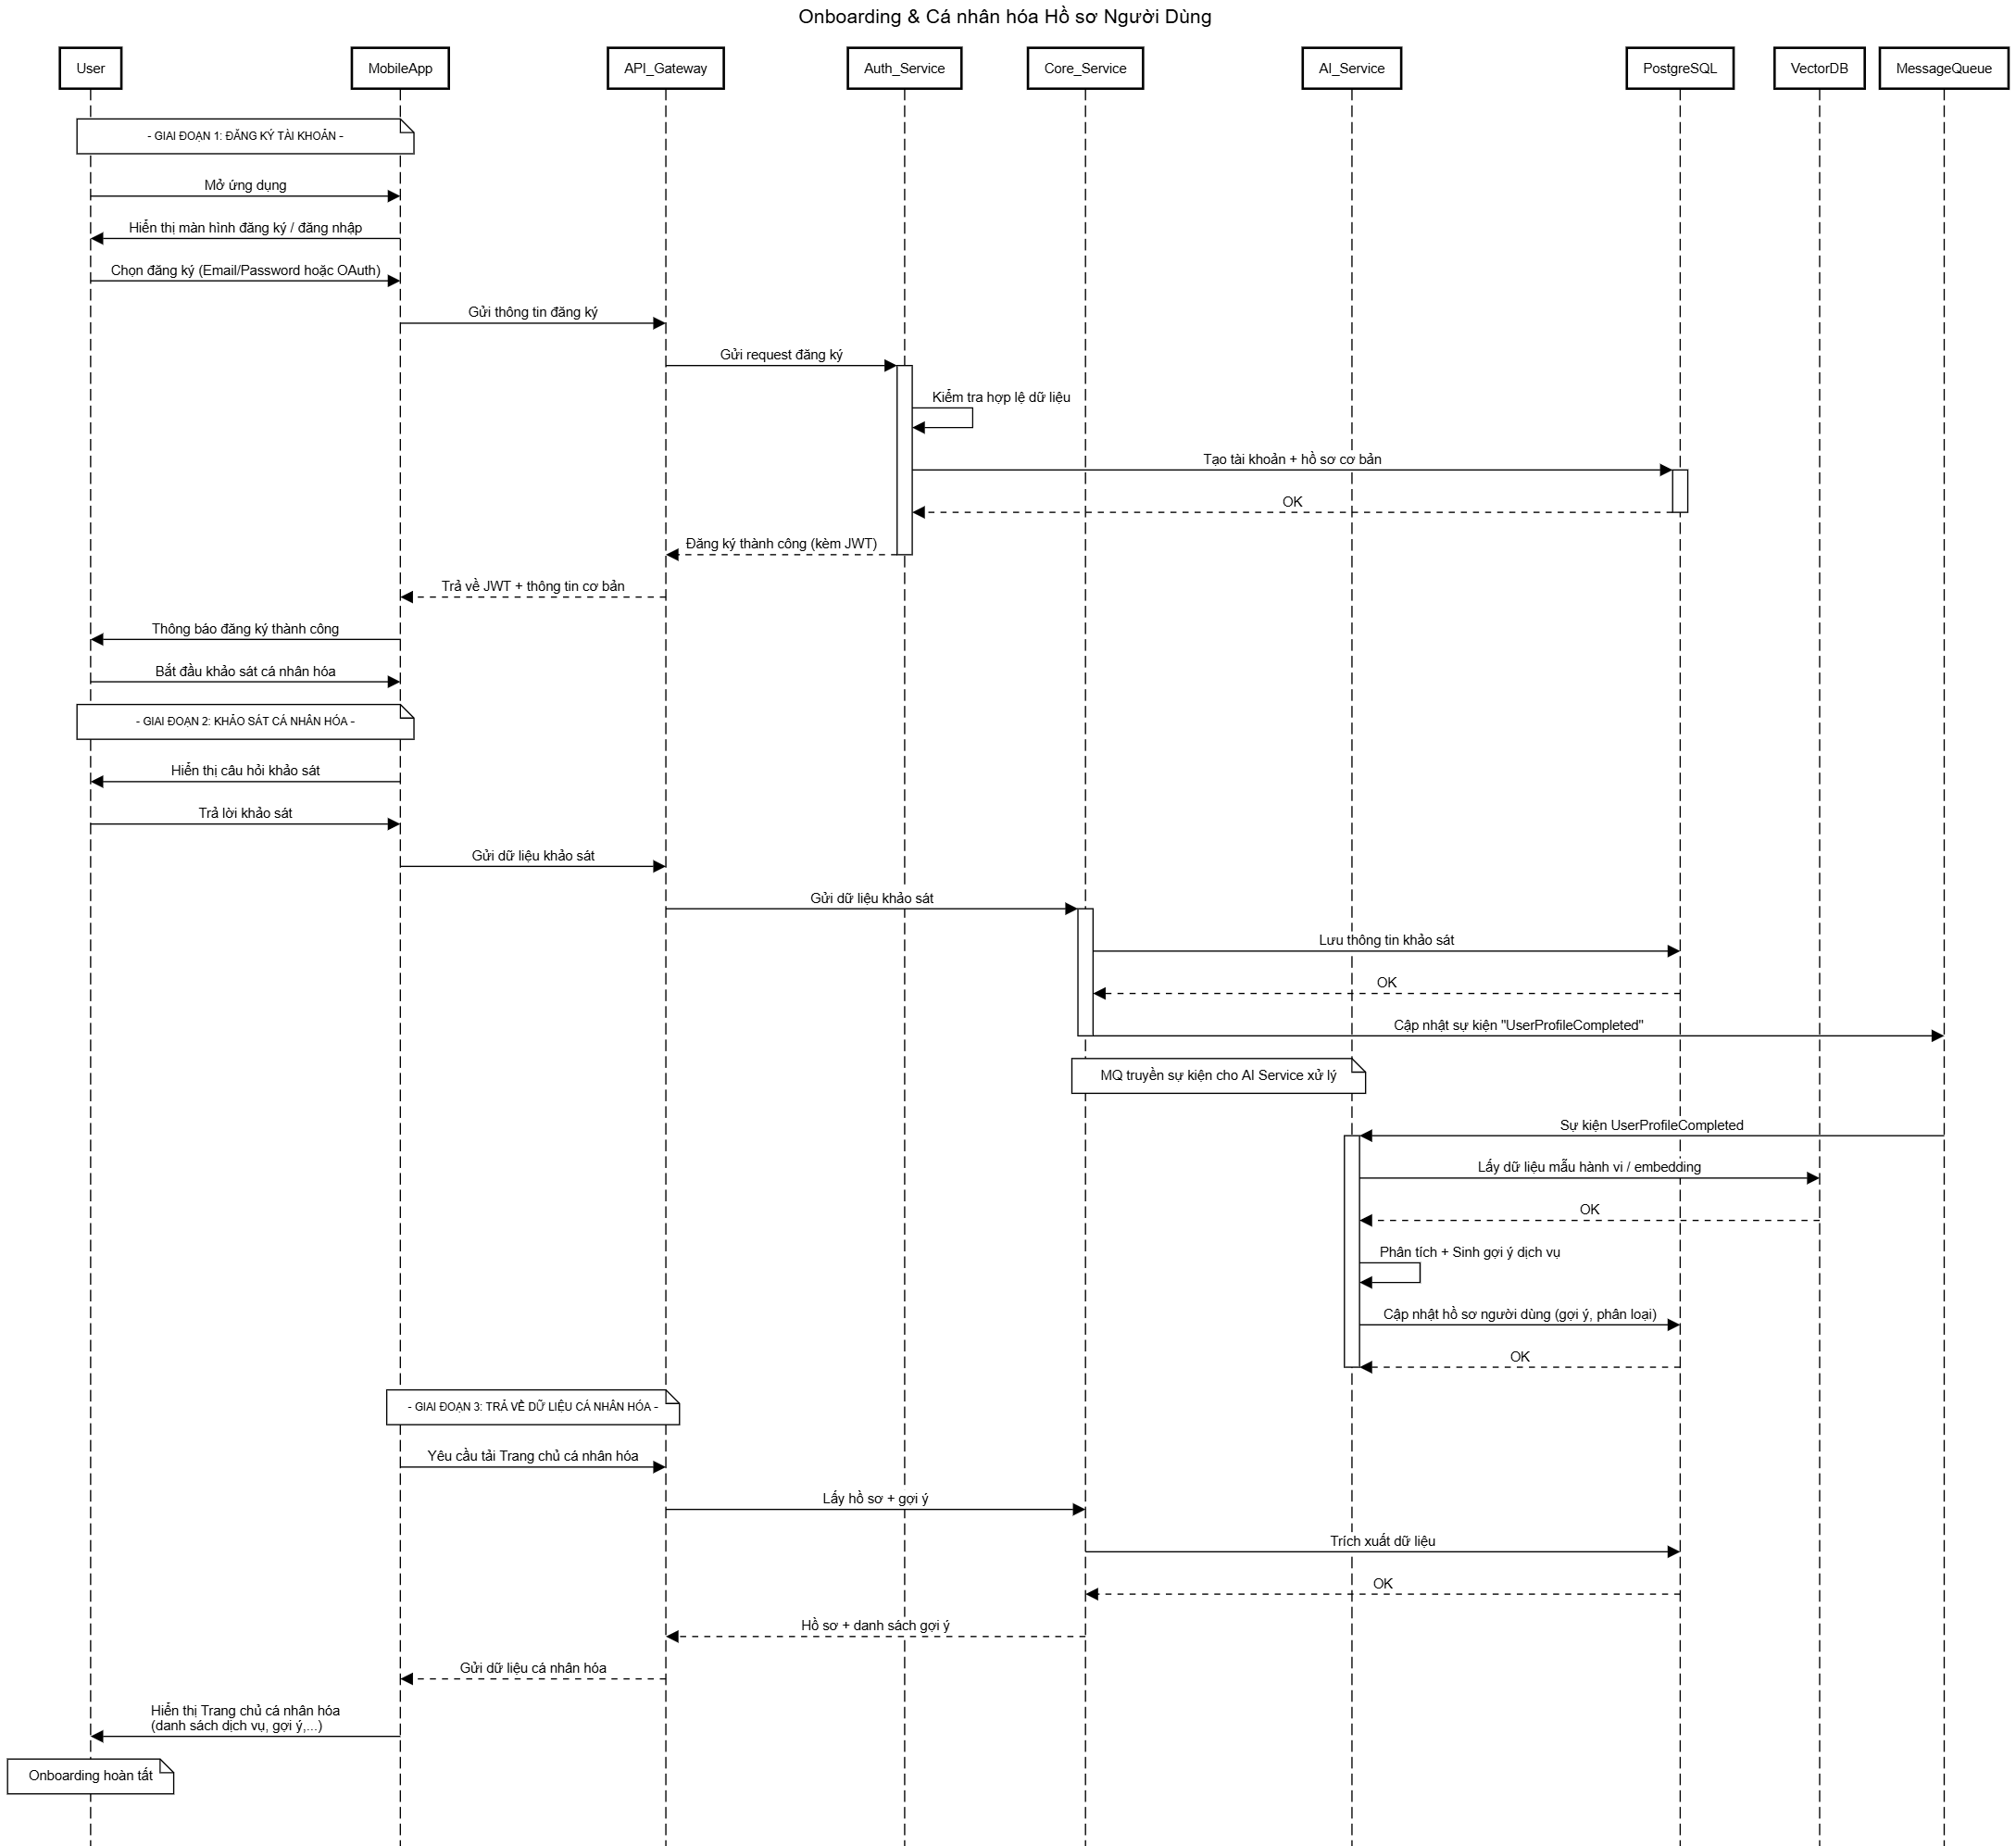
\includegraphics[width=0.8\textwidth]{Images/sequences/4.2.1.png}
    \vspace{10pt}
    
    % Thêm chú thích cho hình ảnh
    \caption{Đăng ký và cá nhân hoá}
    
    % Đặt nhãn để tham chiếu chéo (cross-reference)
    \label{fig:onboarding_personalize}
\end{figure}
Hình \ref{fig:onboarding_personalize} mô tả quy trình đăng ký và cá nhân hóa hồ sơ người dùng. Quy trình bắt đầu khi người dùng mở ứng dụng và lựa chọn phương thức đăng ký (Email/Password hoặc OAuth). Sau khi xác thực thành công qua Auth\_Service, hệ thống yêu cầu người dùng hoàn thành khảo sát cá nhân hóa. AI\_Service xử lý thông tin khảo sát để tạo hồ sơ người dùng (UserProfileCompleted), phân tích sở thích và đề xuất dịch vụ phù hợp. Dữ liệu được lưu trữ trong VectorDB và MessageQueue để phục vụ cho các tính năng gợi ý sau này. Cuối cùng, người dùng được chuyển đến trang chủ với các dịch vụ được cá nhân hóa.

\subsection{Chatbot AI Tư vấn \& Gợi ý Dịch vụ}
\begin{figure}[H]
    % Căn giữa hình ảnh
    \centering
    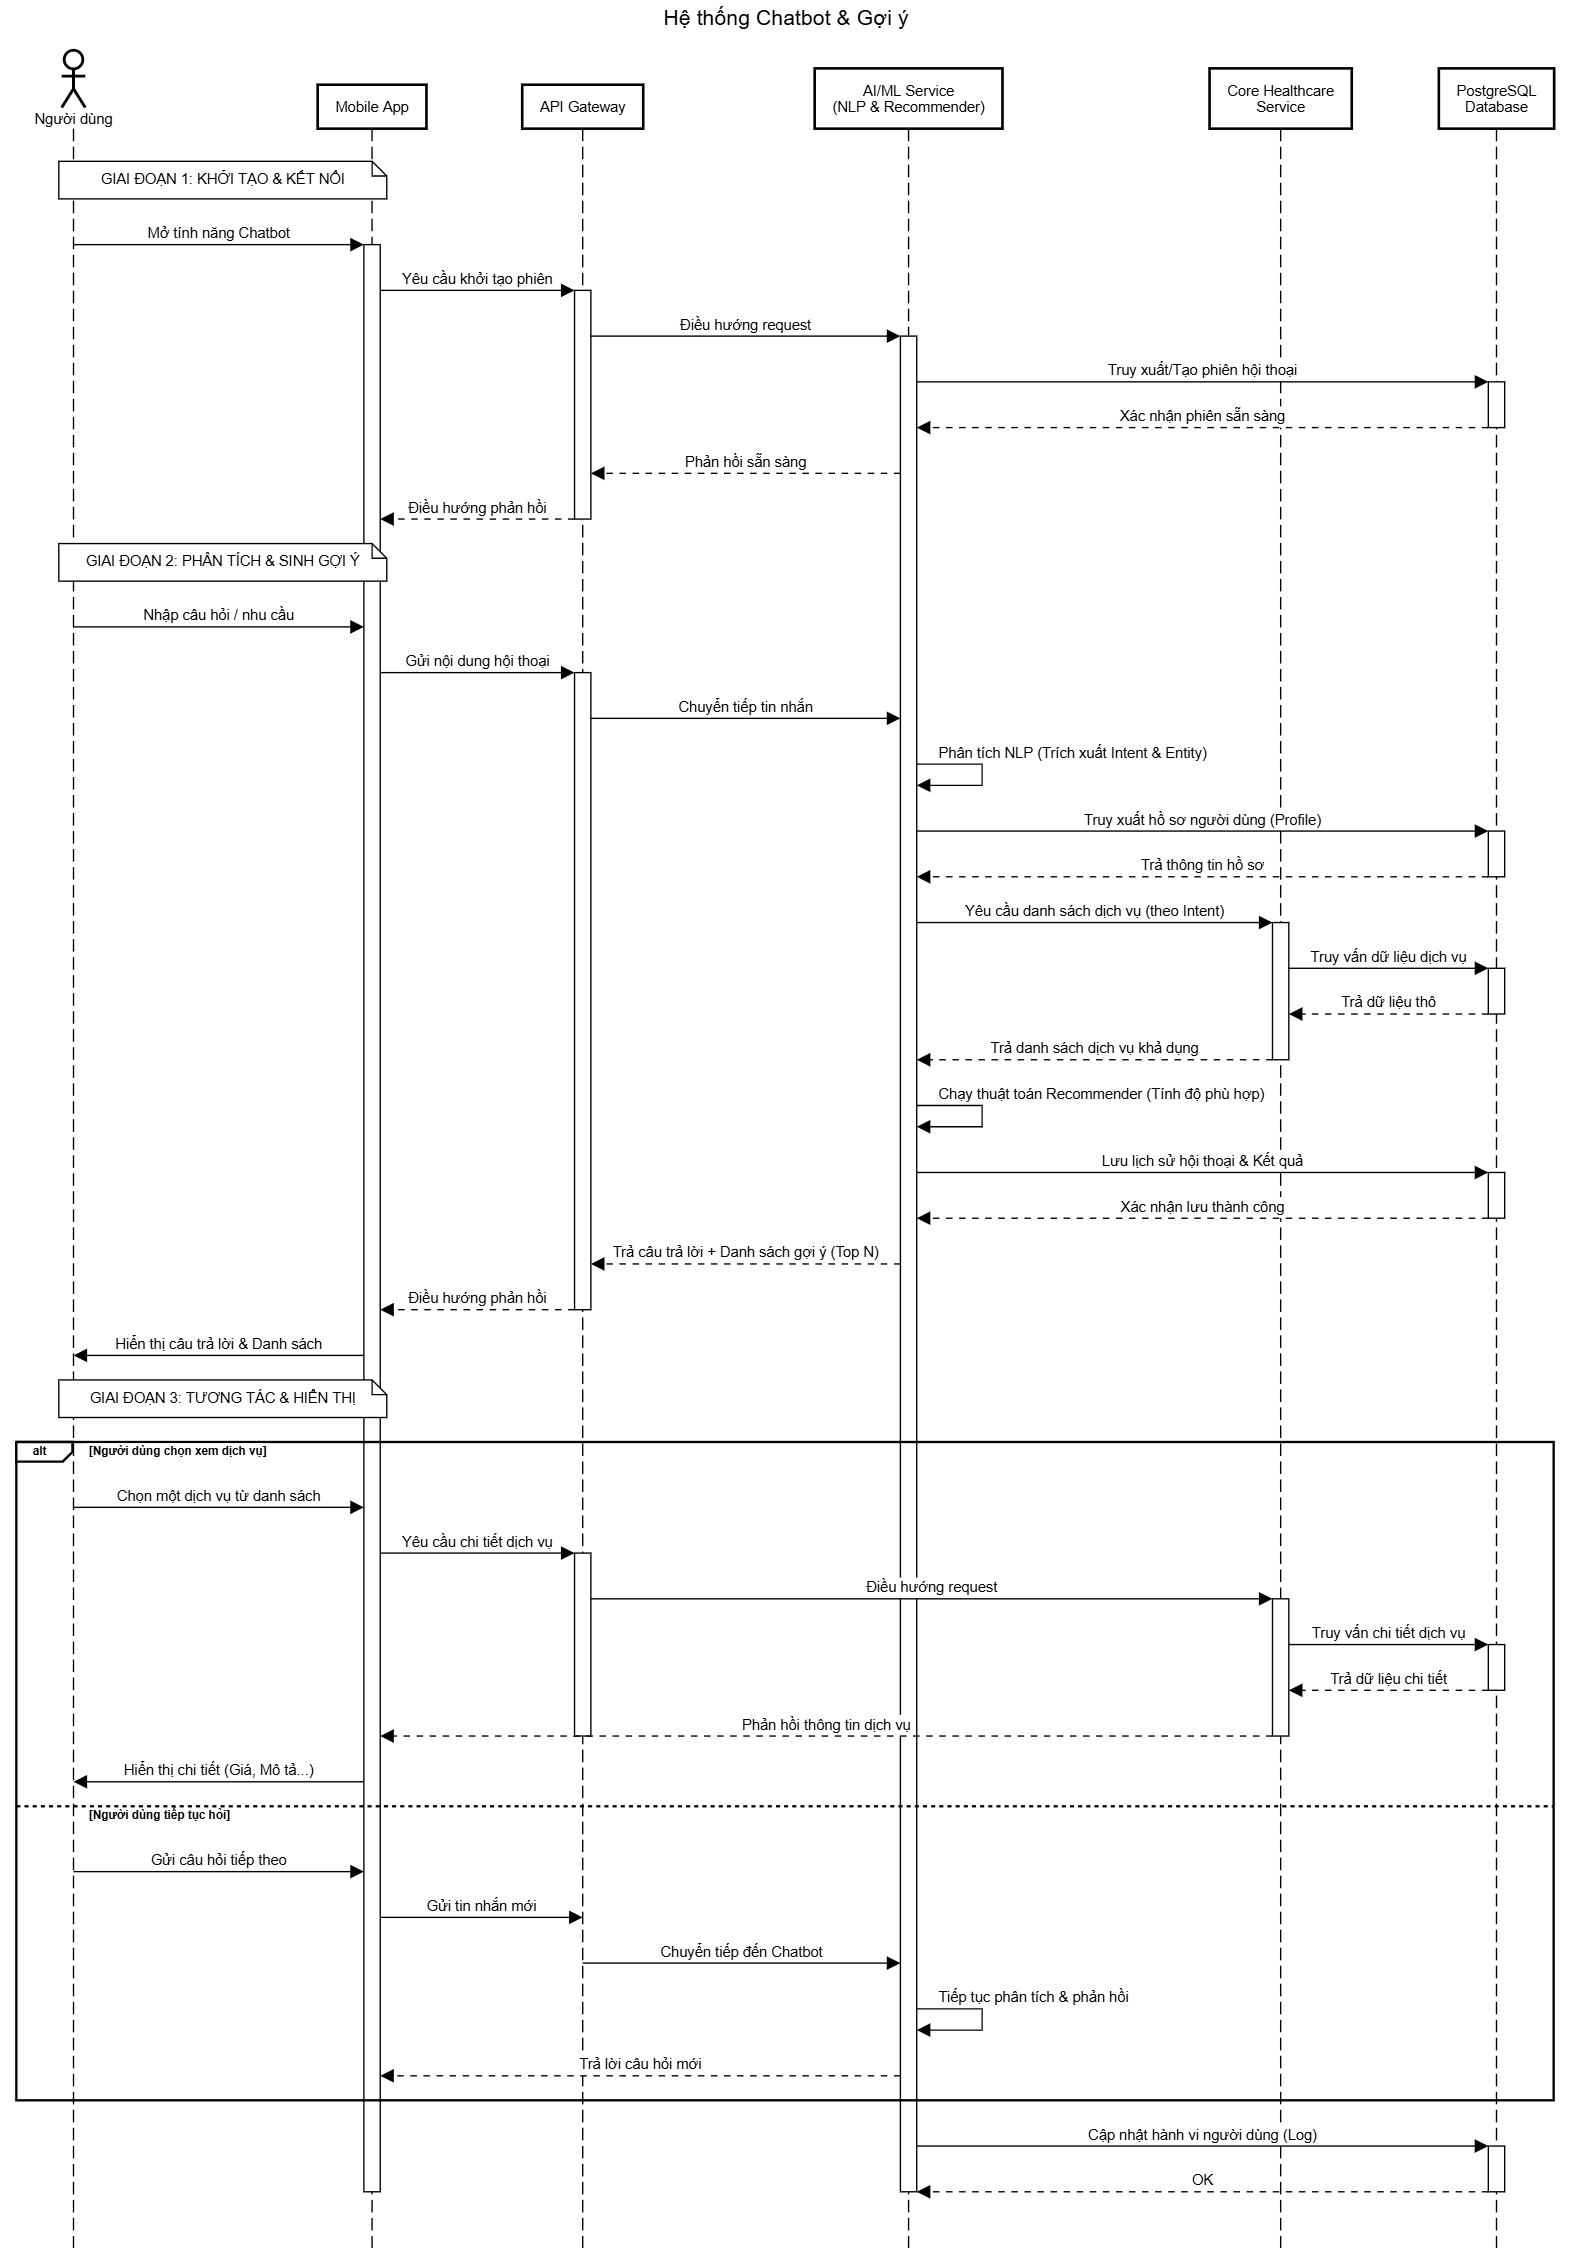
\includegraphics[width=0.8\textwidth]{Images/sequences/4.2.2.png}
    \vspace{10pt}
    
    % Thêm chú thích cho hình ảnh
    \caption{Chatbot AI \& Tư vấn}
    
    % Đặt nhãn để tham chiếu chéo (cross-reference)
    \label{fig:seq_chatbot_ai}
\end{figure}
Hình \ref{fig:seq_chatbot_ai} thể hiện luồng tương tác với chatbot AI hỗ trợ tư vấn sức khỏe. Quy trình được chia thành 3 giai đoạn chính: (1) Khởi tạo và kết nối chatbot thông qua API Gateway đến AI\_Service (NLP \& Recommender); (2) Phân tích và sinh gợi ý - hệ thống sử dụng NLP để phân tích intent và entity từ câu hỏi người dùng, truy xuất thông tin từ Core Healthcare Service, sau đó chạy thuật toán Recommender để đưa ra danh sách dịch vụ phù hợp (Top-N); (3) Tương tác và hiển thị - người dùng có thể chọn xem chi tiết từng dịch vụ được gợi ý hoặc gửi tin nhắn mới để chatbot tiếp tục hỗ trợ. Hệ thống ghi nhận toàn bộ lịch sử hội thoại và cập nhật vào cơ sở dữ liệu.


\subsection{Tìm kiếm \& Lọc Nâng cao}
\begin{figure}[H]
    % Căn giữa hình ảnh
    \centering
    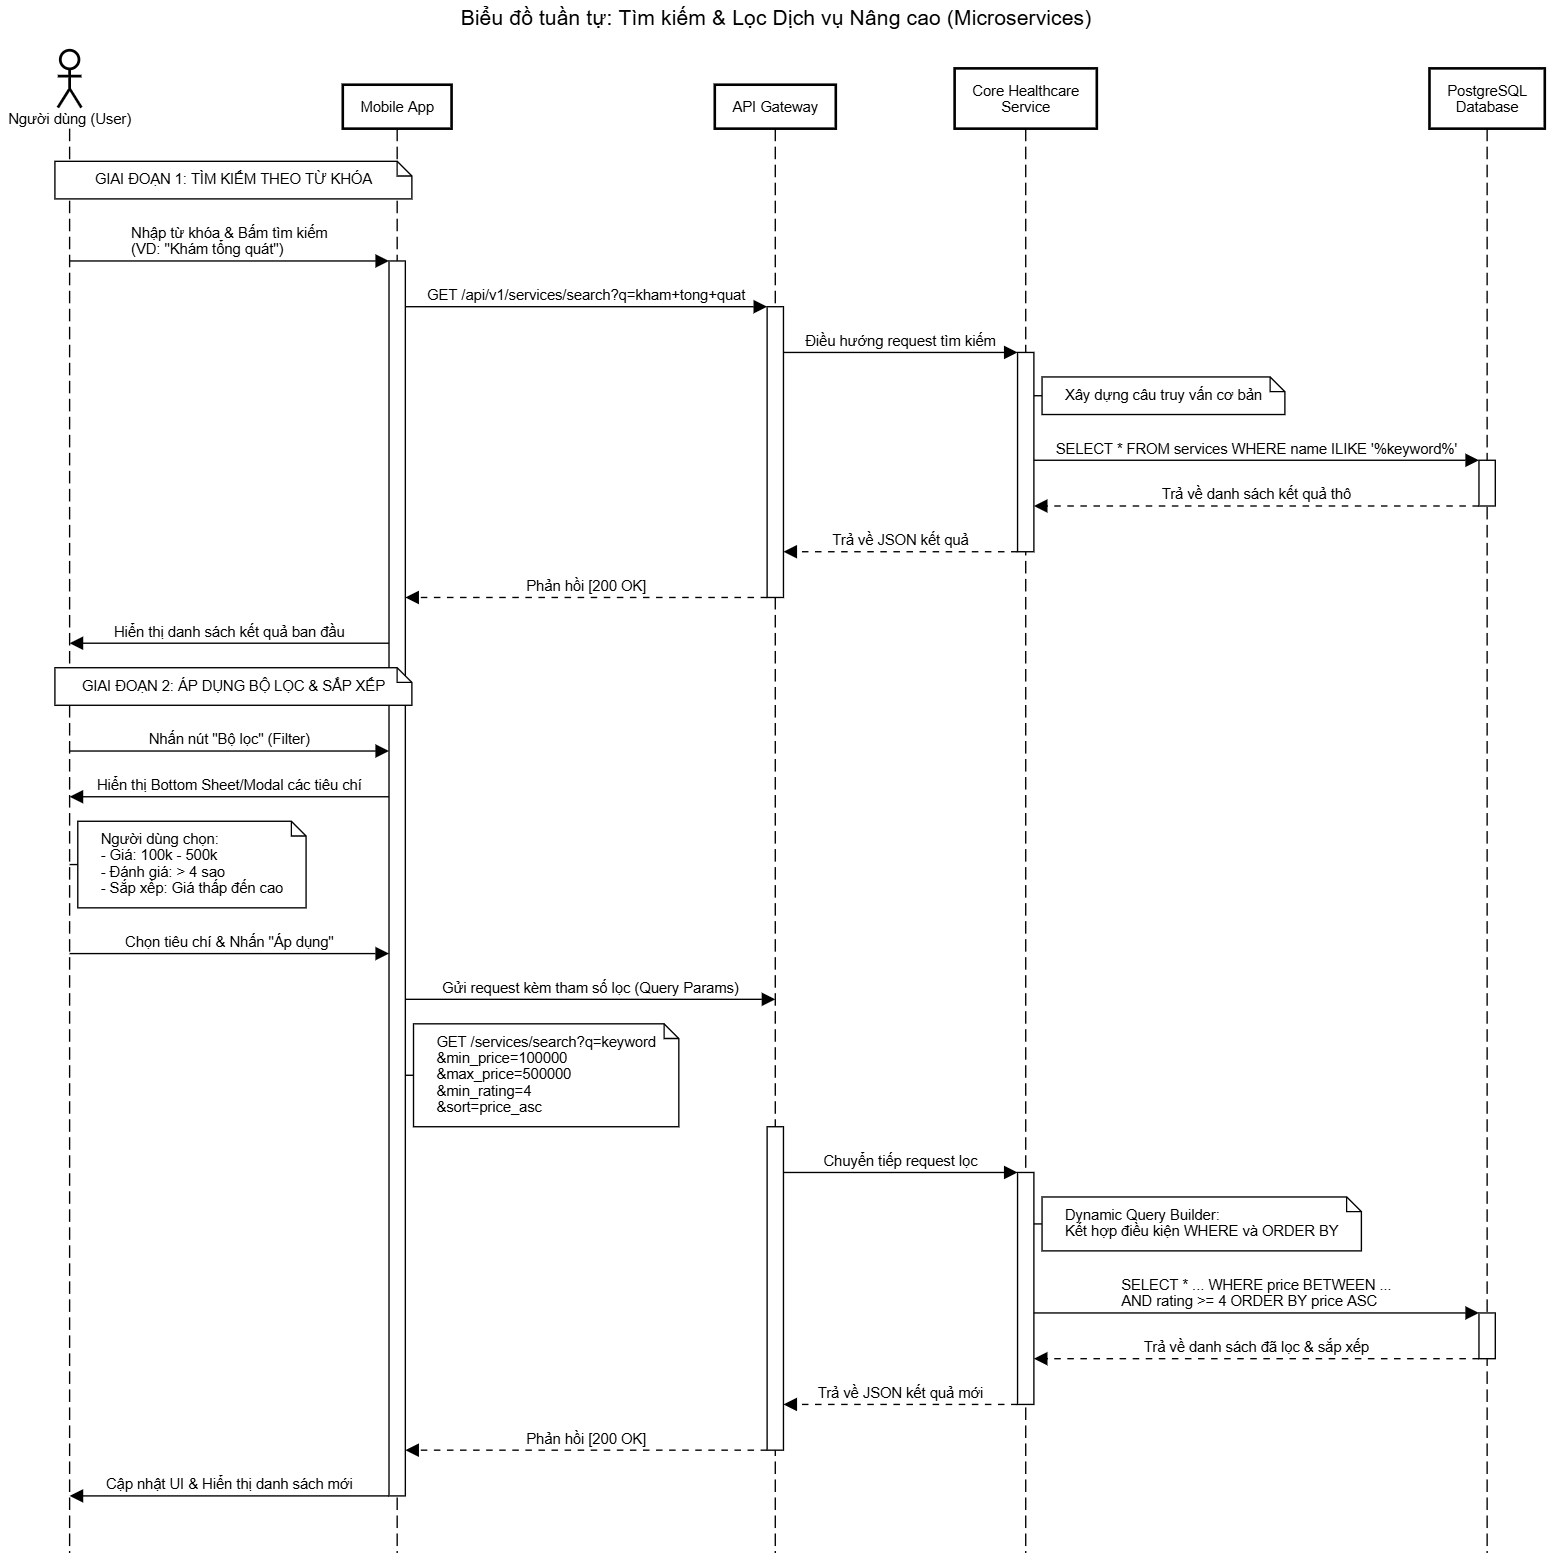
\includegraphics[width=0.8\textwidth]{Images/sequences/4.2.3.png}
    \vspace{10pt}
    
    % Thêm chú thích cho hình ảnh
    \caption{Tìm kiếm \& Lọc Nâng cao}
    
    % Đặt nhãn để tham chiếu chéo (cross-reference)
    \label{fig:seq_search_filter}
\end{figure}
Hình \ref{fig:seq_search_filter} mô tả quy trình tìm kiếm và lọc dịch vụ y tế với các tính năng nâng cao. Giai đoạn 1 thực hiện tìm kiếm theo từ khóa đơn giản, hệ thống xây dựng câu truy vấn cơ bản (SELECT * FROM services WHERE name ILIKE '\%keyword\%') và trả về danh sách kết quả ban đầu. Giai đoạn 2 cho phép người dùng áp dụng các bộ lọc phức tạp (giá, đánh giá, khoảng cách, thời gian), hệ thống sử dụng Dynamic Query Builder để kết hợp các điều kiện WHERE và ORDER BY, sau đó thực hiện truy vấn phức tạp (SELECT * WHERE price BETWEEN ... AND rating >= 4 ORDER BY price ASC) để lọc và sắp xếp kết quả. Cuối cùng, giao diện được cập nhật với danh sách dịch vụ đã lọc.


\subsection{Đặt lịch hẹn (Booking), thanh toán và đánh giá}
\begin{figure}[H]
    % Căn giữa hình ảnh
    \centering
    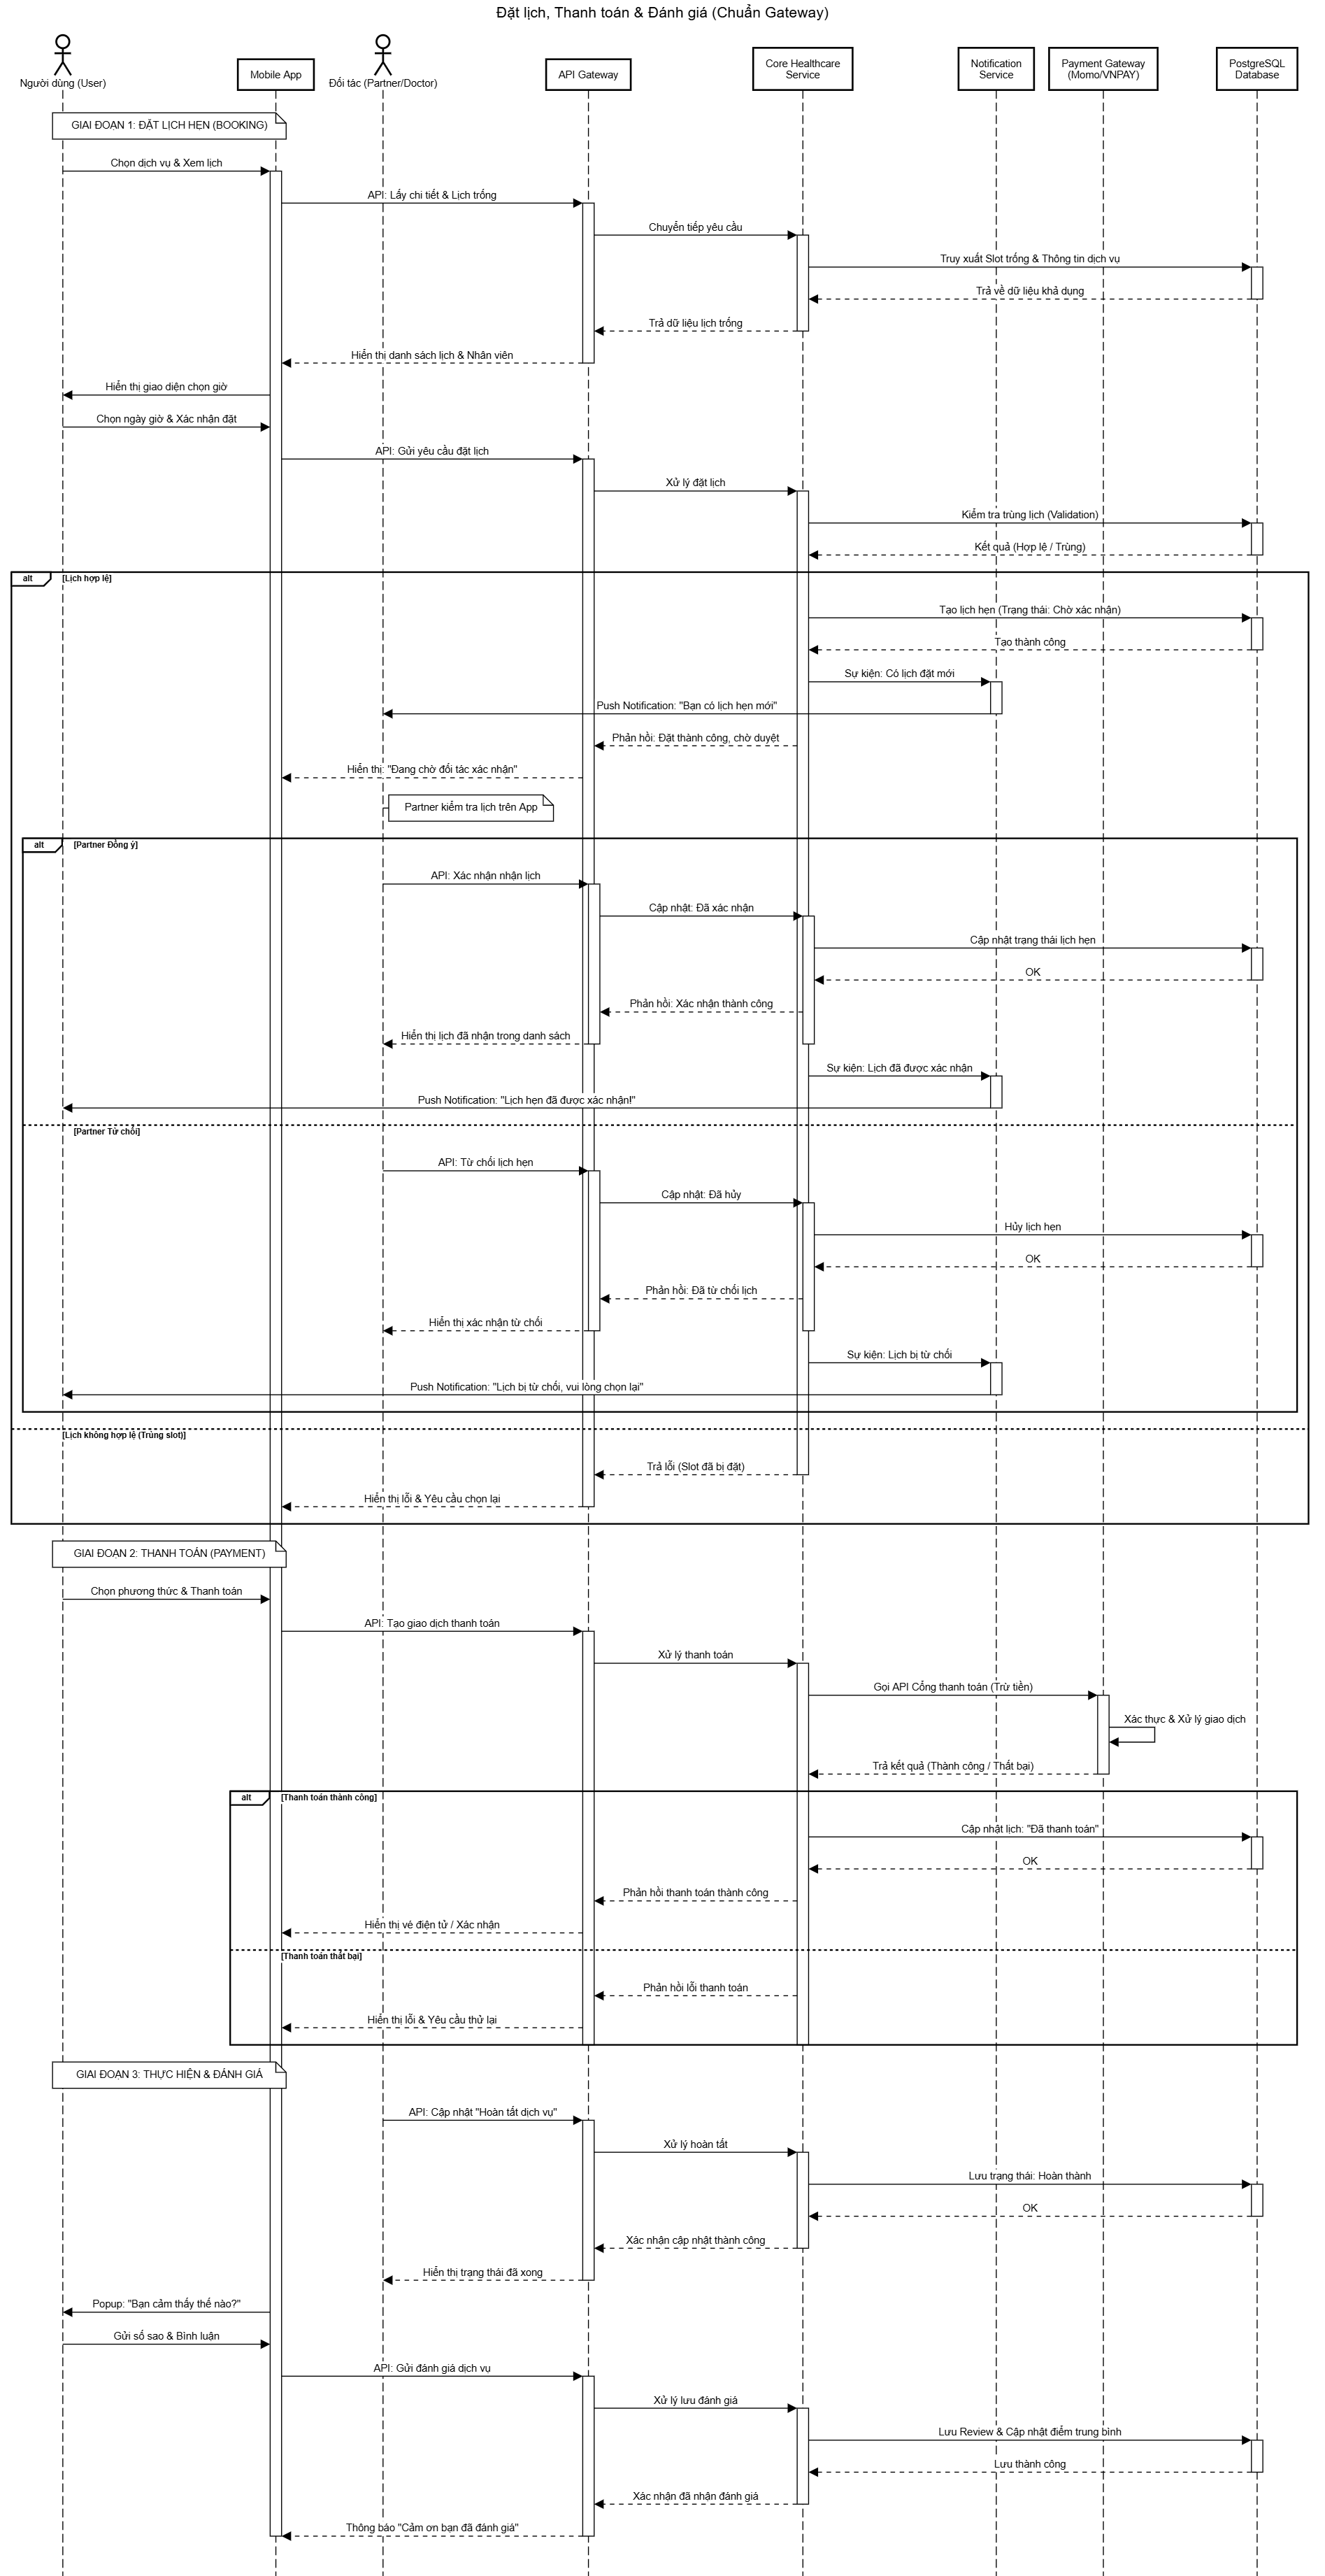
\includegraphics[width=0.7\textwidth]{Images/sequences/4.2.4.png}
    \vspace{10pt}
    
    % Thêm chú thích cho hình ảnh
    \caption{Đặt lịch hẹn (Booking), thanh toán và đánh giá}
    
    % Đặt nhãn để tham chiếu chéo (cross-reference)
    \label{fig:seq_booking_payment}
\end{figure}
Hình \ref{fig:seq_booking_payment} minh họa quy trình đầy đủ từ đặt lịch hẹn đến thanh toán và đánh giá dịch vụ. Quy trình bao gồm 5 giai đoạn: (1) Đặt lịch hẹn (Booking) - người dùng chọn dịch vụ và thời gian, hệ thống truy xuất thông tin slot thời gian khả dụng từ Core Healthcare Service và xác nhận lịch hẹn; (2) Nếu khả dụng, hệ thống khóa slot thời gian tạm thời và gửi push notification cho cả người dùng và đối tác qua Notification Service; (3) Xác nhận lịch hẹn - partner xác nhận và hệ thống ghi nhận vào database, sau đó gửi push notification cập nhật trạng thái; (4) Thanh toán (Payment) - người dùng chọn phương thức thanh toán, Backend API tạo transaction và gọi Payment Gateway (MoMo, VNPay), sau khi thanh toán thành công, hệ thống gửi webhook cập nhật trạng thái thành "PAID" và thông báo đến người dùng; (5) Đánh giá và feedback - sau khi hoàn thành dịch vụ, người dùng có thể gửi đánh giá (rating, comment, hình ảnh), thông tin được lưu vào database và hiển thị thông báo cảm ơn.


\subsection{AI trong Quản trị Tương tác thông minh}
\begin{figure}[H]
    % Căn giữa hình ảnh
    \centering
    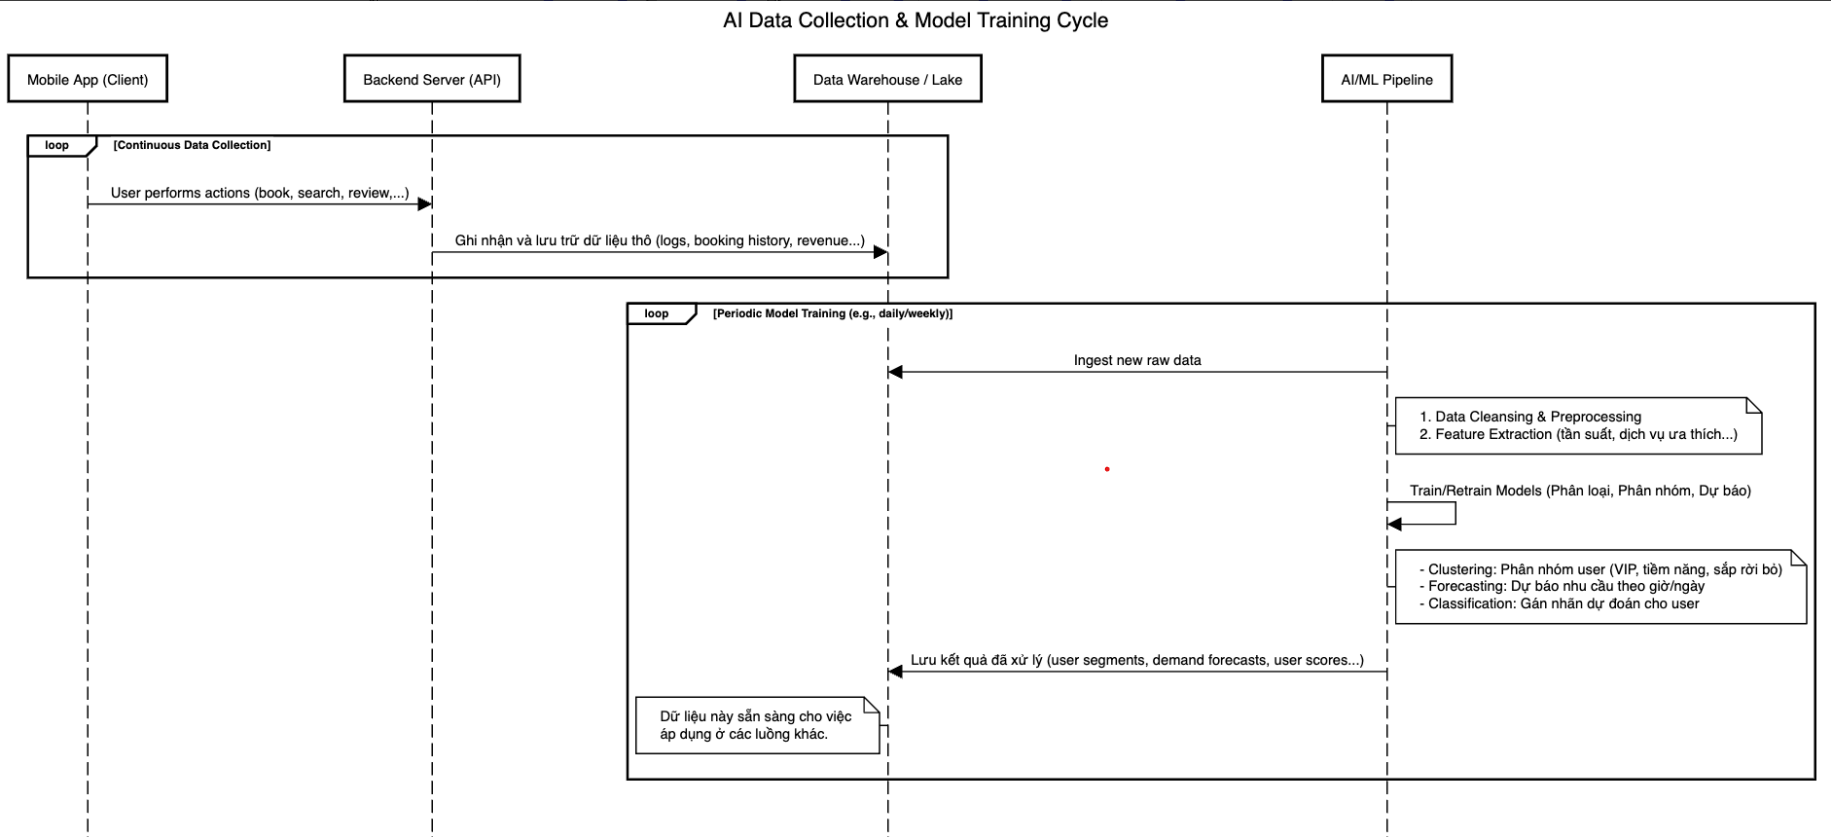
\includegraphics[width=0.8\textwidth]{Images/sequences/4.2.6.png}
    \vspace{10pt}
    
    % Thêm chú thích cho hình ảnh
    \caption{AI trong Quản trị Tương tác thông minh}
    
    % Đặt nhãn để tham chiếu chéo (cross-reference)
    \label{fig:seq_ai_admin}
\end{figure}
Hình \ref{fig:seq_ai_admin} thể hiện cách AI hỗ trợ admin trong việc quản trị hệ thống thông minh qua 3 giai đoạn chính. Giai đoạn 1 - Xem danh sách nhân viên: Admin đăng nhập vào trang quản lý, hệ thống gọi API để lấy danh sách nhân viên từ Core Healthcare Service, truy vấn thông tin chi tiết và hiển thị dưới dạng dashboard. Giai đoạn 2 - Các hành động quản lý (Thêm mới, Sửa, Khóa): Khi admin thực hiện hành động (thêm nhân viên mới, cập nhật thông tin, hoặc khóa tài khoản), hệ thống xử lý request tương ứng, lưu thông tin vào database, cập nhật trạng thái và gửi email thông báo cho nhân viên qua Notification Service. Giai đoạn 3 - Cập nhật hiển thị: Sau mỗi thao tác, dashboard được làm mới để phản ánh thay đổi mới nhất. Toàn bộ quá trình được ghi log để đảm bảo khả năng kiểm tra và truy vết.


\subsection{Trang Đăng ký Cung cấp Hồ sơ (Partner Registration)}
\begin{figure}[H]
    % Căn giữa hình ảnh
    \centering
    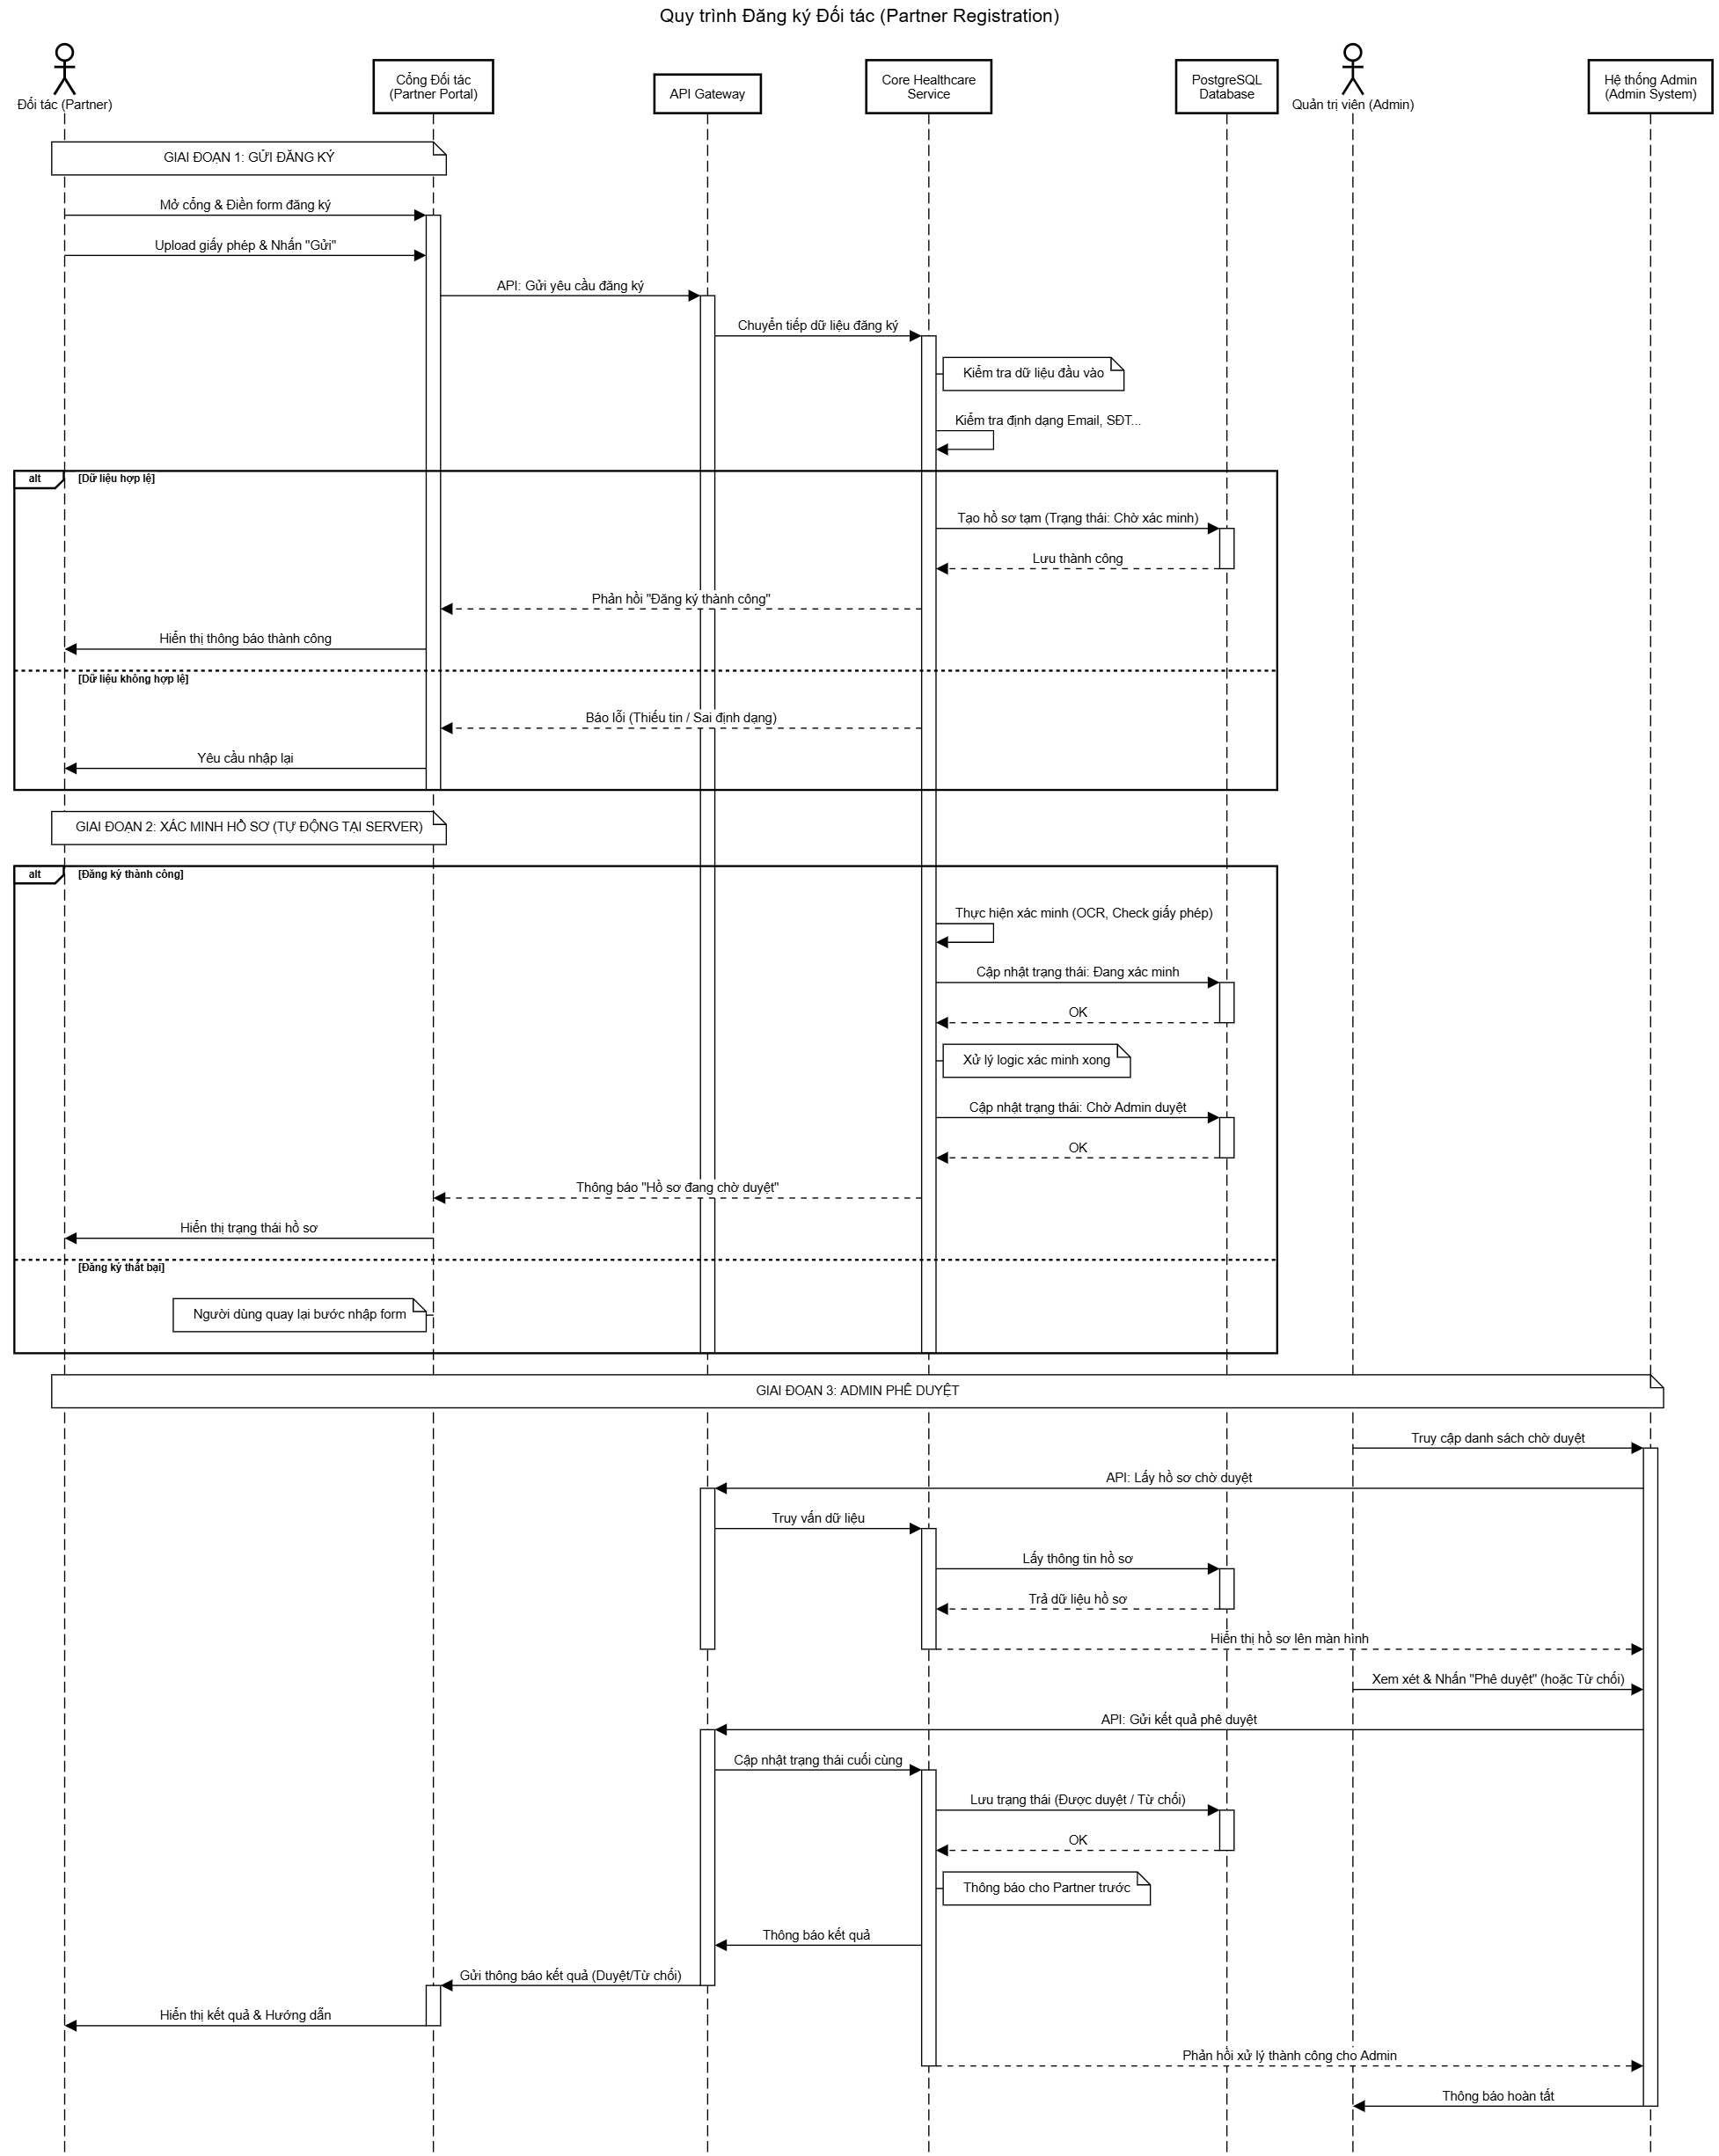
\includegraphics[width=0.8\textwidth]{Images/sequences/4.2.7.png}
    \vspace{10pt}
    
    % Thêm chú thích cho hình ảnh
    \caption{Trang Đăng ký Cung cấp Hồ sơ (Partner Registration)}
    
    % Đặt nhãn để tham chiếu chéo (cross-reference)
    \label{fig:seq_partner_registration}
\end{figure}
Hình \ref{fig:seq_partner_registration} mô tả quy trình đăng ký trở thành đối tác cung cấp dịch vụ y tế trên nền tảng. Quy trình gồm 3 giai đoạn: Giai đoạn 1 - Gửi đăng ký: Đối tác mở cổng đăng ký và điền form thông tin (tên, giấy phép, nhân viên), sau đó upload các giấy tờ chứng minh. API Gateway chuyển request đến Core Healthcare Service để kiểm tra tính hợp lệ và xác thực email SGT (Send Grid Template). Hệ thống tạo hồ sơ mới ở trạng thái "Chờ xác minh" và lưu vào PostgreSQL Database, sau đó phản hồi báo thành công. Giai đoạn 2 - Xác minh hồ sơ từ Server: Hệ thống Admin System nhận request kiểm tra, thực hiện xác minh các trường thông tin (OCR, check giấy phép) và cập nhật trạng thái hồ sơ. Đối tác nhận được thông báo về kết quả xác minh. Giai đoạn 3 - Admin phê duyệt: Admin đăng nhập vào Admin Portal để truy xuất danh sách hồ sơ chờ duyệt, kiểm tra thông tin và đưa ra quyết định phê duyệt. Khi được phê duyệt, hệ thống cập nhật trạng thái "Được duyệt" (Approved), lưu vào database và gửi thông báo kết quả cho đối tác. Đối tác sau đó có thể truy cập Partner Portal để bắt đầu quản lý dịch vụ của mình.

\subsection{Xác thực Đối tác (Partner Verification)}
\begin{figure}[H]
    % Căn giữa hình ảnh
    \centering
    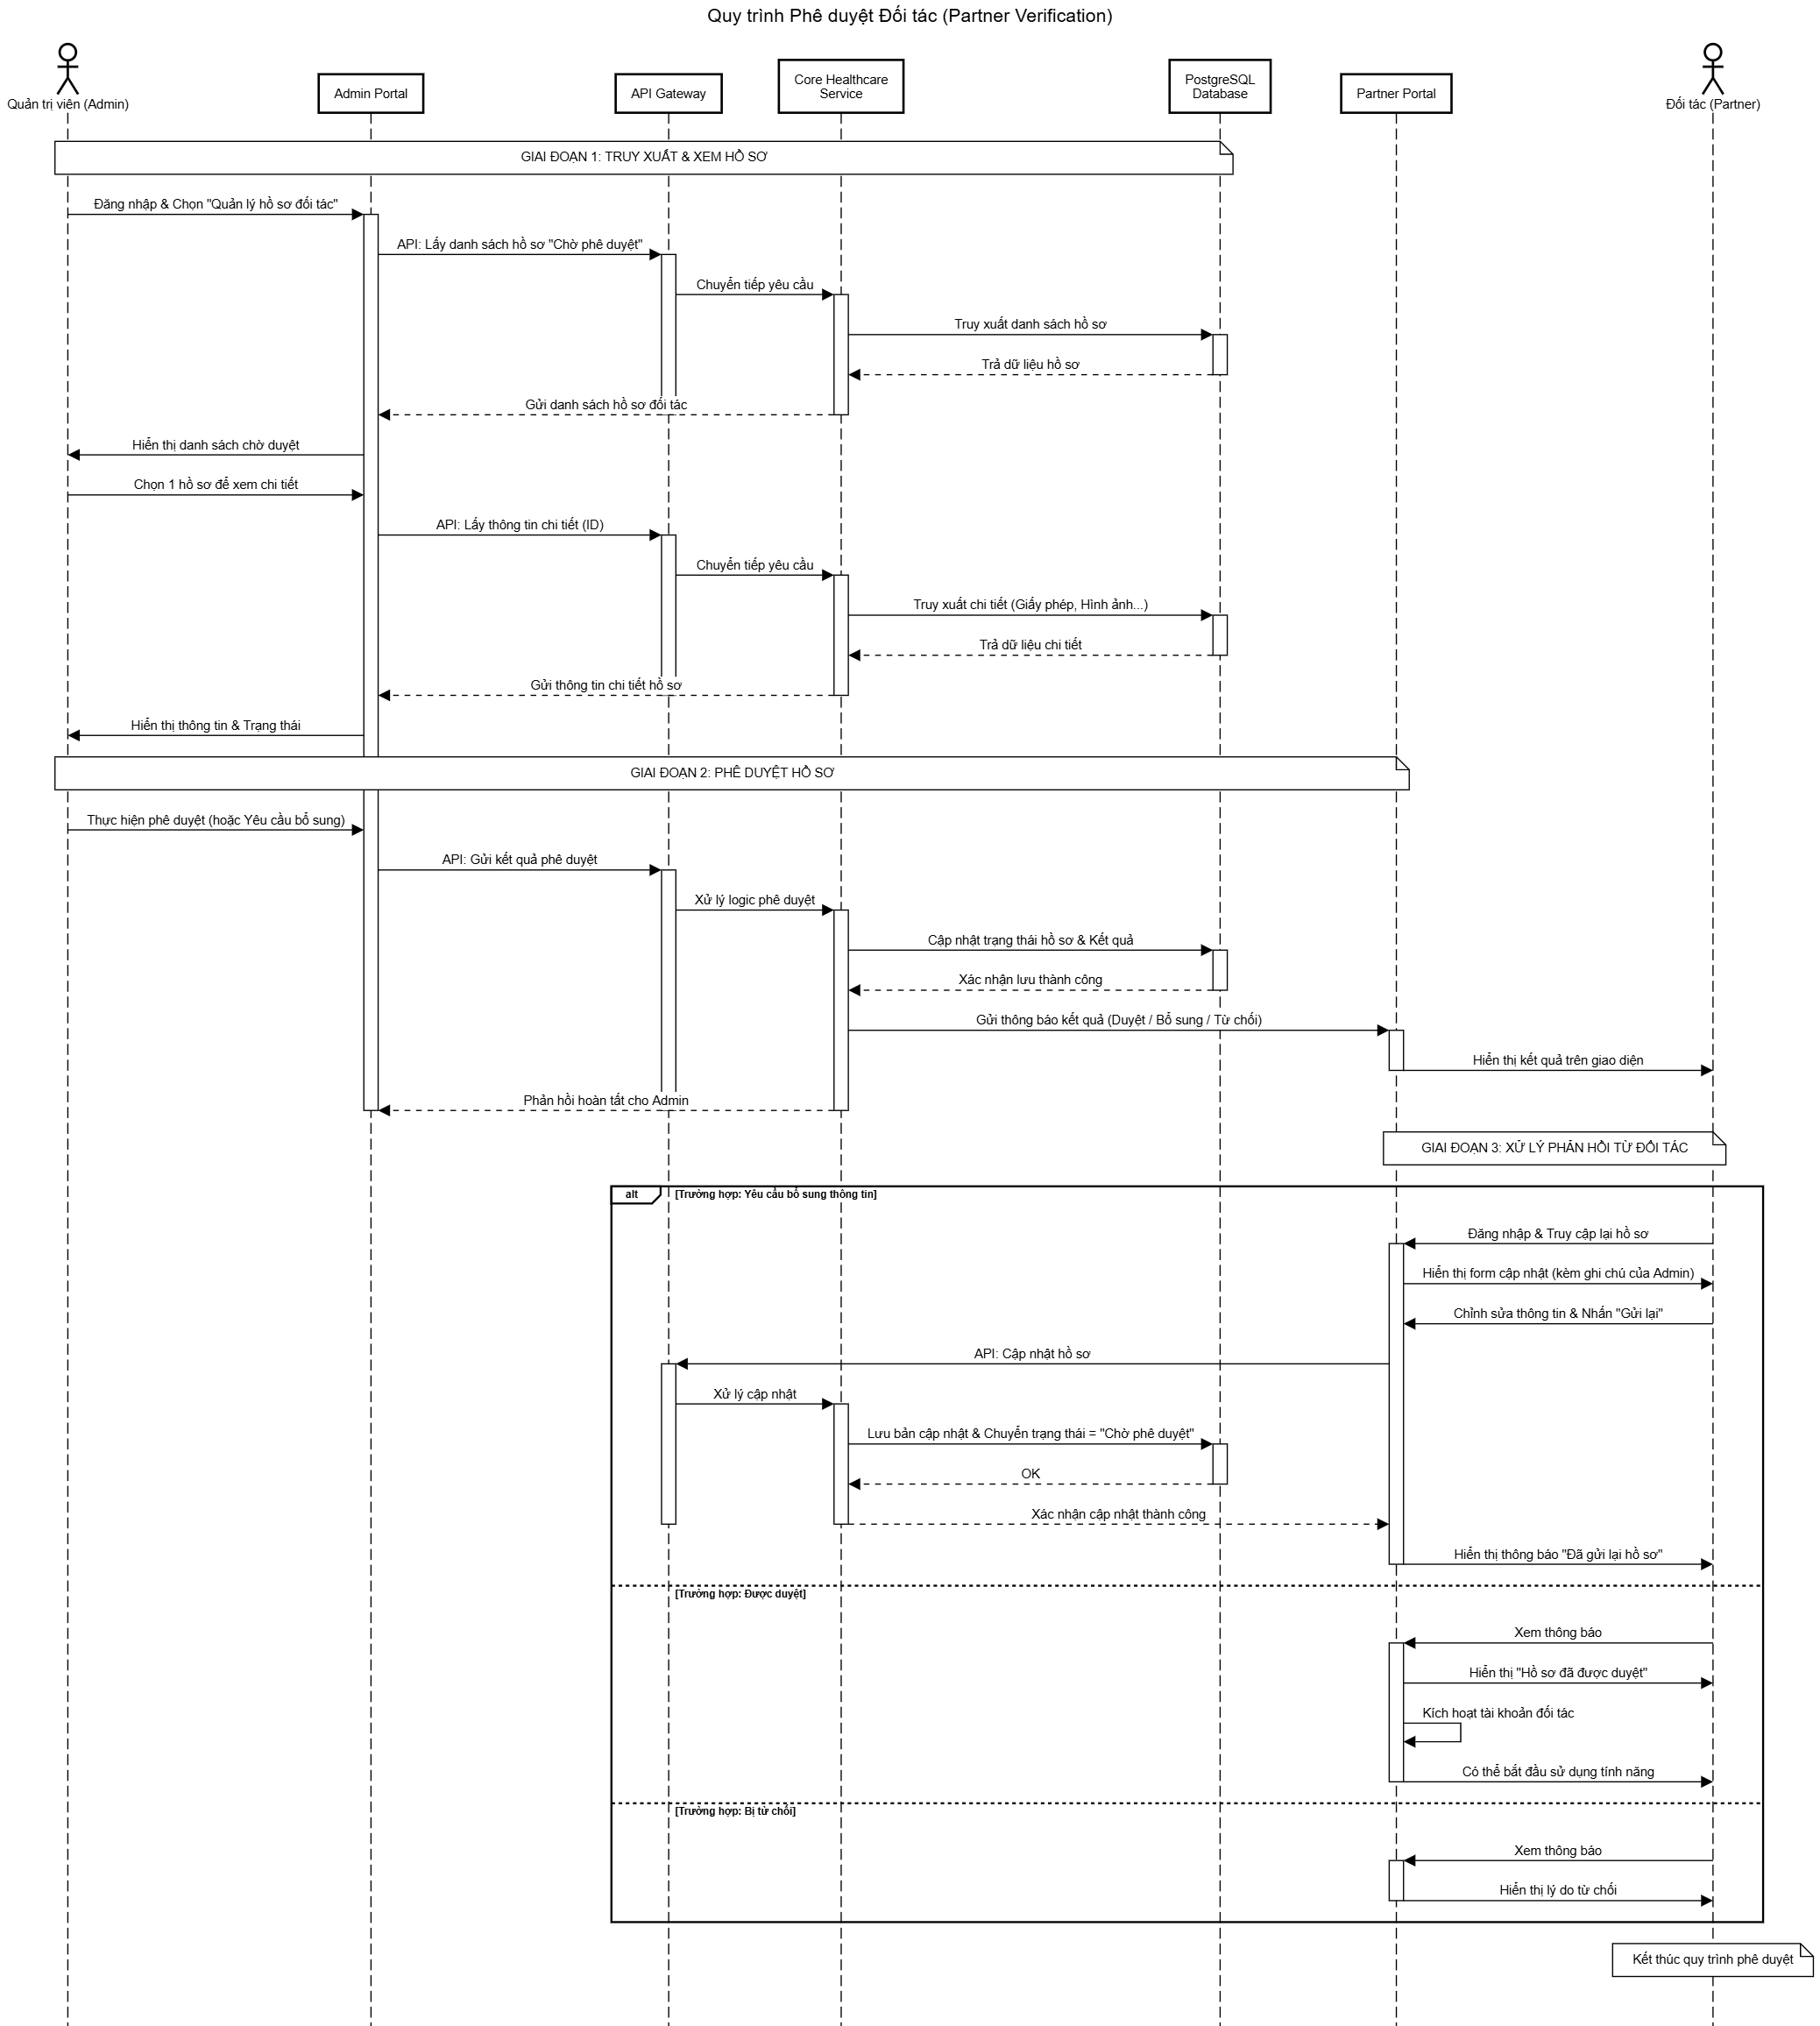
\includegraphics[width=0.8\textwidth]{Images/sequences/4.2.8.png}
    \vspace{10pt}
    
    % Thêm chú thích cho hình ảnh
    \caption{Cổng thông tin Chờ duyệt}
    
    % Đặt nhãn để tham chiếu chéo (cross-reference)
    \label{fig:seq_partner_verification}
\end{figure}
Hình \ref{fig:seq_partner_verification} chi tiết hóa quy trình xác thực và phê duyệt hồ sơ đối tác. Giai đoạn 1 - Truy xuất và xem hồ sơ: Admin và Quản lý viên đăng nhập vào Admin Portal để lấy danh sách hồ sơ "Chờ phê duyệt" từ API Gateway. Hệ thống truy xuất thông tin từ Core Healthcare Service và hiển thị danh sách chi tiết. Admin có thể chọn 1 hồ sơ để xem chi tiết (ID, giấy phép, hình ảnh...). Giai đoạn 2 - Phê duyệt hồ sơ: Admin thực hiện phê duyệt bằng cách gọi API với logic phê duyệt, hệ thống xác nhận lại thông tin và cập nhật trạng thái thành "Đã duyệt" (Approved) hoặc "Từ chối" trong database, sau đó gửi thông báo cho đối tác và phản hồi kết quả cho Admin. Giai đoạn 3 - Xử lý phản hồi từ đối tác: Trong trường hợp bị từ chối, đối tác có thể xem thông báo, kiểm tra lý do từ chối, chỉnh sửa thông tin và nộp lại hồ sơ. Admin có thể cập nhật hồ sơ, lưu bản cáo và chuyển trạng thái thành "Đang xem xét". Toàn bộ quy trình giúp đảm bảo tính minh bạch và truy vết trong việc phê duyệt đối tác.

\subsection{Quản lý Lịch hẹn (Booking Dashboard)}
\begin{figure}[H]
    % Căn giữa hình ảnh
    \centering
    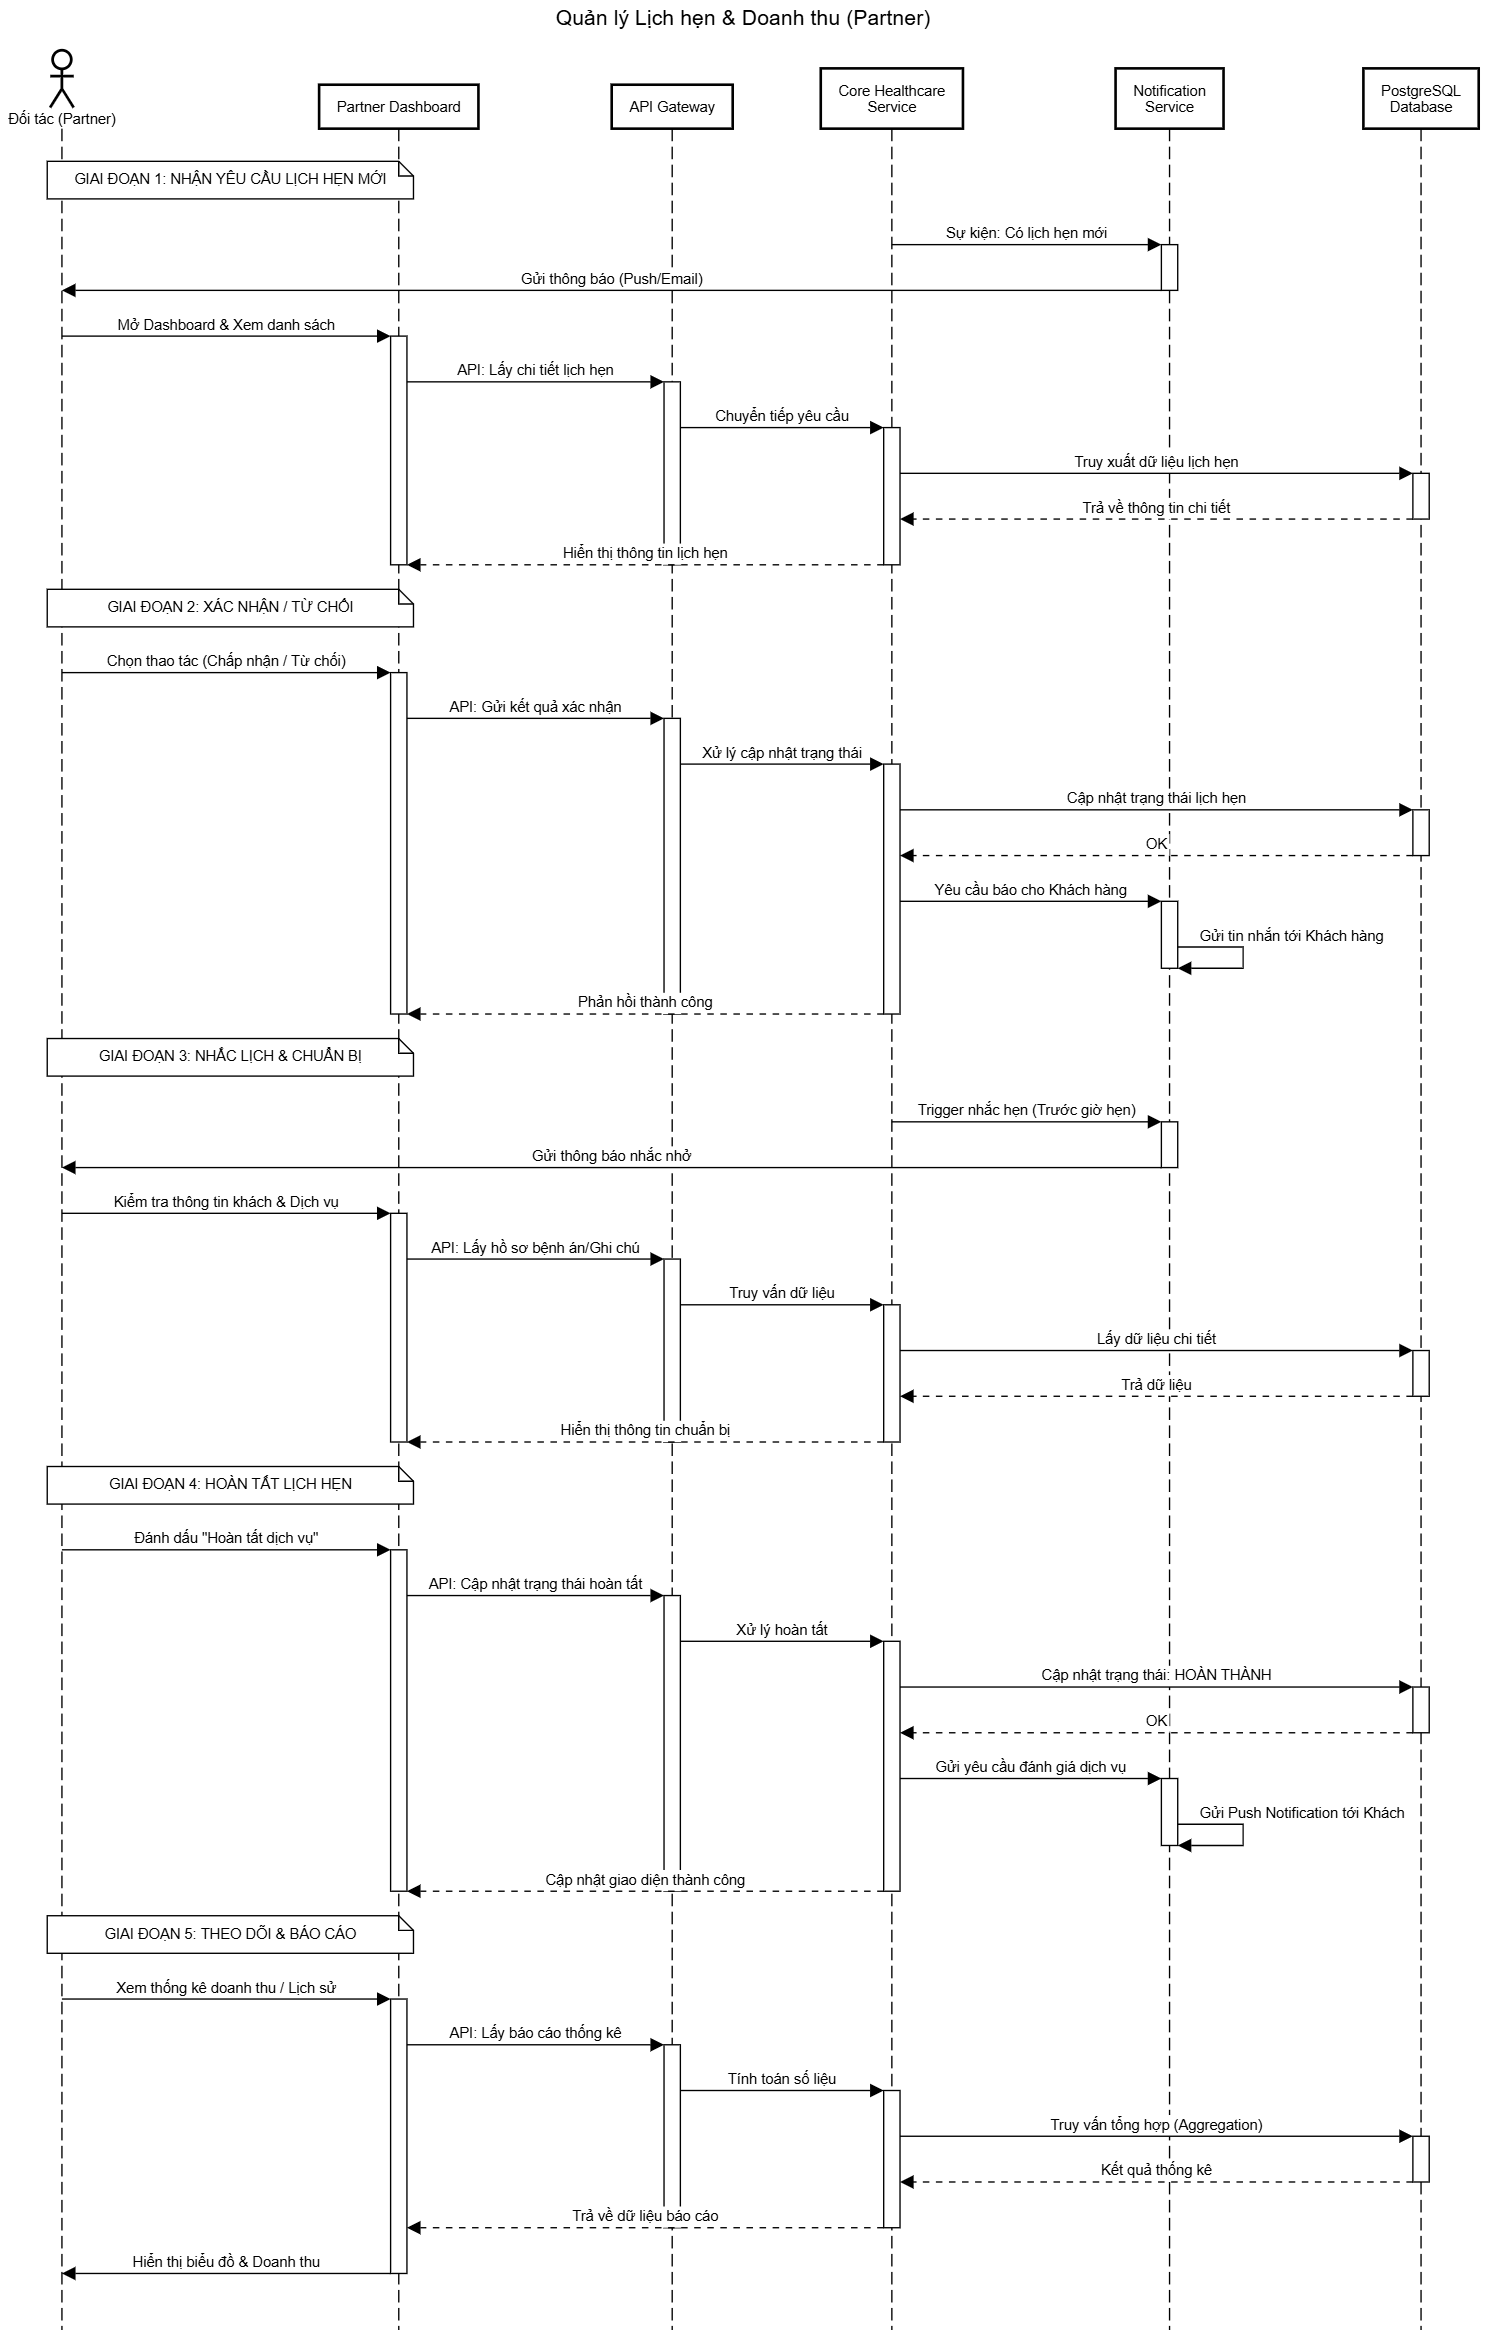
\includegraphics[width=0.8\textwidth]{Images/sequences/4.2.9.png}
    \vspace{10pt}
    
    % Thêm chú thích cho hình ảnh
    \caption{Quản lý lịch hẹn}
    
    % Đặt nhãn để tham chiếu chéo (cross-reference)
    \label{fig:Booking_dashboard}
\end{figure}
Hình \ref{fig:Booking_dashboard} mô tả quy trình quản lý lịch hẹn từ phía đối tác thông qua Partner Dashboard. Quy trình bao gồm 5 giai đoạn chính: Giai đoạn 1 - Nhận yêu cầu lịch hẹn mới: Khi có lịch hẹn mới, hệ thống kích hoạt sự kiện và gửi thông báo PushEmail đến đối tác. Đối tác mở Dashboard và xem danh sách lịch hẹn, hệ thống truy xuất dữ liệu từ Core Healthcare Service và hiển thị thông tin chi tiết. Giai đoạn 2 - Xác nhận/Từ chối: Đối tác có thể chọn xác nhận hoặc từ chối lịch hẹn. Nếu xác nhận, hệ thống cập nhật trạng thái thành CONFIRMED, gửi tin nhắn cho khách hàng và yêu cầu gửi notification. Nếu từ chối, lý do từ chối được lưu và thông báo gửi đến người dùng. Giai đoạn 3 - Nhắc lịch và chuẩn bị: Hệ thống tự động trigger nhắc nhở trước giờ hẹn, gửi thông tin chi tiết về bệnh án/chi chú đến đối tác và lấy dữ liệu chi tiết. Giai đoạn 4 - Hoàn tất lịch hẹn: Sau khi hoàn thành dịch vụ, đối tác cập nhật trạng thái thành HOÀN THÀNH, ghi chú kết quả, hệ thống lưu trạng thái vào database và gửi yêu cầu đánh giá cho khách hàng. Giai đoạn 5 - Theo dõi và báo cáo: Đối tác có thể xem thống kê doanh thu, lịch sử hoàn tất, tính toán số liệu tổng hợp và hiển thị dashboard báo cáo đầy đủ.

\subsection{Quản lý Dịch vụ (Service Management)}
\begin{figure}[H]
    % Căn giữa hình ảnh
    \centering
    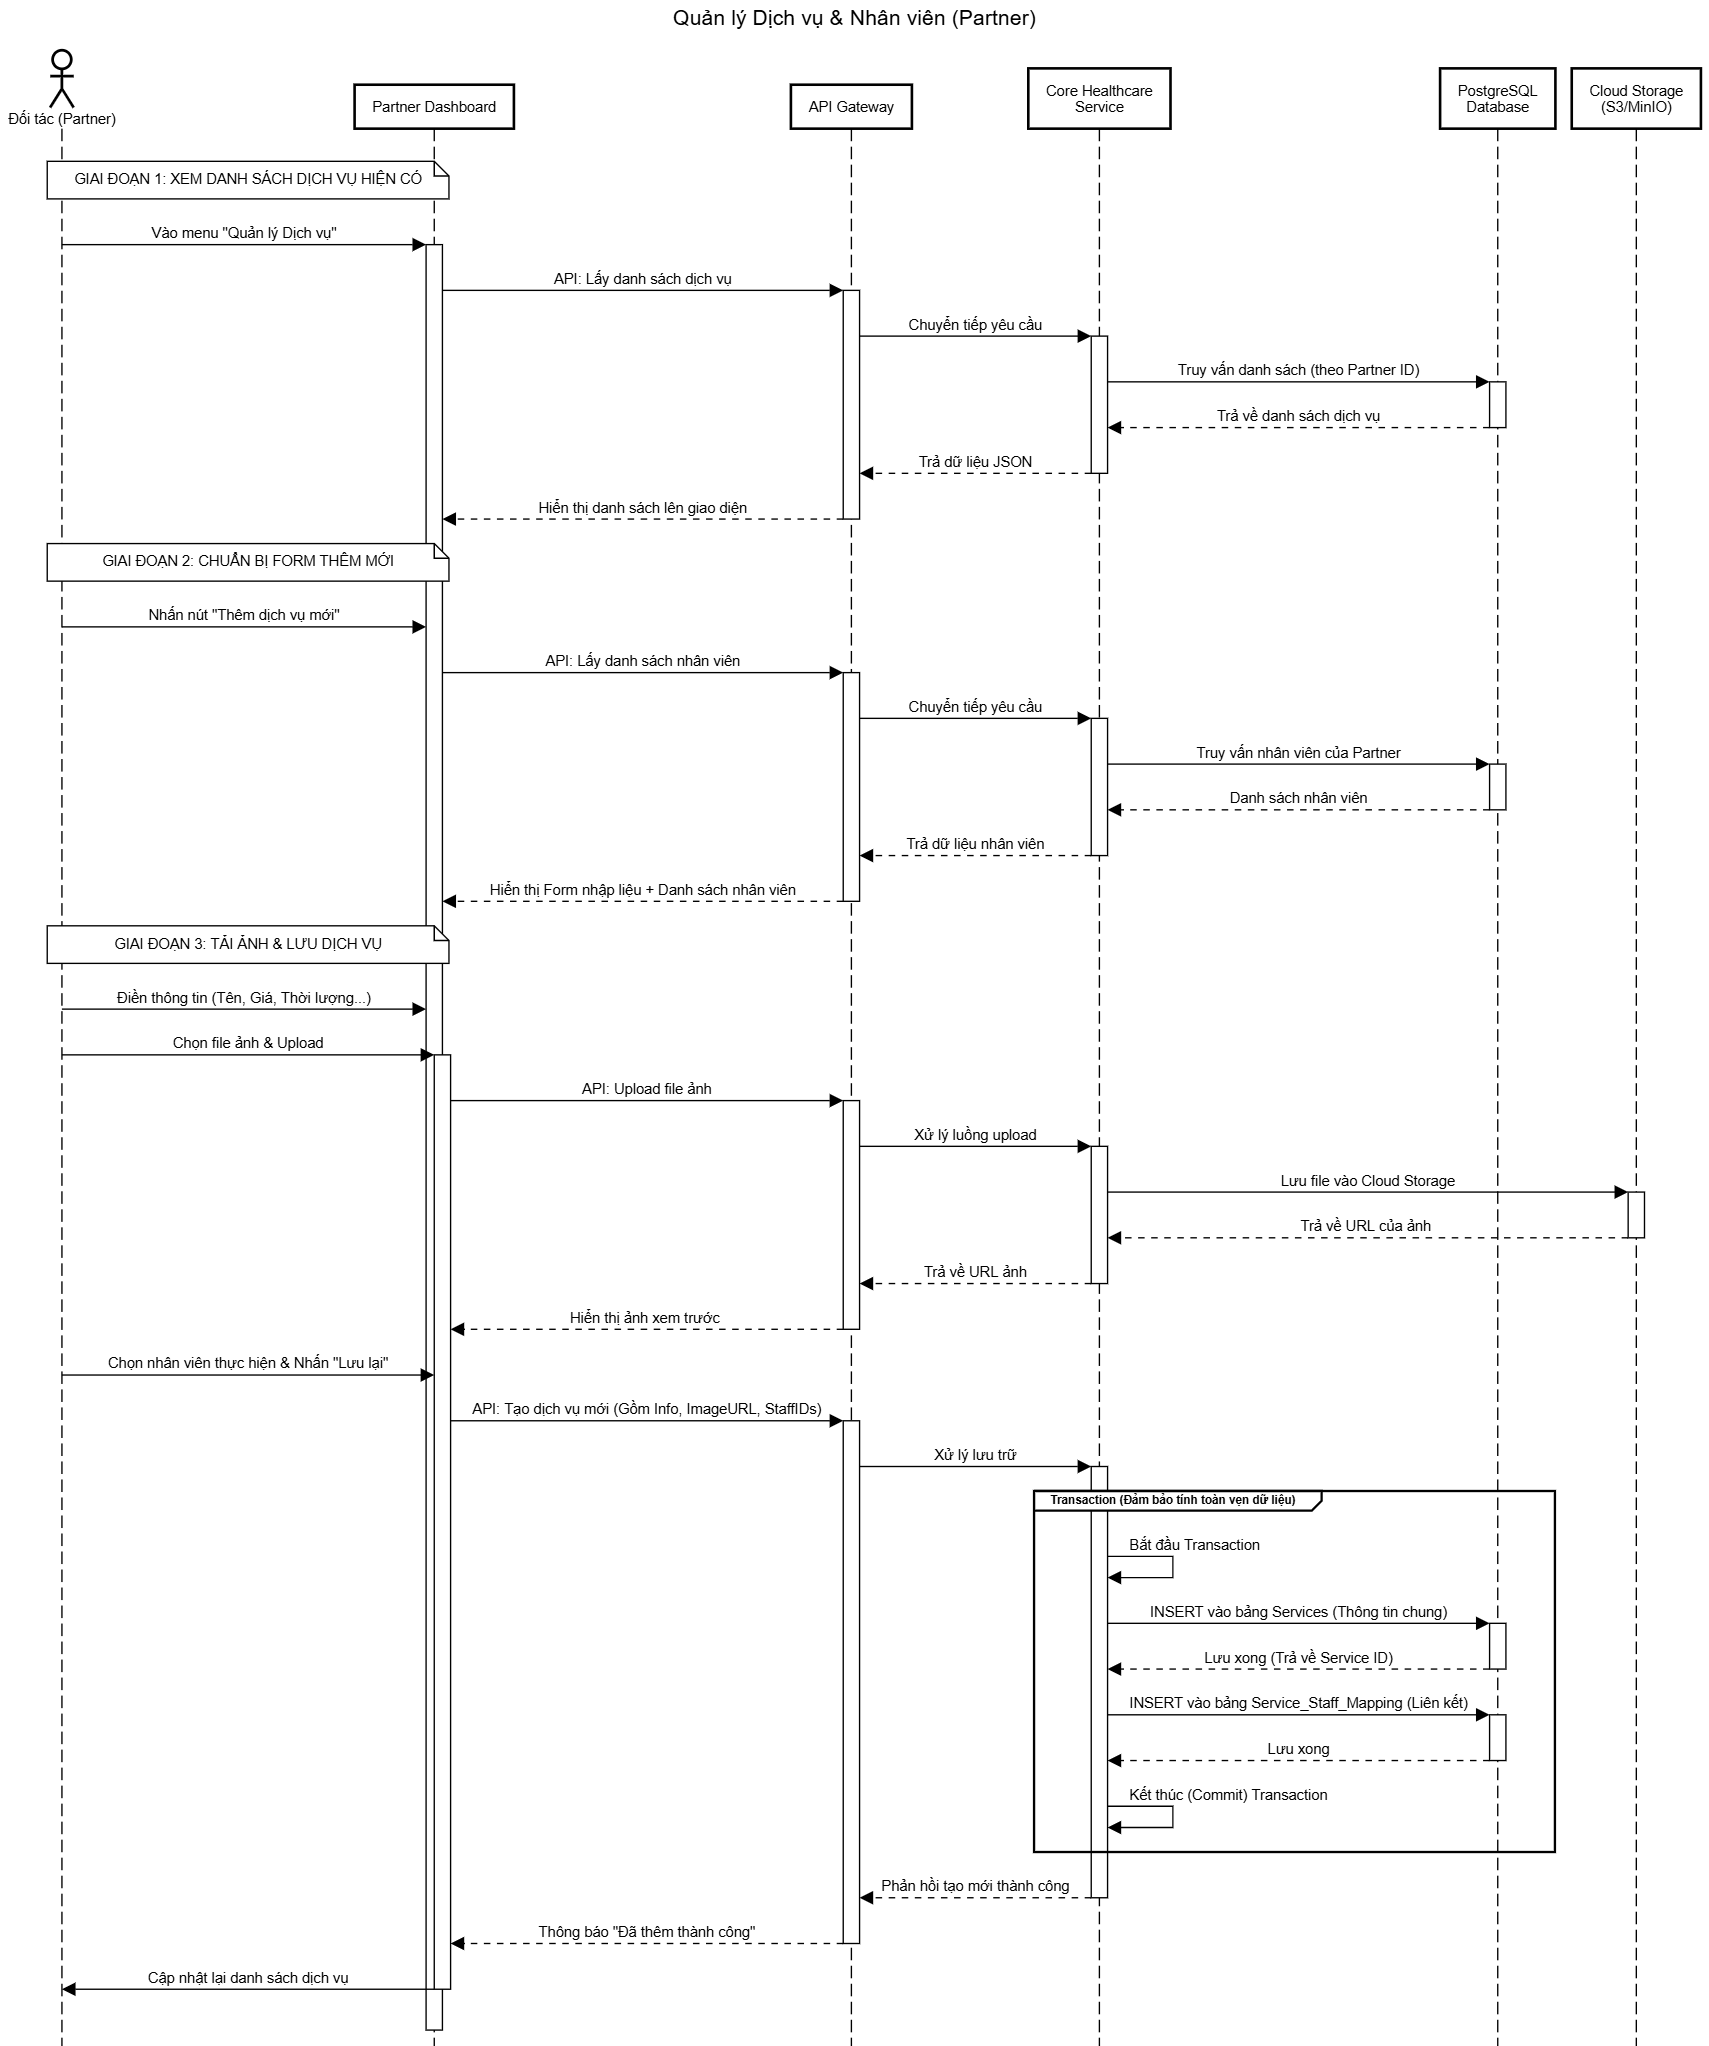
\includegraphics[width=0.8\textwidth]{Images/sequences/4.2.10.png}
    \vspace{10pt}
    
    % Thêm chú thích cho hình ảnh
    \caption{Quản lý Dịch vụ (Service Management)}
    
    % Đặt nhãn để tham chiếu chéo (cross-reference)
    \label{fig:seq_service_management}
\end{figure}
Hình \ref{fig:seq_service_management} thể hiện quy trình quản lý dịch vụ y tế của đối tác qua Partner Dashboard, bao gồm 3 giai đoạn chính. Giai đoạn 1 - Xem danh sách dịch vụ hiện có: Đối tác vào menu "Quản lý Dịch vụ", hệ thống gọi API để lấy danh sách dịch vụ theo Partner ID từ Core Healthcare Service, truy vấn database và trả về dữ liệu dạng JSON, sau đó hiển thị danh sách dịch vụ trên giao diện. Giai đoạn 2 - Chuẩn bị form thêm mới: Khi đối tác nhấn nút "Thêm dịch vụ mới", hệ thống gọi API để lấy danh sách nhân viên của Partner, truy vấn thông tin nhân viên từ database và hiển thị form nhập liệu với danh sách nhân viên. Giai đoạn 3 - Tải ảnh và lưu dịch vụ: Đối tác điền thông tin (tên, giá, thời lượng) và chọn file ảnh để upload. Hệ thống xử lý upload, lưu file vào Cloud Storage (S3/MinIO) và nhận về URL của ảnh. Sau đó, đối tác chọn nhân viên thực hiện và nhấn "Lưu lại", hệ thống tạo dịch vụ mới với thông tin đầy đủ (Tên, Giá, ImageURL, StaffIDs), bắt đầu transaction để đảm bảo tính toàn vẹn dữ liệu, thực hiện INSERT vào bảng Services (Thông tin chung), INSERT vào bảng Service\_Staff\_Mapping (Liên kết nhân viên), commit transaction và lưu hoàn tất. Cuối cùng, hệ thống phản hồi báo thành công và hiển thị danh sách dịch vụ đã cập nhật.

\subsection{Quản lý Nhân viên Phân quyền (Staff Management )}
\begin{figure}[H]
    % Căn giữa hình ảnh
    \centering
    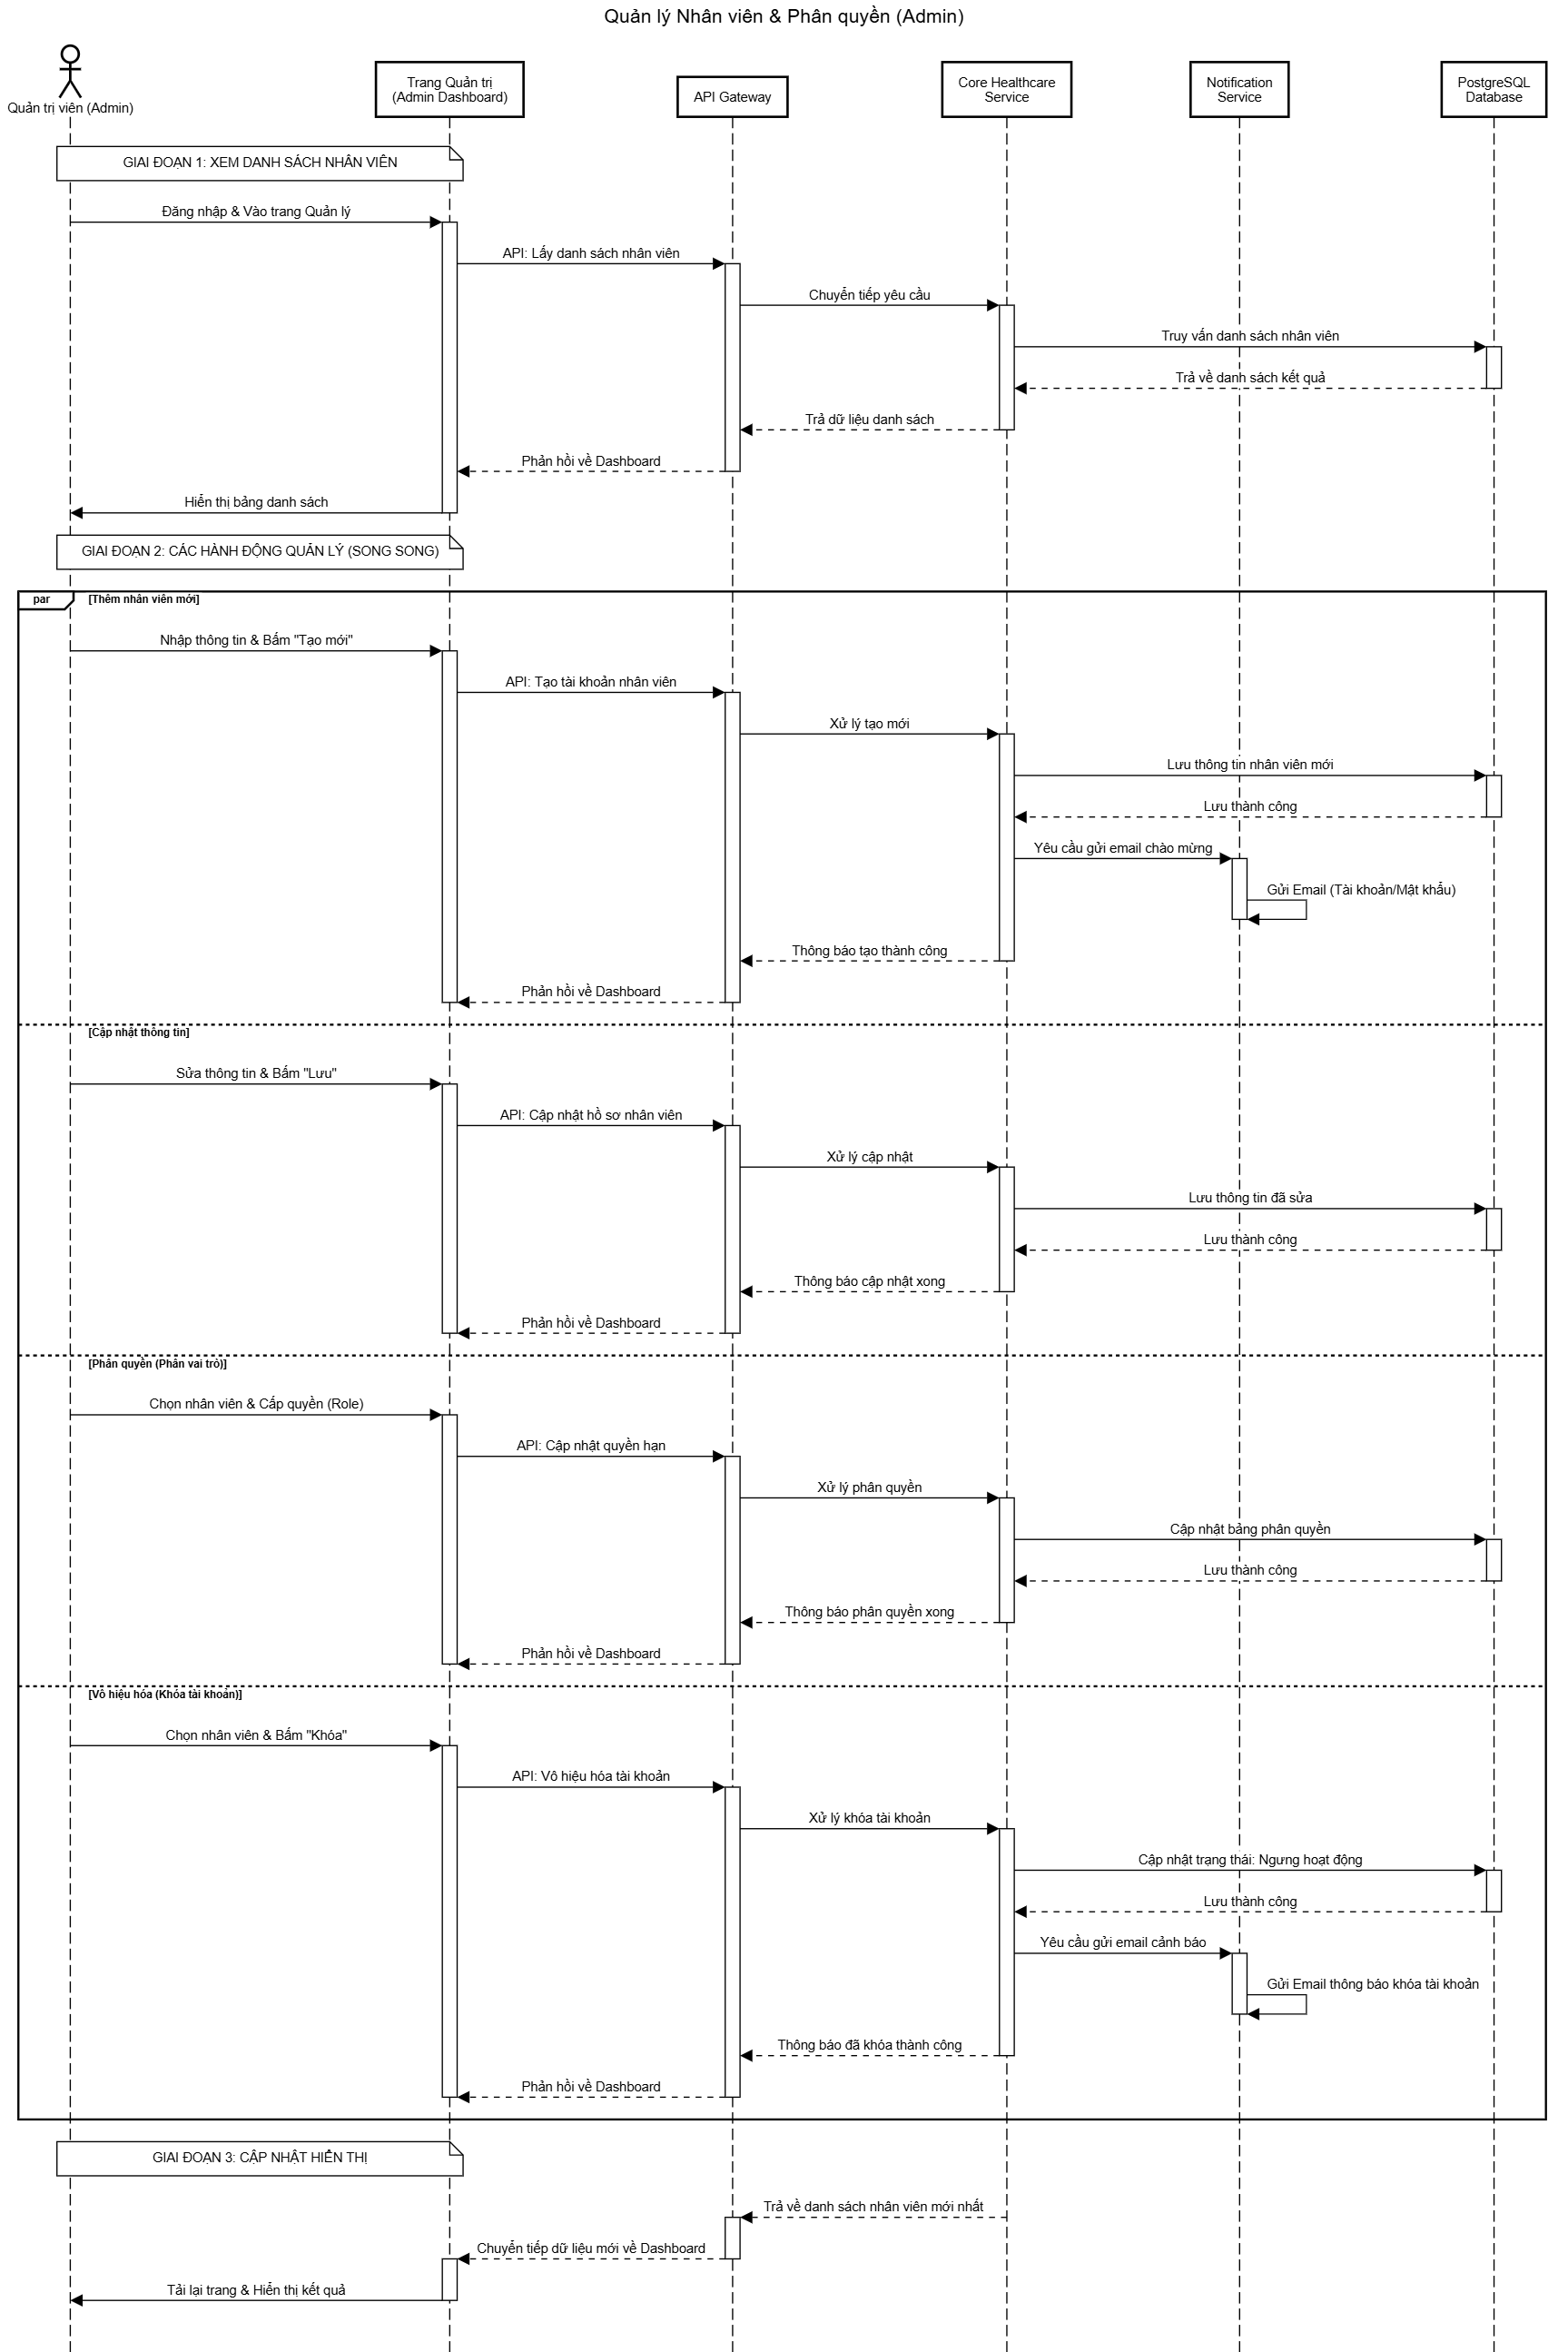
\includegraphics[width=0.8\textwidth]{Images/sequences/4.2.11.png}
    \vspace{10pt}
    
    % Thêm chú thích cho hình ảnh
    \caption{Quản lý Nhân viên (Staff Management)}
    
    % Đặt nhãn để tham chiếu chéo (cross-reference)
    \label{fig:seq_staff_management}
\end{figure}
Hình \ref{fig:seq_staff_management} mô tả chi tiết quy trình quản lý nhân viên và phân quyền trong hệ thống đối tác. Quy trình được chia làm 3 giai đoạn chính. Giai đoạn 1 - Xem danh sách nhân viên: Đối tác đăng nhập và vào menu "Quản lý Nhân viên", hệ thống gọi API Gateway để lấy danh sách nhân viên thuộc Partner, Core Healthcare Service truy vấn database theo Partner ID, trả về danh sách dưới dạng JSON và hiển thị trên giao diện. Giai đoạn 2 - Chuẩn bị form thêm mới: Khi đối tác nhấn "Thêm nhân viên mới", hệ thống gọi API để lấy danh sách nhân viên của đối tác, truy vấn thông tin từ Core Healthcare Service và hiển thị form với danh sách nhân viên có thể được thêm vào. Giai đoạn 3 - Tải ảnh và lưu dịch vụ: Đối tác điền thông tin nhân viên (tên, chức danh, kinh nghiệm) và upload file ảnh. API xử lý upload, lưu file vào Cloud Storage (S3MinIO) và nhận về URL ảnh. Đối tác sau đó chọn nhân viên và nhấn "Lưu lại", hệ thống tạo hồ sơ mới với các thông tin đầy đủ, khởi động transaction bảo toàn dữ liệu, thực hiện INSERT thông tin vào database, commit transaction và phản hồi thông báo tạo thành công. Cuối cùng, danh sách nhân viên được làm mới để hiển thị nhân viên vừa thêm.


% \subsection{Tạo và Quản lý Khuyến mãi (Promotions Management)}

% \subsection{Báo cáo Phân tích Kinh doanh (Business Analytics Reporting)}


% \subsection{Quản lý Đánh giá Báo cáo (Review Report Moderation)}

% \subsection{Quản lý Tài chính Toàn hệ thống (System-wide Financial Management)}

% \subsection{Quản lý Mã giảm giá Chiến dịch Marketing (Voucher Campaign Management)}

% \subsection{Trung tâm Hỗ trợ Ticket (Support Center Ticketing System)}

%%%%%%%%%%%%%%%%%%%%%%





%%%%%%%%%%%%%%%%%%%%%%%



%%%%%%%%%%%%%%%%%%%%%%%%
\section{Sơ đồ Activity (Activity Diagram)}
Phần này mô tả chi tiết các luồng quy trình nghiệp vụ chính của hệ thống thông qua các sơ đồ hoạt động (activity diagram), thể hiện sự tương tác giữa các tác nhân (Người dùng, Đối tác, Admin) và các thành phần hệ thống (Ứng dụng Client, Máy chủ, Database).
\newpage

\subsection{Luồng Onboarding và Cá nhân hóa Người dùng}
Sơ đồ này mô tả quy trình từ lúc người dùng mở ứng dụng lần đầu, thực hiện đăng ký tài khoản (qua Email hoặc Google/Facebook), cho đến khi hoàn tất khảo sát cá nhân hóa. Dữ liệu khảo sát được máy chủ/AI phân tích để tạo hồ sơ người dùng và đưa ra các gợi ý dịch vụ phù hợp ngay khi onboarding.

\begin{figure}[H]
    % Căn giữa hình ảnh
    \centering
    % Sử dụng width=1\textwidth để hình ảnh vừa với chiều rộng trang
    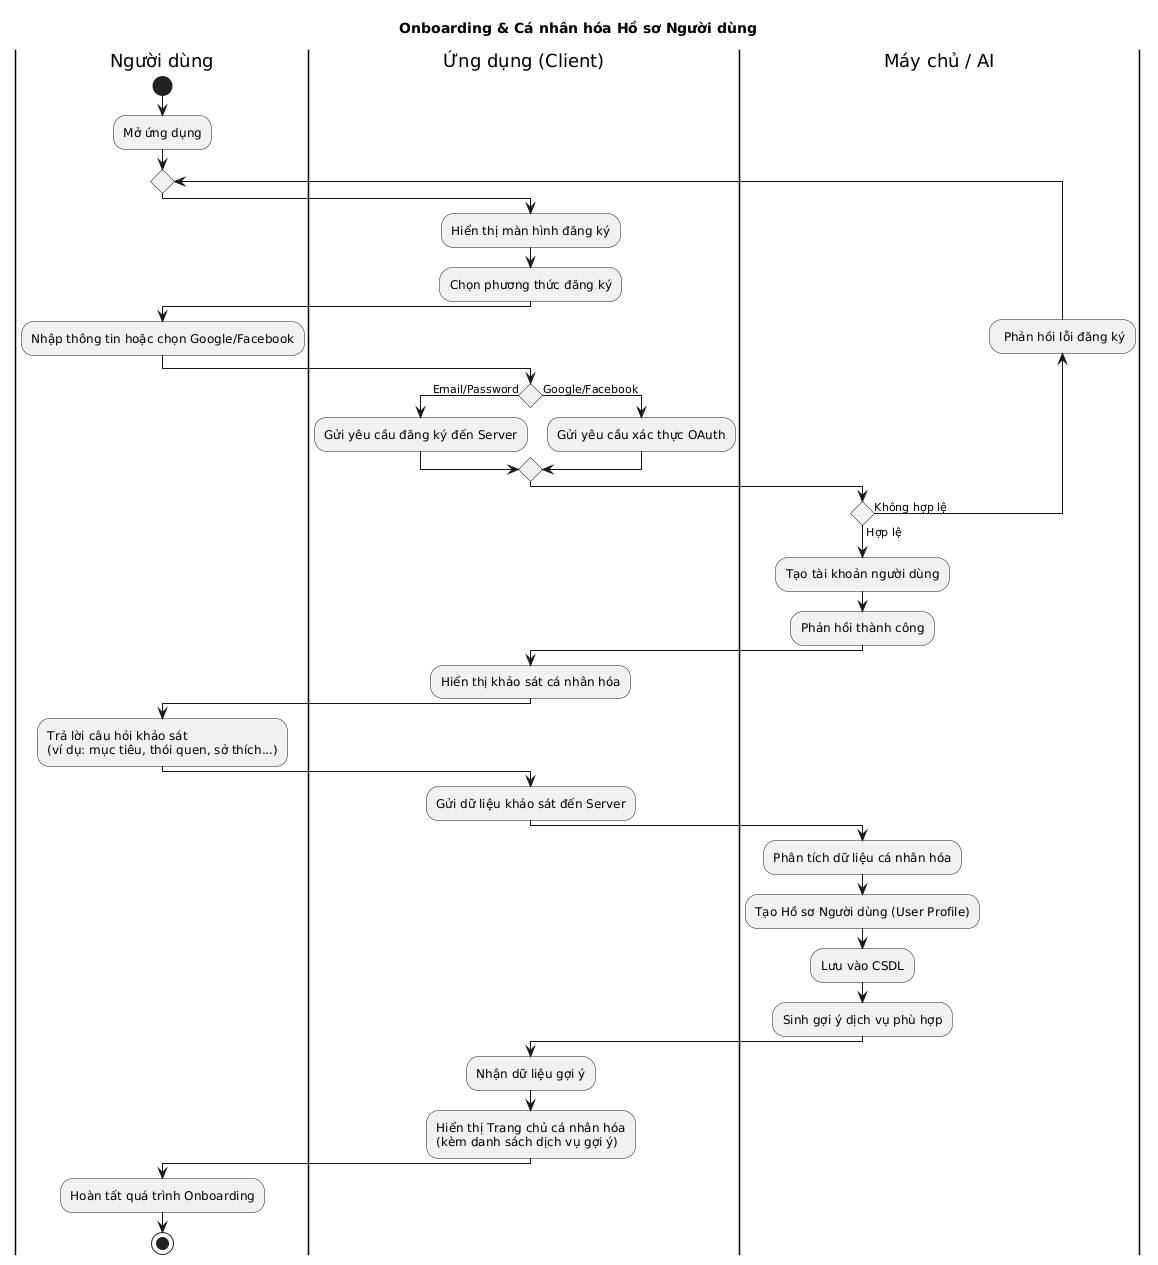
\includegraphics[width=0.8\textwidth]{Images/Activity/4.5.1.png}
    \vspace{10pt}

    % Thêm chú thích cho hình ảnh
   \caption{Sơ đồ hoạt động Onboarding \& Cá nhân hóa Hồ sơ Người dùng}

    % Đặt nhãn để tham chiếu chéo (cross-reference)
    \label{fig:activity_user_onboarding}
\end{figure}

\subsection{Luồng Chatbot AI Tư vấn \& Gợi ý Dịch vụ}
Sơ đồ này mô tả cách người dùng tương tác với Chatbot AI. Khi người dùng nhập yêu cầu tư vấn, máy chủ/AI sẽ sử dụng NLP để phân tích ngữ nghĩa, tách ý định (intent) và thực thể (entities). Dựa trên hồ sơ người dùng và dữ liệu đầu vào, hệ thống gợi ý (Recommender System) sẽ tính toán và trả về danh sách các dịch vụ phù hợp nhất.

\begin{figure}[H]
    % Căn giữa hình ảnh
    \centering
    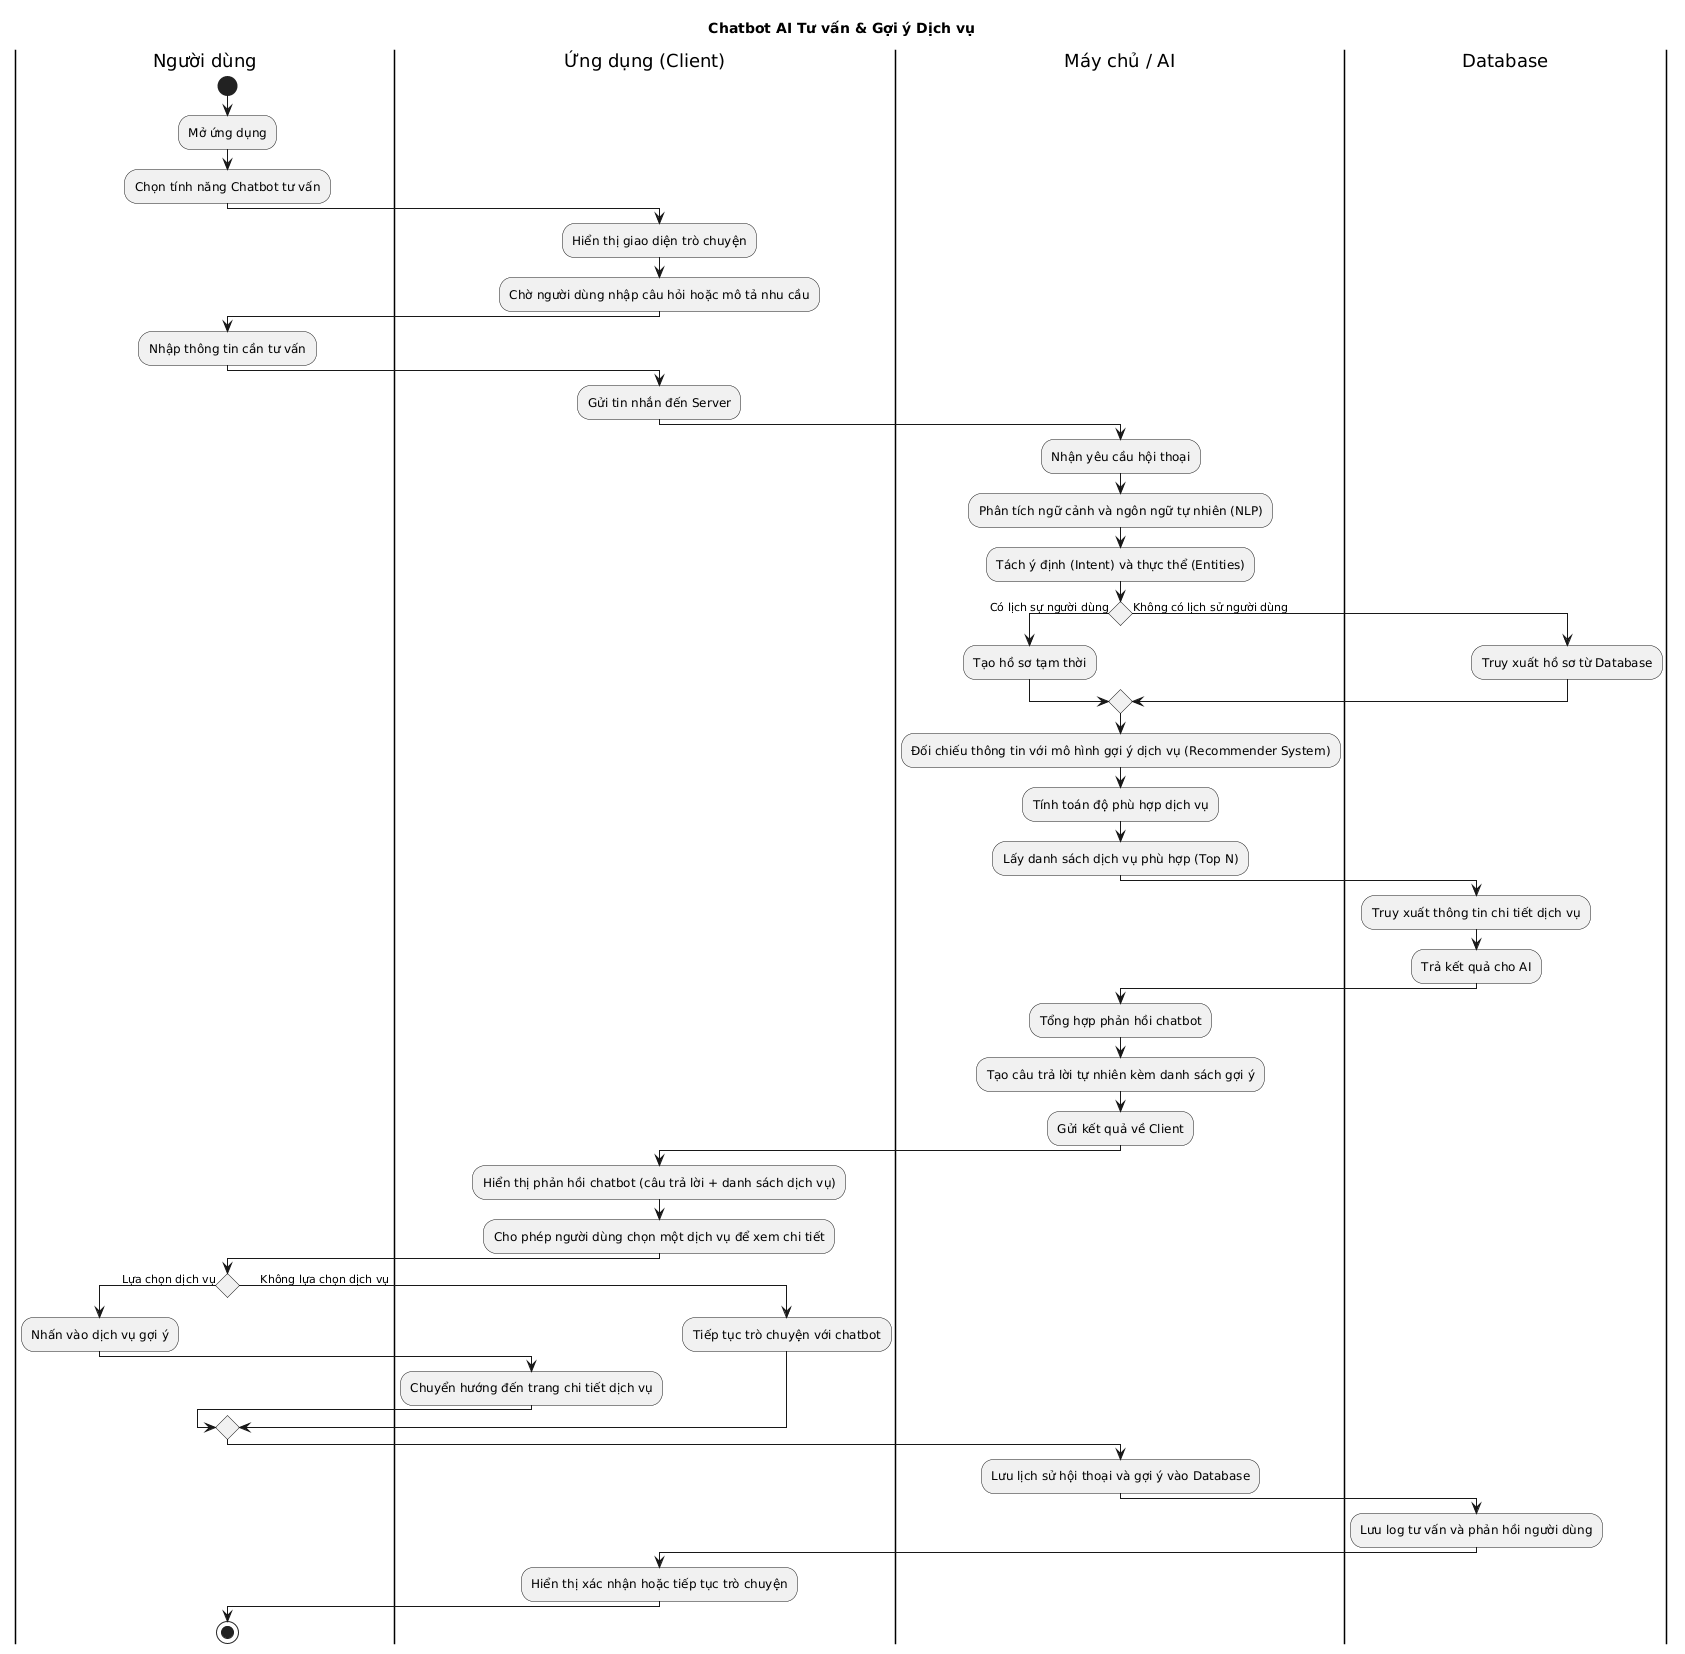
\includegraphics[width=0.8\textwidth]{Images/Activity/4.5.2.png}
    \vspace{10pt}

    % Thêm chú thích cho hình ảnh
    \caption{Sơ đồ hoạt động Chatbot AI Tư vấn \& Gợi ý Dịch vụ}

    % Đặt nhãn để tham chiếu chéo (cross-reference)
    \label{fig:activity_ai_chatbot}
\end{figure}

\subsection{Quy trình Đăng ký Đối tác (Partner Registration)}
Mô tả luồng đăng ký dành cho đối tác (Partner) mới. Đối tác truy cập Partner Portal, điền form đăng ký (thông tin cơ bản, dịch vụ, giấy phép kinh doanh...). Máy chủ tiếp nhận, kiểm tra tính hợp lệ ban đầu (email, SĐT) và lưu hồ sơ vào cơ sở dữ liệu với trạng thái "Chờ phê duyệt".

\begin{figure}[H]
    % Căn giữa hình ảnh
    \centering
    % Lưu ý: Tên file gốc của bạn là 'partner_registation.png' (sai chính tả 'registration')
    % Hãy đảm bảo tên file trong \includegraphics khớp với tên file bạn đã lưu.
    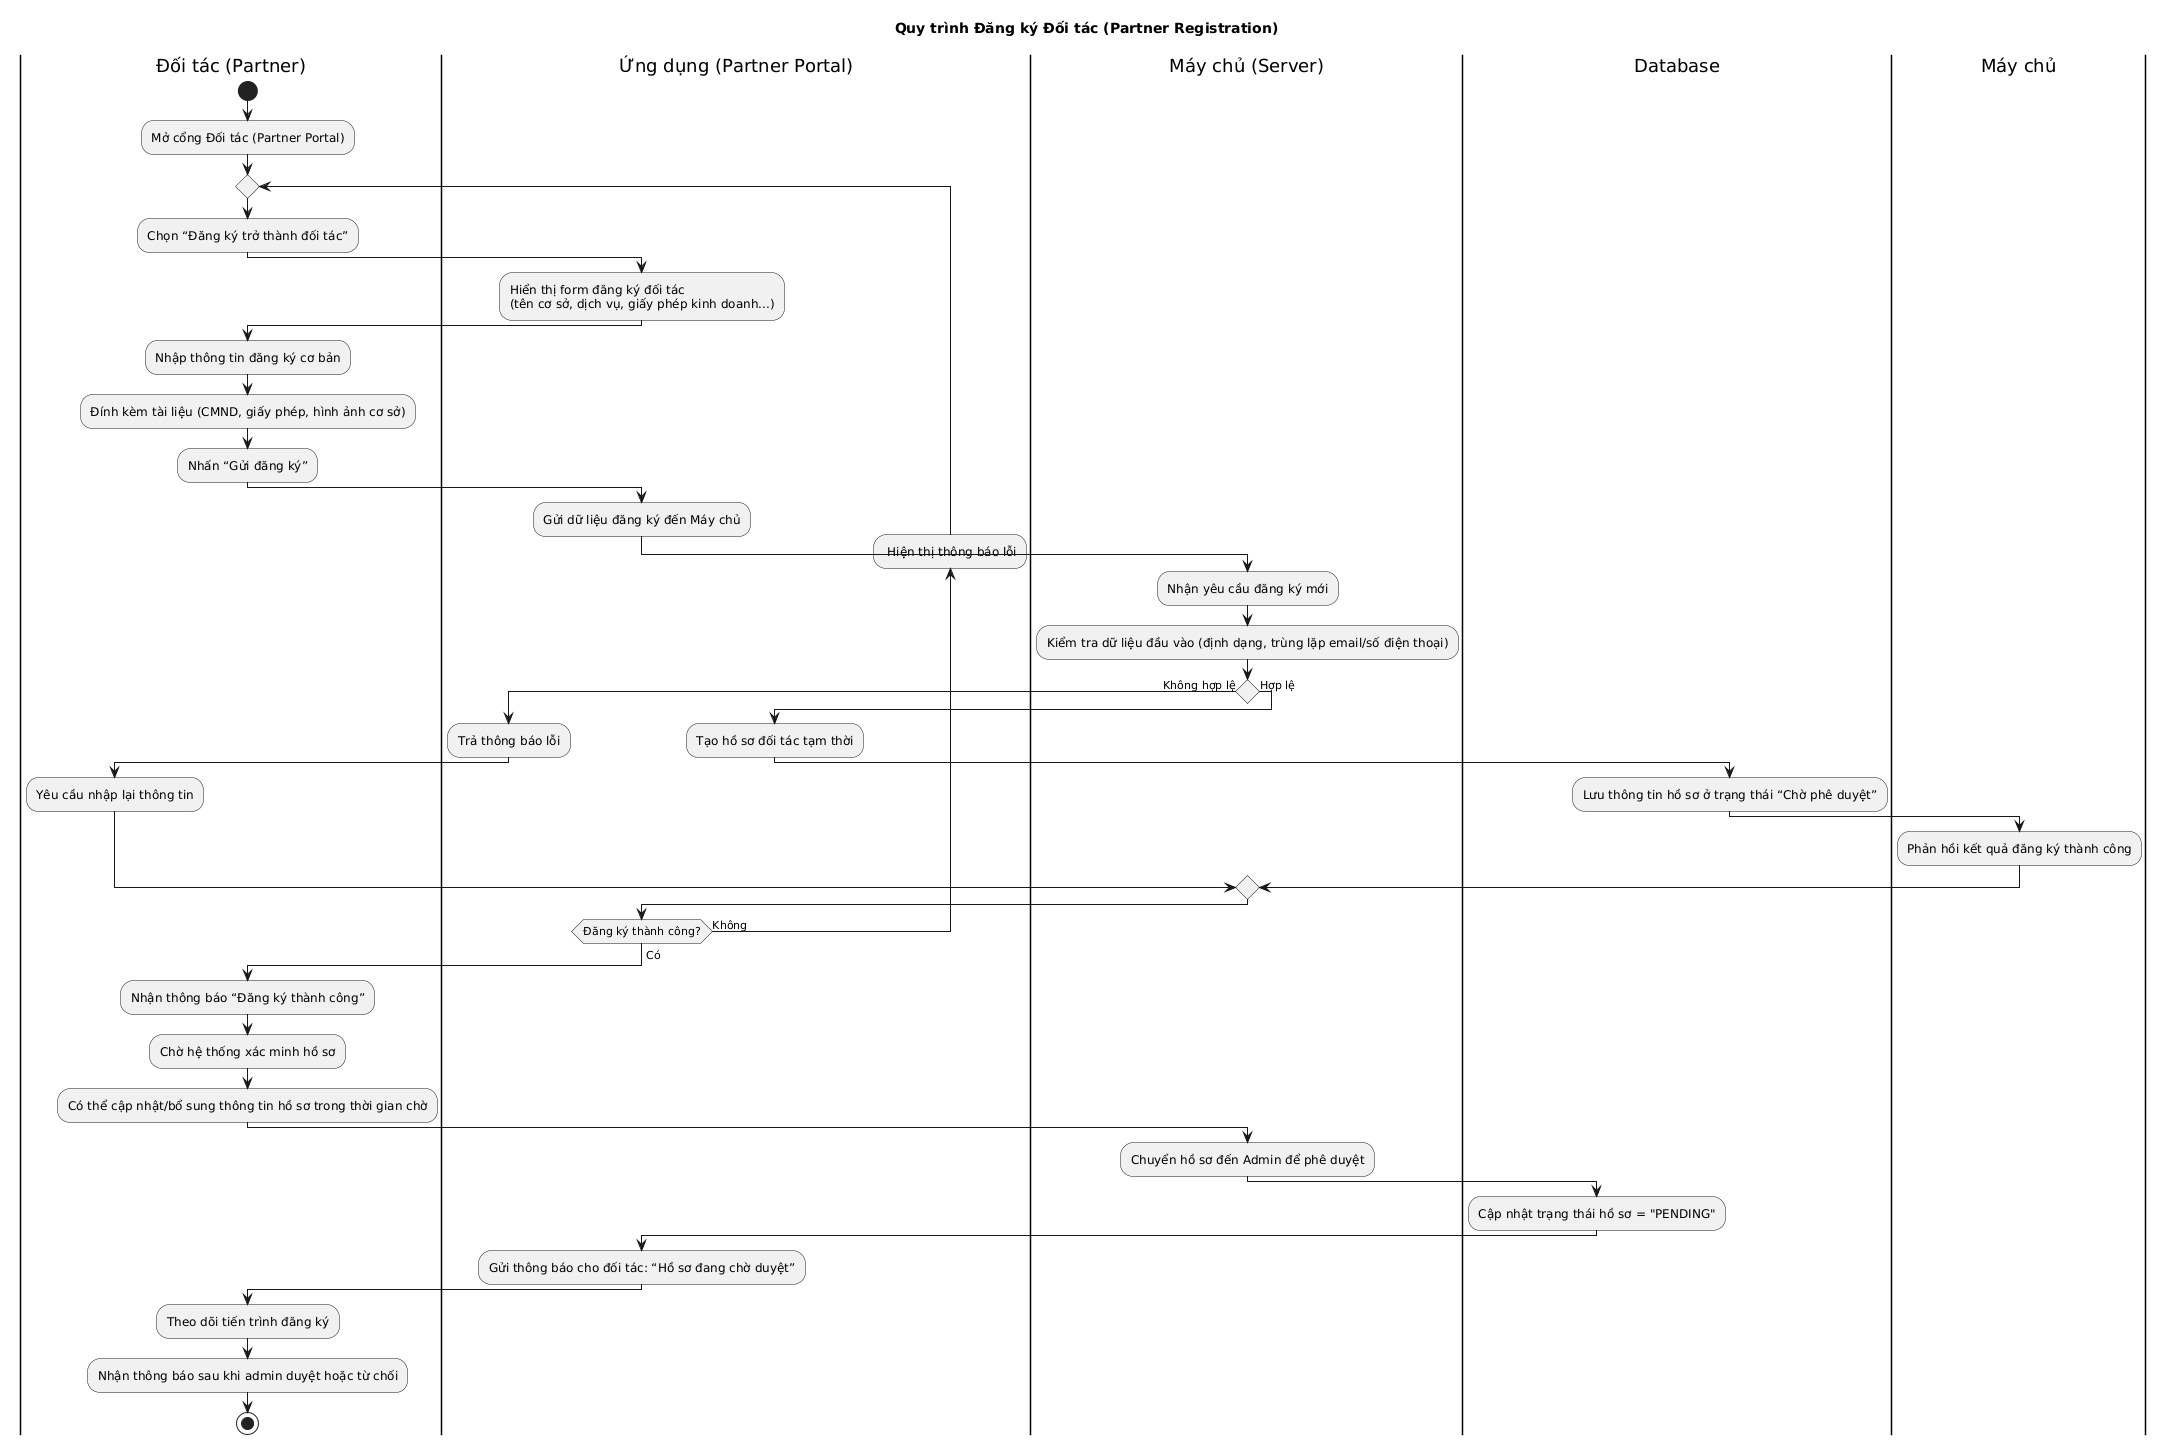
\includegraphics[width=0.8\textwidth]{Images/Activity/4.5.4.png}
    \vspace{10pt}

    % Thêm chú thích cho hình ảnh
    \caption{Sơ đồ hoạt động Quy trình Đăng ký Đối tác}

    % Đặt nhãn để tham chiếu chéo (cross-reference)
    \label{fig:activity_partner_registration}
\end{figure}
\subsection{Luồng Đặt lịch, Thanh toán và Đánh giá}
Sơ đồ này thể hiện quy trình nghiệp vụ lõi của người dùng: bắt đầu từ việc tìm kiếm và chọn dịch vụ, xem chi tiết, chọn lịch trống (ngày, giờ, nhân viên), và xác nhận đặt lịch. Sau đó, người dùng thực hiện thanh toán. Khi dịch vụ hoàn tất, người dùng nhận thông báo và được mời nhập đánh giá (rating \& feedback) cho dịch vụ.

\begin{figure}[H]
    % Căn giữa hình ảnh
    \centering
    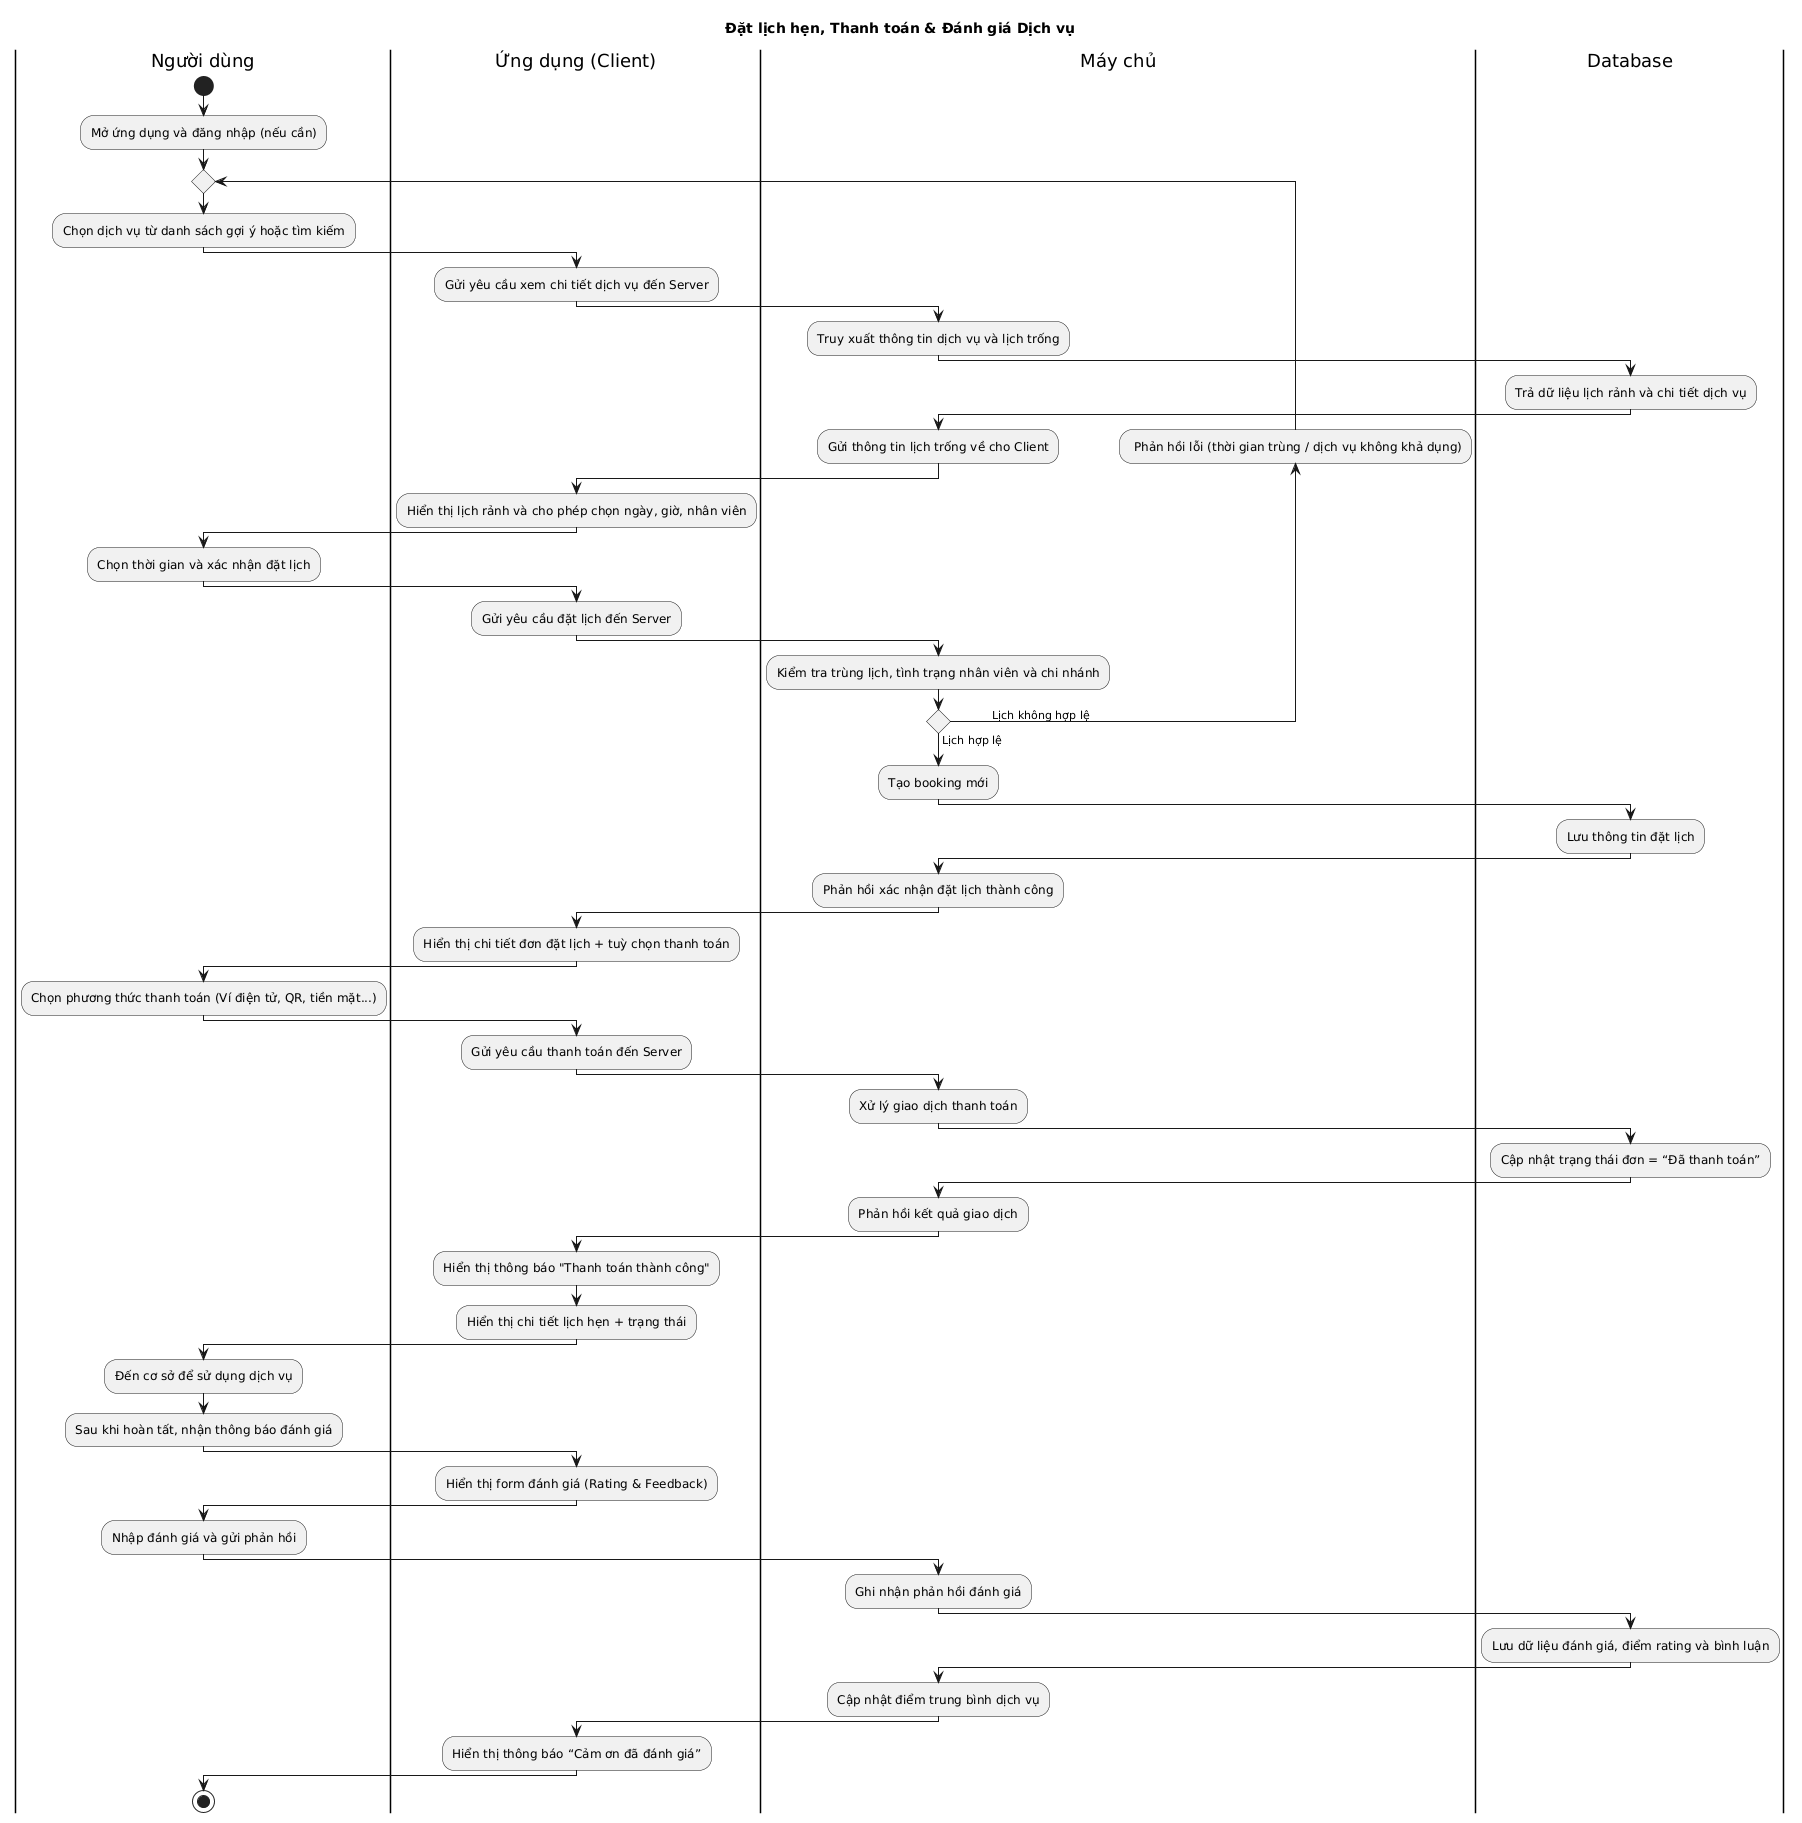
\includegraphics[width=0.8\textwidth]{Images/Activity/4.5.3.png}
    \vspace{10pt}
    
    % Thêm chú thích cho hình ảnh
    \caption{Sơ đồ hoạt động Đặt lịch, Thanh toán \& Đánh giá}

    % Đặt nhãn để tham chiếu chéo (cross-reference)
    \label{fig:activity_booking_payment_rating}
\end{figure}



\subsection{Quy trình Phê duyệt Đối tác (Partner Verification)}
Sơ đồ này mô tả vai trò của Admin trong việc quản lý và xác thực đối tác. Admin đăng nhập, vào mục quản lý đối tác, chọn xem chi tiết các hồ sơ "Chờ phê duyệt". Sau khi xem xét thông tin, Admin thực hiện "Phê duyệt" hoặc "Từ chối". Kết quả được thông báo đến Partner Portal. Nếu bị từ chối, đối tác có thể cập nhật lại hồ sơ và nộp lại.

\begin{figure}[H]
    % Căn giữa hình ảnh
    \centering
    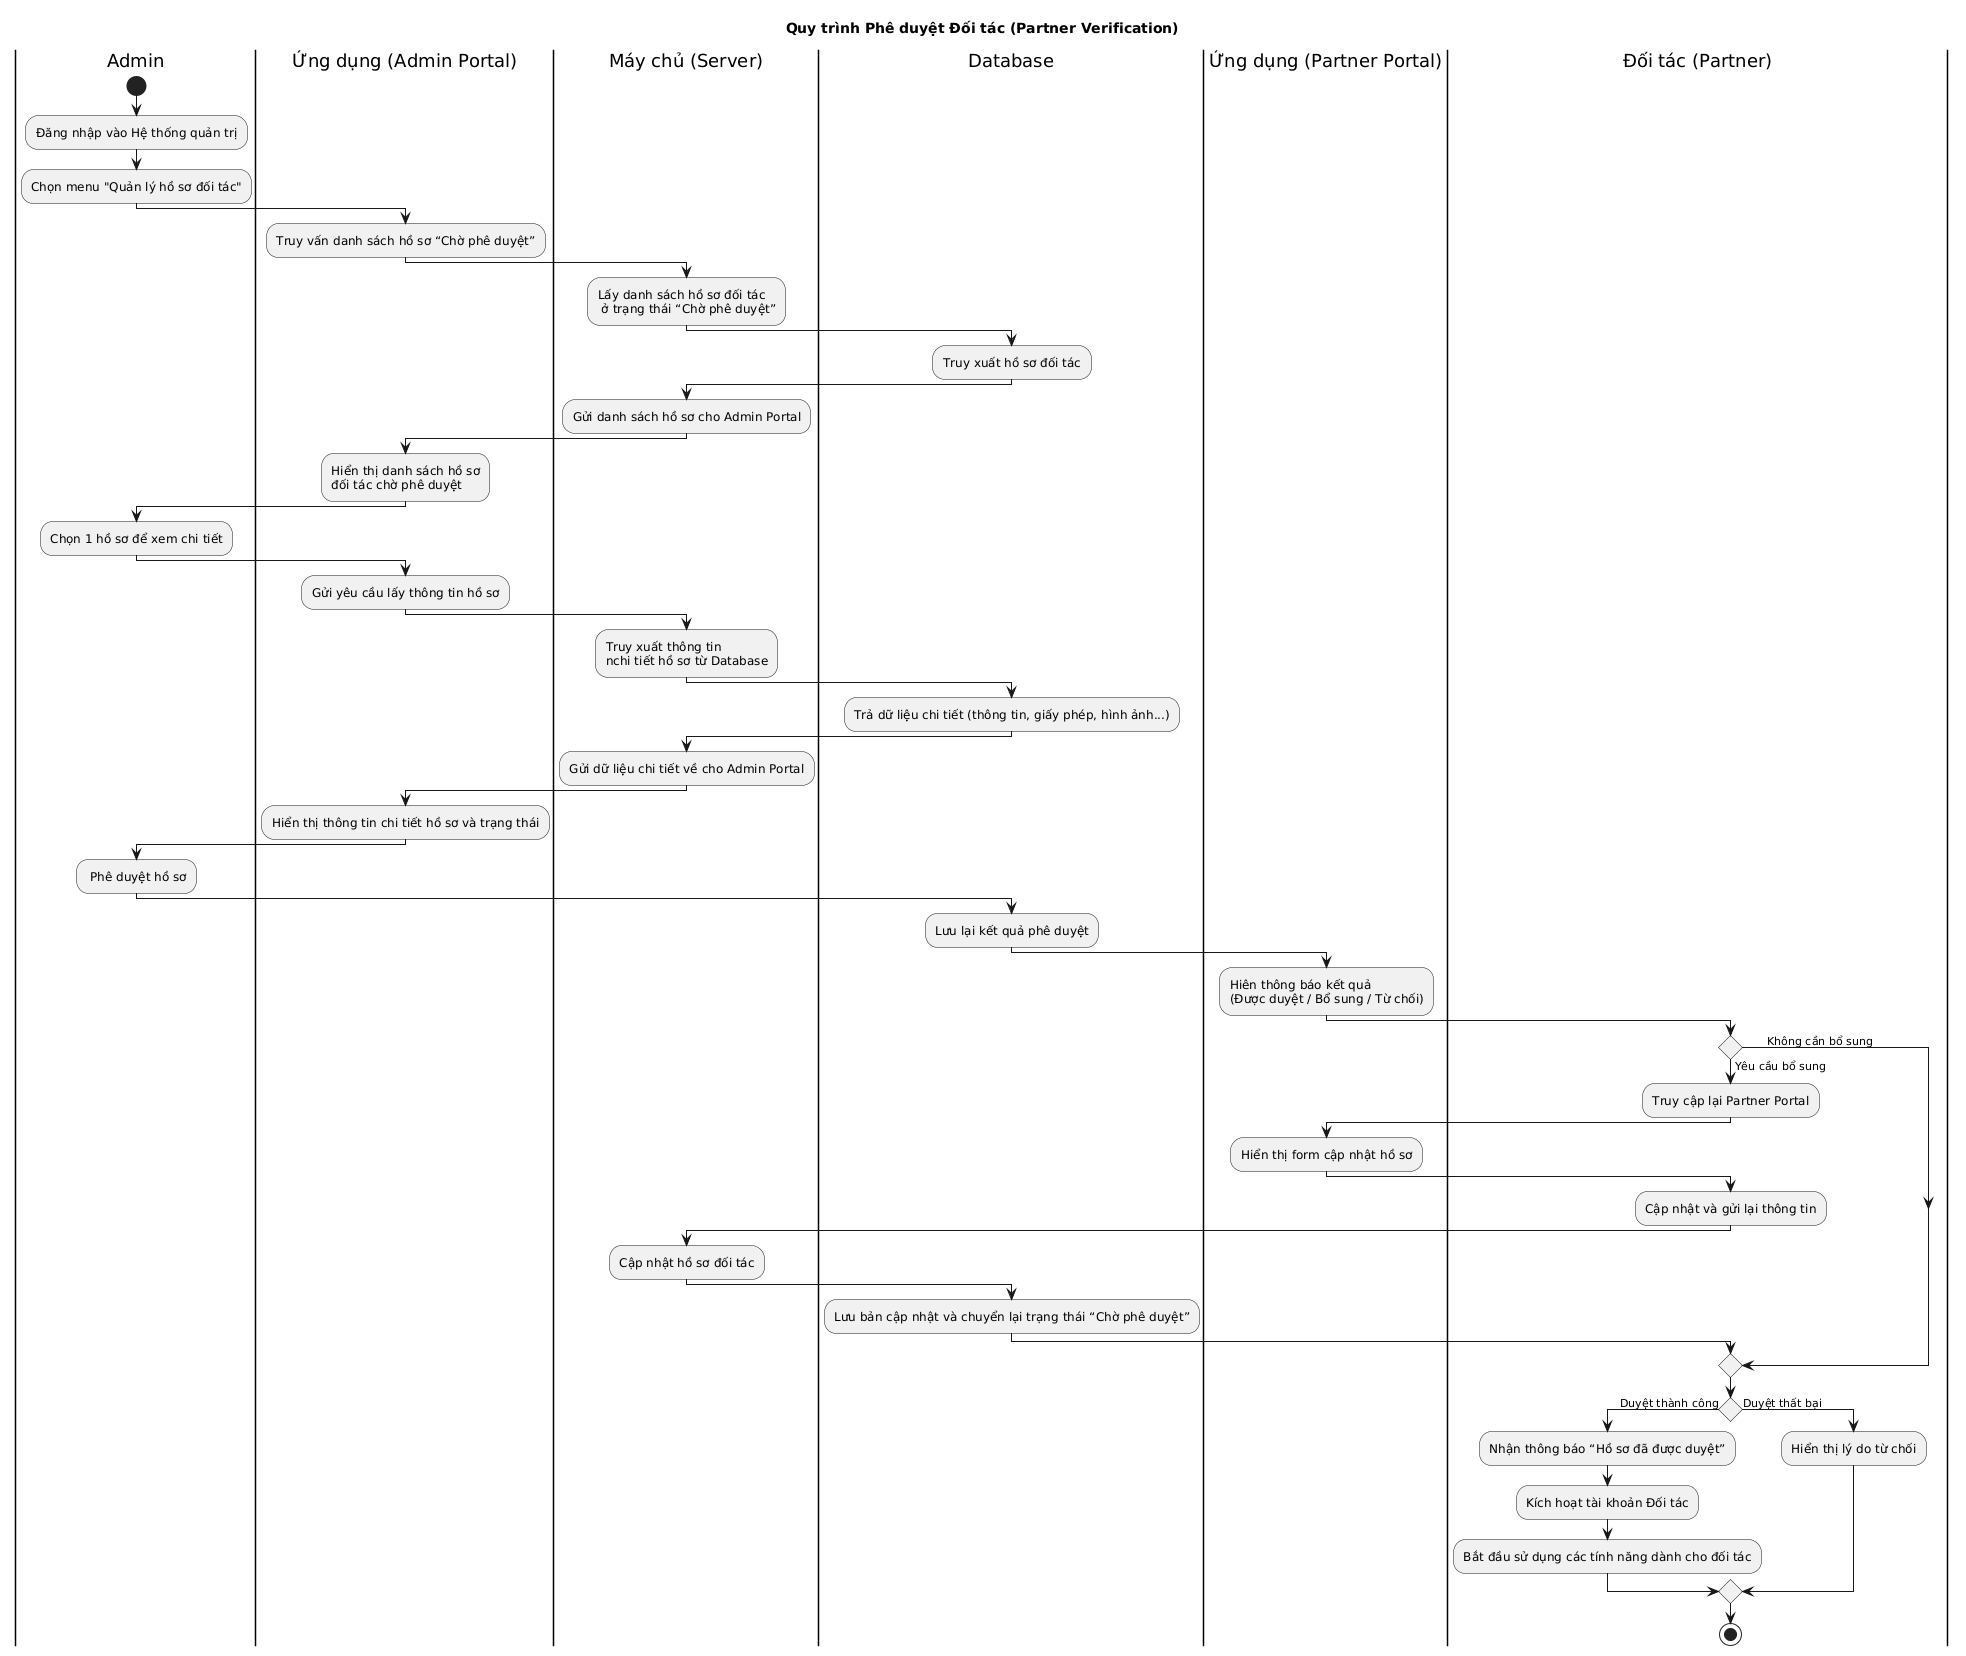
\includegraphics[width=0.8\textwidth]{Images/Activity/4.5.5.png}
\vspace{10pt}
    
    % Thêm chú thích cho hình ảnh
    \caption{Sơ đồ hoạt động Quy trình Phê duyệt Đối tác}

    % Đặt nhãn để tham chiếu chéo (cross-reference)
    \label{fig:activity_partner_verification}
\end{figure}
\subsection{Chu trình Tự động Huấn luyện Mô hình AI}
Sơ đồ này mô tả quy trình tự động thu thập và xử lý dữ liệu để huấn luyện mô hình AI. Dữ liệu hành vi của người dùng (như đặt lịch, tìm kiếm, đánh giá...) được ghi nhận bởi hệ thống backend và lưu trữ trong kho dữ liệu. Đến các chu kỳ huấn luyện định kỳ, hệ thống AI Pipeline sẽ truy xuất, làm sạch, trích xuất đặc trưng và tái huấn luyện mô hình nhằm cải thiện khả năng gợi ý, dự đoán hành vi và phân nhóm người dùng.

\begin{figure}[H]
    % Căn giữa hình ảnh
    \centering
    % Sử dụng width=1\textwidth để hình ảnh vừa với chiều rộng trang
    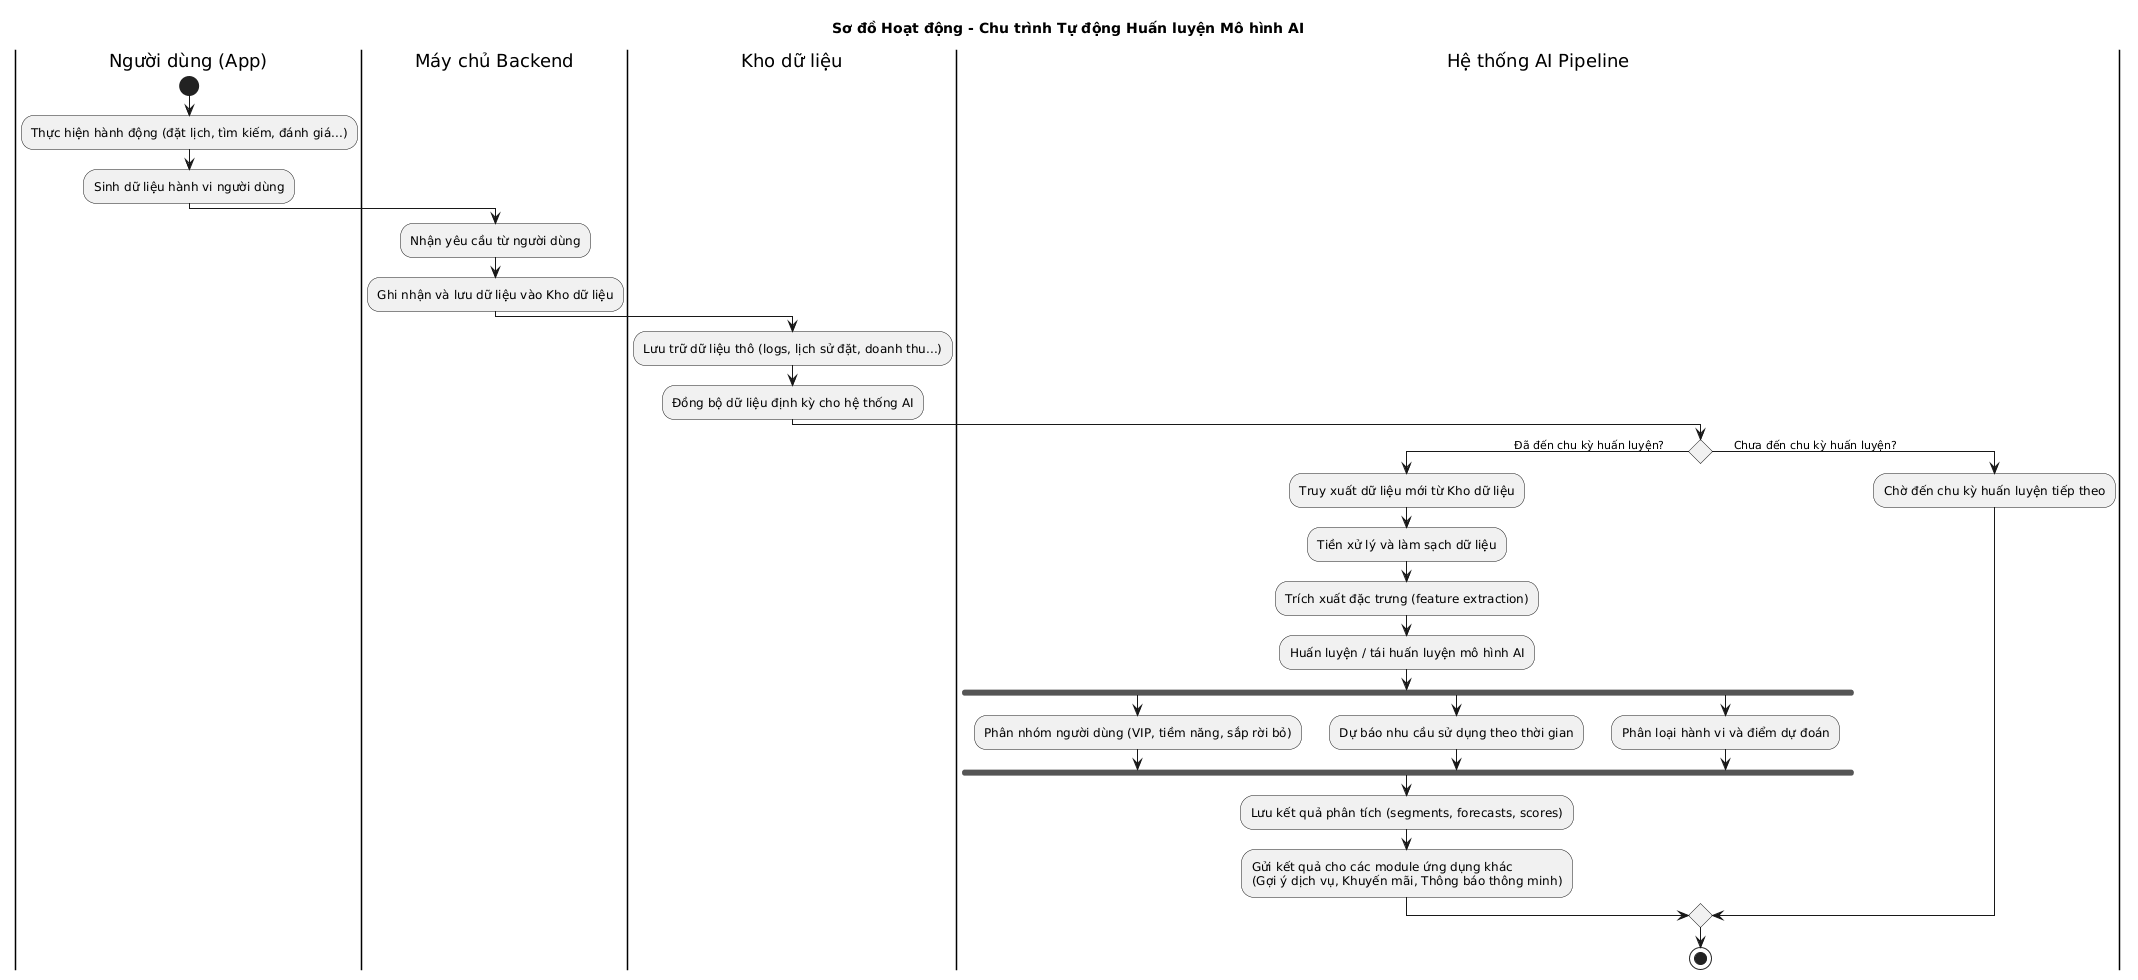
\includegraphics[width=0.8\textwidth]{Images/Activity/4.5.6.png}
    \vspace{10pt}

    % Thêm chú thích cho hình ảnh
    \caption{Sơ đồ hoạt động Chu trình Tự động Huấn luyện Mô hình AI}

    % Đặt nhãn để tham chiếu chéo (cross-reference)
    \label{fig:activity_ai_training_cycle}
\end{figure}


\subsection{Quản lý Lịch hẹn (Góc nhìn Đối tác / Dashboard)}
Sơ đồ này mô tả luồng hoạt động từ góc nhìn của Đối tác hoặc Nhân viên khi xử lý lịch hẹn qua Dashboard. Sau khi đăng nhập, họ nhận thông báo lịch hẹn mới, xem chi tiết thông tin và đưa ra quyết định xác nhận hoặc từ chối. Hệ thống gửi thông báo tương ứng đến người dùng, đồng thời sau khi hoàn tất dịch vụ, Đối tác đánh dấu hoàn tất để kích hoạt quy trình gửi yêu cầu đánh giá dịch vụ.

\begin{figure}[H]
    % Căn giữa hình ảnh
    \centering
    % Sử dụng width=1\textwidth để hình ảnh vừa với chiều rộng trang
    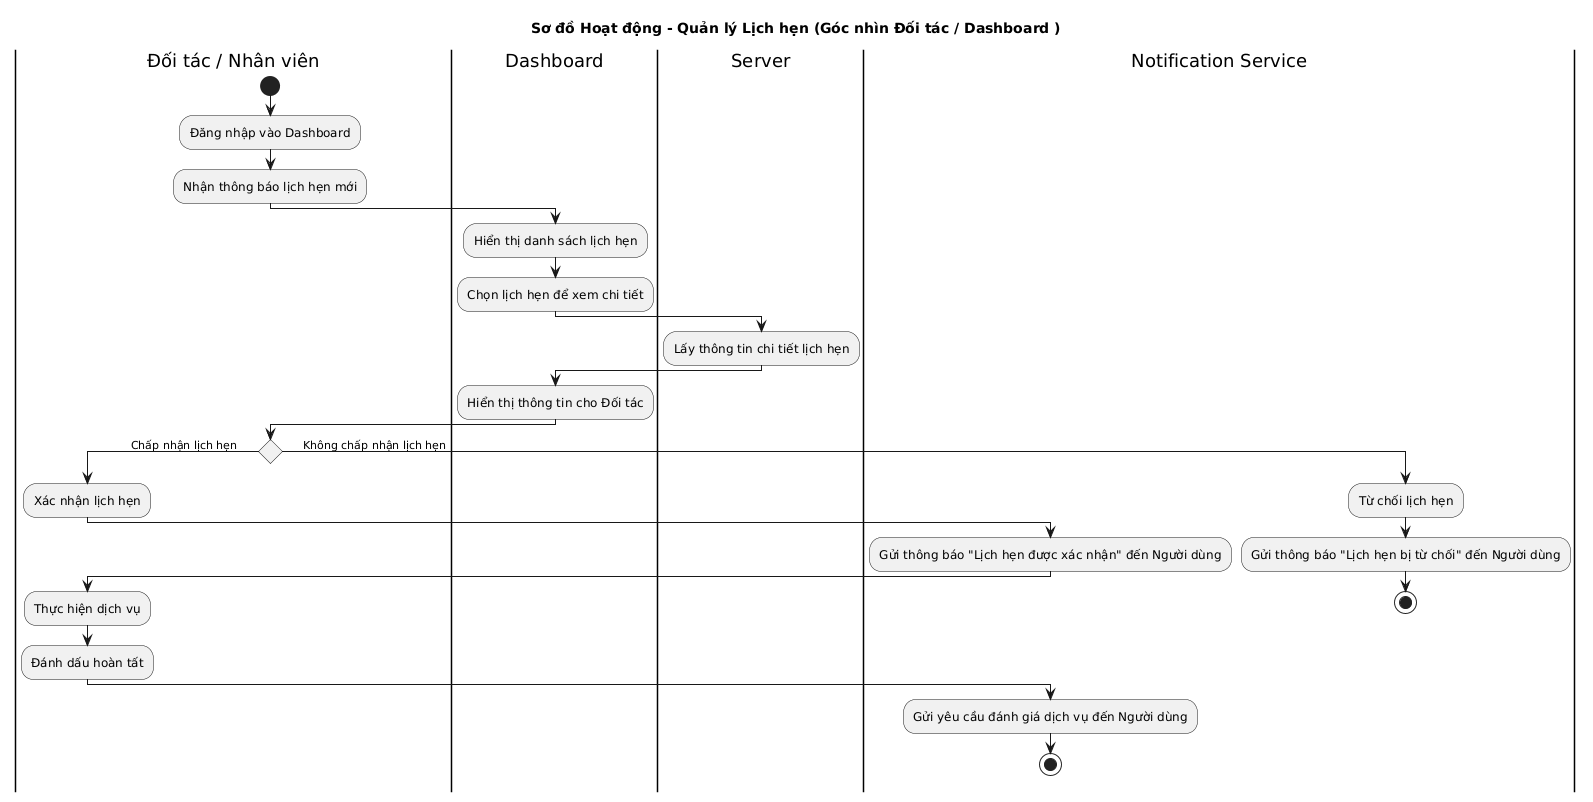
\includegraphics[width=0.8\textwidth]{Images/Activity/4.5.7.png}
    \vspace{10pt}

    % Thêm chú thích cho hình ảnh
    \caption{Sơ đồ hoạt động Quản lý Lịch hẹn (Góc nhìn Đối tác / Dashboard)}

    % Đặt nhãn để tham chiếu chéo (cross-reference)
    \label{fig:activity_partner_booking}
\end{figure}


\subsection{Quản lý Nhân viên \& Phân quyền}
Sơ đồ này mô tả quy trình quản lý nhân sự trong hệ thống dành cho Quản trị viên. Sau khi đăng nhập và truy cập trang quản lý nhân viên, Quản trị viên có thể thực hiện các hành động như thêm mới, cập nhật thông tin, phân quyền vai trò hoặc vô hiệu hóa tài khoản. Hệ thống xử lý yêu cầu tương ứng, cập nhật cơ sở dữ liệu và hiển thị kết quả trực tiếp trên Dashboard quản trị.

\begin{figure}[H]
    % Căn giữa hình ảnh
    \centering
    % Sử dụng width=1\textwidth để hình ảnh vừa với chiều rộng trang
    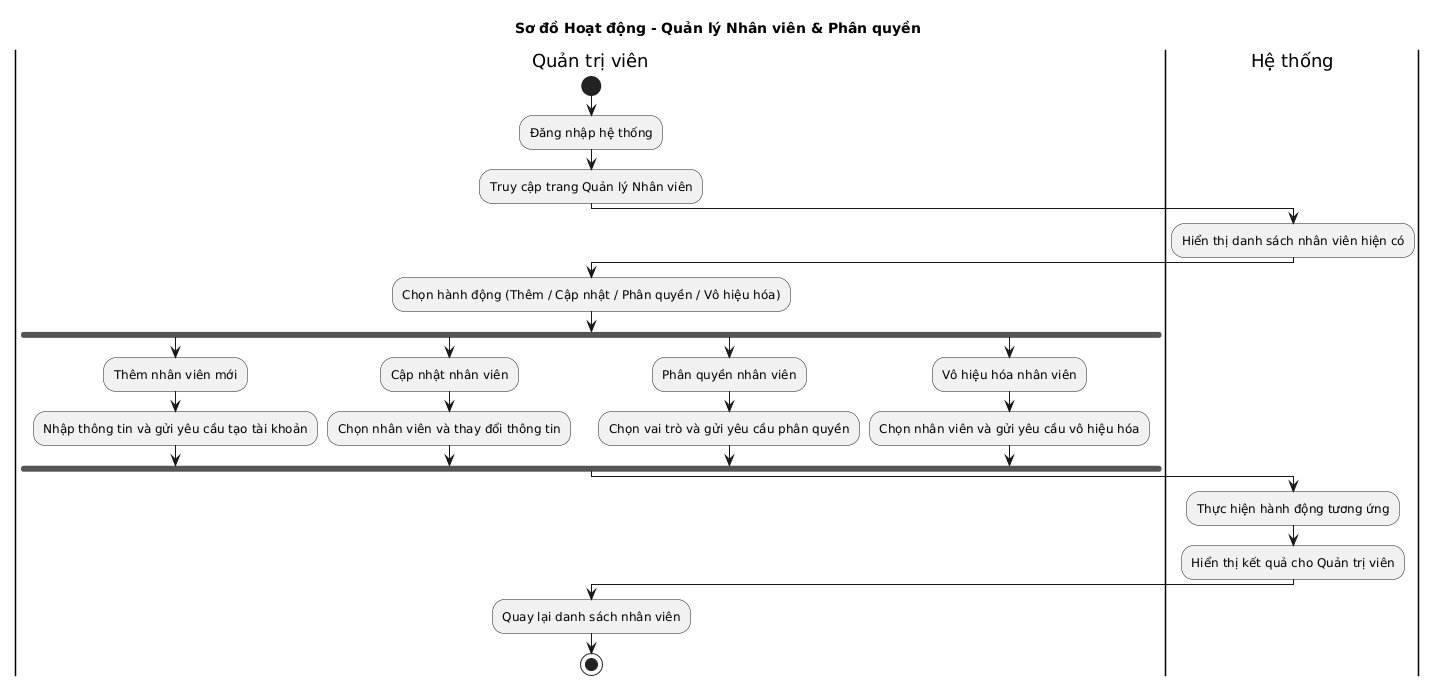
\includegraphics[width=0.8\textwidth]{Images/Activity/4.5.8.png}
    \vspace{10pt}

    % Thêm chú thích cho hình ảnh
    \caption{Sơ đồ hoạt động Quản lý Nhân viên \& Phân quyền}

    % Đặt nhãn để tham chiếu chéo (cross-reference)
    \label{fig:activity_staff_management}
\end{figure}

\section{Lược đồ Lớp (Class Diagram)}
\subsection{Mô tả}
Đây là một lược đồ lớp chi tiết, đóng vai trò là bản thiết kế cho cấu trúc của hệ thống. Mục đích chính của nó là định nghĩa các lớp đối tượng, thuộc tính, phương thức và mối quan hệ logic giữa chúng. Lược đồ được phân chia rõ ràng thành các domain chính: Ứng dụng Người dùng (User App), Cổng Đối tác (Partner Portal), Bảng điều khiển Quản trị viên (Admin Dashboard), và một Lõi (Core) dùng chung.
\subsection{Lược đồ tổng quan}
\begin{figure}[H]
    % Căn giữa hình ảnh
    \centering
    
\includegraphics[width=1\textwidth]{Images/ClassDiagram/class_diagram.png}
    \vspace{10pt}
    
    % Thêm chú thích cho hình ảnh
    \caption{Class Diagram của hệ thống}
    
    % Đặt nhãn để tham chiếu chéo (cross-reference)
    \label{fig:class_diagram}
\end{figure}
\subsection{Các thành phần chính và mối quan hệ}
 Hệ thống xoay quanh ba tác nhân chính: User (khách hàng cuối), Partner (doanh nghiệp cung cấp dịch vụ), và Admin (người quản trị hệ thống).
\subsubsection{Phân hệ 1: Quản lý Người dùng \& Bảo mật (Identity \& Access Management)}

Phân hệ này chịu trách nhiệm xác thực (Authentication) và phân quyền (Authorization) cho toàn bộ hệ thống. Nó đảm bảo tính bảo mật và quản lý phiên làm việc.

\begin{figure}[H]
    \centering
    % Thay 'module_user.png' bằng tên file ảnh bạn đã export từ Mermaid/Draw.io
    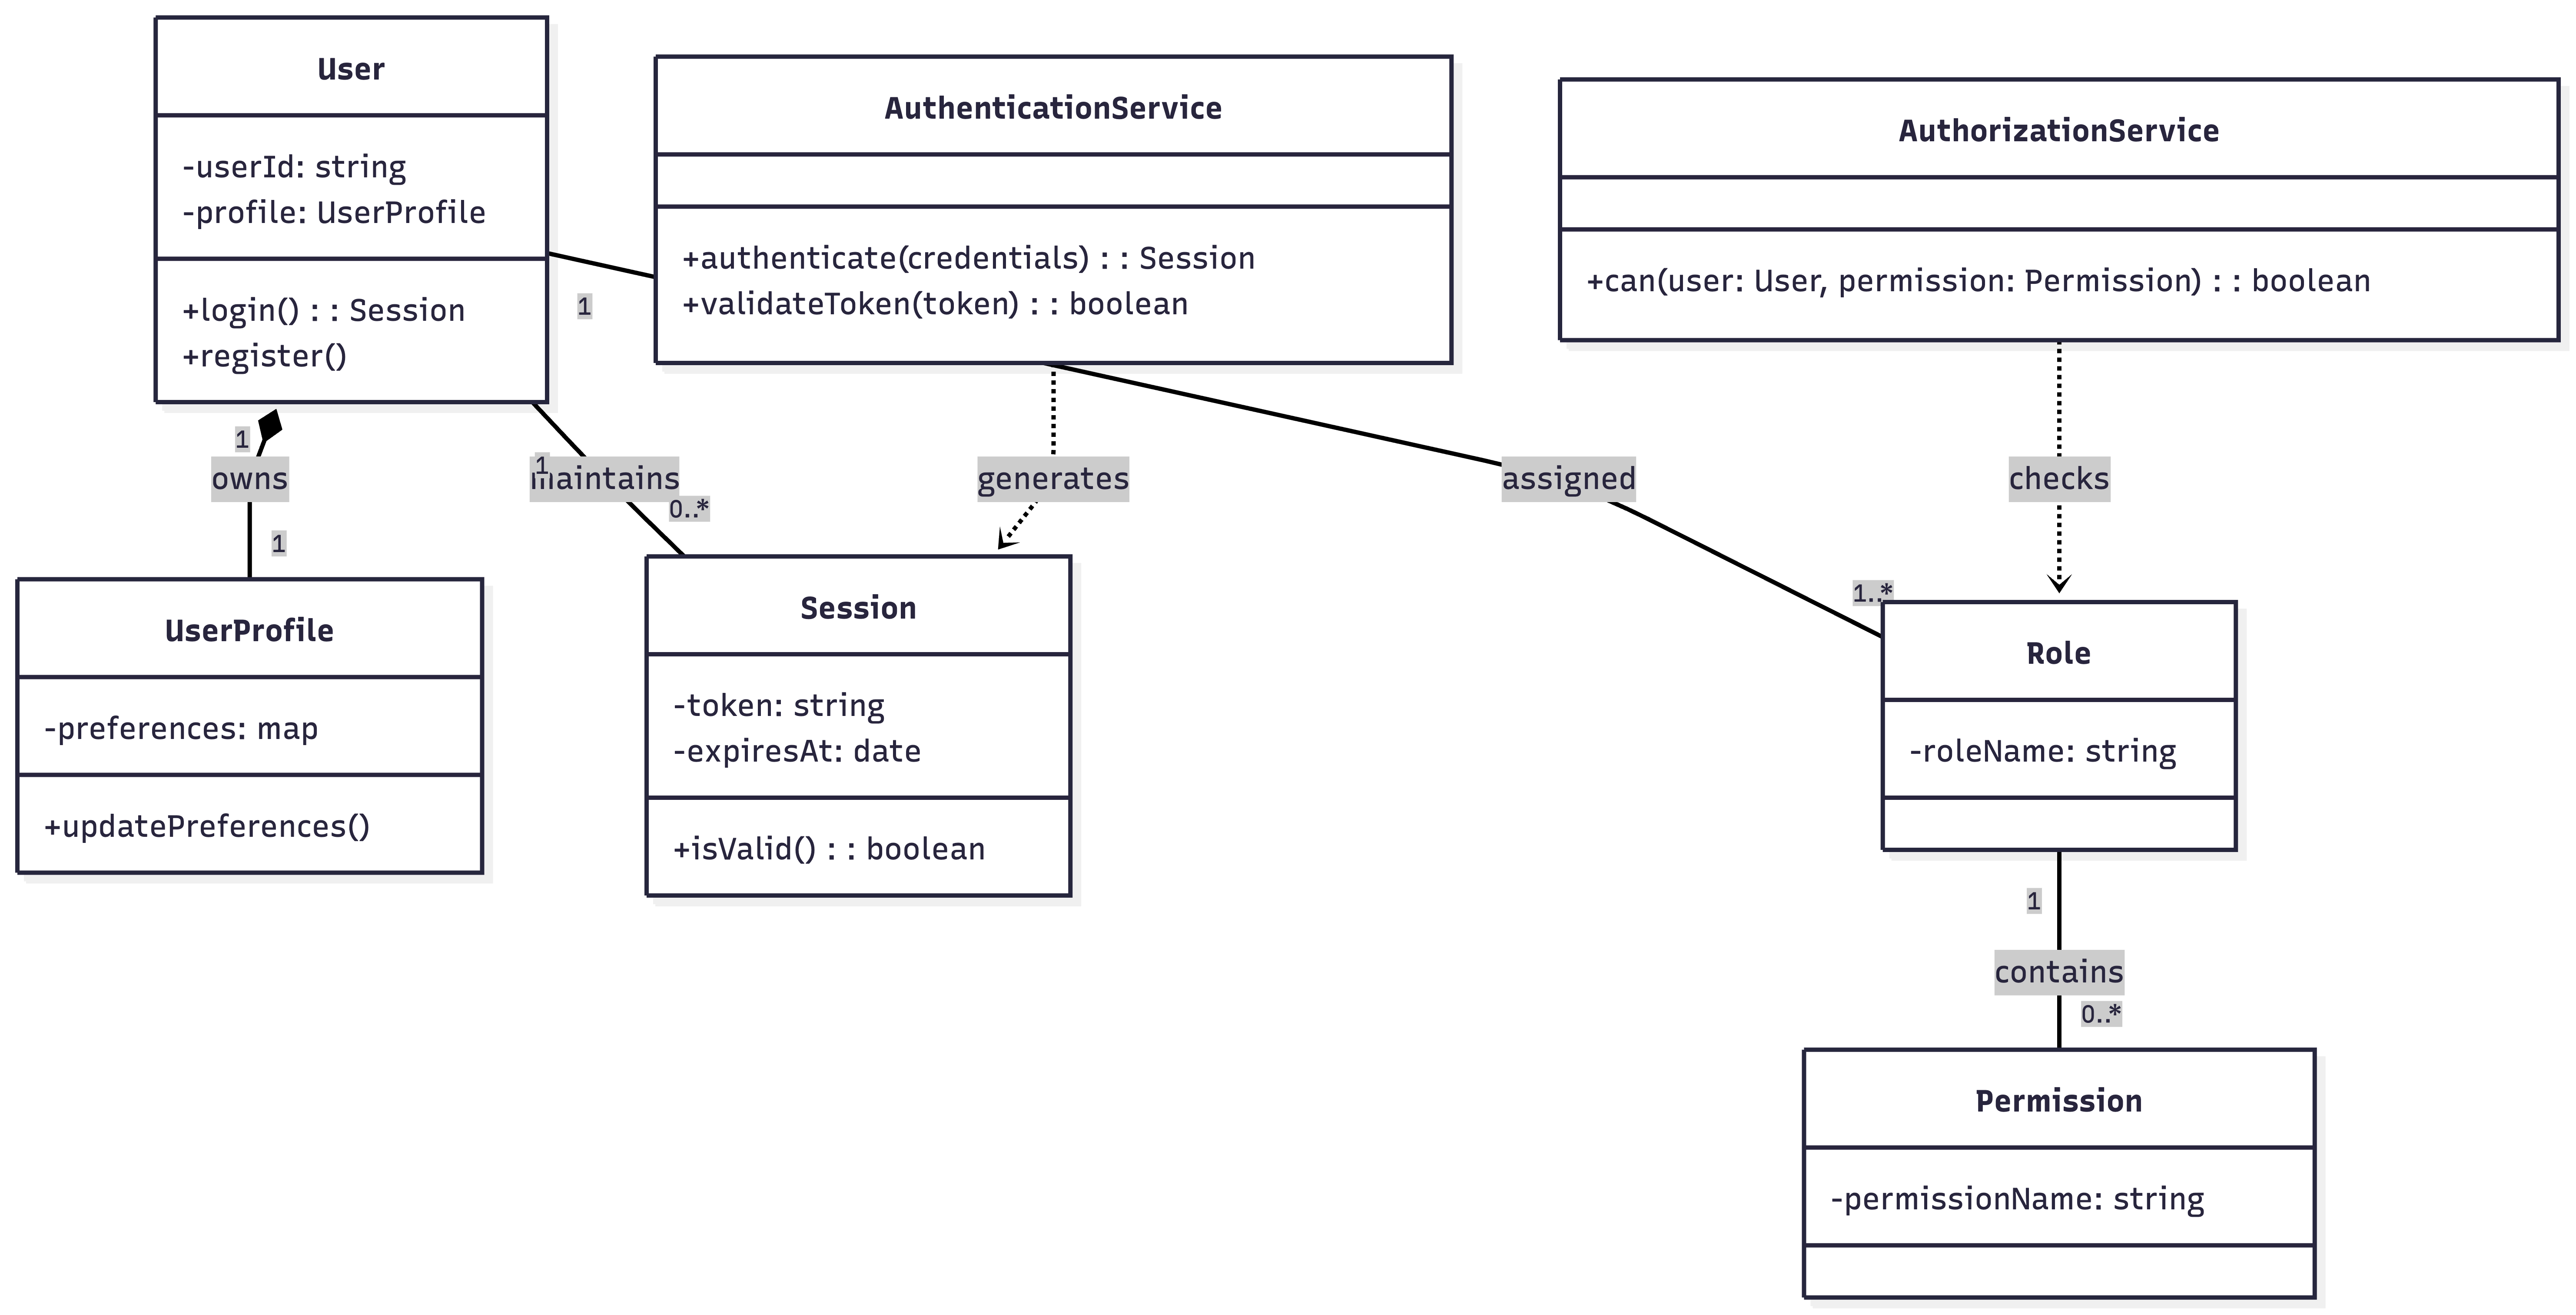
\includegraphics[width=0.8\textwidth]{Images/ClassDiagram/module_user.png}
    \vspace{10pt}
    
    \caption{Sơ đồ lớp phân hệ Quản lý Người dùng}
    \label{fig:module_user}
\end{figure}

\subsubsection*{Giải thích chi tiết:}
\begin{itemize}
    \item \textbf{User \& UserProfile:} Áp dụng nguyên lý \textit{Separation of Concerns}. Lớp \texttt{User} chỉ chứa thông tin định danh (Account), trong khi \texttt{UserProfile} chứa thông tin cá nhân và sở thích. Quan hệ Composition thể hiện \texttt{UserProfile} không thể tồn tại nếu thiếu \texttt{User}.
    \item \textbf{RBAC (Role-Based Access Control):} Hệ thống sử dụng mô hình RBAC thông qua các lớp \texttt{Role} và \texttt{Permission}. Một User có nhiều Role (VD: Partner, Admin), và một Role bao gồm nhiều Permission.
    \item \textbf{Services:}
    \begin{itemize}
        \item \texttt{AuthenticationService}: Chịu trách nhiệm cấp phát Session/Token (như JWT).
        \item \texttt{AuthorizationService}: Kiểm tra xem User có quyền thực hiện hành động cụ thể không dựa trên Role của họ.
    \end{itemize}
\end{itemize}

% --- PHÂN HỆ 2 ---
\subsubsection{Phân hệ 2: Nghiệp vụ cốt lõi - Đặt lịch \& Thanh toán (Core Business)}

Đây là trái tim của hệ thống, xử lý luồng đi từ lúc người dùng đặt dịch vụ đến khi thanh toán hoàn tất. Phân hệ này áp dụng nhiều mẫu thiết kế (Design Patterns).

\begin{figure}[H]
    \centering
    % Thay 'module_booking.png' bằng tên file ảnh của bạn
    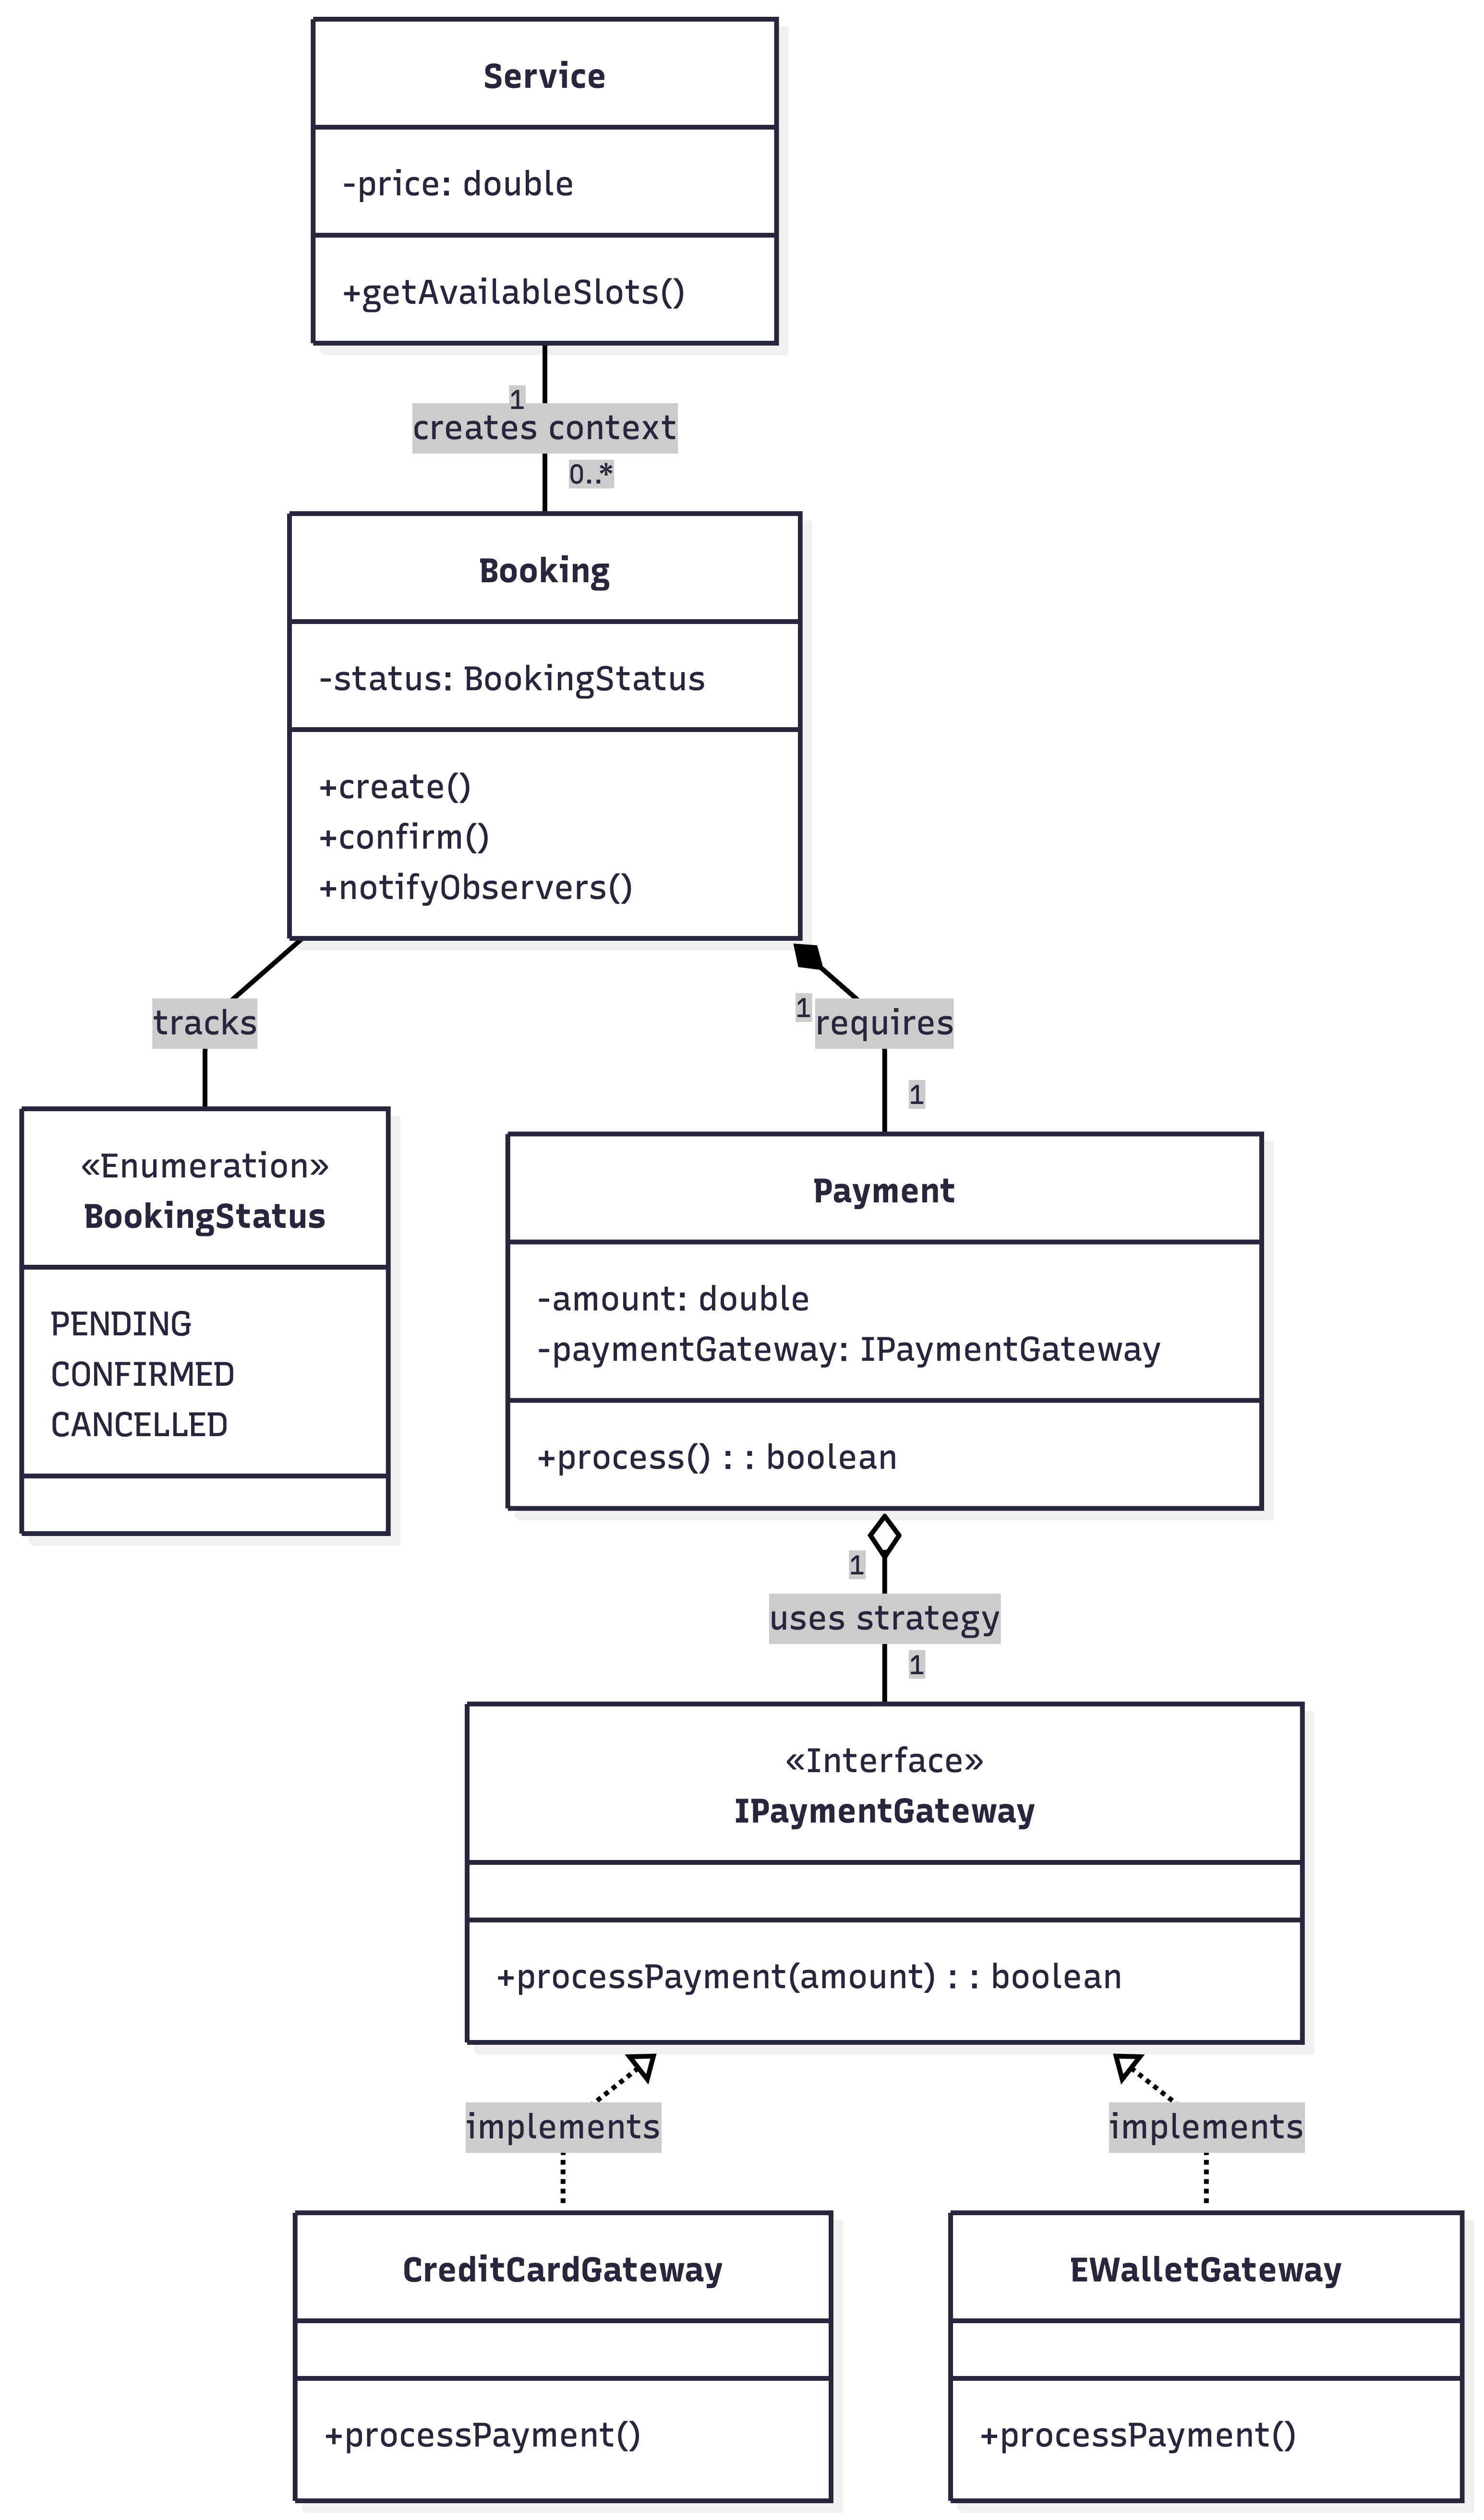
\includegraphics[width=0.8\textwidth]{Images/ClassDiagram/module_booking.png}
    \vspace{10pt}
    
    \caption{Sơ đồ lớp phân hệ Đặt lịch \& Thanh toán}
    \label{fig:module_booking}
\end{figure}

\subsubsubsection*{Giải thích chi tiết:}
\begin{itemize}
    \item \textbf{Booking Lifecycle:} Lớp \texttt{Booking} quản lý trạng thái đơn hàng thông qua \texttt{BookingStatus} (Enumeration) để đảm bảo tính nhất quán của dữ liệu.
    \item \textbf{Strategy Pattern (Payment):}
    \begin{itemize}
        \item \texttt{IPaymentGateway} đóng vai trò là Interface chung.
        \item \texttt{CreditCardGateway} và \texttt{EWalletGateway} là các thuật toán xử lý thanh toán cụ thể.
        \item \textit{Lợi ích:} Giúp hệ thống tuân thủ nguyên lý \textit{Open/Closed (SOLID)}. Khi cần tích hợp cổng thanh toán mới, chỉ cần tạo lớp mới implement interface mà không cần sửa code cũ.
    \end{itemize}
    \item \textbf{Quan hệ:} Một Booking bắt buộc phải có một Payment (Composition), đảm bảo không có đơn hàng nào tồn tại mà không gắn liền với thông tin thanh toán.
\end{itemize}

% --- PHÂN HỆ 3 ---
\subsubsection{Phân hệ 3: Đối tác \& Vận hành dịch vụ (Partner Operations)}

Phân hệ này quản lý phía cung cấp dịch vụ (Supply side), bao gồm quản lý nhân viên, báo cáo tài chính và dịch vụ cung cấp.

\begin{figure}[H]
    \centering
    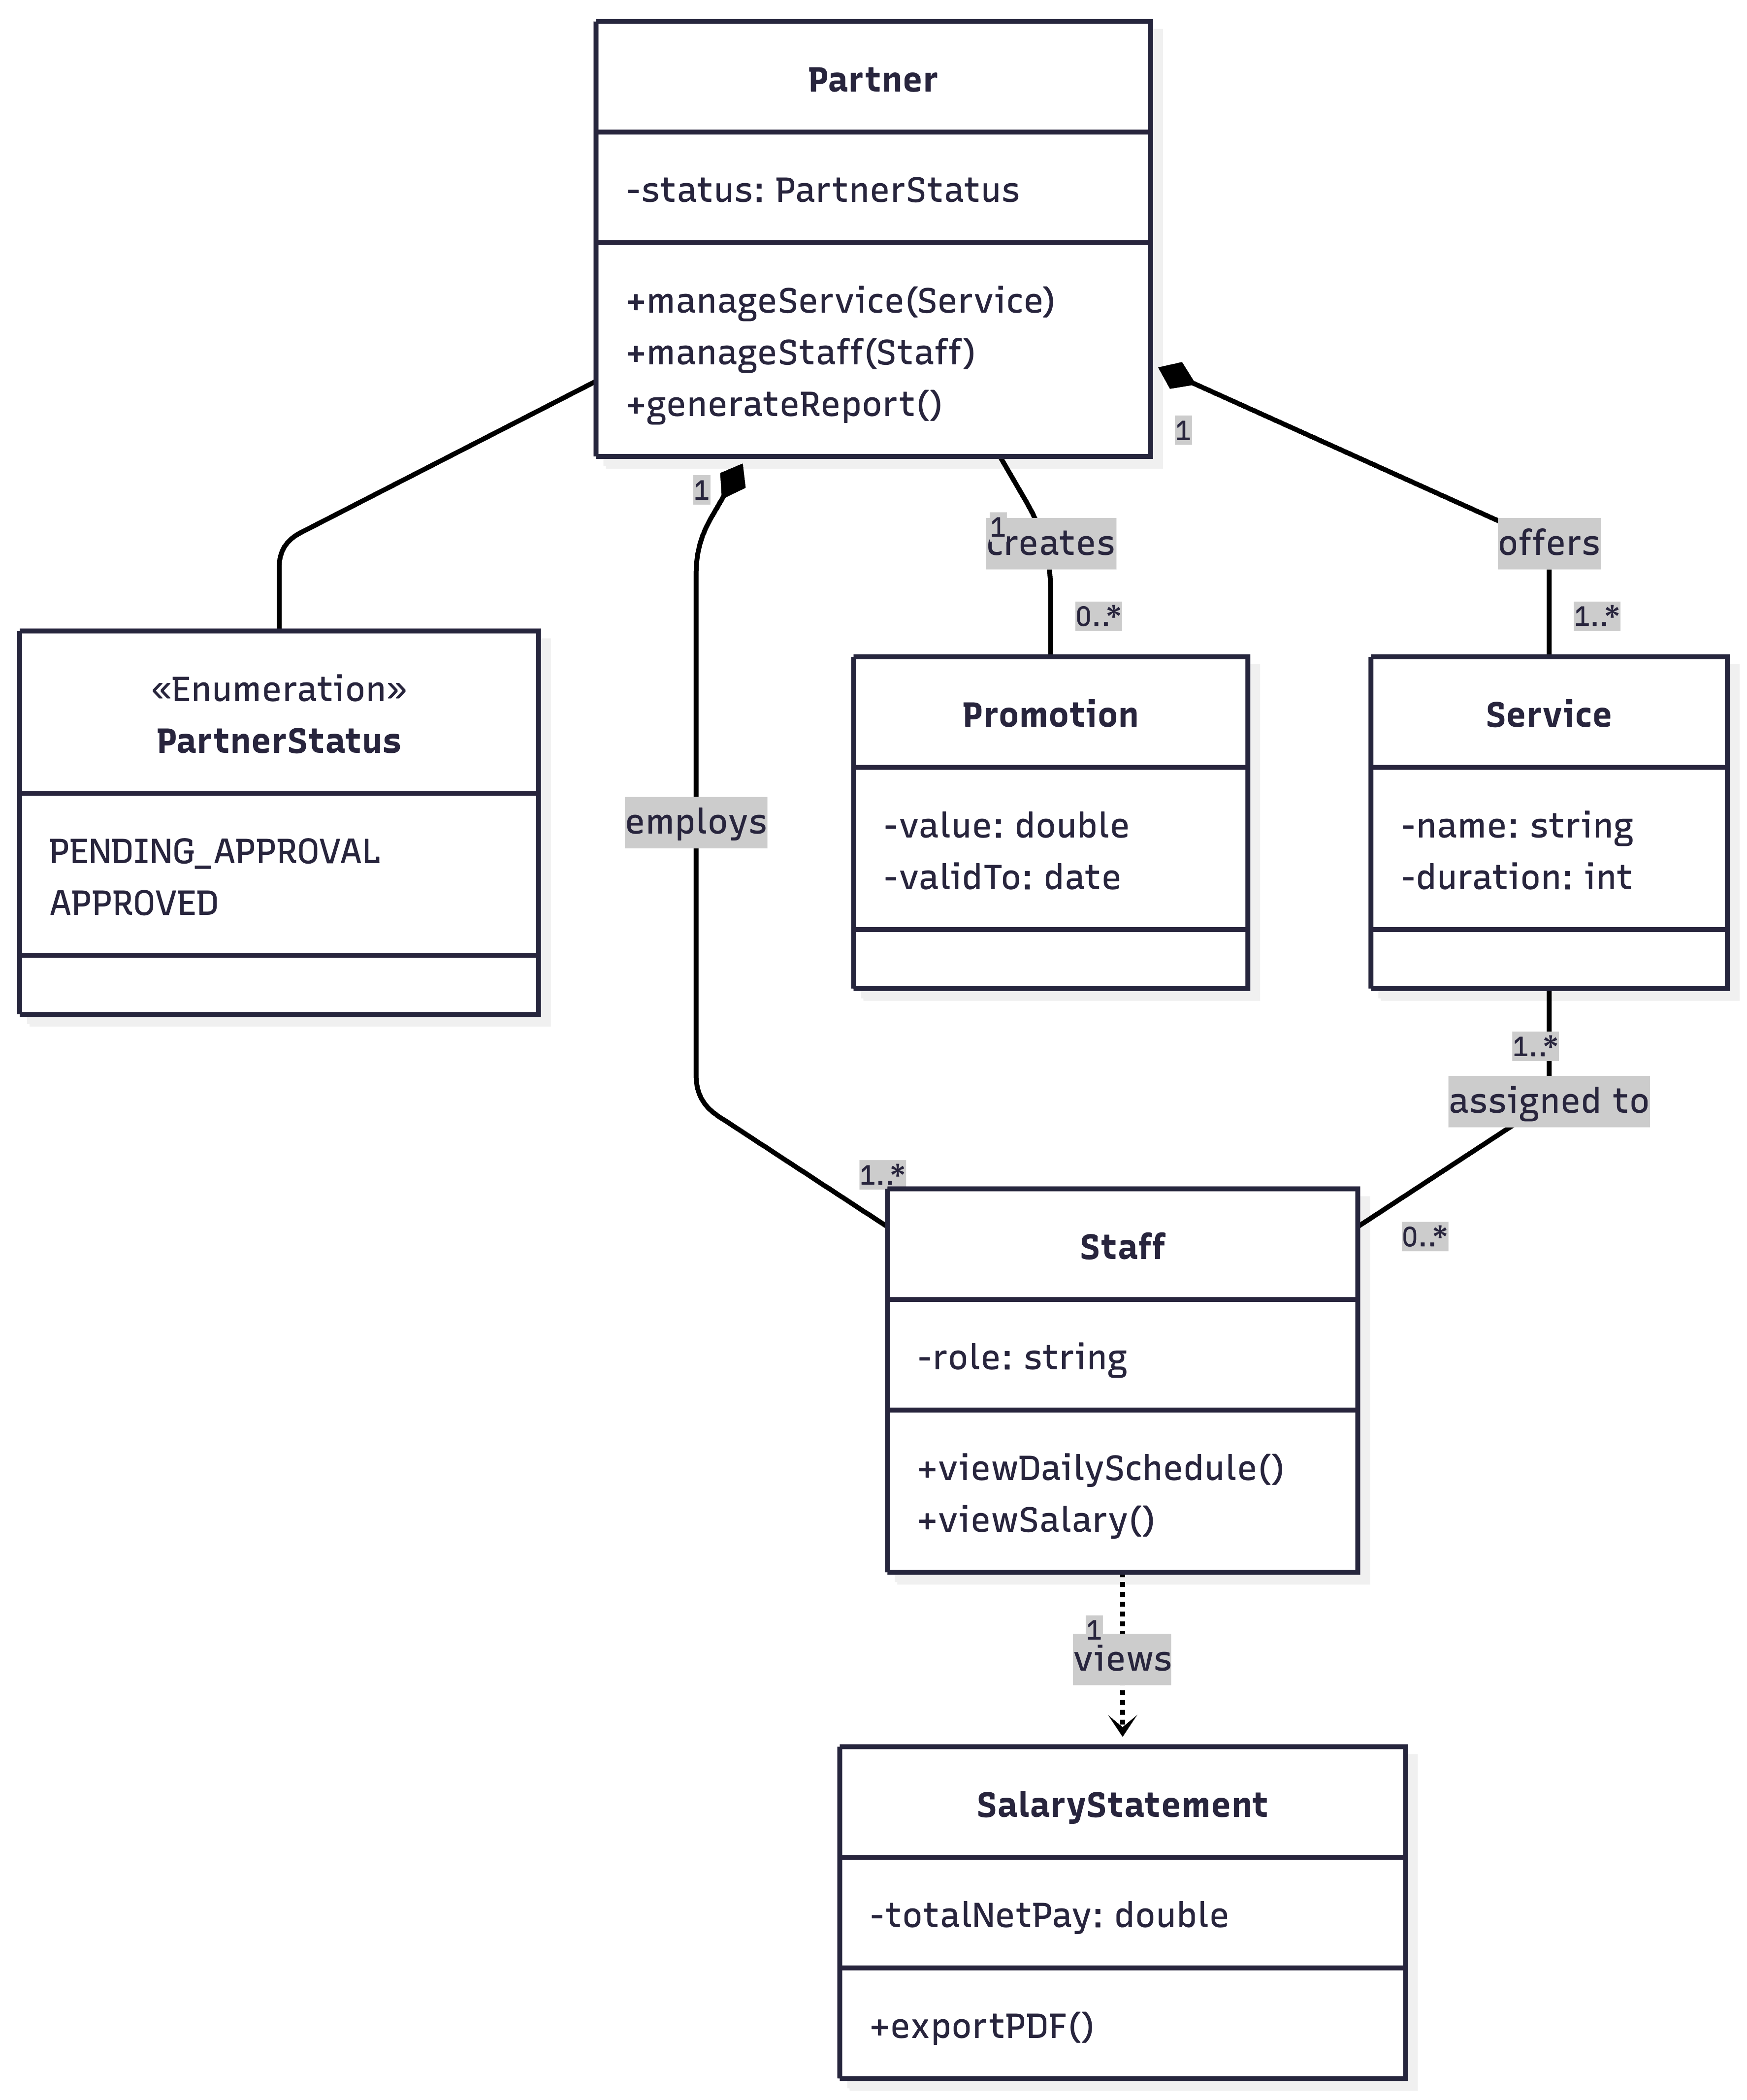
\includegraphics[width=0.8\textwidth]{Images/ClassDiagram/module_partner.png}
    \vspace{10pt}
    
    \caption{Sơ đồ lớp phân hệ Đối tác}
    \label{fig:module_partner}
\end{figure}

\subsubsubsection*{Giải thích chi tiết:}
\begin{itemize}
    \item \textbf{Mô hình Quản lý tập trung:} \texttt{Partner} là thực thể trung tâm (Root Aggregate). Nó sở hữu vòng đời của \texttt{Service} và \texttt{Staff}. Nếu Partner bị xóa, các dịch vụ và nhân viên liên quan cũng sẽ được xử lý tương ứng.
    \item \textbf{Staff \& Service:} Mối quan hệ N-N giúp linh hoạt trong việc xếp lịch (Scheduling).
    \item \textbf{Promotion:} Partner có quyền tự tạo các chương trình khuyến mãi, tách biệt với logic giá gốc của Service.
\end{itemize}

% --- PHÂN HỆ 4 ---
\subsubsection{Phân hệ 4: Thông báo \& Tương tác (Communication)}

Phân hệ này xử lý việc gửi tin tức đến người dùng và các tương tác hỗ trợ (Chatbot, Support Ticket).

\begin{figure}[H]
    \centering
    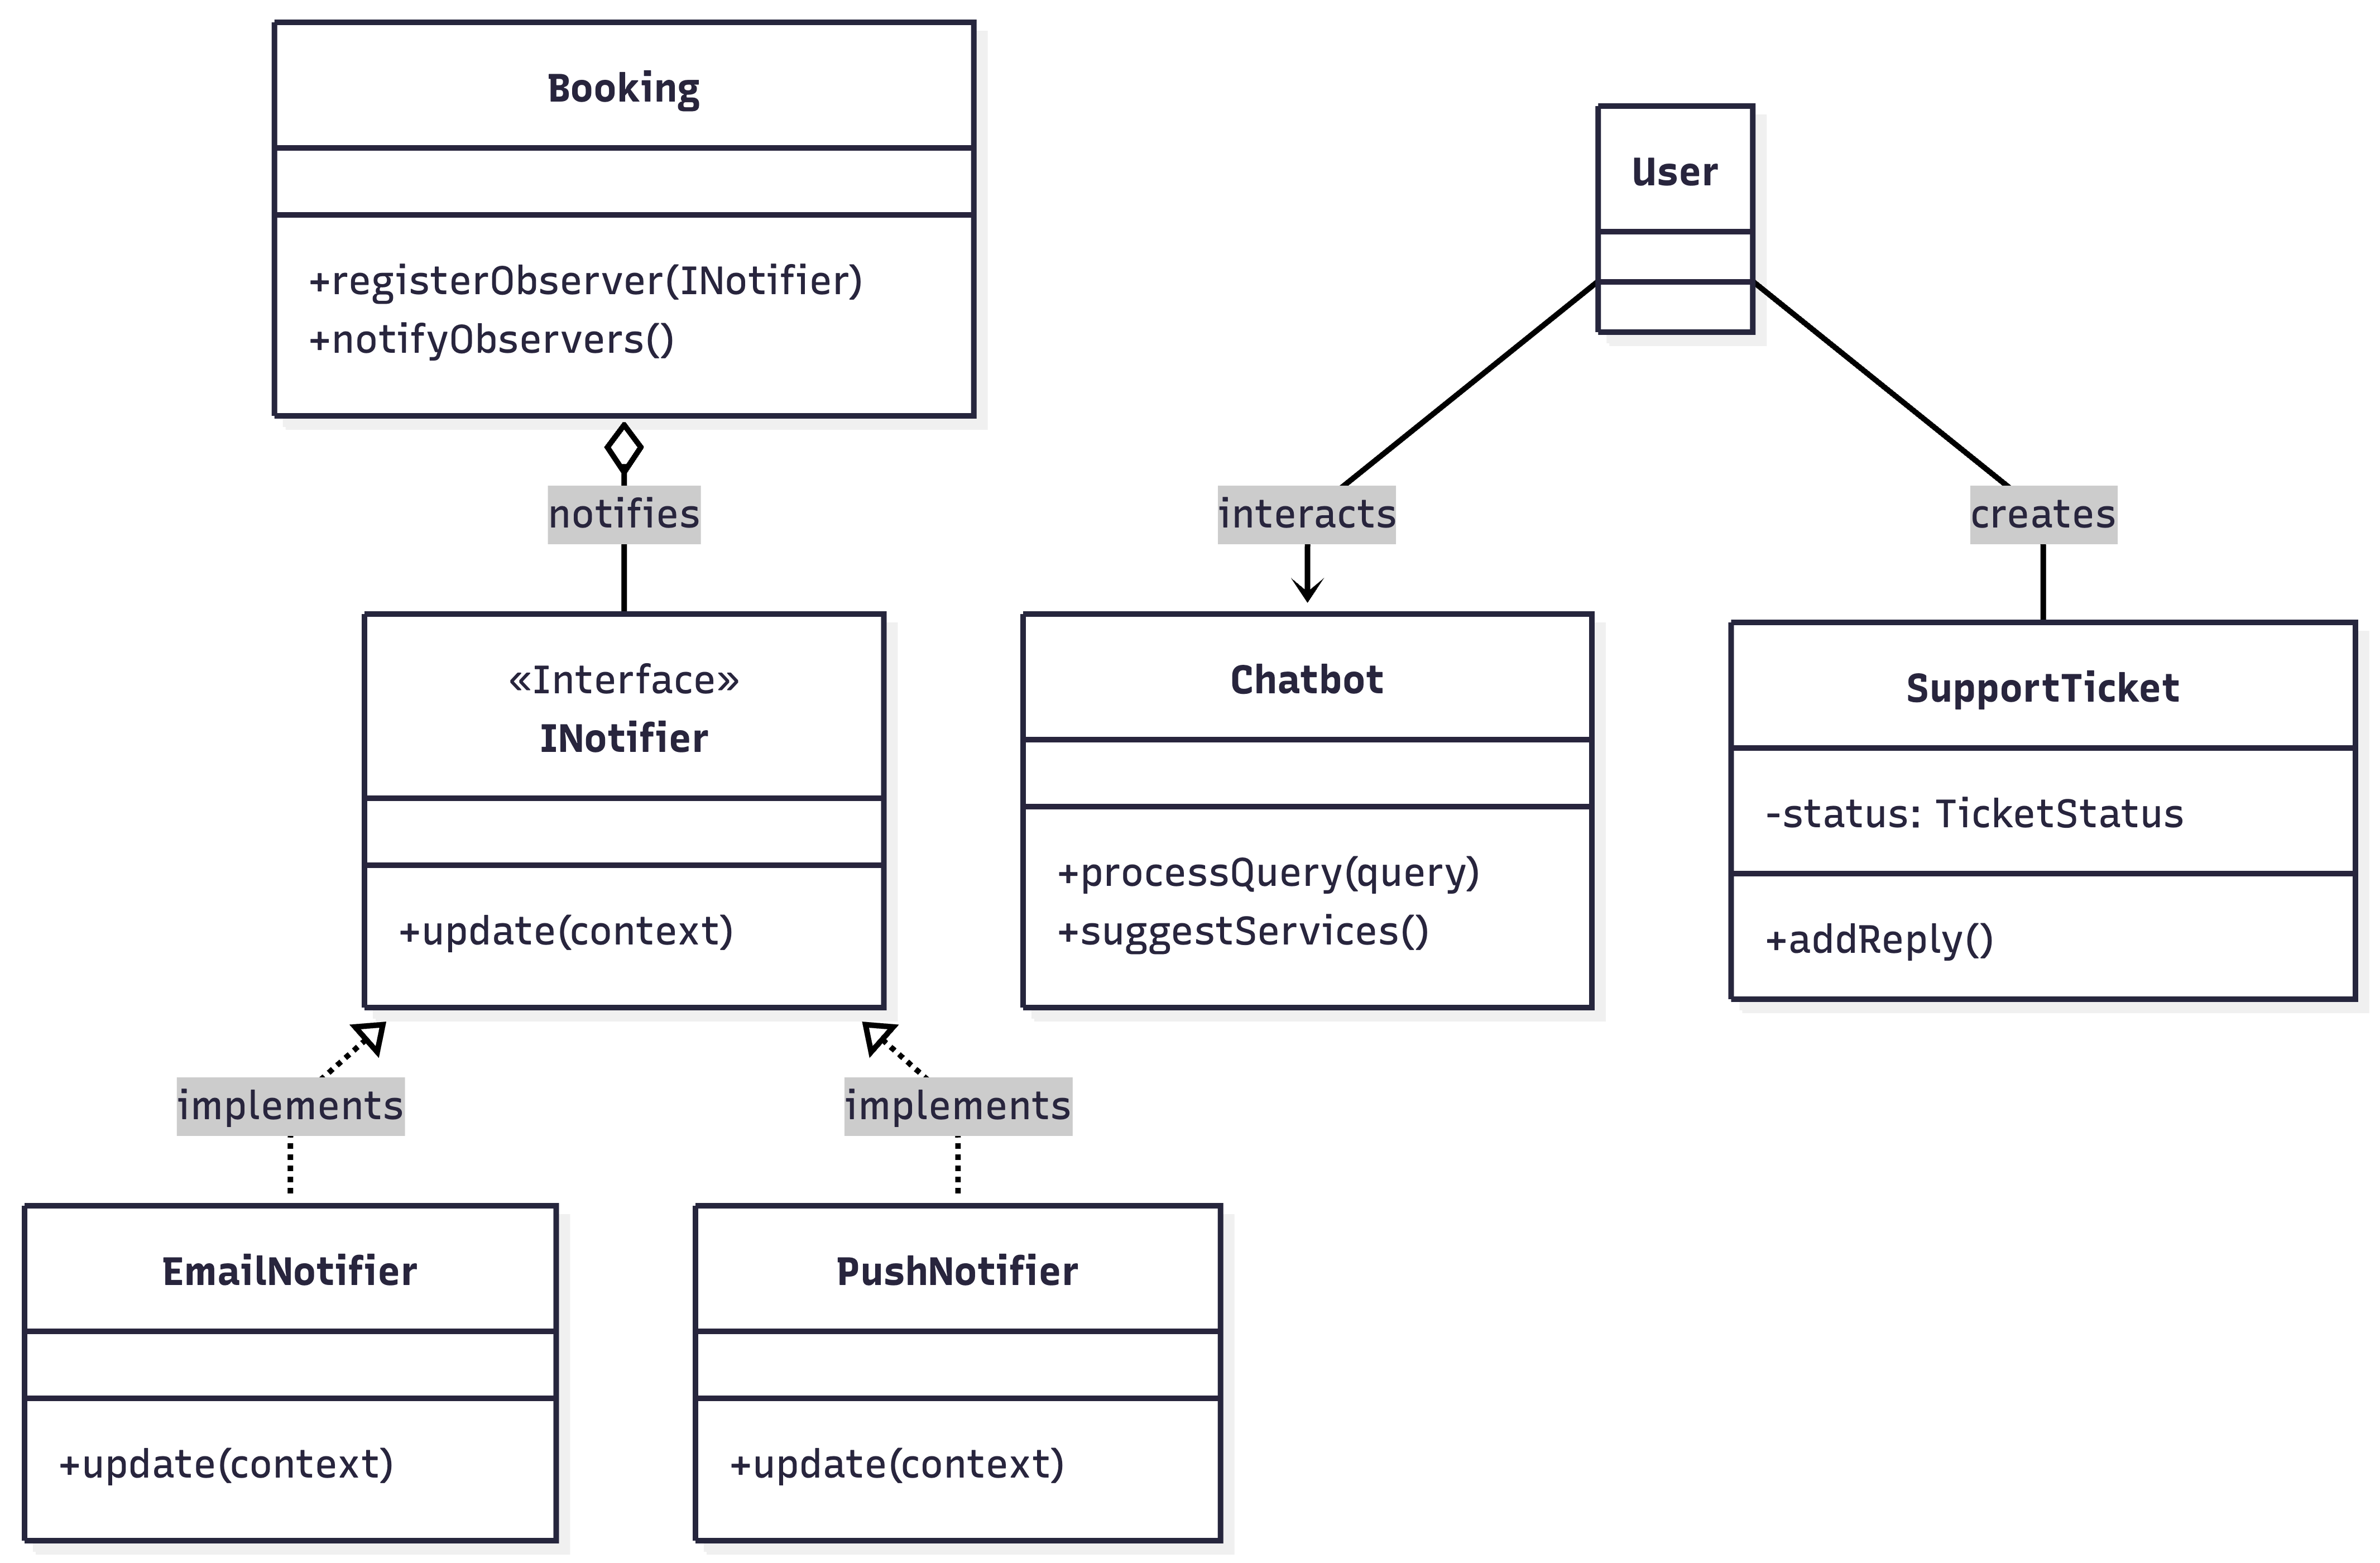
\includegraphics[width=0.8\textwidth]{Images/ClassDiagram/module_communication.png}
    \vspace{10pt}
    
    \caption{Sơ đồ lớp phân hệ Thông báo}
    \label{fig:module_comm}
\end{figure}

\subsubsubsection*{Giải thích chi tiết:}
\begin{itemize}
    \item \textbf{Observer Pattern:} Hệ thống áp dụng mẫu Observer cho việc thông báo.
    \begin{itemize}
        \item \texttt{Booking} đóng vai trò là \textit{Subject}.
        \item \texttt{EmailNotifier} và \texttt{PushNotifier} là các \textit{Observers}.
        \item Khi trạng thái Booking thay đổi, nó tự động gọi \texttt{notifyObservers()}, giúp tách rời logic xử lý đơn hàng khỏi logic gửi tin (Decoupling).
    \end{itemize}
    \item \textbf{Chatbot:} Được thiết kế để xử lý ngôn ngữ tự nhiên (NLP) và gợi ý dịch vụ. Class này thường áp dụng mẫu \textit{Singleton} để tiết kiệm tài nguyên kết nối AI.
\end{itemize}

% --- PHÂN HỆ 5 ---
\subsubsection{Phân hệ 5: Quản trị hệ thống (Administration)}

Phân hệ dành cho Admin để kiểm duyệt, quản lý rủi ro và theo dõi sức khỏe tài chính của nền tảng.

\begin{figure}[H]
    \centering
    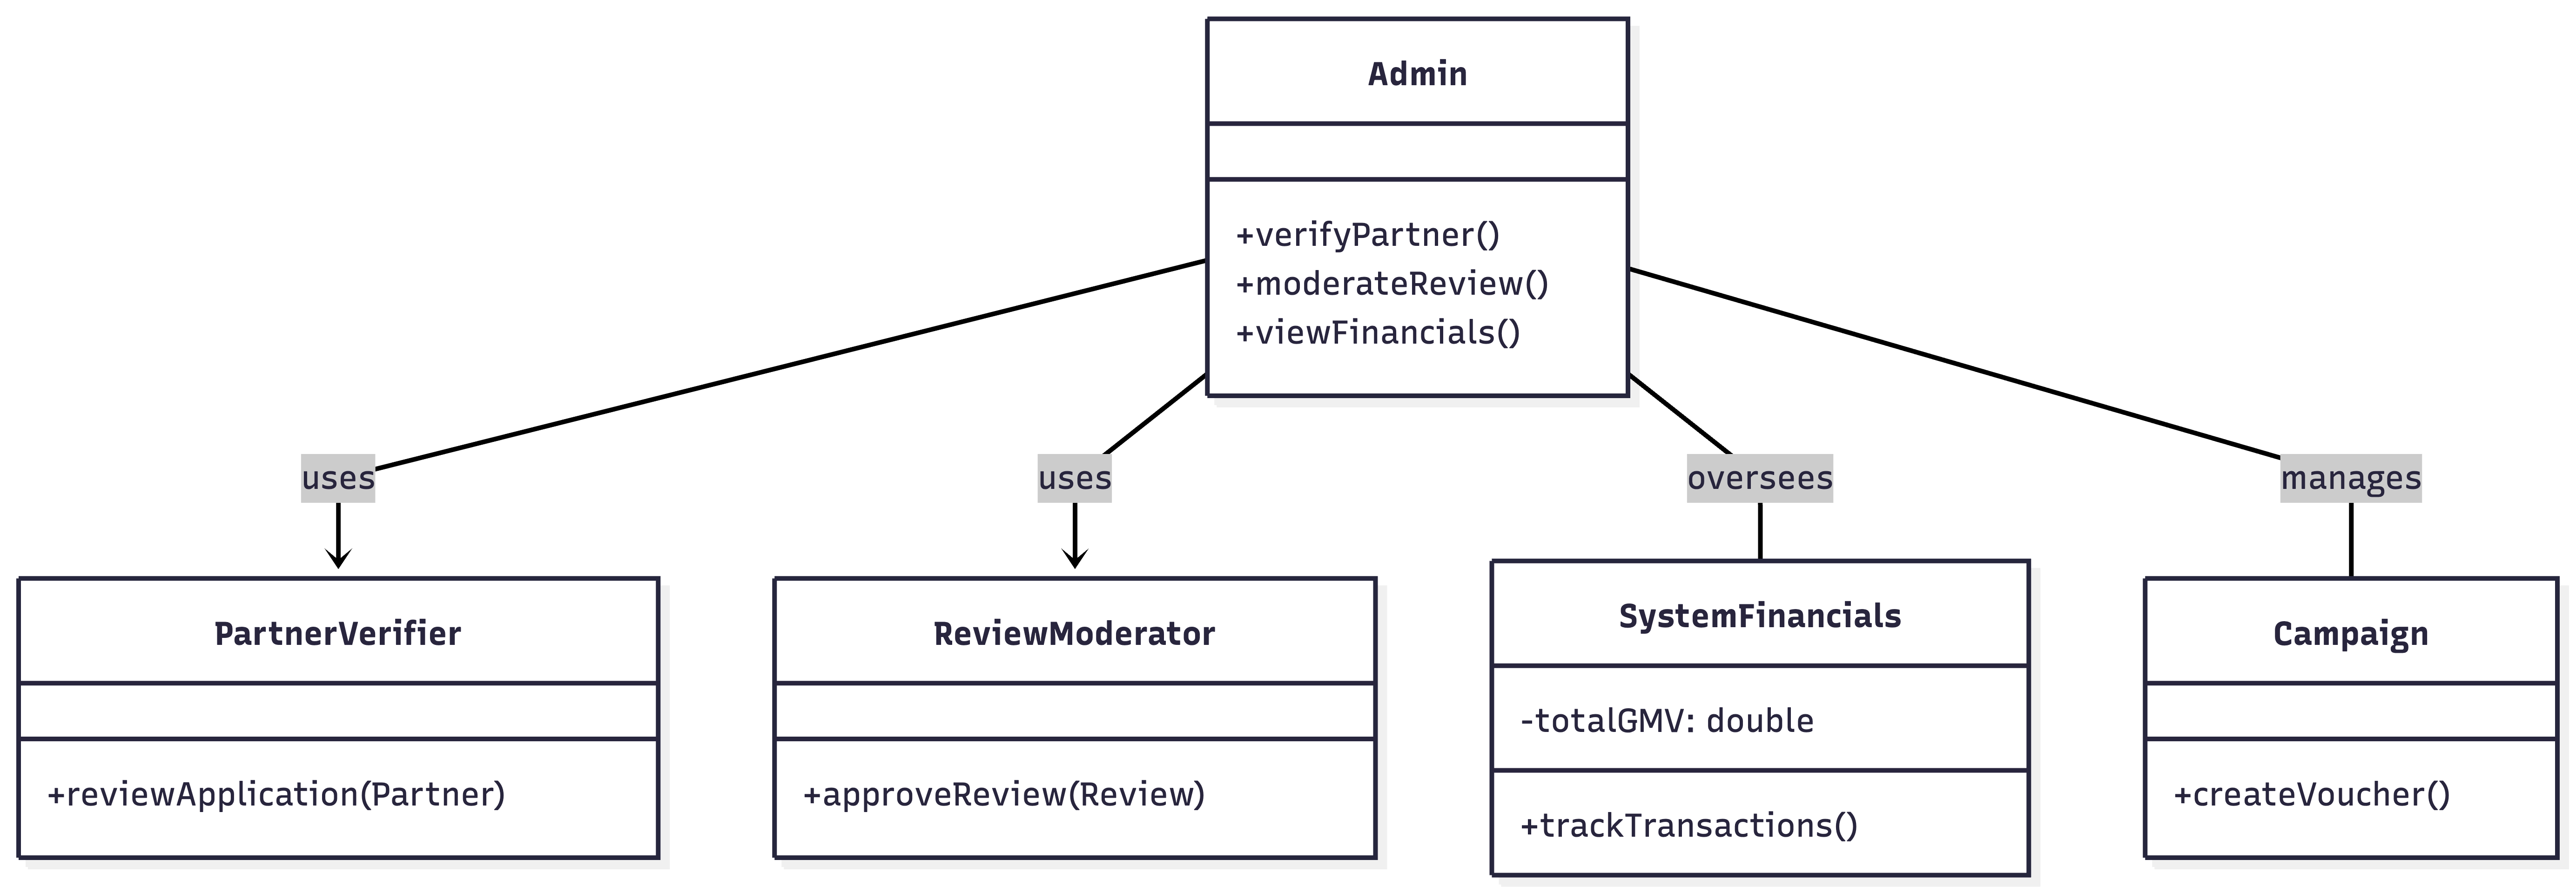
\includegraphics[width=0.8\textwidth]{Images/ClassDiagram/module_admin.png}
    \vspace{10pt}
    
    \caption{Sơ đồ lớp phân hệ Quản trị}
    \label{fig:module_admin}
\end{figure}

\subsubsubsection*{Giải thích chi tiết:}
\begin{itemize}
    \item \textbf{Facade Pattern (Implicit):} Lớp \texttt{Admin} đóng vai trò như một bề mặt chung để tương tác với các hệ thống con phức tạp (\texttt{PartnerVerifier}, \texttt{ReviewModerator}).
    \item \textbf{SystemFinancials:} Tách biệt logic tính toán doanh thu (Revenue) và tổng giá trị giao dịch (GMV) ra khỏi logic thanh toán từng đơn lẻ, tối ưu hóa cho việc báo cáo (Reporting).
    \item \textbf{Campaign Management:} Admin quản lý các chiến dịch Marketing cấp hệ thống, chứa các Voucher áp dụng toàn sàn.
\end{itemize}

% --- KẾT LUẬN ---
\subsection*{Tổng kết kiến trúc}

Sơ đồ lớp của hệ thống được thiết kế dựa trên các nguyên lý hướng đối tượng hiện đại:
\begin{enumerate}
    \item \textbf{Tính Modularity:} Các chức năng được chia tách rõ ràng.
    \item \textbf{Tính Mở rộng (Extensibility):} Sử dụng Interface và Strategy Pattern giúp dễ dàng thêm mới tính năng.
    \item \textbf{Tính Bảo mật:} Tích hợp RBAC sâu vào thiết kế lớp.
    \item \textbf{Tính Nhất quán:} Sử dụng Enum cho các trạng thái quan trọng để quản lý luồng dữ liệu.
\end{enumerate}


\newpage
\chapter{Thiết kế hệ thống}
\section{Kiến trúc tổng thể hệ thống}
\subsection{Kiến trúc N-tier}
\textbf{N-tier Architecture} (Kiến trúc đa tầng) là mô hình thiết kế phần mềm trong đó hệ thống được chia thành các tầng (layers) riêng biệt về mặt logic và vật lý.
\begin{itemize}
    \item \textbf{Nguyên tắc cốt lõi:} "Separation of Concerns" (Phân tách mối quan tâm). Mỗi tầng đảm nhiệm một chức năng cụ thể và chỉ giao tiếp với các tầng liền kề (thường là tầng ngay bên dưới nó).
    \item \textbf{Mục tiêu:} Giúp hệ thống dễ quản lý, dễ bảo trì, tăng tính bảo mật và khả năng mở rộng linh hoạt.
\end{itemize}
\subsection{Kết cấu chi tiết 5 Tầng (Structure)}
\subsubsection{Tầng 1: Presentation Layer (Client Layer)}
Đây là tầng giao diện người dùng, nơi tương tác trực tiếp với người dùng cuối (End-user).
\begin{itemize}
    \item \textbf{Chức năng:} Hiển thị thông tin và thu thập hành động của người dùng (click, nhập liệu). Nó không chứa logic nghiệp vụ phức tạp mà chỉ chịu trách nhiệm về UX/UI.
    \item \textbf{Thành phần:} Mobile App (iOS, Android, Flutter), Web App (React, Vue, Angular), hoặc Desktop App.
    \item \textbf{Giao tiếp:} Gửi yêu cầu (Request) xuống Tầng 2 và nhận phản hồi (Response) để hiển thị.
\end{itemize}
\subsubsection{Tầng 2: Connection \& API Layer (Gateway)}
Đây là "người gác cổng" (Gatekeeper) của hệ thống phía sau. Mọi yêu cầu từ Client phải đi qua đây trước khi vào hệ thống nội bộ.
\begin{itemize}
    \item \textbf{Chức năng:} \textbf{API Gateway:} Định tuyến (Routing) yêu cầu đến đúng service xử lý. \textbf{Security:} Xác thực (Authentication), Phân quyền (Authorization), chặn DDoS, Rate Limiting (giới hạn số lượt truy cập). \textbf{Load Balancing:} Cân bằng tải để phân phối request đều đặn.
    \item \textbf{Công nghệ:} NGINX, Kong, AWS API Gateway, Spring Cloud Gateway.
\end{itemize}
\subsubsection{Tầng 3: Business Logic Layer (Server Layer - Microservices)}
Đây là "bộ não" của hệ thống, nơi xử lý các quy trình nghiệp vụ chính. Trong kiến trúc hiện đại, tầng này thường được chia nhỏ thành các \textbf{Microservices}.
\begin{itemize}
    \item \textbf{Chức năng:} Xử lý tính toán, logic nghiệp vụ (ví dụ: tính toán giỏ hàng, kiểm tra tồn kho, xử lý workflow).
    \item \textbf{Đặc điểm:} Mỗi Microservice chạy độc lập, có thể viết bằng các ngôn ngữ khác nhau (Java, Go, Python, Node.js) và giao tiếp với nhau qua HTTP/REST hoặc gRPC.
    \item \textbf{Giao tiếp:} Nhận lệnh từ Tầng 2, gọi xuống Tầng 4 để lấy dữ liệu, hoặc gọi sang Tầng 5 để dùng dịch vụ bên ngoài.
\end{itemize}
\subsubsection{Tầng 4: Data Access Layer (Data \& Infrastructure Layer)}
Tầng này chịu trách nhiệm quản lý và lưu trữ dữ liệu bền vững. Tầng Business không bao giờ truy cập trực tiếp vào file database vật lý mà phải thông qua các cơ chế của tầng này.
\begin{itemize}
    \item \textbf{Chức năng:}
        \begin{itemize}
            \item Thực hiện các thao tác CRUD (Create, Read, Update, Delete).
            \item Trừu tượng hóa việc truy cập dữ liệu (giúp Tầng 3 không cần biết chi tiết kỹ thuật của Database).
            \item Quản lý kết nối đến Database.
           
        \end{itemize}
   \item \textbf{Thành phần:} ORM (Entity Framework, Hibernate), SQL Database (PostgreSQL, MySQL), NoSQL (MongoDB), Caching (Redis).
    
\end{itemize}
\subsubsection{Tầng 5: Integration Layer (Third-Party Integrations)}
Đây là tầng kết nối với thế giới bên ngoài, giúp hệ thống mở rộng chức năng mà không cần tự xây dựng lại từ đầu.
\begin{itemize}
    \item \textbf{Chức năng:}
    \begin{itemize}
        \item Đóng vai trò là "Adapter" để kết nối hệ thống nội bộ với các dịch vụ thuê ngoài.
        \item Xử lý việc chuyển đổi định dạng dữ liệu để phù hợp với API của đối tác.
    \end{itemize}
    \item \textbf{Thành phần:}  Payment Gateway (Stripe, Momo), SMS/Email Services (Twilio, SendGrid), Maps API, AI Services.
\end{itemize}

\subsection{Ưu điểm và Nhược điểm}
\begin{table}[htbp]
    \centering
    \caption{Ưu điểm và Nhược điểm của Kiến trúc Layer (N-tier)}
    \label{tab:ntier-comparison}
    \renewcommand{\arraystretch}{1.5} % Tăng khoảng cách giữa các dòng cho dễ đọc
    
    % Tạo bảng với 2 cột có độ rộng bằng nhau (X)
    \begin{tabularx}{\textwidth}{ | >{\raggedright\arraybackslash}X | >{\raggedright\arraybackslash}X | }
        \hline
        \textbf{Ưu điểm (Advantages)} & \textbf{Nhược điểm (Disadvantages)} \\  
        \hline
        
        \textbf{1. Khả năng mở rộng (Scalability):} \newline 
        Có thể mở rộng (scale-out) từng tầng riêng biệt. Ví dụ: Nếu Business Layer quá tải, chỉ cần thêm server cho tầng này mà không cần can thiệp vào Database hay Client. 
        & 
        \textbf{1. Độ trễ (Latency):} \newline 
        Hiệu năng có thể bị ảnh hưởng do dữ liệu phải di chuyển qua nhiều tầng (network hops) và các lớp bảo mật trước khi đến đích, chậm hơn so với kiến trúc nguyên khối. \\  
        \hline
        
        \textbf{2. Dễ bảo trì (Maintainability):} \newline 
        Nhờ nguyên tắc "Separation of Concerns", việc sửa lỗi hoặc nâng cấp công nghệ ở một tầng ít gây ảnh hưởng đến các tầng khác (Loose Coupling). 
        & 
        \textbf{2. Phức tạp trong vận hành:} \newline 
        Việc triển khai (deployment), giám sát (monitoring) và gỡ lỗi (debugging) trở nên khó khăn hơn vì hệ thống bị phân tán thành nhiều phần. \\  
        \hline
        
        \textbf{3. Bảo mật cao (Security):} \newline 
        Tầng dữ liệu (Data Layer) và Business Layer được che giấu sau Gateway. Kẻ tấn công khó tiếp cận trực tiếp vào cơ sở dữ liệu. 
        & 
        \textbf{3. Chi phí hạ tầng cao:} \newline 
        Yêu cầu nhiều tài nguyên server, chi phí quản lý mạng và license phần mềm để duy trì nhiều tầng riêng biệt. \\  
        \hline
        
        \textbf{4. Linh hoạt công nghệ:} \newline 
        Tầng Presentation có thể dùng Flutter/React, trong khi Business Layer có thể dùng song song Java, Go hoặc Python. 
        & 
        \textbf{4. Tính nhất quán dữ liệu:} \newline 
        Trong mô hình Microservices, việc đảm bảo dữ liệu đồng bộ giữa các service (Data Consistency) phức tạp hơn, cần các pattern nâng cao như Saga. \\  
        \hline
        
    \end{tabularx}
\end{table}

\subsection{Các Kiến trúc Thay thế và So sánh}
\begin{table}[htbp]
    \centering
    \caption{So sánh Kiến trúc N-tier với các Kiến trúc khác}
    \vspace{0.3cm}
    \renewcommand{\arraystretch}{1.5} % Khoảng cách dòng
    
    % --- CHỈNH SỬA TỶ LỆ CỘT TẠI ĐÂY ---
    % Tổng các hệ số hsize phải bằng 4 (số lượng cột X)
    % Cột 1: 0.8 (Tăng lên để chứa chữ Microservices/Orchestration không bị ngắt)
    % Cột 2: 0.6 (Giữ nguyên)
    % Cột 3: 1.3 (Giảm nhẹ để bù cho cột 1)
    % Cột 4: 1.3 (Giảm nhẹ để bù cho cột 1)
    \begin{tabularx}{\textwidth}{ 
        | >{\hsize=0.8\hsize\RaggedRight\arraybackslash}X 
        | >{\hsize=0.6\hsize\RaggedRight\arraybackslash}X 
        | >{\hsize=1.3\hsize\RaggedRight\arraybackslash}X 
        | >{\hsize=1.3\hsize\RaggedRight\arraybackslash}X | }
        
        \hline
        \textbf{So với} & \textbf{Tiêu chí} & \textbf{Ưu điểm N-tier} & \textbf{Nhược điểm N-tier} \\  
        \hline

        % --- CQRS ---
        \textbf{CQRS} & 
        Tách biệt Đọc/Ghi & 
        \textbf{Đơn giản:} Dùng chung model cho đọc/ghi giúp triển khai nhanh, code dễ hiểu, phù hợp đa số ứng dụng. & 
        \textbf{Hiệu năng truy vấn:} Khó tối ưu các báo cáo phức tạp so với database chuyên dụng cho việc đọc của CQRS. \\  
        \hline

        % --- Microservices ---
        \textbf{Microservices} & 
        Phạm vi triển khai & 
        \textbf{Dễ quản lý hạ tầng:} Ít phức tạp về mạng lưới. Test tích hợp (End-to-End) dễ hơn do luồng đi thẳng. & 
        \textbf{Khó scale cục bộ:} Phải scale cả tầng lớn thay vì từng service nhỏ. Khả năng cô lập lỗi kém hơn. \\  
        \hline

        % --- Orchestration ---
        \textbf{Orchestration} & 
        Quản lý quy trình & 
        \textbf{Luồng rõ ràng:} Dễ theo dõi (trace) luồng đi từ Client xuống DB. Tốt cho tác vụ đồng bộ. & 
        \textbf{Phình to Logic:} Dễ dẫn đến "Business Layer" quá tải khi quy trình nghiệp vụ trở nên chằng chịt. \\  
        \hline

        % --- MVP ---
        \textbf{MVP} & 
        Phạm vi kiến trúc & 
        \textbf{Vĩ mô:} N-tier giải quyết cấu trúc toàn hệ thống (Server/DB), trong khi MVP chỉ lo phần giao diện (UI). & 
        \textbf{Coupling:} Nếu không khéo, logic nghiệp vụ dễ bị dính chặt vào code giao diện hơn so với MVP thuần. \\  
        \hline

        % --- Event-Driven ---
        \textbf{Event-Driven} & 
        Giao tiếp & 
        \textbf{Nhất quán tức thì:} Xử lý đồng bộ giúp User biết ngay kết quả (thành công/thất bại). Dễ debug. & 
        \textbf{Chặn (Blocking):} Request phải chờ xử lý xong, dễ gây nghẽn cổ chai nếu tải cao so với xử lý ngầm. \\  
        \hline

    \end{tabularx}
\end{table}

\subsection{Diagram và Kết luận}
\begin{figure}[H]
    % Căn giữa hình ảnh
    \centering
    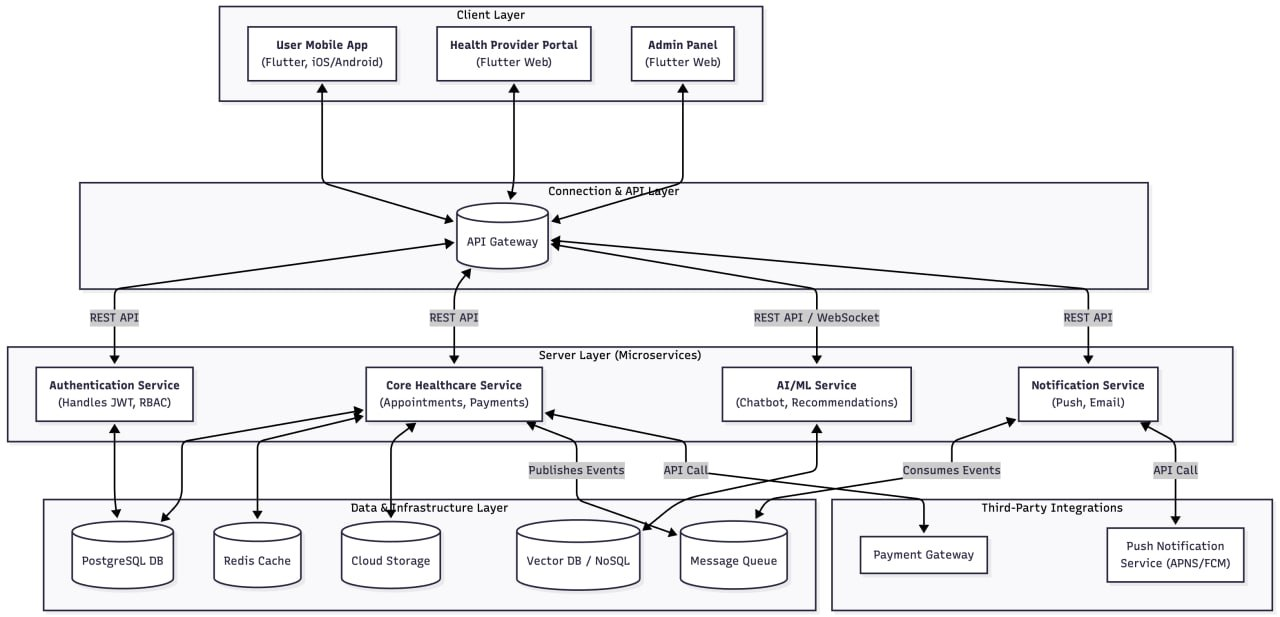
\includegraphics[width=1\textwidth]{Images/ArchSys.png}
    \vspace{10pt}
    
    % Thêm chú thích cho hình ảnh
    \caption{Kiến trúc hệ thống}
    
    % Đặt nhãn để tham chiếu chéo (cross-reference)
    \label{fig:sys_arch}
\end{figure}
Dựa trên hình ảnh \ref{fig:sys_arch}, kiến trúc tổng thể của hệ thống được thiết kế theo mô hình Microservices, chia thành 5 tầng chính (layer) với chức năng cụ thể như sau:
\begin{enumerate}
    \item \textbf{Client Layer (Tầng người dùng):}
    Đây là điểm tương tác trực tiếp với người dùng cuối và quản trị viên. Tầng này bao gồm ba ứng dụng chính được phát triển trên nền tảng Flutter:
    \begin{itemize}
        \item \textit{User Mobile App:} Ứng dụng di động (iOS/Android) dành cho khách hàng/bệnh nhân.
        \item \textit{Health Provider Portal:} Cổng thông tin dạng Web dành cho các nhà cung cấp dịch vụ y tế.
        \item \textit{Admin Panel:} Trang quản trị dạng Web để vận hành hệ thống.
    \end{itemize}

    \item \textbf{Connection \& API Layer (Tầng kết nối):}
    Đóng vai trò là cổng trung gian (Middleware) duy nhất giao tiếp giữa Client và Server.
    \begin{itemize}
        \item \textit{API Gateway:} Tiếp nhận toàn bộ yêu cầu (request) từ phía Client, thực hiện định tuyến (routing) đến các dịch vụ (services) phù hợp bên dưới.
    \end{itemize}

    \item \textbf{Server Layer (Tầng dịch vụ - Microservices):}
    Trung tâm xử lý logic nghiệp vụ, được chia nhỏ thành các dịch vụ độc lập giao tiếp qua REST API hoặc WebSocket:
    \begin{itemize}
        \item \textit{Authentication Service:} Quản lý xác thực và phân quyền (xử lý JWT, RBAC).
        \item \textit{Core Healthcare Service:} Xử lý các nghiệp vụ cốt lõi như đặt lịch khám, thanh toán. Dịch vụ này có khả năng công bố (publish) sự kiện.
        \item \textit{AI/ML Service:} Cung cấp các tính năng thông minh như Chatbot và gợi ý (Recommendations), hỗ trợ giao tiếp thời gian thực qua WebSocket.
        \item \textit{Notification Service:} Quản lý việc gửi thông báo (Push notification, Email) tới người dùng.
    \end{itemize}

    \item \textbf{Data \& Infrastructure Layer (Tầng dữ liệu và hạ tầng):}
    Nơi lưu trữ và quản lý dữ liệu bền vững, bao gồm:
    \begin{itemize}
        \item \textit{PostgreSQL DB:} Cơ sở dữ liệu quan hệ cho dữ liệu nghiệp vụ chính.
        \item \textit{Redis Cache:} Bộ nhớ đệm giúp tăng tốc độ truy xuất dữ liệu.
        \item \textit{Cloud Storage:} Lưu trữ tài liệu, hình ảnh.
        \item \textit{Vector DB / NoSQL:} Hỗ trợ lưu trữ dữ liệu phi cấu trúc phục vụ cho AI/ML.
        \item \textit{Message Queue:} Hàng đợi thông điệp giúp xử lý bất đồng bộ và giao tiếp giữa các services (Event-driven).
    \end{itemize}

    \item \textbf{Third-Party Integrations (Tầng tích hợp bên thứ ba):}
    Các dịch vụ bên ngoài được hệ thống kết nối để mở rộng tính năng:
    \begin{itemize}
        \item \textit{Payment Gateway:} Cổng thanh toán trực tuyến.
        \item \textit{Push Notification Service (APNS/FCM):} Dịch vụ đẩy thông báo của Apple và Google.
    \end{itemize}
\end{enumerate}
\section{Thiết kế cơ sở dữ liệu}
\subsection{Mô tả}
Thực thể (ERD) được cung cấp, nhằm mục đích làm rõ cấu trúc dữ liệu và các phân hệ chức năng chính của hệ thống. Mô hình dữ liệu cho thấy đây là một nền tảng công nghệ được thiết kế để kết nối ba nhóm đối tượng chính: Người dùng cuối (Khách hàng), Đối tác cung cấp dịch vụ (Partner), và Nhân viên quản trị (Employee).
\subsection{Các khối chức năng chính}
 Dựa trên các thực thể và mối quan hệ trong sơ đồ, hệ thống được cấu thành từ các khối chức năng (module) chính sau:
 \begin{itemize}
            \item Module Quản lý Tài khoản và Phân quyền (Account Management)
            Đây là module lõi, quản lý định danh và quyền truy cập của toàn bộ người dùng trên hệ thống.
            \begin{itemize}
                \item Thực thể trung tâm: \textbf{Account} lưu trữ thông tin xác thực chung
                \item Cơ chế phân quyền: Hệ thống định nghĩa ba vai trò người dùng riêng biệt với các quyền hạn khác nhau:
                \begin{itemize}
                    \item User: Đối tượng sử dụng dịch vụ.
                    \item Partner: Đối tượng cung cấp dịch vụ/sản phẩm.
                    \item Employee: Đối tượng quản trị và vận hành nền tảng.
                \end{itemize}
                \item Chức năng: Cung cấp cơ chế đăng ký, đăng nhập, xác thực và phân quyền truy cập chức năng tương ứng với từng vai trò.
            \end{itemize}
            \item \textbf{Phân hệ Vận hành dành cho Đối tác (Partner Portal)}: 
            Phân hệ này cung cấp một cổng quản trị toàn diện, cho phép các đối tác số hóa và quản lý hoạt động kinh doanh của mình.
            \begin{itemize}
                \item Quản lý Dịch vụ \& Sản phẩm (Service, Product): Cho phép đối tác khởi tạo, cấu hình giá, mô tả và phân loại các dịch vụ/sản phẩm cung cấp. Thực thể Category giúp hệ thống hóa và hỗ trợ tìm kiếm hiệu quả.
                \item Quản lý Nhân sự (Employee của Partner): Hỗ trợ đối tác quản lý thông tin nhân viên thực hiện dịch vụ.
                \item Quản lý Lịch trình (Schedule): Cung cấp công cụ thiết lập lịch làm việc cho cơ sở và từng nhân viên, làm cơ sở cho tính năng đặt lịch.
            \end{itemize}
        \item \textbf{Phân hệ Trải nghiệm Người dùng (User Experience)} Phân hệ này xây dựng luồng tương tác hoàn chỉnh cho khách hàng cuối.
            \begin{itemize}
                \item Đặt lịch (Booking): Là nghiệp vụ cốt lõi, liên kết các thực thể chính: User, Partner, Service, và Employee (của Partner) tại một thời điểm cụ thể. Trạng thái của lịch hẹn (ví dụ: chờ xác nhận, đã hoàn thành, đã hủy) cũng được quản lý tại đây.
            \item Tìm kiếm và Khám phá: Cấu trúc dữ liệu cho phép người dùng truy vấn, lọc và tìm kiếm dịch vụ/đối tác dựa trên nhiều tiêu chí.
            \item Phản hồi và Đánh giá (Feedback/Review): Sau khi sử dụng dịch vụ, người dùng có thể cung cấp phản hồi, giúp xây dựng độ tin cậy và là cơ sở để đánh giá chất lượng đối tác. 
            \end{itemize}
        \item \textbf{Module Tài chính và Marketing}
        Module này tích hợp các nghiệp vụ liên quan đến giao dịch và các hoạt động thu hút người dùng.
            \begin{itemize}
                \item Xử lý Thanh toán (Payment): Mỗi thực thể Booking được liên kết với một giao dịch Payment, ghi nhận các thông tin về số tiền, phương thức và trạng thái thanh toán.
                \item Quản lý Khuyến mãi (Promotion\(\)Voucher): Cung cấp chức năng tạo và quản lý các chương trình khuyến mãi. Các chương trình này có thể được áp dụng vào giao dịch Booking để điều chỉnh giá trị thanh toán cuối cùng.
            \end{itemize}
        \end{itemize}
\subsection{Kết luận}
Sơ đồ ERD mô tả một cấu trúc dữ liệu chặt chẽ và toàn diện cho một nền tảng dịch vụ đa năng. Từ phân tích trên, có thể xác định các năng lực chính của hệ thống bao gồm:
    \begin{itemize}
        \item Hệ thống quản lý người dùng đa vai trò với cơ chế phân quyền rõ ràng.
        \item Nền tảng đặt lịch (booking platform) thông minh, kết nối nhu cầu của người dùng với khả năng cung ứng của đối tác.
        \item Cổng quản trị dành cho đối tác (partner portal) để tự quản lý vận hành kinh doanh.
        \item Cơ chế thanh toán và khuyến mãi tích hợp, hỗ trợ hoàn chỉnh vòng đời giao dịch và các hoạt động marketing.
        \item Hệ thống thu thập phản hồi và đánh giá, đảm bảo chất lượng và tính minh bạch của nền tảng.
    \end{itemize}
\subsection{Lược đồ}
\begin{figure}[H]
    % Căn giữa hình ảnh
    \centering
    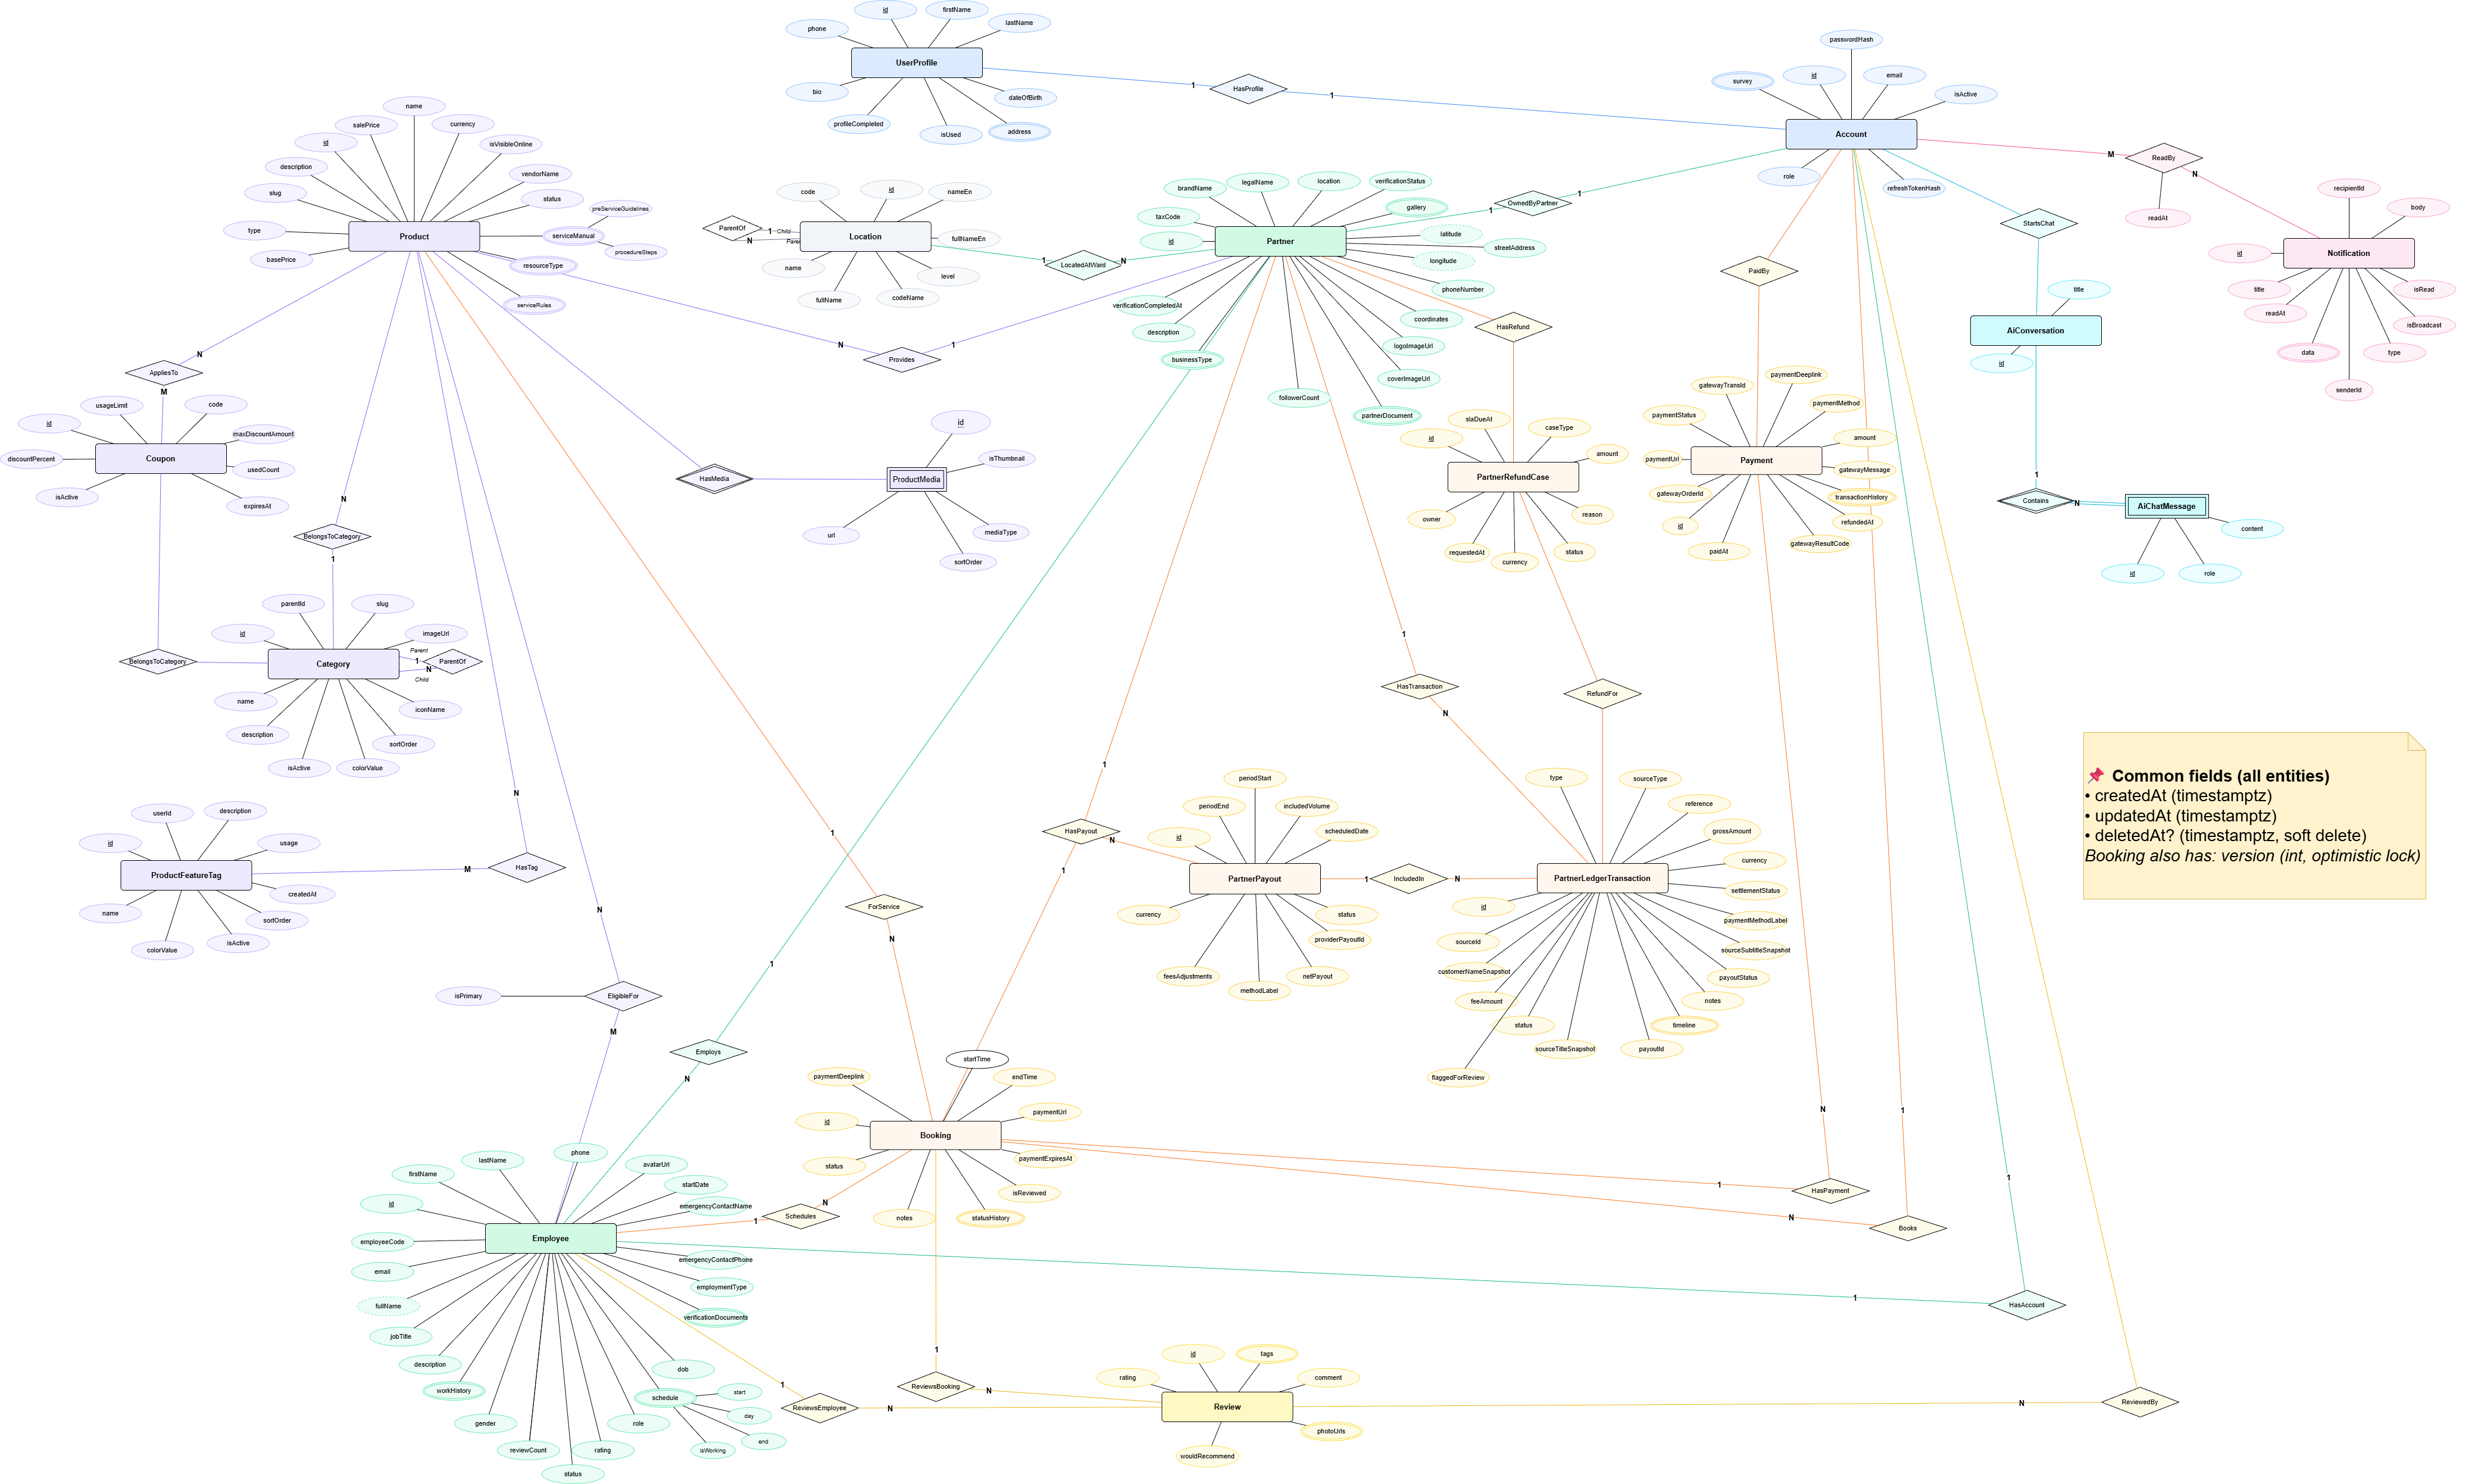
\includegraphics[angle=-90, width=0.6\textwidth]{Images/ERD.png}
    \vspace{10pt}
    
    % Thêm chú thích cho hình ảnh
    \caption{ER Diagram của hệ thống}
    
    % Đặt nhãn để tham chiếu chéo (cross-reference)
    \label{fig:erd}
\end{figure}


\section{Thiết kế UI/UX cơ bản}

\subsection{Mockup UI - Tổng quan giao diện}
Sơ đồ mockup UI dưới đây thể hiện tổng quan luồng điều hướng và các màn hình chính của ứng dụng di động Healytics. Wireframe này được thiết kế để minh họa trải nghiệm người dùng từ khi đăng nhập cho đến khi sử dụng các tính năng cốt lõi của hệ thống.

\begin{figure}[H]
    \centering
    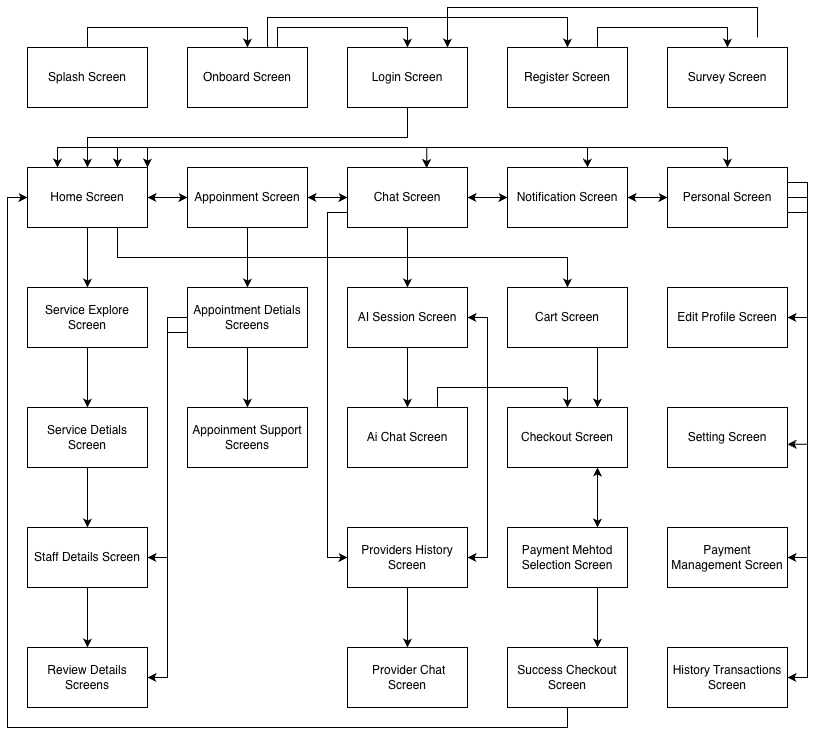
\includegraphics[width=1\textwidth]{Images/uiux/mock_ui.drawio.png}
    \vspace{10pt}
    \caption{Sơ đồ Mockup UI tổng quan của ứng dụng}
    \label{fig:mockup_ui_overview}
\end{figure}

Mockup bao gồm các nhóm màn hình chính:
\begin{itemize}
    \item \textbf{Authentication Flow:} Luồng xác thực bao gồm các màn hình đăng nhập, đăng ký qua email, xác thực OTP và các bước điền thông tin cá nhân.
    \item \textbf{Survey Flow:} Chuỗi các bước khảo sát thu thập thông tin sức khỏe và sở thích của người dùng để cá nhân hóa trải nghiệm.
    \item \textbf{Main Navigation:} Các màn hình điều hướng chính bao gồm Trang chủ (Home), Khám phá dịch vụ (Explore), Thông báo (Notification), và Trang cá nhân (Profile).
    \item \textbf{Appointment Booking:} Luồng đặt lịch hẹn khám bệnh với các bước chọn dịch vụ, thời gian, và xác nhận thông tin.
    \item \textbf{Provider \& Service Details:} Các màn hình hiển thị thông tin chi tiết về nhà cung cấp dịch vụ y tế và các dịch vụ cụ thể.
    \item \textbf{AI Chat Assistant:} Giao diện trợ lý AI hỗ trợ người dùng tư vấn sức khỏe thông qua hội thoại tự nhiên.
\end{itemize}

Các phần tiếp theo trình bày chi tiết thiết kế giao diện cho các nhóm chức năng cốt lõi. Các nhóm chức năng bổ sung (Survey, Provider Service, Checkout) được trình bày đầy đủ tại \textbf{Phụ lục A}.

\subsection{Authentication - Đăng nhập \& Đăng ký}
\begin{figure}[H]
    \centering
    
    % --- Hàng 1 ---
    \begin{subfigure}[b]{0.24\textwidth}
        \centering
        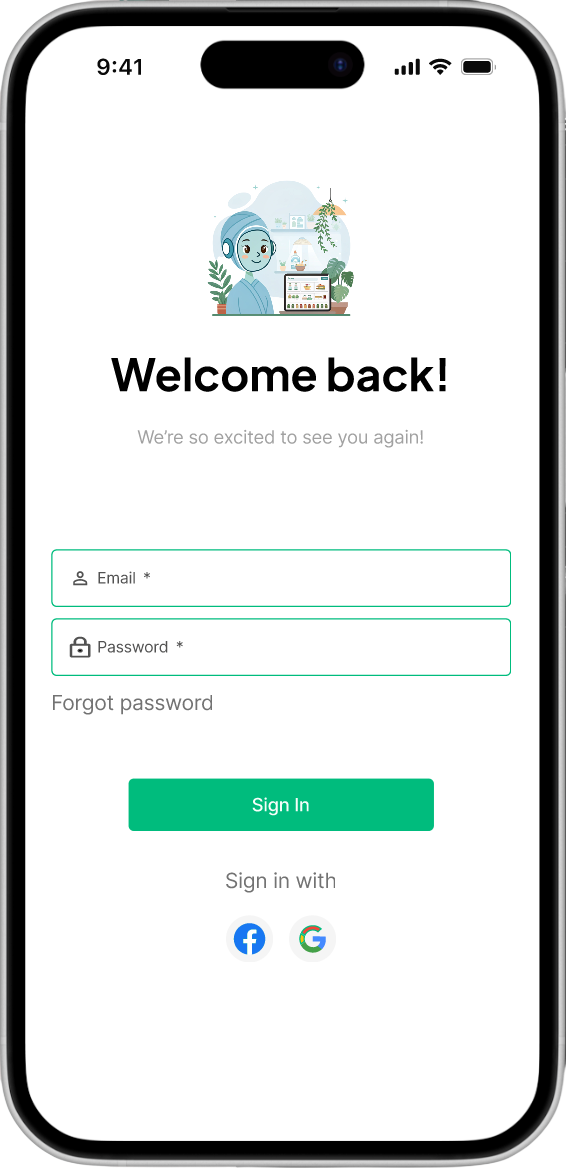
\includegraphics[width=\linewidth]{Images/uiux/authen/login.png}
        \caption{Login Page}
    \end{subfigure}
    \hfill
    \begin{subfigure}[b]{0.24\textwidth}
        \centering
        
\includegraphics[width=\linewidth]{Images/uiux/authen/signup_email.png}
        \caption{Sign Up Email}
    \end{subfigure}
    \hfill
    \begin{subfigure}[b]{0.24\textwidth}
        \centering
        
\includegraphics[width=\linewidth]{Images/uiux/authen/signup_otp.png}
        \caption{Sign Up OTP}
    \end{subfigure}
    \hfill
    \begin{subfigure}[b]{0.24\textwidth}
        \centering
        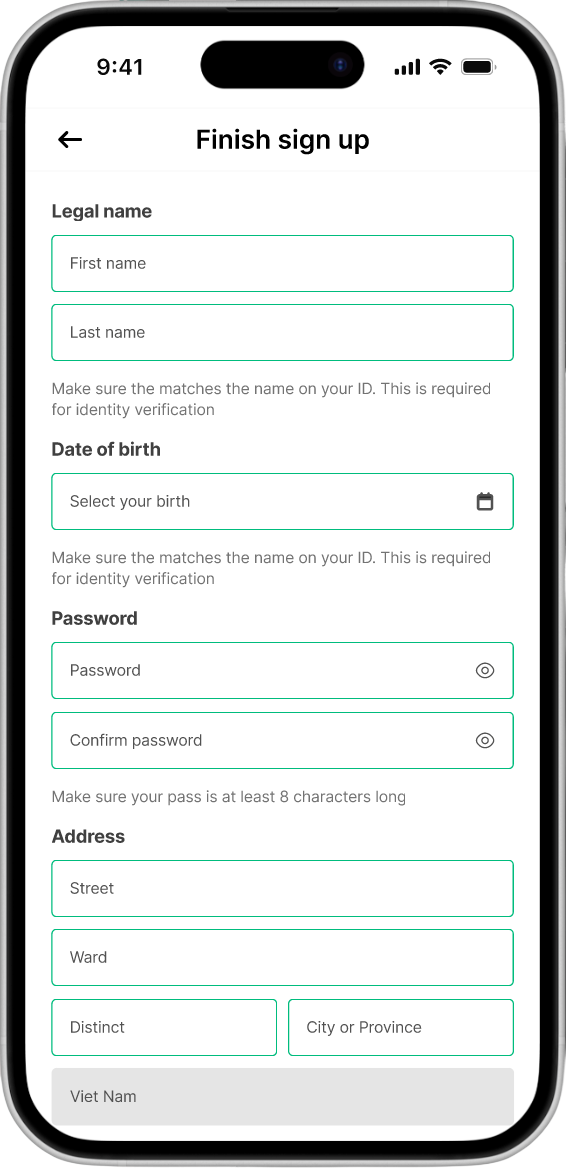
\includegraphics[width=\linewidth]{Images/uiux/authen/signup_form1.png}
        \caption{Sign Up Form 1}
    \end{subfigure}
    
    \vspace{1em}
    
    % --- Hàng 2 ---
    \begin{subfigure}[b]{0.24\textwidth}
        \centering
        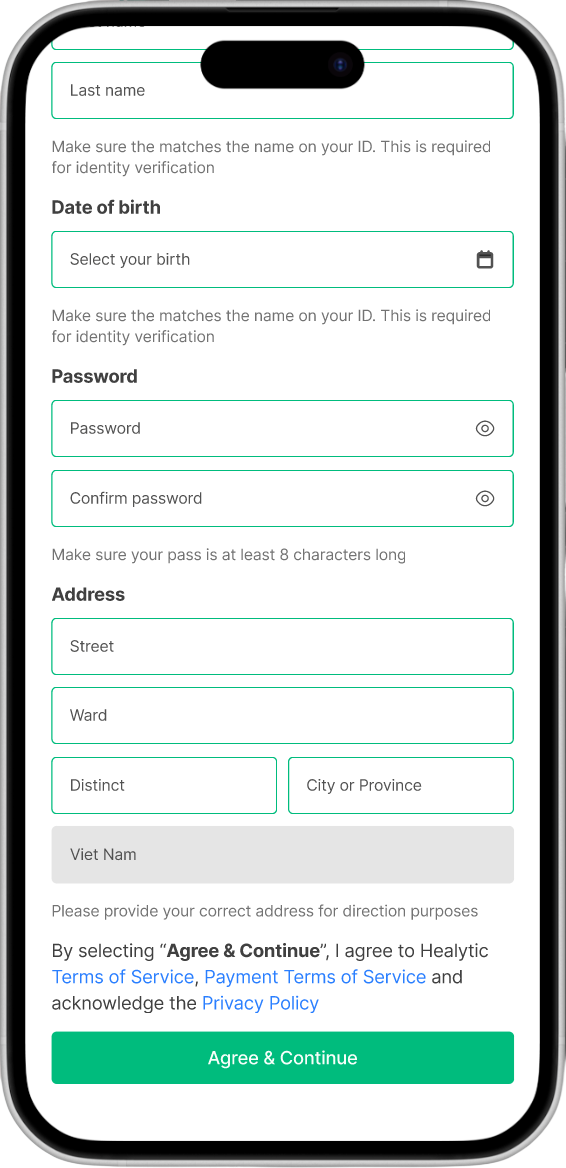
\includegraphics[width=\linewidth]{Images/uiux/authen/signup_form2.png}
        \caption{Sign Up Form 2}
    \end{subfigure}
    \hfill
    \begin{subfigure}[b]{0.24\textwidth}
        \centering
        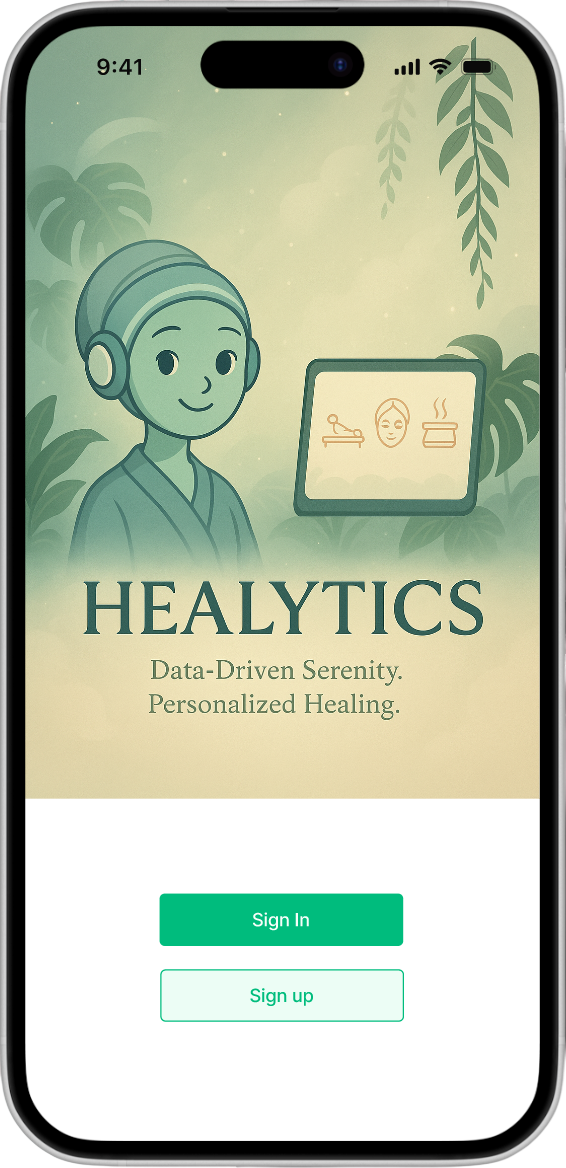
\includegraphics[width=\linewidth]{Images/uiux/authen/dashboard.png}
        \caption{Dashboard}
    \end{subfigure}
    \hfill
    \begin{subfigure}[b]{0.24\textwidth}
    \end{subfigure}
    \hfill
    \begin{subfigure}[b]{0.24\textwidth}
    \end{subfigure}
    
    \vspace{1em}
    \caption{Giao diện Authentication}
\end{figure}

\subsection{Navigation - Các trang điều hướng chính}
\begin{figure}[H]
    \centering
    
    % --- Hàng 1 ---
    \begin{subfigure}[b]{0.24\textwidth}
        \centering
        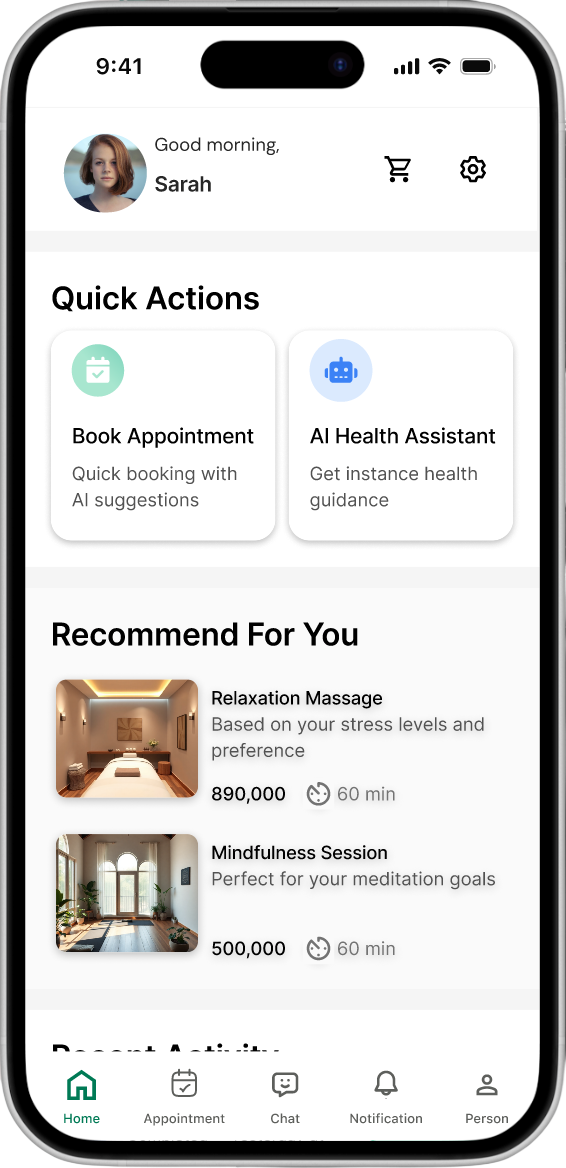
\includegraphics[width=\linewidth]{Images/uiux/navigation/home_1.png}
        \caption{Home Page 1}
    \end{subfigure}
    \hfill
    \begin{subfigure}[b]{0.24\textwidth}
        \centering
        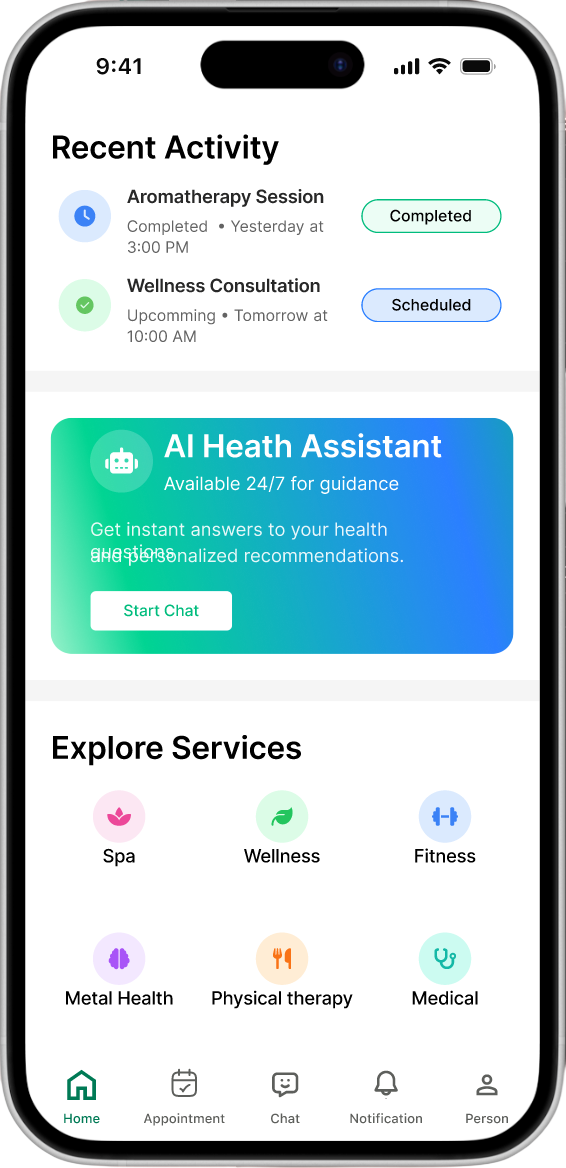
\includegraphics[width=\linewidth]{Images/uiux/navigation/home_2.png}
        \caption{Home Page 2}
    \end{subfigure}
    \hfill
    \begin{subfigure}[b]{0.24\textwidth}
        \centering
        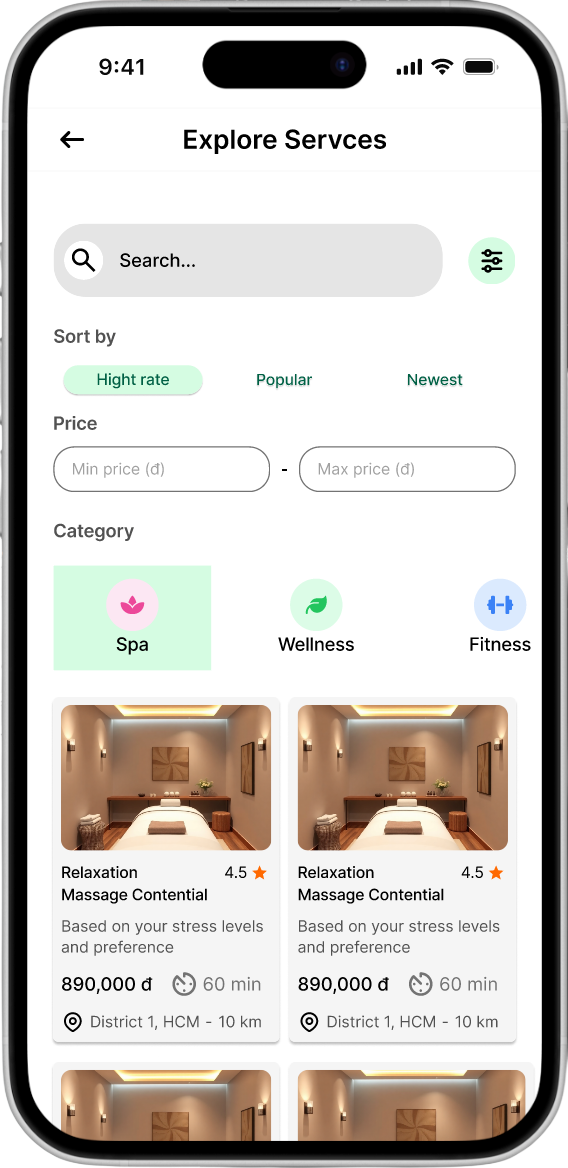
\includegraphics[width=\linewidth]{Images/uiux/navigation/explore_service.png}
        \caption{Explore Services}
    \end{subfigure}
    \hfill
    \begin{subfigure}[b]{0.24\textwidth}
        \centering
        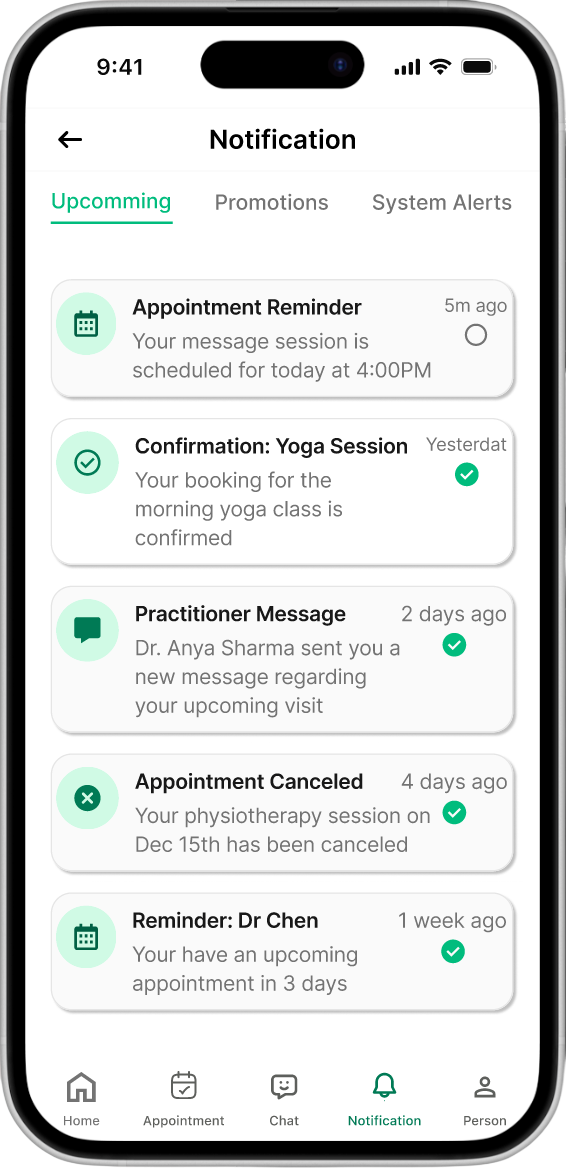
\includegraphics[width=\linewidth]{Images/uiux/navigation/notification.png}
        \caption{Notification}
    \end{subfigure}
    
    \vspace{1em}
    
    % --- Hàng 2 ---
    \begin{subfigure}[b]{0.24\textwidth}
        \centering
        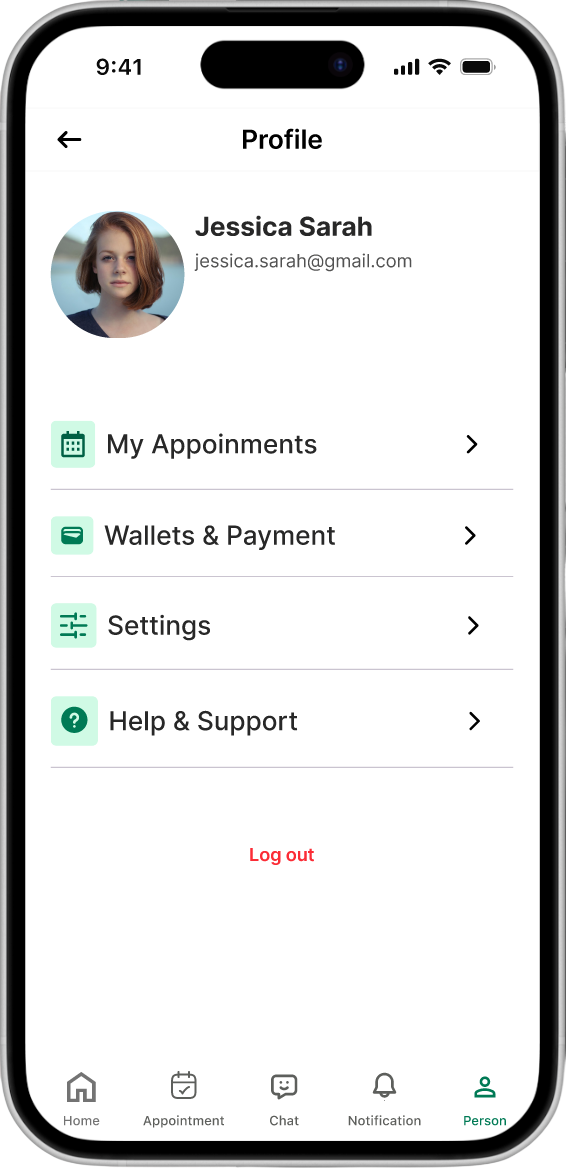
\includegraphics[width=\linewidth]{Images/uiux/navigation/personal.png}
        \caption{Personal Profile}
    \end{subfigure}
    \hfill
    \begin{subfigure}[b]{0.24\textwidth}
        \centering
        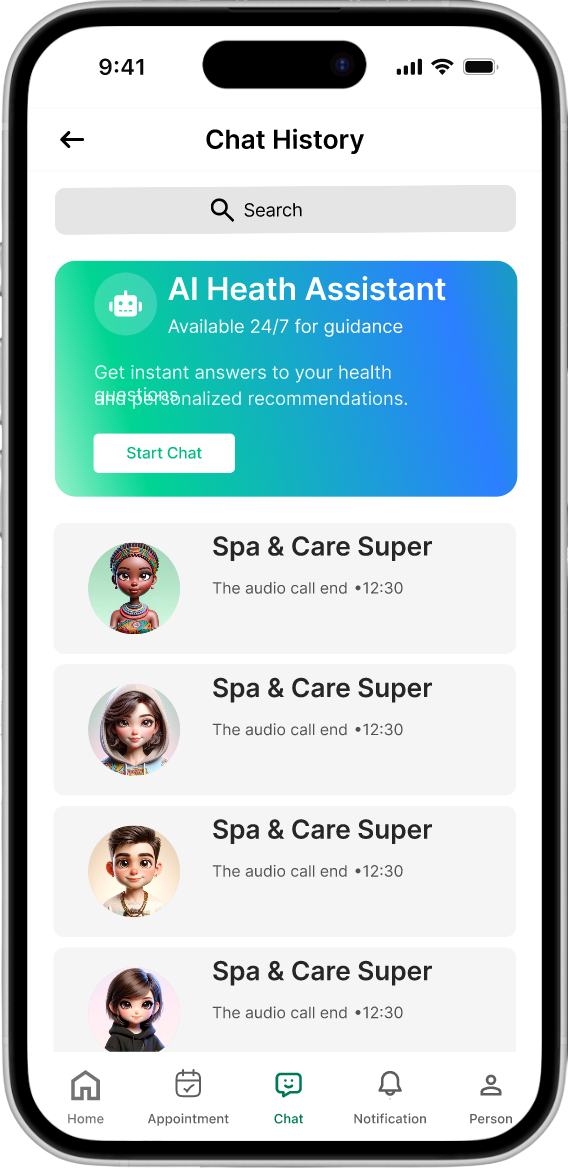
\includegraphics[width=\linewidth]{Images/uiux/navigation/chat_history.png}
        \caption{Chat History}
    \end{subfigure}
    \hfill
    \begin{subfigure}[b]{0.24\textwidth}
        \centering
        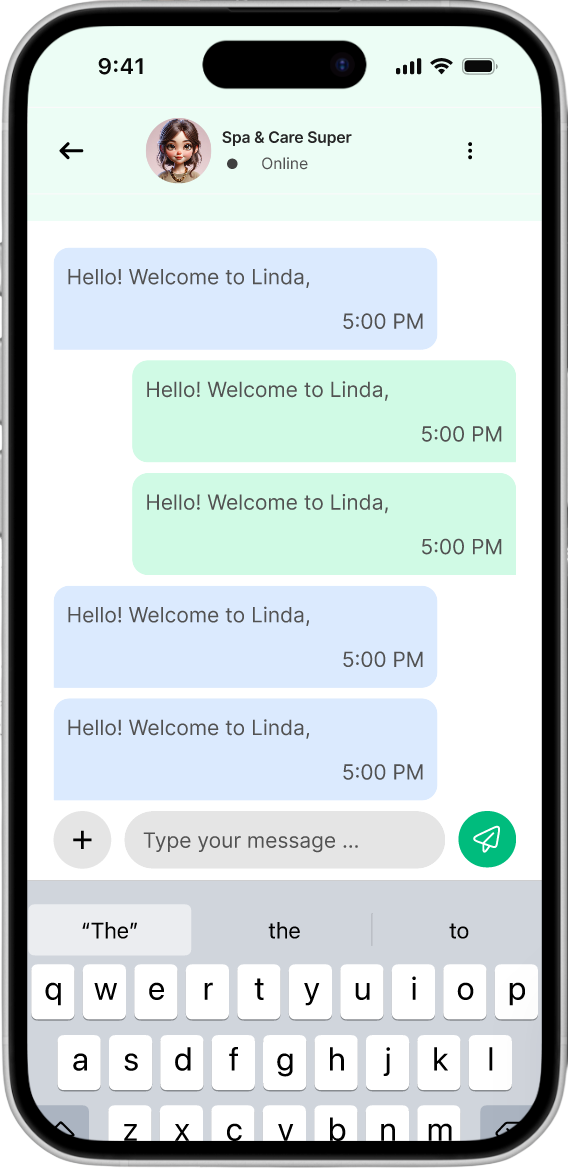
\includegraphics[width=\linewidth]{Images/uiux/navigation/chat_box.png}
        \caption{Chat Box}
    \end{subfigure}
    \hfill
    \begin{subfigure}[b]{0.24\textwidth}
    \end{subfigure}
    
    \vspace{1em}
    \caption{Giao diện Navigation}
\end{figure}

\subsection{Appointment - Đặt lịch hẹn}
\begin{figure}[H]
    \centering
    
    % --- Hàng 1 ---
    \begin{subfigure}[b]{0.24\textwidth}
        \centering
        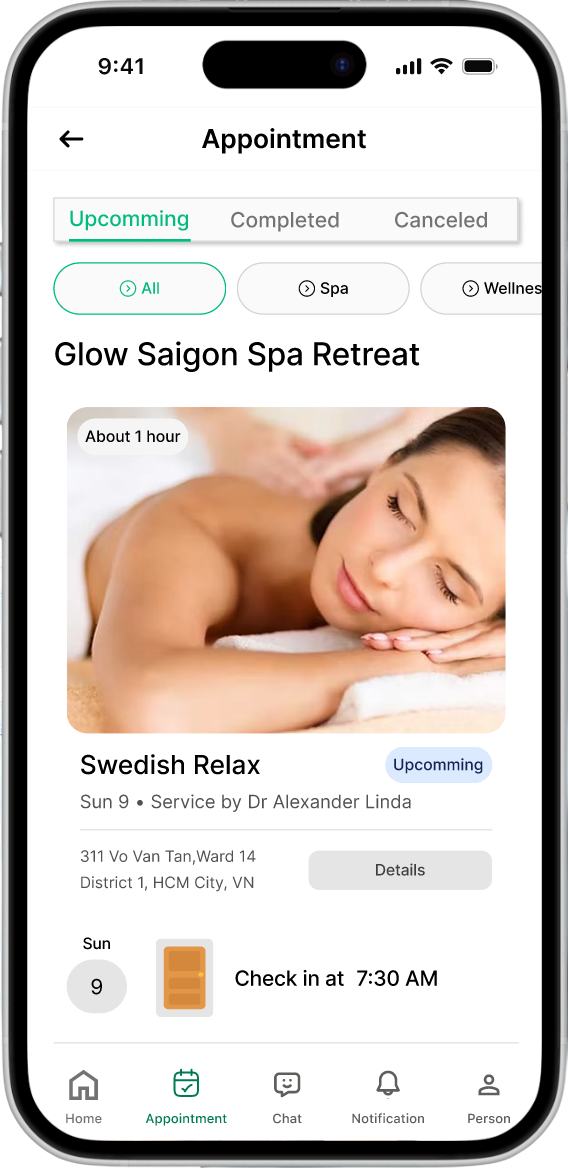
\includegraphics[width=\linewidth]{Images/uiux/appointment/appointment_1.png}
        \caption{Appointment Step 1}
    \end{subfigure}
    \hfill
    \begin{subfigure}[b]{0.24\textwidth}
        \centering
        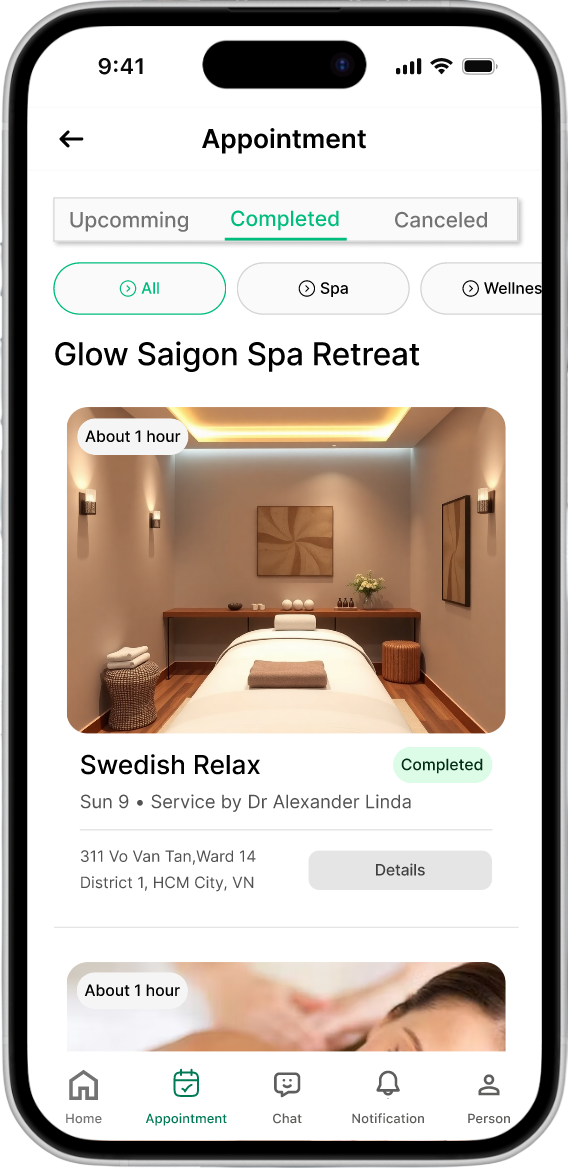
\includegraphics[width=\linewidth]{Images/uiux/appointment/appointment_2.png}
        \caption{Appointment Step 2}
    \end{subfigure}
    \hfill
    \begin{subfigure}[b]{0.24\textwidth}
        \centering
        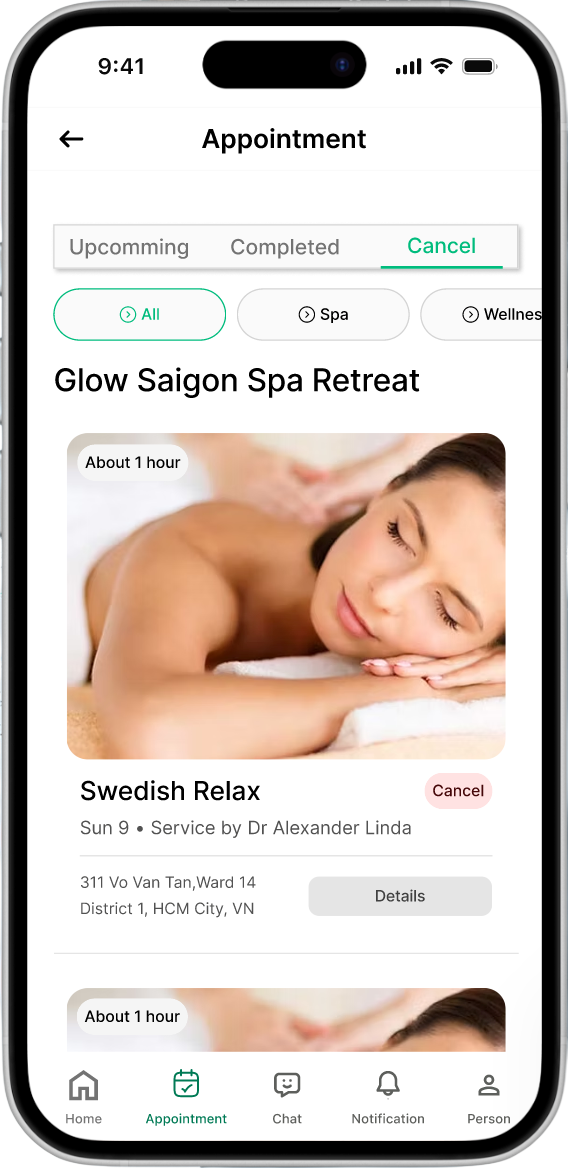
\includegraphics[width=\linewidth]{Images/uiux/appointment/appointment_3.png}
        \caption{Appointment Step 3}
    \end{subfigure}
    \hfill
    \begin{subfigure}[b]{0.24\textwidth}
        \centering
        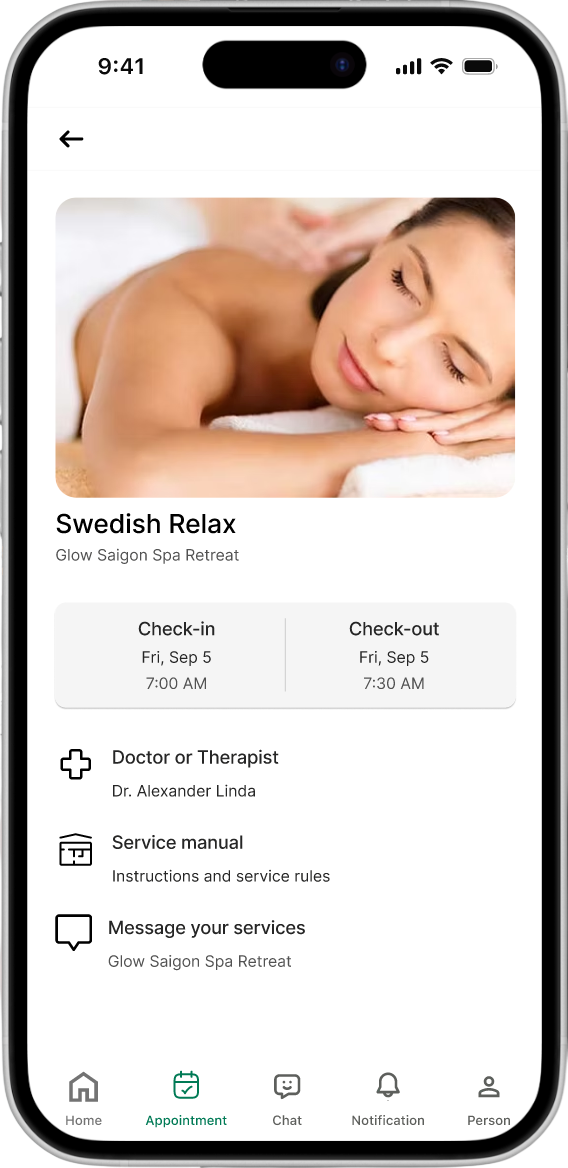
\includegraphics[width=\linewidth]{Images/uiux/appointment/appointment_details.png}
        \caption{Appointment Details}
    \end{subfigure}
    
    \vspace{1em}
    
    % --- Hàng 2 ---
    \begin{subfigure}[b]{0.24\textwidth}
        \centering
        
\includegraphics[width=\linewidth]{Images/uiux/appointment/doctor_detail.png}
        \caption{Doctor Detail}
    \end{subfigure}
    \hfill
    \begin{subfigure}[b]{0.24\textwidth}
        \centering
        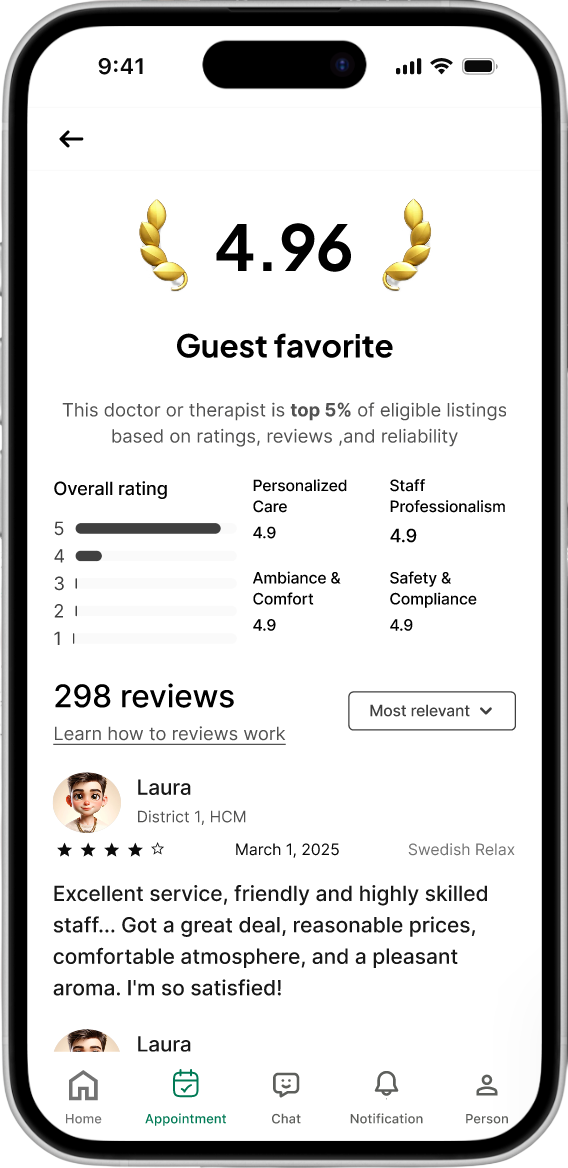
\includegraphics[width=\linewidth]{Images/uiux/appointment/review_detail.png}
        \caption{Review Detail}
    \end{subfigure}
    \hfill
    \begin{subfigure}[b]{0.24\textwidth}
    \end{subfigure}
    \hfill
    \begin{subfigure}[b]{0.24\textwidth}
    \end{subfigure}
    
    \vspace{1em}
    \caption{Giao diện Appointment}
\end{figure}

\subsection{AI Chat - Trợ lý AI}
\begin{figure}[H]
    \centering
    
    % --- Hàng 1 ---
    \begin{subfigure}[b]{0.24\textwidth}
        \centering
        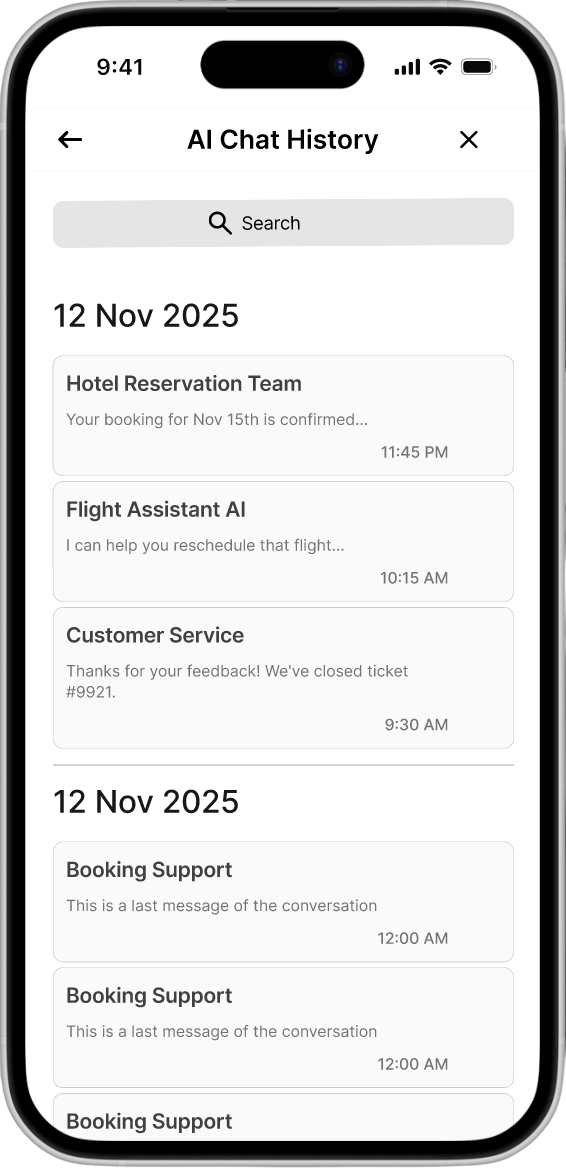
\includegraphics[width=\linewidth]{Images/uiux/ai_chat/aichat_session.png}
        \caption{AI Chat Session}
    \end{subfigure}
    \hfill
    \begin{subfigure}[b]{0.24\textwidth}
        \centering
        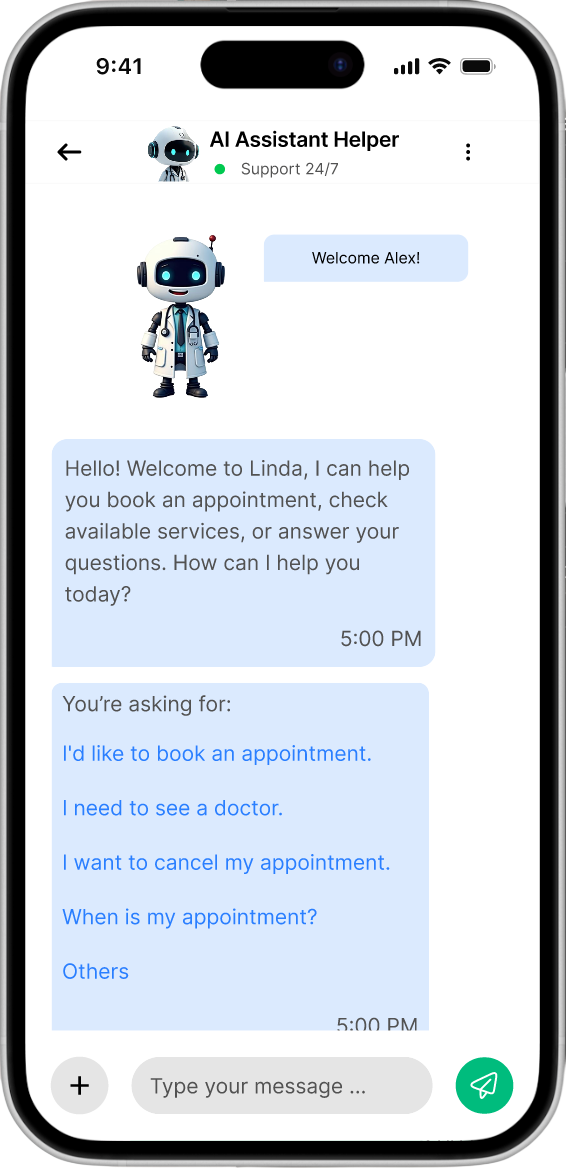
\includegraphics[width=\linewidth]{Images/uiux/ai_chat/aichat_box_1.png}
        \caption{AI Chat Box 1}
    \end{subfigure}
    \hfill
    \begin{subfigure}[b]{0.24\textwidth}
        \centering
        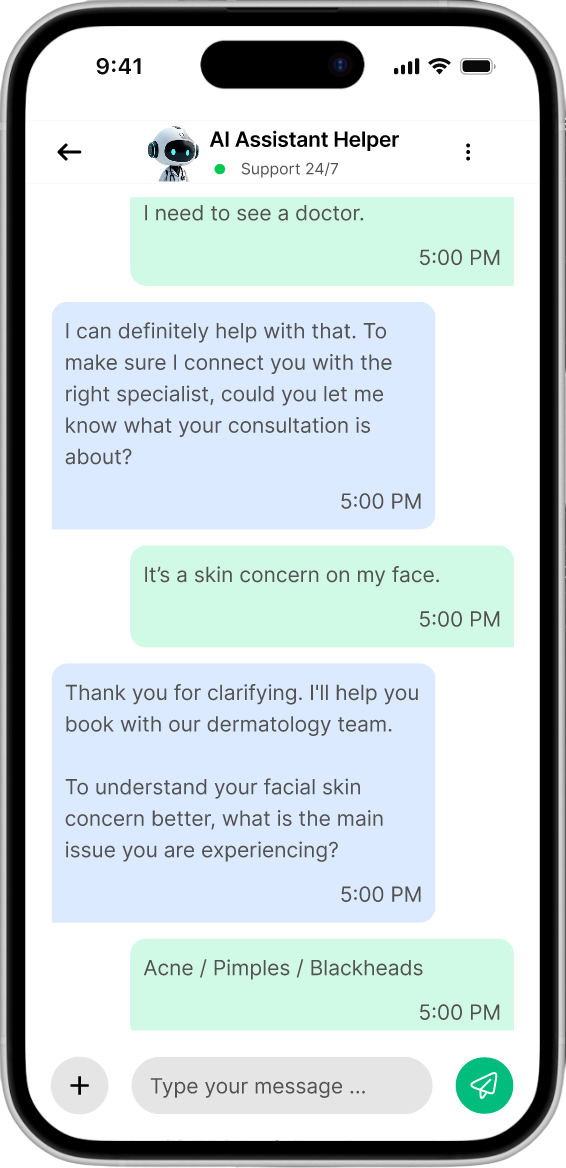
\includegraphics[width=\linewidth]{Images/uiux/ai_chat/aichat_box_2.png}
        \caption{AI Chat Box 2}
    \end{subfigure}
    \hfill
    \begin{subfigure}[b]{0.24\textwidth}
        \centering
        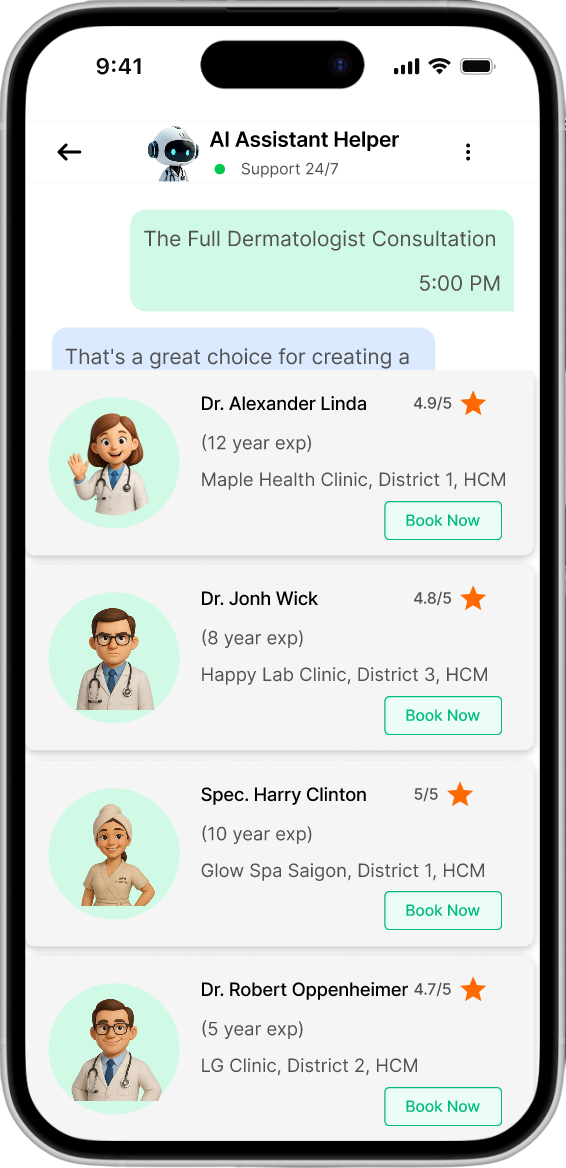
\includegraphics[width=\linewidth]{Images/uiux/ai_chat/aichat_box_3.png}
        \caption{AI Chat Box 3}
    \end{subfigure}
    
    \vspace{1em}
    
    % --- Hàng 2 ---
    \begin{subfigure}[b]{0.24\textwidth}
        \centering
        
\includegraphics[width=\linewidth]{Images/uiux/ai_chat/aichat_box_4.png}
        \caption{AI Chat Box 4}
    \end{subfigure}
    \hfill
    \begin{subfigure}[b]{0.24\textwidth}
        \centering
        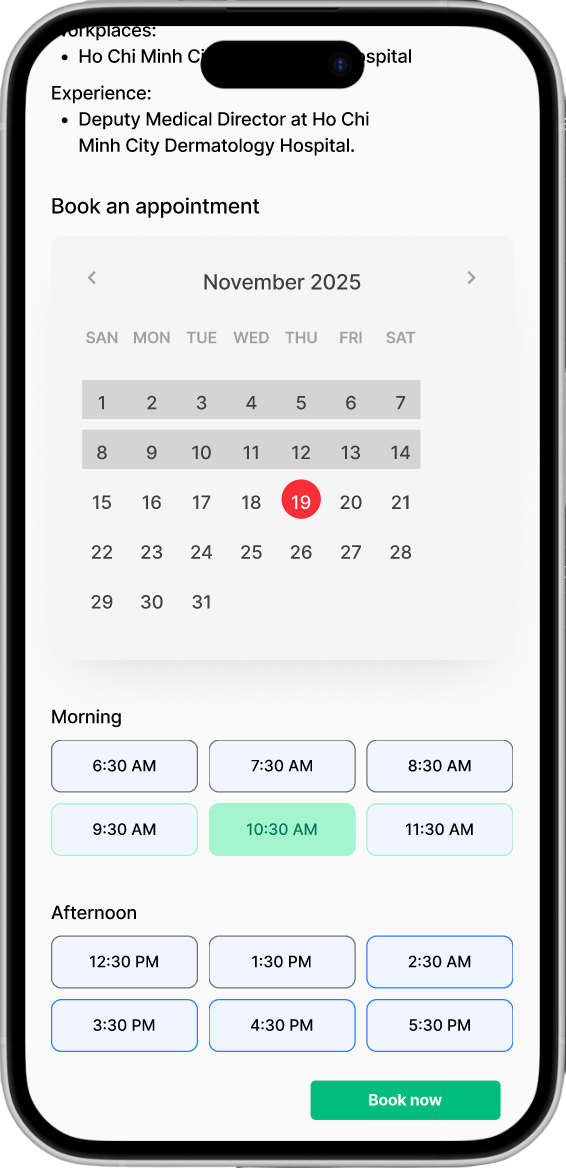
\includegraphics[width=\linewidth]{Images/uiux/ai_chat/aichat_box_5.png}
        \caption{AI Chat Box 5}
    \end{subfigure}
    \hfill
    \begin{subfigure}[b]{0.24\textwidth}
    \end{subfigure}
    \hfill
    \begin{subfigure}[b]{0.24\textwidth}
    \end{subfigure}
    
    \vspace{1em}
    \caption{Giao diện AI Chat}
\end{figure}

\section{Phần AI – Thiết kế}
\subsection{Thu thập và tiền xử lý dữ liệu}

Dữ liệu phục vụ các pipeline AI trong mã nguồn hiện tại được phân theo từng dịch vụ như sau.

\begin{itemize}
    \item \textbf{RAG Chatbot:} Kho tri thức gồm các tài liệu PDF; khi khởi động dịch vụ, toàn bộ PDF trong thư mục tri thức được đọc song song, loại bỏ ký tự ngoài ASCII (UTF-8), sau đó chia nhỏ bằng \textit{Recursive Character Text Splitter} với độ dài đoạn 300 ký tự và không chồng lấp giữa các đoạn.
    \item \textbf{Recommender (vector search):} Danh mục dịch vụ nguồn đọc từ tệp JSON; mỗi bản ghi được ghép thành một văn bản gồm tên và mô tả, gắn metadata \texttt{service\_id} và \texttt{category}, rồi được embedding và lưu vào Chroma persistent để truy vấn tương đồng.
    \item \textbf{Recommender Home (hồ sơ người dùng):} Dịch vụ gợi ý trang chủ đọc PostgreSQL: khảo sát người dùng lưu trong trường JSON trên bảng tài khoản (chuẩn hóa thành ba nhóm \textit{goals}, \textit{interests}, \textit{health\_conditions}), đồng thời có thể đọc hồ sơ cá nhân (tên, ngày sinh suy ra tuổi, v.v.). Danh sách mã dịch vụ đã dùng được dự kiến lấy từ lịch sử đơn hàng nhưng trong triển khai hiện tại luôn trả về rỗng cho đến khi tích hợp bảng đơn hàng.
    \item \textbf{NER / PreFilter:} Dịch vụ tải cache địa điểm và dữ liệu phục vụ lọc từ cơ sở dữ liệu quan hệ khi khởi động; hỗ trợ truy vấn không gian (PostGIS) khi có ngữ cảnh khoảng cách hợp lệ.
\end{itemize}

\subsection{Thiết kế hệ thống NER/PreFilter}

\subsubsection{Mục tiêu thiết kế và vai trò trong pipeline}

NER Service được thiết kế như một vi dịch vụ độc lập để tiếp nhận truy vấn ngôn ngữ tự nhiên, trích xuất thực thể và chuyển đổi thành điều kiện lọc cho tầng gợi ý. Trong pipeline hội thoại, dịch vụ này đóng vai trò \textit{pre-filtering gate}: giảm không gian tìm kiếm của recommender trước khi đưa vào bước xếp hạng ngữ nghĩa.

Các endpoint chính gồm:
\begin{itemize}
    \item \texttt{/ner/extract}: trả danh sách thực thể đã chuẩn hóa.
    \item \texttt{/prefilter/search}: chạy luồng extract $\rightarrow$ normalize $\rightarrow$ spatial filter và trả danh sách \texttt{service\_id} phù hợp.
\end{itemize}

\subsubsection{Kiến trúc Hybrid NER}

Hệ thống áp dụng kiến trúc lai (Hybrid NER), kết hợp nhiều kỹ thuật để cân bằng giữa độ chính xác và tính ổn định vận hành:
\begin{itemize}
    \item \textbf{LLM-based extraction (Gemini):} xử lý tốt các thực thể ngữ nghĩa như loại hình dịch vụ và cụm ý định phức tạp.
    \item \textbf{Rule-based extraction:} parser cục bộ cho dữ liệu định lượng giúp kiểm soát tốt operator và đơn vị đo.
    \item \textbf{NLP + Dictionary fallback:} underthesea, keyword scan và bộ dò địa danh (Aho-Corasick hoặc n-gram fallback) để duy trì khả năng hoạt động khi LLM lỗi hoặc timeout.
\end{itemize}

\subsubsection{Thiết kế luồng xử lý thực thể}

Một truy vấn đầu vào được xử lý theo chuỗi bước:
\begin{enumerate}
    \item \textbf{Gemini extraction}: lấy thực thể thô theo schema JSON.
    \item \textbf{Local enrichment}: chạy bổ sung underthesea, keyword scan và location fallback.
    \item \textbf{Numeric policy}:
    \begin{itemize}
        \item \texttt{PRICE}: \textbf{Gemini-first}, chỉ fallback regex local khi Gemini không trả PRICE.
        \item \texttt{DISTANCE}: \textbf{Gemini-first}, fallback local deterministic extractor khi Gemini không trả DISTANCE.
    \end{itemize}
    \item \textbf{Normalization}: ánh xạ về các trường chuẩn như \texttt{business\_type}, \texttt{location\_code}, \texttt{operator}, \texttt{amount}.
    \item \textbf{Query building}: tổng hợp tham số lọc cho truy vấn PostgreSQL/PostGIS.
\end{enumerate}

\subsubsection{Chiến lược tối ưu và độ bền hệ thống}

Để đáp ứng yêu cầu thời gian thực, thiết kế dịch vụ ưu tiên tính ổn định theo các cơ chế sau:
\begin{itemize}
    \item \textbf{LRU query cache}: lưu truy vấn gần nhất để giảm chi phí xử lý lặp.
    \item \textbf{Startup preload}: nạp cache vị trí từ database ngay khi khởi động.
    \item \textbf{Stale-while-revalidate}: khi refresh cache thất bại, vẫn dùng dữ liệu cũ để tránh gián đoạn.
    \item \textbf{Confidence gating}: lọc confidence thấp cho các thực thể ngữ nghĩa trọng yếu nhằm giảm false positive trước pha truy vấn.
\end{itemize}

\subsubsection{Thiết kế schema trao đổi dữ liệu}

Contract giữa Gateway và NER Service dùng mô hình dữ liệu có cấu trúc để đảm bảo tính xác định khi chuyển sang điều kiện truy vấn:
\begin{itemize}
    \item Trường lõi: \texttt{type}, \texttt{value}, \texttt{confidence}.
    \item Trường chuẩn hóa theo miền: \texttt{business\_type}, \texttt{location\_code}, \texttt{location\_level}.
    \item Trường định lượng: \texttt{operator}, \texttt{amount}, \texttt{amount\_max}, \texttt{radius\_meters}.
\end{itemize}

Thiết kế này giúp quá trình kiểm thử, phân tích lỗi và hiệu chỉnh pipeline diễn ra minh bạch hơn, đồng thời giảm sai khác giữa môi trường đánh giá và môi trường vận hành thực tế.
% ============================================================
% THIẾT KẾ HỆ THỐNG
% ============================================================

\subsection{Thiết kế hệ thống RAG Chatbot}

\subsubsection{Luồng tích hợp tổng thể}

Trong kiến trúc microservices của hệ thống, dịch vụ chatbot không hoạt động độc lập mà được điều phối thông qua một \textbf{Gateway Service} trung tâm. Mỗi khi người dùng gửi tin nhắn, Gateway chịu trách nhiệm lưu trữ hội thoại vào PostgreSQL, nạp lại lịch sử hội thoại, phân tích ý định của người dùng thông qua mô hình \textit{Intent Classification}, và quyết định có cần kích hoạt hệ thống gợi ý dịch vụ hay không. Sau khi thu thập đầy đủ ngữ cảnh, Gateway tổng hợp payload và chuyển tiếp đến dịch vụ RAG để sinh câu trả lời. Phản hồi được trả về dưới dạng luồng SSE liên tục, cho phép giao diện người dùng hiển thị từng đoạn văn bản ngay khi được sinh ra.

Thứ tự xử lý trong một phiên hội thoại diễn ra theo trình tự: phân loại ý định $\rightarrow$ (nếu cần) gọi dịch vụ NER để trích xuất địa điểm $\rightarrow$ gọi dịch vụ gợi ý $\rightarrow$ gọi dịch vụ RAG kèm ngữ cảnh đã làm giàu $\rightarrow$ phát các SSE event về client.

\subsubsection{Pipeline RAG trong dịch vụ chatbot}

Dịch vụ RAG nhận payload từ Gateway gồm ba thành phần: lịch sử hội thoại đã định dạng, mô tả các dịch vụ liên quan (có thể rỗng nếu ý định không yêu cầu gợi ý), và câu hỏi hiện tại của người dùng. Pipeline xử lý nội bộ bao gồm:

\begin{enumerate}
    \item \textbf{Truy xuất ngữ cảnh:} Câu hỏi hiện tại được embedding thông qua lớp \texttt{HuggingFaceEmbeddings} của LangChain, ưu tiên thiết bị CUDA khi có. Hệ thống tìm kiếm trong vector store \textbf{ChromaDB} theo chế độ \textit{similarity} với $k = 10$ đoạn tài liệu liên quan nhất, sau đó ghép nội dung các đoạn thành một khối ngữ cảnh thống nhất.

    \item \textbf{Xây dựng prompt:} Hệ thống sử dụng một mẫu prompt quy định rõ vai trò trợ lý sức khỏe, thứ tự ưu tiên nguồn thông tin (lịch sử hội thoại $\rightarrow$ knowledge base $\rightarrow$ dịch vụ gợi ý $\rightarrow$ kiến thức chung), và các ràng buộc an toàn y tế. Mô tả dịch vụ chỉ được đưa vào prompt khi danh sách gợi ý không rỗng.

    \item \textbf{Sinh câu trả lời:} Mô hình ngôn ngữ \textbf{Llama-3.1-8B-Instruct} được tải với lượng tử hoá 4-bit (NF4, double quantization, compute dtype float16).

    \item \textbf{Trả về luồng:} Sau khi có câu trả lời đầy đủ, dịch vụ chatbot chia nhỏ văn bản thành các cụm từ và trả về dưới dạng \texttt{StreamingResponse} (plain text). Gateway nhận từng chunk và bọc thành SSE event kiểu \texttt{TOKEN} trước khi đẩy về client.
\end{enumerate}

Kho tri thức được xây dựng từ các tài liệu PDF của Tổ chức Y tế Thế giới (WHO) bao gồm hướng dẫn về bệnh tim mạch, đái tháo đường, huyết áp, sức khoẻ tâm thần và hoạt động thể chất. Tài liệu được đọc song song bằng multiprocessing, làm sạch ký tự không thuộc ASCII, và chia đoạn bằng \textit{RecursiveCharacterTextSplitter} với độ dài 300 ký tự, không chồng lấp. Vector store được dựng lại mỗi khi dịch vụ khởi động.

\subsubsection{Thiết kế SSE và phân tách trách nhiệm}

Hệ thống áp dụng kiến trúc phân tách rõ ràng giữa các tầng xử lý SSE. Tầng dữ liệu (\texttt{SSEEvent}) là một đối tượng thuần tuý chứa tên event và payload, hoàn toàn không phụ thuộc vào FastAPI hay HTTP. Tầng định dạng (\texttt{SSEFormatter}) chịu trách nhiệm encode theo chuẩn \texttt{text/event-stream}. Tầng adapter (\texttt{sse\_stream}) là cầu nối giữa async generator của orchestrator và \texttt{StreamingResponse} của FastAPI. Kiến trúc này đảm bảo orchestrator chỉ cần \texttt{yield SSEEvent} mà không cần biết bất kỳ chi tiết HTTP nào.

Hệ thống định nghĩa bốn loại event trong một phiên hội thoại:

\begin{itemize}
    \item \textbf{TOKEN}: Mỗi cụm từ được sinh ra, kèm \texttt{conversation\_id} và timestamp.
    \item \textbf{RECOMMENDATION}: Danh sách chi tiết dịch vụ gợi ý, phát sau khi luồng LLM kết thúc.
    \item \textbf{DONE}: Tín hiệu kết thúc phiên, kèm trạng thái \texttt{completed} hoặc \texttt{failed}.
    \item \textbf{ERROR}: Thông báo lỗi có cấu trúc, được phát trước \texttt{DONE} khi xảy ra ngoại lệ.
\end{itemize}

% ============================================================

\subsection{Thiết kế hệ thống gợi ý dịch vụ cá nhân hóa}

\subsubsection{Kiến trúc tổng thể}

Hệ thống gợi ý được thiết kế theo phương pháp \textbf{tìm kiếm ngữ nghĩa} (\textit{semantic similarity search}) trên không gian vector, không sử dụng collaborative filtering hay rule-based ranking. Toàn bộ logic gợi ý dựa trên khoảng cách cosine giữa vector biểu diễn nhu cầu người dùng và vector biểu diễn từng dịch vụ trong cơ sở dữ liệu vector.

Hệ thống phục vụ hai luồng gợi ý độc lập:

\begin{itemize}
    \item \textbf{Home Recommender}: Gợi ý trên trang chủ, dựa trên hồ sơ sức khoẻ người dùng lấy từ cuộc khảo sát ban đầu khi đăng ký tài khoản.
    \item \textbf{Chatbot Recommender}: Gợi ý theo ngữ cảnh hội thoại, dựa trên câu hỏi tự nhiên của người dùng, có thể kết hợp với danh sách dịch vụ ứng viên do NER Service cung cấp.
\end{itemize}

\subsubsection{Biểu diễn dịch vụ và xây dựng chỉ mục}

Mỗi dịch vụ trong cơ sở dữ liệu được biểu diễn dưới dạng một chuỗi văn bản kết hợp tên và mô tả. Chuỗi này được embedding bằng mô hình \textbf{sentence-transformers/paraphrase-multilingual-mpnet-base-v2} tạo ra vector 768 chiều. Metadata đi kèm mỗi vector gồm \texttt{service\_id} và \texttt{category}, phục vụ cho các truy vấn có lọc điều kiện.

Vector store sử dụng \textbf{ChromaDB} ở chế độ persistent, lưu trữ cục bộ trên đĩa. Quá trình xây dựng chỉ mục được thực hiện offline theo hai phương thức: tải dữ liệu từ tệp JSON mẫu (môi trường phát triển) hoặc truy vấn trực tiếp bảng \texttt{products} trong PostgreSQL (môi trường production). Hệ thống hỗ trợ thao tác \textit{upsert} để cập nhật dịch vụ mà không cần rebuild toàn bộ chỉ mục.

\subsubsection{Đồng bộ hoá dữ liệu thời gian thực}

Để đảm bảo vector store luôn đồng bộ với cơ sở dữ liệu nghiệp vụ, hệ thống triển khai một cơ chế lắng nghe sự kiện qua \textbf{Redis Pub/Sub}. Khi backend tạo mới, cập nhật hoặc xoá một dịch vụ, một sự kiện tương ứng được publish lên Redis. Dịch vụ recommender lắng nghe các kênh này và phản ứng bằng cách upsert hoặc xoá bản ghi trong vector store, đảm bảo tính nhất quán giữa dữ liệu nghiệp vụ và chỉ mục vector mà không cần can thiệp thủ công.

\subsubsection{Xây dựng truy vấn}

\paragraph{Home Recommender}
Truy vấn được xây dựng bằng cách nối các danh sách từ hồ sơ người dùng: tình trạng sức khoẻ, sở thích, mục tiêu và văn bản mô tả của các dịch vụ người dùng đã sử dụng trước đây (lấy từ vector store theo ID). Chuỗi tổng hợp này sau đó được embedding để tìm kiếm các dịch vụ có ngữ nghĩa tương đồng nhất.

\paragraph{Chatbot Recommender}
Câu hỏi tự nhiên của người dùng được embedding trực tiếp mà không qua bước tiền xử lý phức tạp. Khi NER Service cung cấp danh sách \texttt{service\_id} ứng viên dựa trên địa điểm hoặc loại hình dịch vụ được trích xuất từ câu hỏi, hệ thống bổ sung điều kiện lọc metadata vào truy vấn ChromaDB, thu hẹp không gian tìm kiếm và tăng độ chính xác gợi ý.

\subsubsection{Làm giàu kết quả và tích hợp với Gateway Service}

Recommender Service trả về danh sách \texttt{service\_id} và điểm tương đồng. Gateway nhận kết quả này và thực hiện bước làm giàu thông tin: tra cứu chi tiết từng dịch vụ (tên, mô tả, giá, đánh giá, lịch trống, vị trí) để chuẩn bị cho hai mục đích song song — đưa mô tả dạng văn bản vào prompt LLM giúp chatbot phản hồi có ngữ cảnh, và đưa thông tin đầy đủ vào SSE event \texttt{RECOMMENDATION} để giao diện hiển thị thẻ dịch vụ.

% ============================================================

\subsection{Thiết kế hệ thống Intent Classification}

\subsubsection{Mục tiêu và vị trí trong pipeline}

Bài toán phân loại ý định được thiết kế là \textbf{phân loại nhị phân}: xác định liệu tin nhắn người dùng có yêu cầu gợi ý dịch vụ hay không. Kết quả phân loại quyết định luồng xử lý tiếp theo trong Gateway — nếu nhãn dương, Gateway tiến hành gọi NER Service và Recommender Service trước khi gọi RAG; nếu nhãn âm, Gateway bỏ qua các bước đó và gọi thẳng dịch vụ chatbot.

\subsubsection{Kiến trúc mô hình}

Mô hình sử dụng kiến trúc hai tầng:

\begin{enumerate}
    \item \textbf{Encoder:} SentenceTransformer mã hoá câu đầu vào thành vector biểu diễn ngữ nghĩa cố định chiều. Mô hình encoder được huấn luyện với \texttt{all-MiniLM-L6-v2} và lưu cục bộ cùng mã nguồn để đảm bảo hoạt động offline, chạy trên CPU khi suy luận.
    \item \textbf{Bộ phân lớp:} Hồi quy logistic (scikit-learn) nhận vector từ encoder và dự đoán nhãn nhị phân (0: không cần gợi ý, 1: cần gợi ý). Trọng số được lưu dưới dạng tệp pickle và nạp theo cơ chế singleton để tránh tải lại nhiều lần trong vòng đời ứng dụng.
\end{enumerate}

Mô hình được huấn luyện trên tập dữ liệu 1000 samples, với các mẫu dương tính là các câu hỏi yêu cầu tìm kiếm, gợi ý dịch vụ hoặc mô tả triệu chứng, và các mẫu âm tính là các câu chào hỏi, hỏi thông tin y tế chung, hoặc yêu cầu quản lý lịch hẹn.

\newpage
% \section{Phần AI – Thiết kế \& Triển khai}
\subsection{Thu thập và tiền xử lý dữ liệu}
\begin{itemize}
    \item Lịch sử booking và hành vi người dùng
    \item Dữ liệu đánh giá \& phản hồi
    \item Chuẩn hóa và lưu trữ dữ liệu
\end{itemize}
\subsection{NLP Chatbot AI}

\subsubsection{Tổng quan}
Hệ thống NLP Chatbot AI được thiết kế nhằm xây dựng một trợ lý hội thoại thông minh có khả năng hiểu ngữ cảnh chuyên biệt theo từng miền (domain-specific) và luôn được cập nhật dữ liệu mới thông qua cơ chế \textbf{Retrieval-Augmented Generation (RAG)}.  
Mục tiêu chính là giúp mô hình vừa hiểu cách giao tiếp chuyên nghiệp (qua \textbf{fine-tuning}) vừa phản hồi theo thông tin thực tế mới nhất (qua \textbf{RAG}).

\subsubsection{Các bước chính}
\begin{itemize}
    \item \textbf{Fine-tuning:} Tạo nền tảng ngữ cảnh cho mô hình. Ví dụ: giúp mô hình hiểu rằng “BP” = “Blood Pressure” và biết cách phản hồi theo phong cách chuyên nghiệp.
    \item \textbf{RAG:} Cho phép mô hình luôn truy xuất dữ liệu mới, đảm bảo câu trả lời cập nhật và chính xác.
\end{itemize}

\subsubsection{Luồng dữ liệu chính (Data Flow)}

\noindent
\textbf{Luồng xử lý tổng thể:}

\begin{verbatim}
User hỏi
   ↓
LangChain (PromptManager / Agent – định dạng lại prompt, chèn ngữ cảnh, lưu memory)
   ├──► RAG Retriever (FAISS / Chroma)
   │        ↓
   │     Embedding Model (encode query)
   │        ↓
   │     Vector DB (FAISS / Chroma)
   │        ↓
   │     Context A (kiến thức tĩnh)
   │
   └──► Database Tool (SQL / API)
            ↓
         Context B (dữ liệu động: đơn hàng, voucher, lịch, v.v.)
   ↓
Context Builder
   - Gộp Context A + Context B + câu hỏi
   ↓
LLM (LLaMa / Mistral)
   ↓
LangChain Output Parser
   - Chuẩn hóa format
   ↓
UI
\end{verbatim}

\subsubsection{Công nghệ và thành phần chính}
\begin{itemize}
    \item \textbf{PEFT (Parameter Efficient Fine-tuning):} Tổng hợp các phương pháp fine-tuning hiệu quả; trong đó \textbf{LoRA} là kỹ thuật phổ biến và hiệu quả nhất.
    \item \textbf{Hugging Face:} Nền tảng để tải model và thực hiện fine-tuning bằng LoRA.
    \item \textbf{LangChain:} Dùng để xây dựng pipeline hội thoại hoàn chỉnh:
    \begin{itemize}
        \item Tạo prompt động dựa trên câu hỏi người dùng.
        \item Gọi model (qua API hoặc local).
        \item Tích hợp công cụ: Database, RAG, truy xuất web.
        \item Quản lý hội thoại nhiều lượt (multi-turn).
        \item Tạo Agent reasoning tự động.
    \end{itemize}
\end{itemize}


\subsubsection{Pipeline RAG chi tiết}
Quy trình RAG bao gồm các bước sau:
\begin{enumerate}[label=\textbf{(\alph*)}, leftmargin=2cm, itemsep=4pt]
\item \textbf{Thu thập dữ liệu:} Bao gồm text, PDF, FAQ, transcript, blog, v.v.
\item \textbf{Tiền xử lý:} Làm sạch HTML, loại bỏ quảng cáo, chuẩn hoá tiếng Việt (có dấu), tách câu.
\item \textbf{Chunking:} Chia đoạn văn thành các phần nhỏ (200--500 tokens), thường sử dụng hàm \texttt{RecursiveCharacterTextSplitter} trong LangChain.
\item \textbf{Embedding:} Mã hoá từng đoạn bằng các mô hình embedding như \texttt{text-embedding-3-small} (OpenAI) hoặc \texttt{BAAI/bge-m3} (open source).
\item \textbf{Lưu trữ:} Lưu vector vào cơ sở dữ liệu tìm kiếm như \texttt{FAISS}, \texttt{Chroma} hoặc \texttt{Milvus}.
\item \textbf{Truy xuất:} Khi người dùng đặt câu hỏi, hệ thống sẽ mã hoá câu hỏi thành vector, tìm kiếm các đoạn có độ tương đồng cao nhất bằng \textbf{cosine similarity} hoặc thuật toán \textbf{MMR (Maximal Marginal Relevance)}.
\end{enumerate}


\subsubsection{Đánh giá hiệu năng (Evaluation)}
\begin{itemize}
    \item \textbf{Độ chính xác câu trả lời.}
    \item \textbf{Mức độ tự nhiên và tỷ lệ hallucination.}
    \item \textbf{Thời gian phản hồi (response time).}
\end{itemize}

\subsubsection{Quản lý phiên bản (Version Management)}
\begin{itemize}
    \item Tách riêng dữ liệu RAG (kiến thức cập nhật) và dữ liệu fine-tune (hiểu ngữ cảnh).  
    \item Ghi version rõ ràng: \texttt{rag\_v1}, \texttt{finetune\_v1}, \texttt{data\_2025\_10.json}.  
    \item Lưu trữ và quản lý bằng Git / DVC để dễ dàng rollback.  
\end{itemize}

\subsubsection{Cấu trúc dữ liệu huấn luyện (Fine-tuning)}
Chỉ áp dụng khi thực hiện fine-tuning, không cần cho RAG.

\noindent
\textbf{Trường hợp 1 — Câu hỏi đơn giản:}
\begin{verbatim}
{
 "instruction": "Khách hỏi: Tôi bị mụn ẩn thì nên chăm sóc thế nào?",
 "input": "",
 "output": "Bạn nên làm sạch sâu 2 lần mỗi ngày và dùng serum chứa BHA.
 Nếu mụn nhiều, nên chọn liệu trình Detox Skin tại spa."
}
\end{verbatim}

\noindent
\textbf{Trường hợp 2 — Câu hỏi có thông tin phụ (input):}
\begin{verbatim}
{
 "instruction": "Khách gửi thông tin da và muốn được tư vấn.",
 "input": "Da dầu, mụn cám, thường làm việc văn phòng, ít ra nắng.",
 "output": "Bạn nên chọn liệu trình kiểm soát dầu, tẩy da chết nhẹ 2 lần/tuần
 và đắp mặt nạ than hoạt tính để giảm bít tắc lỗ chân lông."
}
\end{verbatim}

\noindent

\subsubsection{So sánh mô hình}
\begin{center}
\renewcommand{\arraystretch}{1.3}
\begin{tabular}{|p{3cm}|p{6cm}|p{6cm}|}
\hline
\textbf{Model} & \textbf{Ưu điểm} & \textbf{Hạn chế} \\
\hline
\textbf{Mistral-7B} &
\begin{itemize}[leftmargin=*]
    \item Nhẹ, tốc độ suy luận nhanh.
    \item Mở nguồn, dễ triển khai và tích hợp.
    \item Cộng đồng hỗ trợ mạnh, có nhiều tài nguyên tinh chỉnh.
\end{itemize}
&
\begin{itemize}[leftmargin=*]
    \item Hiệu năng giảm khi xử lý context dài.
    \item Chưa tối ưu cho tiếng Việt (thiếu dữ liệu huấn luyện ngôn ngữ địa phương).
    \item Độ chính xác thấp hơn so với các mô hình lớn hơn.
\end{itemize}
\\
\hline
\textbf{LLaMA-3 (7B–13B)} &
\begin{itemize}[leftmargin=*]
    \item Hiệu năng cao trong tiếng Anh và đa ngôn ngữ chính.
    \item Tài liệu, quyền truy cập và công cụ hỗ trợ mạnh.
    \item Dễ fine-tune cho nhiều tác vụ khác nhau.
\end{itemize}
&
\begin{itemize}[leftmargin=*]
    \item Yêu cầu phần cứng mạnh (VRAM lớn, GPU nhiều).
    \item Cồng kềnh, khó triển khai trong môi trường hạn chế.
    \item Hạn chế trong tiếng Việt, dễ sinh lỗi ngữ nghĩa.
\end{itemize}
\\
\hline
\textbf{PhoGPT-4B-Chat} &
\begin{itemize}[leftmargin=*]
    \item Tối ưu cho tiếng Việt, phản hồi tự nhiên trong hội thoại.
    \item Nhẹ hơn các mô hình quốc tế, dễ deploy.
    \item Phù hợp ứng dụng dịch vụ công, chăm sóc khách hàng.
\end{itemize}
&
\begin{itemize}[leftmargin=*]
    \item Hiệu năng tiếng Anh chưa cao, đặc biệt trong ngữ cảnh chuyên sâu.
    \item Cộng đồng/tài liệu hỗ trợ còn hạn chế.
    \item Chưa ổn định khi xử lý context rất dài.
\end{itemize}
\\
\hline
\end{tabular}
\end{center}



\subsubsection{Định hướng và triển khai}
\begin{itemize}
    \item Sử dụng LangChain + RAG để tạo bản demo ổn định, kiểm tra độ chính xác.  
    \item Thu thập dữ liệu hội thoại thực tế theo domain.  
    \item Fine-tune bằng LLaMA + LoRA.  
    \item Tối ưu hóa pipeline cho inference và deployment.  
\end{itemize}



%%%%%%%%%%%%%%%%%%%%%%%%%%%

\subsection{Hệ thống gợi ý dịch vụ cá nhân hóa}

Hệ thống gợi ý dịch vụ cá nhân hoá được xây dựng nhằm cung cấp cho người dùng các đề xuất chính xác, phù hợp với nhu cầu sức khỏe và điều kiện cá nhân. Mục tiêu của hệ thống là xử lý nhiều loại dữ liệu khác nhau (textual, categorical, numerical), chuẩn hóa chúng về một không gian biểu diễn thống nhất, sau đó sử dụng mô hình tìm kiếm vector (FAISS) để truy xuất các dịch vụ tương tự nhất.

\subsubsection{Chiến lược trích xuất và chuẩn hóa đặc trưng (Feature Engineering)}

Để đảm bảo khả năng hiểu ngữ nghĩa và so khớp nhu cầu của người dùng với dịch vụ, hệ thống tiến hành tách riêng từng loại dữ liệu theo pipeline như sau:

\paragraph{Textual Features} \\
Các đặc trưng dạng văn bản mang tính mô tả ngữ nghĩa sâu. Chúng được embedding trực tiếp bằng mô hình ngôn ngữ (BERT hoặc các biến thể tối ưu hơn cho lĩnh vực y tế). Các trường dữ liệu bao gồm: \\
\begin{itemize}
    \item \textbf{Name / Title}: tên dịch vụ, sản phẩm.
    \item \textbf{Description / Details}: mô tả chi tiết, lợi ích, hướng dẫn sử dụng, quy trình thăm khám.
    \item \textbf{Category / Type}: phân loại dịch vụ (y tế, dinh dưỡng, luyện tập thể thao, tư vấn tâm lý, \ldots).
    \item \textbf{Tags / Keywords}: từ khóa đặc trưng như ``tim mạch'', ``yoga'', ``tư vấn online'', ``phục hồi chức năng'', \ldots
\end{itemize}

Các trường này sau khi embed bằng BERT sẽ thu được vector ngữ nghĩa có chiều cố định (thường từ 384 đến 768 chiều).

\paragraph{Categorical Features} \\
Các đặc trưng dạng phân loại được ánh xạ bằng One-hot Encoding hoặc Embedding học được. Các trường phổ biến:
\begin{itemize}
    \item \textbf{Region / Location}: khu vực cung cấp dịch vụ.
    \item \textbf{Provider Type}: loại nhà cung cấp (bác sĩ, bệnh viện, phòng khám, trung tâm dinh dưỡng, nền tảng online).
\end{itemize}

Sau Encoder, vector categorical được nối trực tiếp (concatenate) với vector embedding từ phần text.

\paragraph{Numerical / Scalar Features} \\
Các đặc trưng dạng số được chuẩn hóa về miền \([0, 1]\). Một số thuộc tính cần chuẩn hóa ngược nhằm phản ánh ưu tiên của người dùng:
\begin{itemize}
    \item \textbf{Rating}: điểm đánh giá dịch vụ (scale trực tiếp).
    \item \textbf{Cost}: chi phí dịch vụ. Giá trị này được chuẩn hóa rồi áp dụng công thức $1 - normalized\_value$ để giảm ưu tiên cho chi phí cao.
    \item \textbf{Popularity / User Count}: số lượng người đã dùng hoặc chọn dịch vụ.
    \item \textbf{Availability Score}: mức độ sẵn sàng (đặc biệt với các dịch vụ online có slot theo giờ).
\end{itemize}

Tất cả numeric features sau khi scale được ghép vào vector tổng.

\subsubsection{Xây dựng Query Vector}

Để đảm bảo hệ thống gợi ý phù hợp cho cả trang chủ và chatbot, pipeline query được thiết kế linh hoạt:

\paragraph{Query Trang Chủ (Home Recommender)} \\

Query được xây từ:
\begin{itemize}
    \item \textbf{User Profile}: lịch sử thói quen, hồ sơ sức khỏe.
    \item \textbf{Các dịch vụ đã chọn}: tăng mức độ cá nhân hóa.
    \item \textbf{Global Trend}: xu hướng sử dụng dịch vụ chung của toàn hệ thống.
\end{itemize}

\paragraph{Query Chatbot} \\
Người dùng nhập một câu tự nhiên, hệ thống sẽ:
\begin{enumerate}
    \item \textbf{Trích xuất thực thể (Extract Entity)} bằng NER hoặc Regex đã tinh chỉnh trên tập dữ liệu y tế nhỏ.
    \item \textbf{Phân loại thực thể}: Text / Categorical / Numerical.
    \item \textbf{Mã hóa (Encode)}: BERT cho text, One-hot/Embedding cho categorical, scaling cho numerical.
    \item \textbf{Ghép thành Query Vector}.
\end{enumerate}

\subsubsection{Pipeline tổng thể hệ thống gợi ý}

Quy trình hoàn chỉnh từ input người dùng đến kết quả truy xuất như sau:

\begin{enumerate}
    \item \textbf{Extract Entity}:
    \begin{itemize}
        \item Dùng NER hoặc Regex để tách các thực thể quan trọng.
    \end{itemize}

    \item \textbf{Phân loại thực thể theo loại dữ liệu}:
    \begin{itemize}
        \item Textual (ví dụ: triệu chứng, bệnh lý, mô tả nhu cầu).
        \item Categorical (provider type, khu vực).
        \item Numerical (chi phí, số lượng, rating).
    \end{itemize}

    \item \textbf{Encode từng loại đặc trưng}:
    \begin{itemize}
        \item Text → BERT embedding.
        \item Categorical → One-hot / Embedding.
        \item Numerical → Normalize.
    \end{itemize}

    \item \textbf{Concat}: tạo vector biểu diễn thống nhất.

    \item \textbf{FAISS Search}: tìm các dịch vụ có vector gần nhất trong không gian embedding.
\end{enumerate}

\subsubsection{Ví dụ minh hoạ pipeline}

\textbf{Query người dùng:} ``Tư vấn online về thoái hoá đốt sống cổ, giá 1 triệu''

\begin{itemize}
    \item \textbf{Extract Entity} (NER/Regex):
    \begin{itemize}
        \item ``online'' → Provider Type
        \item ``thoái hoá đốt sống cổ'' → Medical Condition (Textual)
        \item ``1 triệu'' → Cost (Numerical)
    \end{itemize}

    \item \textbf{Mapping / Classification}:
    \begin{itemize}
        \item Provider Type → Categorical
        \item Condition → Text
        \item Money → Numerical
    \end{itemize}

    \item \textbf{Encoding}:
    \begin{itemize}
        \item Text → BERT
        \item Categorical → One-hot
        \item Numerical → Normalize
    \end{itemize}

    \item \textbf{Concat} → Query Vector → FAISS Retrieval.
\end{itemize}

Hệ thống từ đó trả về các dịch vụ phù hợp nhất dựa trên tương đồng vector.



%%%%%%%%%%%%%%%%%%%%%%%%%%%%%%%%%%%%%%%%%
\subsection{Smart Notification System}
\begin{itemize}
    \item Gửi thông báo dựa trên hành vi người dùng
    \item Tối ưu thời điểm và nội dung thông báo
\end{itemize}
\subsection{Dashboard \& Business Analytics}
\begin{itemize}
    \item Các chỉ số đo lường hiệu quả AI
    \item Visualization \& KPI
\end{itemize}
\subsection{Thử nghiệm \& đánh giá mô hình AI}
\begin{itemize}
    \item Metrics: Accuracy, Precision, Recall, F1-score
    \item Case study gợi ý dịch vụ cho user thực tế
\end{itemize}
% \newpage
% \input{Contents/PhanSW}
% \newpage
\chapter{Hiện thực}
\section{Các công nghệ liên quan}

\subsection{Mobile App Development (iOS/Android, Flutter)}
\begin{itemize}
    \item \textbf{Lý do chọn Flutter:} Là một framework đa nền tảng, cho phép phát triển ứng dụng cho cả iOS và Android từ một bộ mã nguồn duy nhất. Điều này giúp \textbf{tiết kiệm thời gian, chi phí} phát triển và bảo trì, đồng thời đảm bảo trải nghiệm người dùng nhất quán trên cả hai hệ điều hành. Hiệu năng của Flutter gần như tương đương với ứng dụng native.
    \item \textbf{Kiến trúc:} Áp dụng kiến trúc Clean Architecture hoặc Riverpod Architecture để tách biệt rõ ràng các tầng logic (Data, Domain, Presentation), giúp mã nguồn dễ kiểm thử và bảo trì.
    \item \textbf{Tính năng nổi bật}:
    \begin{itemize}
        \item \textbf{Impeller Rendering Engine}: Flutter biên dịch shader tùy chỉnh tại thời điểm build để đạt độ mượt 120Hz và không có JS bridge; React Native với New Architecture (Fabric + Skia) vẫn dùng cầu nối JS-to-native, bị giật khi animation nặng; Native (Metal/Vulkan) truy cập GPU trực tiếp nhưng cần tinh chỉnh riêng cho từng nền tảng.
        \item \textbf{Hot Reload Speed}: Flutter giữ trạng thái trong $<$100ms nhờ Dart AOT; React Native với Metro bundler reload trong $\sim$1s nhưng mất trạng thái ở module native phức tạp; Native không có hot reload thật sự—rebuild toàn bộ mất 10s+ trong Xcode/Android Studio.
        \item \textbf{Widget/Component System}: Mô hình ``mọi thứ là widget'' của Flutter cho phép kết hợp vô hạn và UI chính xác đến từng pixel chỉ trong một ngôn ngữ (Dart); React Native dùng JSX cần thư viện bên thứ ba cho style nâng cao, dễ bất đồng bộ; Native (SwiftUI/Compose) kiểm soát hoàn toàn nhưng phải viết lại code cho iOS/Android.
        \item \textbf{Startup Time \& App Size}: Flutter khởi động lạnh $<$50ms nhờ AOT nhưng bundle engine $\sim$50MB; React Native khởi động $\sim$100ms với JS bundle, kích thước cơ bản nhỏ hơn ($\sim$30MB); Native khởi động nhanh nhất ($<$30ms) không có runtime nhúng.
        \item \textbf{Platform Channel/Bridge}: Kênh đồng bộ/bất đồng bộ của Flutter tích hợp API native (camera, BLE) với Dart an toàn kiểu; TurboModules của React Native giảm overhead cầu nối nhưng vẫn chỉ bất đồng bộ, khó debug; Native truy cập phần cứng trực tiếp qua SDK, độ trễ bằng 0.
        \item \textbf{Multi-Platform Code Reuse}: Flutter biên dịch thành binary native cho iOS, Android, web, desktop và nhúng với tỷ lệ tái sử dụng 90\%+; React Native mạnh trên mobile, cần React Native Web/Electron cho các nền khác ($\sim$70\% tái sử dụng); Native yêu cầu codebase Swift/Kotlin riêng, tái sử dụng $<$30\%.
        \item \textbf{Animation Performance}: Impeller + canvas 120Hz của Flutter cho 0 khung hình bị bỏ trong chuyển cảnh phức tạp; React Native ổn định $\sim$60fps nhưng giật khi JS thread nặng; Native đảm bảo 120Hz với Core Animation/Compose, tốt nhất cho game.
        \item \textbf{OTA Updates}: Flutter dùng Shorebird/CodeMagic để vá lỗi tức thì không qua store; React Native dùng CodePush đẩy cập nhật JS trực tiếp; Native phải qua App Store/Google Play, chờ duyệt 1--7 ngày.
        \item \textbf{Ecosystem \& Third-Party Libs}: pub.dev của Flutter phát triển nhanh nhưng thiếu plugin niche, thường cần viết channel tùy chỉnh; React Native tận dụng npm với 2M+ package, hệ sinh thái phong phú nhất; Native dùng CocoaPods/Gradle chính thức, ổn định nhất nhưng bị khóa nền tảng.
    \end{itemize}
\end{itemize}

% -----------------------------------------------------------------
% PHẦN 2: WEB/PORTAL
% -----------------------------------------------------------------
\subsection{Web/Portal Development (Partner Portal, Admin Dashboard)}
\begin{itemize}
    \item \textbf{Lý do chọn Flutter (Web \& Desktop):} Cho phép tái sử dụng tới 100\% business logic và UI từ ứng dụng mobile (Customer/Technician App) để xây dựng Admin Dashboard. Với sự hỗ trợ của WebAssembly (Wasm), Flutter Web mang lại trải nghiệm Single Page Application (SPA) mượt mà, đồng nhất trên mọi trình duyệt mà không cần lo lắng về sự sai lệch CSS hay DOM như các framework web truyền thống.
    \item \textbf{Tính năng nổi bật}:
    \begin{itemize}
        \item \textbf{WebAssembly (Wasm) Rendering}: Flutter biên dịch sang Wasm (GC) thay vì chỉ JS thuần, giúp hiệu năng thực thi gần như Native trên trình duyệt hiện đại; React/Next.js dựa hoàn toàn vào JavaScript và DOM manipulation, dễ bị chậm khi xử lý bảng dữ liệu lớn (thousands of rows); Angular có hiệu năng tốt nhưng vẫn chịu giới hạn của JS thread; Vue/Nuxt nhẹ nhưng khó xử lý các tác vụ tính toán nặng phía client.
        
        \item \textbf{Unified Business Logic}: Chia sẻ hoàn toàn các model, repository, và service (Authentication, API handling) với Mobile App; React Web và React Native tuy cùng hệ sinh thái nhưng không thể chia sẻ code UI và thường phải viết lại logic điều hướng; Angular/Vue là web-only, hoàn toàn tách biệt với logic mobile; Việc dùng chung codebase giúp giảm 50\% công sức bảo trì và fix bug cho cả 3 nền tảng (Web, iOS, Android).
        
        \item \textbf{Pixel-Perfect UI Consistency}: Flutter vẽ UI trên một canvas (Skia/Impeller), đảm bảo Admin Dashboard hiển thị giống hệt nhau trên Chrome, Safari, hay Desktop App (Windows/macOS); Next.js/React phụ thuộc vào trình duyệt render HTML/CSS, thường gặp lỗi hiển thị khác nhau giữa các trình duyệt; CSS của Angular/Vue có thể bị conflict hoặc vỡ layout khi thay đổi độ phân giải màn hình.
        
        \item \textbf{Declarative Routing (GoRouter)}: Hỗ trợ deep linking, path parameters và redirection mạnh mẽ cho web, đồng thời quản lý navigation stack phức tạp của admin panel; React Router cần cấu hình thủ công nhiều; Angular Routing mạnh nhưng boilerplate code rất dài; Flutter Routing đồng bộ trạng thái URL với state của ứng dụng một cách tự nhiên.
        
        \item \textbf{Advanced Data Visualization}: Flutter tích hợp cực tốt với các thư viện vẽ biểu đồ (Charts) hiệu năng cao (fl\_charts, syncfusion) render trực tiếp trên canvas 60fps; Các thư viện Chart của React/Vue (D3.js, Chart.js) thao tác trên DOM/SVG, thường bị lag khi render lượng dữ liệu realtime lớn; Khả năng tùy biến visual của Flutter vượt trội hơn nhờ quyền kiểm soát từng pixel.
        
        \item \textbf{State Management (BLoC/Riverpod)}: Quản lý trạng thái phức tạp của Admin (đa ngôn ngữ, theme, user permissions) thống nhất, reactive và dễ test; React Context API thường gây re-render không cần thiết nếu không tối ưu (useMemo); Angular dùng RxJS mạnh nhưng đường cong học tập (learning curve) rất cao; Vuex/Pinia của Vue đơn giản nhưng khó scale cho các enterprise admin lớn.
        
        \item \textbf{Dart Sound Null Safety}: Hệ thống type an toàn tuyệt đối giúp ngăn chặn lỗi runtime (null reference) thường gặp khi xử lý dữ liệu API thiếu trường trong Admin Dashboard; TypeScript trong React/Next.js chỉ là lớp kiểm tra tĩnh (compile-time), vẫn có thể lỗi runtime; JavaScript thuần trong các framework cũ hoàn toàn không có bảo vệ này.
        
        \item \textbf{Desktop Support (Windows/macOS)}: Flutter cho phép build ra file .exe/.app native từ cùng source code web admin để nhân viên cài đặt, tận dụng phím tắt, notification hệ thống và làm việc offline; Next.js/React cần bọc trong Electron (rất nặng nề, tốn RAM); Angular/Vue không có giải pháp native chính thống, chỉ chạy trên trình duyệt.
        
        \item \textbf{Development Experience (DX)}: Stateful Hot Reload hoạt động trên cả Web, giúp sửa UI bảng biểu/form tức thì mà không mất dữ liệu đang nhập; HMR của Webpack (React/Vue) nhanh nhưng thường reload lại trang khi sửa logic sâu; Angular rebuild khá lâu với các dự án lớn; Công cụ Flutter DevTools giúp debug layout và network request trực quan hơn console log của trình duyệt.
        
        \item \textbf{Security}: Code logic được biên dịch thành main.dart.js (hoặc Wasm) minified và obfuscated mặc định, khó bị đọc trộm logic nghiệp vụ hơn so với code JS rõ ràng của React/Next.js (có thể xem qua Source tab trình duyệt); Đây là điểm cộng lớn cho các Admin Portal chứa logic tính toán doanh thu/hoa hồng nhạy cảm.
    \end{itemize}
\end{itemize}

% -----------------------------------------------------------------
% PHẦN 3: CƠ SỞ HẠ TẦNG (GỘP BACKEND, DB, BROKER, CACHE)
% -----------------------------------------------------------------
\subsection{Cơ sở hạ tầng Backend (Backend Infrastructure)}

Phần Backend đóng vai trò cốt lõi trong việc xử lý nghiệp vụ, lưu trữ dữ liệu và đảm bảo hiệu năng cho toàn bộ hệ thống. Kiến trúc được chia thành các tầng chuyên biệt: Application Server, Database, Message Broker và Caching.

\subsubsection{Application Server (NestJS)}
\begin{itemize}
    \item \textbf{Lý do chọn NestJS:} Được xây dựng trên nền tảng NodeJS và TypeScript, NestJS cung cấp một kiến trúc module hóa, có cấu trúc chặt chẽ (lấy cảm hứng từ Angular). Điều này giúp việc xây dựng các API phức tạp trở nên \textbf{dễ quản lý, bảo trì và mở rộng}. TypeScript cũng giúp giảm thiểu lỗi và tăng cường tính an toàn của mã nguồn.
    \item \textbf{Tính năng nổi bật:}
    \begin{itemize}
        \item \textbf{Modular Architecture}: NestJS áp dụng cấu trúc module tính năng với @Module() để tách biệt rõ ràng, lý tưởng cho ứng dụng doanh nghiệp; Express thiếu module tích hợp, dễ dẫn đến code rối; Spring Boot có module bằng annotation nhưng dài dòng với Java; Django dùng app-based module kiểu Python, đầy đủ tính năng nhưng kém linh hoạt với hệ sinh thái JS; Fastify nhẹ, không có module gốc, cần tổ chức thủ công.
        
        \item \textbf{Dependency Injection (DI)}: NestJS cung cấp DI phân cấp, an toàn kiểu qua @Injectable() và providers, giảm boilerplate và tăng khả năng test; Express không có DI sẵn, phải dùng thư viện như Inversify; Spring Boot với @Autowired là tiên phong nhưng nặng với cấu hình XML; Django truyền service thủ công, không có container DI thật; Fastify hỗ trợ plugin nhưng thiếu DI cấp framework.
        
        \item \textbf{TypeScript-First Design}: NestJS được xây dựng hoàn toàn cho TypeScript với suy luận kiểu và decorator, phát hiện lỗi tại compile-time; Express hỗ trợ TS qua add-on nhưng vẫn JS-centric; Spring Boot dùng kiểu tĩnh Java, cứng nhắc hơn TS; Django là Python động, type hints chỉ là bổ sung; Fastify có type TS nhưng tích hợp không sâu, dễ lỗi runtime.
        
        \item \textbf{Decorators \& Metadata}: NestJS dùng @Controller(), @Get(), @Body() để định nghĩa route và validation khai báo, lấy cảm hứng từ Angular; Express dùng hàm/middleware thuần, dài dòng; Spring Boot với @RestController/@RequestMapping tương tự nhưng cú pháp Java; Django dùng class-based hoặc function view, không có decorator; Fastify dùng schema route, ít metadata.
        
        \item \textbf{Built-in Testing Support}: NestJS tích hợp @nestjs/testing cho test e2e/unit với mock và override DI sẵn; Express cần setup Jest/Supertest thủ công; Spring Boot với @SpringBootTest toàn diện nhưng khởi động JVM chậm; Django có TestCase tích hợp nhưng chỉ cho Python; Fastify test dựa plugin, nhẹ nhưng thiếu cấu trúc như Nest.
        
        \item \textbf{Microservices \& Event-Driven}: NestJS hỗ trợ microservices nguyên bản qua @nestjs/microservices với TCP, Redis, Kafka, hybrid; Express cần setup thủ công; Spring Boot với Spring Cloud mạnh cho doanh nghiệp nhưng phức tạp; Django dùng Celery cho task, không phải microservices đầy đủ; Fastify tập trung HTTP, hạn chế về async messaging.
        
        \item \textbf{Performance \& Adapter Flexibility}: NestJS với Fastify adapter đạt 30k+ req/s (gấp 2 Express), bộ nhớ thấp ($\sim$15\% so Express, 1/5 Spring); Express nhanh cho app nhỏ nhưng nghẽn khi scale; Spring Boot tối ưu JVM cho tải nặng nhưng latency/bộ nhớ cao; Django bị giới hạn GIL về concurrency, chậm hơn Node; Fastify đạt 33k req/s nhưng Nest thêm $\sim$8\% overhead để có cấu trúc.
        
        \item \textbf{Validation \& Pipes}: NestJS dùng class-validator với pipes @nestjs/class-transformer để tự động validate DTO khai báo; Express dùng Joi/express-validator thủ công; Spring Boot với @Valid và Bean Validation tương tự nhưng dùng Java bean; Django xử lý validation qua forms/serializers; Fastify schema hiệu suất cao nhưng tích hợp kém.
        
        \item \textbf{Guards, Interceptors \& Pipes}: NestJS hỗ trợ tính năng AOP qua @UseGuards, @UseInterceptors cho auth/logging/biến đổi; Express dùng middleware chain tương tự nhưng toàn cục; Spring Boot có AOP/Interceptors mạnh cho doanh nghiệp; Django middleware tuyến tính, kém chi tiết; Fastify dùng hook nhanh nhưng chỉ hook, không có guard.
        
        \item \textbf{Ecosystem \& Community}: NestJS tận dụng 2M+ package npm với 60k+ sao GitHub, tài liệu/plugin phát triển mạnh; Express có hệ sinh thái rộng nhưng không cấu trúc; Spring Boot trưởng thành cho doanh nghiệp (Maven/Gradle); Django mạnh về data/ML với PyPI; Fastify cộng đồng nhỏ hơn nhưng plugin hiệu suất cao.
    \end{itemize}
\end{itemize}

\subsubsection{Database Management (PostgreSQL)}
\begin{itemize}
    \item \textbf{Lý do chọn PostgreSQL:} Là hệ quản trị cơ sở dữ liệu quan hệ (RDBMS) mã nguồn mở tiên tiến nhất, nổi tiếng với độ ổn định, tuân thủ chuẩn ACID tuyệt đối và khả năng mở rộng mạnh mẽ. PostgreSQL đóng vai trò là ``nguồn chân lý'' (source of truth) cho toàn bộ dữ liệu nghiệp vụ quan trọng (User, Booking, Payment). Khả năng hỗ trợ JSONB giúp hệ thống linh hoạt như NoSQL nhưng vẫn giữ được tính chặt chẽ của SQL.
    \item \textbf{Tính năng nổi bật}:
    \begin{itemize}
        \item \textbf{Advanced JSONB Support}: PostgreSQL lưu trữ JSON dưới dạng nhị phân (Binary JSON), cho phép đánh index và query sâu vào thuộc tính JSON cực nhanh; MySQL hỗ trợ JSON nhưng lưu dạng text, hiệu năng query thấp hơn và hạn chế về hàm xử lý; MongoDB (NoSQL) mạnh về JSON nhưng thiếu tính năng transaction và JOIN phức tạp giữa các bảng quan hệ.
        
        \item \textbf{MVCC (Multi-Version Concurrency Control)}: PostgreSQL xử lý đồng thời tốt hơn nhờ cơ chế MVCC, người đọc không chặn người ghi và ngược lại; MySQL (InnoDB) sử dụng gap-locking dễ gây ra deadlock khi tải cao hoặc query phức tạp; SQL Server dùng cơ chế locking truyền thống thường tốn chi phí quản lý lock (lock escalation).
        
        \item \textbf{Geospatial Extensions (PostGIS)}: PostgreSQL có PostGIS - tiêu chuẩn vàng cho dữ liệu địa lý, tối ưu cho việc tìm kiếm spa/bác sĩ ``gần đây''; MySQL có hỗ trợ Spatial nhưng tính năng hạn chế và thuật toán chưa tối ưu bằng; MongoDB hỗ trợ GeoJSON nhưng không mạnh bằng PostGIS về các phép toán hình học phức tạp.
        
        \item \textbf{Extensibility \& Custom Types}: Cho phép tự định nghĩa kiểu dữ liệu, hàm và operator tùy chỉnh (ví dụ: tạo kiểu dữ liệu riêng cho tiền tệ hoặc khoảng thời gian); MySQL và SQL Server khá cứng nhắc, chỉ hỗ trợ các kiểu dữ liệu chuẩn; Oracle hỗ trợ mạnh nhưng chi phí bản quyền cực kỳ đắt đỏ.
        
        \item \textbf{Reliability \& ACID Compliance}: Đảm bảo toàn vẹn dữ liệu tuyệt đối kể cả khi hệ thống crash, cơ chế Write-Ahead Logging (WAL) rất tin cậy; MongoDB (trước v4.0) từng gặp vấn đề về mất dữ liệu và transaction; MySQL (MyISAM cũ) không hỗ trợ transaction, InnoDB hỗ trợ nhưng cấu hình phức tạp để đạt độ an toàn tương đương Postgres.
    \end{itemize}
\end{itemize}

\subsubsection{Message Broker (RabbitMQ)}
\begin{itemize}
    \item \textbf{Lý do chọn RabbitMQ:} Đóng vai trò trung gian xử lý các tác vụ bất đồng bộ (gửi email, push notification, xử lý thanh toán) để giảm tải cho API server chính. RabbitMQ hỗ trợ giao thức AMQP chuẩn công nghiệp, cung cấp khả năng routing (định tuyến) bản tin cực kỳ linh hoạt và độ tin cậy cao, đảm bảo không mất task quan trọng.
    \item \textbf{Tính năng nổi bật}:
    \begin{itemize}
        \item \textbf{Flexible Routing (Exchanges \& Queues)}: RabbitMQ hỗ trợ Direct, Topic, Fanout, Header exchanges cho phép định tuyến message phức tạp (ví dụ: chỉ gửi noti cho user VIP); Kafka hoạt động dựa trên Partition và Topic log, client phải tự lọc dữ liệu, mô hình ``dumb pipe, smart endpoint''; Redis Pub/Sub chỉ là broadcast đơn giản, không có routing logic phức tạp.
        
        \item \textbf{Message Delivery Acknowledgement}: Hỗ trợ cơ chế Ack/Nack xác nhận đã xử lý xong task, nếu worker chết task sẽ được trả lại hàng đợi (Re-queue); Redis Pub/Sub là ``fire and forget'', nếu subscriber offline thì mất tin; ActiveMQ cũ hơn, cấu hình phức tạp và nặng nề hơn cho các microservices hiện đại.
        
        \item \textbf{Low Latency for Individual Messages}: RabbitMQ tối ưu cho độ trễ thấp trên từng message lẻ, phù hợp cho transaction tức thì (OTP, booking confirmation); Kafka tối ưu cho Throughput (thông lượng) cực lớn (Big Data streaming) nhưng độ trễ cao hơn do cơ chế batching; Amazon SQS độ trễ biến thiên và tốn chi phí trên từng request.
        
        \item \textbf{User Interface (Management Plugin)}: Cung cấp giao diện web trực quan tích hợp sẵn để giám sát queue, connection, và tốc độ tiêu thụ message real-time; Kafka cần cài thêm công cụ bên thứ 3 (như Kafka UI, Conduktor) phức tạp; Redis CLI chỉ thao tác dòng lệnh, khó giám sát trực quan luồng dữ liệu.
        
        \item \textbf{Push Model}: RabbitMQ chủ động đẩy (push) message tới consumer giúp xử lý task ngay lập tức; Kafka sử dụng Pull model (consumer phải định kỳ hỏi server), có thể gây trễ nếu cấu hình polling interval không tốt; REST API (đồng bộ) dễ gây nghẽn (blocking) user thread nếu tác vụ xử lý lâu.
    \end{itemize}
\end{itemize}

\subsubsection{Caching \& In-Memory Store (Redis)}
\begin{itemize}
    \item \textbf{Lý do chọn Redis:} Là kho lưu trữ dữ liệu trong bộ nhớ (In-memory) với hiệu năng siêu tốc ($<$1ms). Redis được sử dụng để Cache dữ liệu hay truy xuất (danh sách dịch vụ, banner), lưu trữ Session người dùng và quản lý các dữ liệu tạm thời (như giỏ hàng chưa thanh toán).
    \item \textbf{Tính năng nổi bật}:
    \begin{itemize}
        \item \textbf{Rich Data Structures}: Redis hỗ trợ Hash, List, Set, Sorted Set (dùng cho Leaderboard/Ranking), Bitmap; Memcached chỉ hỗ trợ Key-Value chuỗi đơn giản, không thao tác được trên cấu trúc dữ liệu; Cơ sở dữ liệu truyền thống (Postgres/MySQL) lưu trên đĩa cứng, tốc độ chậm hơn hàng nghìn lần so với RAM của Redis.
        
        \item \textbf{Persistence (RDB \& AOF)}: Cho phép lưu trạng thái từ RAM xuống ổ cứng định kỳ để phục hồi khi server khởi động lại; Memcached hoàn toàn không có persistence, mất điện là mất sạch cache; Ehcache (Java) lưu được xuống đĩa nhưng cấu hình phức tạp và chỉ dành cho JVM, không đa ngôn ngữ như Redis.
        
        \item \textbf{Performance}: Có thể xử lý hàng triệu request/giây với độ trễ sub-millisecond nhờ mô hình đơn luồng (single-threaded) loại bỏ context switch; Database query thường mất 10--50ms; Local Variable Cache (trong code Node/Go) nhanh nhất nhưng không đồng bộ được giữa nhiều server (scale horizontally).
        
        \item \textbf{TTL (Time To Live)}: Tự động xóa dữ liệu sau một khoảng thời gian (hết hạn Session, Cache invalidation) chính xác tới từng giây; Việc tự implement logic hết hạn trong SQL Database (cronjob quét bảng) rất tốn tài nguyên và không chính xác; Cookie phía client không an toàn và giới hạn dung lượng (4KB).
        
        \item \textbf{Distributed Locking}: Redis cung cấp cơ chế Redlock để xử lý khóa phân tán, ngăn chặn trường hợp 2 user cùng đặt 1 bác sĩ tại cùng 1 giờ (Race condition); ZooKeeper cũng làm được nhưng quá nặng nề để triển khai chỉ cho việc locking; Dùng Transaction của Database có thể gây chậm toàn hệ thống do giữ connection lâu.
    \end{itemize}
\end{itemize}

% -----------------------------------------------------------------
% PHẦN 4: CÔNG NGHỆ AI/ML
% -----------------------------------------------------------------
\subsection{Hạ tầng Trí tuệ Nhân tạo (AI/ML Infrastructure)}

Hệ thống AI được triển khai như một cụm microservices độc lập, giao tiếp với Backend chính thông qua REST API. Toàn bộ được xây dựng bằng Python, tận dụng hệ sinh thái phong phú về Machine Learning và xử lý ngôn ngữ tự nhiên.

\subsubsection{Application Framework (FastAPI)}
\begin{itemize}
    \item \textbf{Lý do chọn FastAPI:} Là framework Python hiện đại, hỗ trợ async/await native, tự động sinh tài liệu OpenAPI, và có hiệu năng ngang ngửa NodeJS nhờ ASGI server (Uvicorn). Đặc biệt phù hợp cho các AI service cần xử lý I/O-intensive (gọi LLM API, truy vấn vector database) mà không block main thread.
    \item \textbf{Tính năng nổi bật}:
    \begin{itemize}
        \item \textbf{Async-Native}: Hỗ trợ \texttt{async def} cho mọi endpoint, cho phép xử lý đồng thời hàng nghìn request mà không tạo thread; Flask/Django truyền thống dùng mô hình đồng bộ, cần Gunicorn workers để scale; Express (Node) cũng async nhưng không có type safety mạnh bằng Pydantic của FastAPI.

        \item \textbf{Streaming Response (SSE)}: Hỗ trợ \texttt{StreamingResponse} native, cho phép gửi dữ liệu theo luồng (Server-Sent Events) — cốt lõi cho tính năng chatbot streaming; Flask cần extension bên ngoài cho SSE; Django không hỗ trợ streaming ở mức framework.

        \item \textbf{Pydantic Validation}: Tự động validate request/response với type hints và Pydantic models, phát hiện lỗi dữ liệu trước khi vào logic AI; Flask/Django dùng Marshmallow hoặc serializers thủ công, dài dòng hơn.

        \item \textbf{Performance}: Benchmark đạt 15k--20k req/s nhờ Uvicorn (ASGI), nhanh gấp 3--5 lần Flask (WSGI), và tương đương Express (Node); Kết hợp \texttt{uvloop} tăng thêm 20--30\% throughput.
    \end{itemize}
\end{itemize}

\subsubsection{Orchestration Framework (LangChain)}
\begin{itemize}
    \item \textbf{Lý do chọn LangChain:} Cung cấp abstraction layer để kết nối các thành phần AI (LLM, vector store, retriever, prompt template) thành pipeline hoàn chỉnh. Cho phép chuyển đổi giữa các LLM backend (HuggingFace, OpenAI, Gemini) mà không thay đổi logic ứng dụng.
    \item \textbf{Tính năng nổi bật}:
    \begin{itemize}
        \item \textbf{Runnable Interface}: Chain các bước xử lý (retrieval $\rightarrow$ prompt $\rightarrow$ LLM $\rightarrow$ parser) theo dạng pipeline khai báo, dễ debug từng bước; LlamaIndex cũng hỗ trợ RAG nhưng thiên về indexing, thiếu linh hoạt về chain composition; Tự build pipeline thủ công cần nhiều boilerplate code.

        \item \textbf{Multi-Provider Support}: Tích hợp sẵn với HuggingFace (\texttt{langchain-huggingface}), ChromaDB (\texttt{langchain-chroma}), OpenAI, và nhiều provider khác chỉ qua config; Semantic Kernel (Microsoft) hỗ trợ ít provider hơn; Haystack (deepset) mạnh nhưng hệ sinh thái nhỏ hơn.

        \item \textbf{Text Splitters}: \texttt{RecursiveCharacterTextSplitter} tách tài liệu thông minh theo ngữ nghĩa (ưu tiên tách ở dấu chấm, xuống dòng) thay vì cắt cứng; Hỗ trợ tùy chỉnh \texttt{chunk\_size} và \texttt{chunk\_overlap} phù hợp với từng embedding model.

        \item \textbf{LangGraph}: Mở rộng LangChain thành đồ thị trạng thái (state graph) cho các agent phức tạp, hỗ trợ checkpoint và phân nhánh; AutoGen (Microsoft) cũng hỗ trợ multi-agent nhưng thiên về conversation, không mạnh về RAG pipeline.
    \end{itemize}
\end{itemize}

\subsubsection{Mô hình ngôn ngữ lớn (Large Language Models)}
\begin{itemize}
    \item \textbf{Các mô hình sử dụng:}
    \begin{itemize}
        \item \textbf{Meta Llama 3.1 8B Instruct}: Mô hình mã nguồn mở chạy local cho RAG Chatbot, lượng tử hóa 4-bit (NF4) giúp giảm VRAM từ $\sim$24GB xuống $\sim$8GB mà vẫn giữ chất lượng suy luận; GPT-4o mạnh hơn nhưng yêu cầu API trả phí; Gemma 2 (Google) nhẹ hơn nhưng kém về tiếng Việt.

        \item \textbf{Google Gemini (2.5 Flash)}: Sử dụng qua API cho NER Service, tận dụng khả năng xử lý tiếng Việt tốt hơn so với các mô hình mã nguồn mở; Độ trễ thấp ($<$1.5 giây với timeout cấu hình) và hỗ trợ structured output (JSON) ổn định.
    \end{itemize}

    \item \textbf{Tối ưu suy luận:}
    \begin{itemize}
        \item \textbf{vLLM}: Engine suy luận hiệu suất cao, hỗ trợ PagedAttention giúp tăng throughput gấp 2--4 lần so với HuggingFace Transformers thuần; TensorRT-LLM (NVIDIA) nhanh hơn nhưng chỉ chạy trên GPU NVIDIA, khó triển khai; Ollama đơn giản nhưng thiếu tính năng production (batching, scaling).

        \item \textbf{BitsAndBytes (4-bit Quantization)}: Sử dụng NF4 quantization với double quantization, giảm 75\% bộ nhớ mà chỉ giảm $<$3\% chất lượng output; GPTQ cũng quantize tốt nhưng cần pre-process lâu; AWQ (Activation-aware) mới hơn nhưng support model ít hơn.
    \end{itemize}
\end{itemize}

\subsubsection{Embedding và Vector Database}
\begin{itemize}
    \item \textbf{Sentence Transformers}: Sử dụng mô hình \texttt{paraphrase-multilingual-mpnet-base-v2} cho embedding đa ngôn ngữ (bao gồm tiếng Việt), cho vector 768 chiều với hiệu năng tốt trên các benchmark semantic similarity; \texttt{all-MiniLM-L6-v2} nhanh hơn nhưng chỉ hỗ trợ tiếng Anh; OpenAI \texttt{text-embedding-3-small} tốt nhưng tốn phí API.

    \item \textbf{ChromaDB}: Vector database mã nguồn mở, hỗ trợ persistent storage và tích hợp trực tiếp với LangChain; Pinecone mạnh hơn nhưng là SaaS trả phí; Weaviate phức tạp cấu hình; Qdrant hiệu năng cao nhưng hệ sinh thái nhỏ hơn.

    \item \textbf{FAISS (Facebook AI Similarity Search)}: Thư viện tìm kiếm vector hiệu suất cao, sử dụng cho offline evaluation và benchmark; Hỗ trợ nhiều thuật toán index (Flat, IVF, HNSW) với trade-off khác nhau giữa tốc độ và độ chính xác.
\end{itemize}

\subsubsection{Xử lý Ngôn ngữ Tự nhiên tiếng Việt (Vietnamese NLP)}
\begin{itemize}
    \item \textbf{Underthesea}: Thư viện NLP tiếng Việt, sử dụng cho word segmentation và POS tagging trong NER Service; VnCoreNLP mạnh hơn nhưng yêu cầu JVM, khó tích hợp với Python async; PhoBERT cho kết quả tốt nhưng nặng cho real-time inference.

    \item \textbf{spaCy}: Pipeline NLP công nghiệp, sử dụng cho tokenization và entity extraction nhanh; NLTK cũ hơn, chậm hơn và thiếu hỗ trợ tiếng Việt; Stanza (Stanford) chính xác nhưng chậm hơn spaCy 10 lần.

    \item \textbf{Aho-Corasick Algorithm}: Thuật toán so khớp chuỗi đa mẫu, sử dụng cho location matching với độ phức tạp $\mathcal{O}(n + m + z)$ ($n$: chiều dài text, $m$: tổng chiều dài patterns, $z$: số match); nhanh hơn regex đáng kể khi phải khớp hàng nghìn địa danh Việt Nam cùng lúc.
\end{itemize}

\subsubsection{Kiến trúc Microservices AI}

Hệ thống AI được tổ chức thành 4 microservices độc lập, mỗi service đảm nhận một chức năng chuyên biệt:

\begin{itemize}
    \item \textbf{Gateway Service}: Điểm vào duy nhất cho Backend gọi các AI service, chịu trách nhiệm orchestrate luồng xử lý (intent classification $\rightarrow$ NER $\rightarrow$ pre-filter $\rightarrow$ recommendation/chatbot), quản lý lịch sử hội thoại và wrap response thành SSE stream.

    \item \textbf{NER Service}: Trích xuất thực thể từ truy vấn tự nhiên (loại dịch vụ, địa điểm, giá, khoảng cách), sử dụng kiến trúc Hybrid kết hợp Gemini LLM, regex, và underthesea.

    \item \textbf{RAG Chatbot Service}: Sinh câu trả lời dựa trên kiến thức y tế (PDF) kết hợp thông tin dịch vụ thực tế, sử dụng LangChain pipeline với Llama 3.1.

    \item \textbf{Recommender Service}: Gợi ý dịch vụ phù hợp dựa trên hồ sơ người dùng hoặc ngữ cảnh hội thoại, sử dụng ChromaDB để tìm kiếm tương đồng ngữ nghĩa.
\end{itemize}


\section{Kiến trúc hiện thực}
Dựa trên nền tảng logic vững chắc của bản kiến trúc trừu tượng (Abstract Architecture) Hình \ref{fig:sys_arch}, bản thiết kế hiện thực hóa (Implementation Architecture) Hình \ref{fig:imple_arch} đã cụ thể hóa các mô hình chức năng thành một hệ sinh thái công nghệ hiện đại và tối ưu hiệu năng. Vẫn tuân thủ chặt chẽ cấu trúc Microservices 5 tầng, bản thiết kế thực tế đã thay thế các khái niệm tổng quát bằng những công nghệ hàng đầu trong ngành: Hệ sinh thái Flutter đảm bảo trải nghiệm đồng nhất trên mọi nền tảng người dùng; Kong được lựa chọn làm API Gateway mạnh mẽ để điều phối luồng dữ liệu; và tầng hạ tầng dữ liệu được phân tách chuyên biệt với PostgreSQL cho nghiệp vụ cốt lõi, FAISS cho xử lý AI vector và MinIO cho lưu trữ đối tượng. Sự chuyển dịch từ trừu tượng sang thực tế này không chỉ đảm bảo tính khả thi khi triển khai mà còn tối ưu hóa khả năng mở rộng (scalability) và tính ổn định cho toàn bộ nền tảng
\begin{figure}[H]
    % Căn giữa hình ảnh
    \centering
    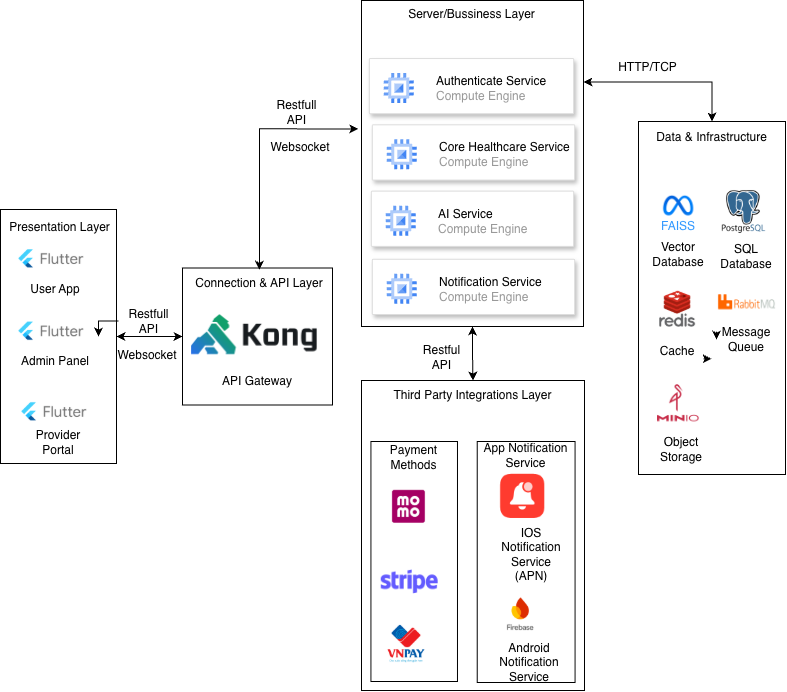
\includegraphics[width=1\textwidth]{Images/implement_arch.png}
    \vspace{10pt}
    
    % Thêm chú thích cho hình ảnh
    \caption{Kiến trúc hiện thực hệ thống}
    
    % Đặt nhãn để tham chiếu chéo (cross-reference)
    \label{fig:imple_arch}
\end{figure}

Hệ thống được thiết kế dựa trên mô hình Microservices hiện đại, chia thành 5 tầng chính với các công nghệ cụ thể như sau:

\subsection*{Tầng Giao Diện (Presentation Layer)}
Đây là tầng tương tác trực tiếp với người dùng cuối (tương ứng với Client Layer trong bản thiết kế trừu tượng).

\begin{itemize}
    \item \textbf{Công nghệ:} Flutter.
    \item \textbf{Mô tả:} Sử dụng Flutter làm công nghệ chủ đạo (Cross-platform) để xây dựng cả 3 ứng dụng client:
    \begin{itemize}
        \item \textit{User App:} Ứng dụng di động dành cho người dùng phổ thông.
        \item \textit{Admin Panel:} Trang quản trị hệ thống.
        \item \textit{Provider Portal:} Cổng thông tin dành cho các nhà cung cấp dịch vụ y tế/làm đẹp.
    \end{itemize}
    \item \textbf{Giao thức:} Các ứng dụng này giao tiếp với hệ thống backend thông qua RESTful API và WebSocket (dành cho các tính năng thời gian thực).
\end{itemize}

\subsection*{Tầng Kết Nối \& API (Connection \& API Layer)}
Đóng vai trò là cổng vào duy nhất (Entry point) cho mọi yêu cầu từ phía Client.

\begin{itemize}
    \item \textbf{Công nghệ:} Kong API Gateway.
    \item \textbf{Mô tả:} Thay thế cho khối "API Gateway" trừu tượng. Kong chịu trách nhiệm:
    \begin{itemize}
        \item Routing (định tuyến) request đến đúng microservice.
        \item Load balancing (cân bằng tải).
        \item Authentication/Authorization cơ bản (xác thực sơ bộ).
        \item Rate limiting (giới hạn băng thông) để bảo vệ hệ thống.
    \end{itemize}
\end{itemize}

\subsection*{Tầng Server \& Nghiệp Vụ (Server/Business Layer)}
Đây là lõi của hệ thống, được triển khai theo kiến trúc Microservices.

\begin{itemize}
    \item \textbf{Hạ tầng:} Compute Engine (Google Cloud Platform - GCP). Các dịch vụ được triển khai trên các máy ảo (VM) hoặc Container chạy trên VM.
    \item \textbf{Các dịch vụ thành phần:}
    \begin{itemize}
        \item \textit{Authenticate Service:} Xử lý đăng ký, đăng nhập, cấp phát token (JWT).
        \item \textit{Core Healthcare Service:} Xử lý nghiệp vụ chính như đặt lịch hẹn (Appointments), quản lý hồ sơ y tế, thanh toán.
        \item \textit{AI Service:} Chịu trách nhiệm về các tính năng thông minh (Chatbot, Recommendation System). Dịch vụ này giao tiếp chặt chẽ với Vector Database.
        \item \textit{Notification Service:} Quản lý việc gửi thông báo đẩy (Push) và Email.
    \end{itemize}
\end{itemize}

\subsection*{Tầng Dữ Liệu \& Hạ Tầng (Data \& Infrastructure Layer)}
Tầng này lưu trữ và quản lý luồng dữ liệu, cụ thể hóa các khối database trừu tượng:

\begin{itemize}
    \item \textbf{Relational Database (SQL):} Sử dụng \textbf{PostgreSQL}. Dùng để lưu trữ dữ liệu có cấu trúc (thông tin user, đơn hàng, lịch hẹn).
    \item \textbf{Vector Database:} Sử dụng \textbf{FAISS} (Facebook AI Similarity Search). Dùng để lưu trữ vector embeddings phục vụ cho AI Service (tìm kiếm ngữ nghĩa, gợi ý).
    \item \textbf{Cache:} Sử dụng \textbf{Redis}. Giúp tăng tốc độ truy xuất dữ liệu thường xuyên sử dụng và giảm tải cho Database chính.
    \item \textbf{Message Queue:} Sử dụng \textbf{RabbitMQ}. Đảm bảo giao tiếp bất đồng bộ (asynchronous) giữa các microservices (ví dụ: Core Service gửi sự kiện đến Notification Service mà không cần chờ đợi).
    \item \textbf{Object Storage:} Sử dụng \textbf{MinIO}. Giải pháp lưu trữ đối tượng (tương thích S3) dùng để lưu trữ file tĩnh, hình ảnh, tài liệu y tế (thay thế cho khối Cloud Storage trừu tượng).
\end{itemize}

\subsection*{Tầng Tích Hợp Bên Thứ Ba (Third-Party Integrations Layer)}
Kết nối với các dịch vụ bên ngoài để mở rộng tính năng.

\begin{itemize}
    \item \textbf{Cổng thanh toán (Payment Methods):} Tích hợp đa dạng bao gồm MoMo, Stripe (quốc tế), và VNPay (nội địa Việt Nam).
    \item \textbf{Dịch vụ thông báo (App Notification Service):}
    \begin{itemize}
        \item \textit{APNs (Apple Push Notification service):} Dành riêng cho thiết bị iOS.
        \item \textit{Firebase (FCM):} Dành cho Android và quản lý thông báo chung.
    \end{itemize}
\end{itemize}

\vspace{1cm} % Khoảng cách một chút trước phần nhận xét

\subsection*{Nhận xét tổng quan}
Kiến trúc này rất hiện đại và phù hợp với quy mô dự án nền tảng Health/Beauty. Việc tách biệt rõ ràng giữa PostgreSQL (nghiệp vụ) và FAISS (AI) cho thấy sự đầu tư kỹ lưỡng vào hiệu năng xử lý dữ liệu thông minh. Sử dụng MinIO cũng là một giải pháp hay để tự chủ (self-hosted) việc lưu trữ dữ liệu thay vì phụ thuộc hoàn toàn vào cloud public storage đắt đỏ.
\section{Phần Software – Triển khai ứng dụng}

Hệ thống Backend được xây dựng dựa trên \textbf{NestJS Framework}, tuân theo kiến trúc module hóa để đảm bảo tính mở rộng và bảo mật. Phần hiện thực được tổ chức theo bốn phân hệ chính dựa trên góc nhìn người dùng: (1)~Hạ tầng nền tảng dùng chung, (2)~Ứng dụng Người bệnh, (3)~Cổng Đối tác, và (4)~Trang Quản trị --- khớp với phân nhóm Use Case đã phân tích ở chương trước và kịch bản demo End-to-End trước Hội đồng.


% ===========================================================================
% 6.3.1  HẠ TẦNG NỀN TẢNG VÀ DỊCH VỤ CHUNG (CORE)
% ===========================================================================
\subsection{Hiện thực Hạ tầng nền tảng và Dịch vụ chung}

Trước khi đi vào chi tiết từng phân hệ người dùng, phần này trình bày các thành phần hạ tầng kỹ thuật dùng chung cho toàn bộ hệ thống. Đây là ``móng nhà'' mà cả ba cổng (User App, Partner Portal, Admin Portal) đều dựa trên: từ cơ chế xác thực JWT, chuẩn hóa dữ liệu DTO, quản lý tệp tin, đến hệ thống thông báo đa kênh và cầu nối với cụm AI microservices.

\subsubsection{Cấu hình và Khởi tạo hệ thống (Bootstrap \& Configuration)}

Điểm khởi chạy của ứng dụng nằm tại \texttt{src/main.ts}, nơi thiết lập các cấu hình toàn cục quan trọng cho bảo mật và tài liệu hóa API:

\begin{itemize}
    \item \textbf{Bảo mật HTTP:} Tích hợp thư viện \texttt{helmet} để thiết lập các HTTP headers an toàn và kích hoạt \texttt{enableCors()} cho phép các ứng dụng Client (Mobile/Web) truy cập tài nguyên.
    
    \item \textbf{Kiểm soát dữ liệu đầu vào:} Sử dụng \texttt{ValidationPipe} ở mức toàn cục (\texttt{globalPipes}) với tùy chọn \texttt{whitelist: true}. Điều này giúp tự động loại bỏ các trường dữ liệu thừa không được định nghĩa trong DTO.
    
    \item \textbf{Xác thực Webhook (Stripe):} Bật tùy chọn \texttt{rawBody: true} để xác thực chữ ký webhook Stripe. Khởi tạo \texttt{RedisIoAdapter} cho WebSocket scale ngang và kết nối RabbitMQ consumer với queue \texttt{checkout\_queue}.
\end{itemize}

\subsubsection{Module Thanh toán (Payment Gateway Module)}

\texttt{PaymentGatewayModule} hỗ trợ song parallel hai cổng thanh toán chính: MoMo (nội địa Việt Nam) và Stripe (quốc tế). Cấu trúc API như sau:

\begin{itemize}
    \item \textbf{Phía người dùng:} Các endpoint \texttt{POST /v1/user/payments/momo/*} và \texttt{POST /v1/user/payments/stripe/*} cho phép tạo đơn thanh toán, hoàn tiền, và kiểm tra trạng thái.
    
    \item \textbf{Phía callback:} Các endpoint công khai \texttt{POST /v1/public/momo/ipn} (Immediate Payment Notification) và \texttt{POST /v1/public/stripe/webhook} để xử lý các sự kiện từ phía gateway, theo mô hình server-to-server.
\end{itemize}

\subsubsection{Module Tích hợp AI (AI Service Integration)}

\texttt{AiServiceController} cung cấp endpoint nội bộ:

\begin{itemize}
    \item \texttt{POST /v1/ai/recommendations} - Trả về danh sách dịch vụ được gợi ý kèm thông tin đầy đủ (tên, mô tả, giá, hình ảnh, vị trí).
    
    \item Bảo vệ bằng API key header \texttt{X-AI-API-Key} để chỉ cho phép gọi machine-to-machine từ cụm AI Gateway.
\end{itemize}

\subsubsection{Cụm Microservices AI (FastAPI Services)}

Module \texttt{AuthModule} đóng vai trò trung tâm trong việc quản lý định danh, sử dụng kết hợp \textbf{Passport} và \textbf{JWT}.

\paragraph{Quy trình Đăng ký \& Đăng nhập}
\begin{itemize}
    \item \textbf{Đăng ký (\texttt{register}):} \texttt{AuthService} tiếp nhận DTO đăng ký, thực hiện băm mật khẩu (hashing) bằng thuật toán \texttt{bcrypt} trước khi lưu vào cơ sở dữ liệu. Nếu có thông tin \texttt{profile}, hệ thống sẽ khởi tạo đồng thời \texttt{Account} và \texttt{UserProfile} nhờ cơ chế \texttt{cascade: true} của TypeORM.
    
    \item \textbf{Đăng nhập (\texttt{login}):} Sử dụng \texttt{LocalStrategy} để xác thực email/password. Sau khi thành công, hệ thống cấp phát cặp token gồm \texttt{access\_token} (ngắn hạn) và \texttt{refresh\_token} (dài hạn).
\end{itemize}

\paragraph{Cơ chế Bảo mật Token (JWT Strategy)}
\begin{itemize}
    \item \textbf{Access Token:} Được ký (sign) bằng \texttt{jwtConstants.secret}. Các request đến API được bảo vệ bởi \texttt{JwtAuthGuard}, sử dụng \texttt{JwtStrategy} để trích xuất và xác thực token từ Header (\texttt{Bearer Token}).
    
    \item \textbf{Refresh Token Rotation \& Hashing:} Để tăng cường bảo mật, \texttt{refresh\_token} không được lưu trực tiếp dưới dạng plain-text. Hệ thống chỉ lưu bản băm (hash) của nó vào cột \texttt{refreshTokenHash} trong bảng \texttt{Account}. Khi user yêu cầu cấp mới token (\texttt{/auth/refresh}), hệ thống so sánh token gửi lên với hash trong DB. Điều này ngăn chặn việc sử dụng lại token cũ nếu bị lộ.
    
    \item \textbf{Logout an toàn:} API \texttt{/auth/logout} thực hiện xóa \texttt{refreshTokenHash} trong DB, đảm bảo token cũ mất hiệu lực ngay lập tức.
\end{itemize}

% TODO: Hình sơ đồ luồng JWT (login → sign → refresh rotation → hash DB → logout)

\subsubsection{Kiến trúc DTO và Validation}

Hệ thống áp dụng chặt chẽ mô hình \textbf{Data Transfer Object (DTO)} để kiểm soát dữ liệu giao tiếp:

\begin{itemize}
    \item \textbf{Validation Rules:} Sử dụng các decorator như \texttt{@IsEmail}, \texttt{@MinLength(8)} cho mật khẩu, và \texttt{@Matches} cho số điện thoại (Regex kiểm tra định dạng số Việt Nam \texttt{+84...}).
    
    \item \textbf{Nested Validation:} Hỗ trợ validate dữ liệu lồng nhau (ví dụ: object \texttt{profile} bên trong \texttt{register} request) thông qua \texttt{@ValidateNested} và \texttt{Type(() => RegisterProfileDto)}.
\end{itemize}

\subsubsection{Quản lý Tệp tin và Lưu trữ (S3 File Management)}

Module \texttt{S3Module} tích hợp với dịch vụ lưu trữ đối tượng tương thích S3 (MinIO) để quản lý tệp tin:

\begin{itemize}
    \item \textbf{Upload:} Tạo Pre-signed URL cho phép Client upload trực tiếp đến storage mà không qua Backend, giảm tải cho server.
    \item \textbf{Download:} Sinh Pre-signed URL có thời hạn để truy cập tệp tin (tài liệu doanh nghiệp, hình ảnh sản phẩm).
    \item \textbf{Quản lý tài liệu đối tác:} Thực thể \texttt{PartnerDocument} lưu metadata (loại tài liệu, URL, trạng thái) trong PostgreSQL, trong khi nội dung tệp thực tế nằm trên Object Storage.
\end{itemize}

\subsubsection{Hệ thống Thông báo đa kênh (Notification)}

Module \texttt{NotificationModule} cung cấp hệ thống thông báo đa kênh phục vụ cả ba portal, với ba controller phân quyền rõ ràng:

\begin{itemize}
    \item \textbf{WebSocket:} \texttt{NotificationGateway} đẩy thông báo tức thì (đặt lịch, tin nhắn mới, nhắc hẹn).
    \item \textbf{Push Notification (FCM):} \texttt{PushNotificationService} tích hợp Firebase Cloud Messaging qua thư viện \texttt{firebase-admin}. \texttt{UserDeviceController} quản lý đăng ký/hủy đăng ký device token.
    \item \textbf{Quản lý:} \texttt{UserNotificationController} (xem, đánh dấu đã đọc), \texttt{AdminNotificationController} (broadcast hệ thống).
    \item \textbf{Bất đồng bộ:} Sự kiện thông báo phát qua RabbitMQ từ các module nghiệp vụ (\texttt{BookingModule}, \texttt{ChatModule}), không làm chậm luồng xử lý chính.
\end{itemize}

% TODO: Hình kiến trúc Notification đa kênh (3 source → RabbitMQ → NotificationService → WS + FCM + DB)

\subsubsection{Module Tích hợp AI (\texttt{AiServiceModule})}

Cầu nối giữa Backend NestJS và cụm microservices AI (Python/FastAPI). Luồng hoạt động:

\begin{enumerate}
    \item AI Gateway gọi endpoint \texttt{/ai/recommendations} kèm danh sách \texttt{service\_id} cần làm giàu thông tin.
    \item \texttt{AiServiceService} truy vấn bảng \texttt{products} kèm quan hệ (category, media, employees) từ PostgreSQL.
    \item Kết quả ánh xạ thành \texttt{AiRecommendationsResponseDto} chứa đầy đủ thông tin (tên, mô tả, giá, hình ảnh, vị trí) để hiển thị trên ứng dụng.
\end{enumerate}

Endpoint bảo vệ bằng \texttt{AiApiKeyGuard}, chỉ service nội bộ được phép truy cập.

\subsubsection{Hạ tầng Liên kết và Cross-cutting Concerns}

\paragraph{Module RabbitMQ}

Cấu hình kết nối RabbitMQ cho giao tiếp bất đồng bộ giữa các module. Module đăng ký \texttt{ClientsModule} với giao thức AMQP, hỗ trợ TLS và virtual host riêng biệt. Sử dụng chính bởi \texttt{NotificationModule} (sự kiện thông báo) và \texttt{HealthServiceModule} (đồng bộ dữ liệu với AI Recommender).

\paragraph{Module Redis}

Cung cấp kết nối Redis cho toàn bộ ứng dụng qua \texttt{RedisService}:

\begin{itemize}
    \item \textbf{Caching:} Dữ liệu tra cứu thường xuyên (dịch vụ, banner).
    \item \textbf{Pub/Sub:} Phát sự kiện \texttt{service:created}, \texttt{service:updated}, \texttt{service:deleted} để AI Recommender đồng bộ vector store.
    \item \textbf{Distributed Locking:} Khóa phân tán cho slot đặt lịch, ngăn double-booking.
    \item \textbf{Session/TTL:} Checkout ticket, OTP, dữ liệu tạm thời.
\end{itemize}

% TODO: Hình sơ đồ Redis multi-purpose (4 blocks: Cache, Distributed Lock, Pub/Sub, Session/TTL)

\paragraph{Middleware, Interceptor và Guard}

Các cơ chế xuyên suốt (cross-cutting concerns):

\begin{itemize}
    \item \textbf{LoggingMiddleware:} Ghi method, URL, thời gian phản hồi, status code trên mọi route.
    \item \textbf{ResponseInterceptor:} Chuẩn hóa response về format \texttt{\{statusCode, message, data\}}.
    \item \textbf{PublicThrottlerGuard:} Rate limiting 100 request/60 giây cho route công khai.
    \item \textbf{WsContractBootstrapService:} Tự động đăng ký WebSocket event contracts khi khởi động.
\end{itemize}


% ===========================================================================
% 6.3.2  PHÂN HỆ ỨNG DỤNG NGƯỜI BỆNH (USER APP)
% ===========================================================================
\subsection{Hiện thực Phân hệ Ứng dụng Người bệnh (User App)}

Phân hệ này hiện thực toàn bộ trải nghiệm của người bệnh trên ứng dụng di động, từ lúc đăng ký tài khoản đến khi hoàn thành dịch vụ và đánh giá. Luồng trải nghiệm xuyên suốt bao gồm: tạo tài khoản và khảo sát sức khỏe $\rightarrow$ khám phá phòng khám/dịch vụ theo vị trí $\rightarrow$ tương tác với Chatbot AI $\rightarrow$ chọn dịch vụ vào giỏ hàng $\rightarrow$ đặt lịch với cơ chế khóa slot phân tán $\rightarrow$ thanh toán qua MoMo $\rightarrow$ đánh giá chuyên gia và dịch vụ.

\subsubsection{Đăng nhập và Đăng ký Tài khoản}

Luồng khởi tạo tài khoản của ứng dụng người bệnh được tổ chức theo mô hình tách riêng \textbf{đăng nhập} và \textbf{đăng ký}, giúp người dùng quay lại đăng nhập nhanh, đồng thời buộc người dùng mới hoàn thiện đủ thông tin định danh trước khi sử dụng các chức năng đặt lịch và thanh toán.

\begin{enumerate}
    \item \textbf{Màn hình vào cổng xác thực:} Người dùng chọn giữa hai nhánh thao tác chính là \texttt{Sign In} hoặc \texttt{Create an account}. Cách tổ chức này giảm nhầm lẫn giữa người dùng mới và người dùng đã có tài khoản.

    \item \textbf{Đăng nhập tài khoản hiện có:} Người dùng nhập email và mật khẩu, có thể sử dụng liên kết \texttt{Forgot Password?} khi quên mật khẩu. Giao diện đồng thời hỗ trợ đăng nhập nhanh bằng Google và Facebook cho các trường hợp không muốn dùng mật khẩu cục bộ.

    \item \textbf{Khởi tạo đăng ký bằng email:} Với người dùng mới, hệ thống yêu cầu nhập email trước, đồng thời hiển thị điều khoản sử dụng và chính sách riêng tư ngay ở bước đầu để ràng buộc sự đồng thuận trước khi tạo tài khoản.

    \item \textbf{Xác thực email bằng OTP:} Sau bước nhập email, người dùng nhập mã xác thực được gửi qua email để chứng minh quyền sở hữu địa chỉ đăng ký và giảm nguy cơ tạo tài khoản giả mạo.

    \item \textbf{Hoàn thiện hồ sơ đăng ký:} Sau khi xác thực OTP, người dùng tiếp tục nhập họ tên pháp lý, ngày sinh, mật khẩu, xác nhận mật khẩu và địa chỉ liên hệ. Đây là tập dữ liệu nền để tạo \texttt{Account} và \texttt{UserProfile} ban đầu.

    \item \textbf{Xác nhận và kích hoạt:} Khi người dùng nhấn \texttt{Agree \& Continue}, backend thực hiện kiểm tra hợp lệ dữ liệu, băm mật khẩu bằng \texttt{bcrypt}, lưu hồ sơ và cấp token truy cập để người dùng đi tiếp sang các bước cá nhân hóa tiếp theo.
\end{enumerate}

\begin{figure}[H]
\centering
\captionsetup[subfigure]{font=small,justification=centering}
\captionsetup{skip=6pt}
\begin{subfigure}[t]{0.48\linewidth}
    \centering
    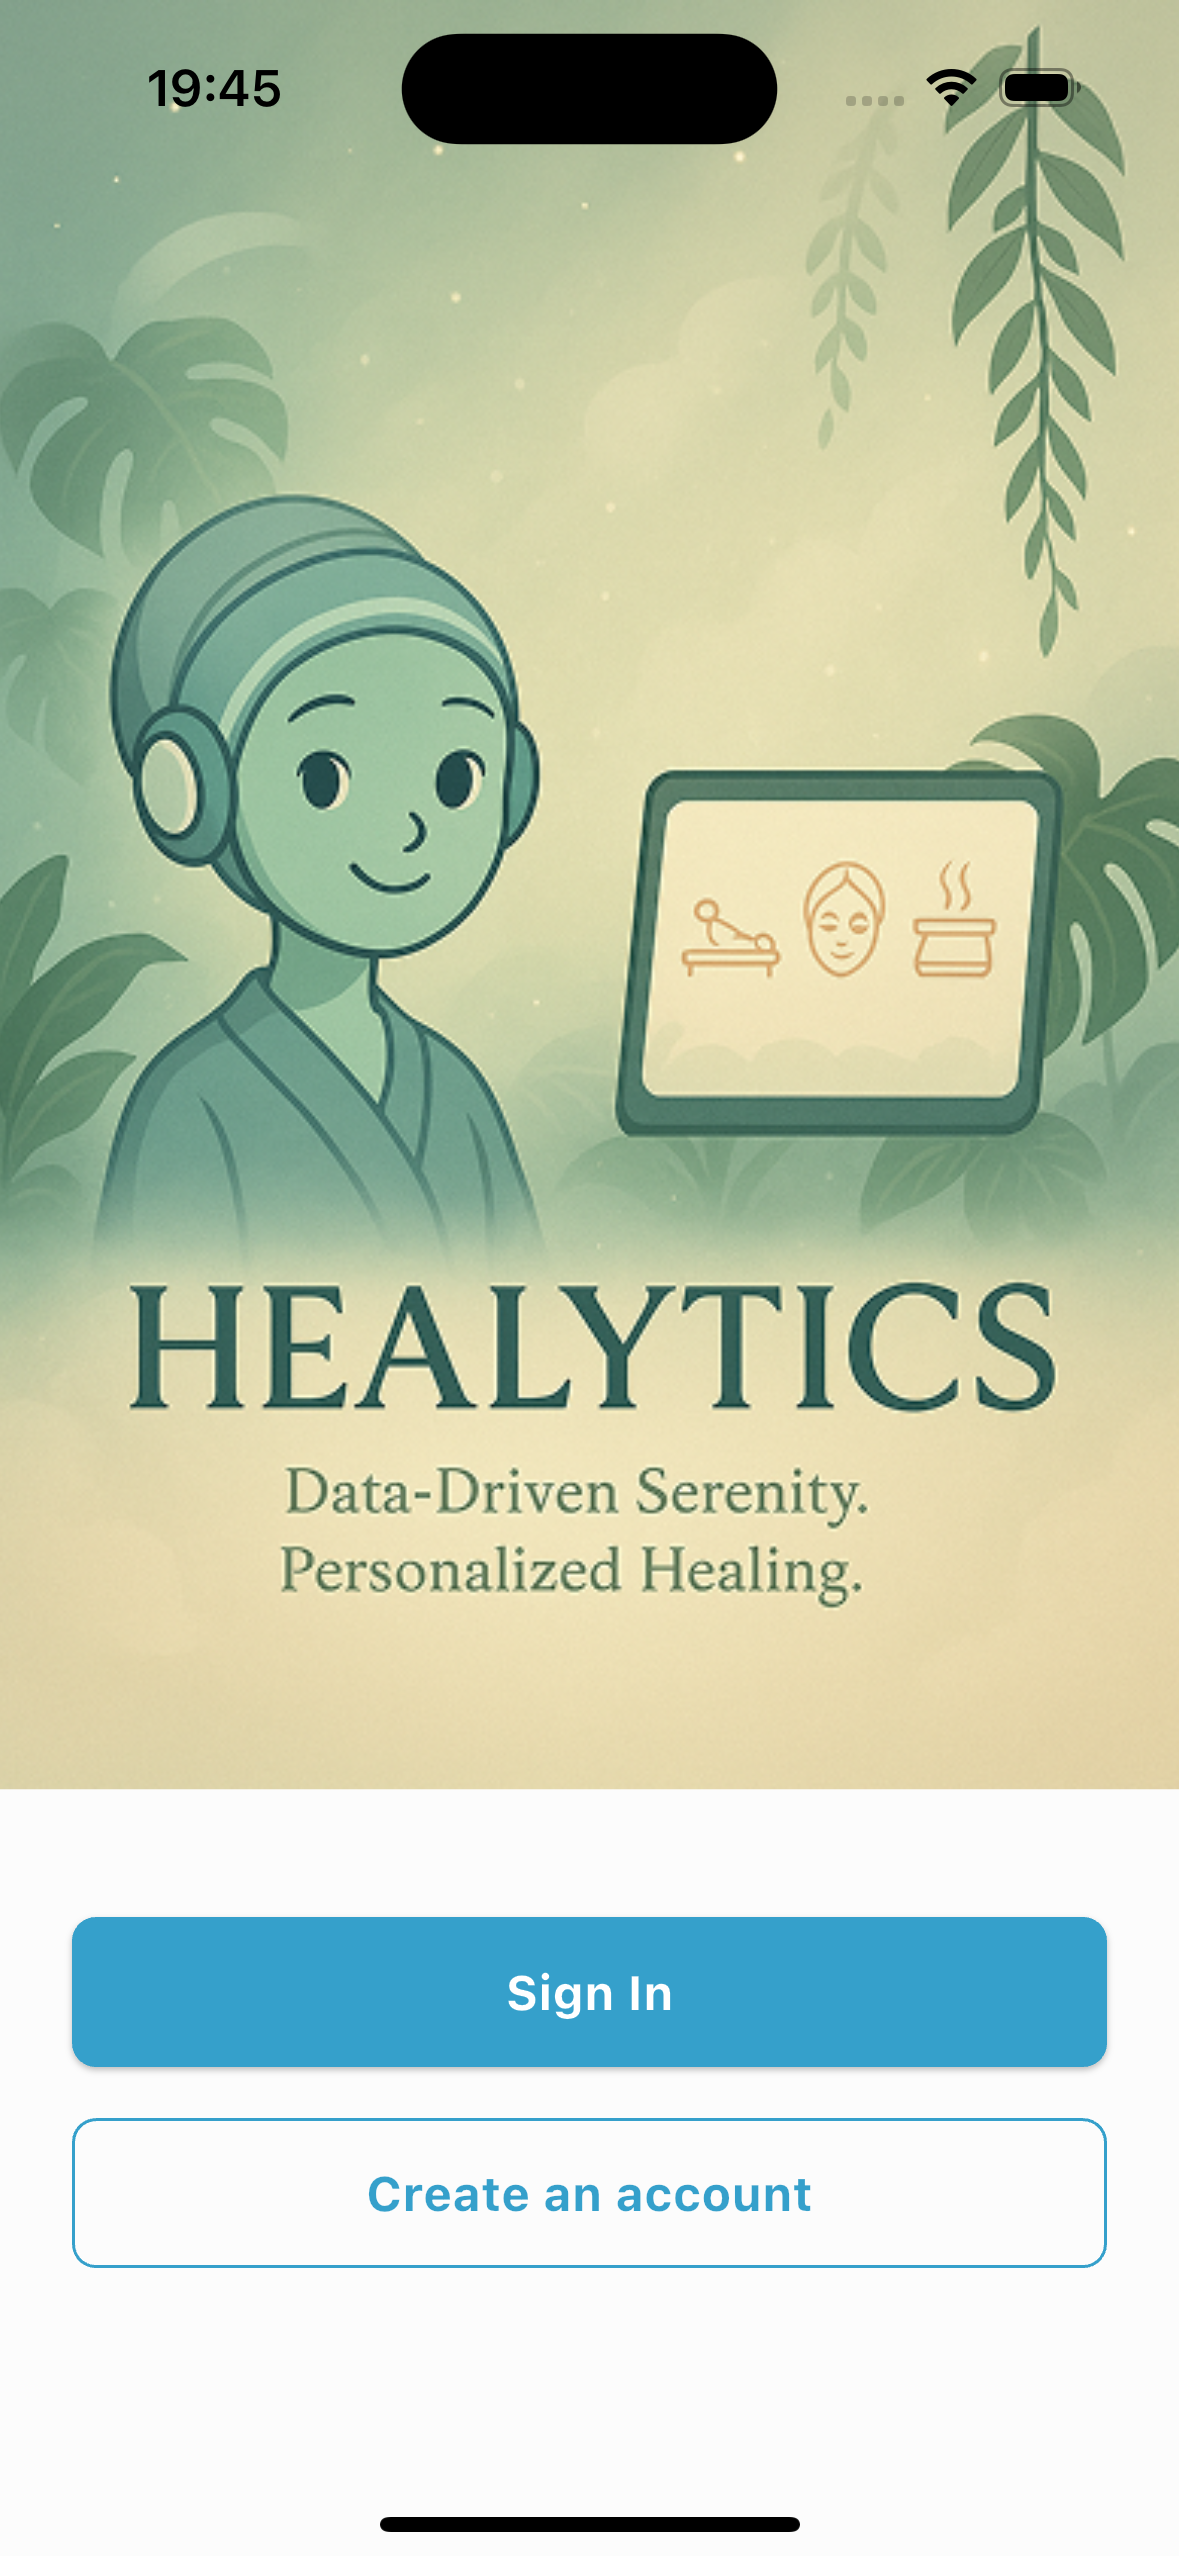
\includegraphics[width=\linewidth,height=0.4\textheight,keepaspectratio]{Images/Hiện thực/user_app/sign_in_sign_up/fig_user_auth_entry.png}
    \caption{Chọn \texttt{Sign In} hoặc \texttt{Create an account}}
    \label{fig:user_auth_entry}
\end{subfigure}
\hfill
\begin{subfigure}[t]{0.48\linewidth}
    \centering
    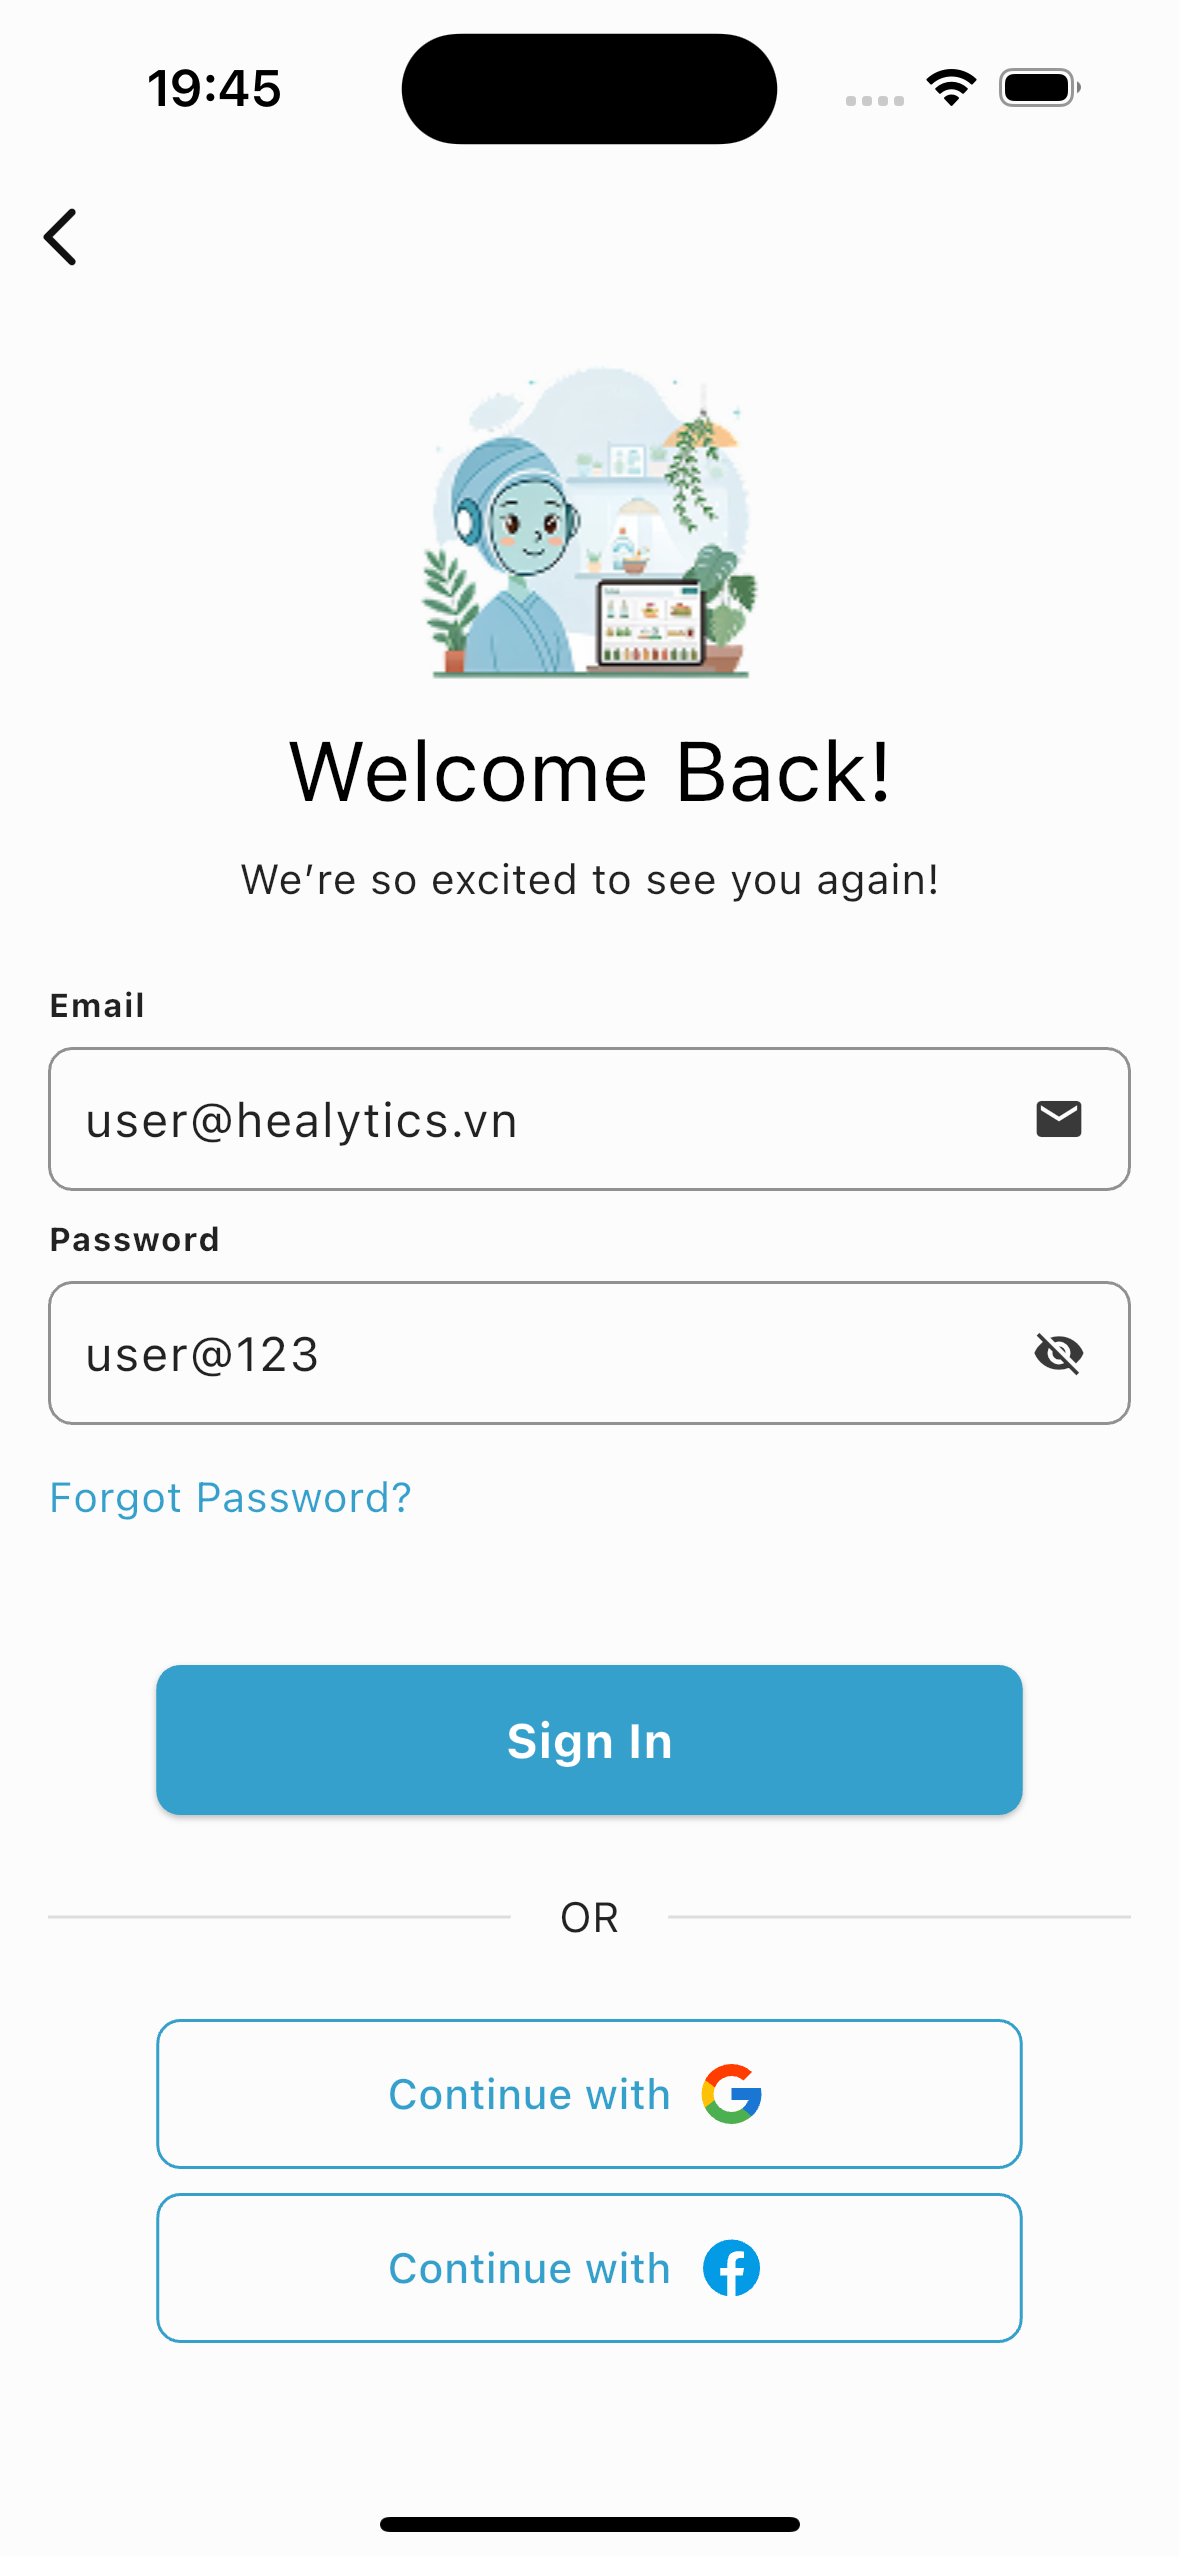
\includegraphics[width=\linewidth,height=0.4\textheight,keepaspectratio]{Images/Hiện thực/user_app/sign_in_sign_up/fig_user_auth_signin.png}
    \caption{Đăng nhập bằng email, mật khẩu hoặc social login}
    \label{fig:user_auth_signin}
\end{subfigure}
\par\medskip
\caption{Luồng Sign In của người dùng trên ứng dụng di động}
\label{fig:user_auth_signin_flow}
\end{figure}

\begin{figure}[H]
\centering
\captionsetup[subfigure]{font=small,justification=centering}
\captionsetup{skip=8pt}
\begin{subfigure}[t]{0.48\linewidth}
    \centering
    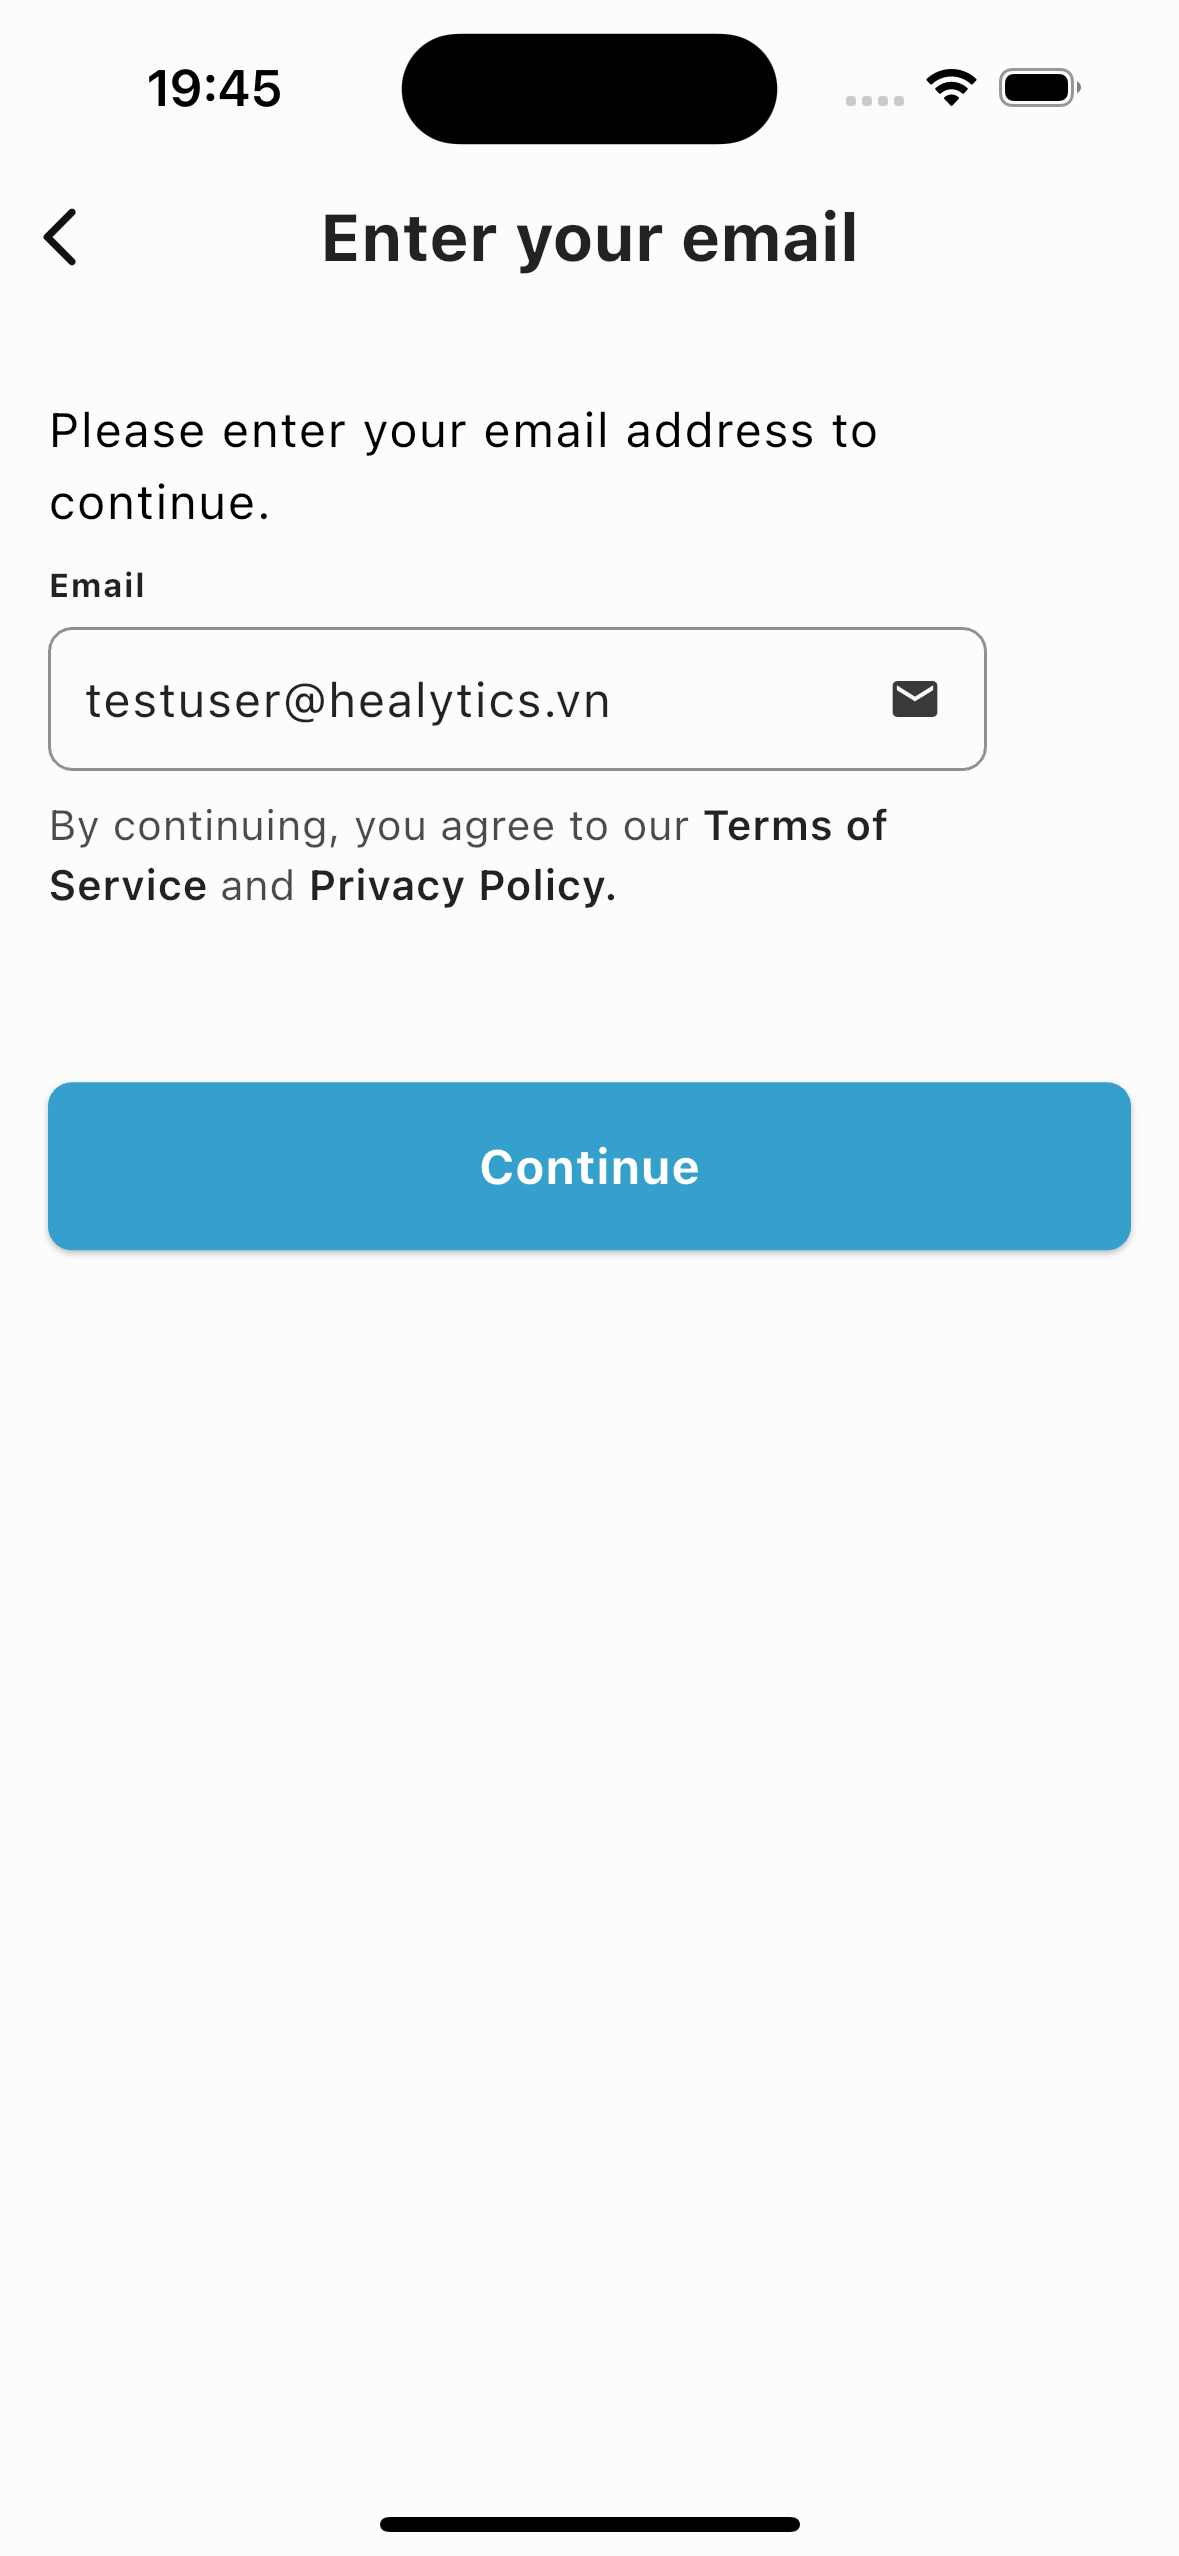
\includegraphics[width=\linewidth,height=0.4\textheight,keepaspectratio]{Images/Hiện thực/user_app/sign_in_sign_up/fig_user_auth_email.png}
    \caption{Nhập email đăng ký}
    \label{fig:user_auth_email}
\end{subfigure}
\hfill
\begin{subfigure}[t]{0.48\linewidth}
    \centering
    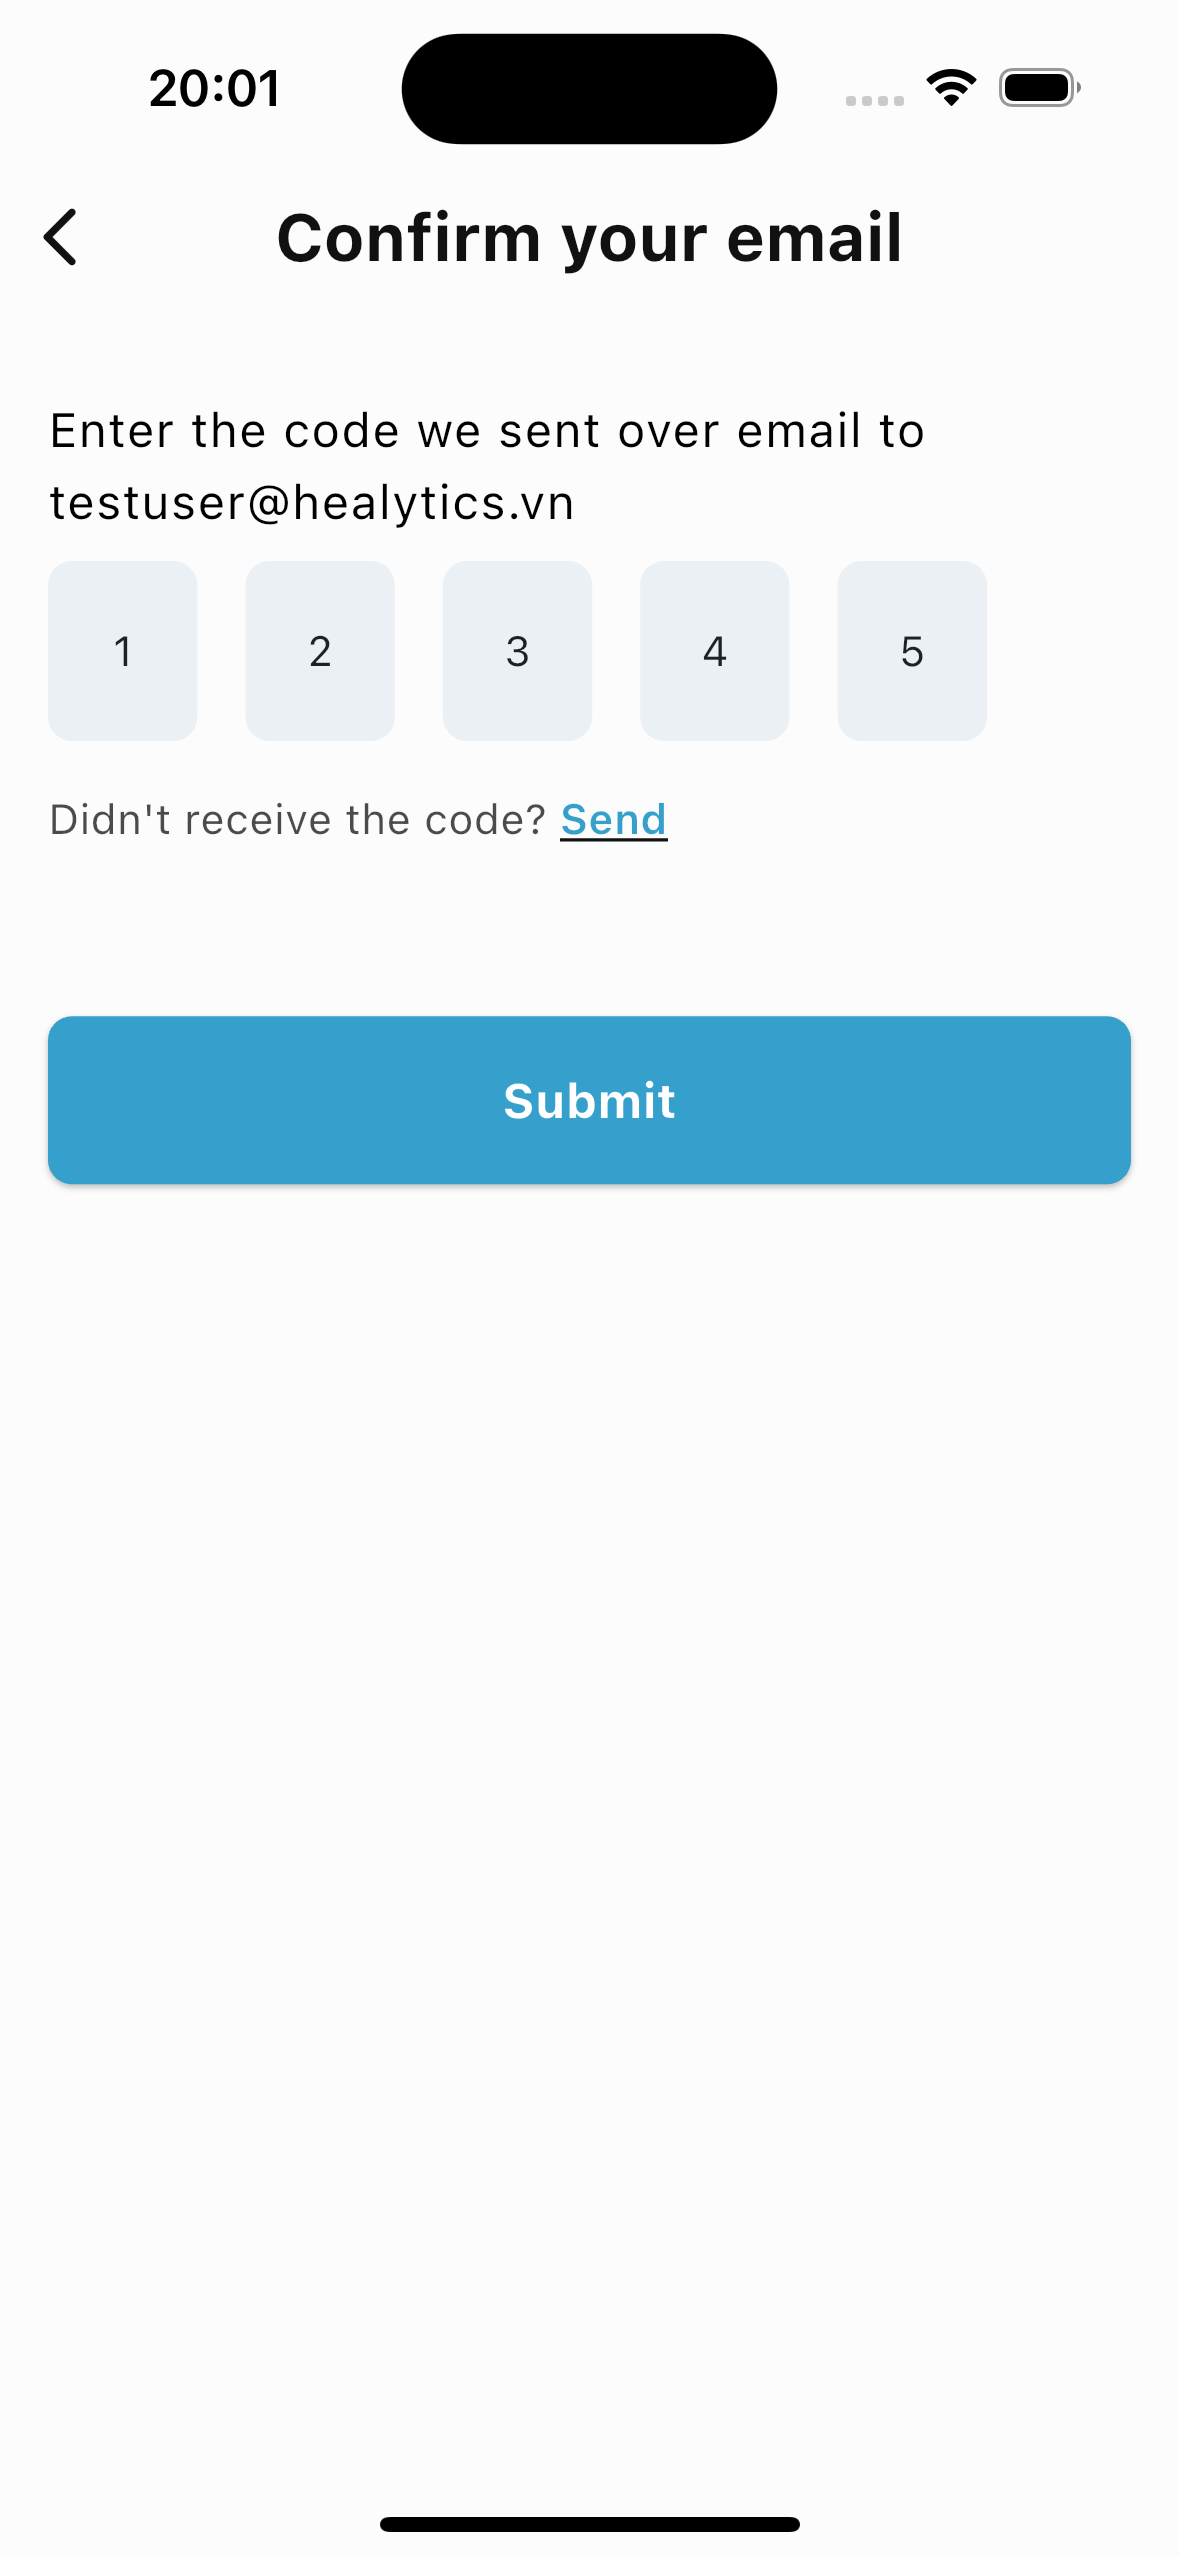
\includegraphics[width=\linewidth,height=0.4\textheight,keepaspectratio]{Images/Hiện thực/user_app/sign_in_sign_up/fig_user_auth_otp.png}
    \caption{Xác thực email bằng mã OTP}
    \label{fig:user_auth_otp}
\end{subfigure}
\par\medskip
\begin{subfigure}[t]{0.48\linewidth}
    \centering
    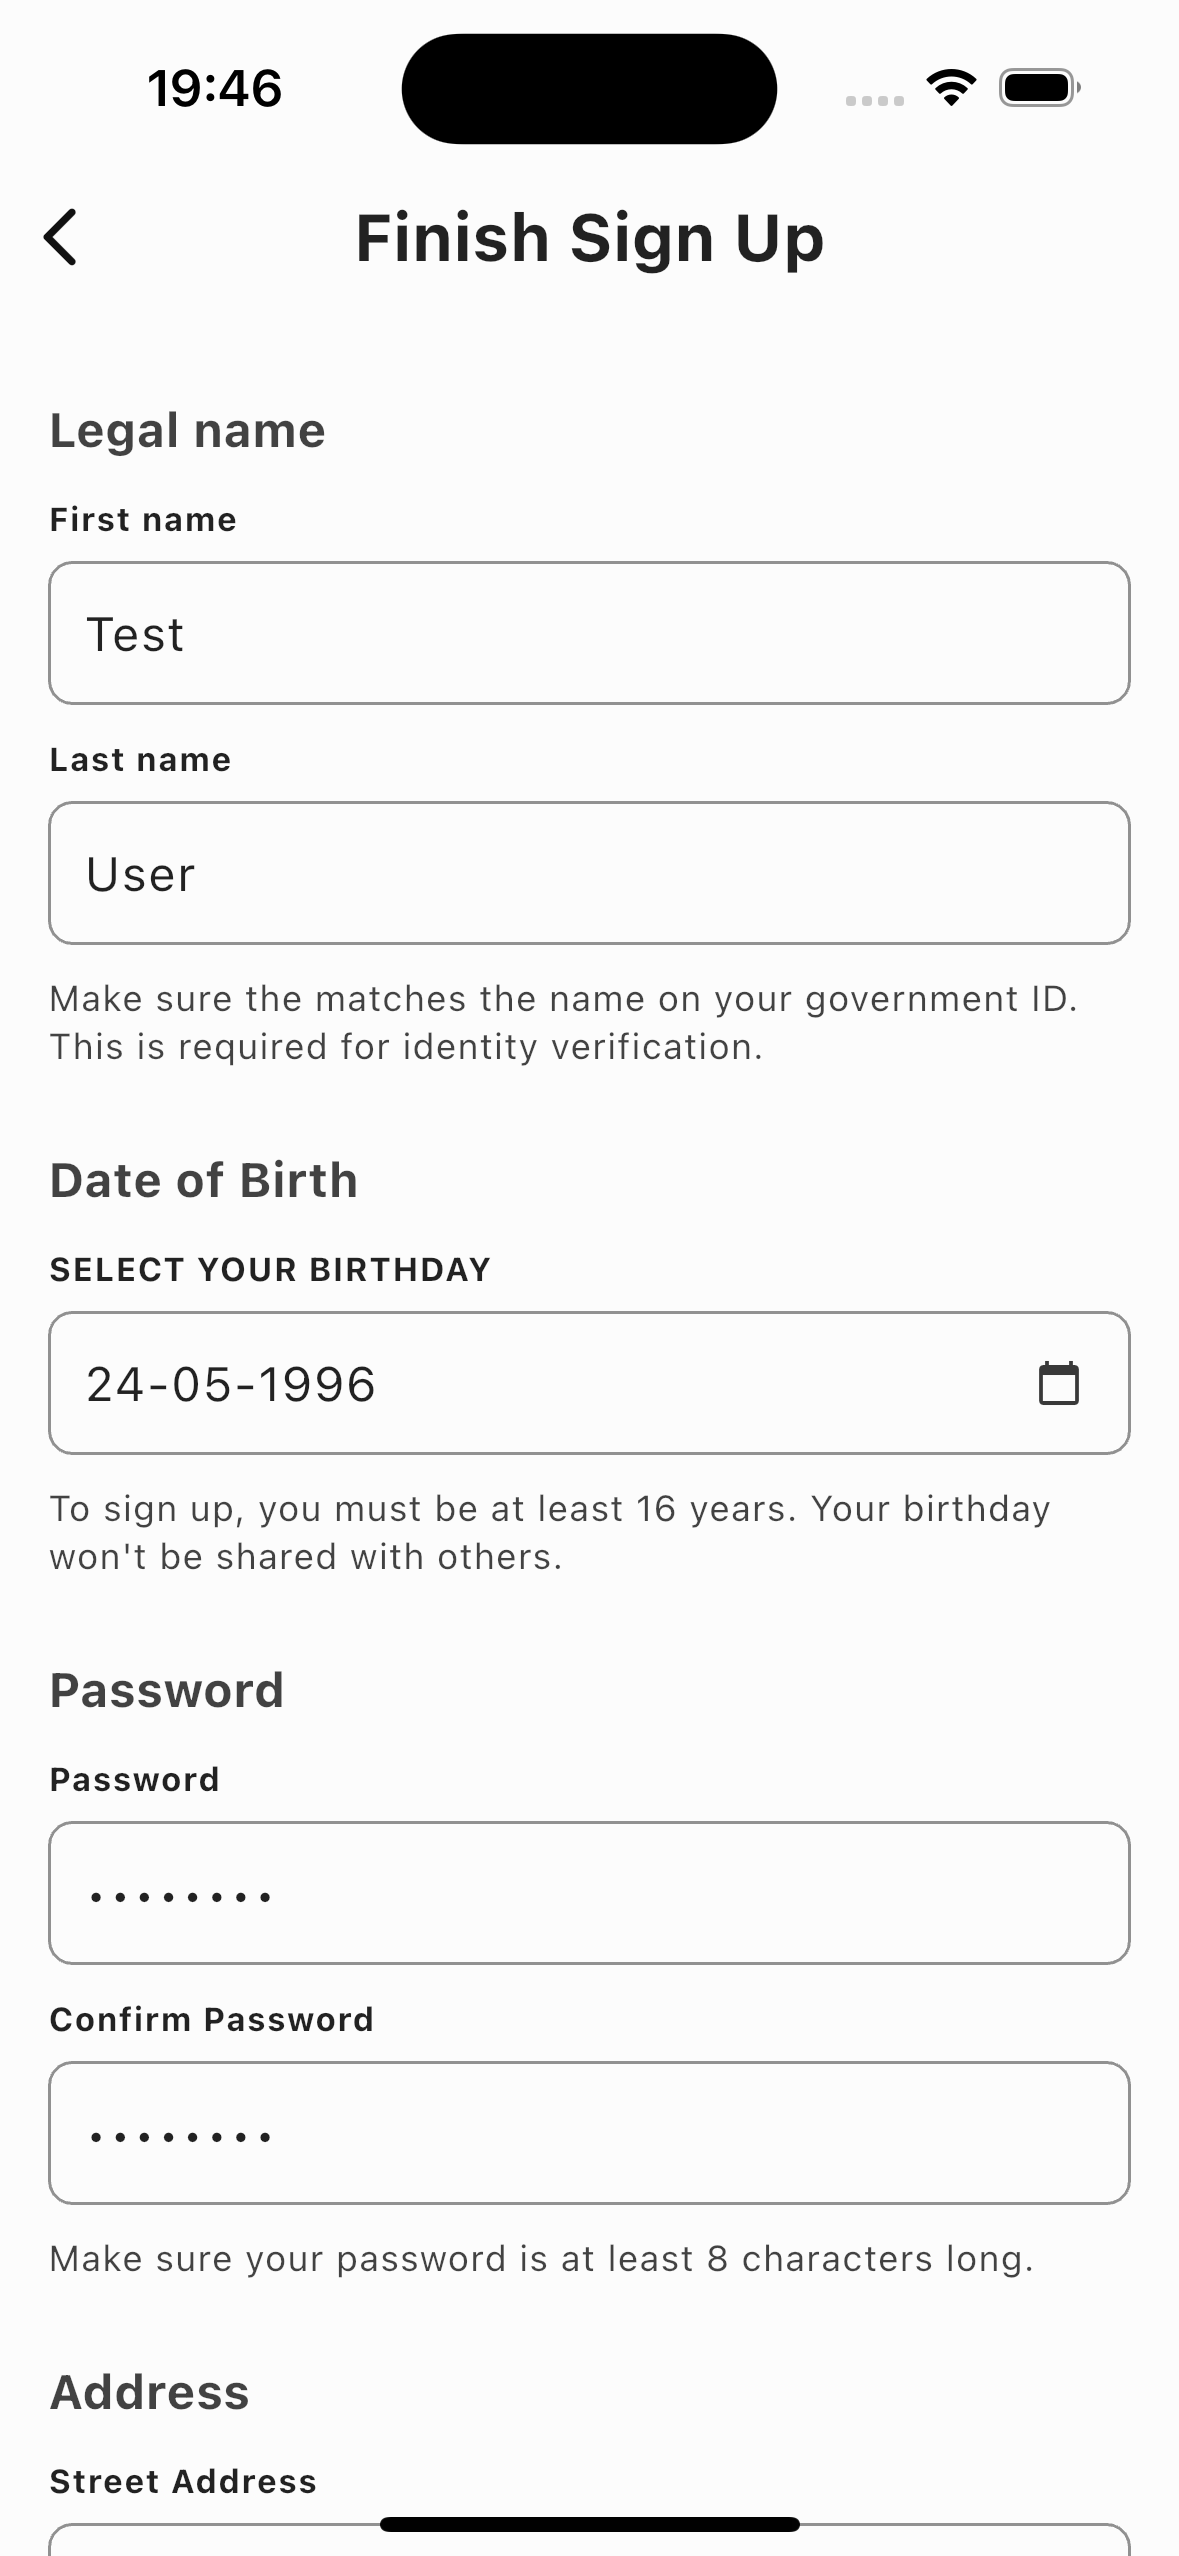
\includegraphics[width=\linewidth,height=0.4\textheight,keepaspectratio]{Images/Hiện thực/user_app/sign_in_sign_up/fig_user_auth_signup_profile.png}
    \caption{Điền thông tin cá nhân và ngày sinh}
    \label{fig:user_auth_signup_profile}
\end{subfigure}
\hfill
\begin{subfigure}[t]{0.48\linewidth}
    \centering
    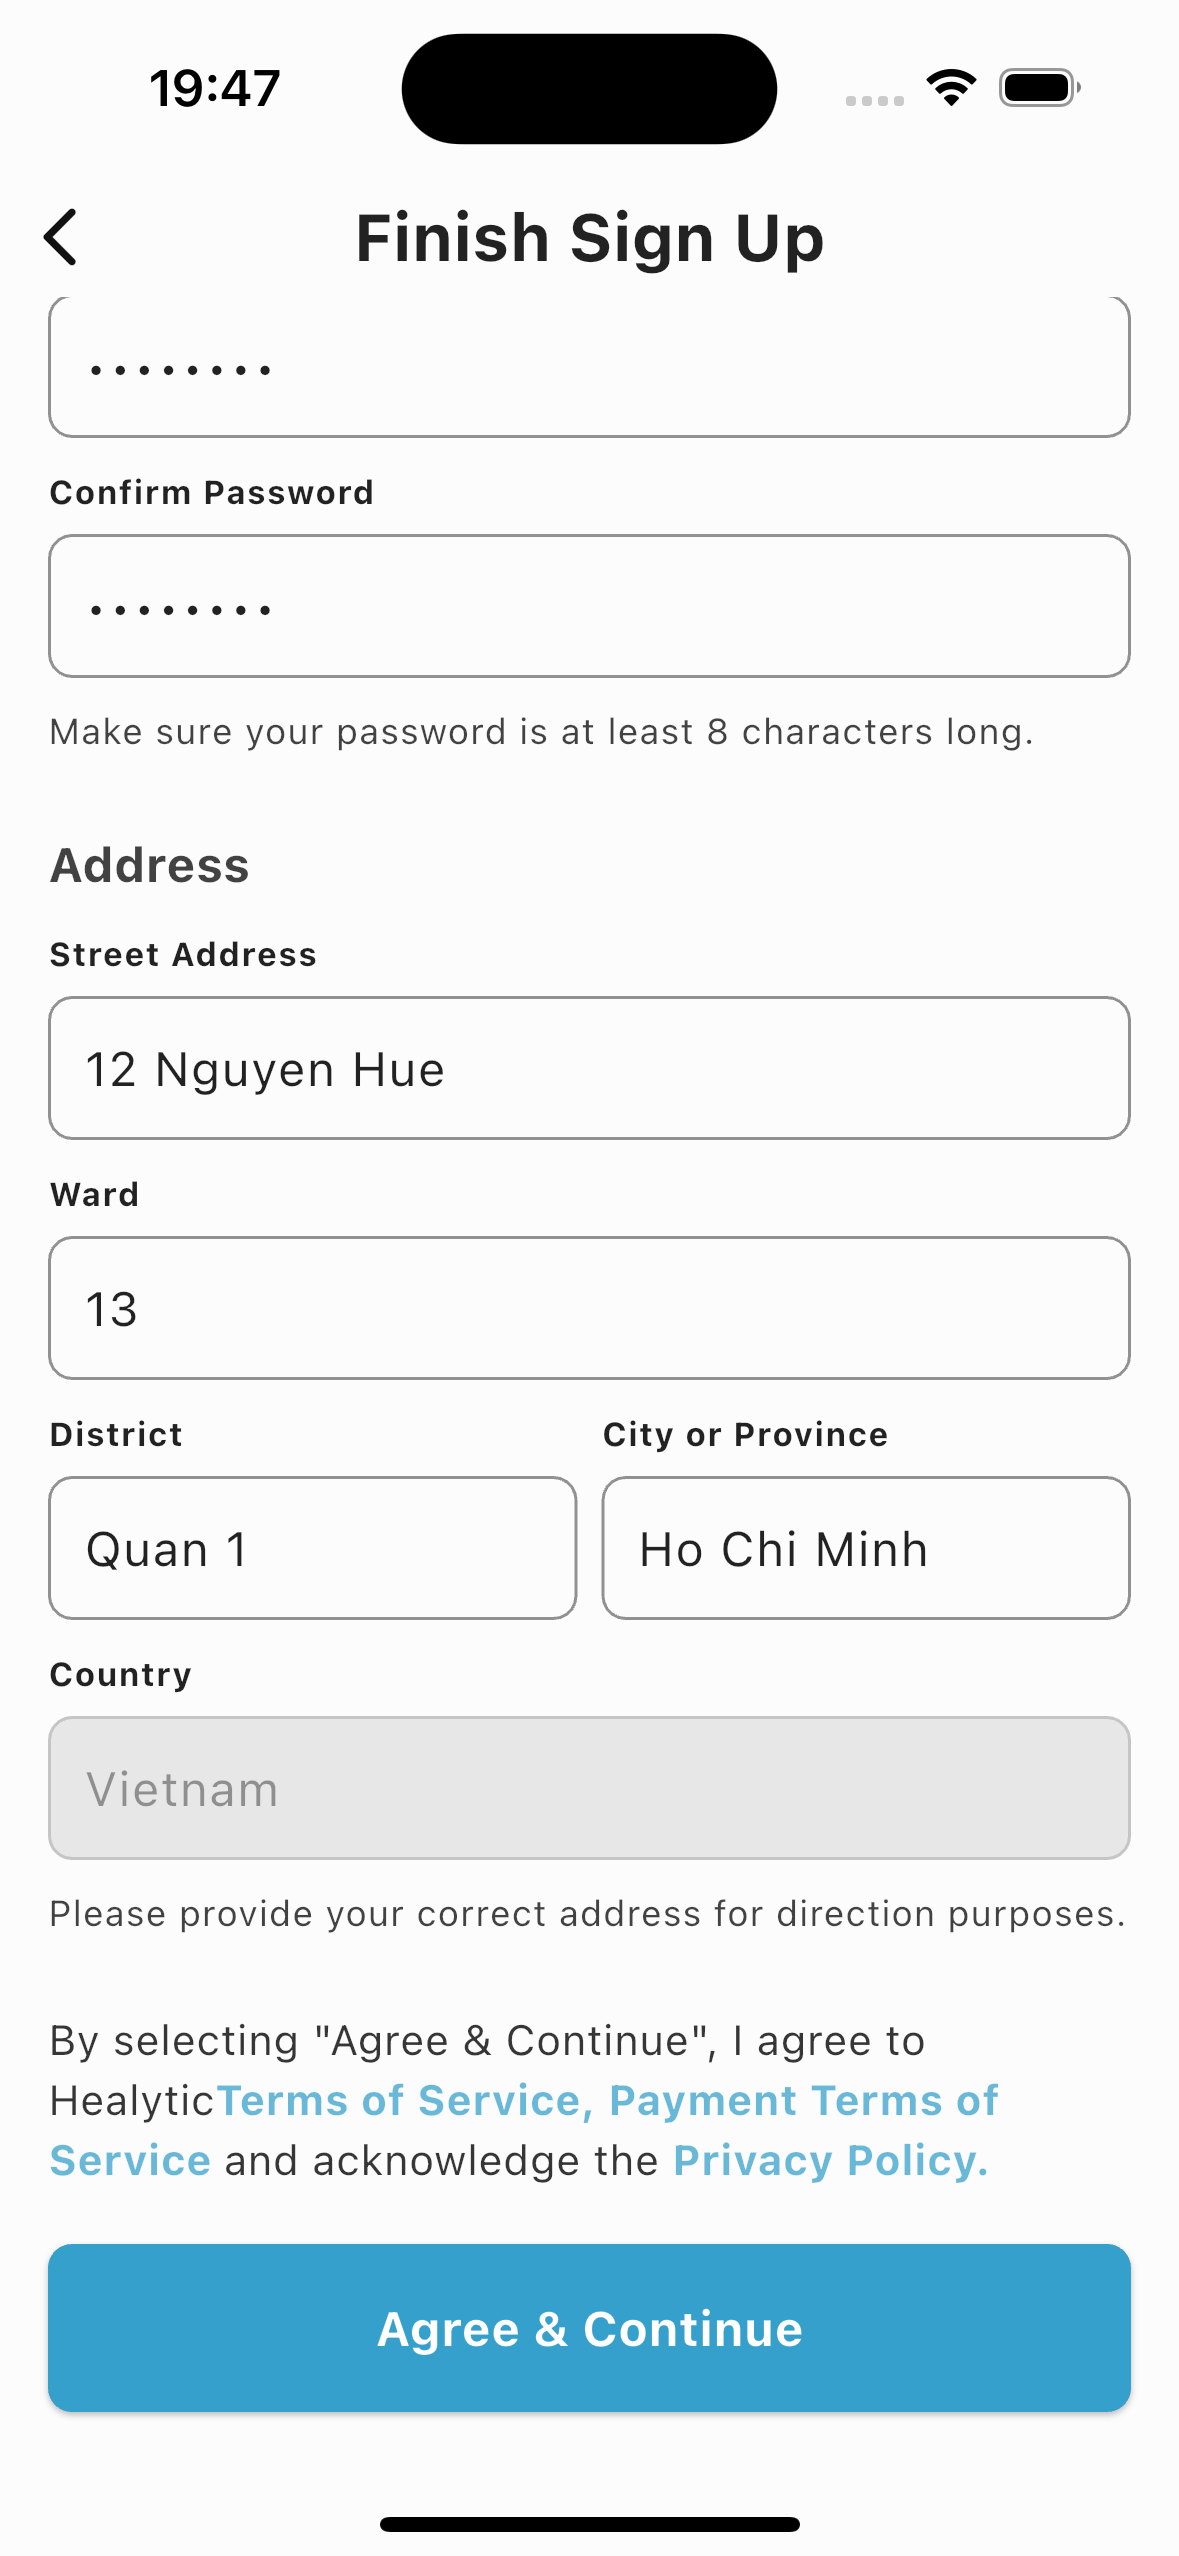
\includegraphics[width=\linewidth,height=0.4\textheight,keepaspectratio]{Images/Hiện thực/user_app/sign_in_sign_up/fig_user_auth_signup_address.png}
    \caption{Địa chỉ, điều khoản và xác nhận đăng ký}
    \label{fig:user_auth_signup_address}
\end{subfigure}
\par\medskip
\caption{Luồng Sign Up của người dùng trên ứng dụng di động}
\label{fig:user_auth_signup_flow}
\end{figure}

\paragraph{Mô tả dữ liệu và ràng buộc giao diện}

\begin{itemize}
    \item \textbf{Email:} Là định danh đăng nhập chính, được thu thập ngay từ đầu để kiểm tra định dạng và tránh trùng lặp tài khoản.
    \item \textbf{Mật khẩu:} Giao diện yêu cầu tối thiểu 8 ký tự và có trường \texttt{Confirm Password} để giảm lỗi nhập sai trước khi gửi request lên server.
    \item \textbf{Ngày sinh:} Hệ thống hiển thị ràng buộc độ tuổi tối thiểu 16 tuổi, phù hợp với yêu cầu sử dụng dịch vụ và xác minh danh tính cơ bản.
    \item \textbf{Họ tên pháp lý và địa chỉ:} Bao gồm tên thật, địa chỉ đường, phường/xã, quận/huyện, tỉnh/thành và quốc gia; đây là nhóm dữ liệu cần thiết cho nhận diện hồ sơ người dùng và các tác vụ điều hướng, đặt lịch, thanh toán.
    \item \textbf{Điều khoản sử dụng:} Trước khi hoàn tất đăng ký, người dùng phải đồng ý với \texttt{Terms of Service}, \texttt{Payment Terms of Service} và \texttt{Privacy Policy}, tạo cơ sở pháp lý cho toàn bộ giao dịch phát sinh sau đó.
\end{itemize}

\subsubsection{Khám phá Dịch vụ và Phòng khám}

\paragraph{Module Dịch vụ Sức khỏe (\texttt{HealthServiceModule})}

Module nghiệp vụ cốt lõi phía người dùng, quản lý vòng đời dịch vụ sức khỏe trên nền tảng. \texttt{UserHealthServiceController} cung cấp các endpoint:

\begin{itemize}
    \item \textbf{Tìm kiếm dịch vụ:} Hỗ trợ tìm theo từ khóa, lọc theo danh mục (\texttt{categoryId}), tags, khoảng giá (\texttt{minPrice}/\texttt{maxPrice}), và khoảng cách địa lý.
    \item \textbf{Phân trang và sắp xếp:} Hỗ trợ sort theo giá, đánh giá trung bình, lượt đặt, hoặc khoảng cách từ vị trí người dùng.
    \item \textbf{Chi tiết dịch vụ:} Trả về đầy đủ thông tin bao gồm \texttt{ProductDefinition} (thời lượng), \texttt{ProductMedia} (hình ảnh), \texttt{ProductEmployeeEligibility} (chuyên gia đủ điều kiện), và \texttt{ProductFeatureTag} (tags đặc trưng).
\end{itemize}

Mỗi dịch vụ (\texttt{Product}) liên kết với các thực thể con: \texttt{ProductMedia} (hình ảnh/video), \texttt{ProductFacilityImage} (ảnh cơ sở), \texttt{ProductTag}/\texttt{ProductFeatureTag} (tags), \texttt{ProductEmployeeEligibility} (chuyên gia đủ điều kiện), \texttt{ProductResourceRequirement} (yêu cầu thiết bị), và \texttt{DocumentRequirement} (giấy tờ cần từ phía bệnh nhân).

% \begin{figure}[H]
%     \centering
%     \begin{subfigure}[t]{0.3\textwidth}
%         \centering
%         
\includegraphics[width=\linewidth]{Images/Hiện thực/fig_user_home.png}
%         \caption{Trang chủ với banner và danh mục}
%     \end{subfigure}
%     \hfill
%     \begin{subfigure}[t]{0.3\textwidth}
%         \centering
%         \includegraphics[width=\linewidth]{Images/Hiện thực/fig_user_explore.png}
%         \caption{Khám phá dịch vụ theo vị trí}
%     \end{subfigure}
%     \hfill
%     \begin{subfigure}[t]{0.3\textwidth}
%         \centering
%         
\includegraphics[width=\linewidth]{Images/Hiện thực/fig_user_service_detail.png}
%         \caption{Chi tiết dịch vụ}
%     \end{subfigure}
%     \caption{Luồng khám phá dịch vụ và phòng khám trên ứng dụng di động}
%     \label{fig:user_explore_flow}
% \end{figure}

\paragraph{Module Phòng khám (\texttt{ClinicModule})}

Module cung cấp trang thông tin chi tiết phòng khám cho người dùng thông qua \texttt{UserClinicController}, tổ chức theo 3 tab:

\begin{itemize}
    \item \textbf{\texttt{GET /clinics/:id/info} --- Tab ``Cửa hàng'':} Thông tin tổng quan phòng khám gồm: tên, ảnh bìa, logo, gallery, chỉ số tin cậy (rating trung bình, số đánh giá, kinh nghiệm, số khách hàng), danh sách chứng chỉ (\texttt{PartnerCertification}), và top 5 chuyên gia (kèm kinh nghiệm tính từ \texttt{start\_date} hoặc \texttt{experience\_years}).

    \item \textbf{\texttt{GET /clinics/:id/products} --- Tab ``Dịch vụ'':} Danh mục dịch vụ có phân trang, lọc theo danh mục, sắp xếp (popular, latest, top\_sales, price\_asc, price\_desc), và tìm kiếm theo tên. Mỗi dịch vụ hiển thị giá gốc, giá khuyến mãi, thời lượng, và số lượt đặt.

    \item \textbf{\texttt{GET /clinics/:id/reviews} --- Tab ``Đánh giá'':} Đánh giá phân trang, lọc theo số sao (\texttt{starCount}) hoặc chỉ hiển thị đánh giá có ảnh (\texttt{hasMedia}).
\end{itemize}

\begin{figure}[H]
\centering
\captionsetup[subfigure]{font=small,justification=centering}
\captionsetup{skip=6pt}
\begin{subfigure}[t]{0.48\linewidth}
    \centering
    
\includegraphics[width=\linewidth,height=0.38\textheight,keepaspectratio]{Images/Hiện thực/user_app/clinic_info/fig_clinic_info_1.png}
    \caption{Tab Cửa hàng -- phần tổng quan}
    \label{fig:clinic_info_overview}
\end{subfigure}
\hfill
\begin{subfigure}[t]{0.48\linewidth}
    \centering
    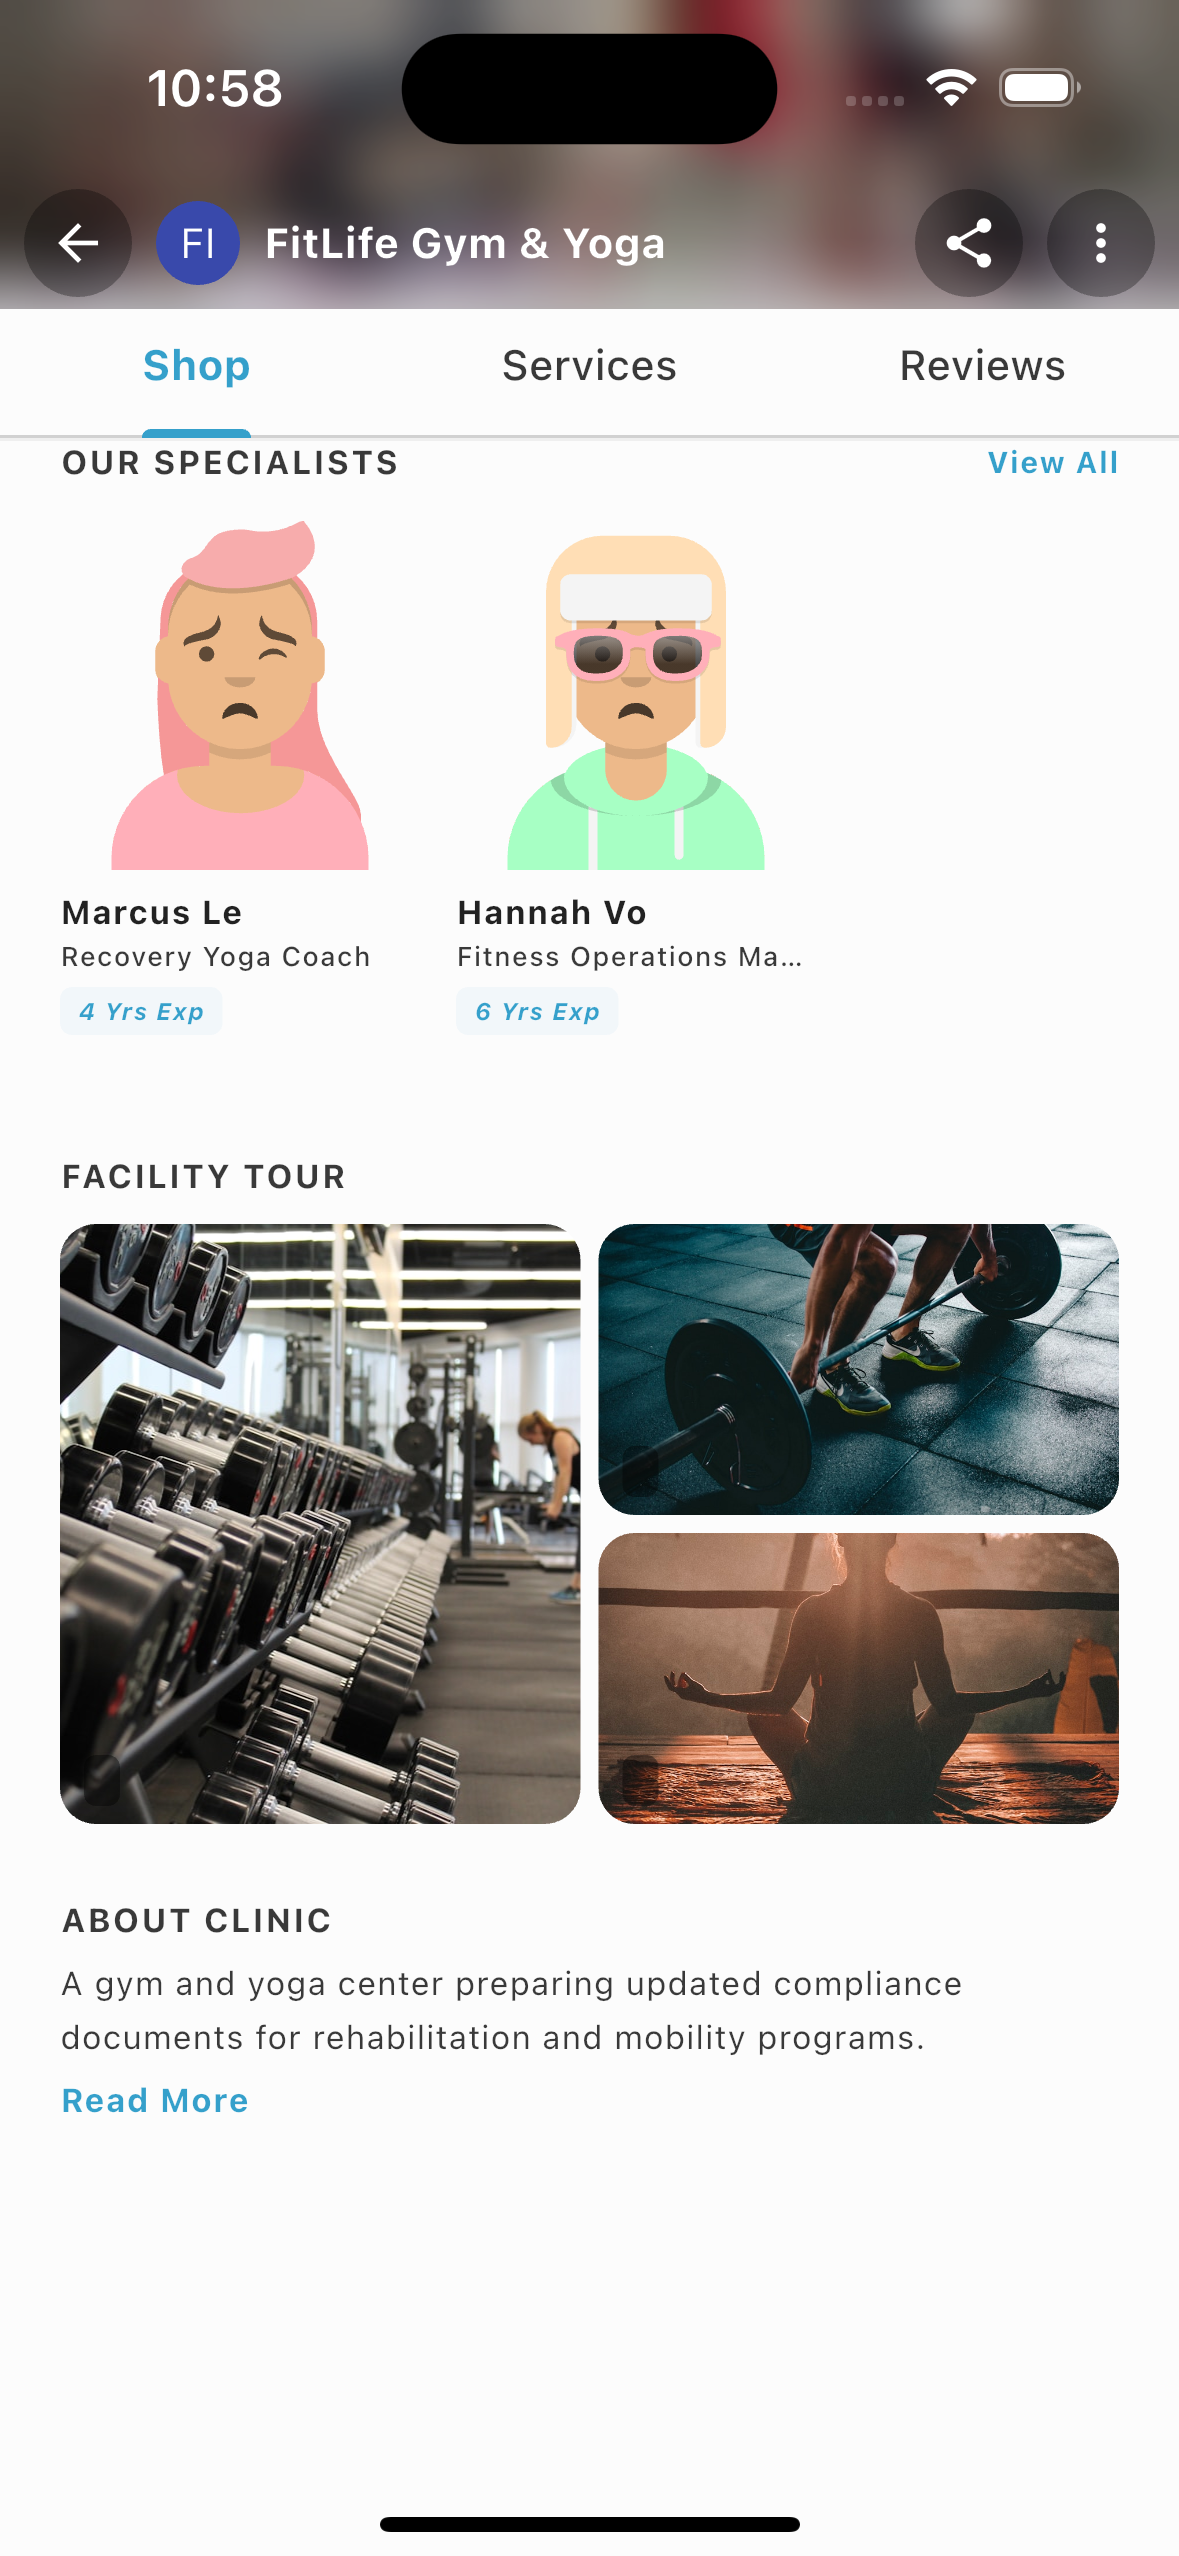
\includegraphics[width=\linewidth,height=0.38\textheight,keepaspectratio]{Images/Hiện thực/user_app/clinic_info/fig_clinic_info_2.png}
    \caption{Tab Cửa hàng -- cơ sở vật chất}
    \label{fig:clinic_info_facility}
\end{subfigure}
\par\medskip
\begin{subfigure}[t]{0.48\linewidth}
    \centering
    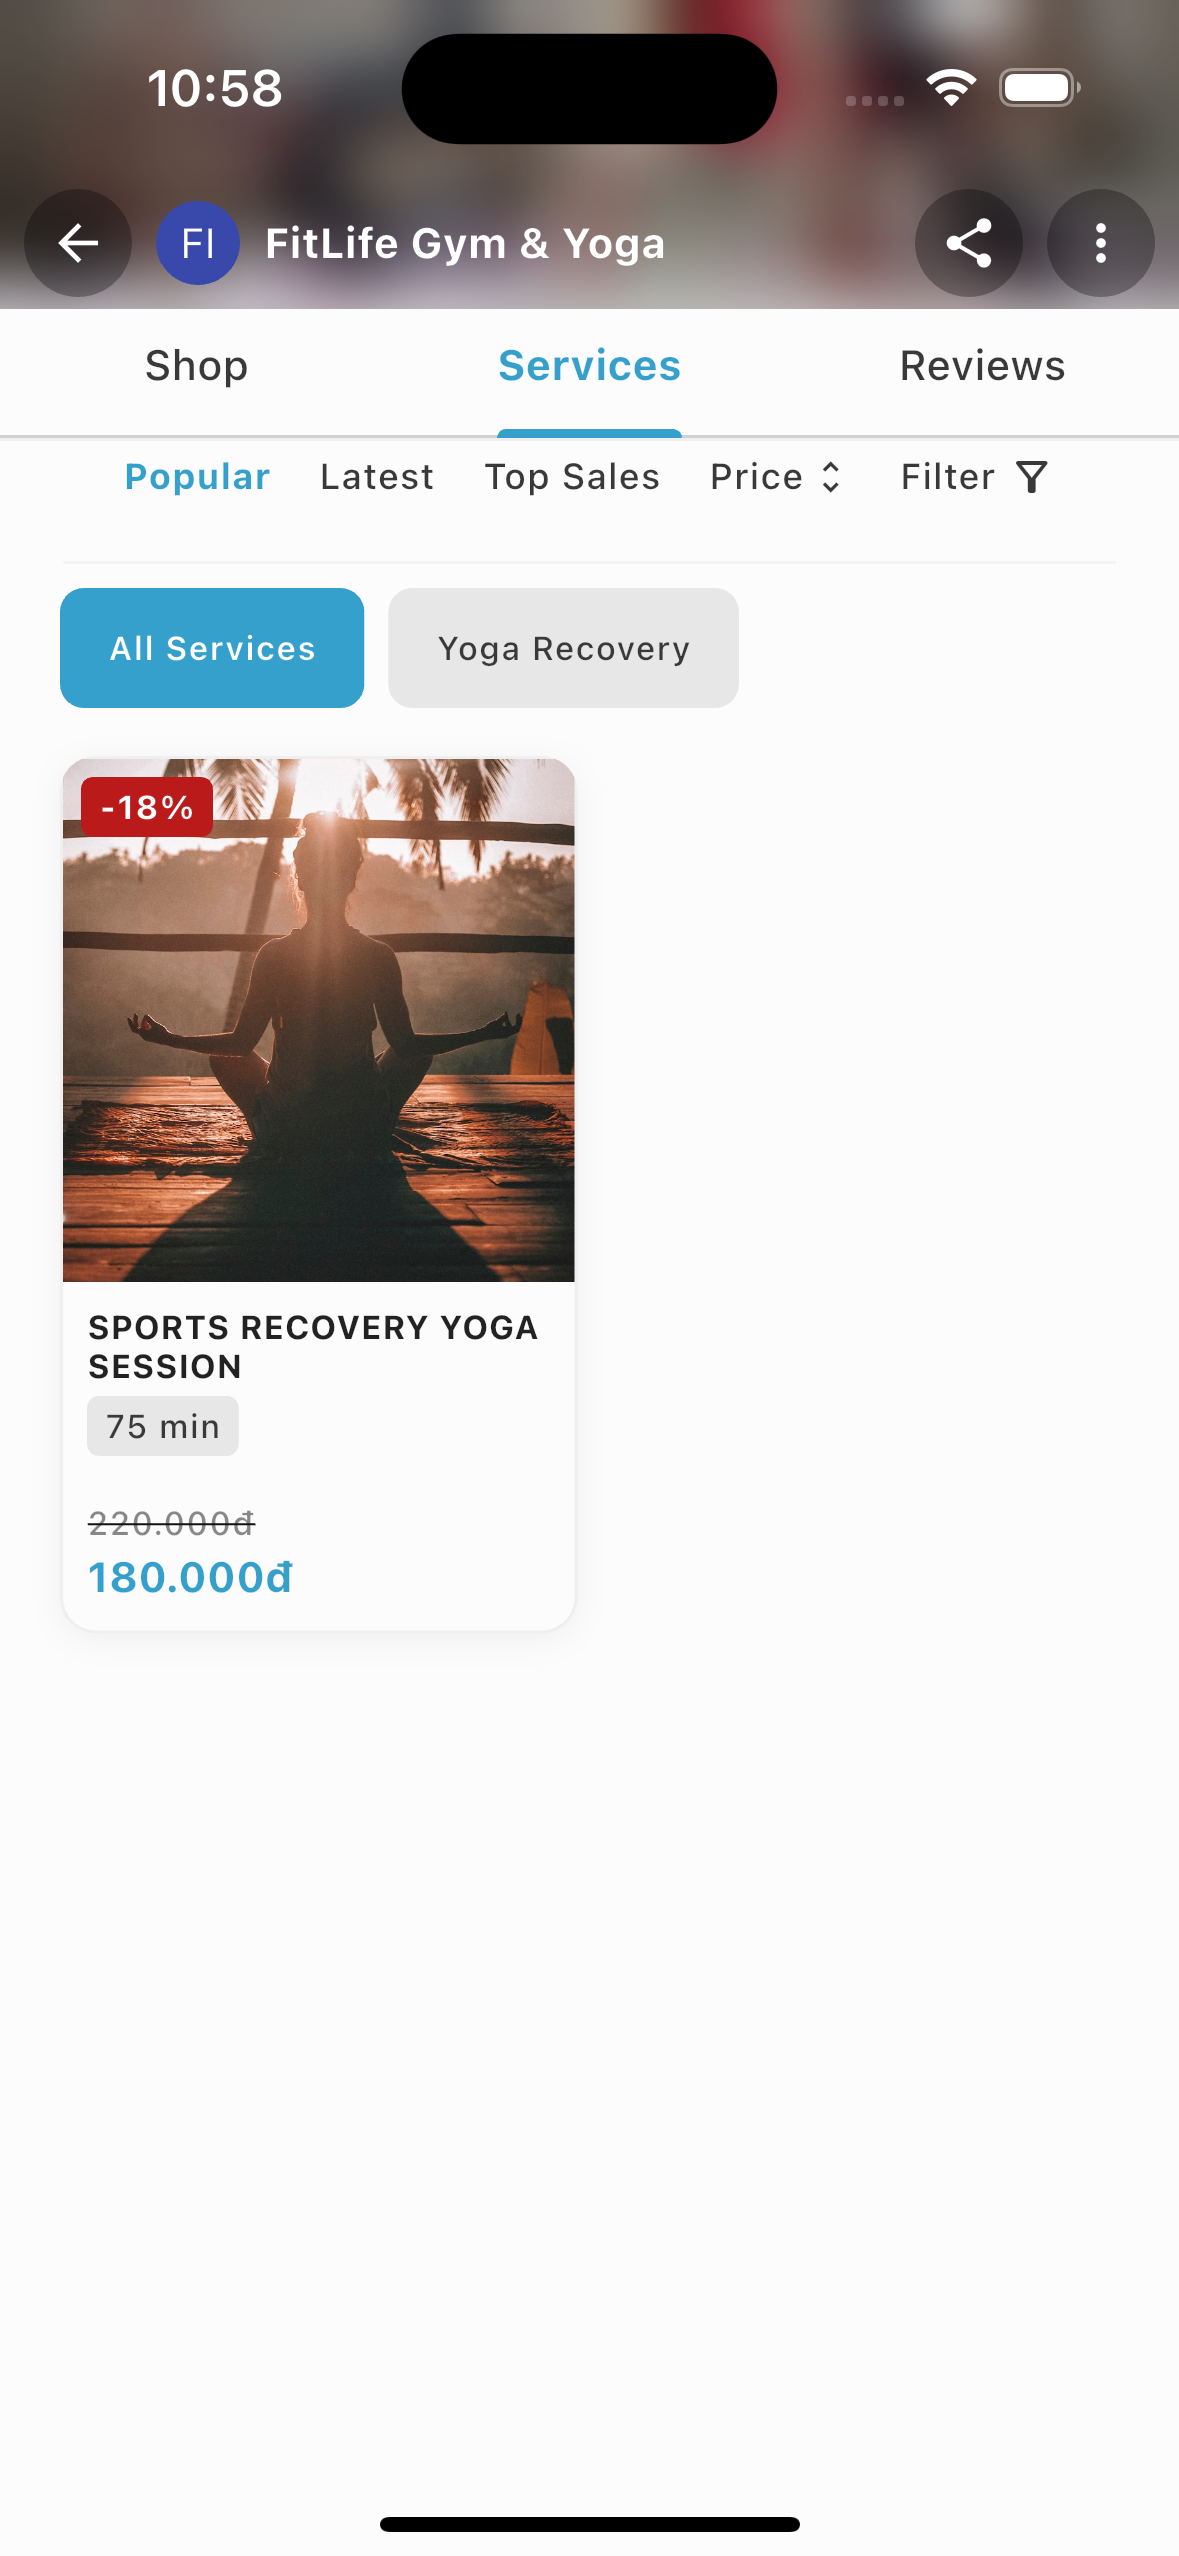
\includegraphics[width=\linewidth,height=0.38\textheight,keepaspectratio]{Images/Hiện thực/user_app/clinic_info/fig_clinic_info_3.png}
    \caption{Tab Dịch vụ -- danh sách dịch vụ}
    \label{fig:clinic_info_services}
\end{subfigure}
\hfill
\begin{subfigure}[t]{0.48\linewidth}
    \centering
    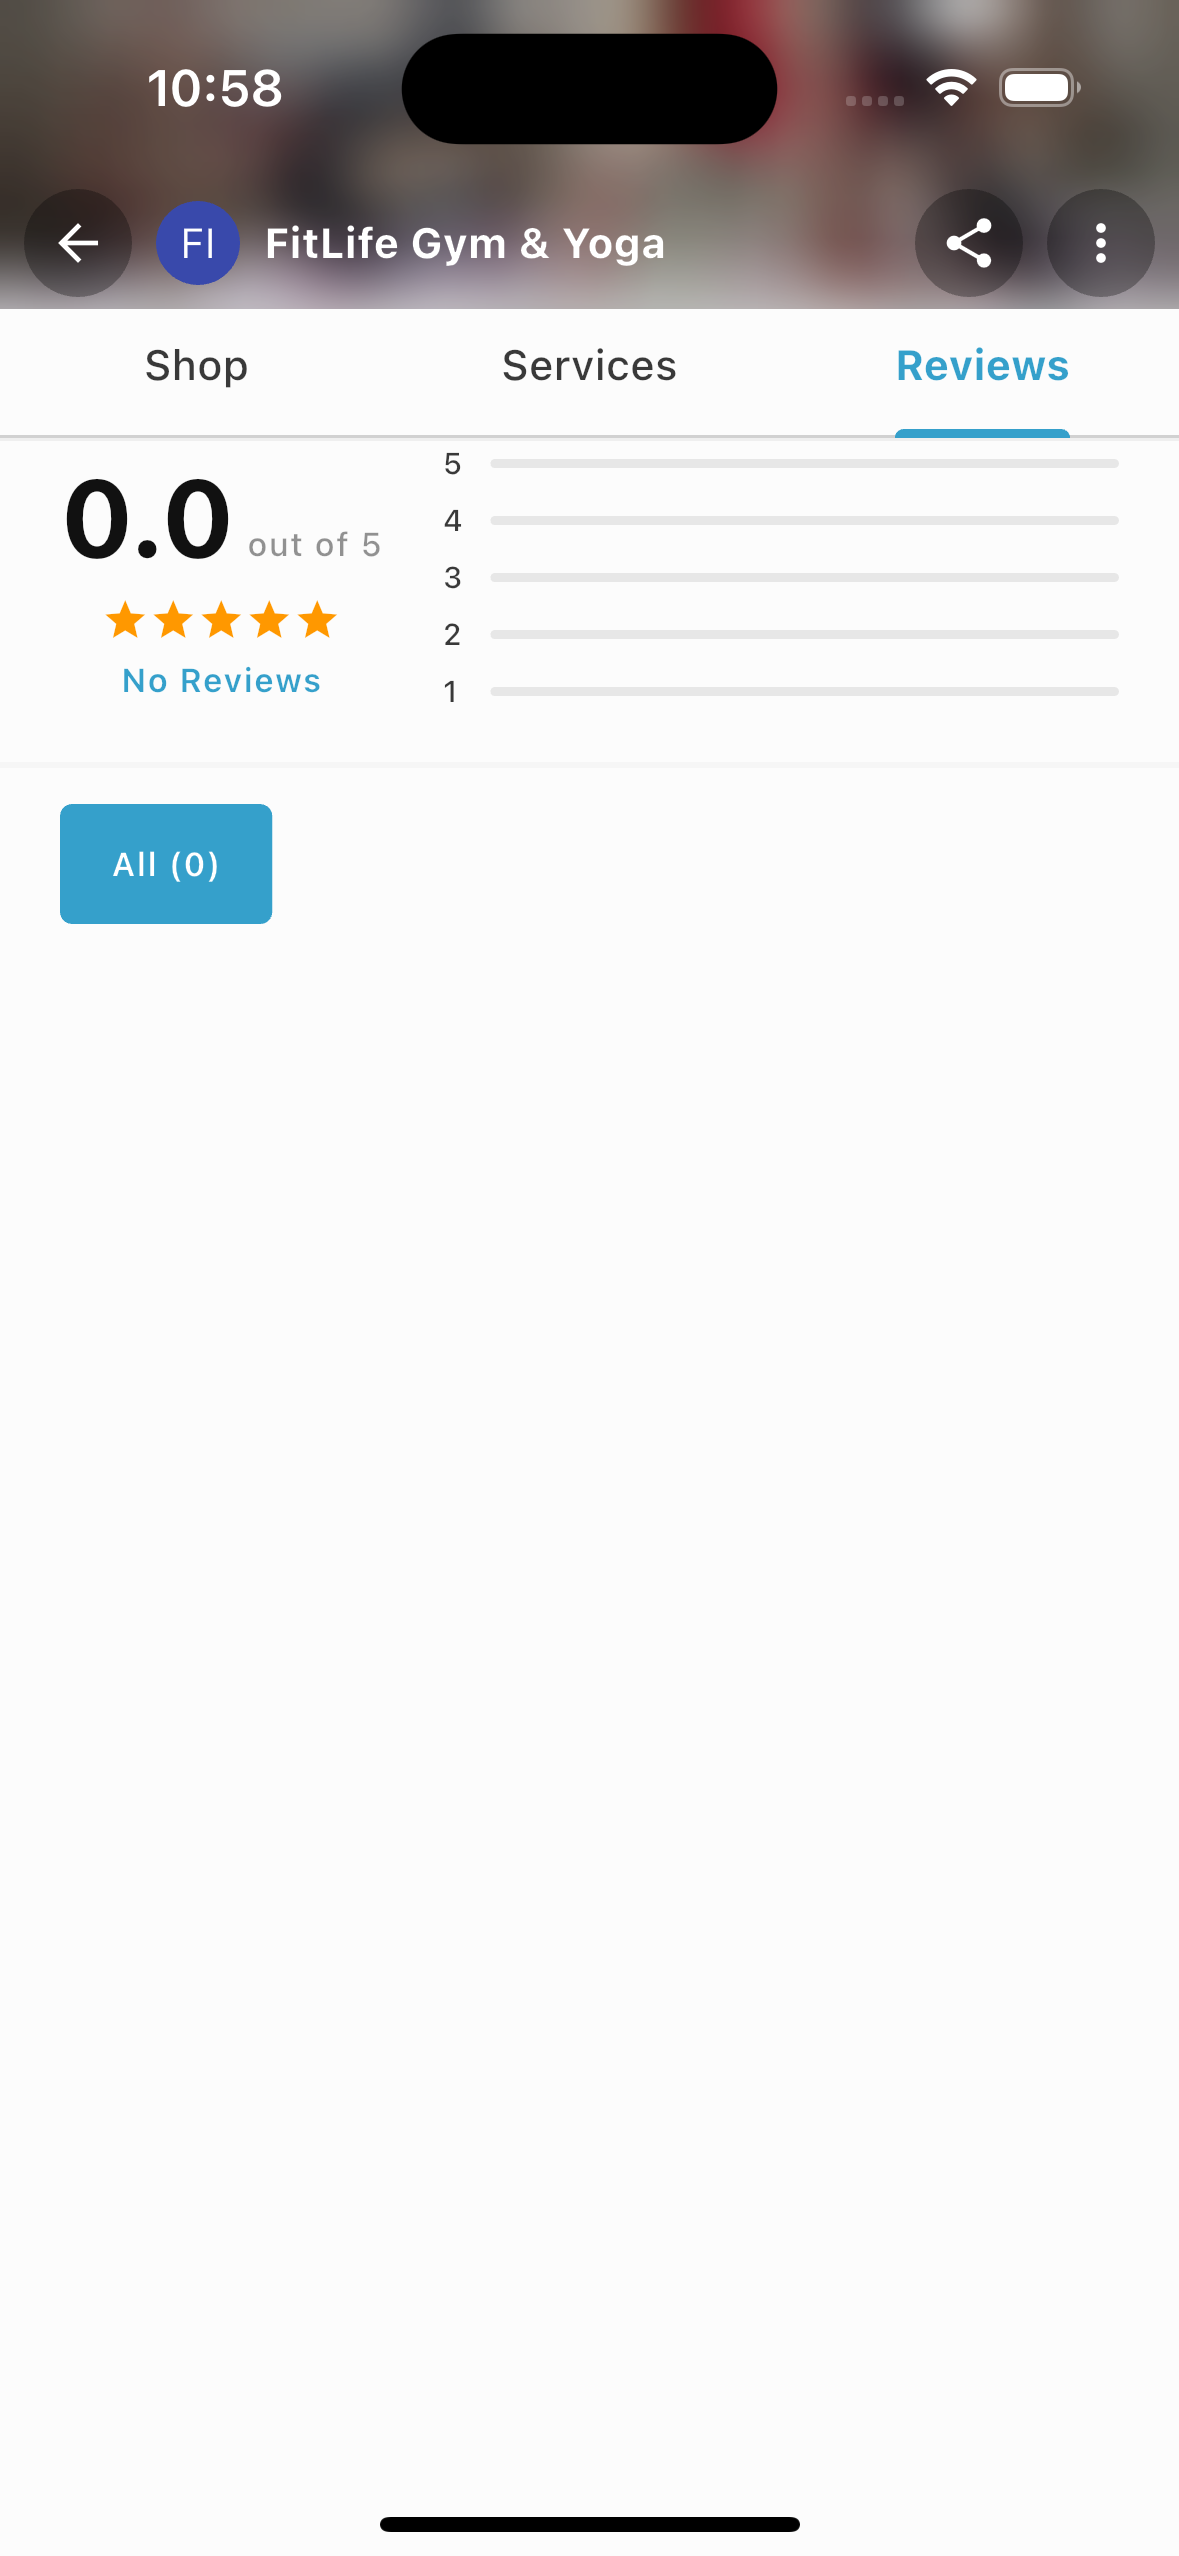
\includegraphics[width=\linewidth,height=0.38\textheight,keepaspectratio]{Images/Hiện thực/user_app/clinic_info/fig_clinic_info_4.png}
    \caption{Tab Đánh giá}
    \label{fig:clinic_info_reviews}
\end{subfigure}
\par\medskip
\caption{Trang chi tiết phòng khám với 3 tab: Cửa hàng, Dịch vụ, Đánh giá}
\label{fig:user_clinic_detail}
\end{figure}

\paragraph{Module Danh mục (\texttt{CategoriesModule})}

Tổ chức danh mục theo cấu trúc phân cấp parent-child (ví dụ: Y tế $\rightarrow$ Tim mạch $\rightarrow$ Khám tổng quát). \texttt{CategoriesController} cung cấp API công khai (không yêu cầu xác thực), trả danh sách kèm cấu trúc cây phục vụ hiển thị menu đa cấp trên ứng dụng.

\paragraph{Module Tags dịch vụ (\texttt{ServiceTagsModule})}

Quản lý hệ thống tags gắn với dịch vụ (\textit{yoga}, \textit{giảm cân}, \textit{tim mạch}). Quan hệ many-to-many với \texttt{Product}, hỗ trợ tìm kiếm đa chiều. API cho phép lọc dịch vụ theo tổ hợp tags.

\subsubsection{Tìm kiếm theo Vị trí}

\paragraph{Module Địa chỉ hành chính (\texttt{LocationsModule})}

Quản lý hệ thống địa chỉ phân cấp theo chuẩn hành chính Việt Nam: Tỉnh/Thành phố $\rightarrow$ Quận/Huyện $\rightarrow$ Phường/Xã (\texttt{LocationLevel} enum). Phục vụ validation địa chỉ khi đăng ký đối tác, tạo phòng khám và lưu địa chỉ người dùng.

\paragraph{Module Bản đồ (\texttt{MapboxModule})}

Tích hợp Mapbox API: Geocoding (địa chỉ $\leftrightarrow$ tọa độ), tìm kiếm theo vị trí với bán kính tùy chỉnh, và tính khoảng cách giữa hai điểm phục vụ sắp xếp kết quả.

\subsubsection{Chat thời gian thực (phía Người dùng)}

Nhắn tin thời gian thực giữa người dùng và đối tác, kết hợp REST API và WebSocket:

\begin{itemize}
    \item \textbf{Kiến trúc:} \texttt{UserChatController} (REST) + \texttt{UserChatGateway} (WebSocket).
    \item \textbf{Xác thực WebSocket:} Middleware \texttt{ws-jwt-auth} xác thực JWT khi thiết lập kết nối.
    \item \textbf{Dữ liệu:} \texttt{Conversation}/\texttt{ChatMessage} (nội dung, thời gian, trạng thái đã đọc).
    \item \textbf{REST bổ trợ:} Lịch sử tin nhắn (phân trang), danh sách cuộc trò chuyện, đánh dấu đã đọc.
\end{itemize}

% Placeholder: Uncomment khi có ảnh chụp màn hình chat
% \begin{figure}[H]
%     \centering
%     \begin{subfigure}[t]{0.3\textwidth}
%         \centering
%         \includegraphics[width=\linewidth]{Images/Hiện thực/fig_user_chat_list.png}
%         \caption{Danh sách cuộc trò chuyện}
%     \end{subfigure}
%     \hfill
%     \begin{subfigure}[t]{0.3\textwidth}
%         \centering
%         \includegraphics[width=\linewidth]{Images/Hiện thực/fig_user_chat_box.png}
%         \caption{Chat với đối tác}
%     \end{subfigure}
%     \hfill
%     \begin{subfigure}[t]{0.3\textwidth}
%         \centering
%         \includegraphics[width=\linewidth]{Images/Hiện thực/fig_user_ai_chat.png}
%         \caption{Chat với AI Chatbot}
%     \end{subfigure}
%     \caption{Giao diện Chat thời gian thực và tương tác với AI Chatbot}
%     \label{fig:user_chat_flow}
% \end{figure}

\subsubsection{Đánh giá dịch vụ (\texttt{ReviewModule})}

Phân hệ đánh giá cho phép người dùng để lại nhận xét và điểm số sau khi trải nghiệm dịch vụ. Quy trình được thiết kế theo dạng từng bước (step-by-step) nhằm tối ưu tỷ lệ hoàn thành khảo sát. Hệ thống thu thập hai luồng dữ liệu chính: \texttt{SpecialistReview} (đánh giá chuyên gia về chuyên môn, thái độ) và \texttt{TreatmentReview} (đánh giá trải nghiệm điều trị, không gian, kèm ảnh chụp thực tế qua \texttt{photo\_urls} jsonb). Điểm trung bình được tổng hợp và hiển thị trực tiếp trên trang chi tiết phòng khám.

\begin{enumerate}
    \item \textbf{Đánh giá dịch vụ:} Người dùng chấm điểm mức độ hài lòng về dịch vụ tổng thể.
    \item \textbf{Đánh giá chuyên gia \& cơ sở:} Hệ thống yêu cầu đánh giá chi tiết cho chuyên gia phụ trách và cơ sở vật chất.
    \item \textbf{Nhận xét và hình ảnh:} Người dùng nhập bình luận và có thể tải lên hình ảnh đính kèm (ảnh sau điều trị, hóa đơn).
    \item \textbf{Hoàn tất:} Sau khi gửi, hệ thống ghi nhận đánh giá và hiển thị màn hình thông báo thành công.
\end{enumerate}

\begin{figure}[H]
\centering
\captionsetup[subfigure]{font=small,justification=centering}
\captionsetup{skip=8pt}
\begin{subfigure}[t]{0.48\linewidth}
    \centering
    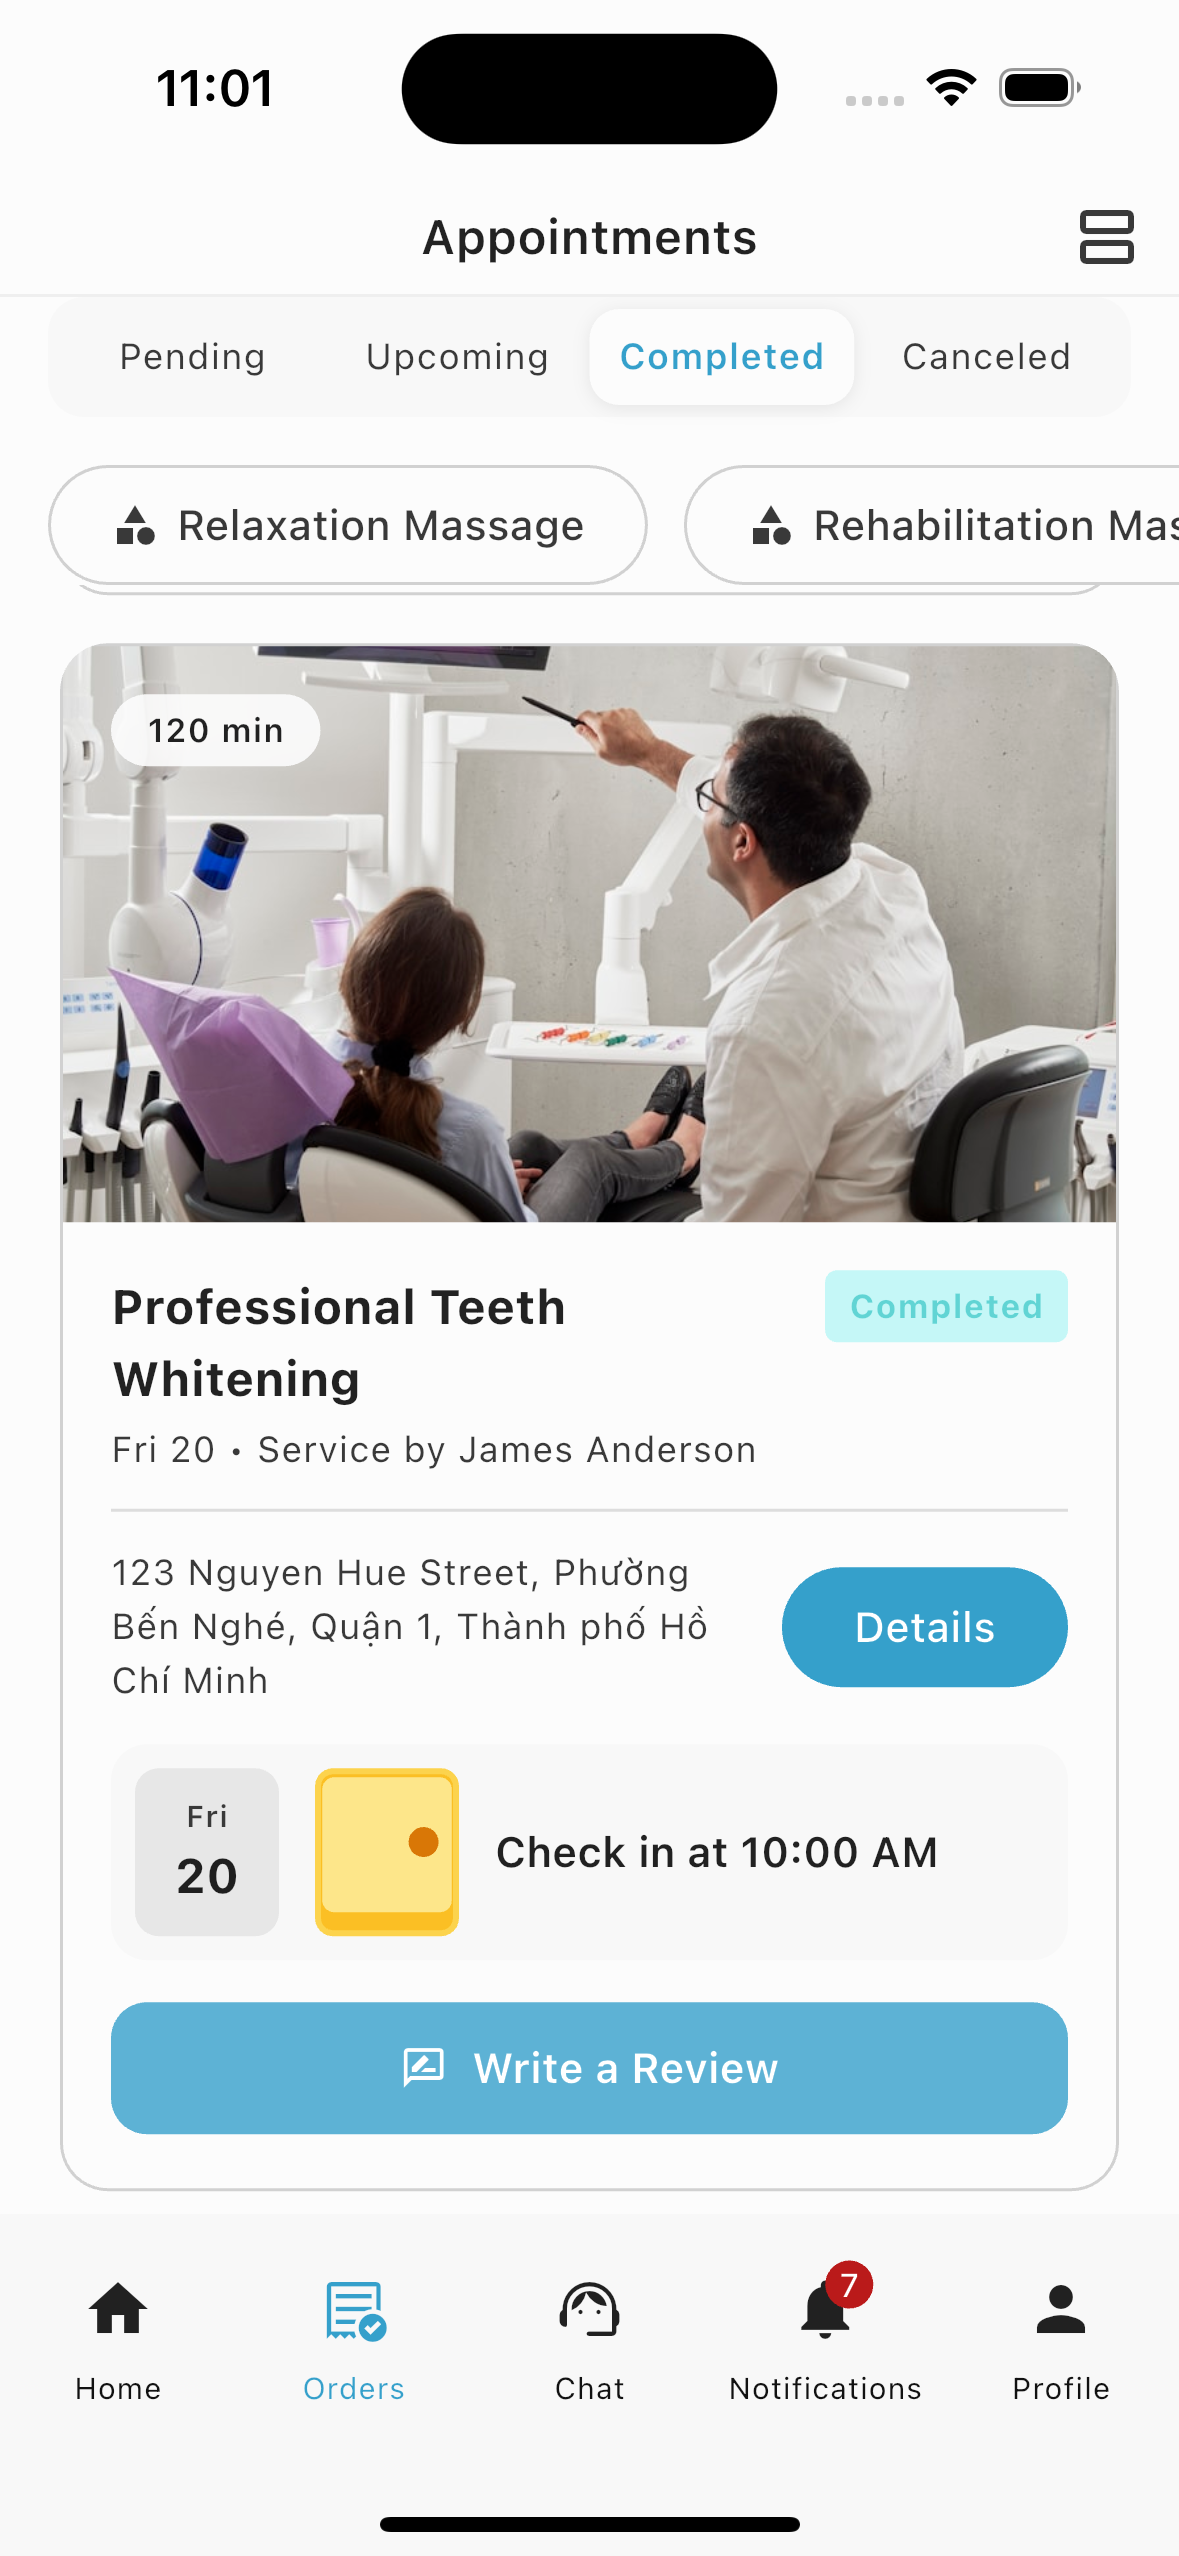
\includegraphics[width=\linewidth,height=0.35\textheight,keepaspectratio]{Images/Hiện thực/user_app/reviews/fig_review_step1.png}
    \caption{Bắt đầu đánh giá dịch vụ}
    \label{fig:review_step1}
\end{subfigure}
\hfill
\begin{subfigure}[t]{0.48\linewidth}
    \centering
    
\includegraphics[width=\linewidth,height=0.35\textheight,keepaspectratio]{Images/Hiện thực/user_app/reviews/fig_review_step2.png}
    \caption{Đánh giá chuyên gia}
    \label{fig:review_step2}
\end{subfigure}
\par\medskip
\begin{subfigure}[t]{0.48\linewidth}
    \centering
    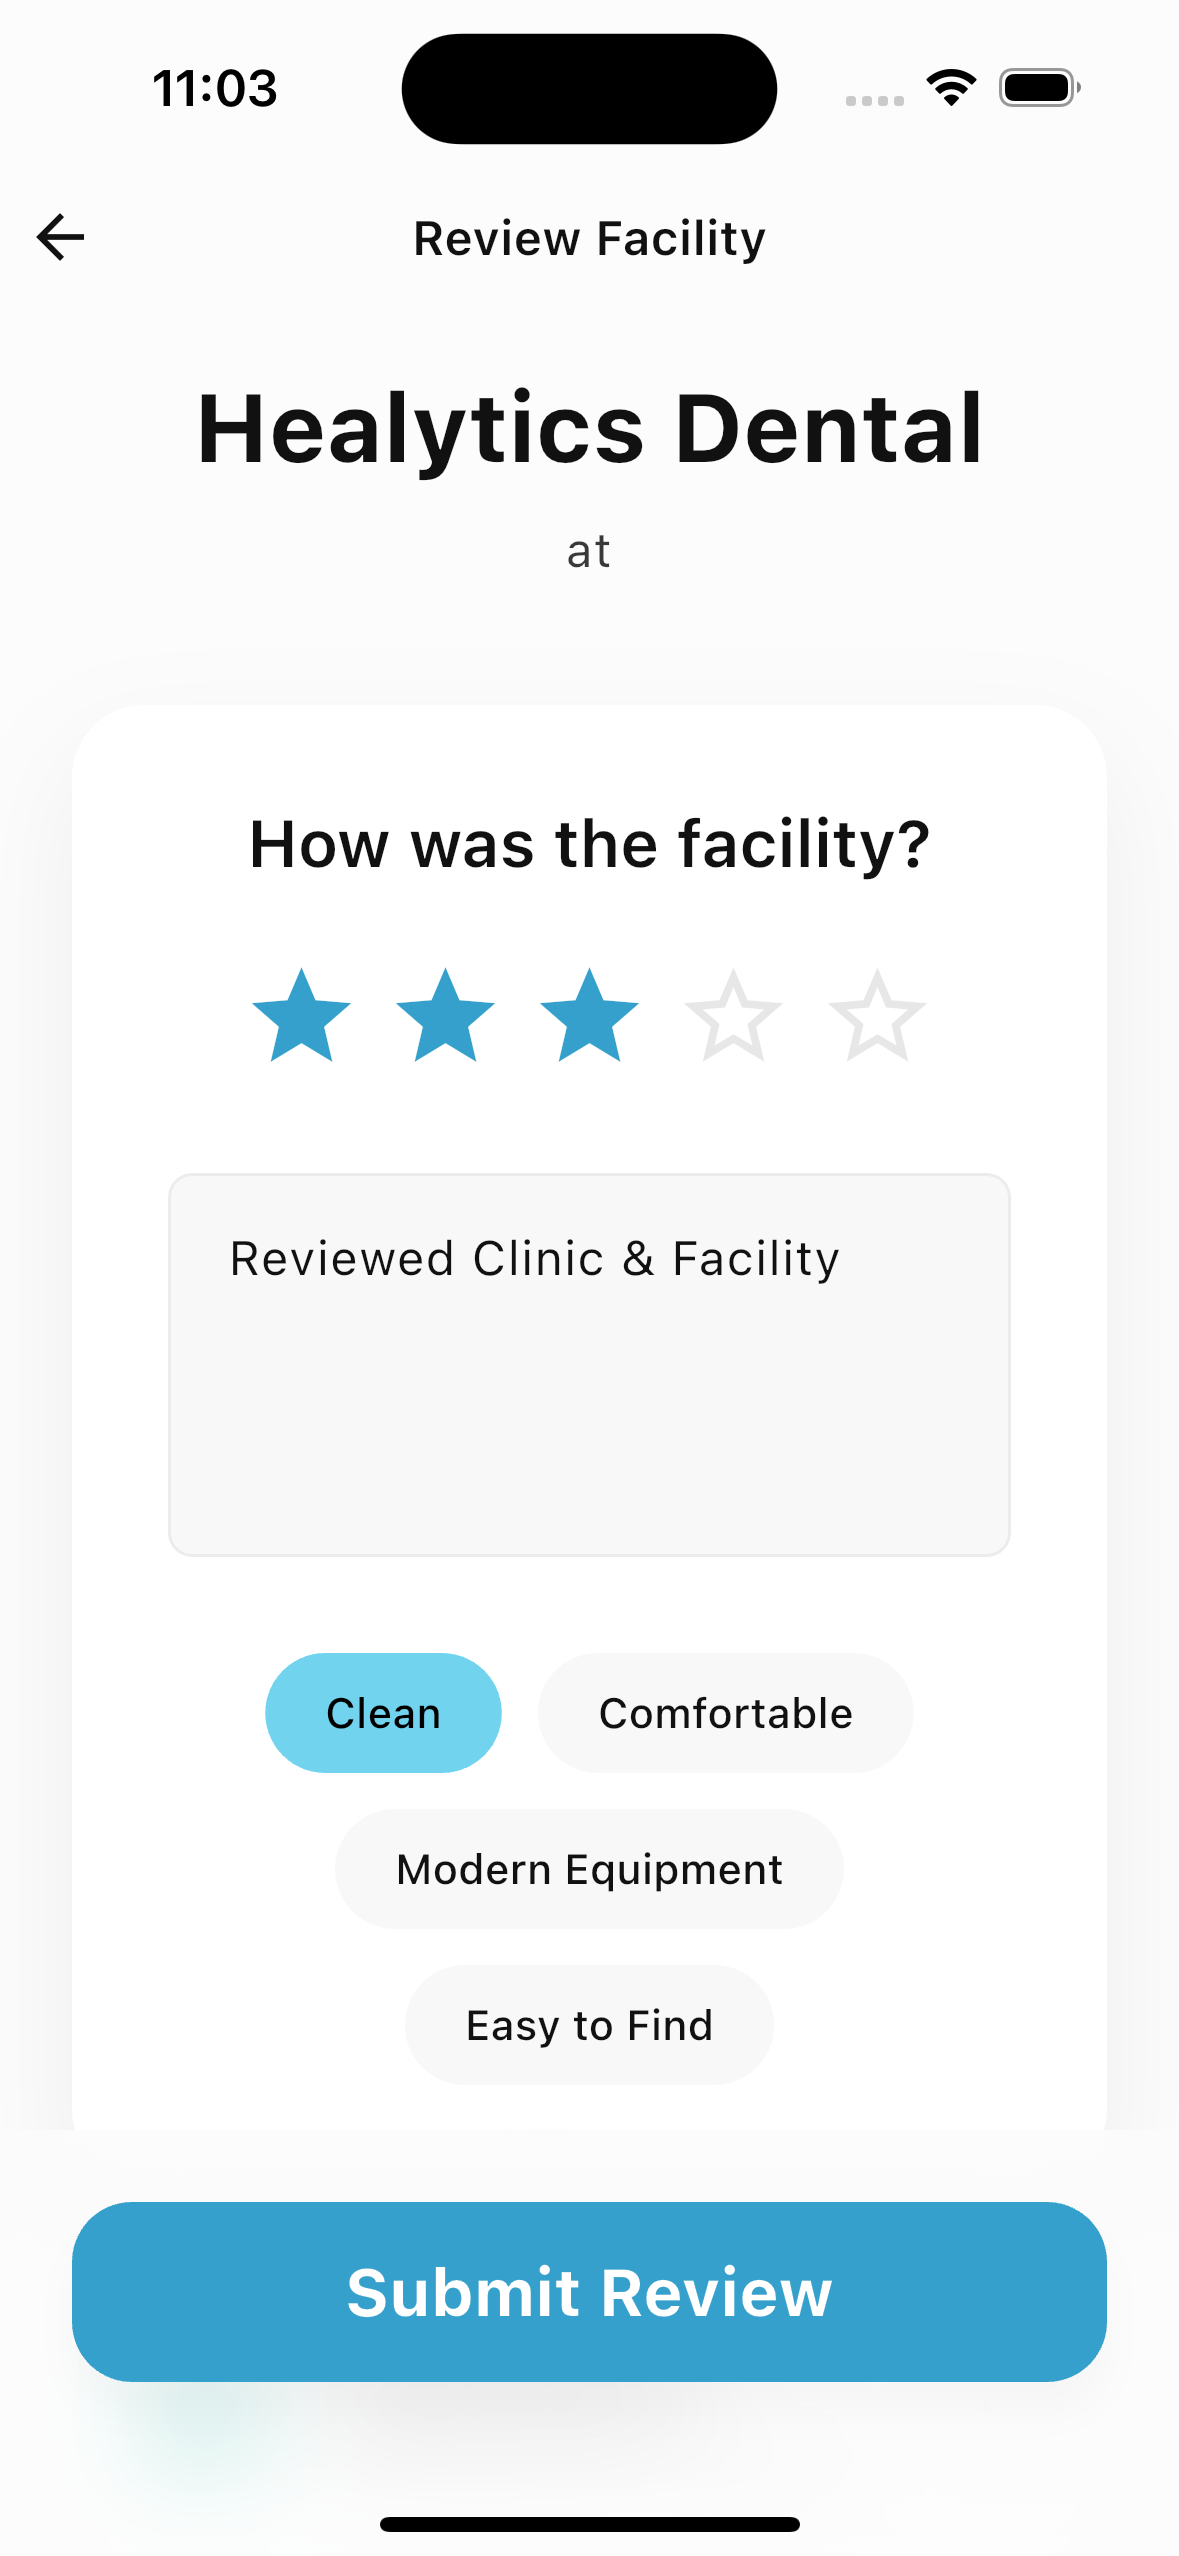
\includegraphics[width=\linewidth,height=0.35\textheight,keepaspectratio]{Images/Hiện thực/user_app/reviews/fig_review_step3.png}
    \caption{Nhận xét chi tiết và đính kèm ảnh}
    \label{fig:review_step3}
\end{subfigure}
\hfill
\begin{subfigure}[t]{0.48\linewidth}
    \centering
    
\includegraphics[width=\linewidth,height=0.35\textheight,keepaspectratio]{Images/Hiện thực/user_app/reviews/fig_review_step4.png}
    \caption{Hoàn tất đánh giá}
    \label{fig:review_step4}
\end{subfigure}
\par\medskip
\caption{Luồng Đánh giá dịch vụ (Service Review) trên ứng dụng người bệnh}
\label{fig:user_review_flow}
\end{figure}

\subsubsection{Quản lý Đặt lịch, Giỏ hàng và Thanh toán}

\paragraph{Module Đặt lịch (\texttt{BookingModule})}

Xử lý quy trình đặt lịch theo mô hình máy trạng thái:

\begin{itemize}
    \item \textbf{Luồng trạng thái:} \texttt{PENDING\_PAYMENT} $\rightarrow$ \texttt{CONFIRMED} $\rightarrow$ \texttt{IN\_PROGRESS} $\rightarrow$ \texttt{COMPLETED} hoặc \texttt{CANCELLED}. Mỗi chuyển trạng thái được ghi vào \texttt{BookingStatusLog} kèm actor, lý do, và timestamp.
    \item \textbf{Quản lý slot:} \texttt{SlotsController} kiểm tra khung giờ trống, ngăn double-booking qua khóa phân tán Redis.
    \item \textbf{Tích hợp thanh toán:} Booking xác nhận tự động kích hoạt thanh toán qua \texttt{BookingPaymentService}.
\end{itemize}

% Placeholder: Uncomment khi có ảnh chụp màn hình đặt lịch
\subsubsection{Kiến trúc giao diện User Portal}

\paragraph{Màn hình chính (Home)}

Màn hình chính là điểm khởi đầu của người dùng, cung cấp truy cập nhanh đến các tính năng chính:

\begin{figure}[H]
\centering
\captionsetup[subfigure]{font=small,justification=centering}
\captionsetup{skip=6pt}
\begin{subfigure}[t]{0.48\linewidth}
    \centering
    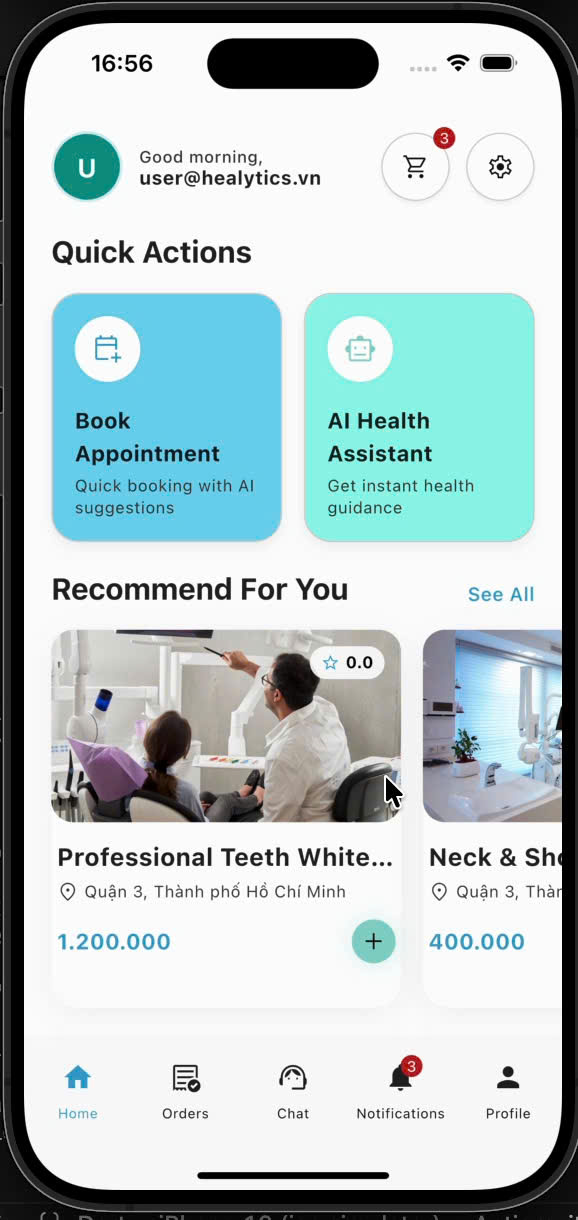
\includegraphics[width=\linewidth,height=0.4\textheight,keepaspectratio]{Images/Hiện thực/user/fig_user_home.jpg}
    \caption{Giao diện chế độ sáng với Quick Actions và Recommend For You}
    \label{fig:user_home_home}
\end{subfigure}
\hfill
\begin{subfigure}[t]{0.48\linewidth}
    \centering
    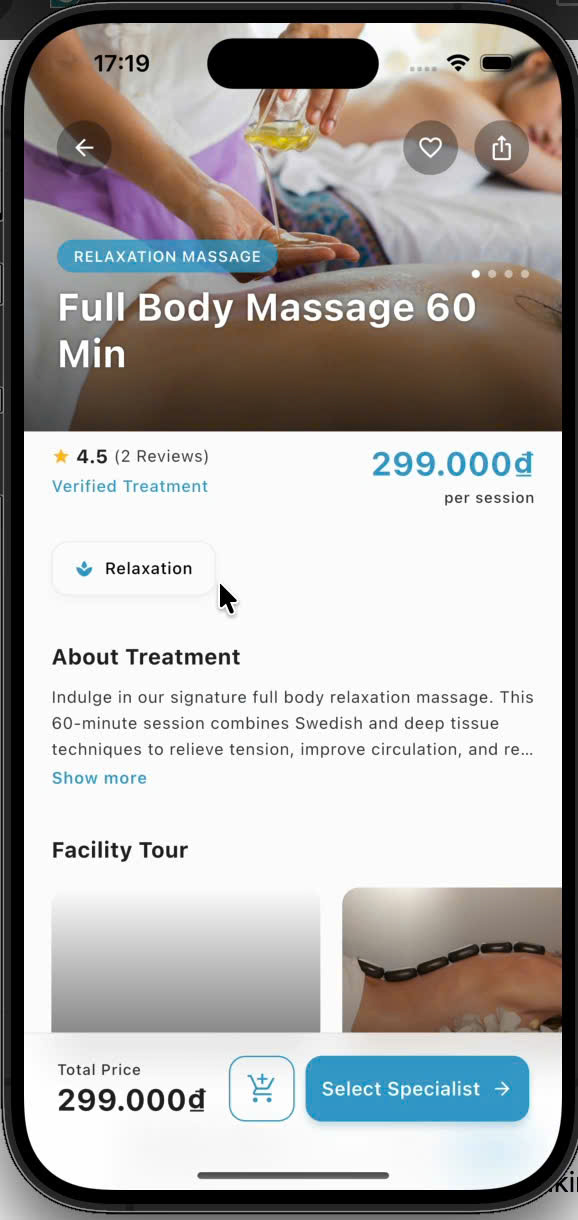
\includegraphics[width=\linewidth,height=0.4\textheight,keepaspectratio]{Images/Hiện thực/user/fig_user_service_detail.jpg}
    \caption{Chi tiết dịch vụ được đề xuất}
    \label{fig:user_home_service_detail}
\end{subfigure}
\par\medskip
\caption{Màn hình Home - Trung tâm của User Portal}
\label{fig:user_home}
\end{figure}

\begin{itemize}
    \item \textbf{Thao tác chính:} Người dùng chọn nhanh \textit{Book Appointment} hoặc \textit{AI Health Assistant} từ khối Quick Actions.
    \item \textbf{Thao tác điều hướng:} Nhấn các tab ở thanh dưới để chuyển giữa Home, Orders, Chat, Notifications và Profile.
\end{itemize}

\textbf{Thành phần chính:}

\begin{itemize}
    \item \textbf{User Profile Header:} Hiển thị tên người dùng, icon settings, và giỏ hàng.
    \item \textbf{Quick Actions:} Book Appointment và AI Health Assistant.
    \item \textbf{Recommend For You:} Carousel dịch vụ được khuyến nghị.
    \item \textbf{Bottom Navigation:} 5 tab: Home, Orders, Chat, Notifications, Profile.
\end{itemize}

\textbf{Tính năng kỹ thuật:}

\begin{itemize}
    \item \textbf{State Management:} BLoC pattern cho danh sách recommended.
    \item \textbf{Caching:} Tránh reload không cần thiết.
    \item \textbf{Pull-to-Refresh:} Làm mới danh sách dịch vụ.
\end{itemize}

\paragraph{Quản lý lịch hẹn (Appointments)}

Màn hình Appointments cho phép người dùng theo dõi toàn bộ lịch sử hẹn được phân loại thành bốn tab: Pending (chờ thanh toán), Upcoming (sắp tới), Completed (hoàn thành), và Canceled (đã hủy). Mỗi lịch hẹn được hiển thị dưới dạng card chứa thông tin dịch vụ, cơ sở y tế, chuyên gia, thời gian check-in, và trạng thái thanh toán. Người dùng có thể nhấn nút \textit{Details} để xem chi tiết đầy đủ hoặc thực hiện các hành động bổ sung.

\begin{figure}[H]
\centering
\captionsetup[subfigure]{font=small,justification=centering}
\captionsetup{skip=6pt}
\begin{subfigure}[t]{0.48\linewidth}
    \centering
    \includegraphics[width=\linewidth,height=0.36\textheight,keepaspectratio]{Images/Hiện thực/user_app/appoinment/fig_appointment_pending.png}
    \caption{Tab Pending -- chờ thanh toán}
    \label{fig:appointment_pending}
\end{subfigure}
\hfill
\begin{subfigure}[t]{0.48\linewidth}
    \centering
    \includegraphics[width=\linewidth,height=0.36\textheight,keepaspectratio]{Images/Hiện thực/user_app/appoinment/fig_appointment_upcoming.png}
    \caption{Tab Upcoming -- lịch hẹn sắp tới}
    \label{fig:appointment_upcoming}
\end{subfigure}
\par\medskip
\caption{Quản lý lịch hẹn -- danh sách hẹn theo trạng thái}
\label{fig:appointments_list}
\end{figure}

\textbf{Tính năng kỹ thuật:}

\begin{itemize}
    \item \textbf{Phân loại theo trạng thái:} Bốn tab (Pending, Upcoming, Completed, Canceled) với lazy loading 10 item/batch.
    \item \textbf{Real-time Status Sync:} WebSocket cập nhật trạng thái lịch hẹn khi có thay đổi từ phía partner.
    \item \textbf{Push Notification:} Nhắc nhở 1 giờ trước lịch hẹn qua FCM.
\end{itemize}

\paragraph{Xem chi tiết lịch hẹn và Hướng dẫn dịch vụ}

Khi người dùng nhấn nút \textit{Details} từ danh sách hẹn, màn hình Appointment Details hiển thị thông tin đầy đủ về lịch hẹn: hình ảnh dịch vụ, tên dịch vụ, cơ sở y tế, chuyên gia phụ trách, thời gian check-in/check-out, và các tùy chọn liên quan (xem hướng dẫn dịch vụ, nhắn tin với cơ sở). Người dùng có thể nhấn \textit{Service manual} để truy cập hướng dẫn chi tiết về dịch vụ, bao gồm: guidelines trước dịch vụ (Pre-Service Guidelines), các bước thực hiện dịch vụ, hình ảnh cơ sở vật chất (Facilities), và lịch sử đánh giá về dịch vụ đó. Tính năng này giúp người dùng chuẩn bị tốt trước cuộc hẹn và giao tiếp trực tiếp với nhân viên qua chat.

\begin{figure}[H]
\centering
\captionsetup[subfigure]{font=small,justification=centering}
\captionsetup{skip=6pt}
\begin{subfigure}[t]{0.48\linewidth}
    \centering
    \includegraphics[width=\linewidth,height=0.36\textheight,keepaspectratio]{Images/Hiện thực/user_app/appoinment/fig_appointment_details.png}
    \caption{Chi tiết lịch hẹn}
    \label{fig:appointment_details}
\end{subfigure}
\hfill
\begin{subfigure}[t]{0.48\linewidth}
    \centering
    \includegraphics[width=\linewidth,height=0.36\textheight,keepaspectratio]{Images/Hiện thực/user_app/appoinment/fig_appointment_manual_1.png}
    \caption{Hướng dẫn dịch vụ -- phần 1}
    \label{fig:appointment_manual_part1}
\end{subfigure}
\par\medskip
\begin{subfigure}[t]{0.48\linewidth}
    \centering
    \includegraphics[width=\linewidth,height=0.36\textheight,keepaspectratio]{Images/Hiện thực/user_app/appoinment/fig_appointment_manual_2.png}
    \caption{Hướng dẫn dịch vụ -- phần 2}
    \label{fig:appointment_manual_part2}
\end{subfigure}
\hfill
\begin{subfigure}[t]{0.48\linewidth}
    \centering
    \includegraphics[width=\linewidth,height=0.36\textheight,keepaspectratio]{Images/Hiện thực/user_app/appoinment/fig_appointment_chat.png}
    \caption{Chat với cơ sở y tế}
    \label{fig:appointment_chat}
\end{subfigure}
\par\medskip
\caption{Chi tiết lịch hẹn, hướng dẫn dịch vụ, và liên hệ với cơ sở}
\label{fig:appointment_details_flow}
\end{figure}

\textbf{Thành phần chính của Service Manual:}

\begin{itemize}
    \item \textbf{Pre-Service Guidelines:} Hướng dẫn chuẩn bị trước dịch vụ (ví dụ: chải răng trước khi tẩy trắng, tránh cà phê 24 giờ trước).
    \item \textbf{Service Rules:} Quy tắc thực hiện dịch vụ từng bước (bao gồm numbered steps, icons minh họa).
    \item \textbf{Facilities:} Hình ảnh gallery các cơ sở vật chất, thiết bị sử dụng.
    \item \textbf{Review:} Tổng hợp đánh giá (số sao trung bình, danh sách feedback từ khách hàng trước).
\end{itemize}

\paragraph{Luồng đặt lịch hẹn (Book Appointment)}

Quy trình đặt lịch được tổ chức theo mô hình wizard 3 bước, mỗi bước hiển thị thanh tiến trình (progress bar) giúp người dùng nắm rõ vị trí hiện tại trong luồng:

\begin{enumerate}
    \item \textbf{Bước 1 -- Chọn danh mục và dịch vụ:} Người dùng tìm kiếm hoặc chọn danh mục sức khỏe (Dental Care, Dermatology, Fitness \& Yoga, v.v.) từ lưới biểu tượng. Sau khi chọn danh mục, danh sách dịch vụ thuộc danh mục đó hiển thị bên dưới kèm thông tin hình ảnh, thời lượng, giá và phòng khám cung cấp. Người dùng đánh dấu dịch vụ mong muốn rồi nhấn \textit{Continue}.

    \item \textbf{Bước 2 -- Chọn chuyên gia và lịch hẹn:} Hệ thống hiển thị danh sách chuyên gia đủ điều kiện (ảnh, tên, chuyên ngành). Người dùng chọn chuyên gia, sau đó chọn ngày từ dải lịch ngang và khung giờ khả dụng (Morning, Afternoon) được tải từ API slot. Các slot đã bị khóa phân tán (Redis Redlock) sẽ không xuất hiện.

    \item \textbf{Bước 3 -- Xác nhận đặt lịch:} Màn hình tổng hợp hiển thị thông tin chuyên gia, ngày giờ, danh mục và dịch vụ, địa chỉ phòng khám, cùng bảng chi phí (Subtotal, Discount, Total Amount). Người dùng nhấn \textit{Confirm \& Pay} để chuyển sang bước thanh toán.
\end{enumerate}

\begin{figure}[H]
\centering
\captionsetup[subfigure]{font=small,justification=centering}
\captionsetup{skip=8pt}
\begin{subfigure}[t]{0.48\linewidth}
    \centering
    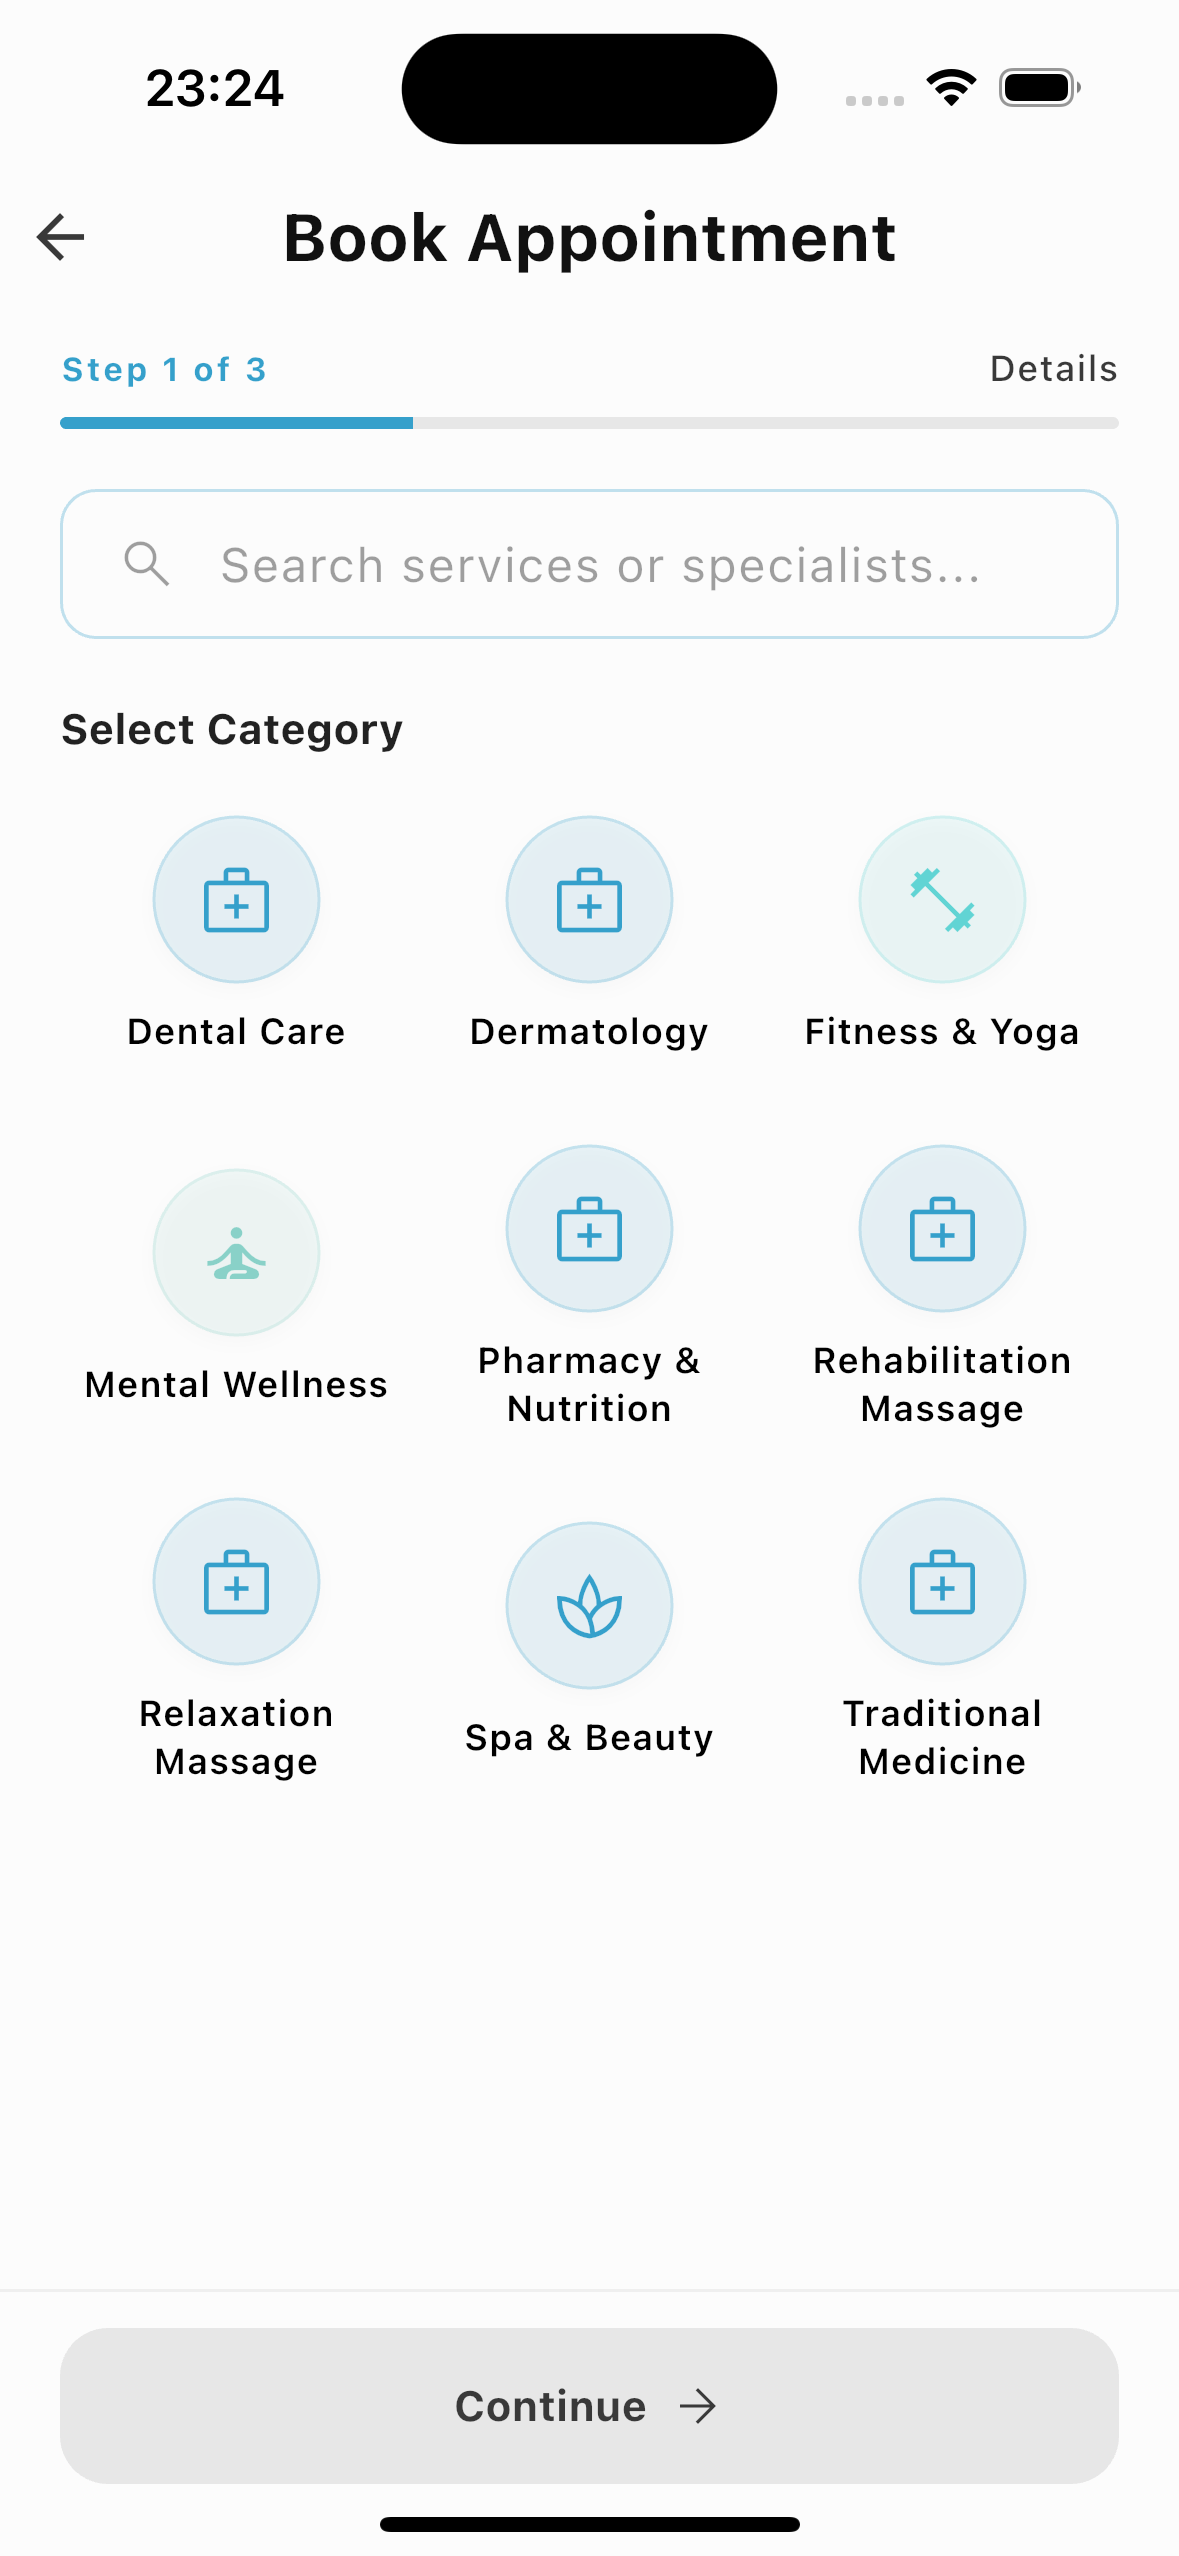
\includegraphics[width=\linewidth,height=0.28\textheight,keepaspectratio]{Images/Hiện thực/user_app/booking/fig_booking_step1_category.png}
    \caption{Chọn danh mục dịch vụ}
    \label{fig:booking_step1_category}
\end{subfigure}
\hfill
\begin{subfigure}[t]{0.48\linewidth}
    \centering
    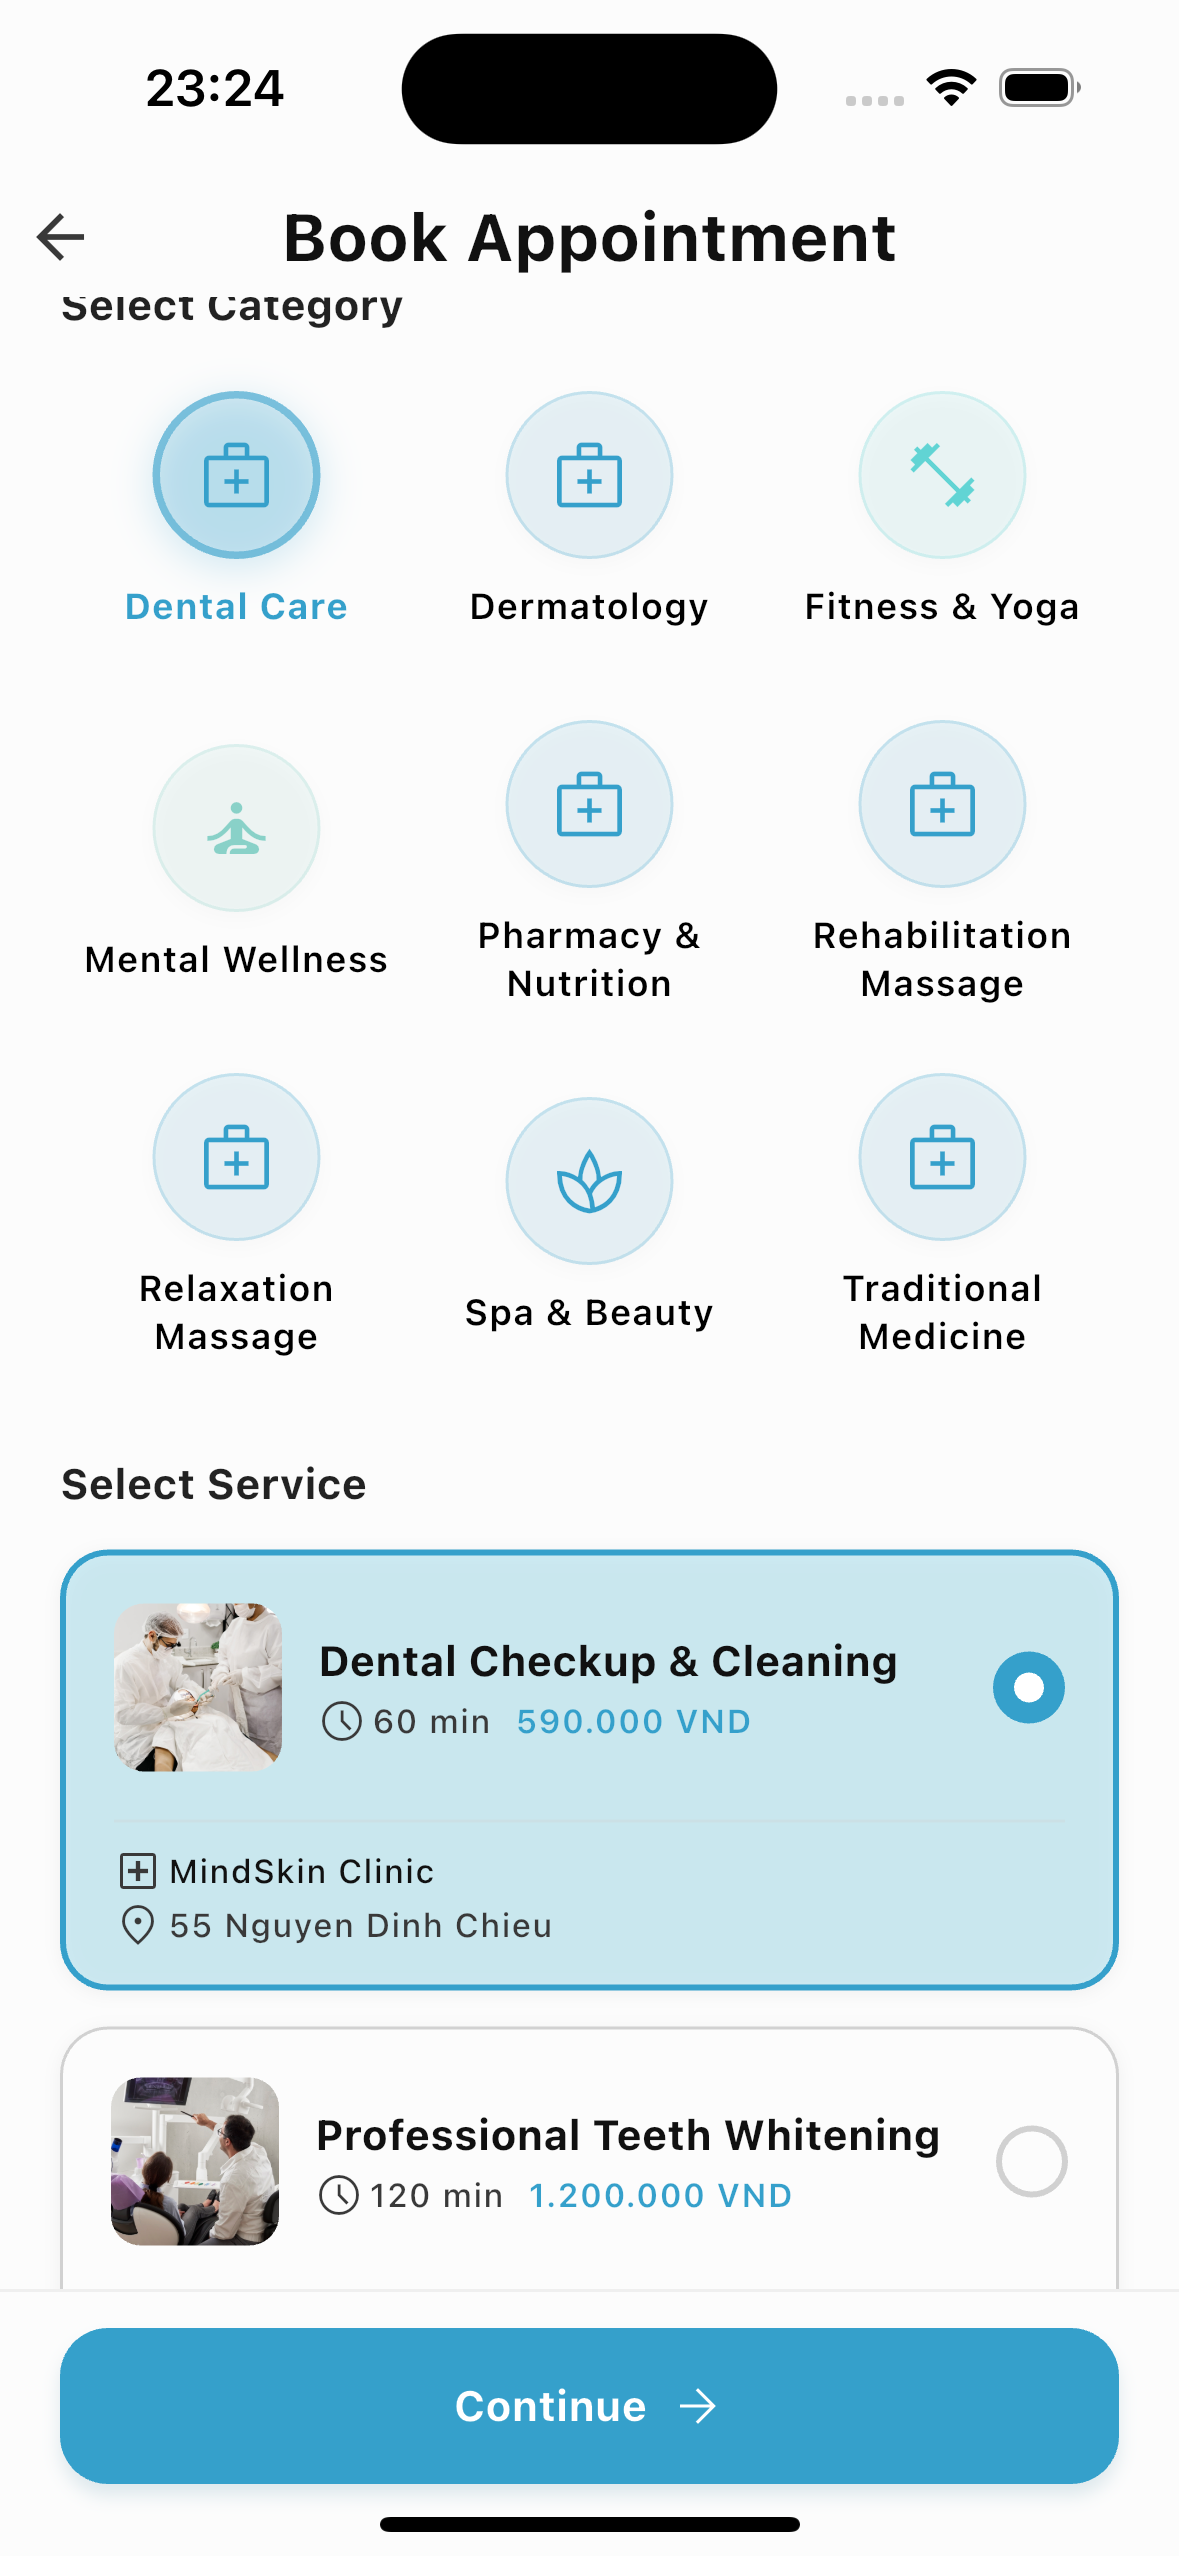
\includegraphics[width=\linewidth,height=0.28\textheight,keepaspectratio]{Images/Hiện thực/user_app/booking/fig_booking_step1_service.png}
    \caption{Chọn dịch vụ sau khi lọc danh mục}
    \label{fig:booking_step1_service}
\end{subfigure}
\par\medskip
\caption{Bước 1 -- Chọn danh mục và dịch vụ trong luồng Book Appointment}
\label{fig:booking_step1}
\end{figure}

\begin{figure}[H]
\centering
\captionsetup[subfigure]{font=small,justification=centering}
\captionsetup{skip=8pt}
\begin{subfigure}[t]{0.48\linewidth}
    \centering
    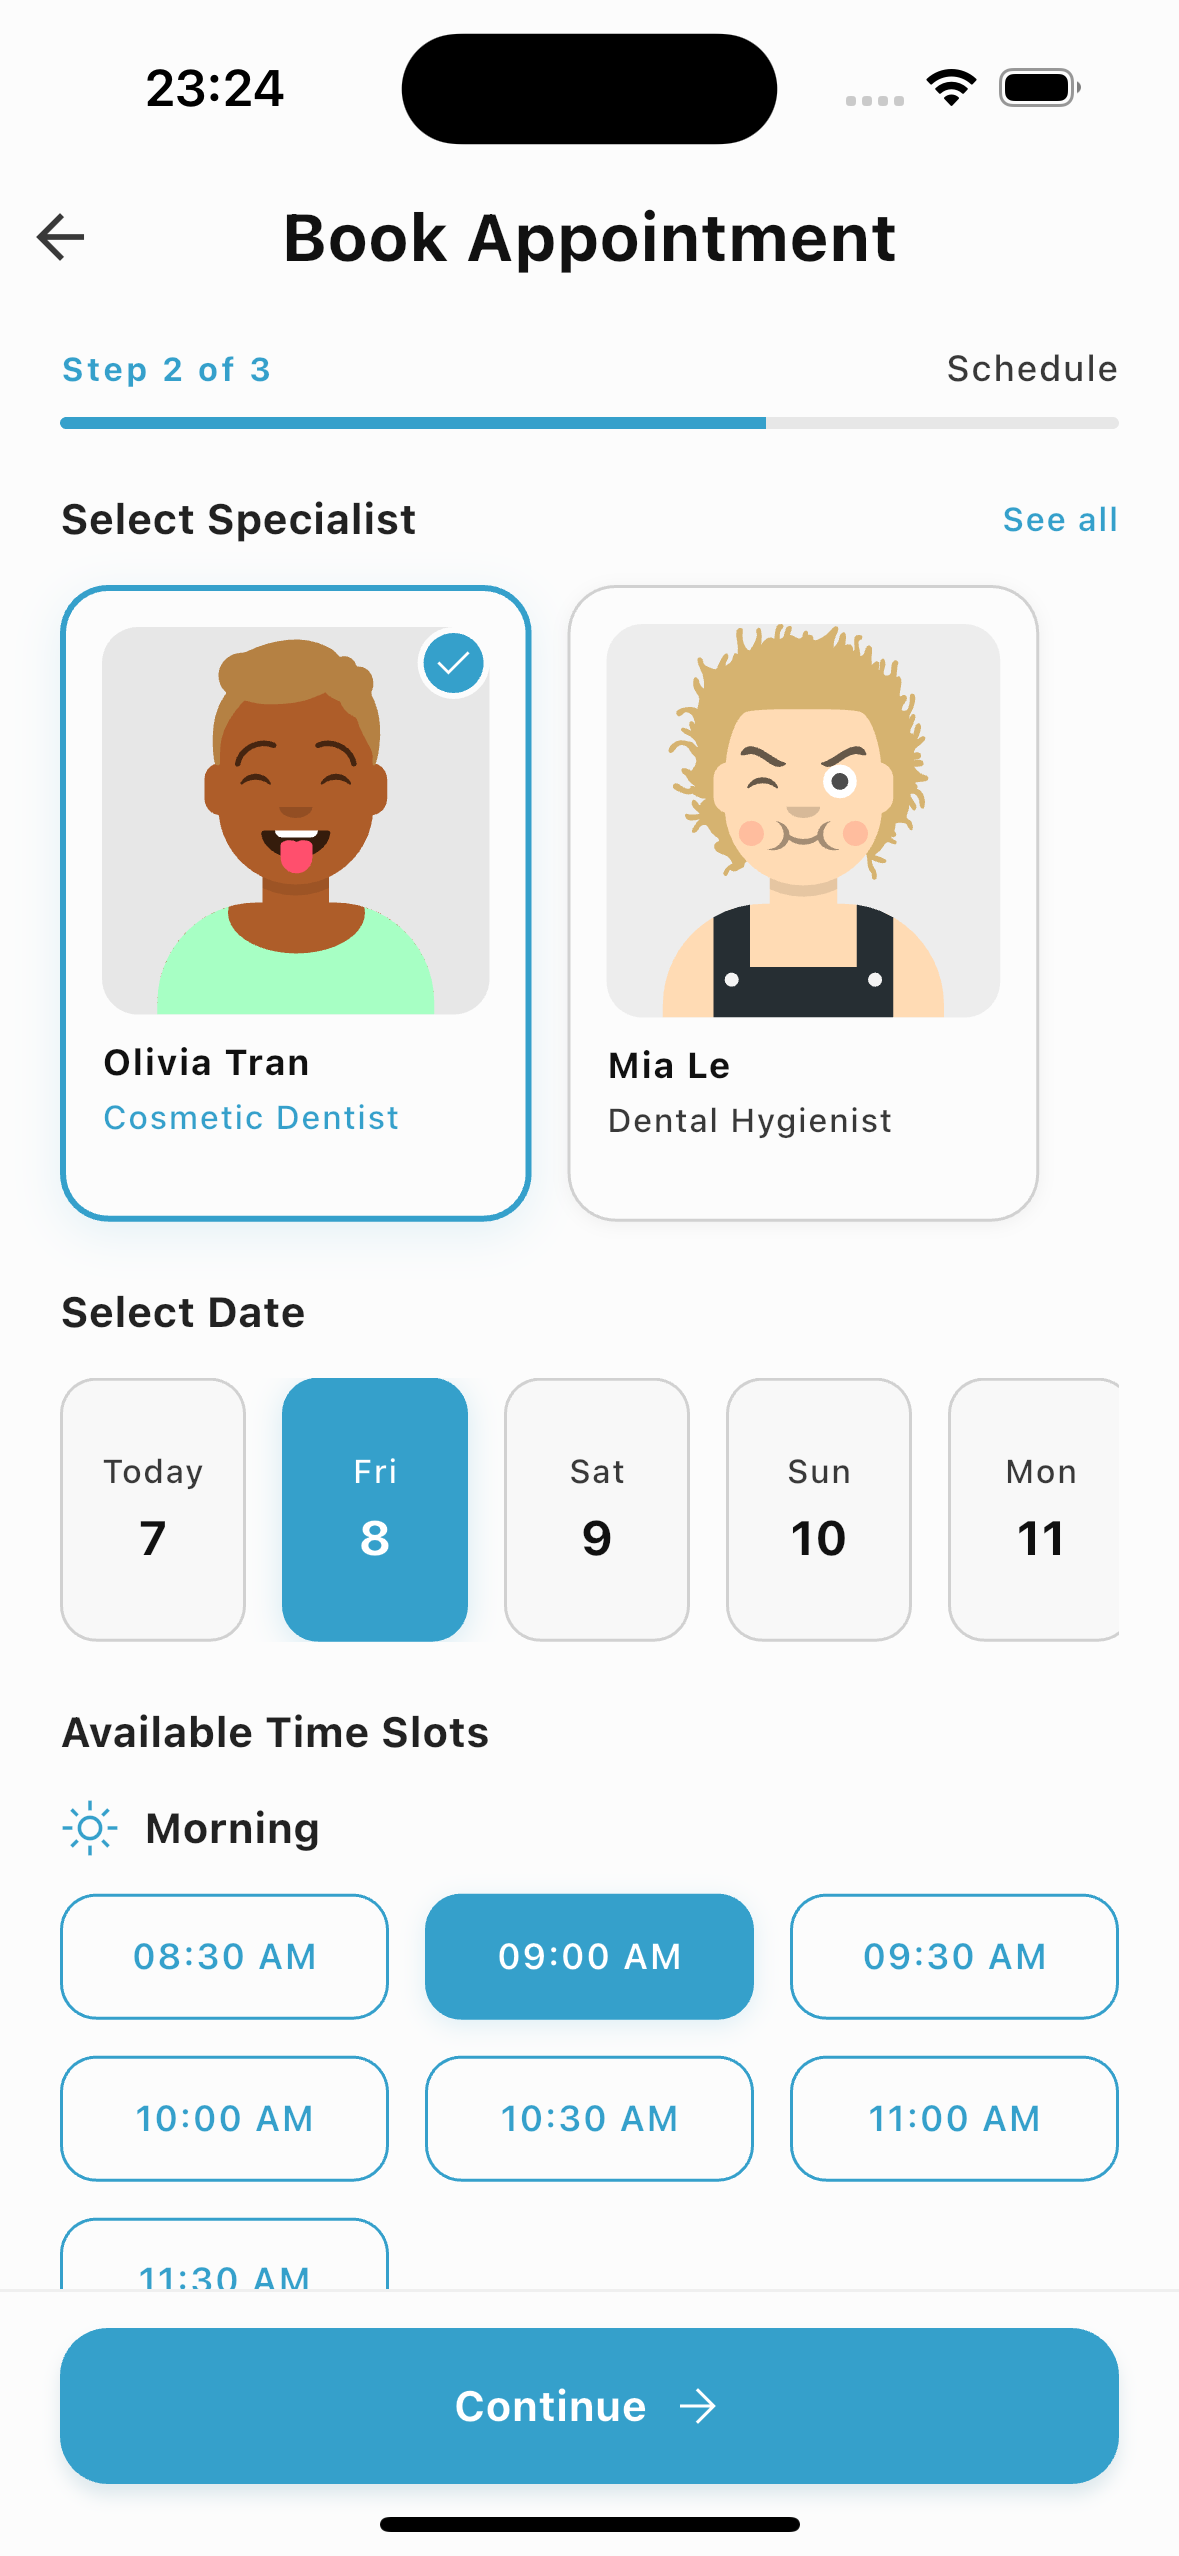
\includegraphics[width=\linewidth,height=0.28\textheight,keepaspectratio]{Images/Hiện thực/user_app/booking/fig_booking_step2_schedule.png}
    \caption{Chọn chuyên gia, ngày và khung giờ}
    \label{fig:booking_step2_schedule}
\end{subfigure}
\hfill
\begin{subfigure}[t]{0.48\linewidth}
    \centering
    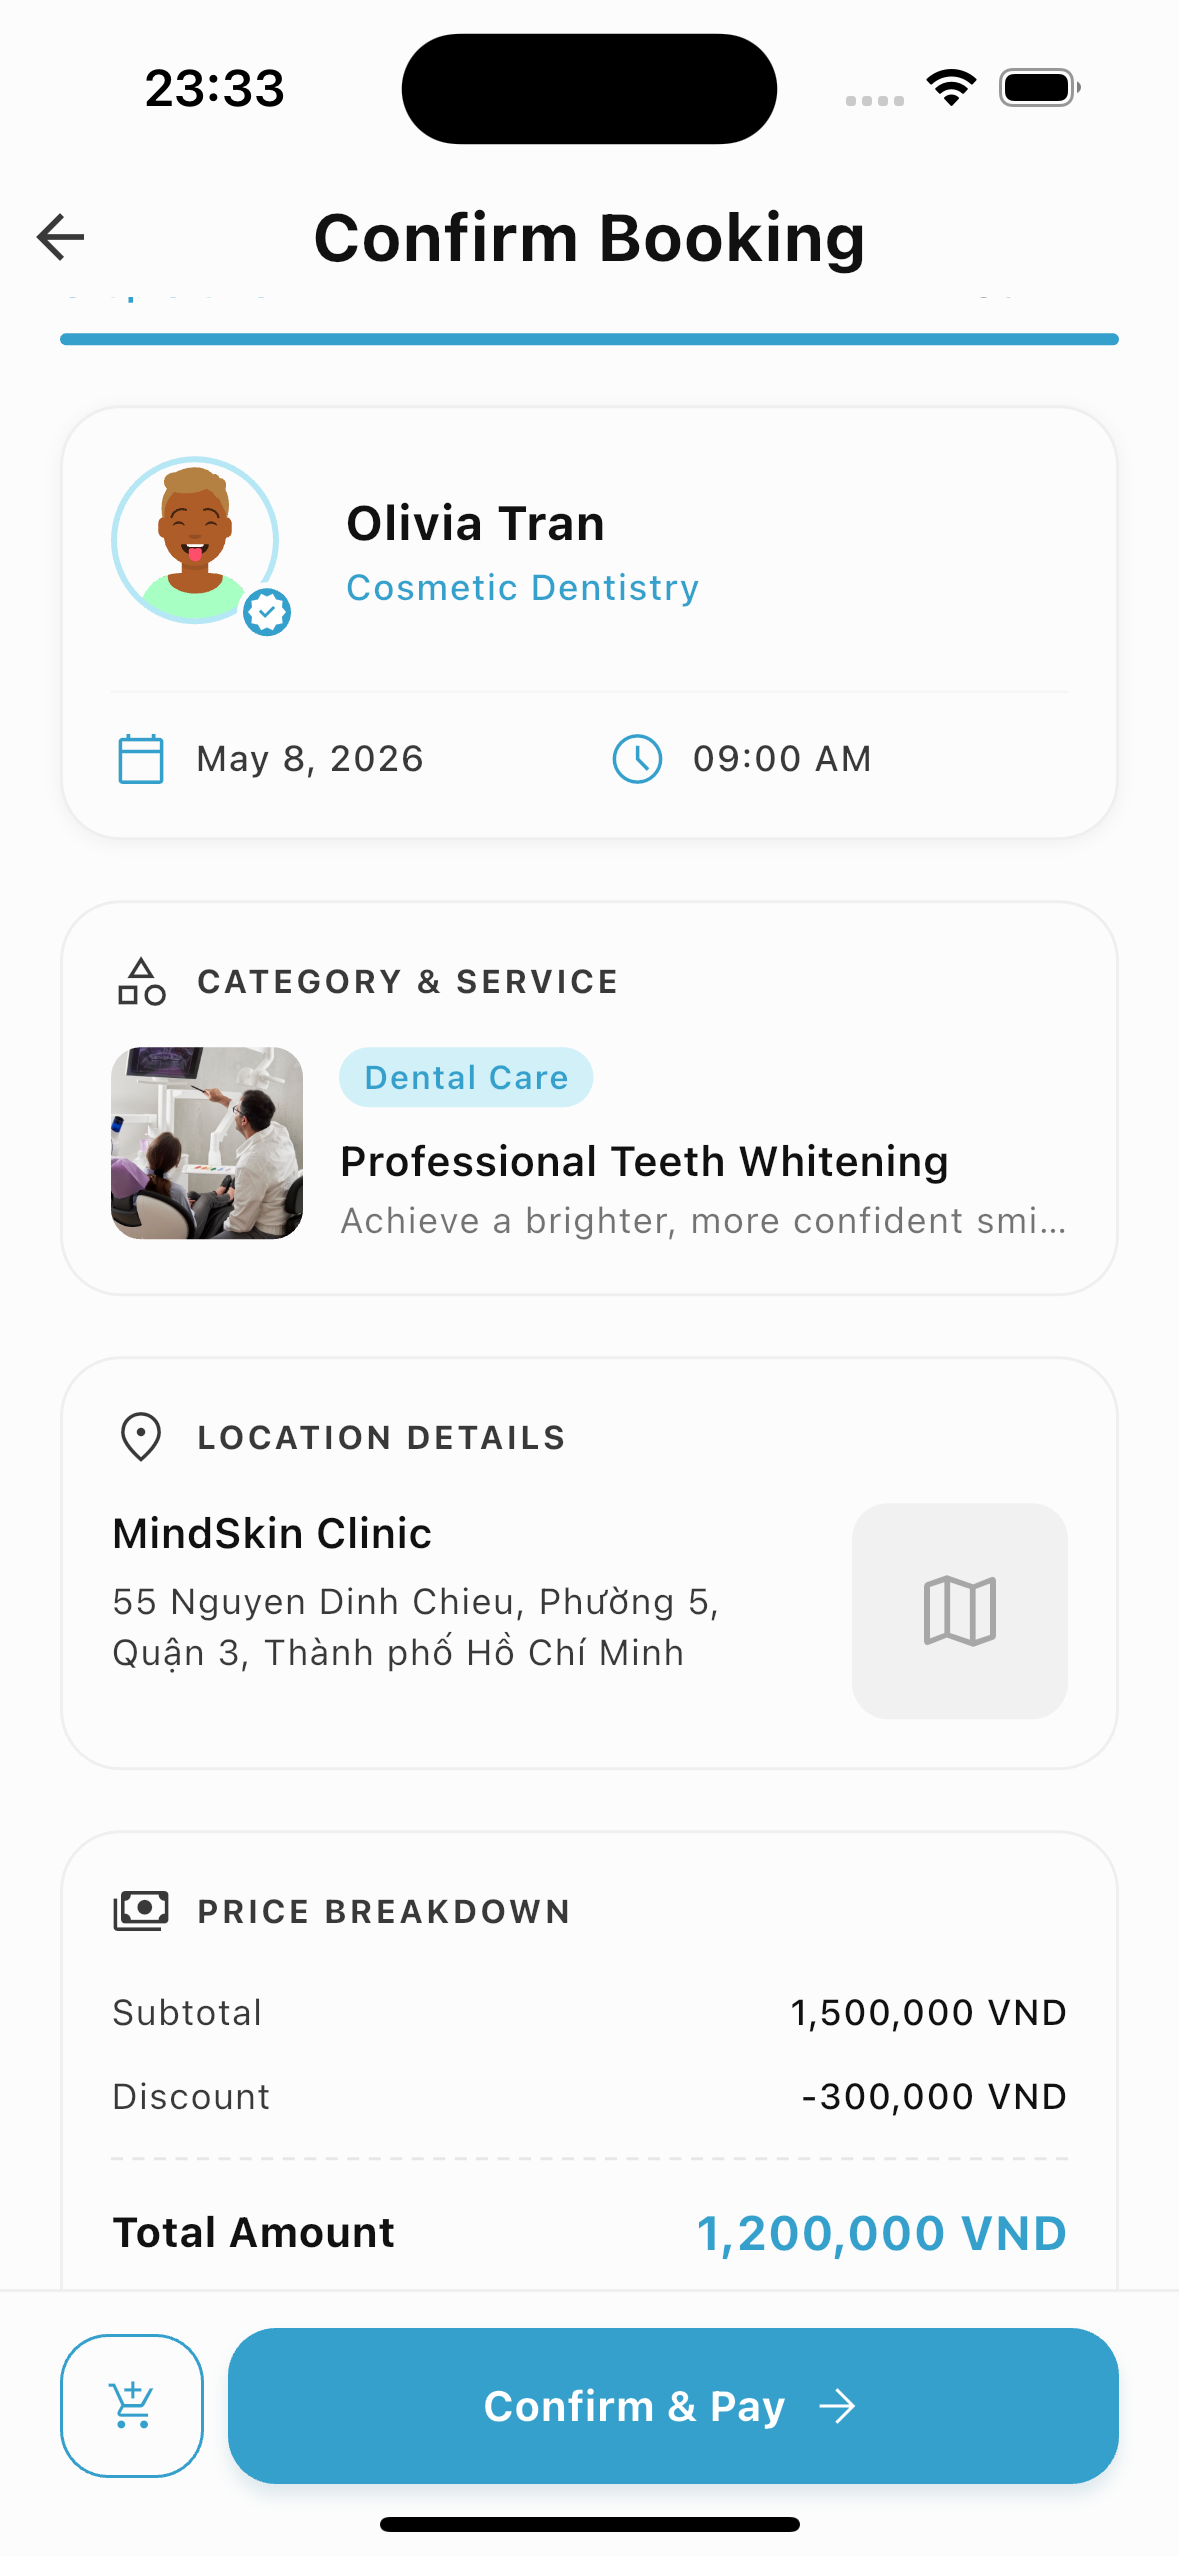
\includegraphics[width=\linewidth,height=0.28\textheight,keepaspectratio]{Images/Hiện thực/user_app/booking/fig_booking_step3_confirm.png}
    \caption{Xác nhận thông tin và bảng giá}
    \label{fig:booking_step3_confirm}
\end{subfigure}
\par\medskip
\caption{Bước 2 \& 3 -- Chọn lịch hẹn và xác nhận đặt lịch}
\label{fig:booking_step2_step3}
\end{figure}

\paragraph{Thanh toán (Checkout \& Payment)}

Sau khi xác nhận đặt lịch, người dùng được chuyển sang màn hình Checkout hiển thị tóm tắt đơn hàng (phòng khám, dịch vụ, chuyên gia, giá) kèm tùy chọn quy đổi xu (Redeem Coins). Hệ thống hỗ trợ ba phương thức thanh toán:

\begin{itemize}
    \item \textbf{Credit/Debit Card:} Thanh toán quốc tế qua cổng Stripe.
    \item \textbf{E-Wallet (MoMo/ZaloPay):} Thanh toán nội địa qua ví điện tử MoMo. Khi chọn phương thức này, ứng dụng mở WebView đến cổng \texttt{test-payment.momo.vn}, hiển thị mã đơn hàng và số tiền để người dùng xác nhận bằng ví MoMo.
    \item \textbf{Pay Later:} Cho phép đặt lịch trước, thanh toán sau tại phòng khám.
\end{itemize}

\begin{figure}[H]
\centering
\captionsetup[subfigure]{font=small,justification=centering}
\captionsetup{skip=8pt}
\begin{subfigure}[t]{0.48\linewidth}
    \centering
    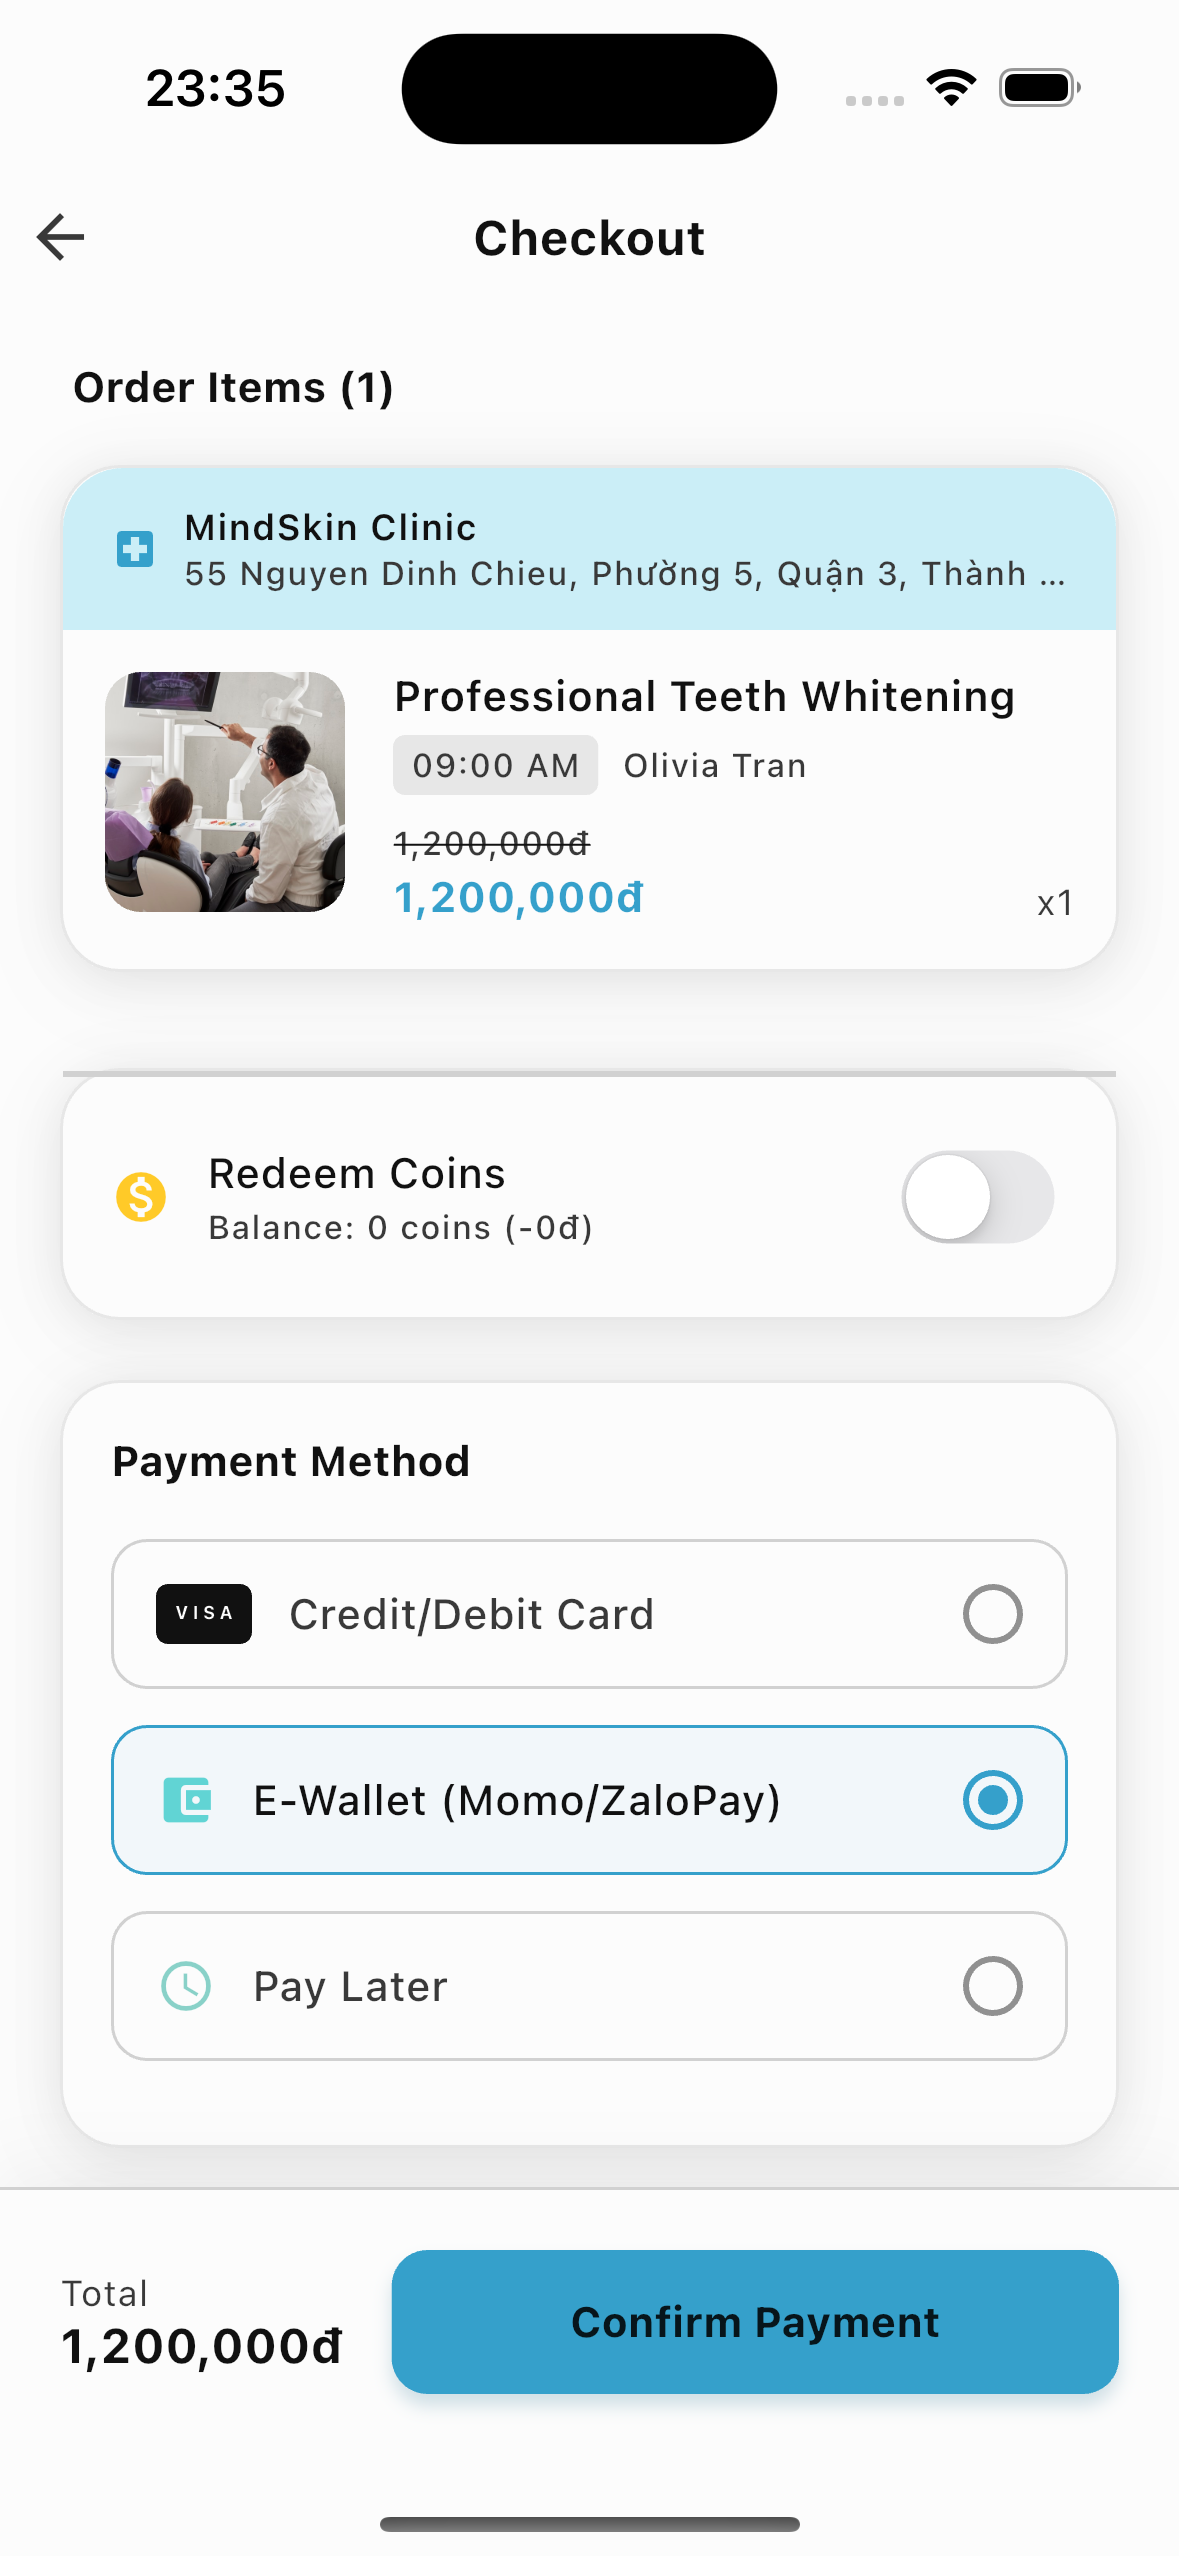
\includegraphics[width=\linewidth,height=0.28\textheight,keepaspectratio]{Images/Hiện thực/user_app/booking/fig_booking_checkout.png}
    \caption{Chọn phương thức thanh toán}
    \label{fig:booking_checkout}
\end{subfigure}
\hfill
\begin{subfigure}[t]{0.48\linewidth}
    \centering
    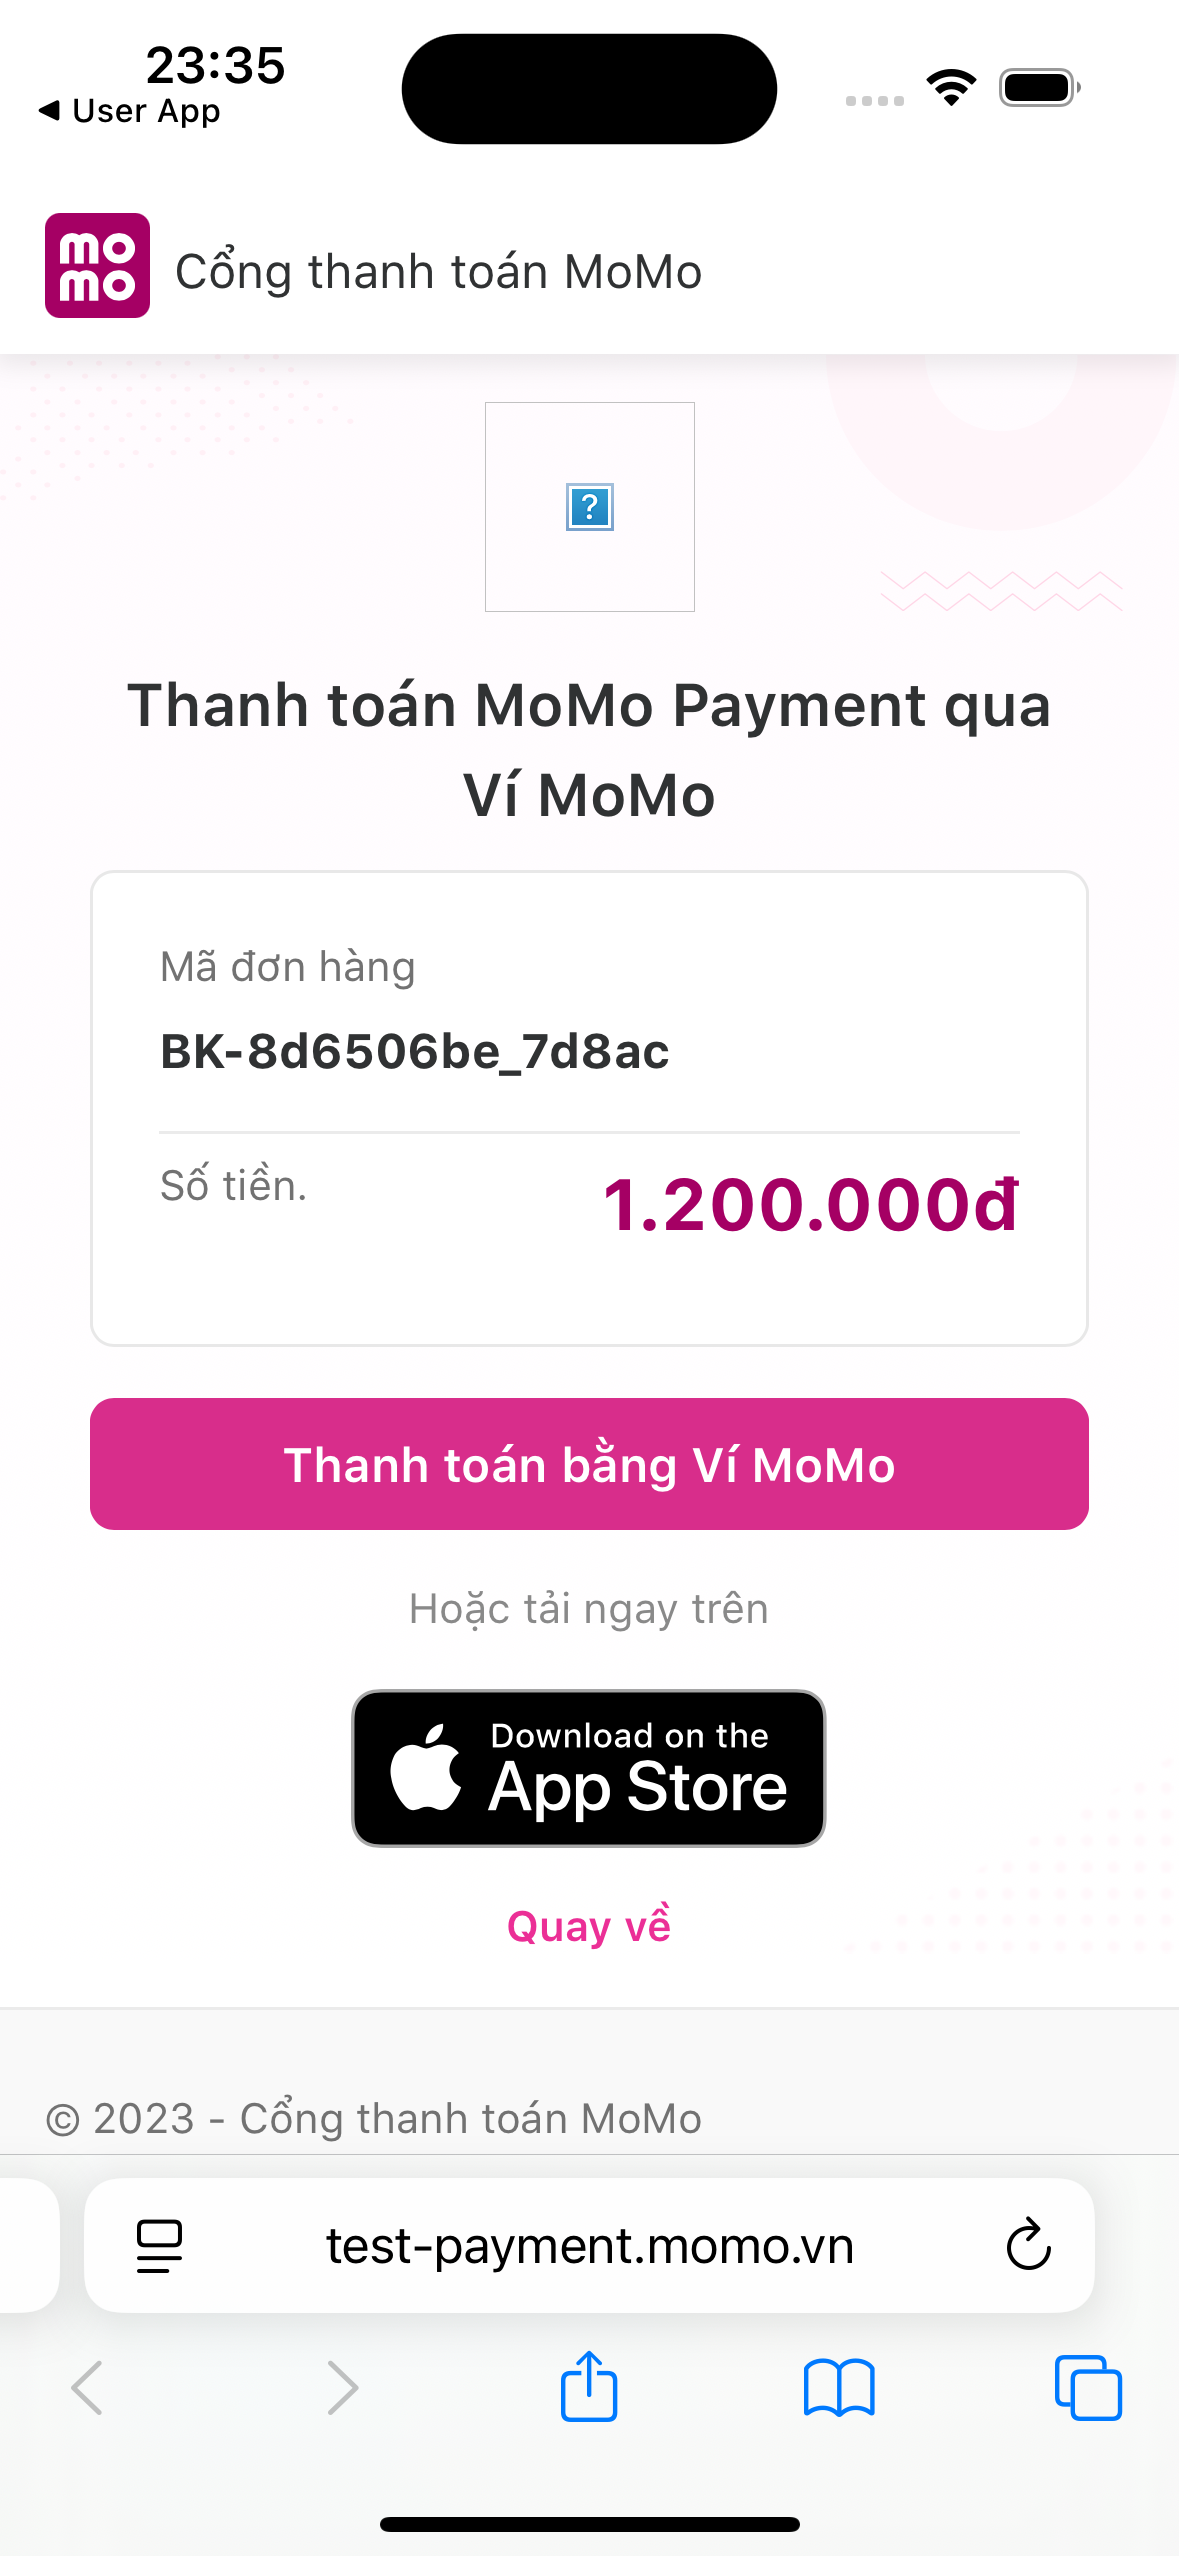
\includegraphics[width=\linewidth,height=0.28\textheight,keepaspectratio]{Images/Hiện thực/user_app/booking/fig_booking_momo_payment.png}
    \caption{Cổng thanh toán MoMo}
    \label{fig:booking_momo_payment}
\end{subfigure}
\par\medskip
\caption{Luồng Checkout và thanh toán qua ví điện tử MoMo}
\label{fig:booking_checkout_flow}
\end{figure}

\textbf{Tính năng kỹ thuật:}

\begin{itemize}
    \item \textbf{Payment Gateway Integration:} Stripe (quốc tế) và MoMo (nội địa), với luồng IPN/Webhook server-to-server xác nhận giao dịch.
    \item \textbf{Redeem Coins:} Người dùng có thể quy đổi xu tích lũy để giảm giá trực tiếp trên tổng đơn hàng.
    \item \textbf{Idempotency:} Sử dụng mã đơn hàng duy nhất (\texttt{BK-*}) ngăn double charge khi retry.
    \item \textbf{Distributed Lock:} Redis Redlock khóa slot trong 10 phút (TTL) từ lúc tạo draft order đến khi thanh toán hoàn tất.
\end{itemize}

\paragraph{Trò chuyện với trợ lý AI (Chat with Dr. AI)}

\begin{figure}[H]
\centering
\begin{subfigure}[b]{0.48\linewidth}
    \centering
    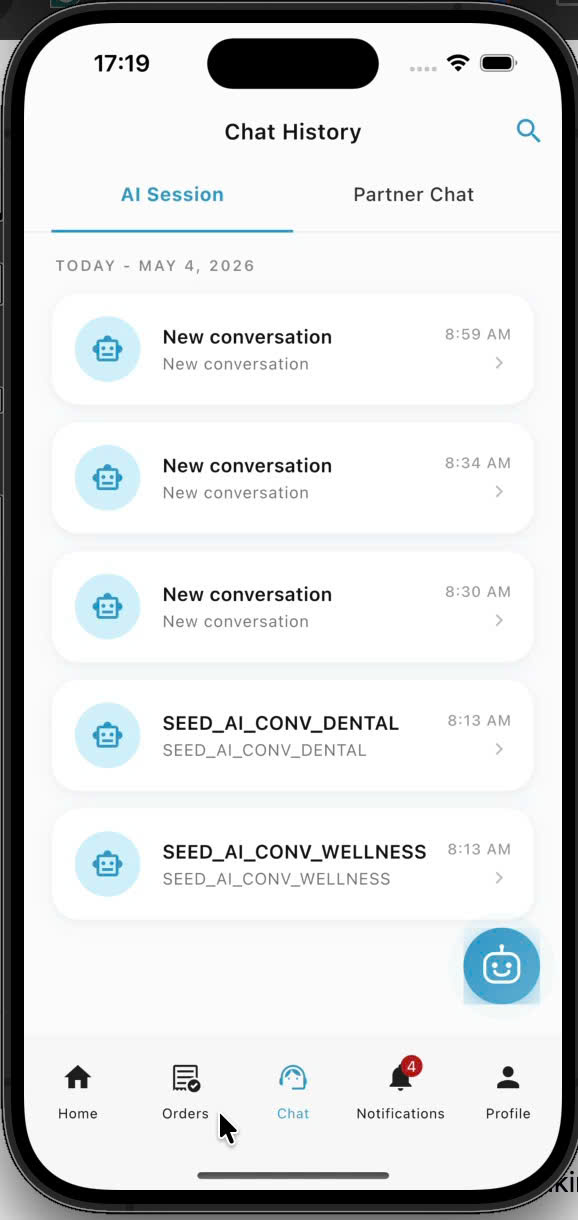
\includegraphics[width=\linewidth,height=0.42\textheight,keepaspectratio,trim=30 40 30 40,clip]{Images/Hiện thực/user/fig_user_chat_history.jpg}
    \caption{Lịch sử chat AI Session (zoom)}
\end{subfigure}
\hfill
\begin{subfigure}[b]{0.48\linewidth}
    \centering
    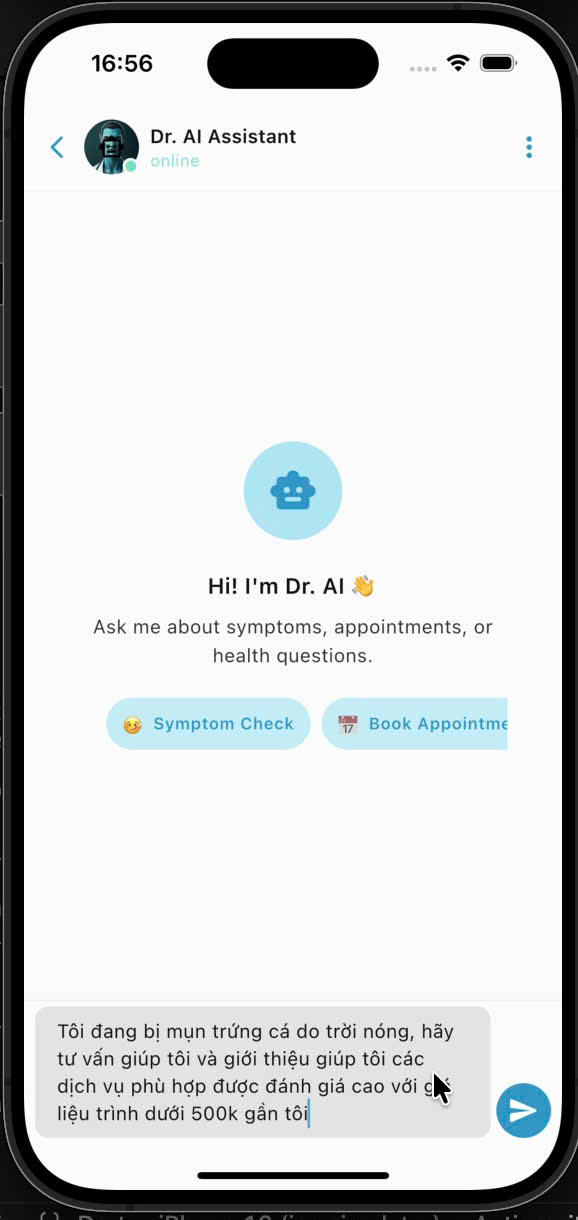
\includegraphics[width=\linewidth,height=0.42\textheight,keepaspectratio,trim=30 40 30 40,clip]{Images/Hiện thực/user/fig_user_chat_ask_2.jpg}
    \caption{Cuộc trò chuyện chi tiết (zoom)}
\end{subfigure}
\par\medskip
\caption{Màn hình Chat History - Tư vấn AI}
\label{fig:user_chat_history}
\end{figure}

\begin{itemize}
    \item \textbf{Thao tác mở hội thoại:} Người dùng chọn một phiên chat trong \textit{AI Session} để xem lịch sử chi tiết.
    \item \textbf{Thao tác gửi câu hỏi:} Nhập nội dung ở ô tin nhắn và nhấn nút gửi để nhận phản hồi từ Dr. AI.
\end{itemize}

\textbf{Tính năng kỹ thuật:}

\begin{itemize}
    \item \textbf{LLM Integration:} Chat AI dùng GPT-4 hoặc Llama.
    \item \textbf{Streaming Response:} Stream từng token qua SSE/WebSocket.
    \item \textbf{Context Preservation:} Lưu context trên server.
    \item \textbf{Service Recommendation:} Gợi ý dịch vụ phù hợp.
\end{itemize}

\paragraph{Chi tiết dịch vụ (Service Detail)}

\begin{figure}[H]
\centering
\captionsetup[subfigure]{font=small,justification=centering}
\captionsetup{skip=6pt}
\begin{subfigure}[t]{0.48\linewidth}
    \centering
    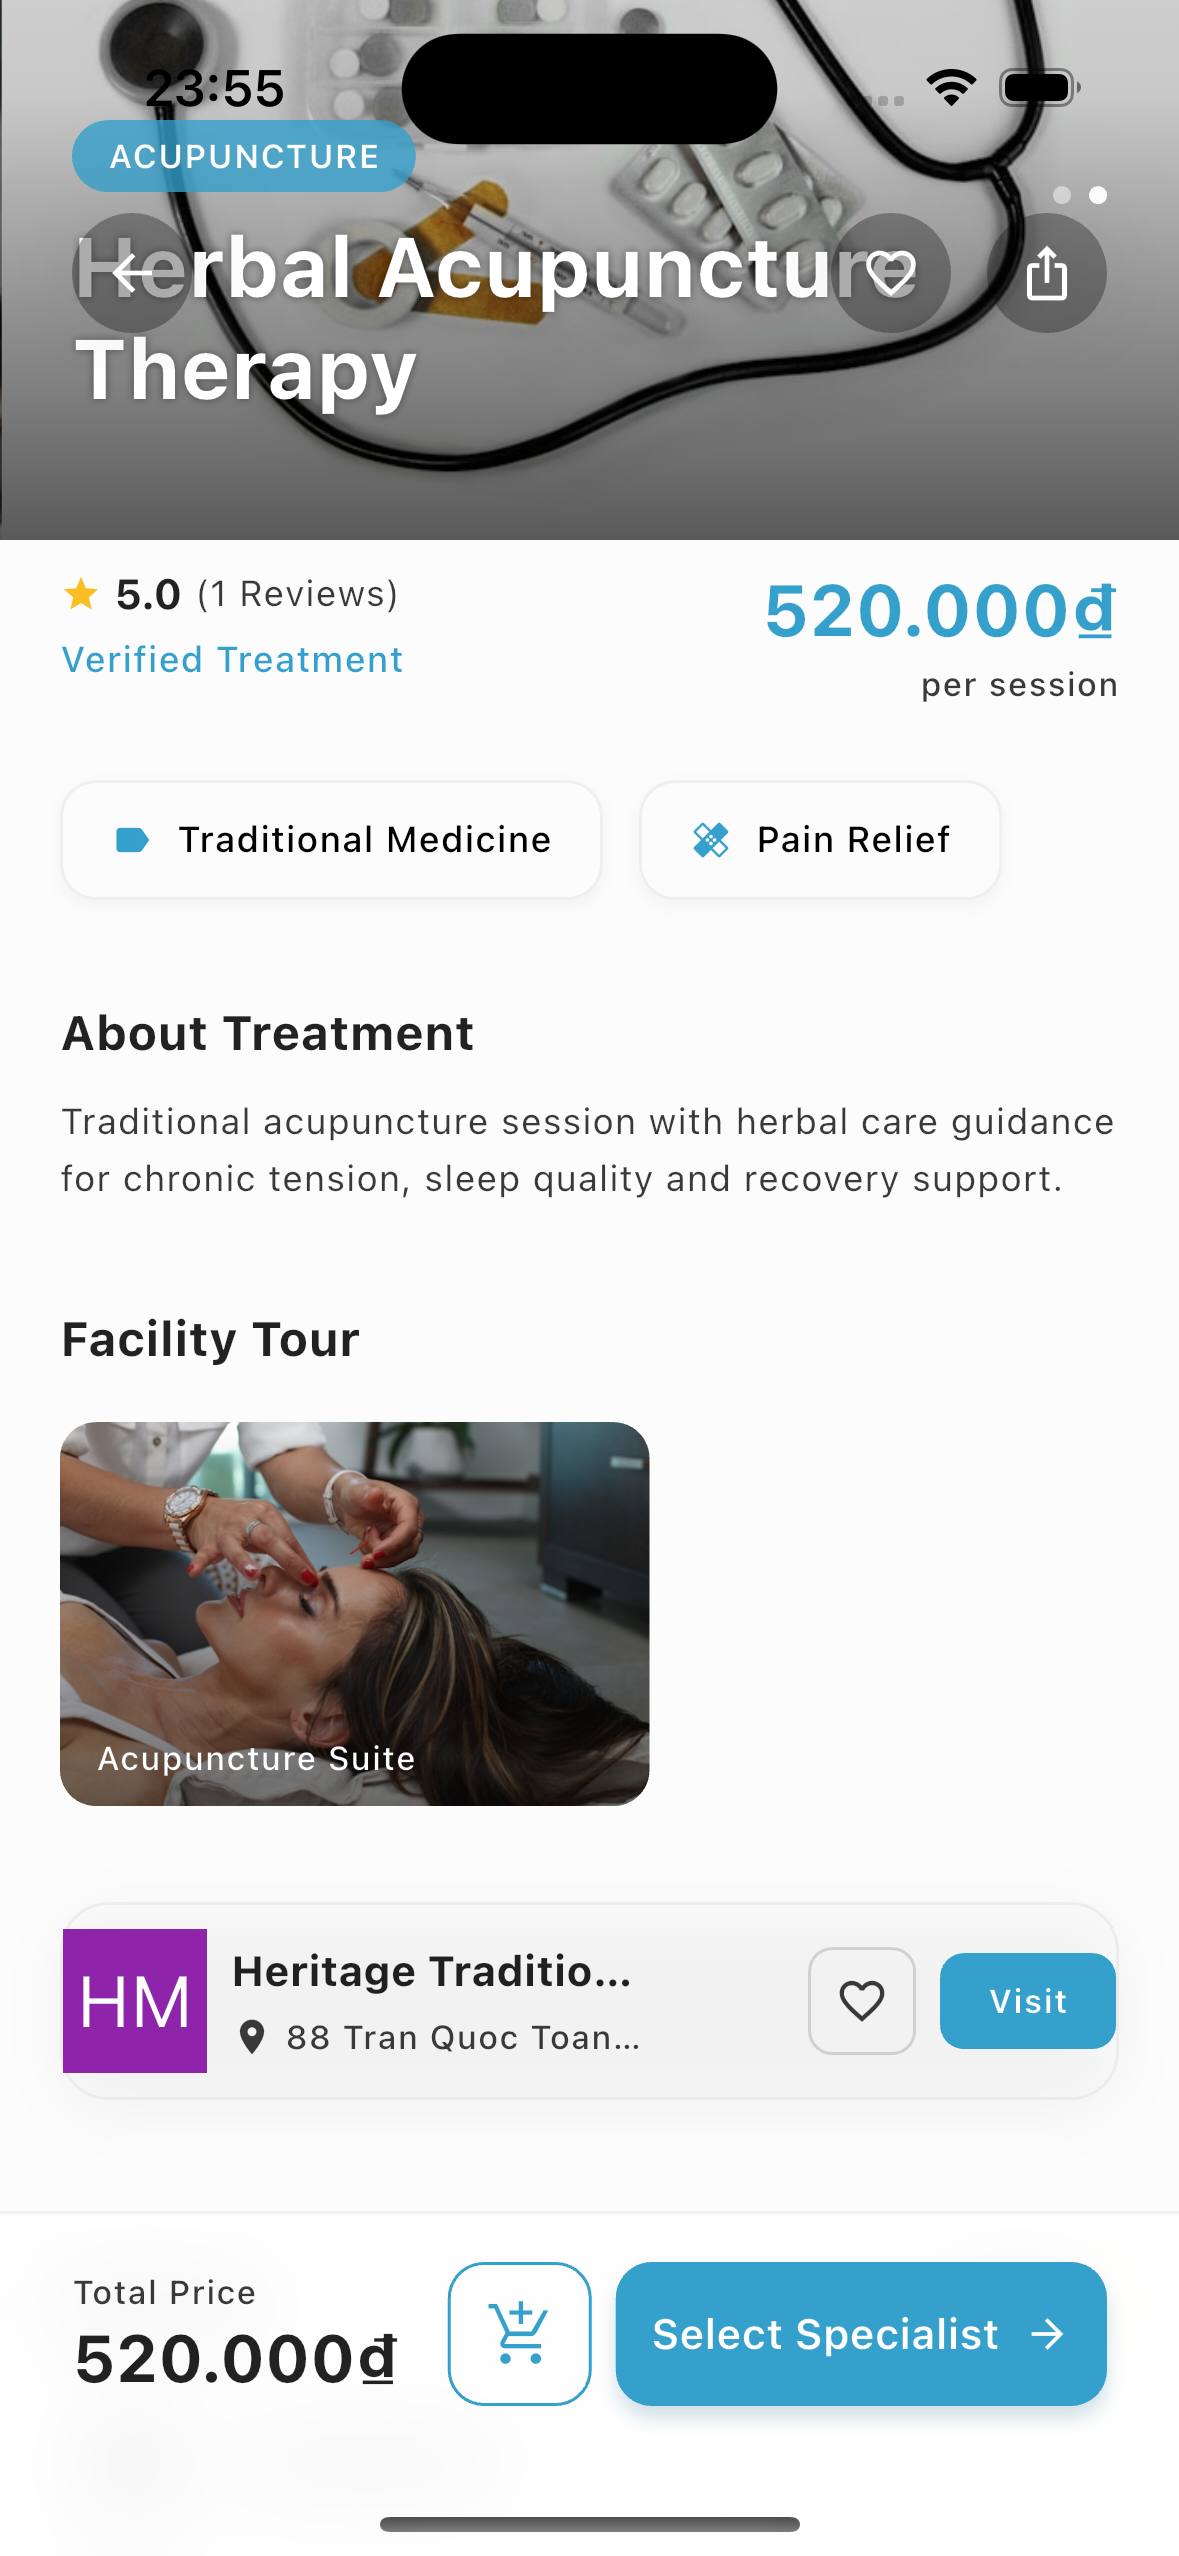
\includegraphics[width=\linewidth,height=0.4\textheight,keepaspectratio]{Images/Hiện thực/user_app/service_details/Simulator Screenshot - iPhone 16 - 2026-05-07 at 23.55.30.png}
    \caption{Tổng quan dịch vụ}
    \label{fig:service_detail_overview}
\end{subfigure}
\hfill
\begin{subfigure}[t]{0.48\linewidth}
    \centering
    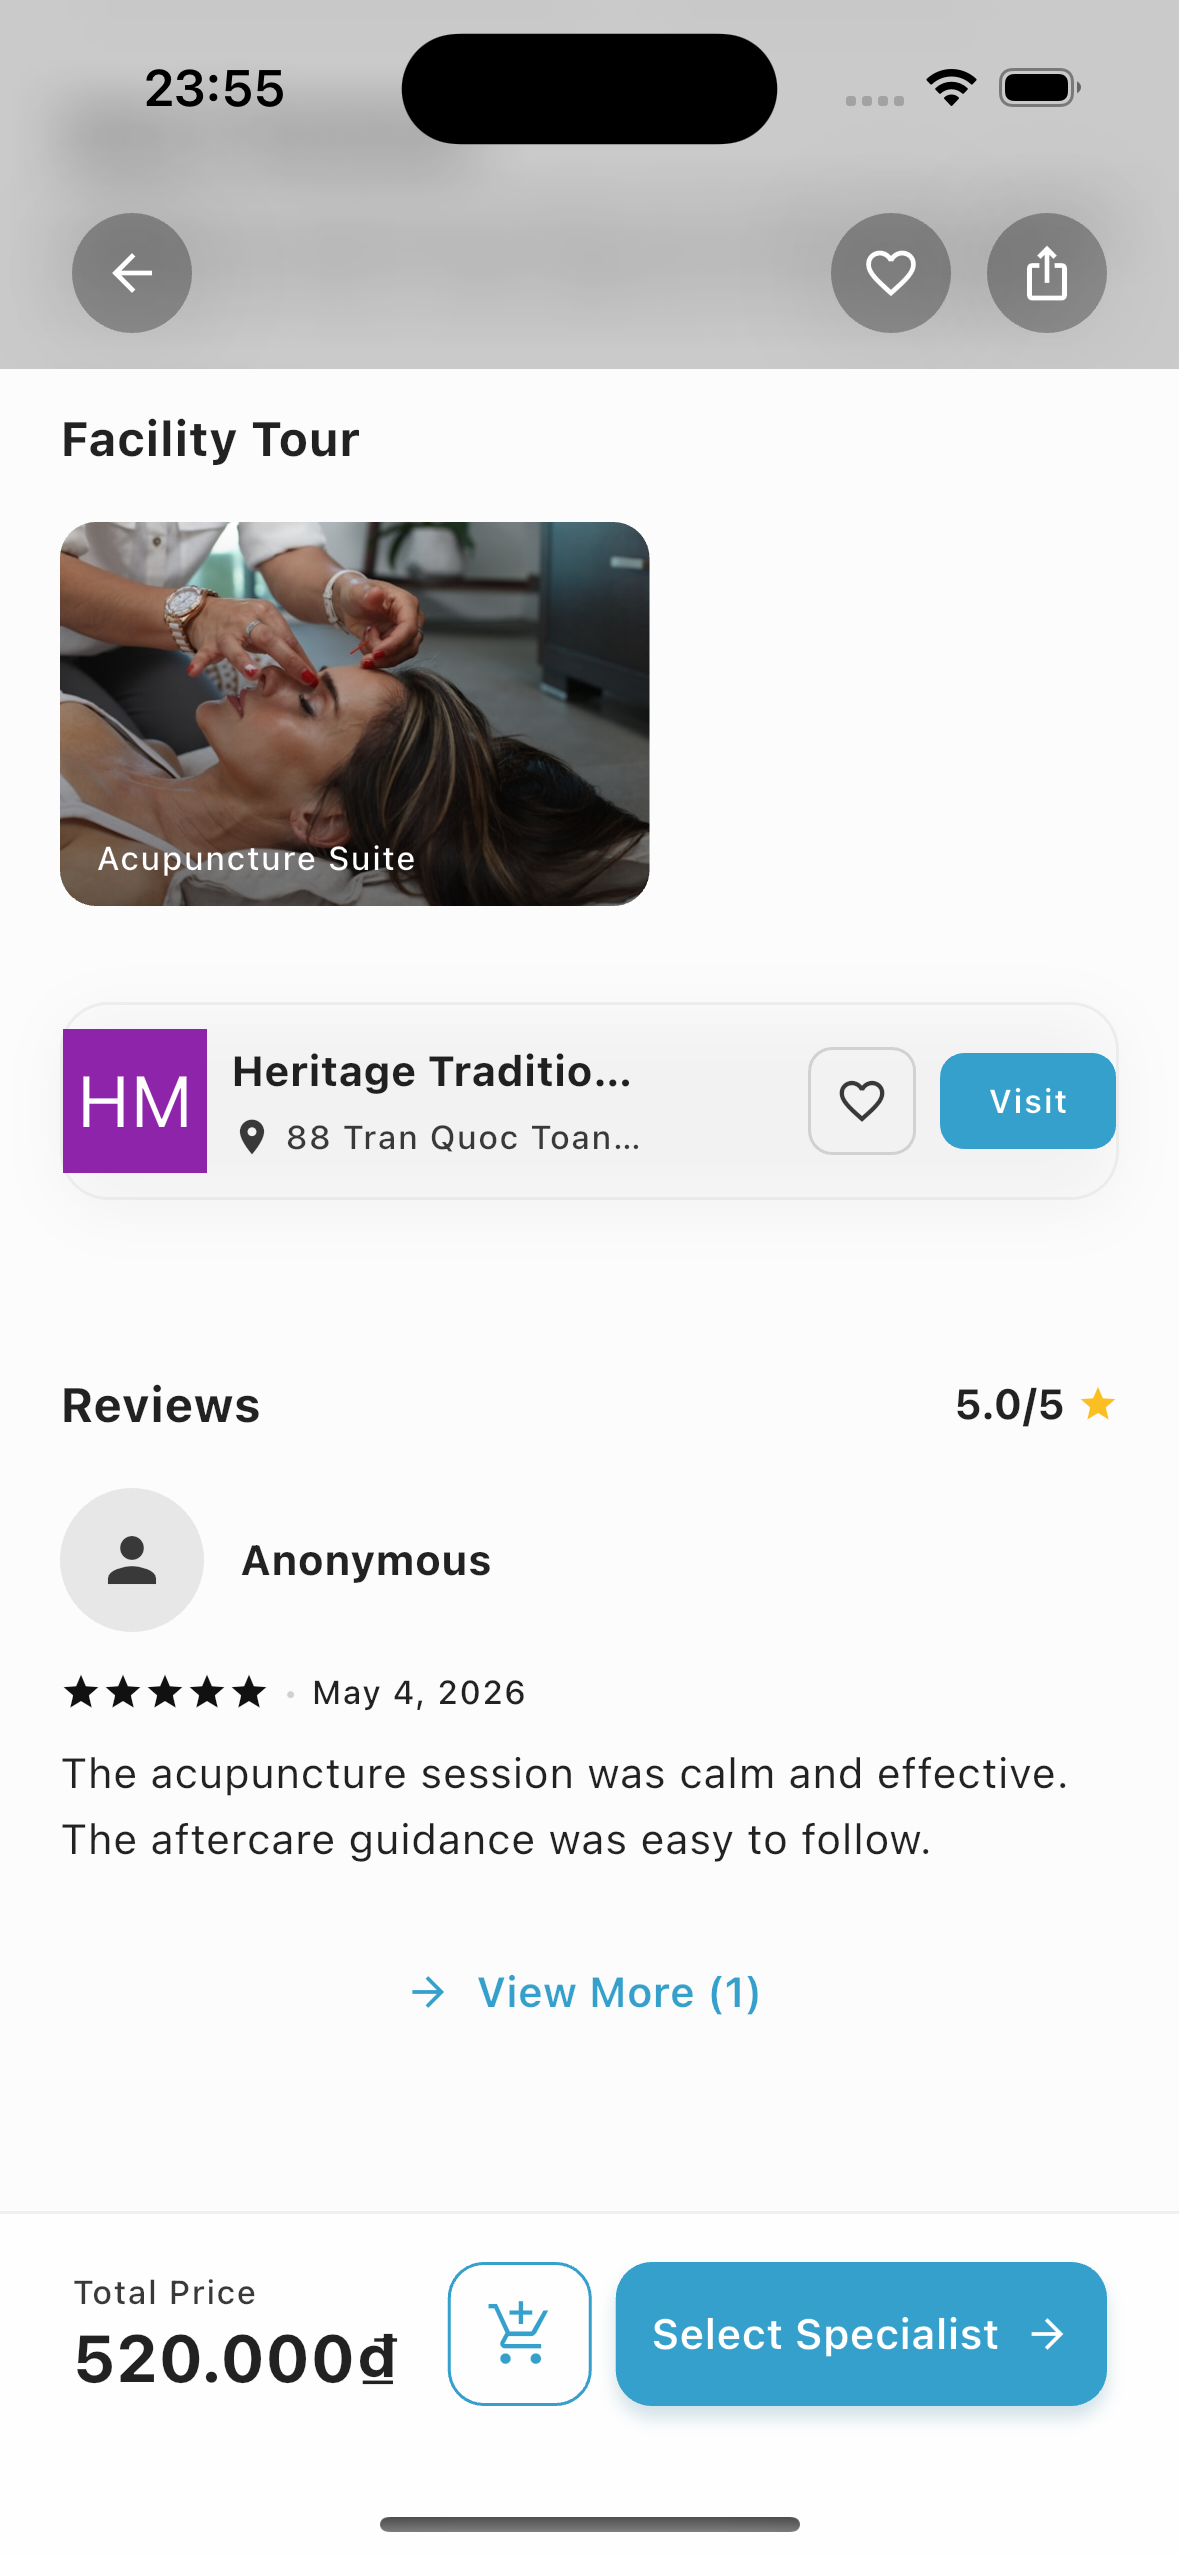
\includegraphics[width=\linewidth,height=0.4\textheight,keepaspectratio]{Images/Hiện thực/user_app/service_details/Simulator Screenshot - iPhone 16 - 2026-05-07 at 23.55.38.png}
    \caption{Phần đánh giá và nhận xét}
    \label{fig:service_detail_reviews}
\end{subfigure}
\par\medskip
\caption{Luồng Service Detail trên ứng dụng người dùng}
\label{fig:user_service_detail_flow}
\end{figure}

\begin{figure}[H]
\centering
\captionsetup[subfigure]{font=small,justification=centering}
\captionsetup{skip=8pt}
\begin{subfigure}[t]{0.48\linewidth}
    \centering
    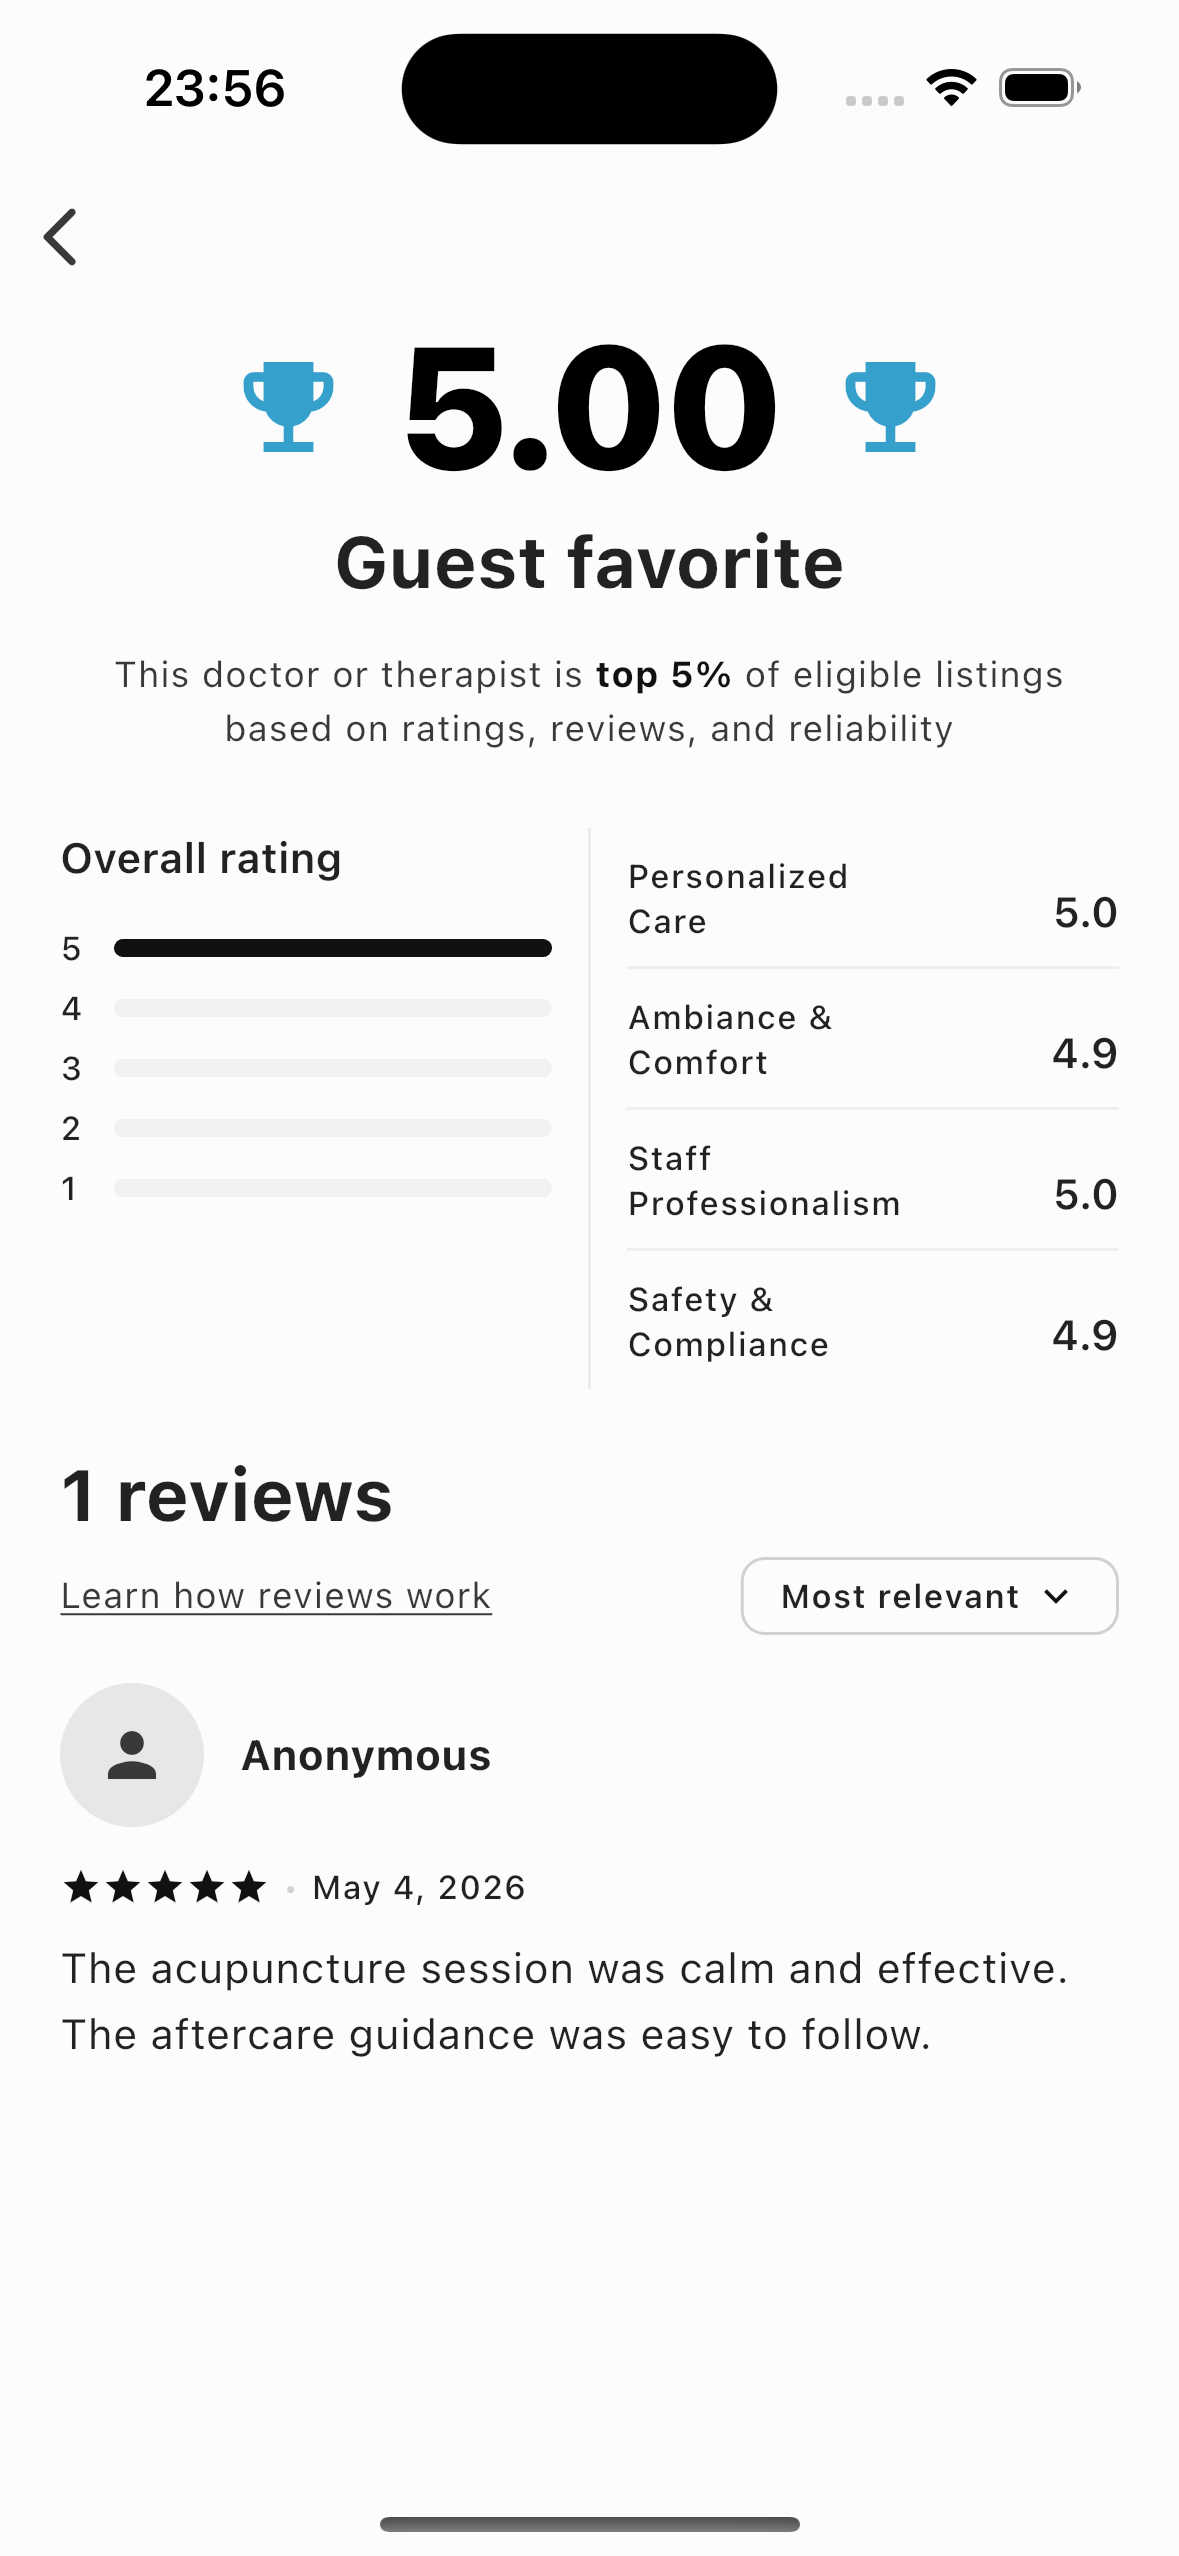
\includegraphics[width=\linewidth,height=0.4\textheight,keepaspectratio]{Images/Hiện thực/user_app/service_details/Simulator Screenshot - iPhone 16 - 2026-05-07 at 23.56.00.png}
    \caption{Bảng xếp hạng chi tiết}
    \label{fig:service_detail_ratings}
\end{subfigure}
\hfill
\begin{subfigure}[t]{0.48\linewidth}
    \centering
    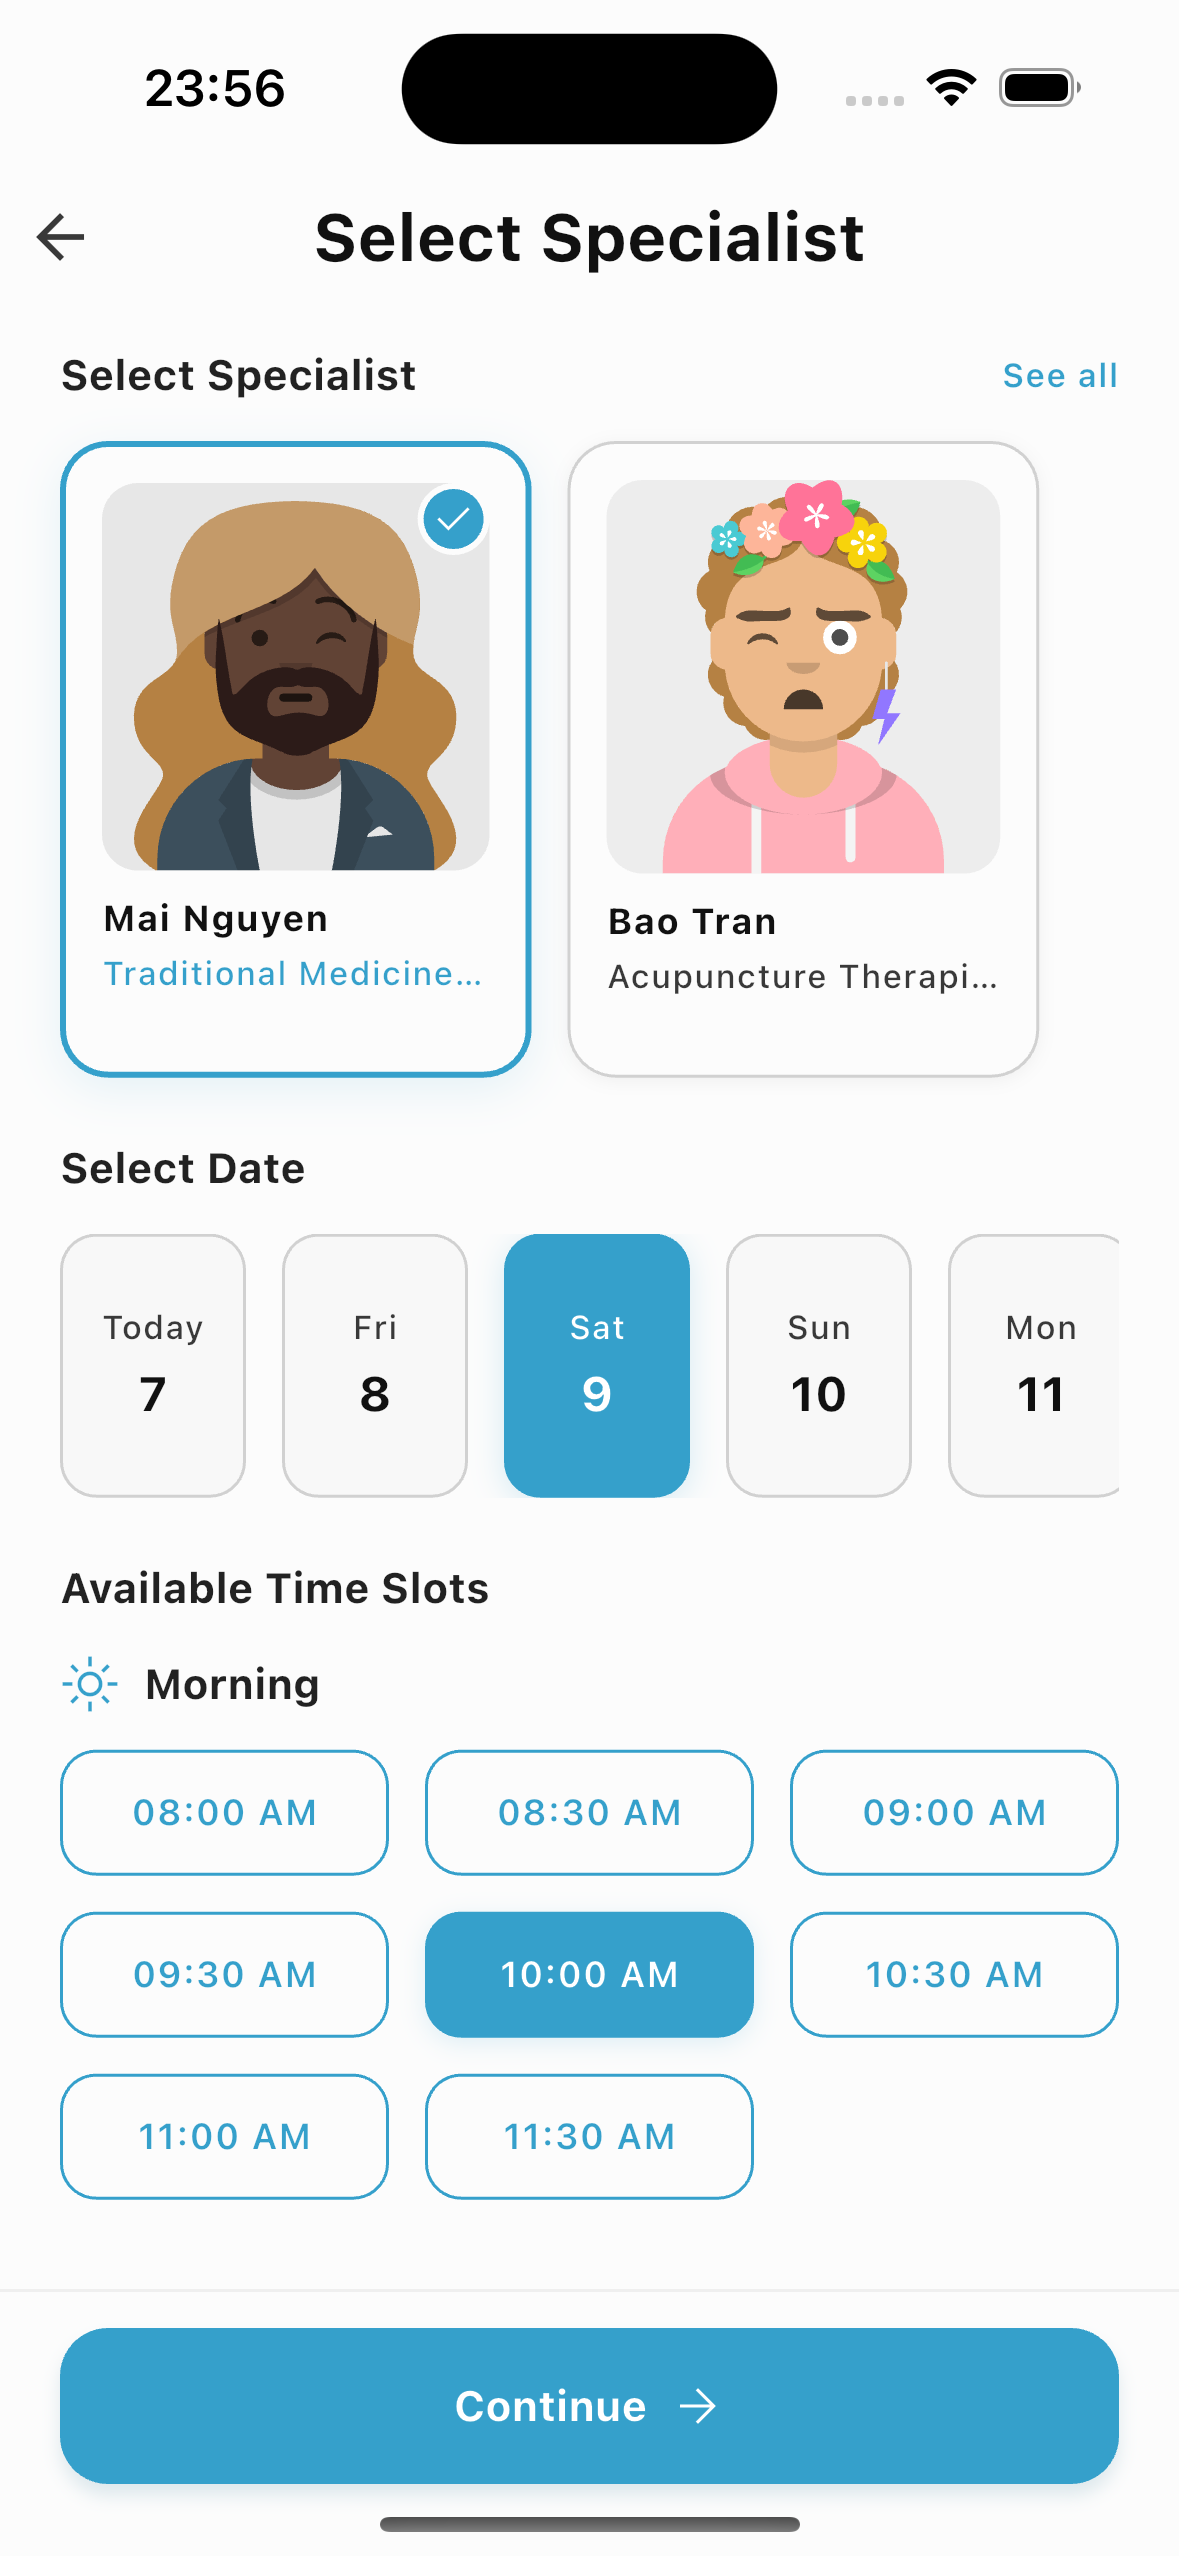
\includegraphics[width=\linewidth,height=0.4\textheight,keepaspectratio]{Images/Hiện thực/user_app/service_details/Simulator Screenshot - iPhone 16 - 2026-05-07 at 23.56.18.png}
    \caption{Chọn chuyên gia và khung giờ}
    \label{fig:service_detail_select_specialist}
\end{subfigure}
\par\medskip
\begin{subfigure}[t]{0.48\linewidth}
    \centering
    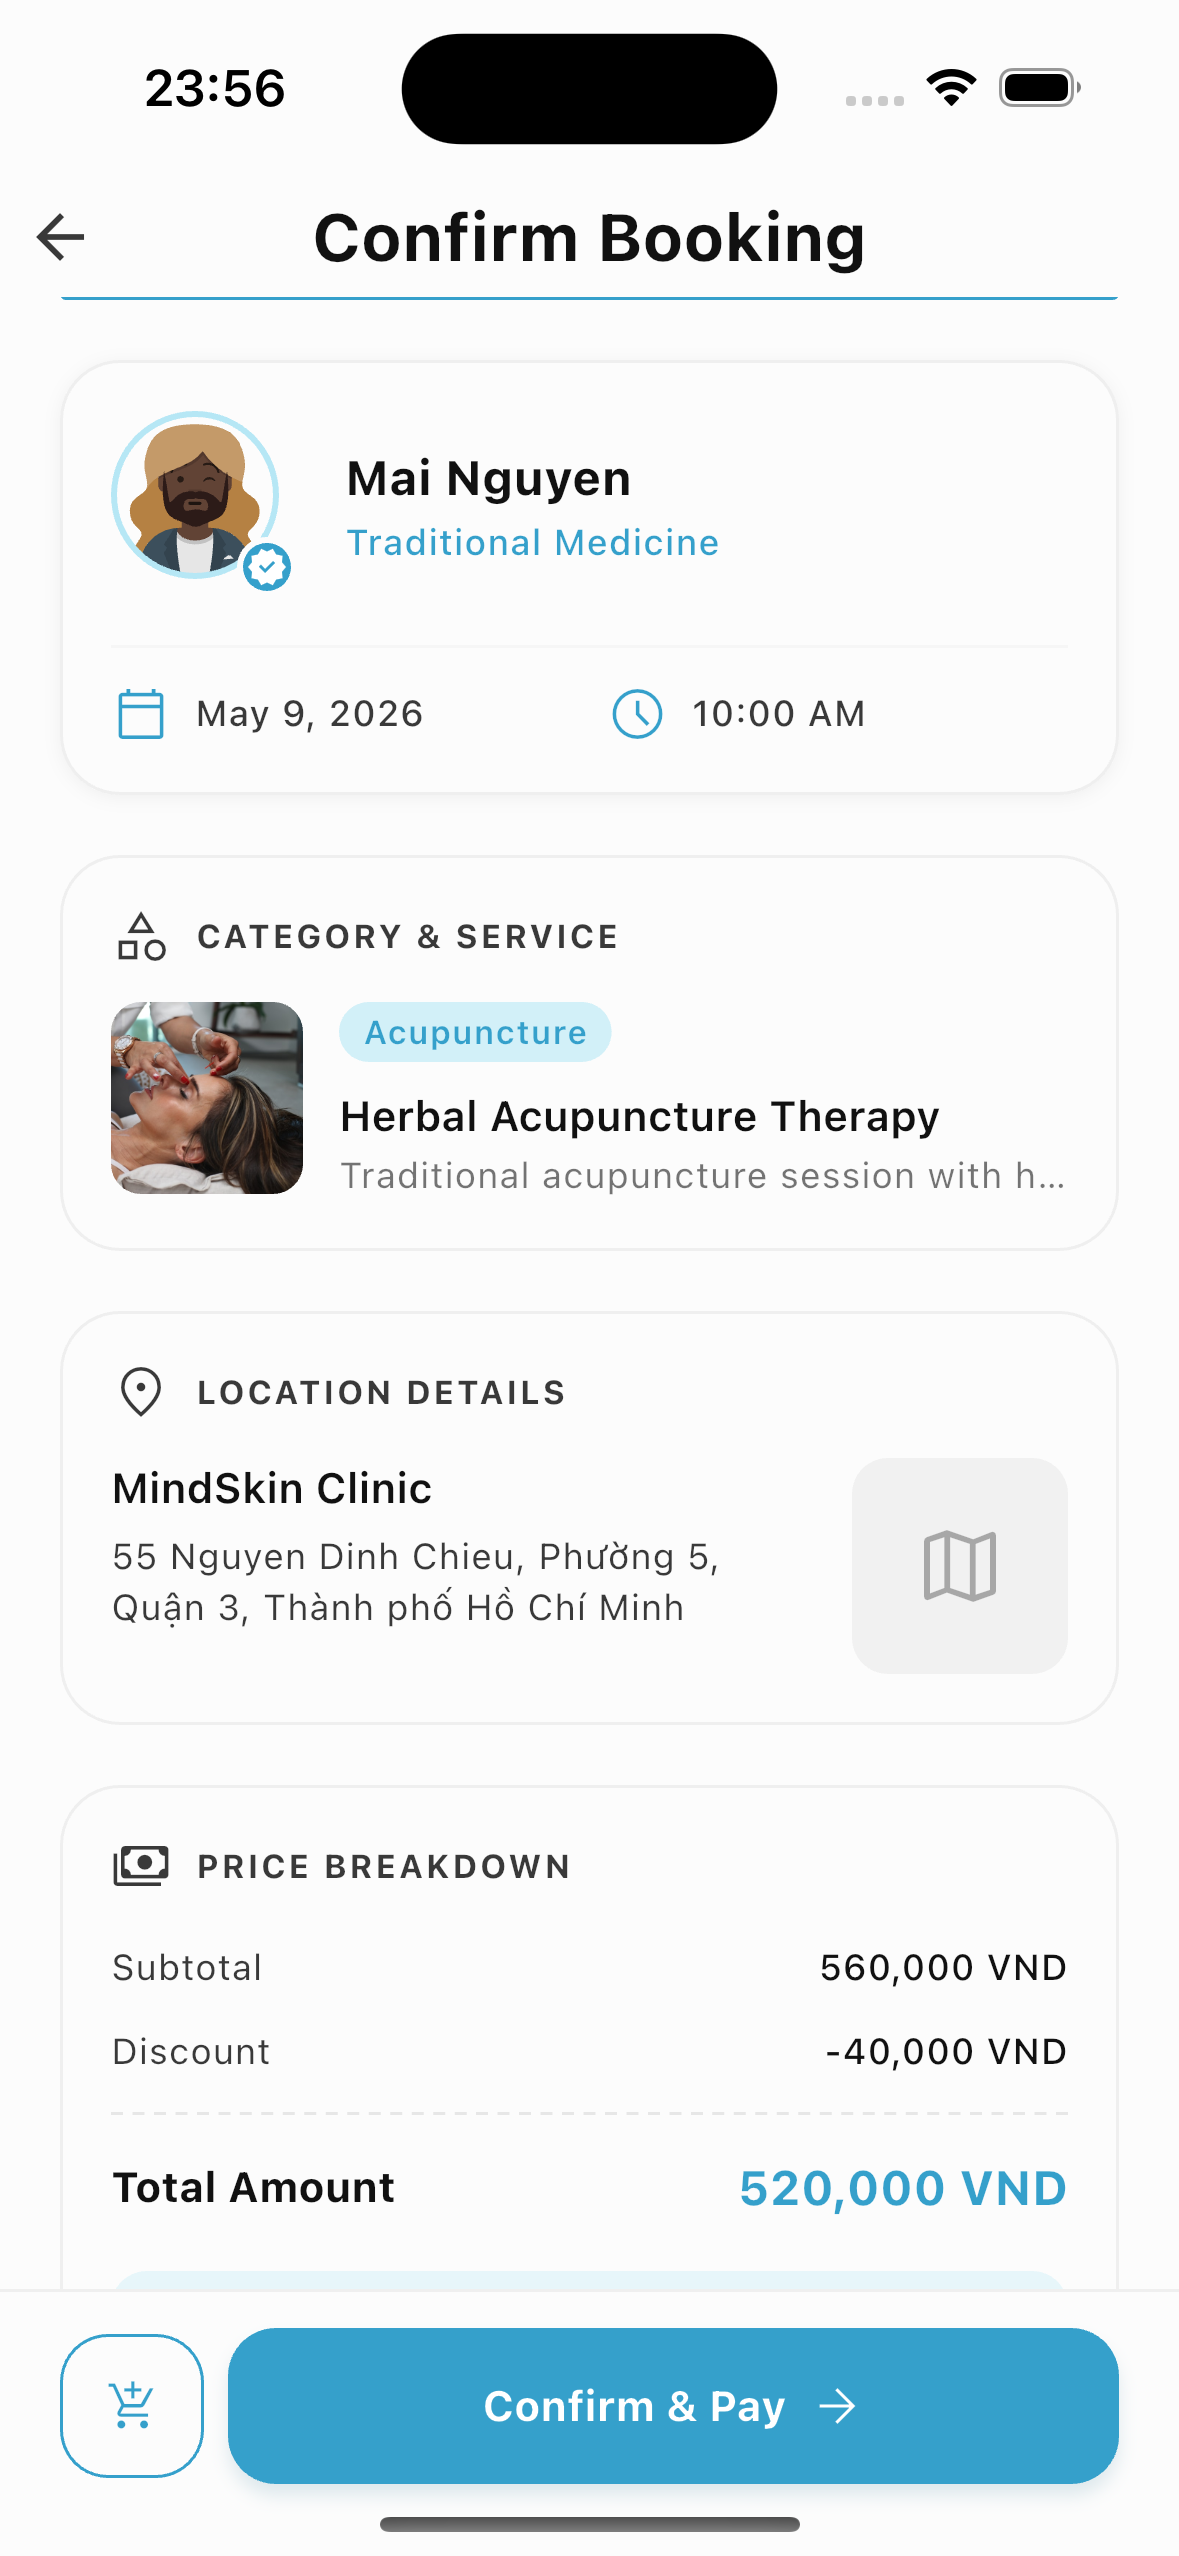
\includegraphics[width=\linewidth,height=0.4\textheight,keepaspectratio]{Images/Hiện thực/user_app/service_details/Simulator Screenshot - iPhone 16 - 2026-05-07 at 23.56.31.png}
    \caption{Xác nhận đặt lịch}
    \label{fig:service_detail_confirm}
\end{subfigure}
\par\medskip
\caption{Luồng đặt lịch dịch vụ trên ứng dụng người dùng}
\label{fig:user_service_booking_flow}
\end{figure}

\begin{itemize}
    \item \textbf{Thao tác xem thông tin:} Người dùng xem ảnh bìa, nhãn dịch vụ, giá, mô tả ngắn và các đánh giá để đánh giá nhanh chất lượng dịch vụ.
    \item \textbf{Thao tác đặt lịch:} Người dùng kéo xuống phần đánh giá, chọn chuyên gia, chọn ngày giờ phù hợp rồi chuyển sang màn hình xác nhận đặt lịch.
\end{itemize}

\subsubsection{Kiến trúc dữ liệu và API}

\paragraph{API Endpoints chính}

\begin{table}[H]
\centering
\begin{tabularx}{\linewidth}{|l|X|X|}
\hline
\textbf{Endpoint} & \textbf{Phương thức} & \textbf{Mô tả} \\
\hline
\texttt{/v1/services} & GET & Lấy danh sách dịch vụ \\
\hline
\texttt{/v1/appointments} & GET & Danh sách lịch hẹn \\
\hline
\texttt{/v1/appointments} & POST & Tạo lịch hẹn mới \\
\hline
\texttt{/v1/payments} & POST & Khởi tạo thanh toán \\
\hline
\texttt{/v1/ai/chat} & POST & Chat với AI \\
\hline
\end{tabularx}
\caption{Danh sách API endpoints chính}
\label{tab:user_api_endpoints}
\end{table}

\subsubsection{Quy trình xử lý nghiệp vụ}

\paragraph{Quy trình đặt lịch hẹn}

\begin{enumerate}
    \item Người dùng chọn dịch vụ
    \item Backend lấy slot khả dụng từ lịch làm việc chuyên gia
    \item Sử dụng Redis Redlock ngăn chặn race condition
    \item Tạo draft order với TTL 10 phút
    \item Thanh toán và xác nhận appointment
\end{enumerate}

\subsubsection{Tối ưu hóa hiệu năng}

\begin{itemize}
    \item \textbf{Caching:} Service cache 24 giờ, User cache 1 giờ
    \item \textbf{CDN:} Hình ảnh trên CloudFront/Cloudflare
    \item \textbf{Image Compression:} 80\% quality, 300-500KB per image
    \item \textbf{Lazy Loading:} Render khi scroll tới
    \item \textbf{Code Splitting:} Lazy-load screens không cần thiết
\end{itemize}


% ===========================================================================
% 6.3.3  PHÂN HỆ CỔNG ĐỐI TÁC (PARTNER PORTAL)
% ===========================================================================
\subsection{Hiện thực Phân hệ Cổng Đối tác (Partner Portal)}

Phân hệ Cổng Đối tác hỗ trợ nhà cung cấp quản lý toàn bộ vòng đời vận hành: từ đăng ký và xét duyệt hồ sơ pháp lý, hoàn thiện hồ sơ công khai, quản trị dịch vụ và nhân sự, đến xử lý lịch hẹn và theo dõi chỉ số kinh doanh.

\paragraph{Xử lý phía Backend khi đăng ký}

Khi đối tác nhấn \textbf{``Complete Registration''}, hệ thống thực hiện các bước sau trong cùng một giao dịch (transaction) để đảm bảo tính toàn vẹn dữ liệu:

\begin{enumerate}
    \item \textbf{Kiểm tra trùng lặp:} Đảm bảo email và mã số thuế chưa có trong hệ thống.
    \item \textbf{Kiểm tra địa chỉ:} Xác nhận thông tin tỉnh/huyện/xã hợp lệ thông qua \texttt{LocationsService}.
    \item \textbf{Khởi tạo dữ liệu:} Khởi tạo thông tin tài khoản, thông tin doanh nghiệp, người đại diện pháp lý, và các giấy tờ KYC ban đầu.
    \item \textbf{Cấp quyền truy cập:} Tạo token truy cập để đối tác có thể đăng nhập ngay.
\end{enumerate}

\begin{figure}[H]
\centering
\begin{subfigure}[b]{0.48\linewidth}
    \centering
    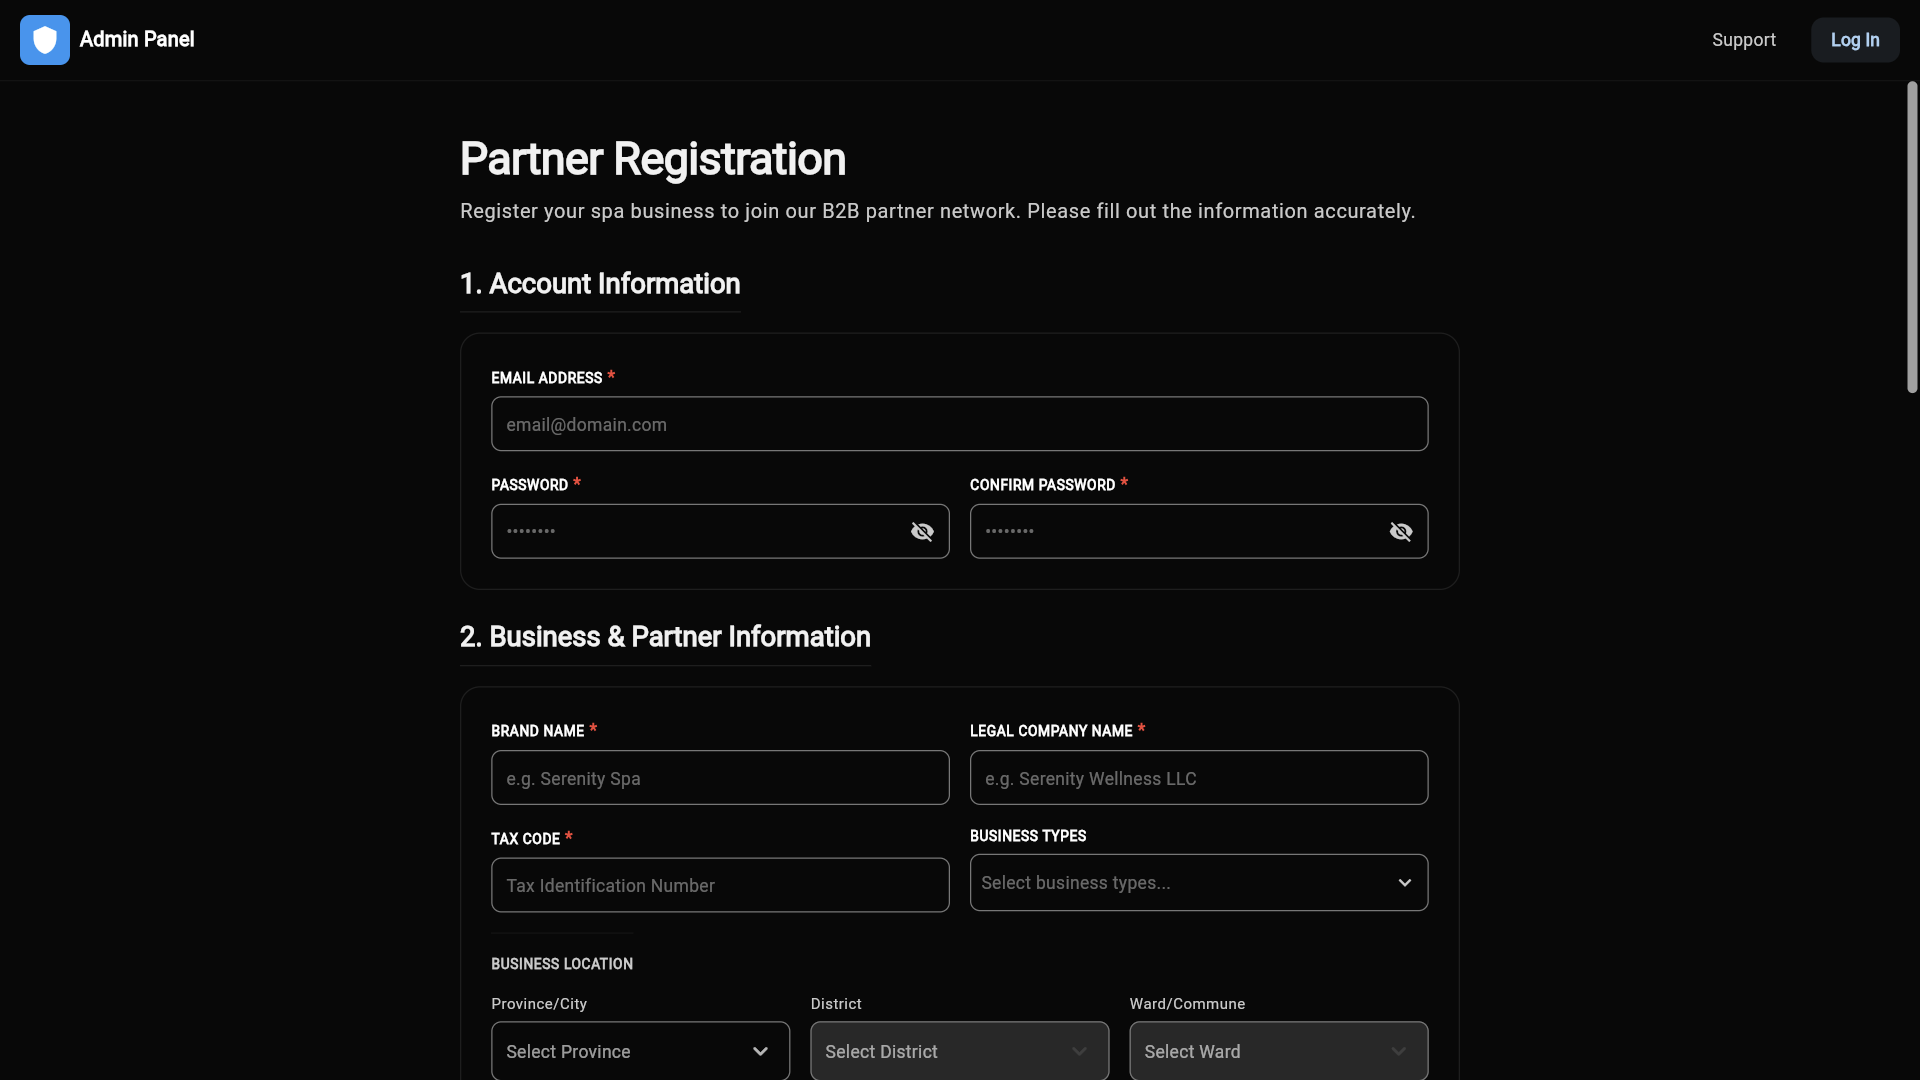
\includegraphics[width=\linewidth]{Images/Hiện thực/partner/fig_partner_reg_account.png}
    \caption{Bước tạo tài khoản đối tác}
    \label{fig:partner_reg_account}
\end{subfigure}
\hfill
\begin{subfigure}[b]{0.48\linewidth}
    \centering
    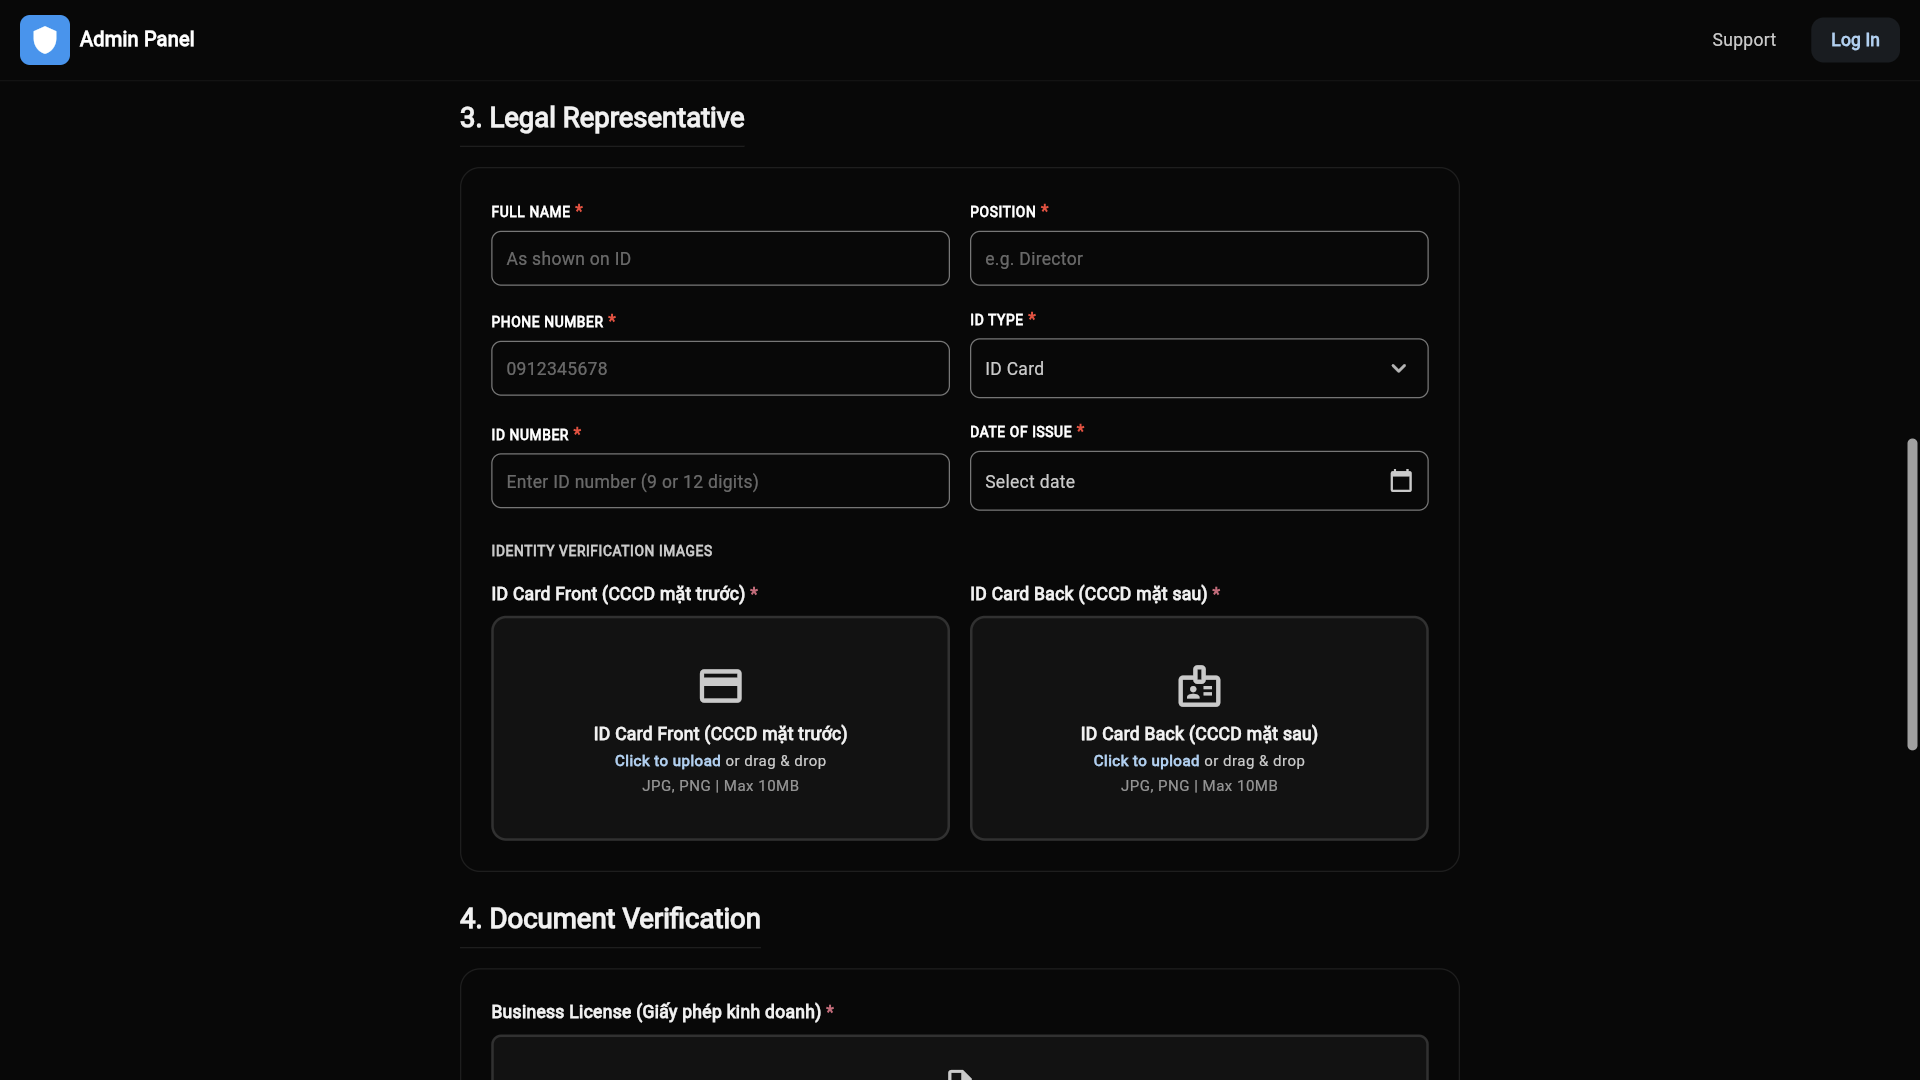
\includegraphics[width=\linewidth]{Images/Hiện thực/partner/fig_partner_reg_legal.png}
    \caption{Khai báo đại diện pháp lý}
    \label{fig:partner_reg_legal}
\end{subfigure}
\par\medskip
\caption{Luồng đăng ký đối tác -- giai đoạn tài khoản và pháp lý}
\end{figure}

\begin{itemize}
    \item \textbf{Thao tác tạo tài khoản:} Đối tác nhập thông tin đăng nhập và dữ liệu liên hệ cơ bản.
    \item \textbf{Thao tác khai báo pháp lý:} Đối tác điền thông tin đại diện pháp luật và giấy tờ định danh bắt buộc.
\end{itemize}

\begin{figure}[H]
\centering
\begin{subfigure}[b]{0.48\linewidth}
    \centering
    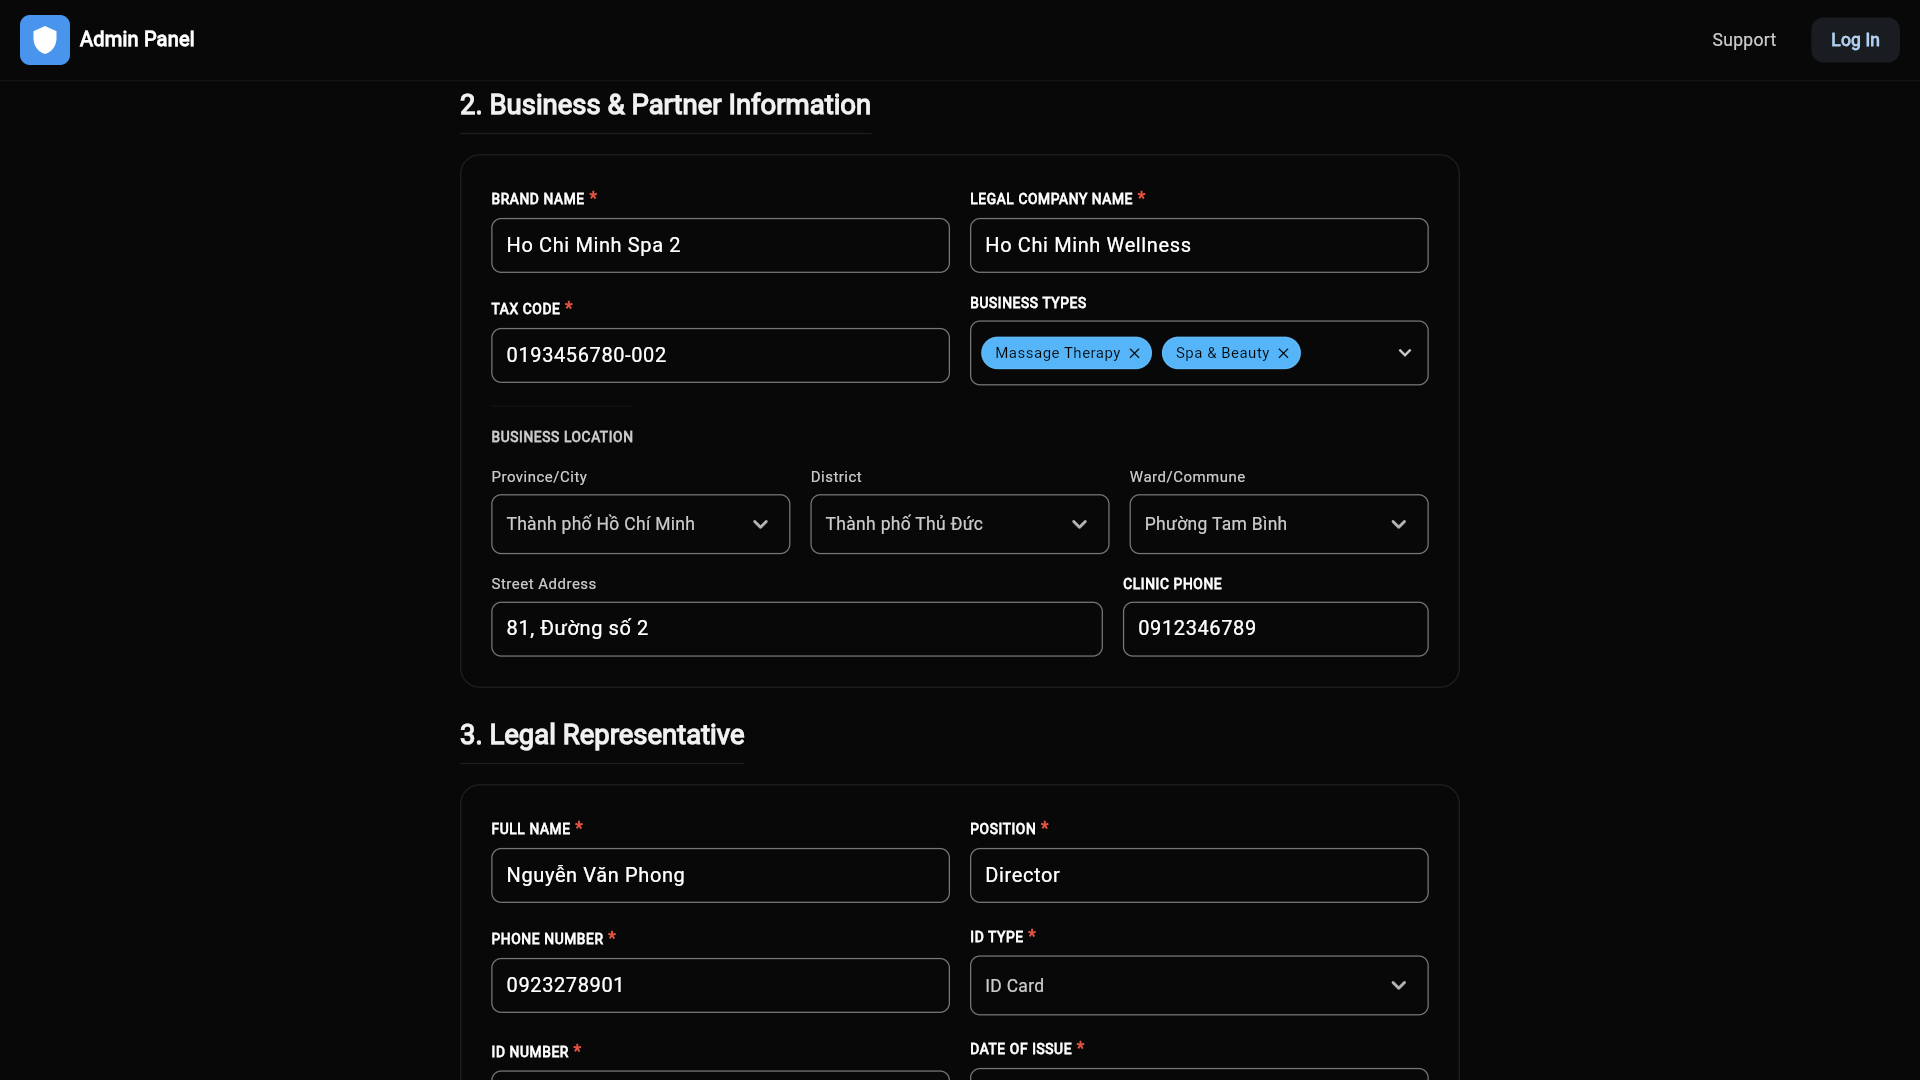
\includegraphics[width=\linewidth]{Images/Hiện thực/partner/fig_partner_reg_filled_business.png}
    \caption{Thông tin doanh nghiệp}
    \label{fig:partner_reg_business}
\end{subfigure}
\hfill
\begin{subfigure}[b]{0.48\linewidth}
    \centering
    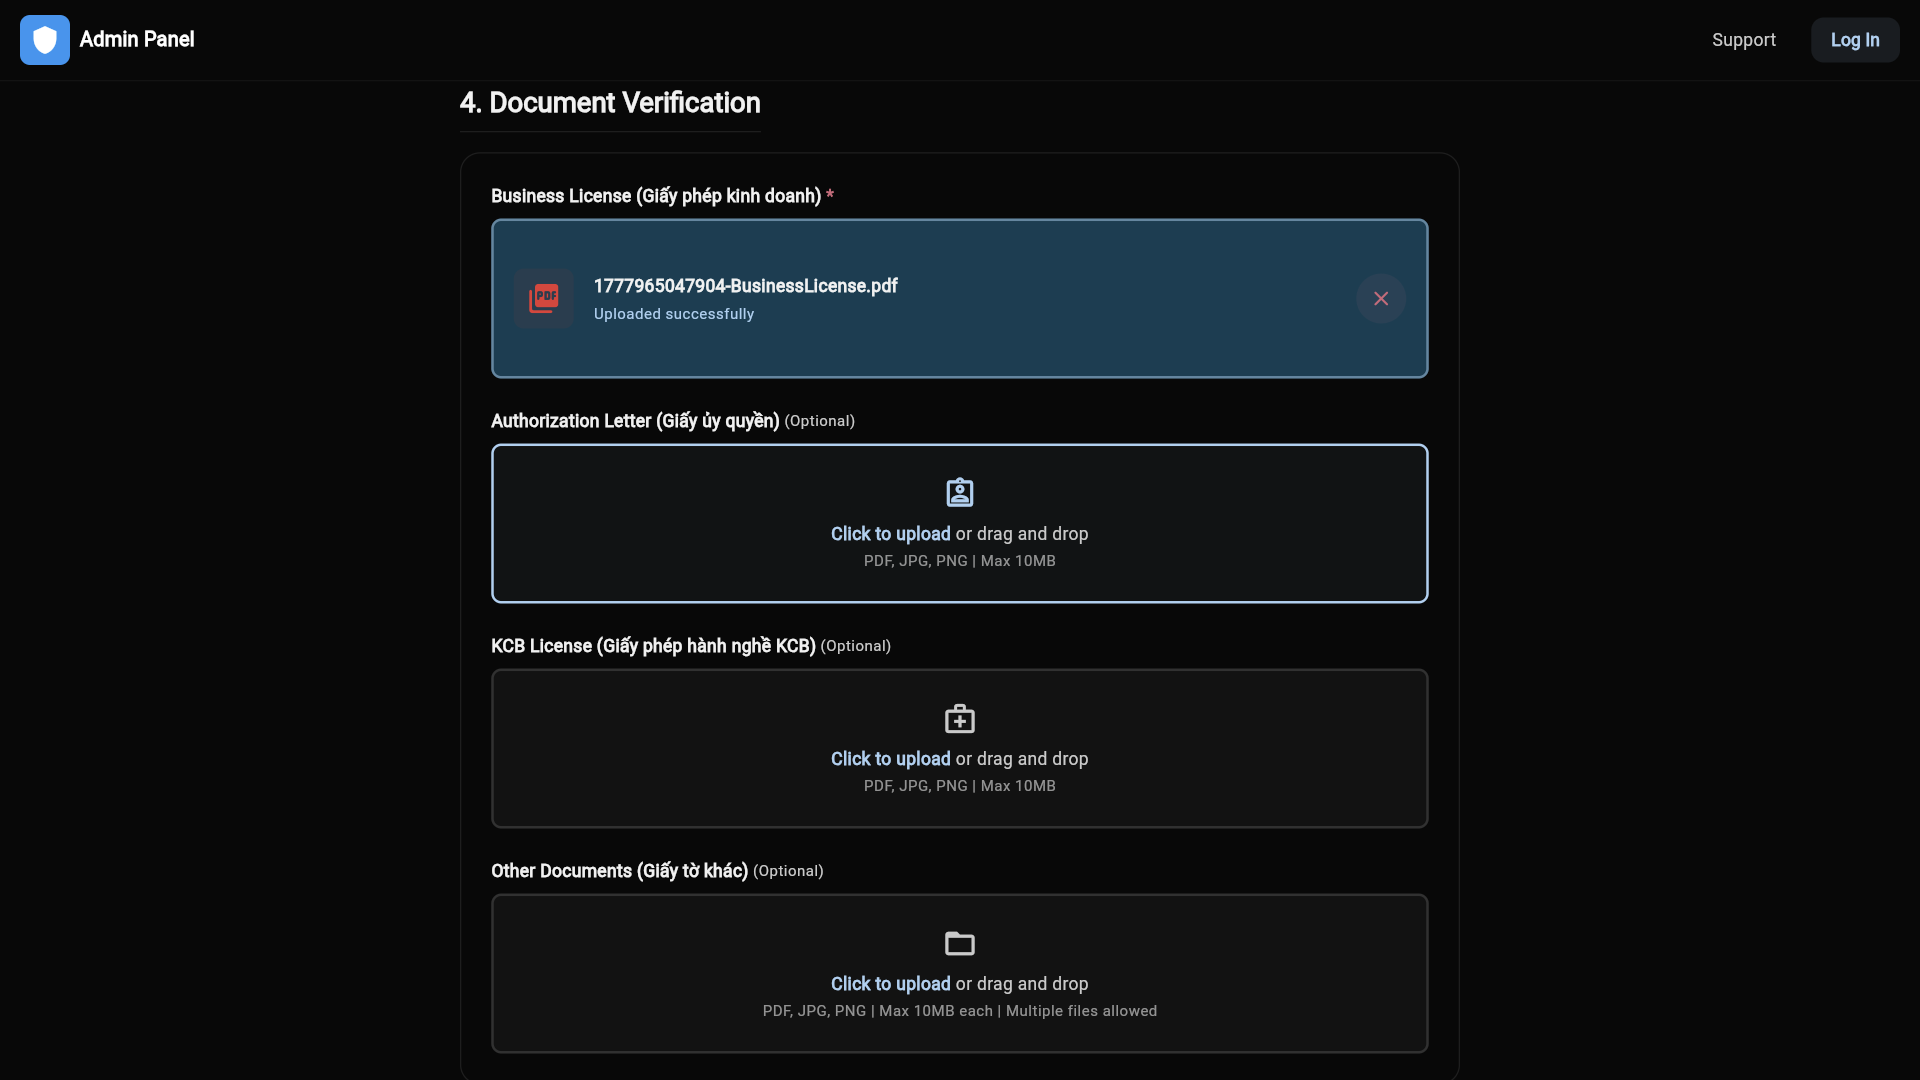
\includegraphics[width=\linewidth]{Images/Hiện thực/partner/fig_partner_reg_doc_uploaded.png}
    \caption{Tải giấy tờ KYC}
    \label{fig:partner_reg_docs}
\end{subfigure}
\par\medskip
\caption{Luồng đăng ký đối tác -- giai đoạn doanh nghiệp và hồ sơ}
\end{figure}

\begin{itemize}
    \item \textbf{Thao tác khai báo doanh nghiệp:} Đối tác điền tên pháp nhân, mã số thuế, địa chỉ và loại hình kinh doanh.
    \item \textbf{Thao tác nộp hồ sơ:} Đối tác tải lên bộ KYC và kiểm tra trạng thái upload trước khi gửi xét duyệt.
\end{itemize}

\begin{figure}[H]
    \centering
    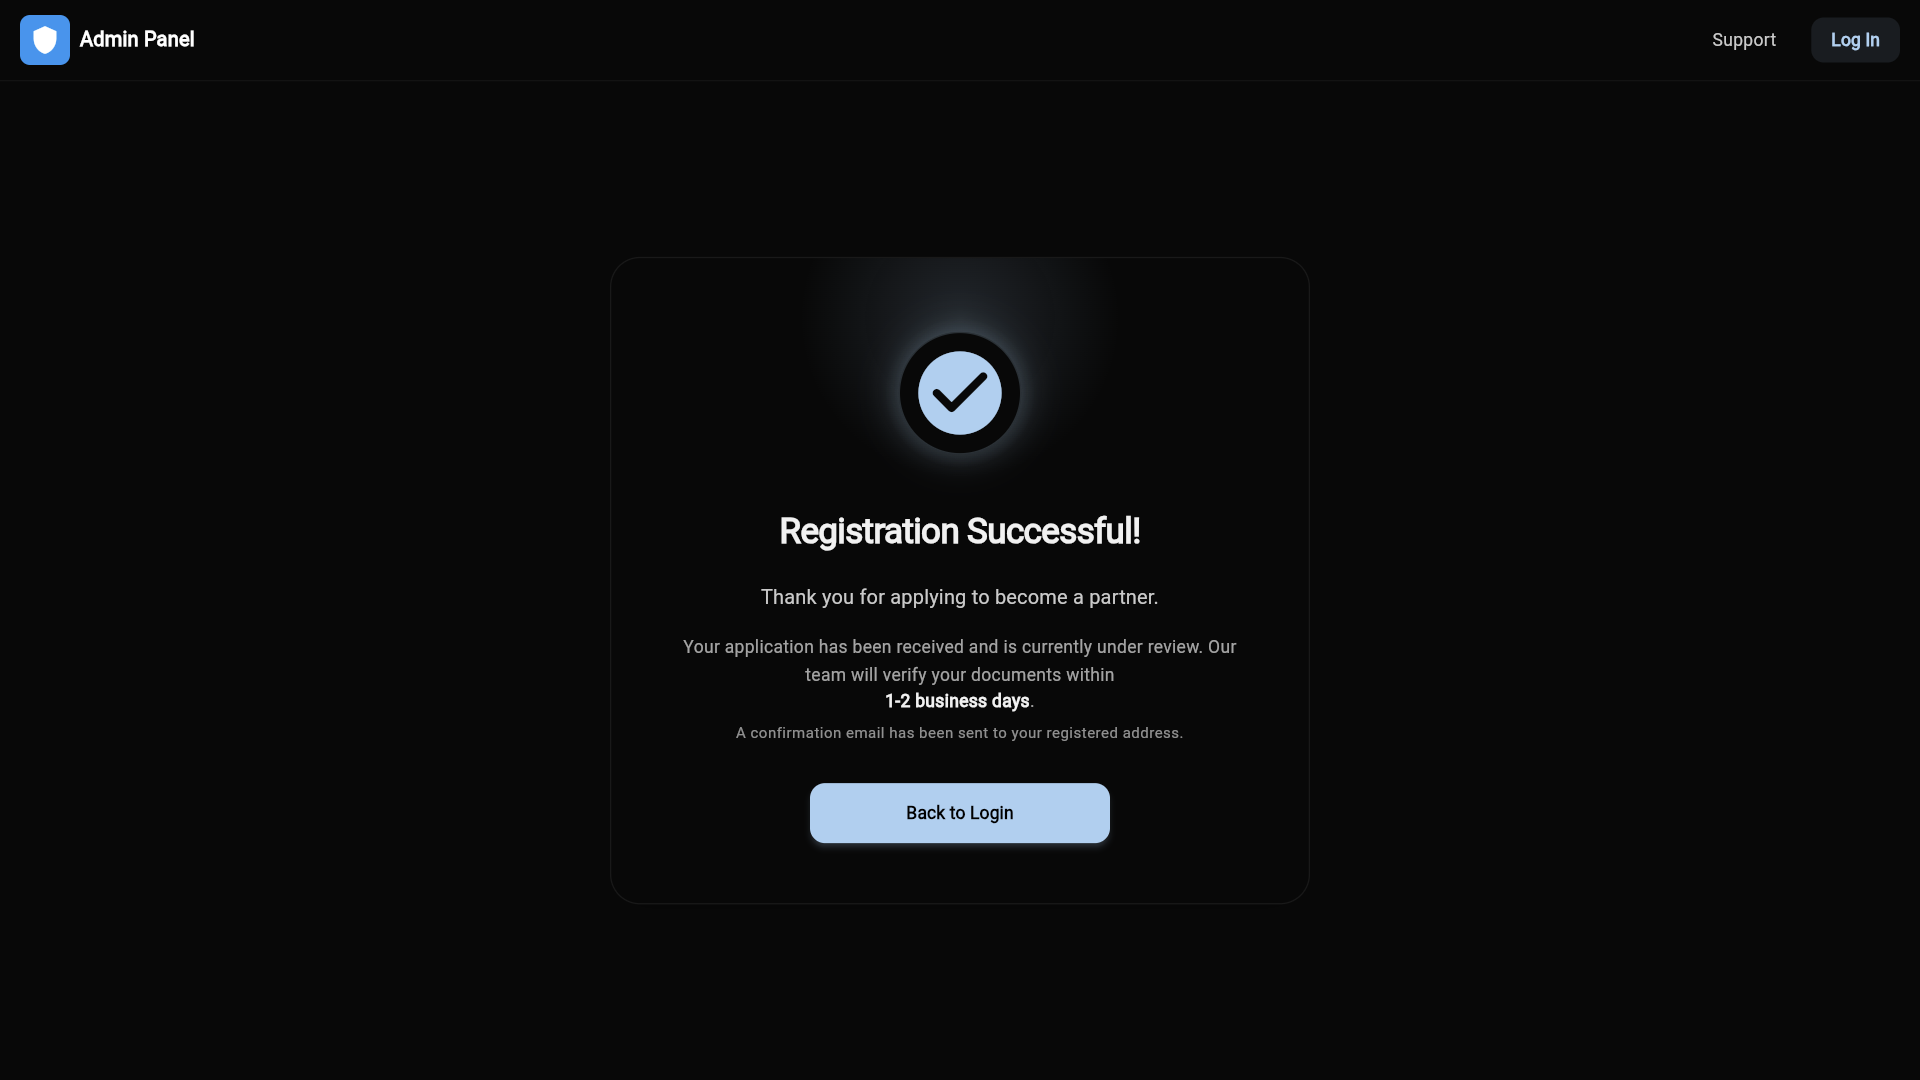
\includegraphics[width=0.85\textwidth]{Images/Hiện thực/partner/fig_partner_reg_success.png}
    \vspace{0.5em}
    \caption{Đăng ký đối tác thành công và chờ xét duyệt}
    \label{fig:partner_reg_success}
\end{figure}

\begin{itemize}
    \item \textbf{Kết quả thao tác:} Hệ thống xác nhận hồ sơ đã gửi thành công và chuyển trạng thái sang \texttt{PENDING}.
    \item \textbf{Bước tiếp theo:} Đối tác theo dõi phản hồi kiểm duyệt hoặc bổ sung hồ sơ khi có yêu cầu chỉnh sửa.
\end{itemize}

Khi đối tác chỉnh sửa hồ sơ (đặc biệt sau khi bị yêu cầu bổ sung), hệ thống áp dụng cơ chế cập nhật thông minh (Smart Update): nhận diện thay đổi qua \texttt{fieldKey}, phân loại mức độ nhạy cảm (mã số thuế, địa chỉ vs. số điện thoại), và tự động chuyển trạng thái phù hợp --- từ \texttt{REQUIRED\_RESUBMIT} về \texttt{PENDING} khi sửa xong lỗi, hoặc thu hồi \texttt{APPROVED} khi sửa thông tin nhạy cảm.

\subsubsection{Hoàn thiện Hồ sơ Công khai (Post-Verification)}

Sau khi được Admin phê duyệt (\texttt{APPROVED}), đối tác đăng nhập vào Partner Portal và được chuyển đến trang ``Complete Clinic Profile'' để hoàn thiện thông tin công khai --- phần dữ liệu sẽ hiển thị cho người dùng cuối trên ứng dụng di động. Quy trình hoàn thiện gồm các bước sau (Hình~\ref{fig:partner_clinic_empty} đến Hình~\ref{fig:partner_clinic_branding}):

\begin{enumerate}
    \item \textbf{Giới thiệu phòng khám (About Clinic):} Nhập mô tả tổng quan về cơ sở, chuyên môn, kinh nghiệm và phương pháp chăm sóc. Hệ thống yêu cầu tối thiểu 120 ký tự và kiểm tra tính sẵn sàng xuất bản.

    \item \textbf{Thư viện ảnh (Clinic Gallery):} Tải lên 3--8 hình ảnh minh họa không gian phòng khám, trang thiết bị, phòng trị liệu, và môi trường phục vụ bệnh nhân. Hỗ trợ sắp xếp thứ tự hiển thị bằng nút mũi tên.

    \item \textbf{Chứng chỉ tin cậy (Trust Badges):} Thêm các chứng nhận, tiêu chuẩn, hoặc giấy phép chuyên môn để tăng độ tin cậy.
\end{enumerate}

Thanh tiến trình ở cuối trang (``Required completion: X/4'') theo dõi số mục bắt buộc đã hoàn thành. Khi đạt 4/4, đối tác có thể nhấn ``Complete profile'' để công khai trang phòng khám.

\begin{figure}[H]
    \centering
    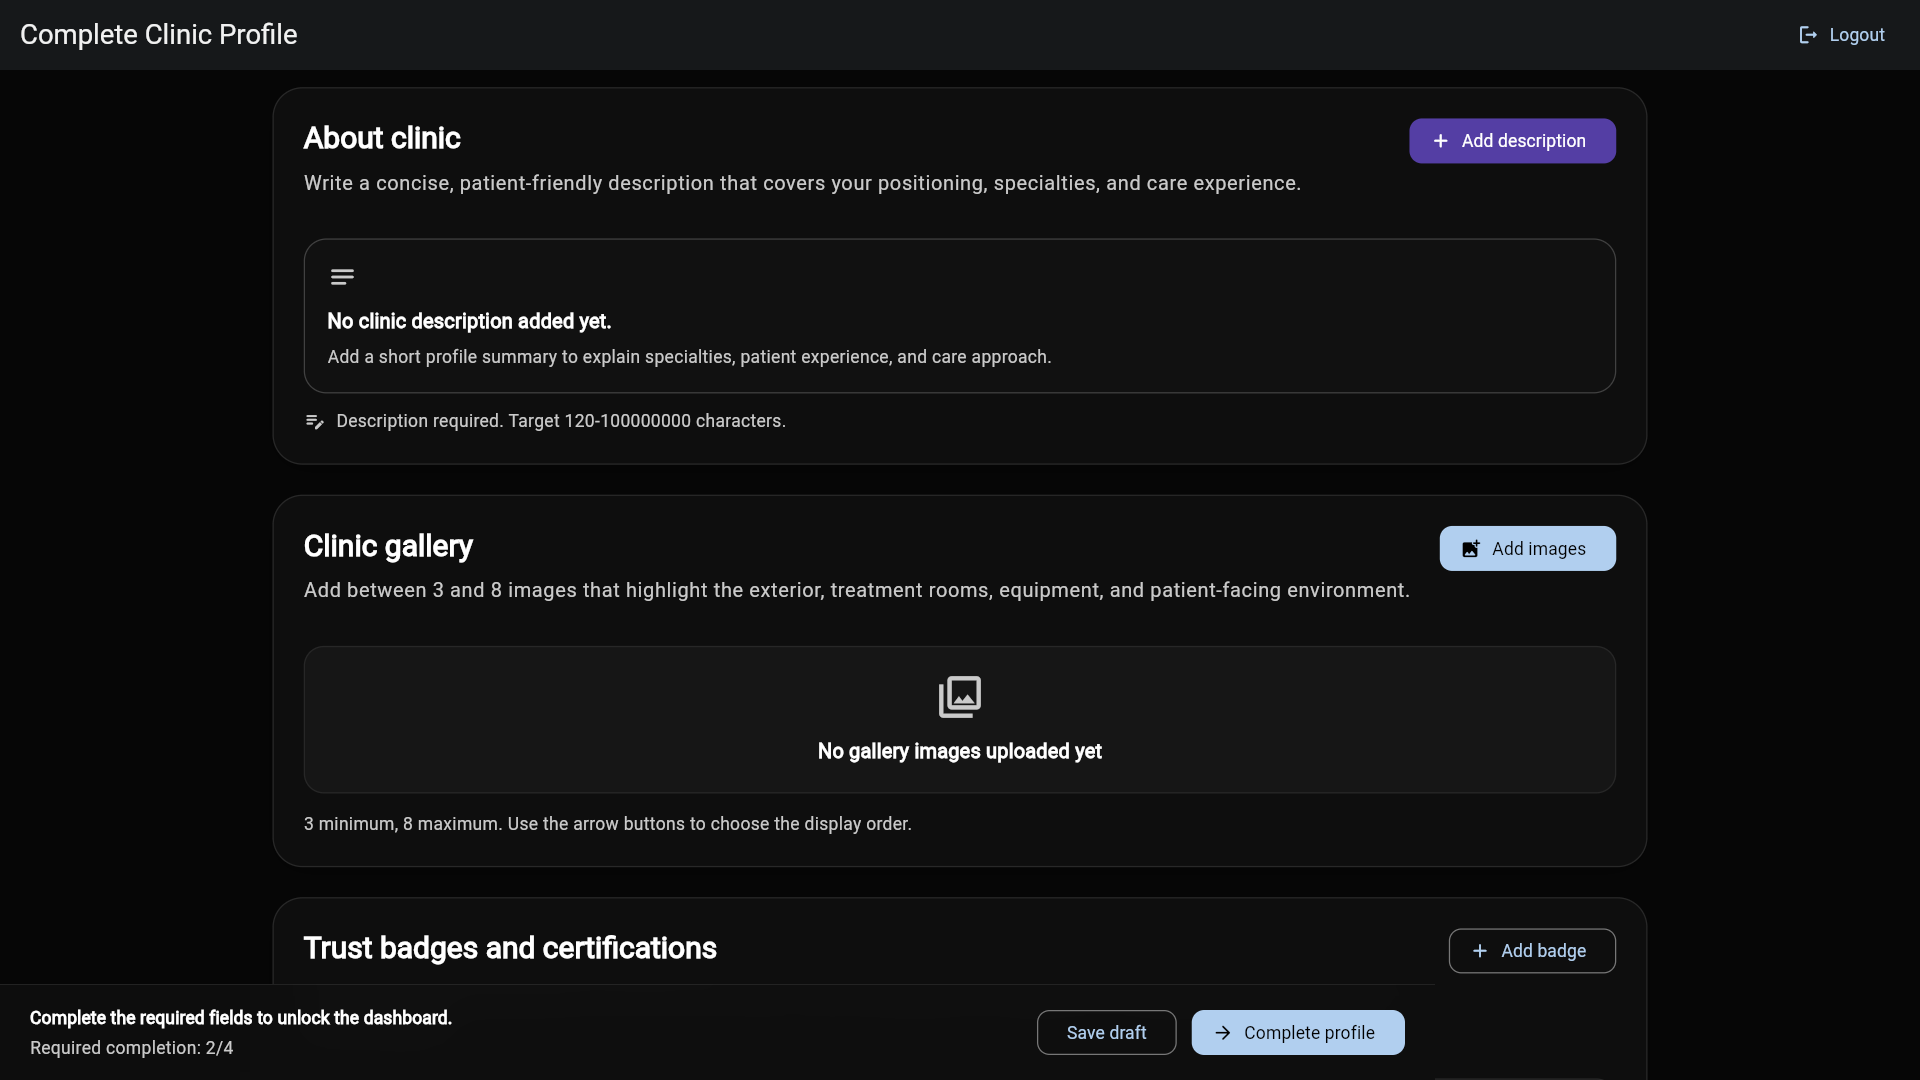
\includegraphics[width=0.92\textwidth]{Images/Hiện thực/partner/fig_partner_clinic_about_empty.png}
    \vspace{1em}
    \caption{Trang hoàn thiện hồ sơ phòng khám -- trạng thái chưa điền}
    \label{fig:partner_clinic_empty}
\end{figure}

\begin{itemize}
    \item \textbf{Trạng thái ban đầu:} Hai mục bắt buộc \textbf{About Clinic} và \textbf{Clinic Gallery} chưa được điền thông tin.
    \item \textbf{Thanh tiến trình (Progress Bar):} Hiển thị ``Required completion: 0/4'', giúp đối tác theo dõi tiến độ hoàn thiện hồ sơ.
\end{itemize}

\begin{figure}[H]
    \centering
    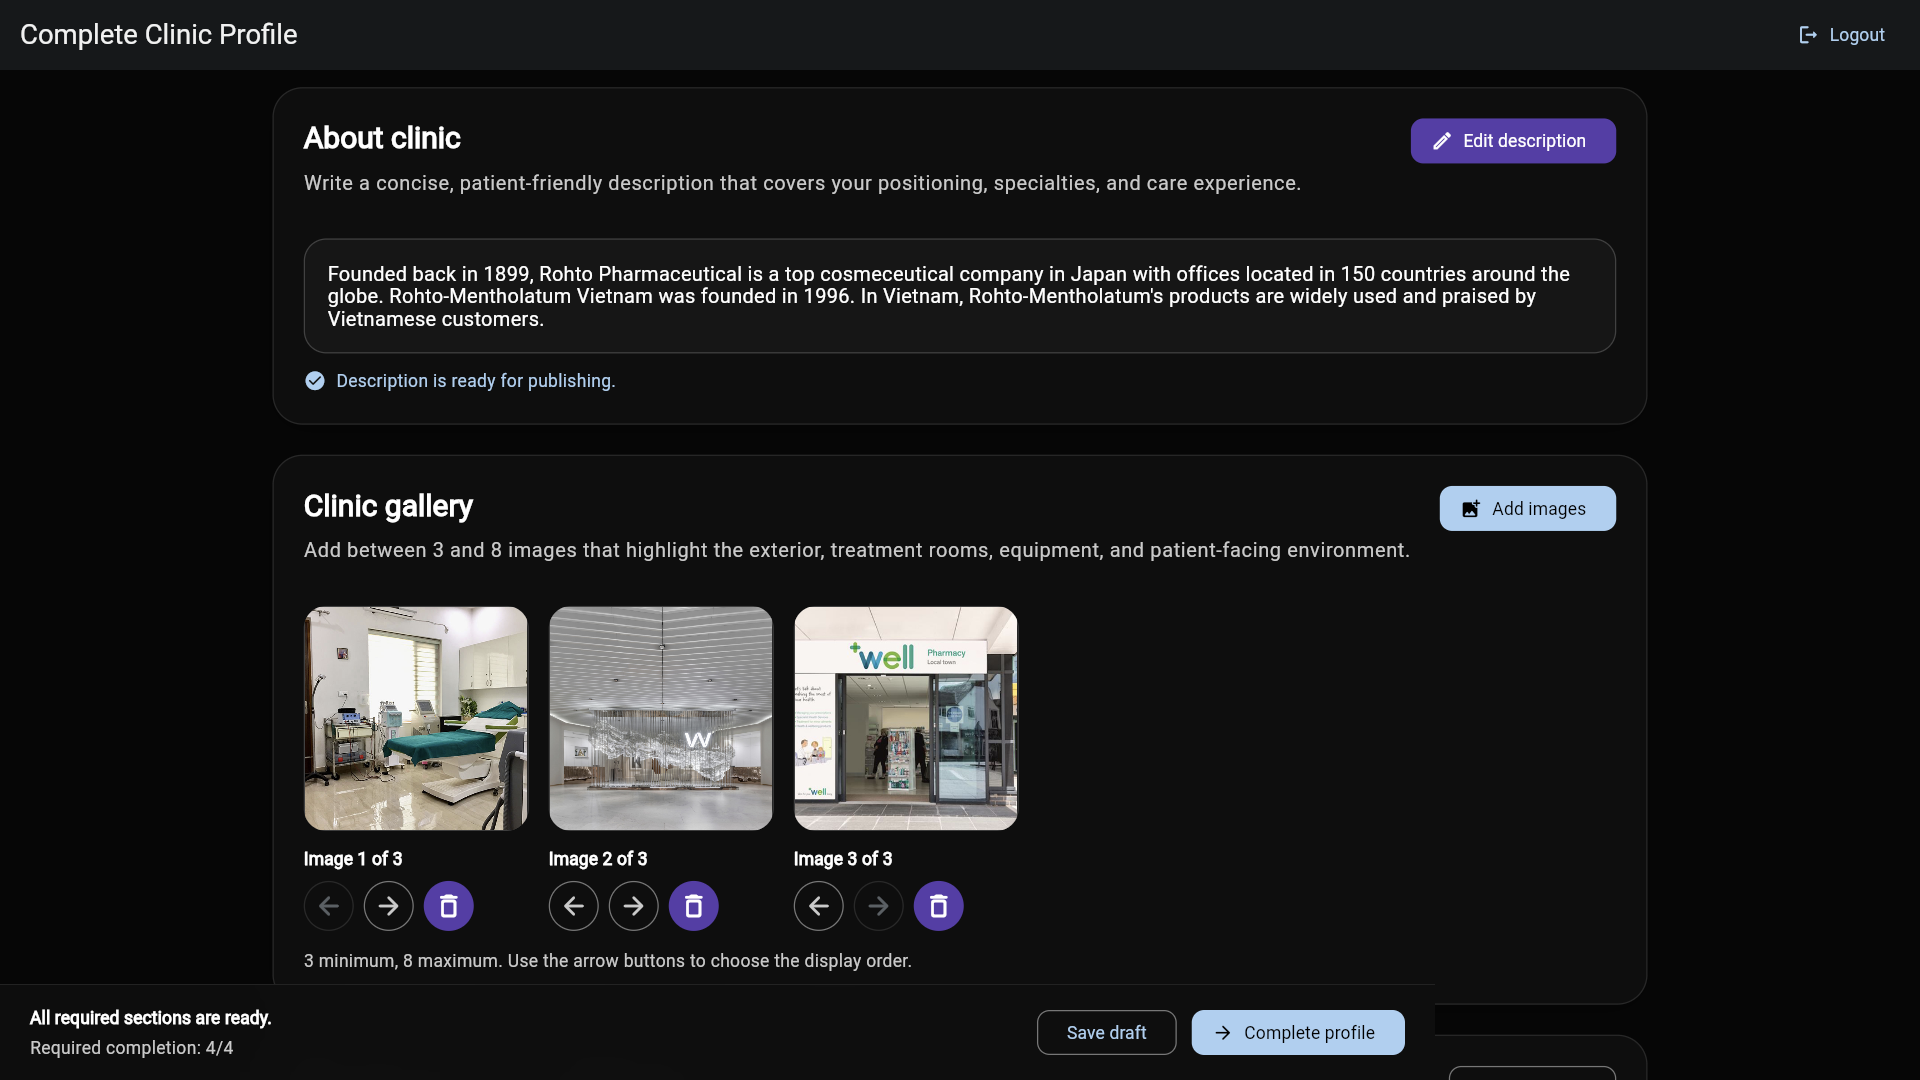
\includegraphics[width=0.92\textwidth]{Images/Hiện thực/partner/fig_partner_clinic_about_filled.png}
    \vspace{1em}
    \caption{Trang hoàn thiện hồ sơ -- đã điền About Clinic và Gallery}
    \label{fig:partner_clinic_filled}
\end{figure}

\begin{itemize}
    \item \textbf{About Clinic:} Nhập mô tả tổng quan về cơ sở (yêu cầu tối thiểu 120 ký tự).
    \item \textbf{Clinic Gallery:} Tải lên hình ảnh minh họa không gian phòng khám, hỗ trợ thao tác sắp xếp thứ tự hiển thị thông qua nút mũi tên lên/xuống.
\end{itemize}

\begin{figure}[H]
    \centering
    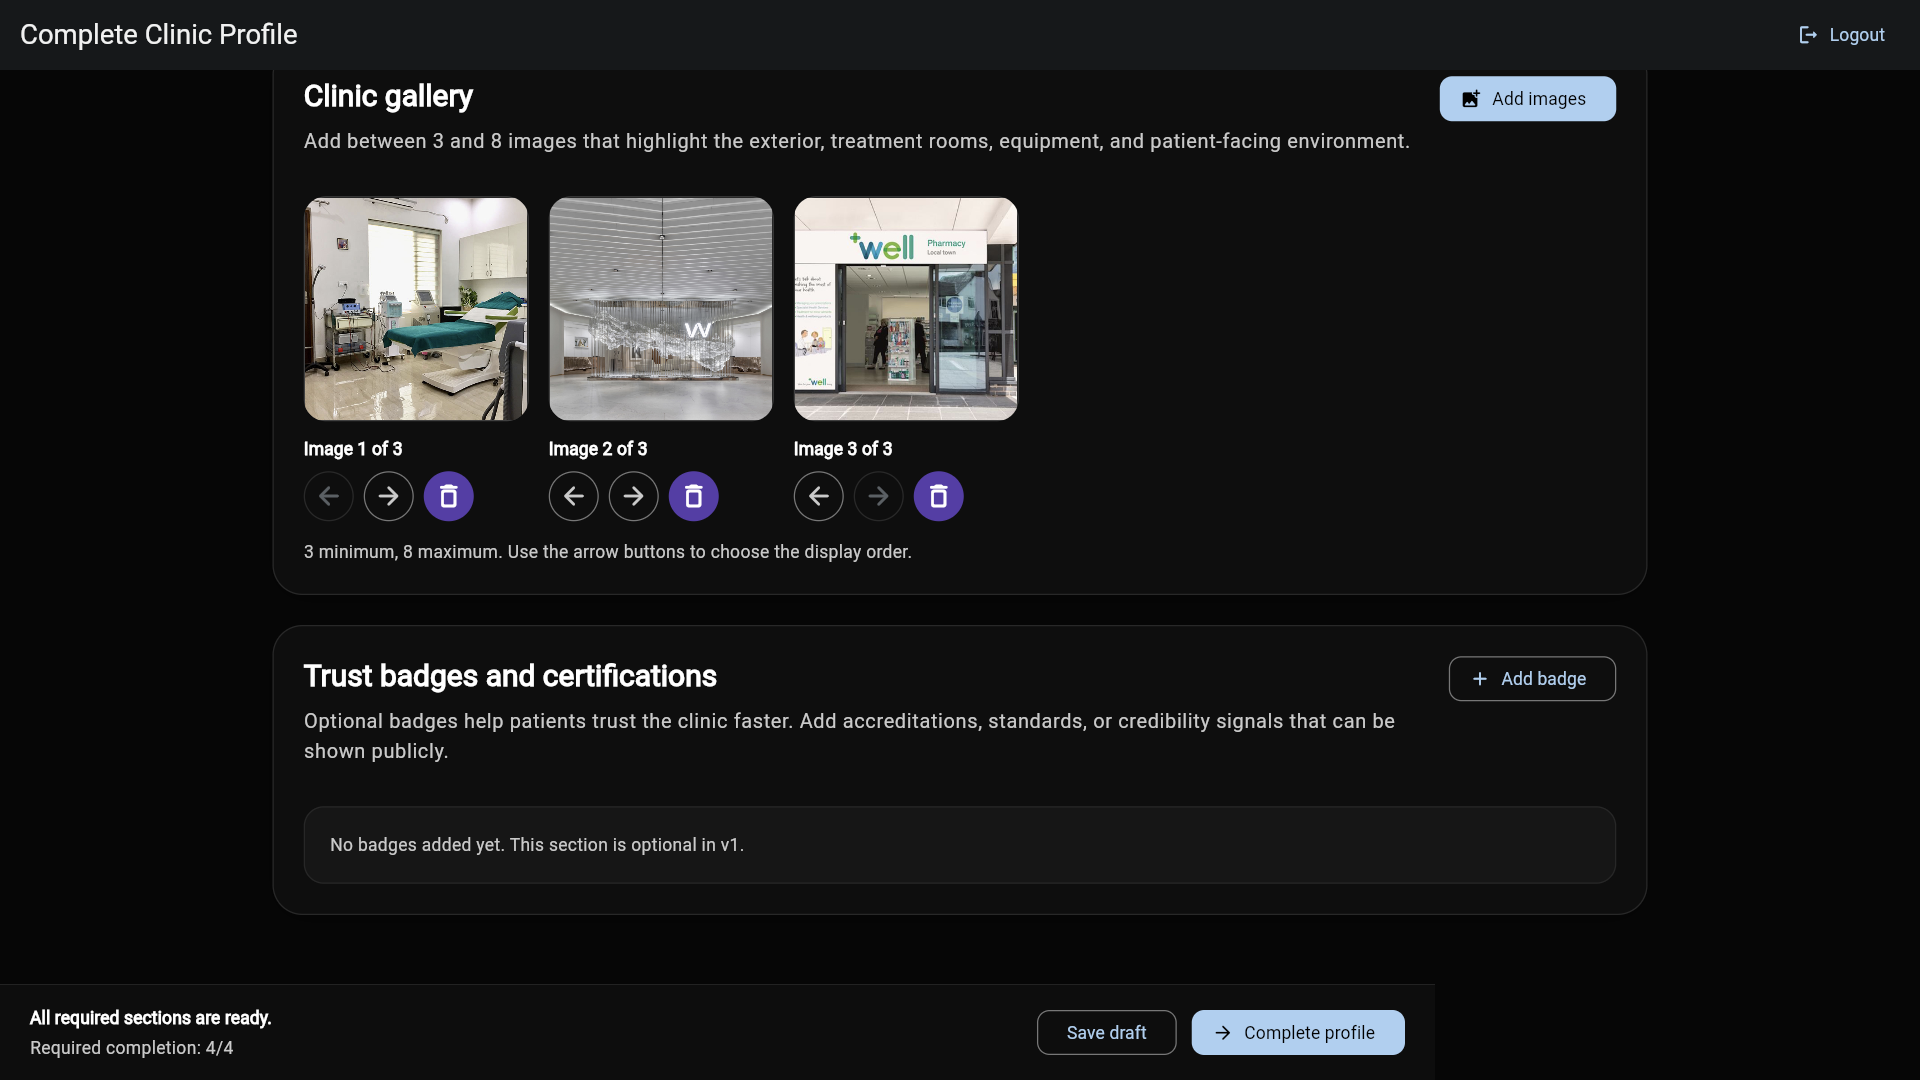
\includegraphics[width=0.92\textwidth]{Images/Hiện thực/partner/fig_partner_clinic_gallery_badges.png}
    \vspace{1em}
    \caption{Phần Trust Badges -- chứng chỉ tin cậy}
    \label{fig:partner_clinic_badges}
\end{figure}

\begin{itemize}
    \item \textbf{Chức năng:} Cho phép đối tác thêm các chứng nhận hoặc giấy phép chuyên môn để tăng độ uy tín.
    \item \textbf{Thông tin mỗi badge:} Bao gồm Title (Tiêu đề), Subtitle (Mô tả phụ), Icon (Biểu tượng), và thứ tự sắp xếp hiển thị.
\end{itemize}

\begin{figure}[H]
    \centering
    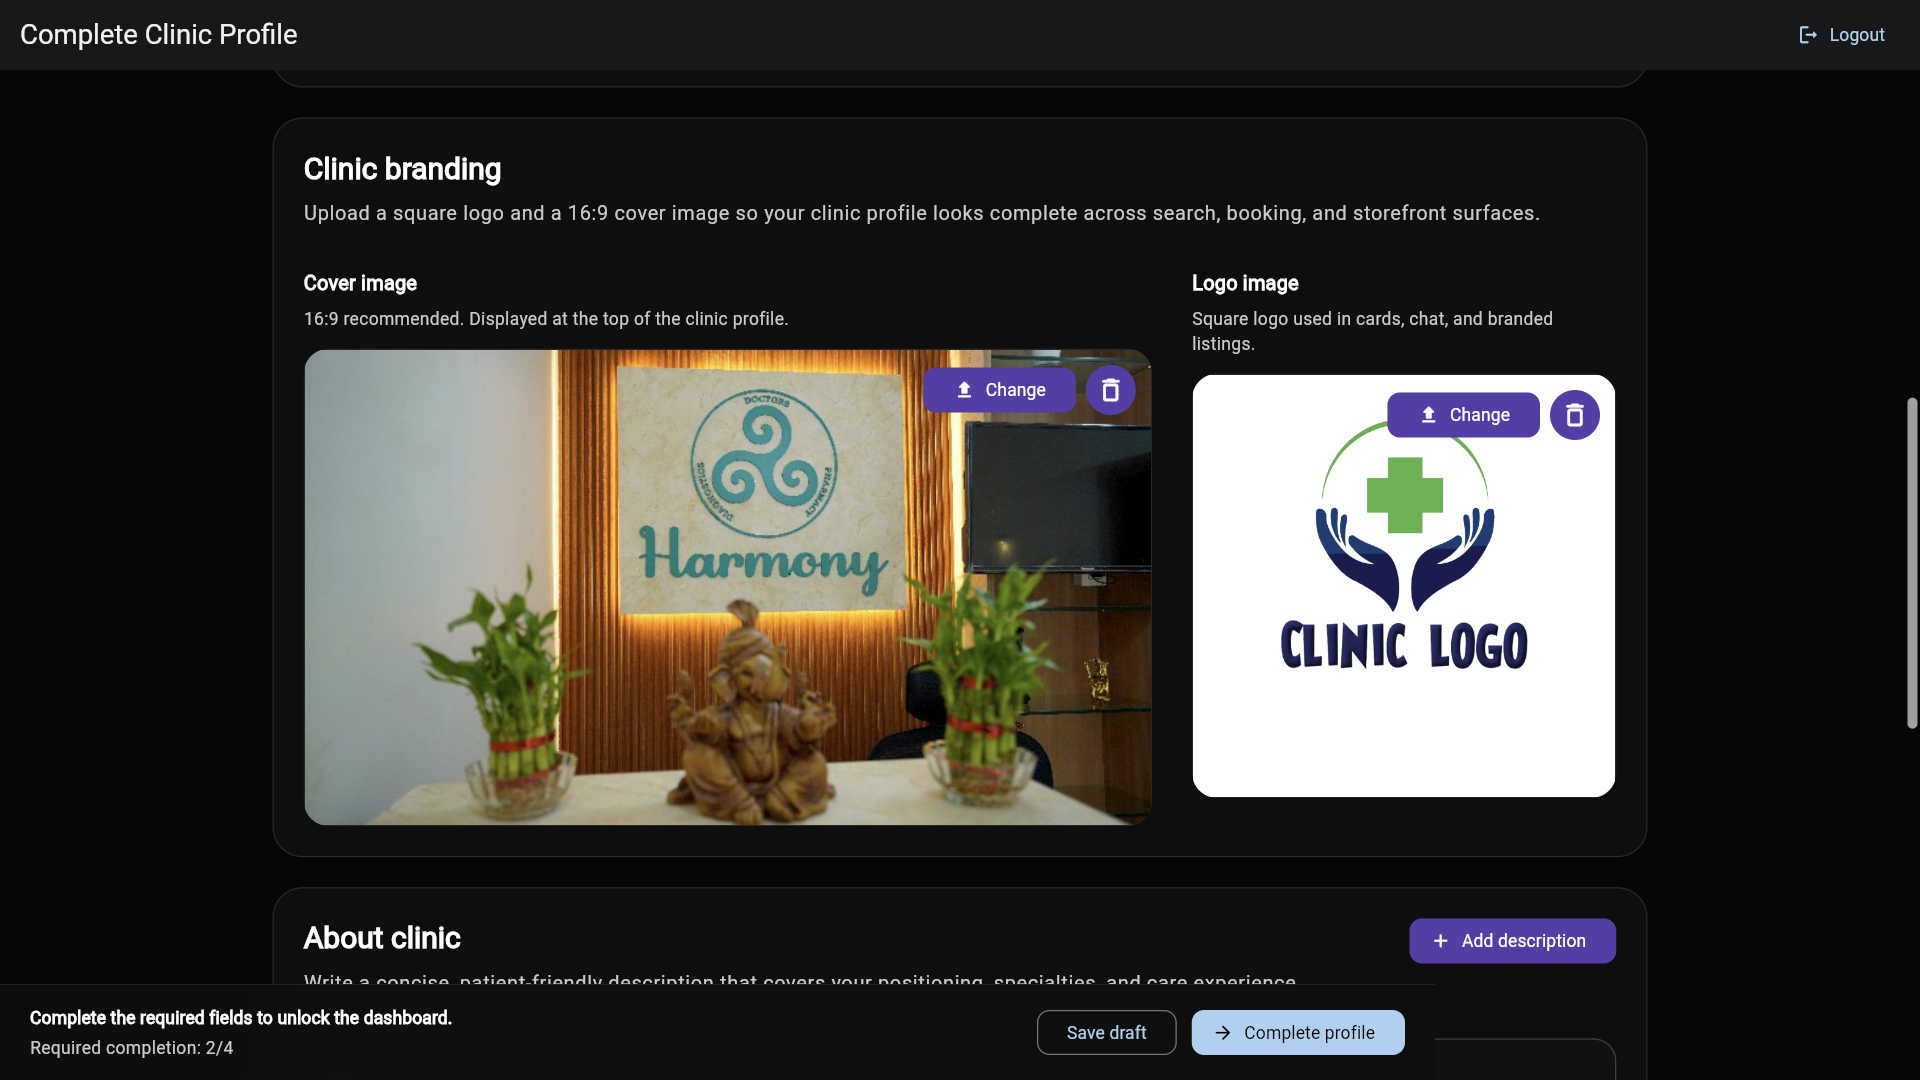
\includegraphics[width=0.92\textwidth]{Images/Hiện thực/partner/fig_partner_clinic_branding_complete.png}
    \vspace{1em}
    \caption{Phần Clinic Branding đã hoàn thiện}
    \label{fig:partner_clinic_branding}
\end{figure}

\begin{itemize}
    \item \textbf{Hình ảnh thương hiệu:} Đối tác đã tải lên ảnh bìa (Cover Image) và logo của phòng khám.
    \item \textbf{Vị trí hiển thị:} Hai hình ảnh này sẽ đóng vai trò nhận diện chính và hiển thị ở vị trí đầu tiên trên trang phòng khám trong ứng dụng di động của người dùng.
\end{itemize}

Dữ liệu từ quy trình này được tổng hợp và hiển thị trên trang chi tiết phòng khám phía người dùng (\texttt{GET /clinics/:id/info}).

\subsubsection{Quản lý Dịch vụ phía Đối tác}

\texttt{PartnerHealthServiceController} (prefix: \texttt{@PartnerApi('health-services')}) cho phép đối tác quản lý dịch vụ của mình:

\begin{itemize}
    \item \textbf{CRUD dịch vụ:} Tạo mới, cập nhật, xóa mềm dịch vụ (Product). Mỗi dịch vụ bao gồm thông tin cơ bản (tên, mô tả, giá gốc, giá khuyến mãi), định nghĩa chi tiết (\texttt{ProductDefinition}: thời lượng phút), và cấu hình hiển thị (\texttt{is\_visible\_online}).
    \item \textbf{Đa phương tiện:} Upload hình ảnh/video qua \texttt{ProductMedia}, hình ảnh cơ sở vật chất qua \texttt{ProductFacilityImage}.
    \item \textbf{Phân công chuyên gia:} Gán nhân viên đủ điều kiện thực hiện dịch vụ qua \texttt{ProductEmployeeEligibility} (quan hệ n-n giữa Product và Employee).
    \item \textbf{Phạm vi truy cập:} Đối tác chỉ được thao tác trên dịch vụ thuộc tổ chức mình. Guard kiểm tra \texttt{partnerId} từ JWT token.
\end{itemize}

Khi dịch vụ được tạo/cập nhật/xóa, hệ thống tự động publish event qua Redis Pub/Sub (\texttt{service:created}, \texttt{service:updated}, \texttt{service:deleted}) để Recommender Service đồng bộ vector store trong thời gian thực.

\subsubsection{Quản lý Nhân sự và Cơ sở}

\paragraph{Module Nhân viên (\texttt{EmployeesModule})}

Quản lý nhân viên, bác sĩ và chuyên gia trên nền tảng:

\begin{itemize}
    \item \texttt{PartnerEmployeesController}: Đối tác CRUD nhân viên, cập nhật lịch làm việc, chuyên môn và trạng thái hoạt động.
    \item \texttt{UserEmployeesController}: Người dùng xem thông tin, tìm kiếm theo chuyên khoa, xem lịch trống.
    \item \textbf{Hồ sơ chuyên biệt:} Mở rộng từ \texttt{Employee} thành \texttt{DoctorProfile} (chuyên khoa, giấy phép hành nghề, \texttt{experience\_years}) và \texttt{TherapistProfile} (phương pháp trị liệu, kinh nghiệm).
\end{itemize}

\paragraph{Module Phòng khám (\texttt{ClinicModule} --- phía Đối tác)}

Quản lý phòng khám và cơ sở dịch vụ: tên, mô tả, hình ảnh, giờ hoạt động. Liên kết \texttt{Address} và tọa độ địa lý (PostGIS) phục vụ tìm kiếm theo vị trí.

\subsubsection{Tiếp nhận Lịch hẹn và Giao tiếp với Khách hàng}

Đối tác tiếp nhận và xử lý lịch hẹn từ khách hàng thông qua giao diện Partner Portal. Khi có booking mới, hệ thống tự động gửi thông báo qua \texttt{NotificationModule}. Đối tác có thể xác nhận hoặc từ chối lịch hẹn, với mọi thay đổi trạng thái được ghi nhận trong \texttt{BookingStatusLog}.

\paragraph{Chat phía Đối tác}

Đối xứng với phía người dùng, đối tác có hệ thống chat riêng:

\begin{itemize}
    \item \textbf{\texttt{PartnerChatController}:} REST API quản lý danh sách cuộc trò chuyện, lịch sử tin nhắn (phân trang), đánh dấu đã đọc, và hỗ trợ tệp đính kèm (\texttt{PartnerChatAttachment}).
    \item \textbf{\texttt{PartnerChatGateway}:} WebSocket Gateway xử lý nhắn tin thời gian thực phía đối tác. Tích hợp \texttt{ChatNotificationGateway} để đẩy thông báo tin nhắn mới khi đối tác không ở trong màn hình chat.
    \item \textbf{Xác thực:} Sử dụng chung middleware \texttt{ws-jwt-auth} với phía người dùng, phân biệt role qua JWT payload.
\end{itemize}

\subsubsection{Dashboard Đối tác (\texttt{DashboardPartnerModule})}

Cung cấp bảng điều khiển phân tích nghiệp vụ cho đối tác thông qua \texttt{PartnerDashboardController}, bao gồm các endpoint:

\begin{itemize}
    \item \textbf{\texttt{GET /stats}:} Thống kê KPI tổng hợp (doanh thu, số booking, tỷ lệ hoàn thành) theo kỳ tuần/tháng/quý.
    \item \textbf{\texttt{GET /revenue}:} Dữ liệu doanh thu time-series phục vụ vẽ biểu đồ xu hướng.
    \item \textbf{\texttt{GET /appointments/upcoming}:} Danh sách lịch hẹn sắp tới cần xử lý.
    \item \textbf{\texttt{GET /services/performance}:} Xếp hạng hiệu suất dịch vụ theo doanh thu và lượt đặt.
    \item \textbf{\texttt{GET /employees/distribution}:} Thống kê phân bố nhân sự theo vai trò.
    \item \textbf{\texttt{GET /reviews/recent}:} Đánh giá gần nhất từ khách hàng.
    \item \textbf{\texttt{GET /staff/schedule}:} Lịch nhân viên theo ngày cụ thể.
    \item \textbf{\texttt{GET /notifications}:} Thông báo và cảnh báo cho đối tác.
    \item \textbf{\texttt{GET /inventory/alerts}:} Cảnh báo về thiết bị hoặc vật tư cần bổ sung.
\end{itemize}

Toàn bộ endpoint bảo vệ bởi \texttt{@PartnerApi} decorator, đảm bảo đối tác chỉ xem dữ liệu thuộc tổ chức mình. Giao diện Dashboard (Hình~\ref{fig:partner_dashboard}) hiển thị tổng quan kinh doanh gồm: (1)~Doanh thu tổng, (2)~Số lịch hẹn, (3)~Dịch vụ đang hoạt động, (4)~Đánh giá trung bình, cùng biểu đồ doanh thu theo thời gian và các thao tác nhanh (Quick Actions) để thêm dịch vụ, nhân viên, hoặc quản lý tin nhắn.

\begin{figure}[H]
    \centering
    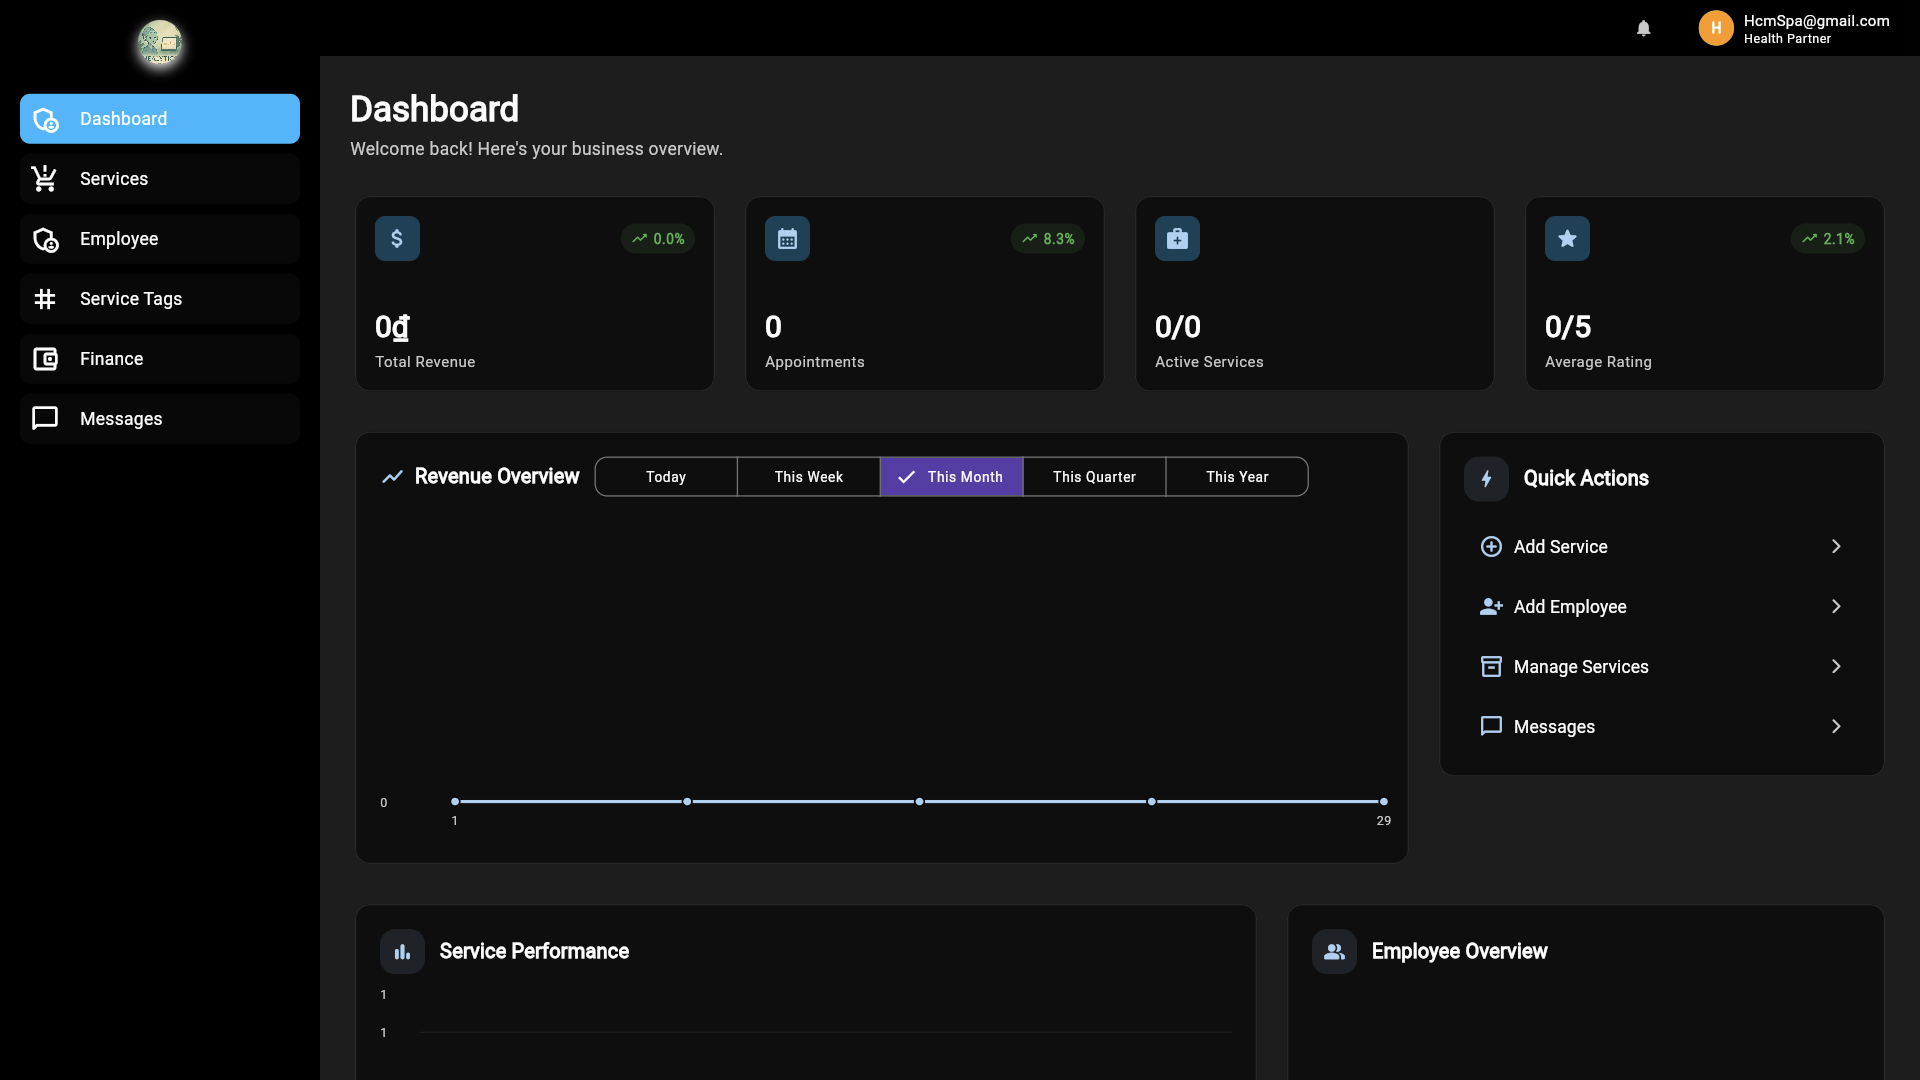
\includegraphics[width=0.85\textwidth]{Images/Hiện thực/partner/fig_partner_dashboard.png}
    \vspace{1em}
    \caption{Dashboard Đối tác -- tổng quan kinh doanh}
    \label{fig:partner_dashboard}
\end{figure}

\begin{itemize}
    \item \textbf{KPI tổng hợp:} Bao gồm (1)~Doanh thu tổng, (2)~Số lịch hẹn, (3)~Dịch vụ đang hoạt động, và (4)~Đánh giá trung bình.
    \item \textbf{Biểu đồ phân tích:} Cung cấp biểu đồ trực quan hóa xu hướng doanh thu theo thời gian.
    \item \textbf{Quick Actions (Thao tác nhanh):} Cho phép truy cập nhanh để thêm dịch vụ, quản lý nhân viên, hoặc kiểm tra tin nhắn khách hàng.
\end{itemize}


% ===========================================================================
% 6.3.4  PHÂN HỆ TRANG QUẢN TRỊ (ADMIN PORTAL)
% ===========================================================================
\subsection{Hiện thực Phân hệ Trang Quản trị (Admin Portal)}

Phân hệ Quản trị cung cấp cho quản trị viên công cụ giám sát và kiểm duyệt toàn bộ hệ thống. Admin đăng nhập qua trang đăng nhập chuyên biệt và truy cập vào hệ thống quản trị với 5 module chính: Dashboard, Finance, Category, Provider, và Notifications.

\begin{figure}[H]
    \centering
    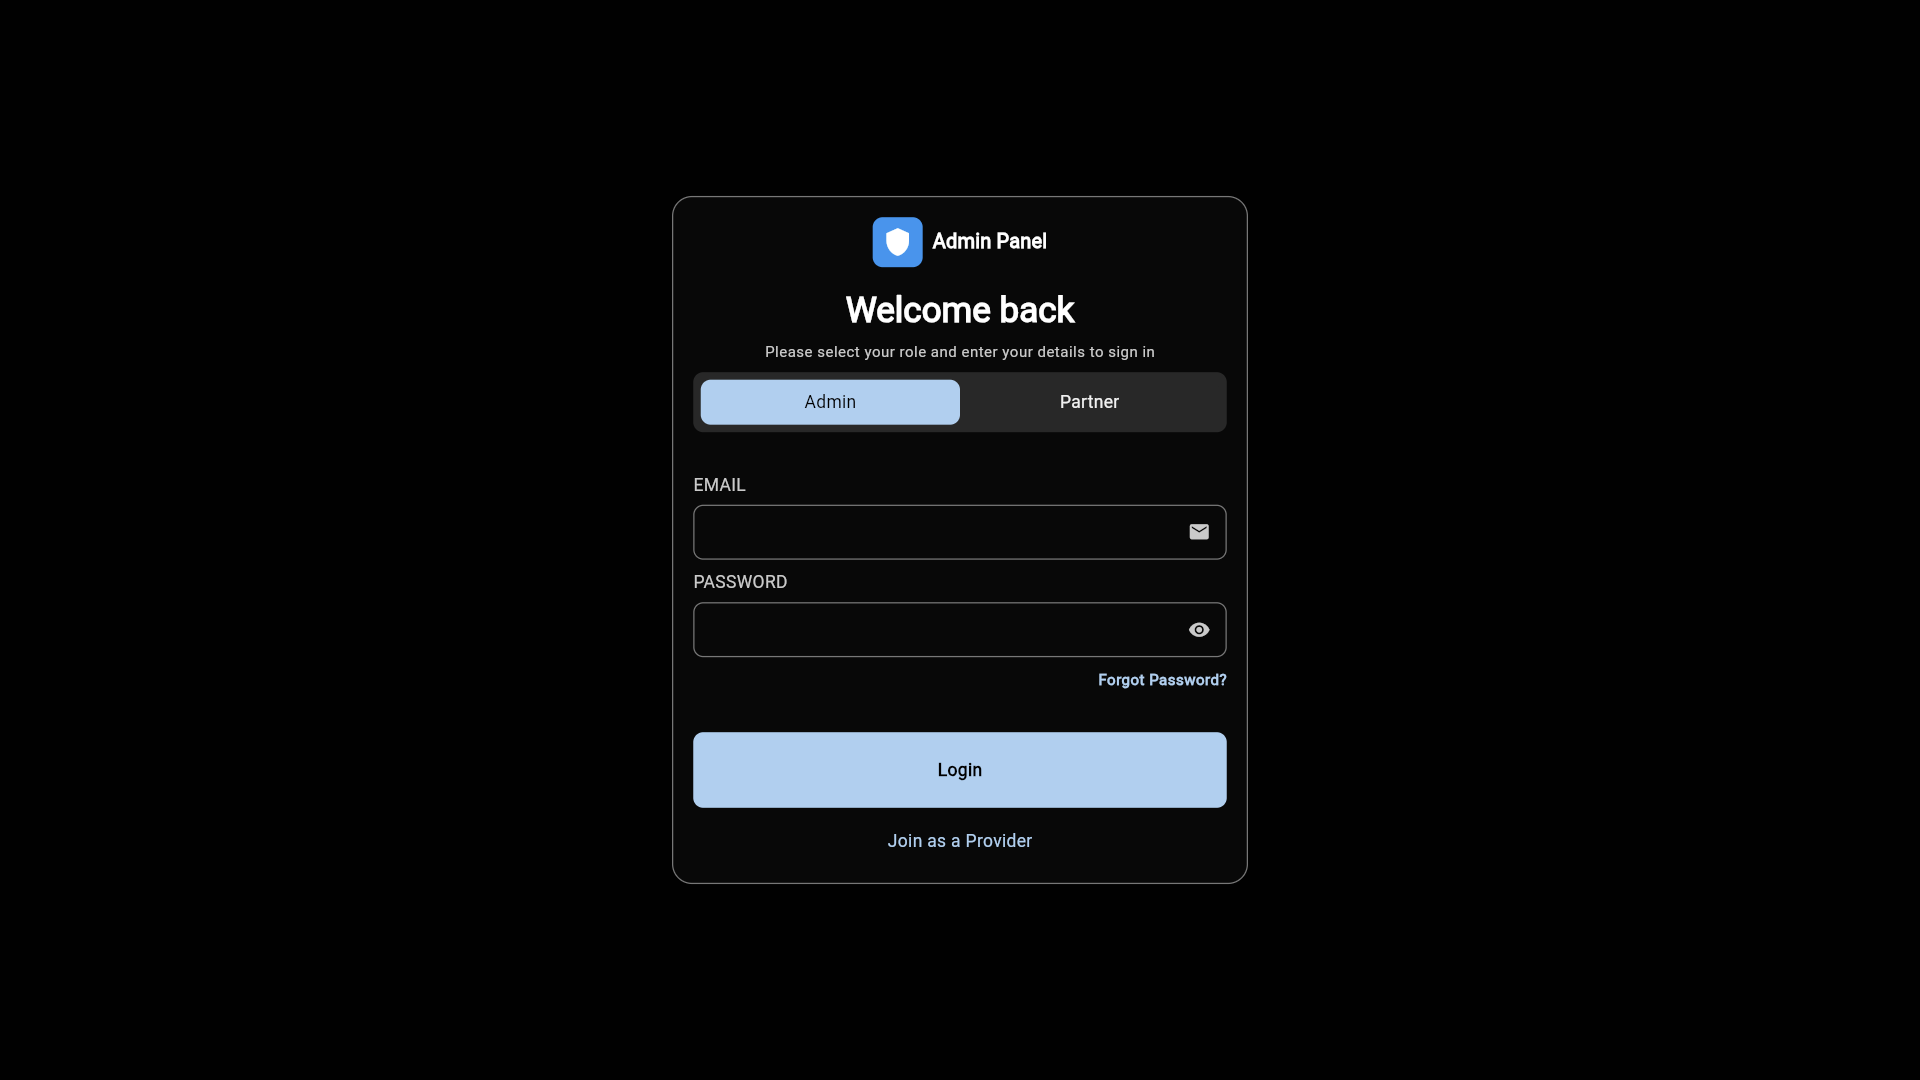
\includegraphics[width=0.6\textwidth]{Images/Hiện thực/admin/fig_admin_login.png}
    \vspace{1em}
    \caption{Màn hình đăng nhập Admin Portal}
    \label{fig:admin_login}
\end{figure}

\begin{itemize}
    \item \textbf{Thao tác xác thực:} Quản trị viên nhập tài khoản quản trị để truy cập hệ thống.
    \item \textbf{Thao tác điều hướng sau đăng nhập:} Hệ thống chuyển thẳng tới Dashboard tổng quan.
\end{itemize}

\begin{enumerate}
    \item \textbf{KPI Cards (hàng trên):} Doanh thu tổng (Gross Revenue), số giao dịch thành công, tổng số đối tác, tỷ lệ booking thành công, tỷ lệ thất bại, tỷ lệ hủy, giá trị booking trung bình, và số lượng thông báo vận hành.

    \item \textbf{Finance Trend (giữa):} Biểu đồ xu hướng doanh thu theo ngày (gross revenue, net revenue, refund pressure) kèm Finance Summary tổng hợp các chỉ số tài chính cốt lõi.

    \item \textbf{Booking Outcomes \& Transaction Health (dưới):} Phân tích chi tiết kết quả booking (Successful/Failed/Canceled) và sức khỏe giao dịch (Paid/Pending/Refunded/Failed/Canceled).

    \item \textbf{Top Revenue Partners \& Services:} Xếp hạng 5 đối tác và 5 dịch vụ có doanh thu cao nhất, kèm số booking và tỷ lệ thành công.
\end{enumerate}

\begin{figure}[H]
    \centering
    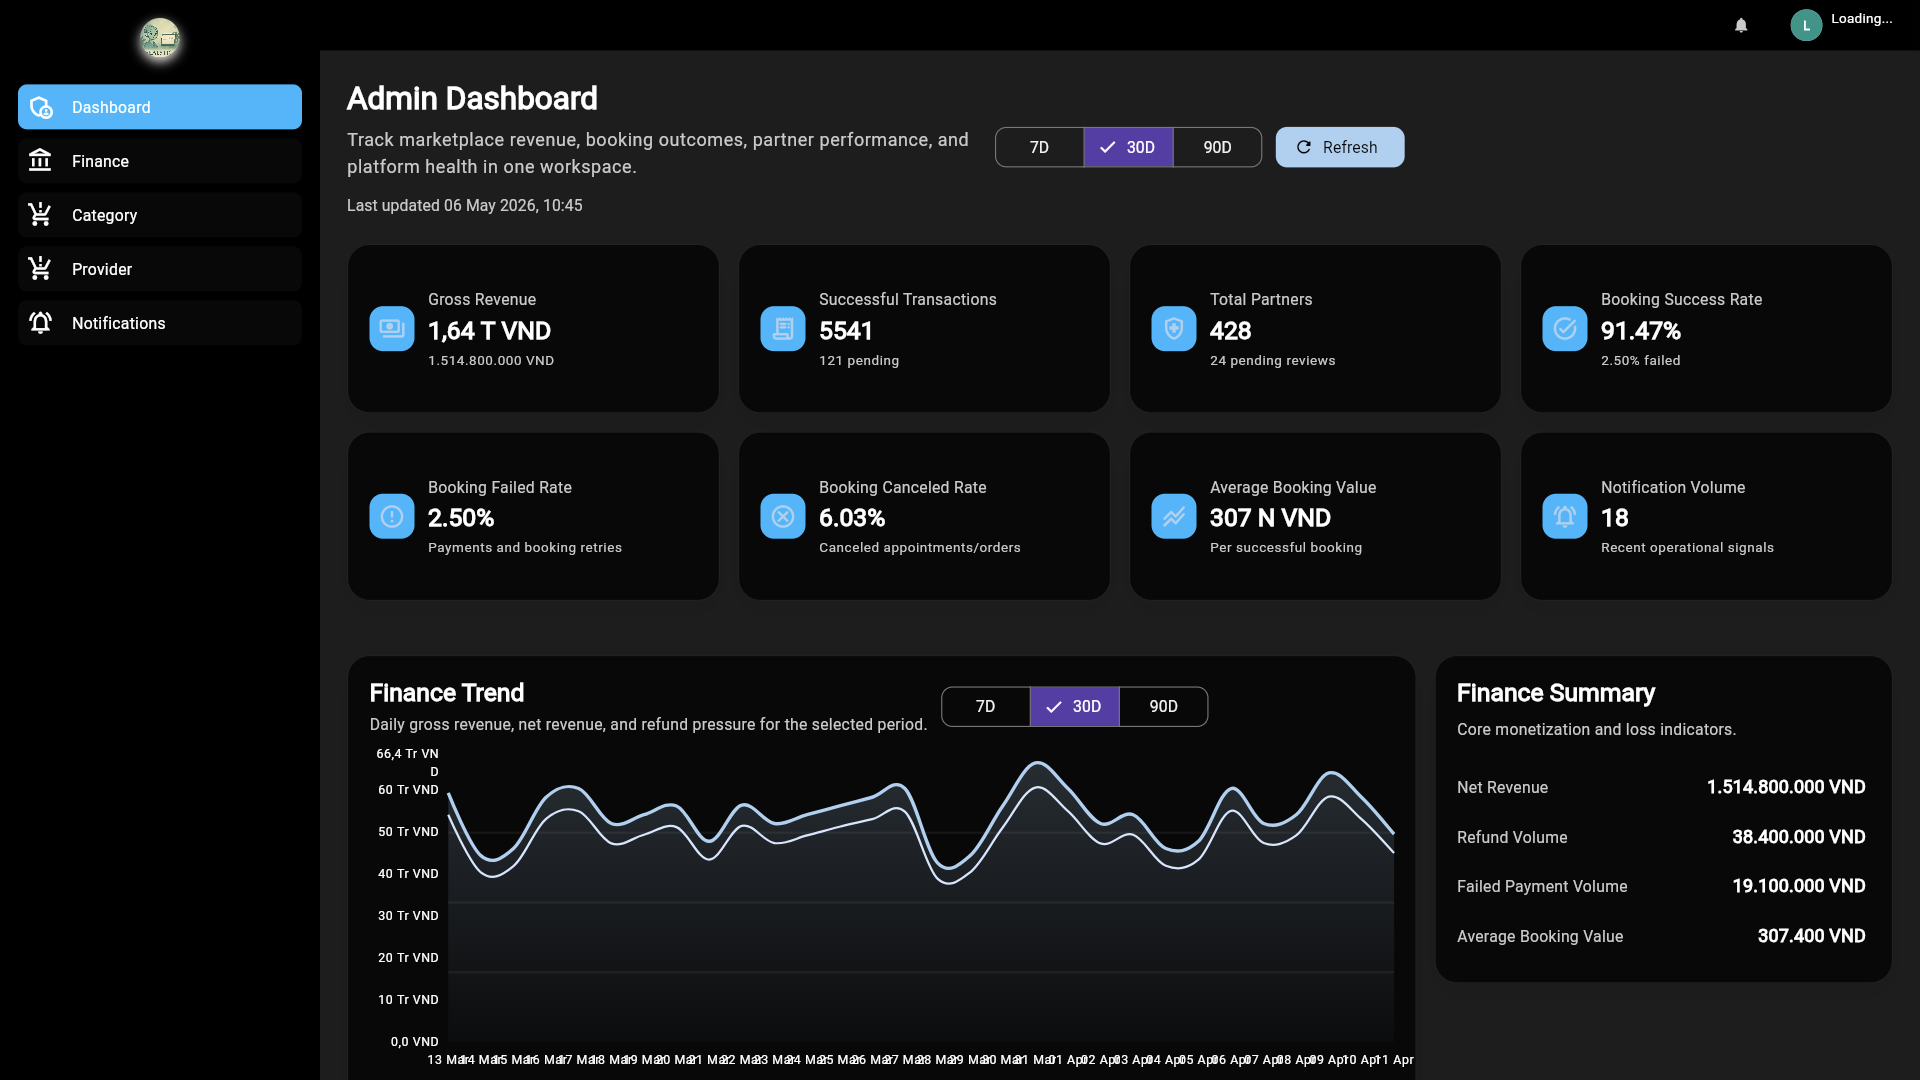
\includegraphics[width=0.92\textwidth]{Images/Hiện thực/admin/fig_admin_dashboard_top.png}
    \vspace{1em}
    \caption{Admin Dashboard -- phần trên: KPI Cards và Finance Trend}
    \label{fig:admin_dashboard_top}
\end{figure}

Hình~\ref{fig:admin_dashboard_top} hiển thị phần trên của Dashboard quản trị:
\begin{itemize}
    \item \textbf{Hàng KPI Cards:} Trình bày 8 chỉ số cốt lõi bao gồm Gross Revenue (Doanh thu tổng), Successful Transactions (Giao dịch thành công), Total Partners (Tổng đối tác, kèm số lượng chờ duyệt), tỷ lệ Booking (Thành công/Thất bại/Hủy), Average Booking Value (Giá trị trung bình), và Notification Volume.
    \item \textbf{Finance Trend:} Biểu đồ minh họa doanh thu trong 30 ngày qua, đi kèm với bảng tóm tắt tài chính (Finance Summary) chi tiết.
\end{itemize}

\begin{figure}[H]
    \centering
    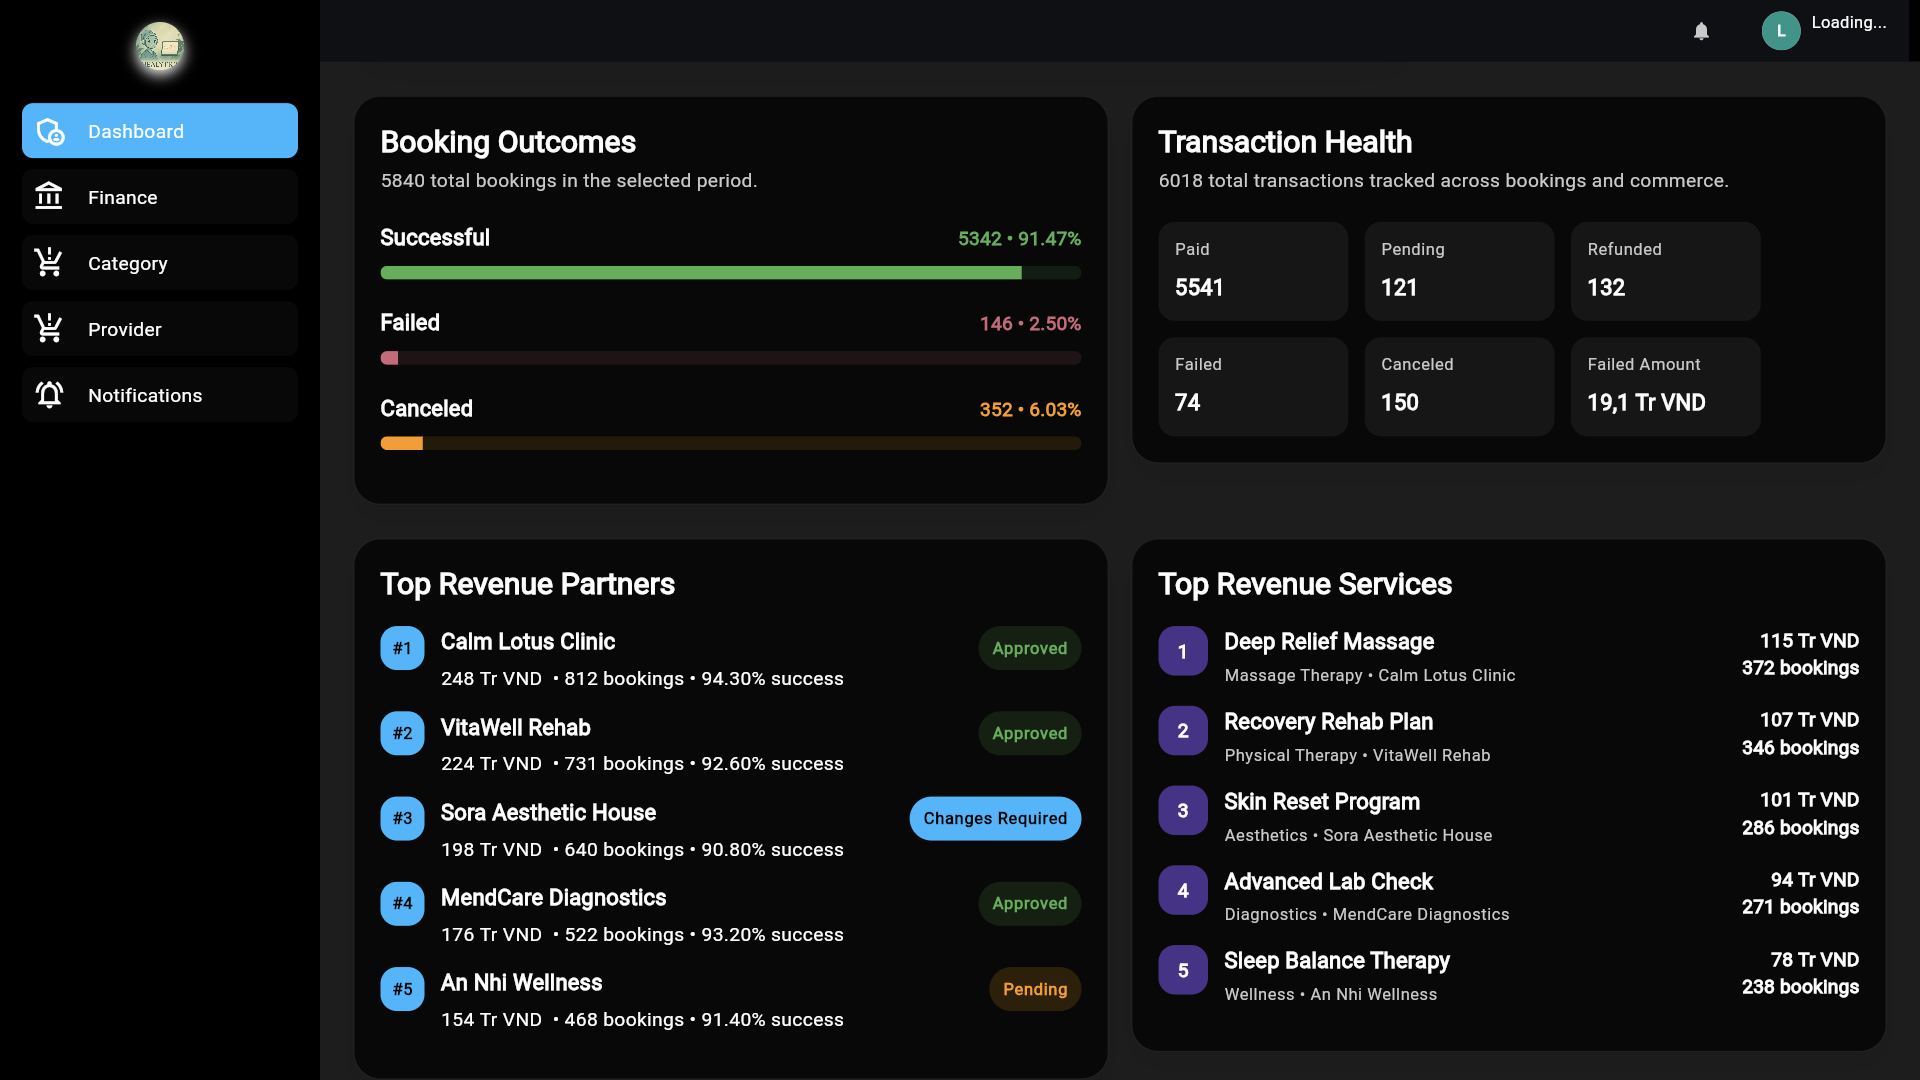
\includegraphics[width=0.92\textwidth]{Images/Hiện thực/admin/fig_admin_dashboard_bottom.png}
    \vspace{1em}
    \caption{Admin Dashboard -- phần dưới: Booking Outcomes và Top Revenue}
    \label{fig:admin_dashboard_bottom}
\end{figure}

Hình~\ref{fig:admin_dashboard_bottom} hiển thị phần dưới của Dashboard quản trị:
\begin{itemize}
    \item \textbf{Booking Outcomes:} Phân tích chi tiết trạng thái của các lượt đặt lịch (Successful, Failed, Canceled).
    \item \textbf{Transaction Health:} Thống kê tình trạng sức khỏe của các giao dịch trên hệ thống.
    \item \textbf{Bảng xếp hạng (Leaderboards):} Liệt kê Top Revenue Partners (5 đối tác có doanh thu cao nhất) và Top Revenue Services (5 dịch vụ bán chạy nhất).
\end{itemize}

\begin{figure}[H]
    \centering
    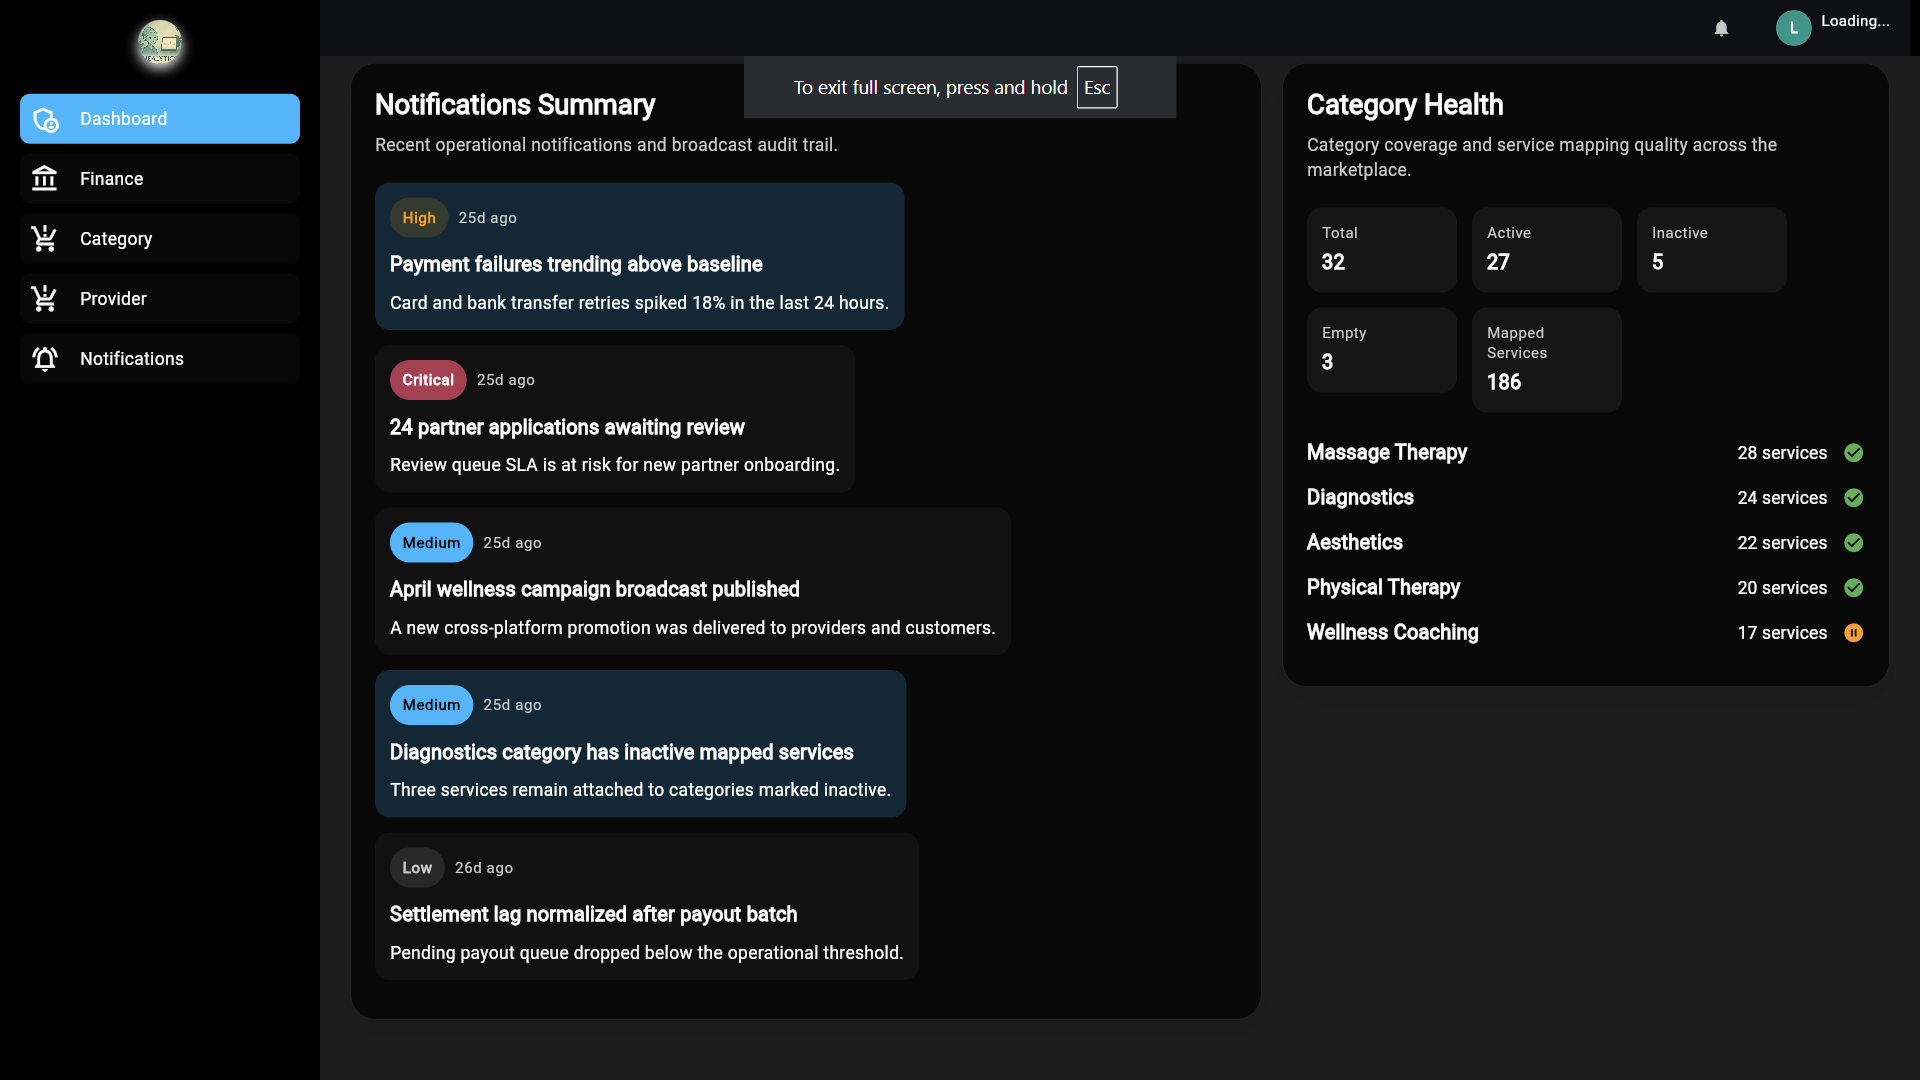
\includegraphics[width=0.92\textwidth]{Images/Hiện thực/admin/fig_admin_dashboard_notifications.png}
    \vspace{1em}
    \caption{Admin Dashboard -- khối cảnh báo và thông báo vận hành}
    \label{fig:admin_dashboard_notifications}
\end{figure}

\begin{itemize}
    \item \textbf{Thao tác giám sát:} Quản trị viên theo dõi cảnh báo quan trọng và sự kiện vận hành theo thời gian thực.
    \item \textbf{Thao tác xử lý nhanh:} Truy cập nhanh vào module liên quan để xử lý giao dịch lỗi hoặc thông báo khẩn.
\end{itemize}

Tab Overview hiển thị 8 KPI tài chính chính: Gross Volume, Net Revenue, Platform Fees, Refund Exposure, Failed Payments, Pending Payouts, Held Payouts, và Unreconciled --- mỗi chỉ số kèm tỷ lệ thay đổi so với kỳ trước. Bên dưới là bảng Revenue Trend theo ngày (Gross/Net/Refunds/Payouts) và hệ thống bộ lọc đa chiều.

\begin{figure}[H]
    \centering
    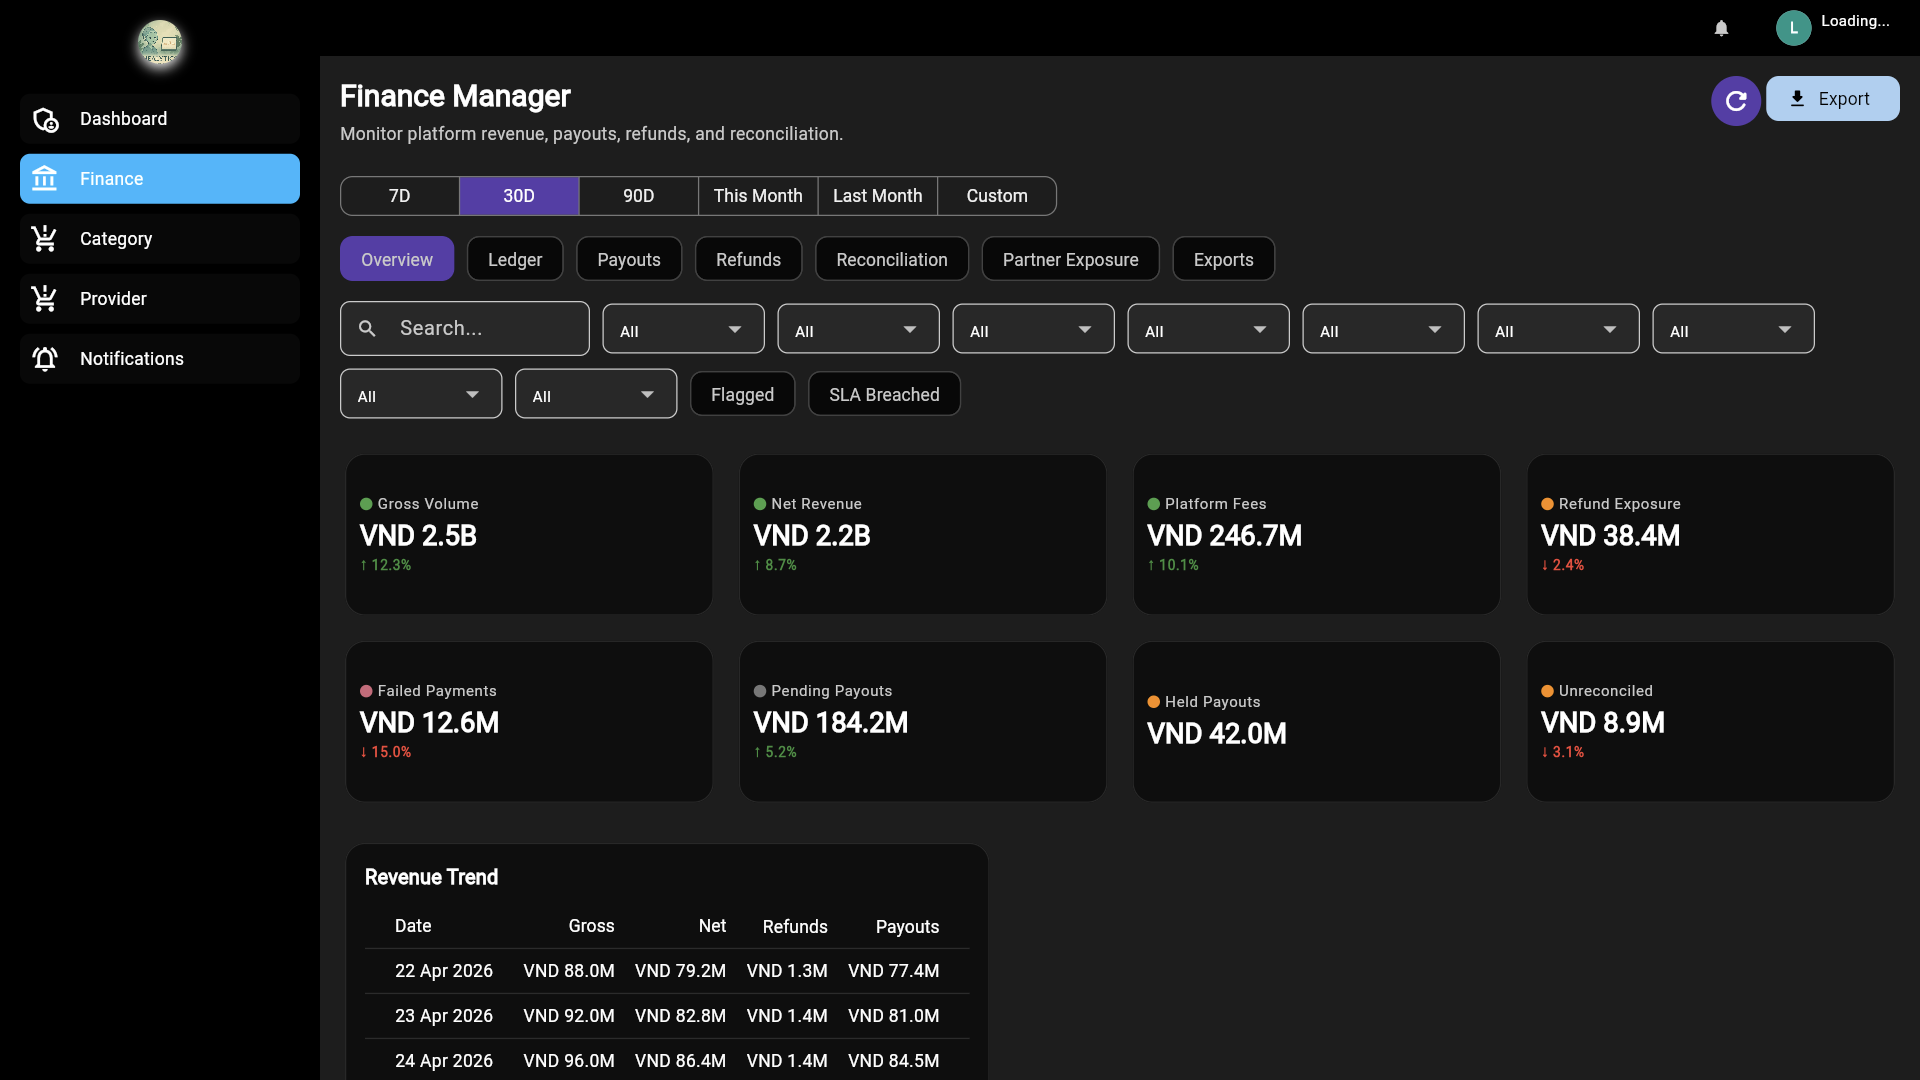
\includegraphics[width=0.85\textwidth]{Images/Hiện thực/admin/fig_admin_finance_overview.png}
    \vspace{1em}
    \caption{Finance Manager -- Tab Overview}
    \label{fig:admin_finance}
\end{figure}

\begin{figure}[H]
    \centering
    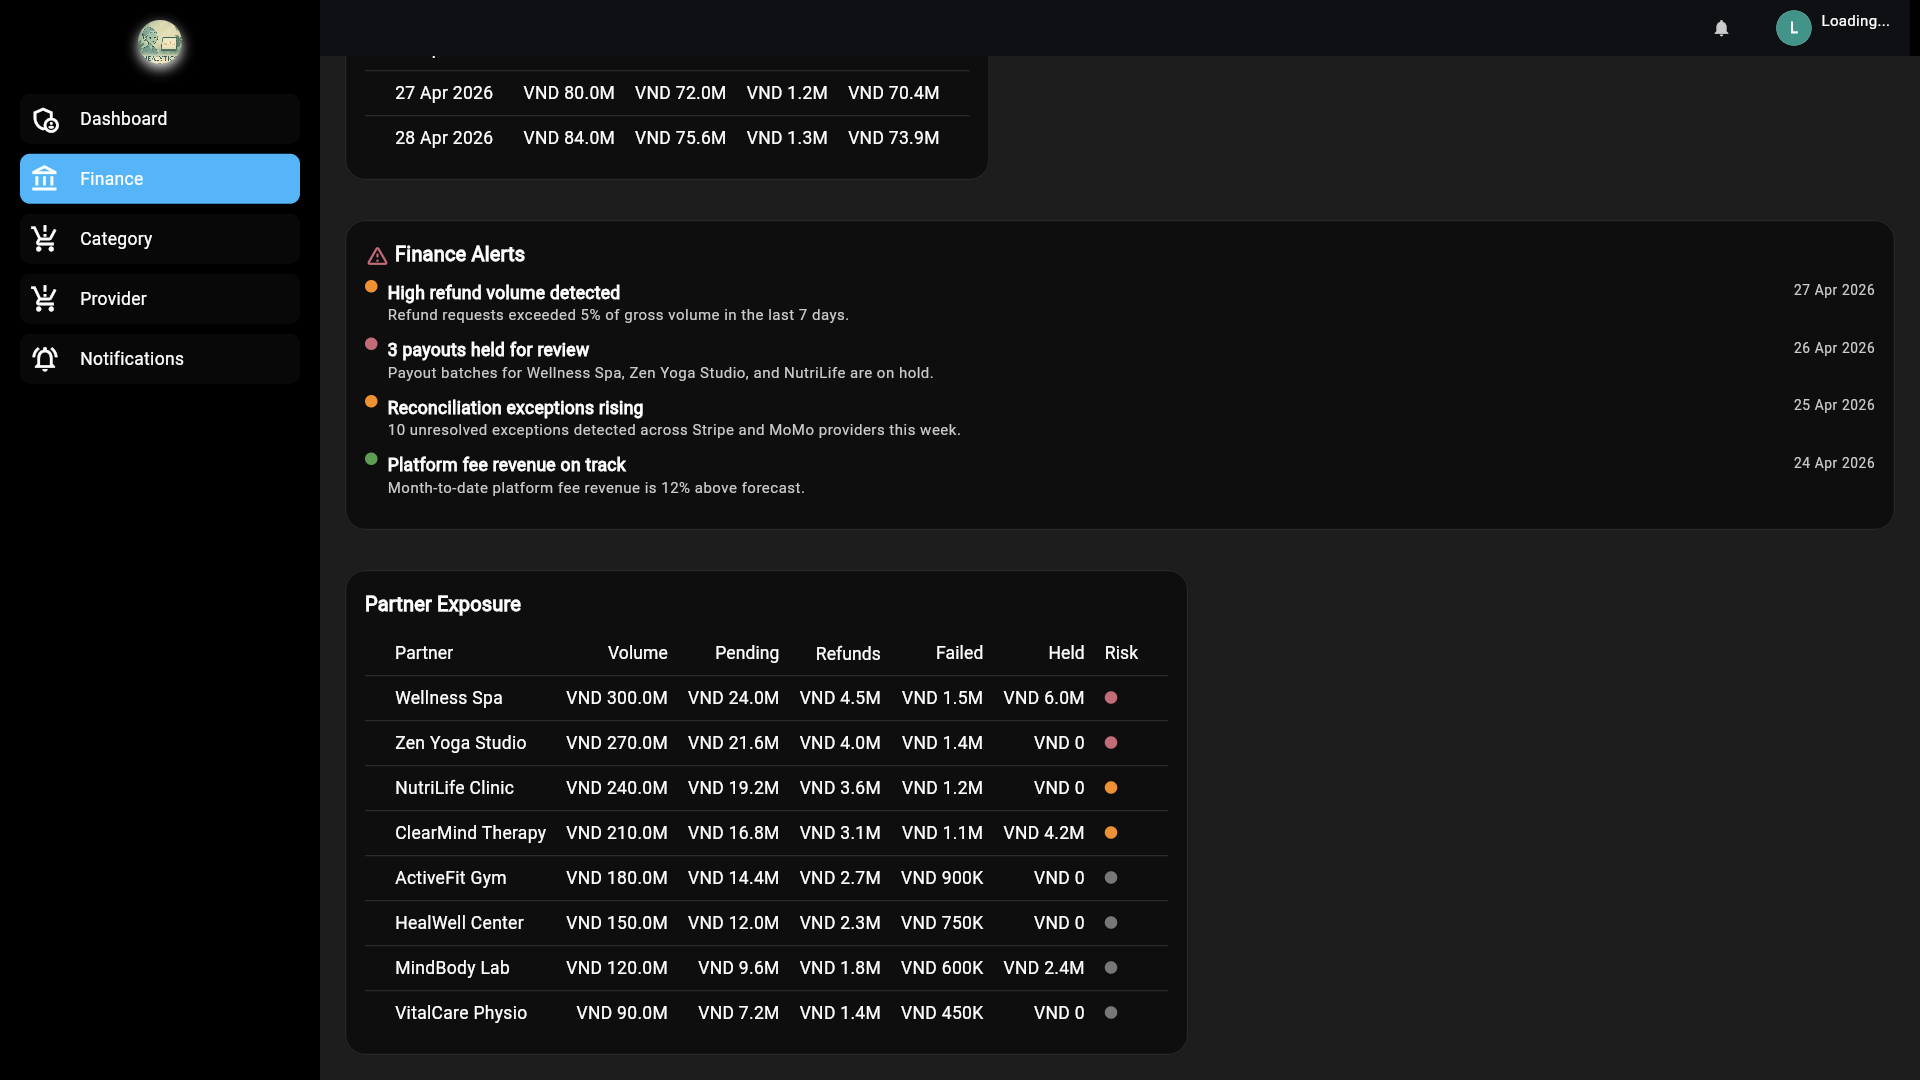
\includegraphics[width=0.85\textwidth]{Images/Hiện thực/admin/fig_admin_finance_revenue.png}
    \vspace{1em}
    \caption{Finance Manager -- Tab Revenue Trend chi tiết}
    \label{fig:admin_finance_revenue}
\end{figure}

Hình~\ref{fig:admin_finance} hiển thị tab Overview của module quản lý tài chính:
\begin{itemize}
    \item \textbf{KPI tài chính (8 chỉ số):} Bao gồm Gross Volume, Net Revenue, Platform Fees, Refund Exposure, Failed Payments, Pending Payouts, Held Payouts, và Unreconciled. Mỗi chỉ số đều kèm theo tỷ lệ thay đổi so với kỳ báo cáo trước.
    \item \textbf{Bảng Revenue Trend:} Thống kê và hiển thị chi tiết dòng tiền theo từng ngày (Gross, Net, Refunds, Payouts).
\end{itemize}

\subsubsection{Quy trình Kiểm duyệt Đối tác}

Đây là quy trình nghiệp vụ quan trọng nhất của Admin Portal. Quản trị viên thực hiện các bước sau:

\paragraph{Bước 1 -- Xem danh sách đối tác chờ duyệt}

Tại menu ``Provider'', quản trị viên thấy danh sách toàn bộ đối tác với thông tin: tên, ID, loại hình kinh doanh, ngày nộp, trạng thái (Pending/Active/Rejected), và các nút hành động. Cột ``Actions'' hiển thị nút ``Review Application'' cho các hồ sơ đang chờ duyệt (Hình~\ref{fig:admin_provider_list}).

\begin{figure}[H]
    \centering
    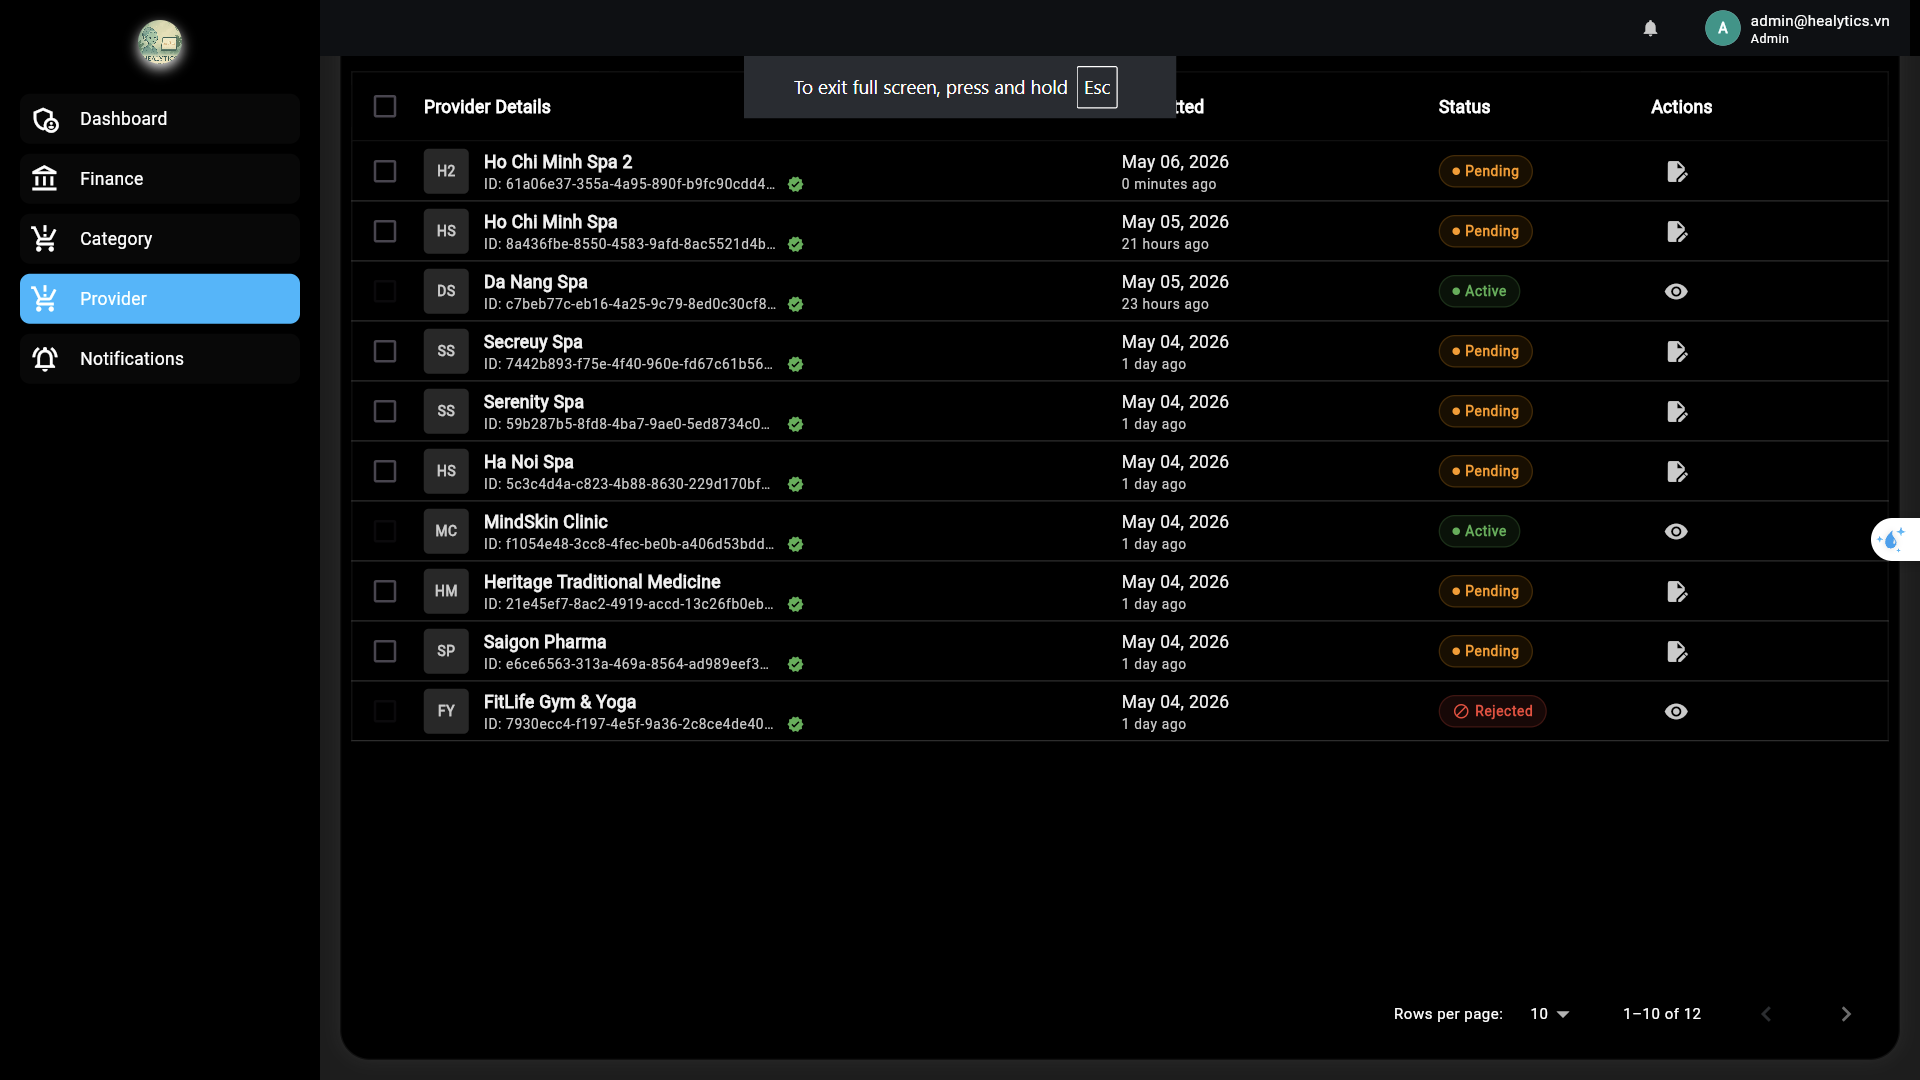
\includegraphics[width=0.85\textwidth]{Images/Hiện thực/admin/fig_admin_provider_list_new.png}
    \vspace{1em}
    \caption{Danh sách đối tác chờ duyệt tại module Provider}
    \label{fig:admin_provider_list}
\end{figure}

Hình~\ref{fig:admin_provider_list} hiển thị danh sách toàn bộ đối tác:
\begin{itemize}
    \item \textbf{Thông tin hiển thị:} Tên đối tác, ID, loại hình kinh doanh, ngày nộp hồ sơ, và trạng thái hiện tại (Pending/Active/Rejected).
    \item \textbf{Cột Actions (Hành động):} Cung cấp nút ``Review Application'' (hiển thị màu xanh khi hover) cho phép quản trị viên truy cập nhanh vào các hồ sơ đang trong trạng thái chờ duyệt.
\end{itemize}

\paragraph{Bước 2 -- Xem chi tiết và xét duyệt từng trường}

Khi nhấn ``Review Application'', quản trị viên được chuyển đến trang chi tiết hồ sơ (Hình~\ref{fig:admin_detail_top} và Hình~\ref{fig:admin_detail_bottom}) gồm:

\begin{itemize}
    \item \textbf{Business Overview:} Tên thương hiệu, mã số thuế, loại hình, địa chỉ (hiển thị trên bản đồ), và đường dẫn.
    \item \textbf{Account \& Contact:} Email và số điện thoại liên hệ.
    \item \textbf{Legal Representative:} Họ tên, chức vụ, loại giấy tờ, số giấy tờ, ngày cấp.
    \item \textbf{KYC Documents (cột phải):} Ảnh CCCD mặt trước/sau (có nút zoom), Giấy phép kinh doanh (có nút tải xuống).
\end{itemize}

Mỗi trường có biểu tượng \checkmark{} (hợp lệ) và \textit{bút chỉnh sửa} (cần sửa). Khi admin đánh dấu một trường cần sửa, hệ thống hiển thị popup ``Revision Note'' để nhập lý do cụ thể (Hình~\ref{fig:admin_revision_note}). Cuối trang, admin chọn \textbf{``Approve Provider''} (nút xanh) hoặc \textbf{``Reject Application''} (nút đỏ).

\begin{figure}[H]
    \centering
    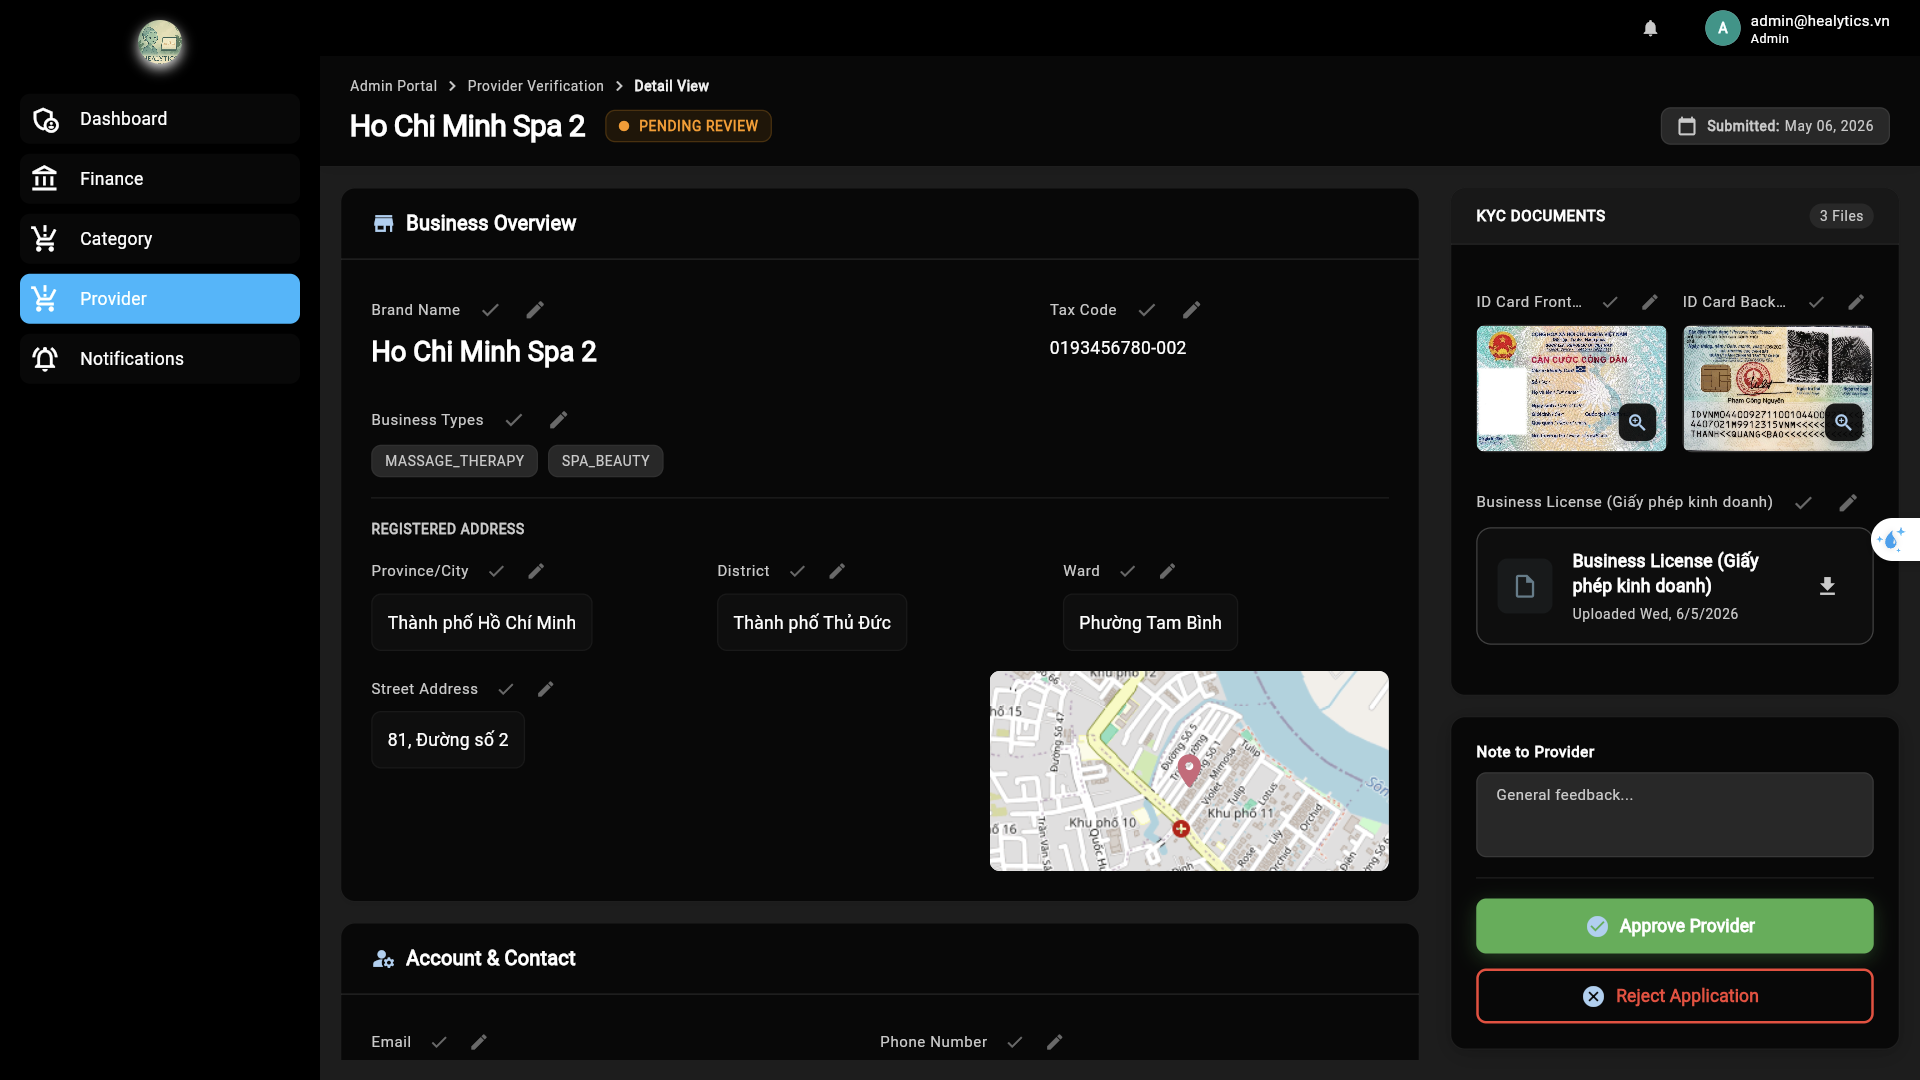
\includegraphics[width=0.92\textwidth]{Images/Hiện thực/admin/fig_admin_provider_detail_top.png}
    \vspace{1em}
    \caption{Trang xét duyệt đối tác -- phần trên: Business Overview và KYC Documents}
    \label{fig:admin_detail_top}
\end{figure}

Hình~\ref{fig:admin_detail_top} hiển thị phần trên của trang chi tiết xét duyệt hồ sơ:
\begin{itemize}
    \item \textbf{Ngữ cảnh \& Trạng thái:} Sử dụng breadcrumb ``Provider Verification > Detail View'' và tiêu đề kèm badge \textbf{PENDING REVIEW} cùng ngày nộp hồ sơ.
    \item \textbf{Business Overview:} Liệt kê Brand Name, Tax Code, Business Types, và Registered Address (được trực quan hóa trên bản đồ Google Maps).
    \item \textbf{KYC Documents (cột phải):} Hiển thị ảnh CCCD mặt trước/sau (có tính năng phóng to) và Giấy phép kinh doanh (có tính năng tải xuống).
    \item \textbf{Công cụ đánh giá:} Mỗi trường thông tin đều kèm biểu tượng \checkmark{} (đánh dấu hợp lệ) và biểu tượng bút chỉnh sửa (đánh dấu có lỗi).
\end{itemize}

\begin{figure}[H]
    \centering
    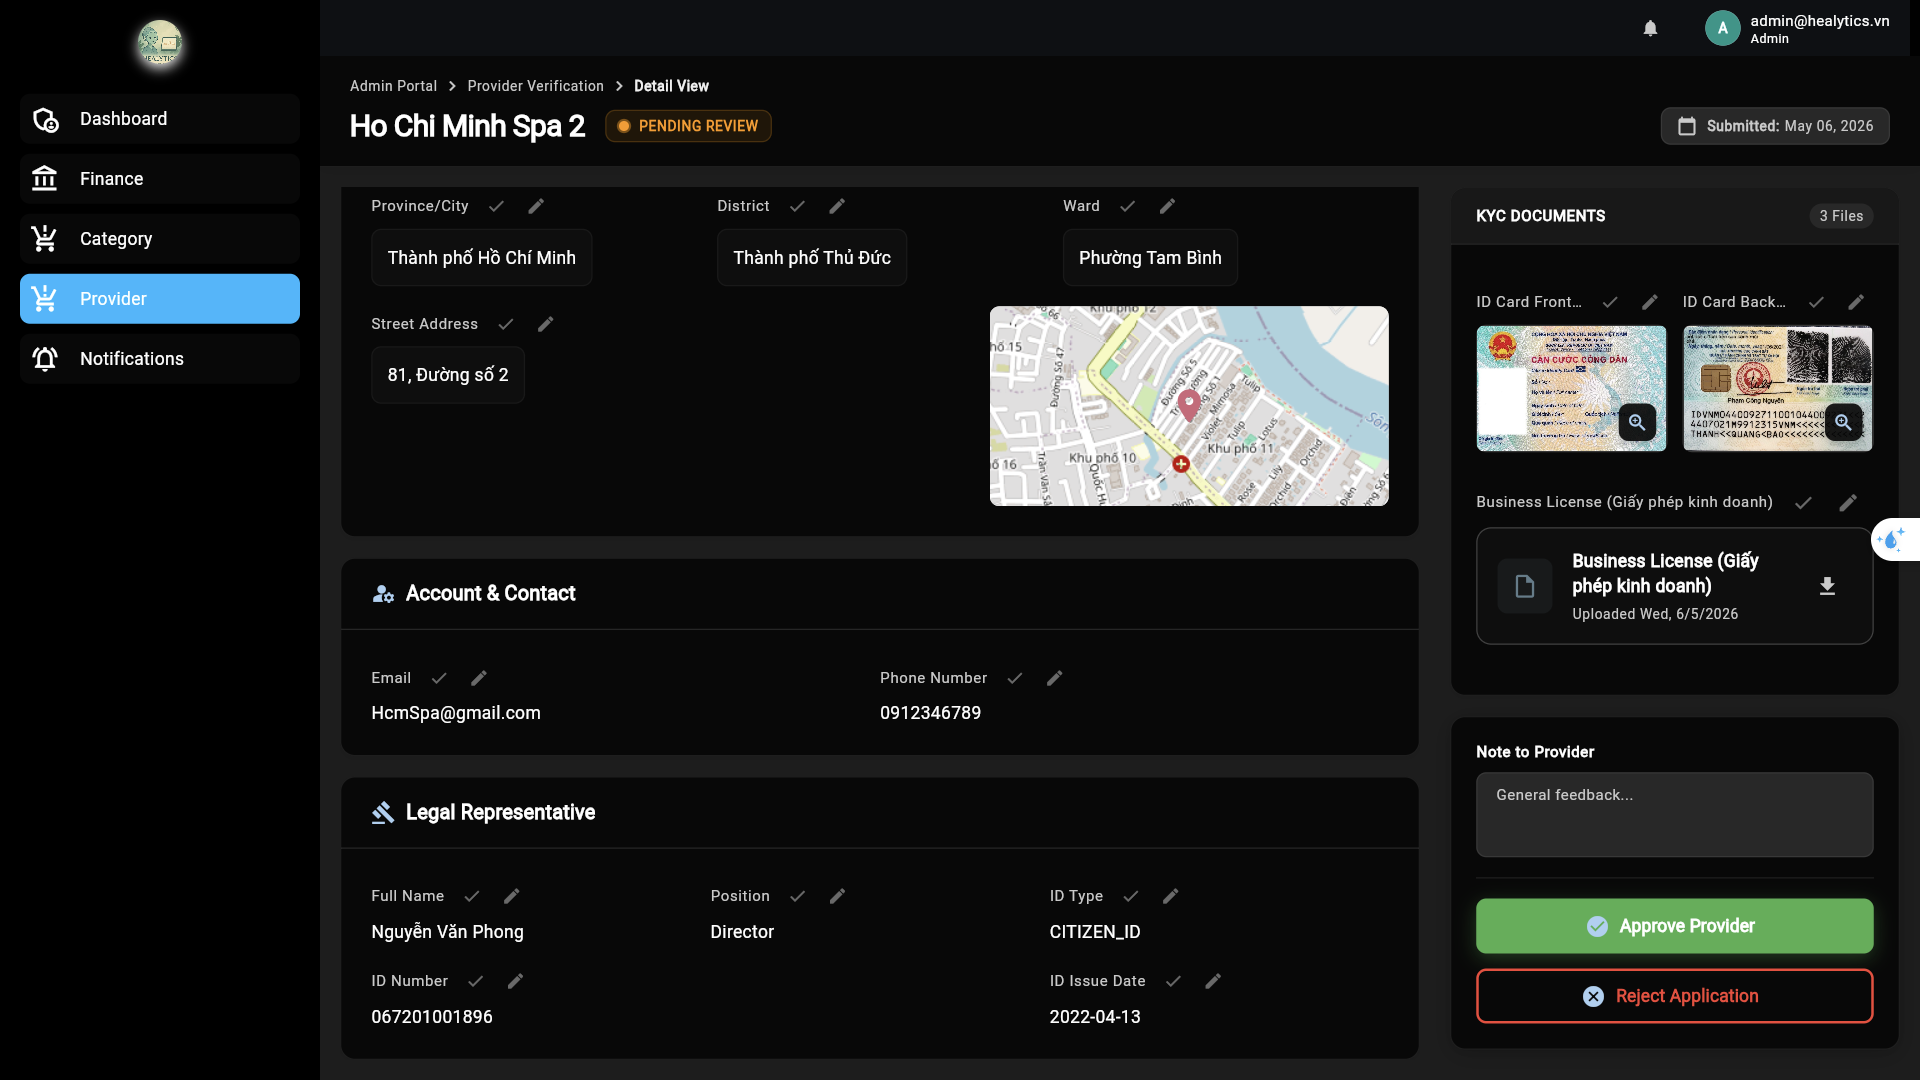
\includegraphics[width=0.92\textwidth]{Images/Hiện thực/admin/fig_admin_provider_detail_bottom.png}
    \vspace{1em}
    \caption{Trang xét duyệt đối tác -- phần dưới: Contact, Legal Representative và nút hành động}
    \label{fig:admin_detail_bottom}
\end{figure}

Hình~\ref{fig:admin_detail_bottom} hiển thị phần dưới của trang chi tiết xét duyệt hồ sơ:
\begin{itemize}
    \item \textbf{Thông tin chi tiết:} Bao gồm phần \textbf{Account \& Contact} (Email, Phone) và phần \textbf{Legal Representative} (Full Name, Position, ID Type, ID Number, ID Issue Date).
    \item \textbf{Hành động xét duyệt:} Cung cấp hai nút quyết định chính là \textbf{``Approve Provider''} (chấp thuận - nút xanh) và \textbf{``Reject Application''} (từ chối - nút đỏ).
    \item \textbf{Phản hồi chung:} Ô \textbf{Note to Provider} cho phép quản trị viên nhập nhận xét và hướng dẫn tổng thể cho đối tác.
\end{itemize}

% Hình bản đồ Business Overview -- tạm comment vì nội dung trùng với Hình admin_detail_top
% \begin{figure}[H]
%     \centering
%     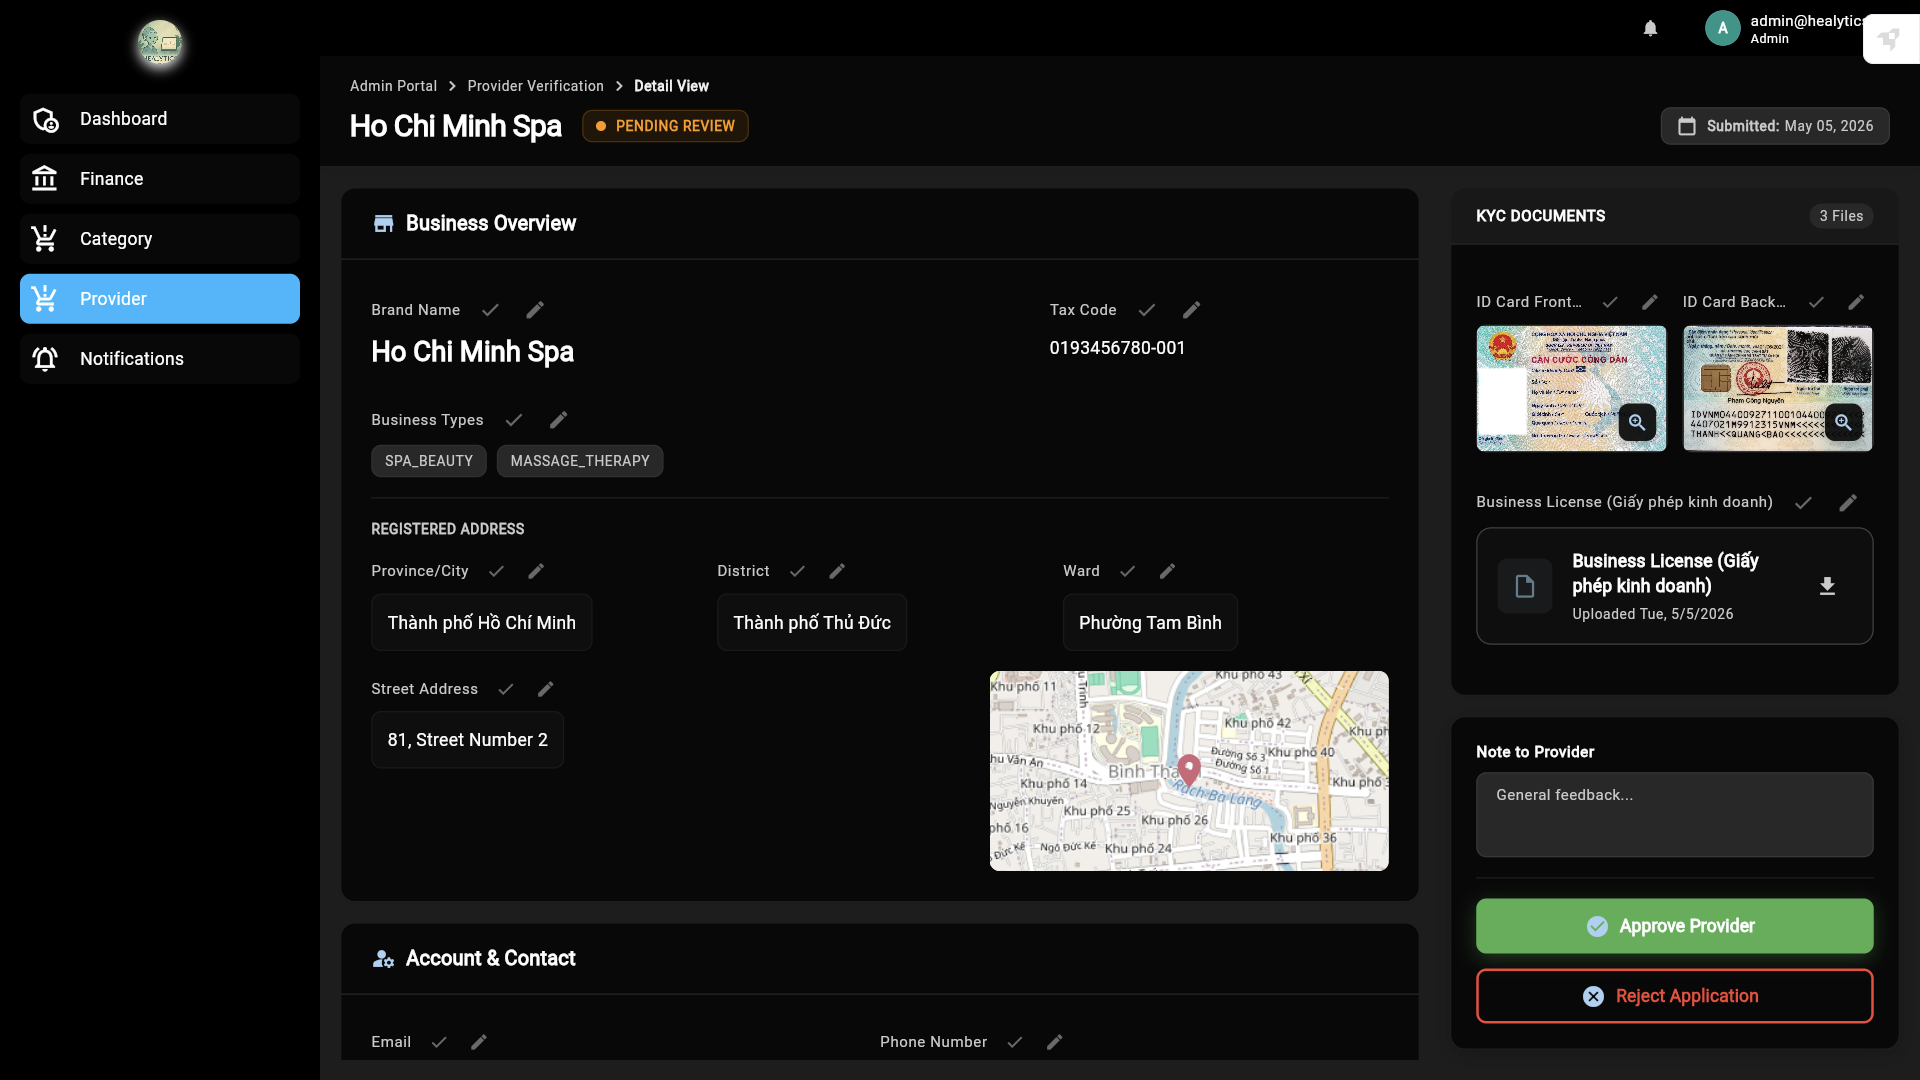
\includegraphics[width=0.92\textwidth]{Images/Hiện thực/admin/fig_admin_verify_business_top.png}
%     \caption{Business Overview -- bản đồ vị trí kinh doanh}
%     \label{fig:admin_verify_map}
% \end{figure}

\begin{figure}[H]
    \centering
    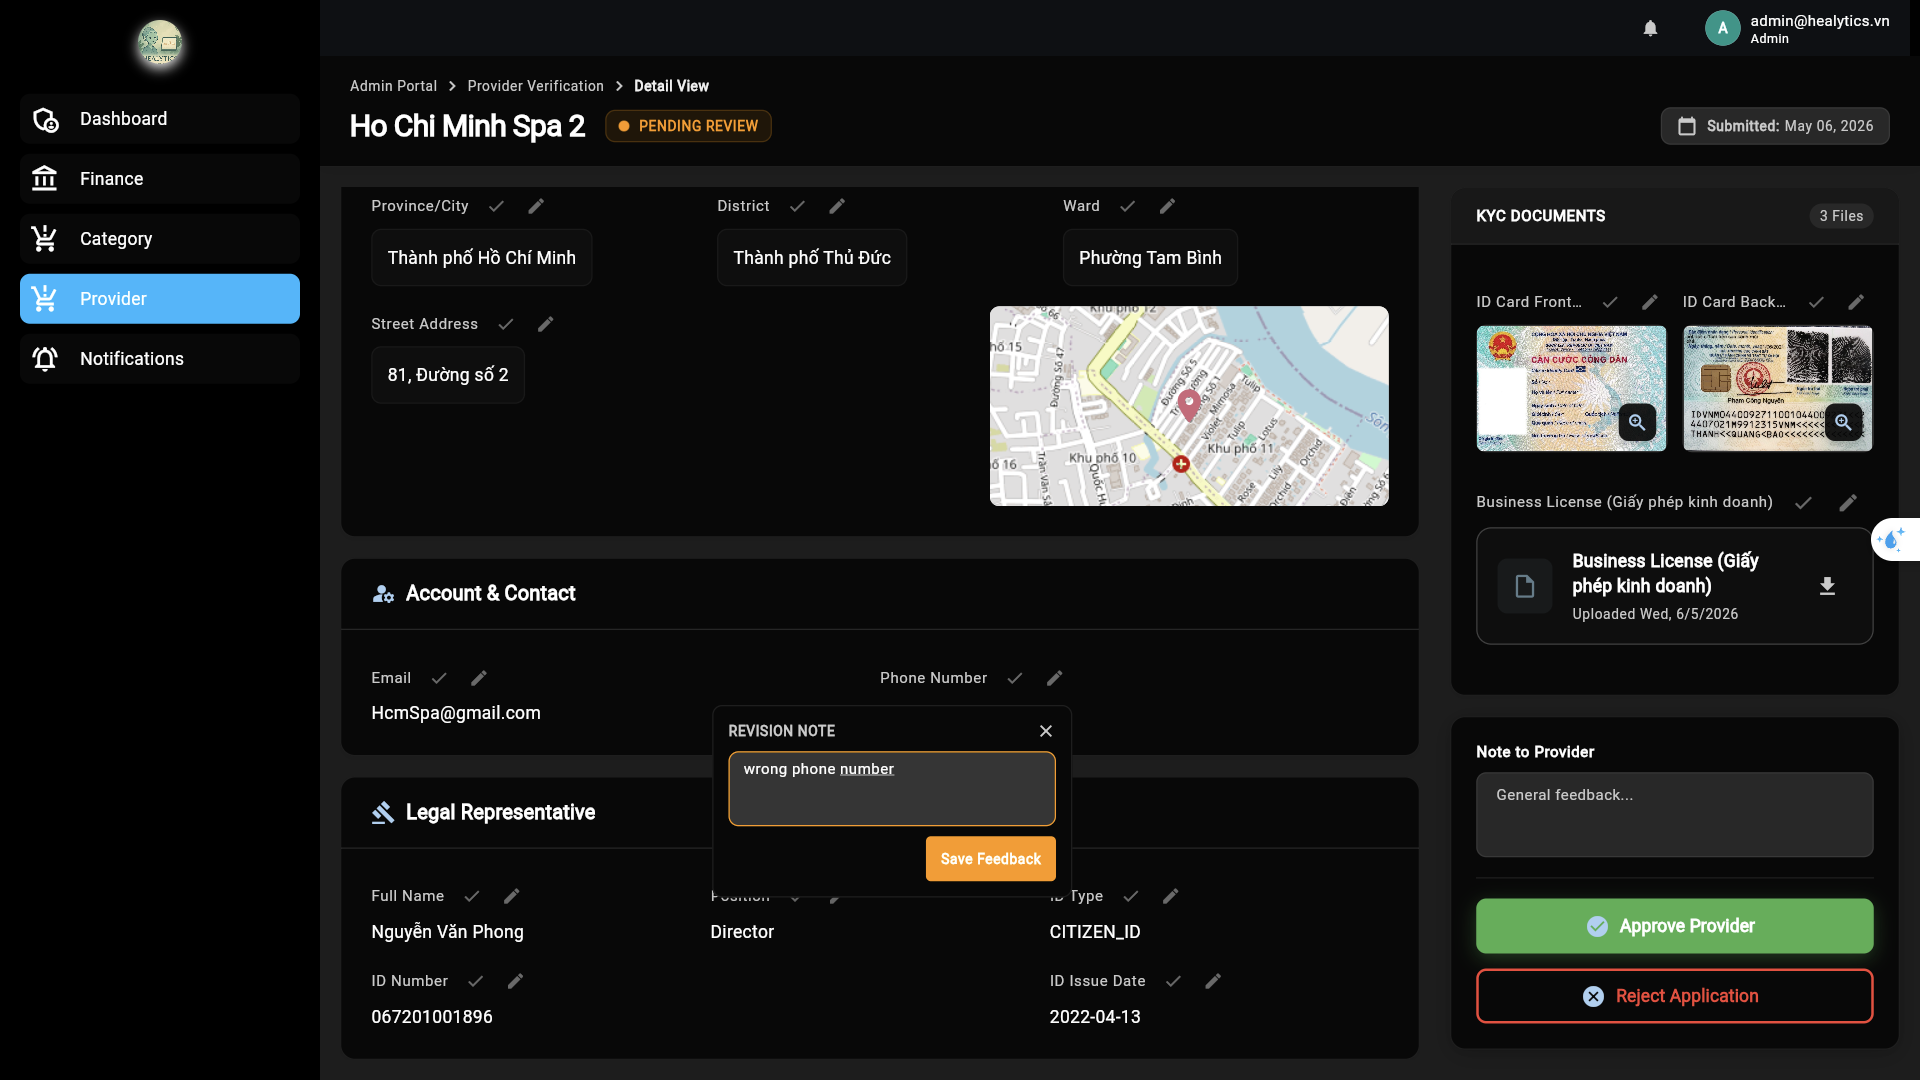
\includegraphics[width=0.92\textwidth]{Images/Hiện thực/admin/fig_admin_provider_revision_note.png}
    \vspace{1em}
    \caption{Popup Revision Note khi đánh dấu trường cần sửa}
    \label{fig:admin_revision_note}
\end{figure}

Hình~\ref{fig:admin_revision_note} hiển thị tính năng ghi chú yêu cầu chỉnh sửa:
\begin{itemize}
    \item \textbf{Popup Revision Note:} Xuất hiện khi quản trị viên nhấn vào biểu tượng bút chỉnh sửa bên cạnh bất kỳ một trường thông tin nào.
    \item \textbf{Nhập lý do:} Quản trị viên nhập phản hồi lỗi cụ thể (ví dụ: ``wrong phone number'') và xác nhận.
    \item \textbf{Hiển thị phản hồi:} Ghi chú này sẽ được đồng bộ và hiển thị trực tiếp trên giao diện của đối tác để hướng dẫn họ cập nhật lại thông tin một cách chính xác.
\end{itemize}

\paragraph{Logic xét duyệt phía Backend}

Khi quản trị viên xét duyệt một hồ sơ đối tác, hệ thống xử lý theo các bước:

\begin{enumerate}
    \item \textbf{Kiểm tra điều kiện:} Chỉ cho phép xét duyệt khi đối tác đang ở trạng thái \texttt{PENDING}. Nếu không, hệ thống trả về lỗi.

    \item \textbf{Phân loại đánh giá:} Quản trị viên gửi danh sách các mục cần đánh giá, mỗi mục gồm \texttt{fieldKey} và \texttt{feedback}. Hệ thống tự động phân loại thành đánh giá trường hồ sơ hoặc đánh giá tài liệu dựa trên danh sách trường đã biết.

    \item \textbf{Lưu ảnh chụp dữ liệu (Snapshot):} Với mỗi mục được đánh giá, hệ thống lưu lại giá trị hiện tại kèm kết quả hợp lệ hay không và phản hồi chi tiết, giúp truy vết chính xác dữ liệu tại thời điểm xét duyệt.

    \item \textbf{Xác định kết quả cuối cùng:} Hệ thống áp dụng quy tắc ưu tiên:
    \begin{itemize}
        \item Nếu quản trị viên chọn từ chối $\rightarrow$ \texttt{REJECTED} (ưu tiên cao nhất, không thể đảo ngược).
        \item Nếu có bất kỳ mục nào bị đánh dấu lỗi $\rightarrow$ \texttt{REQUIRED\_RESUBMIT} (yêu cầu sửa lại).
        \item Nếu tất cả hợp lệ và đủ tài liệu bắt buộc $\rightarrow$ \texttt{APPROVED}.
    \end{itemize}

    \item \textbf{Ghi nhận lịch sử:} Toàn bộ kết quả xét duyệt được lưu vào bảng \texttt{PartnerReviewLog} dưới dạng bản ghi bất biến (immutable), bao gồm: kết quả, người duyệt, nhận xét chung, và chi tiết đánh giá từng trường/tài liệu.
\end{enumerate}

\subsubsection{Quản lý Danh mục và Thông báo}

\paragraph{Module Danh mục (Category)}

\begin{figure}[H]
    \centering
    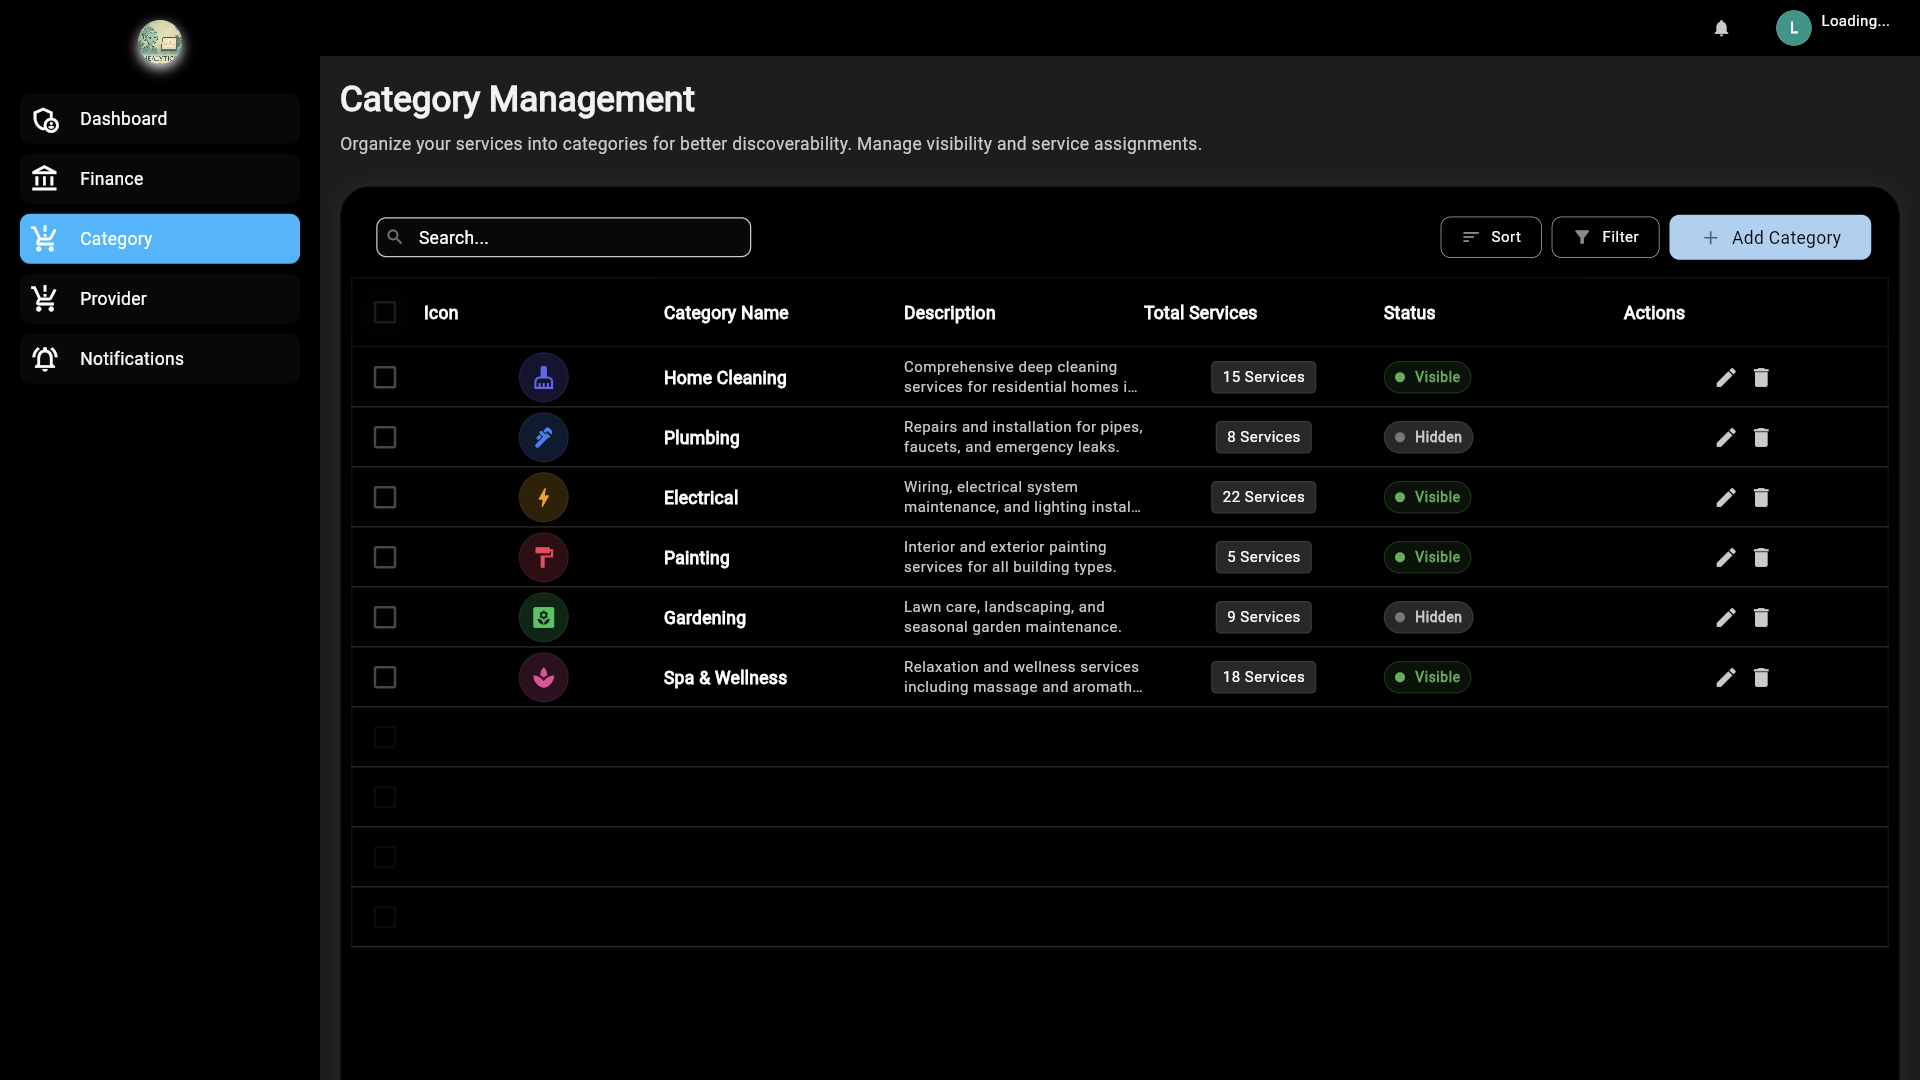
\includegraphics[width=0.92\textwidth]{Images/Hiện thực/admin/fig_admin_category.png}
    \vspace{1em}
    \caption{Giao diện Category Management}
    \label{fig:admin_category}
\end{figure}

Hình~\ref{fig:admin_category} hiển thị giao diện quản lý danh mục dịch vụ:
\begin{itemize}
    \item \textbf{Thông tin hiển thị:} Bao gồm các cột Name, Slug, Icon, Description, Status (Active/Inactive), Services (số lượng dịch vụ đang liên kết), và Created At.
    \item \textbf{Thao tác quản trị:} Cho phép quản trị viên thực hiện tạo mới, chỉnh sửa nội tuyến (inline editing), hoặc chuyển đổi trạng thái hiển thị của từng danh mục.
\end{itemize}

\paragraph{Module Thông báo (Notification Control Center)}

\begin{figure}[H]
    \centering
    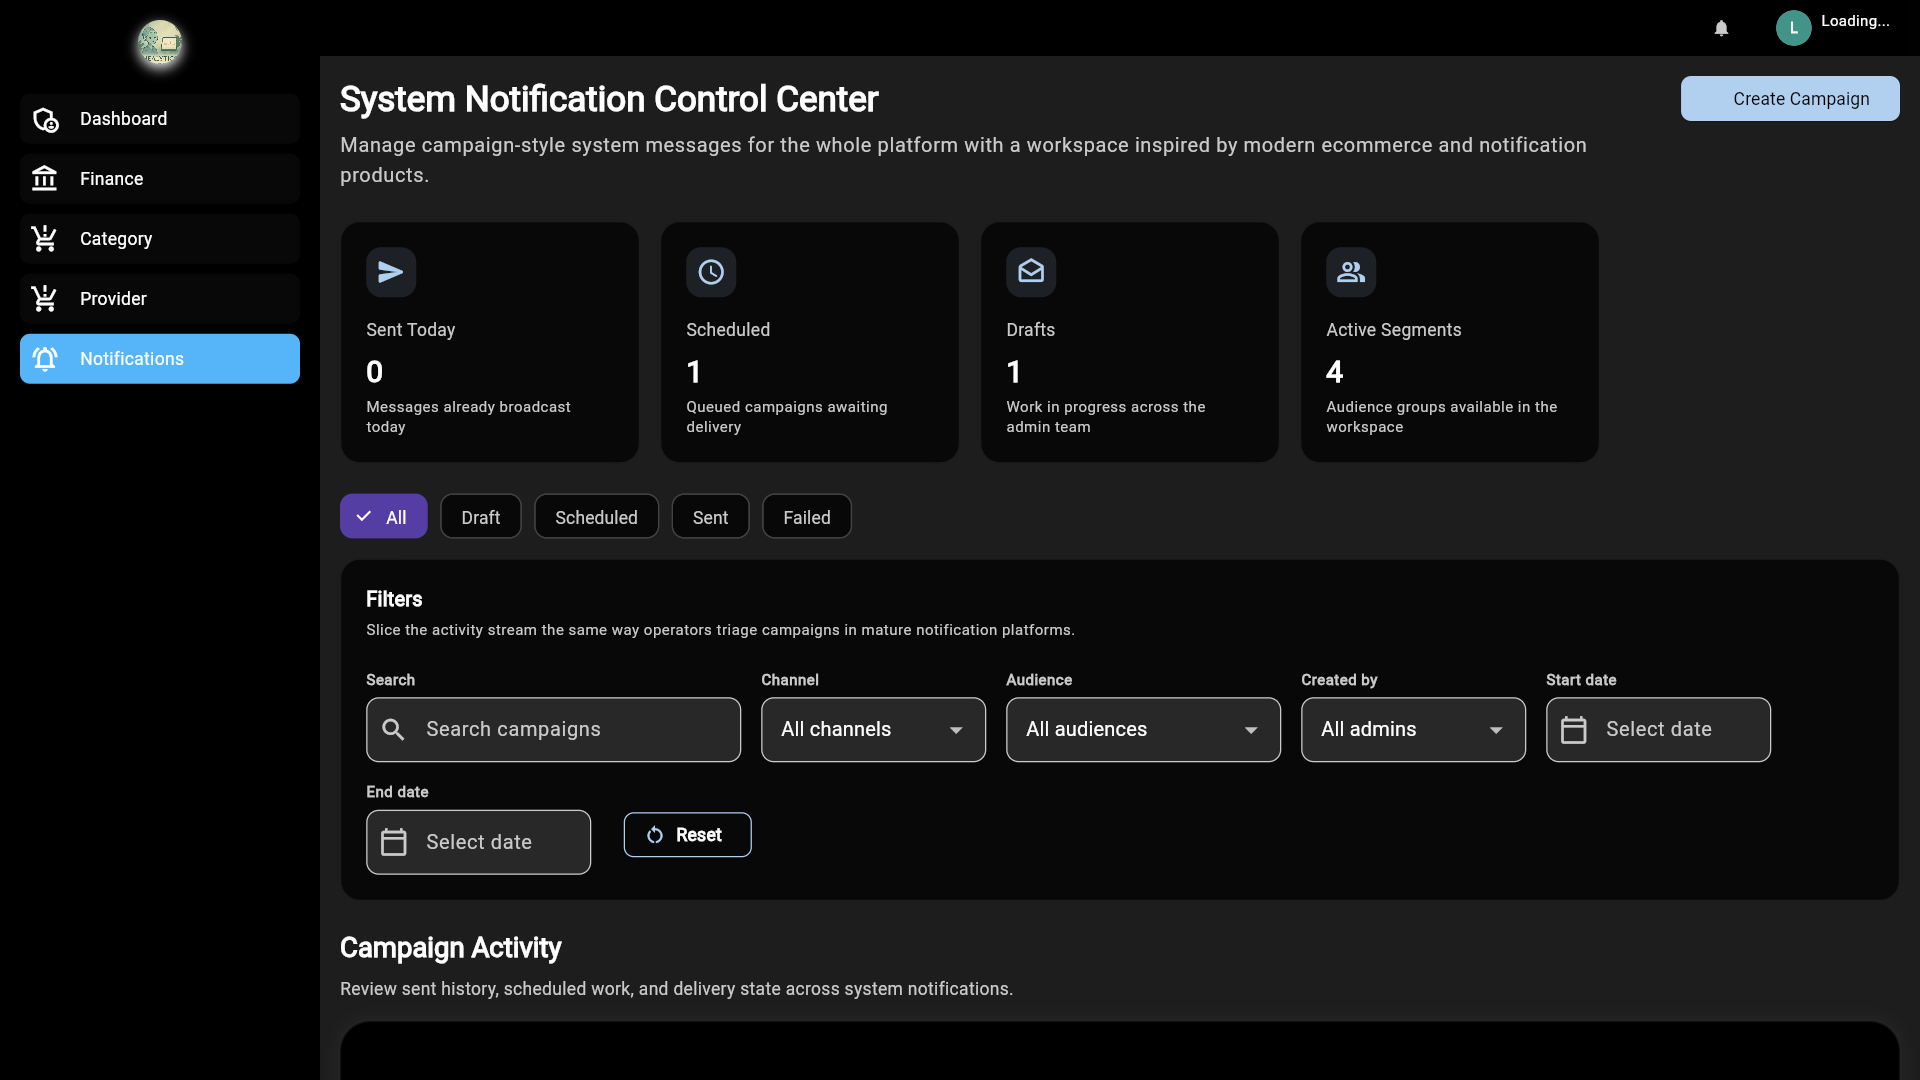
\includegraphics[width=0.92\textwidth]{Images/Hiện thực/admin/fig_admin_notification_center.png}
    \vspace{1em}
    \caption{Giao diện Notification Control Center}
    \label{fig:admin_notification}
\end{figure}

\begin{figure}[H]
    \centering
    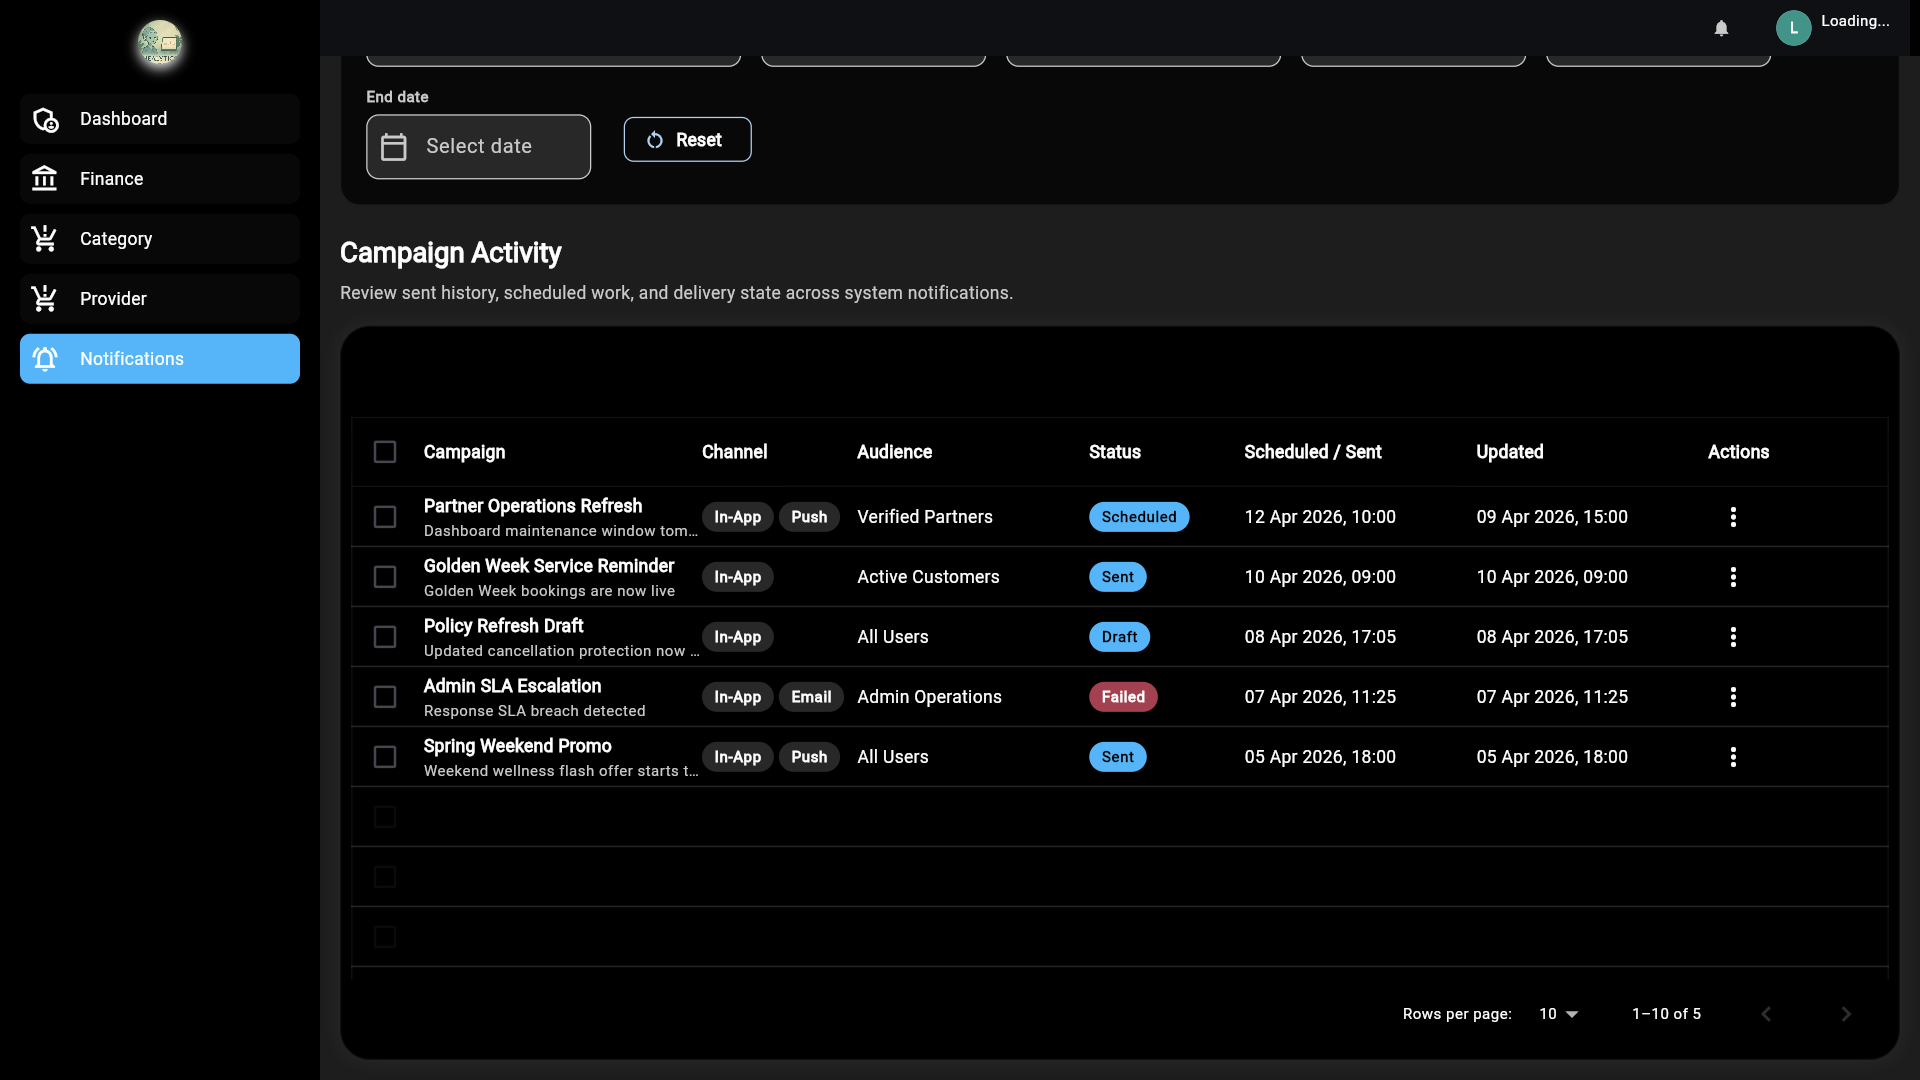
\includegraphics[width=0.92\textwidth]{Images/Hiện thực/admin/fig_admin_notification_campaigns.png}
    \vspace{1em}
    \caption{Notification Control Center -- màn hình quản lý chiến dịch}
    \label{fig:admin_notification_campaigns}
\end{figure}

Hình~\ref{fig:admin_notification} hiển thị Notification Control Center (Trung tâm quản lý thông báo):
\begin{itemize}
    \item \textbf{Tạo chiến dịch:} Cho phép quản trị viên soạn thảo và cấu hình các chiến dịch thông báo broadcast gửi đến những nhóm đối tượng mục tiêu cụ thể.
    \item \textbf{Theo dõi trạng thái:} Cung cấp trạng thái thời gian thực của các thông báo (Draft, Sent, Scheduled, Failed).
    \item \textbf{Phân tích hiệu quả:} Hiển thị các chỉ số tương tác quan trọng như Delivery rates (tỷ lệ gửi thành công), Open rates (tỷ lệ mở), và Click rates (tỷ lệ nhấp chuột).
\end{itemize}

\subsubsection{Nhật ký Kiểm toán (Audit Logging)}

Ngoài lịch sử xét duyệt, hệ thống còn ghi lại mọi thao tác quan trọng của quản trị viên thông qua module \texttt{AuditModule}:

\begin{itemize}
    \item \textbf{Đánh dấu hành động:} Sử dụng decorator \texttt{@Audit} gắn trực tiếp trên các API cần theo dõi, ví dụ: \texttt{@Audit('PARTNER\_REVIEW', 'Partner')}.
    \item \textbf{Tự động ghi nhận:} \texttt{AuditInterceptor} tự động thu thập thông tin trước và sau khi API được thực thi, bao gồm: ai thực hiện, thao tác gì, tác động đến đối tượng nào, và thời điểm cụ thể.
    \item \textbf{Tra cứu linh hoạt:} \texttt{AuditService} cho phép tìm kiếm nhật ký theo người thực hiện, đối tượng bị tác động, hoặc loại hành động.
\end{itemize}

Nhờ kết hợp giữa \texttt{PartnerReviewLog} và \texttt{AuditLog}, hệ thống đảm bảo khả năng truy vết toàn diện: ai đã duyệt hồ sơ nào, vào lúc nào, và dữ liệu lúc đó trông ra sao.



\section{Hiện thực và Tích hợp các dịch vụ Trí tuệ Nhân tạo (AI Services)}
\subsection{Hiện thực dịch vụ nhận dạng thực thể (NER Service)}


\subsubsection{Kiến trúc Hybrid NER và quyết định thiết kế}

Hệ thống dùng kiến trúc \textbf{Hybrid NER}, kết hợp ba lớp xử lý bổ trợ nhau:
\begin{itemize}
    \item \textbf{LLM extraction (Gemini):} xử lý các thực thể ngữ nghĩa trong \texttt{gemini\_ner.py}, với model mặc định \texttt{gemini-2.5-flash}.
    \item \textbf{Rule-based extraction (Regex):} xử lý các mẫu định lượng và làm lớp dự phòng trong \texttt{extractor.py} và \texttt{distance\_extractor.py}.
    \item \textbf{Fallback nội bộ:} kết hợp \texttt{underthesea}, keyword scan và bộ so khớp địa danh (Aho-Corasick hoặc n-gram fallback) trong \texttt{extractor.py}.
\end{itemize}

Các tham số cấu hình chính nằm trong \texttt{config.py}:
\begin{itemize}
    \item \texttt{QUERY\_CACHE\_MAXSIZE = 1000}.
    \item \texttt{LOCATION\_CACHE\_TTL = 3600} giây.
    \item \texttt{GEMINI\_TIMEOUT\_MS = 1500}, \texttt{GEMINI\_MAX\_RETRIES = 1}, \texttt{GEMINI\_COOLDOWN\_SECONDS = 5}.
    \item \texttt{NER\_MIN\_CONFIDENCE = 0.8} cho lọc \texttt{BUSINESS\_TYPE}.
    \item \texttt{DEFAULT\_PROXIMITY\_RADIUS\_M = 10000}, \texttt{MAX\_PROXIMITY\_RADIUS\_M = 50000}.
\end{itemize}


\subsubsection{Pipeline xử lý truy vấn}

Khi nhận truy vấn tự nhiên, NER Service xử lý theo pipeline tuần tự:
\begin{enumerate}
    \item \textbf{Hybrid extraction} (\texttt{extractor.py}): nhận thực thể từ Gemini rồi bổ sung bằng underthesea, keyword và location fallback.
    \item \textbf{Numeric policy} (\texttt{extractor.py}): \texttt{PRICE} và \texttt{DISTANCE} dùng hướng \textit{Gemini-first}; khi Gemini không trả kết quả thì mới rơi về parser cục bộ.
    \item \textbf{Entity normalization} (\texttt{normalizer.py}): quy đổi về schema chuẩn gồm \texttt{business\_type}, \texttt{location\_code}, \texttt{operator}, \texttt{amount}.
    \item \textbf{Spatial resolution} (\texttt{spatial\_context.py}): xử lý ngữ cảnh khoảng cách và tọa độ người dùng.
    \item \textbf{Pre-filter query} (\texttt{query\_builder.py}, \texttt{db\_fetcher.py}): dựng điều kiện truy vấn và lấy ứng viên từ DB/PostGIS.
\end{enumerate}

Đầu ra endpoint:
\begin{itemize}
    \item \texttt{/ner/extract}: trả \texttt{NerResponse} (entities + \texttt{extraction\_source}) trong \texttt{ner\_routes.py}.
    \item \texttt{/prefilter/search}: trả \textbf{List[String]} (danh sách \texttt{service\_id}) trong \texttt{prefilter\_routes.py}.
\end{itemize}

\subsubsection{Tối ưu hiệu năng và độ bền vận hành}

NER Service có một số cơ chế tối ưu quan trọng để giữ độ trễ ổn định trong môi trường thời gian thực:
\begin{itemize}
    \item \textbf{LRU query cache:} giữ tối đa 1000 truy vấn (\texttt{QUERY\_CACHE\_MAXSIZE}) trong \texttt{extractor.py}.
    \item \textbf{Aho-Corasick location matching:} bật/tắt bằng \texttt{LOCATION\_MATCHER\_USE\_AHO}; nếu không khả dụng thì chuyển sang n-gram fallback trong \texttt{extractor.py}.
    \item \textbf{Stale-while-revalidate cho cache địa lý:} TTL 3600 giây trong \texttt{cache.py}.
    \item \textbf{Confidence gating:} ngưỡng \texttt{NER\_MIN\_CONFIDENCE = 0.8} cho \texttt{BUSINESS\_TYPE} trong \texttt{gemini\_ner.py}.
\end{itemize}

\subsubsection{Schema giao tiếp và tính xác định đầu ra}

Dữ liệu trao đổi giữa Gateway và NER Service được chuẩn hóa bằng Pydantic models. Ngoài bộ trường \texttt{type/value/confidence}, mỗi thực thể còn mang thêm thông tin ngữ nghĩa để phục vụ bước dựng truy vấn:
\begin{itemize}
    \item \texttt{business\_type} cho thực thể loại hình dịch vụ.
    \item \texttt{location\_code}, \texttt{location\_level} cho thực thể địa điểm.
    \item \texttt{operator}, \texttt{amount}, \texttt{amount\_max} cho thực thể định lượng.
\end{itemize}

Trong mã hiện thực, schema entity được định nghĩa ở \texttt{ner\_schema.py}. Một ví dụ điển hình là entity \texttt{DISTANCE}:
\begin{itemize}
    \item \texttt{type}: \texttt{"DISTANCE"}
    \item \texttt{value}: chuỗi gốc trong câu hỏi (ví dụ \texttt{"trong bán kính 5km"})
    \item \texttt{confidence}: điểm tin cậy trong đoạn $[0,1]$
    \item \texttt{operator}: \texttt{lte/gte/between}
    \item \texttt{amount}, \texttt{amount\_max}: giá trị số đã chuẩn hóa
    \item \texttt{radius\_meters}: bán kính theo mét để đưa xuống truy vấn không gian
    \item \texttt{distance\_unit}: đơn vị người dùng nhập (\texttt{km}, \texttt{m}, ...)
    \item \texttt{proximity\_intent}: cờ thể hiện ý định tìm gần (tường minh hoặc ngầm định)
\end{itemize}

Các loại entity trong NER Service (theo \texttt{extractor.py}, \texttt{normalizer.py}, \texttt{ner\_schema.py}) gồm:
\begin{itemize}
    \item \texttt{BUSINESS\_TYPE}: loại hình dịch vụ (spa, gym, nha khoa, ...).
    \item \texttt{LOCATION}: địa điểm hành chính (tỉnh/huyện/xã) sau bước chuẩn hóa code.
    \item \texttt{PRICE}: ràng buộc giá, mang \texttt{operator/amount/amount\_max}.
    \item \texttt{DISTANCE}: ràng buộc khoảng cách, mang thêm \texttt{radius\_meters} và \texttt{distance\_unit}.
\end{itemize}

Thiết kế schema như vậy giúp việc chuyển từ ngôn ngữ tự nhiên sang điều kiện SQL/PostGIS rõ ràng hơn, dễ kiểm thử hơn và cũng thuận lợi cho truy vết lỗi trong thực nghiệm.


\subsection{Hiện thực hệ thống RAG Chatbot}

Phần hiện thực mô tả chi tiết cách hệ thống RAG Chatbot được triển khai dựa trên mã nguồn Python mới nhất. Hệ thống được xây dựng theo kiến trúc LangChain pipeline kết hợp FastAPI, hỗ trợ streaming response và tích hợp chặt chẽ với Gateway thông qua cơ chế bất đồng bộ.

\subsubsection{Tiền xử lý, chỉ mục và truy xuất}

Hệ thống được tổ chức theo dạng module hoá rõ ràng, bám sát kiến trúc thiết kế:

\begin{itemize}
    \item \texttt{src/base/llm\_model.py}: Khởi tạo và cấu hình mô hình LLM (quantization 4-bit).
    \item \texttt{src/rag/file\_loader.py}: Load PDF + tiền xử lý + chia đoạn.
    \item \texttt{src/rag/vectorstore.py}: Xây dựng vector database (ChromaDB).
    \item \texttt{src/rag/offline\_rag.py}: Xây dựng pipeline RAG bằng LangChain Runnable.
    \item \texttt{src/rag/main.py}: Kết nối các thành phần thành RAG chain hoàn chỉnh.
    \item \texttt{app.py}: FastAPI app + streaming endpoint.
\end{itemize}

Hệ thống hiện tại ưu tiên sử dụng \textbf{ChromaDB} để đơn giản hóa lưu trữ local và tích hợp trực tiếp với LangChain.

\subsubsection{Hiện thực mô hình ngôn ngữ (LLM)}

Mô hình được load thông qua HuggingFace Transformers với cấu hình lượng tử hoá 4-bit:

\begin{itemize}
    \item Model: \texttt{meta-llama/Llama-3.1-8B-Instruct}
    \item Quantization:
    \begin{itemize}
        \item \texttt{load\_in\_4bit=True}
        \item \texttt{bnb\_4bit\_quant\_type=NF4}
        \item \texttt{double quantization}
        \item compute dtype: float16
    \end{itemize}
    \item max\_new\_tokens: 512
\end{itemize}

Việc sử dụng 4-bit giúp giảm yêu cầu VRAM từ $\sim 24GB \rightarrow 8GB$ mà vẫn giữ chất lượng suy luận chấp nhận được.

LLM được wrap lại bằng \texttt{HuggingFacePipeline} để tích hợp trực tiếp vào LangChain chain.
\subsubsection{Hiện thực xử lý tài liệu và xây dựng vector store}

\paragraph{Load và làm sạch dữ liệu}

Hệ thống sử dụng \texttt{PyPDFLoader} để đọc tài liệu PDF theo từng trang. Sau đó áp dụng hàm:

\begin{itemize}
    \item loại bỏ ký tự không thuộc ASCII (\texttt{ord(char) < 128})
\end{itemize}

Việc này giúp tránh lỗi encoding khi embedding.

\paragraph{Chia đoạn (chunking)}

Sử dụng:
\begin{itemize}
    \item \texttt{RecursiveCharacterTextSplitter}
    \item chunk\_size = 300
    \item chunk\_overlap = 0
\end{itemize}

Khác với thiết kế ban đầu (có overlap), phiên bản hiện tại tối ưu tốc độ và giảm redundancy nên không dùng overlap.

\paragraph{Xây dựng vector store}

Vector DB được khởi tạo thông qua:

\begin{verbatim}
Chroma.from_documents(documents, embedding)
\end{verbatim}

Embedding sử dụng:
\begin{itemize}
    \item \texttt{HuggingFaceEmbeddings}
    \item device ưu tiên CUDA
\end{itemize}

Retriever được tạo bằng:

\begin{verbatim}
retriever = db.as_retriever(
    search_type="similarity",
    search_kwargs={"k": 10}
)
\end{verbatim}

\subsubsection{Hiện thực pipeline RAG bằng LangChain Runnable}

Pipeline RAG được xây dựng theo dạng chain:

\begin{verbatim}
input_data
| prompt
| llm
| output_parser
\end{verbatim}

Trong đó:

\paragraph{Input mapping}

\begin{itemize}
    \item context: question $\rightarrow$ retriever $\rightarrow$ format docs
    \item history: lấy trực tiếp từ request
    \item services: lấy trực tiếp từ Gateway
    \item question: câu hỏi user
\end{itemize}

Cụ thể:

\begin{verbatim}
"context": question → retriever → format_docs
\end{verbatim}

\paragraph{Prompt template (quan trọng)}

Prompt thực tế được thiết kế rất chi tiết với:

\begin{itemize}
    \item phân cấp nguồn tri thức (history → KB → services → LLM)
    \item rule rõ ràng về:
    \begin{itemize}
        \item ngôn ngữ
        \item tone
        \item safety y tế
        \item cách dùng knowledge base
        \item cách dùng services
    \end{itemize}
\end{itemize}

Ví dụ cấu trúc prompt:

\begin{verbatim}
[MEDICAL KNOWLEDGE BASE]
{context}

[CONVERSATION HISTORY]
{history}

[RELEVANT SERVICES]
{services}

[USER QUESTION]
{question}
\end{verbatim}

Điểm quan trọng:
\begin{itemize}
    \item Không ép dùng context nếu không liên quan
    \item Không được hallucinate
    \item Không được chẩn đoán y khoa
\end{itemize}

\paragraph{Output parser}

Custom parser:

\begin{itemize}
    \item loại bỏ prefix như ``Answer:''
    \item chuẩn hoá output về text thuần
\end{itemize}

\subsubsection{Hiện thực Streaming và cơ chế SSE}

\paragraph{Bản chất SSE trong hệ thống}

\textbf{Server-Sent Events (SSE)} là cơ chế cho phép server gửi dữ liệu liên tục về client qua HTTP connection.

\paragraph{Cách hiện thực streaming}

Cụ thể, quá trình được thực hiện theo các bước:

\begin{enumerate}
    \item Mô hình LLM sinh ra từng token một theo câu trả lời.
    \item Nối 3 token liên tiếp thành một chunk.
    \item Các chunk này được phát tuần tự thông qua một \texttt{async generator}, tạo thành luồng dữ liệu liên tục gửi về client.
\end{enumerate}

Cách tiếp cận này đảm bảo:

\begin{itemize}
    \item Trải nghiệm người dùng tương tự streaming token (hiển thị dần nội dung).
    \item Câu trả lời xuất hiện nhanh chóng và liên tục.
    \item Tương thích hoàn toàn với \texttt{StreamingResponse} của FastAPI.
\end{itemize}

Về mặt hiện thực, hệ thống sử dụng cơ chế chia nhỏ văn bản theo cửa sổ trượt. Cơ chế này đóng vai trò là lớp trung gian giữa kết quả sinh hoàn chỉnh của LLM và hệ thống SSE tại Gateway, giúp duy trì trải nghiệm hội thoại thời gian thực mà không làm thay đổi pipeline RAG lõi.


\paragraph{Flow tổng thể SSE}

\begin{enumerate}
    \item Client gửi request
    \item Gateway gọi chatbot service
    \item Chatbot:
    \begin{itemize}
        \item build enriched\_question
        \item gọi RAG chain
        \item Streaming chunk text
    \end{itemize}
    \item Gateway:
    \begin{itemize}
        \item nhận chunk
        \item wrap thành:
        \begin{itemize}
            \item TOKEN
            \item DONE
        \end{itemize}
        \item gửi SSE về client
    \end{itemize}
\end{enumerate}

\subsubsection{Hiện thực endpoint và tích hợp Gateway}

Payload từ Gateway:

\begin{verbatim}
{
    "history": "...",
    "services": "...",
    "question": "..."
}
\end{verbatim}

Chatbot không xử lý intent hay recommendation, mà chỉ:

\begin{itemize}
    \item nhận context đã enrich
    \item sinh câu trả lời
\end{itemize}

Điều này đảm bảo:
\begin{itemize}
    \item tách biệt responsibility
    \item dễ scale microservice
\end{itemize}

\subsubsection{Pipeline tổng hợp cuối cùng}

Pipeline runtime:

\begin{enumerate}
    \item Nhận request từ Gateway
    \item Build enriched input (history + services + question)
    \item Retriever truy xuất context từ Chroma
    \item Build prompt hoàn chỉnh
    \item LLM generate answer
    \item Streaming từng chunk
    \item Gateway convert → SSE → client
\end{enumerate}

Toàn bộ pipeline được thiết kế theo hướng:
\begin{itemize}
    \item tách biệt rõ retrieval vs generation
    \item async-friendly
    \item dễ mở rộng (có thể thay streaming thật sau này)
\end{itemize}



\subsection{Triển khai hệ thống gợi ý}

\subsubsection{Cấu trúc dữ liệu}

Hệ thống được triển khai theo kiến trúc production-ready, trong đó dữ liệu dịch vụ không còn phụ thuộc vào file JSON tĩnh mà được lấy trực tiếp từ cơ sở dữ liệu PostgreSQL. Cụ thể:

\begin{itemize}
    \item \textbf{Services Database}: Bảng \texttt{products} trong PostgreSQL (chỉ lấy các dịch vụ active và hiển thị online)
    \item \textbf{Vector Database}: ChromaDB persistent storage tại \texttt{data/processed/vectordb/}
    \item \textbf{Embedding Model}: \texttt{sentence-transformers/paraphrase-multilingual-mpnet-base-v2}
\end{itemize}

Mỗi service được chuẩn hoá về dạng:

\begin{itemize}
    \item \texttt{service\_id}: định danh duy nhất (ưu tiên \texttt{service\_id}, fallback \texttt{id})
    \item \texttt{name}: tên dịch vụ
    \item \texttt{description}: mô tả
    \item \texttt{category}: phân loại (từ bảng categories)
\end{itemize}

Khác với version ban đầu, các trường như \texttt{tags}, \texttt{type} không còn bắt buộc mà được đơn giản hóa để phù hợp với dữ liệu production.

\subsubsection{Offline Processing}

\paragraph{Document Construction}

Mỗi service được biểu diễn dưới dạng:

\begin{verbatim}
[name] + " " + [description]
\end{verbatim}

Thiết kế này giúp embedding tập trung vào ngữ nghĩa chính thay vì format cứng như trước.

\paragraph{Vector Database Building} 

Quá trình build vector database được thực hiện từ PostgreSQL:

\begin{enumerate}
    \item Query dữ liệu từ bảng \texttt{products} (join với \texttt{categories})
    \item Lọc các service hợp lệ
    \item Tạo document text từ name + description
    \item Embedding thành vector 768 chiều
    \item Upsert vào ChromaDB
\end{enumerate}

Hệ thống hỗ trợ chế độ:

\begin{itemize}
    \item \textbf{clean build}: xoá toàn bộ vector DB và build lại
    \item \textbf{incremental build}: chỉ insert/update các service mới
\end{itemize}

\subsubsection{Đồng bộ dữ liệu thời gian thực}

Hệ thống production triển khai cơ chế \textbf{real-time synchronization} thông qua Redis Pub/Sub.

\paragraph{Cơ chế hoạt động}

\begin{enumerate}
    \item Backend publish event khi có thay đổi dữ liệu:
    \begin{itemize}
        \item \texttt{new\_service\_created}
        \item \texttt{service:updated}
        \item \texttt{service:deleted}
    \end{itemize}
    \item Recommender Service subscribe các channel Redis
    \item Khi nhận event:
    \begin{itemize}
        \item Query lại dữ liệu mới nhất từ PostgreSQL
        \item Re-embedding service
        \item Upsert hoặc delete trong ChromaDB
    \end{itemize}
\end{enumerate}

Cơ chế này đảm bảo:
\begin{itemize}
    \item Không cần rebuild toàn bộ vector DB
    \item Dữ liệu luôn đồng bộ với hệ thống nghiệp vụ
    \item Giảm độ trễ cập nhật xuống gần real-time
\end{itemize}

\subsubsection{Online Processing}

\paragraph{Home Recommender}   

\textbf{Input Format:}
\begin{itemize}
    \item \texttt{user\_id}: Gateway gửi lên, recommender tự truy vấn profile
    \item \texttt{top\_k}: số lượng gợi ý
\end{itemize}

\textbf{Processing Pipeline:}

\begin{enumerate}
    \item \textbf{Fetch User Profile}: lấy health conditions, interests, goals từ database
    \item \textbf{Fetch Service History}: truy vấn các dịch vụ đã sử dụng
    \item \textbf{Query Construction}:
    \begin{itemize}
        \item nối health conditions + interests + goals
        \item bổ sung nội dung dịch vụ đã dùng trước đó
    \end{itemize}
    \item \textbf{Embedding}: chuyển query thành vector
    \item \textbf{Vector Search}: tìm top-k trong ChromaDB
\end{enumerate}

Điểm cải tiến:
\begin{itemize}
    \item Sử dụng trực tiếp document của service history thay vì chỉ ID
    \item Tăng khả năng cá nhân hoá ngữ nghĩa
\end{itemize}

\paragraph{Chatbot Recommender}  

\textbf{Input Format:}
\begin{itemize}
    \item \texttt{query}: câu hỏi tự nhiên
    \item \texttt{conversation\_id}
    \item \texttt{top\_k}
    \item \texttt{filtered\_ids} (optional): danh sách service từ NER
\end{itemize}

\textbf{Processing Pipeline:}

\begin{enumerate}
    \item \textbf{Query Embedding}: chuyển query thành vector
    \item \textbf{Vector Search}:
    \begin{itemize}
        \item Nếu có \texttt{filtered\_ids}:
        \begin{itemize}
            \item áp dụng filter metadata trong ChromaDB
        \end{itemize}
        \item Nếu không:
        \begin{itemize}
            \item search toàn bộ vector space
        \end{itemize}
    \end{itemize}
    \item \textbf{Ranking}: sắp xếp theo cosine similarity
\end{enumerate}

Điểm quan trọng:
\begin{itemize}
    \item Filter được push xuống vector DB (không filter sau khi search)
    \item Giảm search space $\rightarrow$ tăng precision
\end{itemize}

\subsubsection{Tích hợp với Gateway và SSE}

Recommender không trả dữ liệu trực tiếp cho UI mà thông qua Gateway.

\paragraph{Chatbot Flow}

\begin{enumerate}
    \item Gateway nhận message từ user
    \item Gọi song song:
    \begin{itemize}
        \item NER Service
        \item Recommender Service
        \item LLM Service (streaming)
    \end{itemize}
    \item Recommender trả:
    \begin{verbatim}
{
  "service_ids": [...],
  "scores": [...]
}
    \end{verbatim}
    \item Gateway:
    \begin{itemize}
        \item enrich thông tin service từ DB
        \item gửi SSE event:
        \begin{itemize}
            \item \texttt{RECOMMENDATION}
        \end{itemize}
    \end{itemize}
\end{enumerate}

\paragraph{Home Flow}

\begin{itemize}
    \item UI gọi trực tiếp endpoint \texttt{/recommender/home}
    \item Recommender trả danh sách service ID + score
    \item Backend enrich trước khi trả về UI
\end{itemize}

\subsubsection{Đánh giá hiệu năng}

\paragraph{Độ phức tạp}

\begin{itemize}
    \item Embedding: $O(L)$
    \item Vector search: $O(\log N)$ (Chroma internal index)
\end{itemize}

\paragraph{Latency thực tế}

\begin{itemize}
    \item Chatbot recommender: 50–150ms
    \item Home recommender: 80–200ms (do thêm bước fetch profile)
\end{itemize}

\paragraph{Tối ưu}

\begin{itemize}
    \item Upsert thay vì rebuild
    \item Filter ngay tại vector DB
    \item Async processing tại Gateway
\end{itemize}

\subsubsection{Khả năng mở rộng}

Hệ thống được thiết kế theo hướng production:

\begin{itemize}
    \item \textbf{Incremental update}: hỗ trợ upsert từng service
    \item \textbf{Real-time sync}: Redis Pub/Sub
    \item \textbf{Microservice-ready}: tách biệt hoàn toàn với chatbot
    \item \textbf{Hybrid extension}: có thể bổ sung ranking layer phía sau
\end{itemize}

\subsection{Triển khai Intent Classification Model}

\subsubsection{Kiến trúc triển khai}

Trong hệ thống thực tế, Intent Classification được triển khai như một thành phần nhẹ (lightweight component) nằm trực tiếp trong Gateway Service, thay vì tách thành một microservice độc lập. Quyết định này nhằm giảm latency và tránh overhead network call cho một bài toán có độ phức tạp thấp.

Pipeline suy luận bao gồm hai bước tuần tự:

\begin{enumerate}
    \item Mã hoá câu input thành vector embedding
    \item Dự đoán xác suất nhãn bằng mô hình logistic regression
\end{enumerate}

Toàn bộ quá trình xử lý diễn ra đồng bộ (synchronous) và có thời gian thực thi rất nhỏ ($<10ms$), đảm bảo không ảnh hưởng đến luồng xử lý chính của chatbot.

\subsubsection{Quản lý mô hình và khởi tạo}

Mô hình được load theo cơ chế \textbf{singleton} trong vòng đời của ứng dụng:

\begin{itemize}
    \item Encoder (\texttt{SentenceTransformer}) được load một lần khi service khởi động
    \item Classifier (logistic regression) được load từ file pickle
\end{itemize}

Việc sử dụng singleton giúp:

\begin{itemize}
    \item Tránh overhead load model nhiều lần
    \item Giảm độ trễ khi xử lý request
    \item Đảm bảo consistency giữa các lần dự đoán
\end{itemize}

\subsubsection{Tiền xử lý đầu vào}

Câu input từ người dùng được giữ gần như nguyên bản, chỉ thực hiện các bước tối thiểu:

\begin{itemize}
    \item loại bỏ khoảng trắng dư thừa
    \item chuẩn hoá encoding
\end{itemize}

Không áp dụng các kỹ thuật preprocessing phức tạp (stemming, stopword removal) để tránh làm mất thông tin ngữ nghĩa quan trọng cho embedding model.

\subsubsection{Chiến lược dự đoán và ngưỡng quyết định}

Thay vì sử dụng trực tiếp output nhị phân (0/1), hệ thống sử dụng xác suất dự đoán từ logistic regression:

\begin{verbatim}
p = model.predict_proba(embedding)[1]
\end{verbatim}

Sau đó áp dụng một ngưỡng:

\begin{itemize}
    \item $p \geq \theta \rightarrow$ cần gợi ý dịch vụ
    \item $p < \theta \rightarrow$ không cần gợi ý
\end{itemize}

Trong triển khai hiện tại, ngưỡng $\theta$ được tinh chỉnh thực nghiệm (thường trong khoảng 0.5–0.7) để cân bằng giữa:

\begin{itemize}
    \item \textbf{Precision}: tránh gợi ý sai (false positive)
    \item \textbf{Recall}: không bỏ sót nhu cầu thực (false negative)
\end{itemize}

\subsubsection{Tích hợp vào pipeline Gateway}

Intent Classification là bước đầu tiên trong pipeline xử lý hội thoại:

\begin{enumerate}
    \item Nhận message từ user
    \item Phân loại intent
    \item Nếu positive:
    \begin{itemize}
        \item gọi NER Service
        \item gọi Recommender Service
    \end{itemize}
    \item Gọi RAG Chatbot với context đã enrich
\end{enumerate}

Điểm quan trọng:

\begin{itemize}
    \item Intent Classification chạy \textbf{trước tất cả các service khác}
    \item Quyết định trực tiếp việc có kích hoạt recommender hay không
    \item Giúp giảm chi phí compute (không gọi embedding + vector search khi không cần)
\end{itemize}

\subsubsection{Xử lý song song và tối ưu hiệu năng}

Trong trường hợp intent = positive, Gateway triển khai gọi các service theo cơ chế bất đồng bộ:

\begin{itemize}
    \item NER Service
    \item Recommender Service
\end{itemize}

Hai service này được chạy song song (async tasks), sau đó kết quả được tổng hợp trước khi gửi vào RAG.

Intent Classification đóng vai trò như một \textbf{routing gate}, giúp:

\begin{itemize}
    \item giảm số lượng request không cần thiết
    \item tối ưu latency tổng thể của hệ thống
\end{itemize}

\subsubsection{Đánh giá hiệu năng}

\paragraph{Latency}

\begin{itemize}
    \item Encoding (MiniLM): $\sim 5$–8ms
    \item Classification: $<1$ms
    \item Tổng: $<10$ms
\end{itemize}

\paragraph{Memory}

\begin{itemize}
    \item SentenceTransformer: $\sim 80$–120MB
    \item Logistic model: $<1$MB
\end{itemize}

\paragraph{Độ chính xác}

Mô hình đạt độ chính xác tốt trên tập validation nội bộ:

\begin{itemize}
    \item Accuracy: $\sim 85\%$
    \item Precision (positive class): cao hơn recall để giảm false trigger
\end{itemize}

\subsubsection{Khả năng mở rộng}

Thiết kế hiện tại cho phép mở rộng dễ dàng:

\begin{itemize}
    \item Thay thế classifier bằng mô hình deep learning nếu cần
    \item Mở rộng từ binary classification → multi-intent classification
    \item Kết hợp thêm rule-based layer cho các intent đặc biệt
\end{itemize}

Ngoài ra, do component này độc lập với RAG và Recommender, có thể tách thành microservice riêng nếu hệ thống scale lớn hơn.


\section{Triển khai hệ thống (Deployment)}

Toàn bộ hạ tầng hệ thống được container hóa và triển khai tự động thông qua quy trình CI/CD (Continuous Integration / Continuous Deployment) với Jenkins, Docker và Image Registry. Hệ thống được vận hành trên hai môi trường riêng biệt: server CPU (cho Backend và hạ tầng dữ liệu) và server GPU cloud (cho các mô hình AI).

\subsection{Quy trình CI/CD với Jenkins}

Hệ thống triển khai quy trình CI/CD tự động hóa hoàn toàn từ lúc đẩy mã nguồn lên GitHub đến khi cập nhật dịch vụ trên server production. Kiến trúc triển khai được minh họa trong Hình~\ref{fig:deploy_arch}, bao gồm hai thành phần Jenkins chính: \textbf{Jenkins Agent} (chạy trên máy cục bộ) và \textbf{Jenkins Controller} (chạy trên Compute Instance production).

\begin{figure}[H]
    \centering
    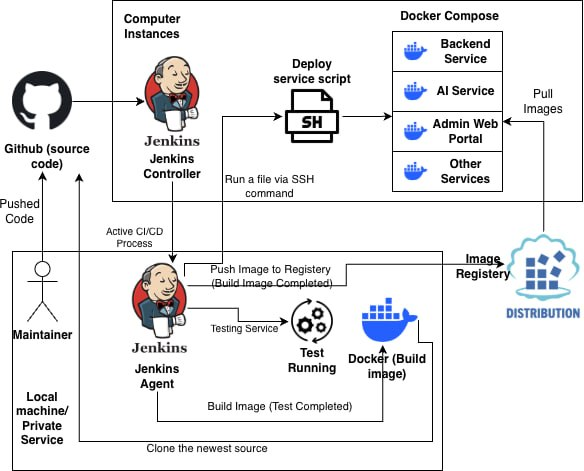
\includegraphics[width=1\textwidth]{Images/Deploy_arch.jpg}
    \vspace{10pt}
    \caption{Kiến trúc triển khai CI/CD của hệ thống}
    \label{fig:deploy_arch}
\end{figure}

\subsubsection{Giai đoạn Build và Test (Jenkins Agent)}

\textbf{Jenkins Agent} được cài đặt trên máy cục bộ (Local Machine / Private Service) của đội ngũ phát triển, chịu trách nhiệm xây dựng và kiểm tra chất lượng mã nguồn trước khi đưa lên production. Quy trình hoạt động như sau:

\begin{enumerate}
    \item \textbf{Clone mã nguồn mới nhất:} Khi Maintainer kích hoạt quy trình CI/CD, Jenkins Agent tự động clone phiên bản mã nguồn mới nhất từ GitHub repository.
    
    \item \textbf{Build Docker Image:} Agent thực hiện build Docker image cho từng service (Backend Service, AI Service, Admin Web Portal, và các service phụ trợ khác) dựa trên Dockerfile tương ứng trong mã nguồn.
    
    \item \textbf{Chạy kiểm thử (Test Running):} Sau khi build thành công, hệ thống tự động chạy bộ test (unit test, integration test) trên Docker image vừa tạo. Chỉ khi toàn bộ test suite pass, quy trình mới tiếp tục sang bước tiếp theo.
    
    \item \textbf{Đẩy Image lên Registry:} Khi test hoàn tất thành công, Jenkins Agent đẩy (push) Docker image đã được kiểm chứng lên \textbf{Image Registry} (Docker Hub hoặc private registry). Mỗi image được gắn tag version tương ứng với commit hash hoặc release version để đảm bảo khả năng truy vết và rollback.
\end{enumerate}

\subsubsection{Giai đoạn Deploy (Jenkins Controller)}

\textbf{Jenkins Controller} được cài đặt trên Compute Instance (máy chủ production), đóng vai trò điều phối việc cập nhật dịch vụ trên môi trường production:

\begin{enumerate}
    \item \textbf{Nhận thông báo từ GitHub:} Khi có mã nguồn mới được đẩy lên GitHub (pushed code), Jenkins Controller nhận webhook trigger và bắt đầu quy trình deploy.
    
    \item \textbf{Thực thi Deploy Script:} Jenkins Controller chạy deploy service script (\texttt{.sh}) thông qua lệnh SSH đến Compute Instance. Script này thực hiện:
    \begin{itemize}
        \item Kéo (pull) các Docker image mới nhất từ Image Registry.
        \item Cập nhật cấu hình Docker Compose nếu cần thiết.
        \item Khởi động lại các service bằng \texttt{docker-compose up -d} với image mới.
    \end{itemize}
    
    \item \textbf{Cập nhật dịch vụ:} Docker Compose trên server production kéo các image mới từ Registry và khởi động lại các container tương ứng, bao gồm:
    \begin{itemize}
        \item \textbf{Backend Service:} NestJS API server.
        \item \textbf{AI Service:} Cụm microservices AI (Gateway, NER, Chatbot, Recommender).
        \item \textbf{Admin Web Portal:} Trang quản trị hệ thống.
        \item \textbf{Other Services:} Các dịch vụ hỗ trợ khác (Kong Gateway, monitoring, v.v.).
    \end{itemize}
\end{enumerate}

\subsubsection{Ưu điểm của kiến trúc CI/CD}

Thiết kế CI/CD hai tầng (Agent--Controller) mang lại nhiều lợi ích:

\begin{itemize}
    \item \textbf{Tách biệt Build và Deploy:} Quá trình build nặng (compile, test) được thực hiện trên máy Agent, không ảnh hưởng đến hiệu năng server production. Server production chỉ cần pull image nhẹ và khởi động lại container.
    
    \item \textbf{Đảm bảo chất lượng:} Mọi thay đổi mã nguồn đều phải qua bước test tự động trước khi được triển khai, giảm thiểu rủi ro lỗi trên production.
    
    \item \textbf{Rollback dễ dàng:} Nhờ việc gắn tag version cho mỗi Docker image trên Registry, hệ thống có thể quay lại phiên bản trước đó nhanh chóng khi phát hiện lỗi.
    
    \item \textbf{Triển khai không gián đoạn (Zero-downtime):} Docker Compose hỗ trợ rolling update, cho phép cập nhật từng service mà không làm gián đoạn toàn bộ hệ thống.
    
    \item \textbf{Tự động hóa hoàn toàn:} Từ lúc developer push code lên GitHub đến khi service mới chạy trên production, toàn bộ quy trình được tự động hóa mà không cần can thiệp thủ công.
\end{itemize}

\subsection{Container hóa với Docker Compose}

File \texttt{docker-compose.yml} tại thư mục \texttt{dockers/} định nghĩa toàn bộ hạ tầng hệ thống, đảm bảo nhất quán giữa môi trường phát triển và production.

\subsubsection{PostgreSQL với PostGIS}

\begin{itemize}
    \item \textbf{Image:} \texttt{postgis/postgis:17-3.5} — PostgreSQL 17 tích hợp PostGIS 3.5 cho truy vấn không gian (tìm dịch vụ gần vị trí người dùng).
    \item \textbf{Khởi tạo:} Script \texttt{init-databases.sh} tự động tạo các database bổ sung cho Kong Gateway và các service phụ.
    \item \textbf{Healthcheck:} \texttt{pg\_isready} kiểm tra trạng thái sẵn sàng trước khi các service phụ thuộc khởi động.
    \item \textbf{Persistence:} Volume \texttt{pgdata} gắn vào \texttt{/var/lib/postgresql/data} giữ dữ liệu khi container restart.
\end{itemize}

\subsubsection{Redis}

\begin{itemize}
    \item \textbf{Image:} \texttt{redis:7-alpine} — phiên bản nhẹ, tối ưu cho container.
    \item \textbf{Persistence:} AOF (Append Only File) kết hợp RDB snapshot (\texttt{--save 20 1}).
    \item \textbf{Bảo mật:} Yêu cầu mật khẩu qua \texttt{--requirepass}, cấu hình từ biến môi trường.
\end{itemize}

\subsubsection{RabbitMQ Cluster (3 nodes + HAProxy)}

Hệ thống triển khai RabbitMQ dạng cluster 3 node đảm bảo tính sẵn sàng cao (High Availability):

\begin{itemize}
    \item \textbf{3 node:} \texttt{rabbitmq1} (primary), \texttt{rabbitmq2}, \texttt{rabbitmq3} tự động join cluster khi khởi động thông qua script \texttt{cluster-entrypoint.sh}.
    \item \textbf{TLS/SSL:} Certificate sinh tự động bởi container \texttt{rabbitmq-cert-gen}, mã hóa giao tiếp giữa các node và client.
    \item \textbf{HAProxy:} Container \texttt{rabbitmq-haproxy} cân bằng tải kết nối AMQP giữa 3 node, đảm bảo failover tự động.
    \item \textbf{Khởi tạo:} Container \texttt{rabbitmq-init} tạo user, vhost và phân quyền cho backend application.
\end{itemize}

\subsection{Kong API Gateway}

Kong đóng vai trò cổng vào duy nhất cho toàn bộ hệ thống, được triển khai gồm 3 thành phần Docker:

\begin{enumerate}
    \item \textbf{Kong Bootstrap (\texttt{kong-bootstrap}):} Container chạy một lần duy nhất để khởi tạo schema database cho Kong trên PostgreSQL.
    \item \textbf{Kong Control Plane (\texttt{kong-cp}):} Instance chính xử lý request. Proxy endpoint tại port 8000, Admin API tại port 8001, Manager UI tại port 8002 cho quản trị trực quan.
    \item \textbf{Kong Configurator (decK):} Sử dụng công cụ \texttt{decK} để đồng bộ cấu hình route, service, plugin từ file \texttt{kong.yml} vào Kong, đảm bảo cấu hình được version control và có thể tái tạo.
\end{enumerate}

Cấu hình route trong \texttt{kong.yml} định tuyến request đến các upstream service tương ứng (NestJS Backend, AI Gateway), đồng thời áp dụng các plugin bảo mật (rate limiting, authentication).

\subsection{Triển khai AI trên RunPod GPU Cloud}

Các mô hình AI yêu cầu GPU mạnh (đặc biệt Llama 3.1 8B với quantization 4-bit) được triển khai trên RunPod — nền tảng GPU cloud theo nhu cầu (on-demand):

\begin{itemize}
    \item \textbf{\texttt{deploy\_runpod.py}:} Script tự động hóa toàn bộ quy trình triển khai: tạo pod GPU trên RunPod, cài đặt môi trường Python và dependencies, tải mô hình từ HuggingFace, và khởi động các AI service (RAG Chatbot, Recommender, NER, Gateway).
    \item \textbf{\texttt{teardown\_runpod.py}:} Script gỡ bỏ pod và giải phóng tài nguyên GPU khi không cần thiết, tiết kiệm chi phí vận hành.
    \item \textbf{Yêu cầu phần cứng:} GPU NVIDIA với tối thiểu 16GB VRAM cho inference Llama 3.1 8B (quantized 4-bit NF4).
\end{itemize}

\subsection{Kiến trúc triển khai tổng thể}

Kiến trúc triển khai tách biệt thành hai cụm độc lập giao tiếp qua REST API:

\begin{itemize}
    \item \textbf{Cụm Backend (Server CPU):} Docker Compose chạy PostgreSQL, Redis, RabbitMQ, Kong và NestJS Backend. Triển khai trên Compute Instance và được cập nhật tự động qua Jenkins Controller.
    \item \textbf{Cụm AI (RunPod GPU):} Các microservices Python (Gateway, NER, Chatbot, Recommender) chạy trên pod GPU cloud. Có thể scale lên/xuống theo nhu cầu thực tế.
    \item \textbf{CI/CD Pipeline:} Jenkins Agent (máy cục bộ) đảm nhận build và test, đẩy image lên Registry. Jenkins Controller (server production) kéo image và triển khai tự động khi có code mới trên GitHub.
    \item \textbf{Kết nối:} Cloudflare Tunnel đảm bảo kết nối an toàn giữa hai cụm và với client bên ngoài.
\end{itemize}

Thiết kế này cho phép scale từng phần linh hoạt: tăng GPU khi lượng truy vấn AI tăng mà không ảnh hưởng đến Backend, hoặc mở rộng Backend khi lượng booking tăng mà không tốn thêm chi phí GPU. Đồng thời, quy trình CI/CD tự động hóa hoàn toàn đảm bảo mọi thay đổi được kiểm thử kỹ lưỡng trước khi lên production, giảm thiểu rủi ro và tăng tốc chu kỳ phát triển.

\newpage
\section{Kết quả thử nghiệm \& đánh giá}
\subsection{Kiểm thử chức năng (Functional Testing)}
\subsection{Kiểm thử phi chức năng (Performance, Load, Security)}
\subsection{Đánh giá hiệu quả AI trong gợi ý dịch vụ}
\subsection{Phản hồi từ người dùng thử nghiệm}
\newpage
\chapter{Kết luận \& Hướng phát triển tiếp theo}

\section{Đánh giá kết quả đạt được so với yêu cầu đề ra}

Phần này đối chiếu trực tiếp các chức năng và yêu cầu phi chức năng đã đề ra trong Chương~2 với kết quả hiện thực hóa thực tế của đồ án.

\subsection{Đánh giá chức năng}

\renewcommand{\arraystretch}{1.4}
\begin{xltabular}{\textwidth}{|p{0.05\textwidth}|X|X|p{0.08\textwidth}|}
\caption{Đối chiếu yêu cầu chức năng và kết quả đạt được} \label{tab:ketqua_chucnang} \\
\hline
\textbf{STT} & \textbf{Yêu cầu chức năng đề ra} & \textbf{Kết quả đạt được} & \textbf{Mức độ} \\
\hline
\endfirsthead
\multicolumn{4}{l}{\small\textit{(tiếp theo Bảng~\ref*{tab:ketqua_chucnang})}} \\[2pt]
\hline
\textbf{STT} & \textbf{Yêu cầu chức năng đề ra} & \textbf{Kết quả đạt được} & \textbf{Mức độ} \\
\hline
\endhead
\hline
\endfoot
\multicolumn{4}{|l|}{\textit{User App}} \\
\hline
1 & Onboarding \& Cá nhân hóa hồ sơ: đăng ký, khảo sát sở thích, khởi tạo hồ sơ tức thì & Hoàn thiện đầy đủ: đăng ký username/password, khảo sát nhu cầu sức khỏe, gợi ý dịch vụ ngay sau onboarding & Đầy đủ \\
\hline
2 & Chatbot AI tư vấn \& gợi ý dịch vụ qua hội thoại tự nhiên & Triển khai pipeline RAG (ChromaDB + Gemini), phân loại ý định, tích hợp NER để lọc theo địa điểm, hỗ trợ streaming SSE & Đầy đủ \\
\hline
3 & Tìm kiếm \& lọc nâng cao theo từ khóa, giá, vị trí, đánh giá & Tìm kiếm full-text kết hợp NER Service, lọc đa chiều, hiển thị bản đồ Mapbox & Đầy đủ \\
\hline
4 & Đặt lịch hẹn: xem slot trống, tự động thông báo, quản lý lịch hẹn & Thực hiện qua Async Checkout Queue (RabbitMQ + Redis distributed lock), thông báo push realtime & Đầy đủ \\
\hline
5 & Thanh toán đa kênh \& hệ thống đánh giá xác thực & Tích hợp MoMo (IPN webhook) và Stripe (on-device SDK + webhook), đánh giá chỉ mở sau khi hoàn thành dịch vụ & Đầy đủ \\
\hline
6 & AI trong quản trị: dashboard phân tích, phân khúc khách hàng, thông báo cá nhân hóa & Dashboard KPI, campaign notification, phân khúc người dùng theo hành vi đặt lịch & Cơ bản \\
\hline
\multicolumn{4}{|l|}{\textit{Partner Portal}} \\
\hline
7 & Đăng ký đối tác: biểu mẫu đa bước, cổng tải tài liệu pháp lý & Form đa bước, upload tài liệu qua Cloudflare R2 (presigned URL), email xác nhận nhận hồ sơ & Đầy đủ \\
\hline
8 & Cổng thông tin chờ duyệt: theo dõi trạng thái, cập nhật hồ sơ & Hiển thị trạng thái \texttt{PENDING}/\texttt{REQUIRED\_RESUBMIT} /\texttt{APPROVED}/\texttt{REJECTED}, cho phép tái nộp hồ sơ & Đầy đủ \\
\hline
9 & Booking Dashboard: xem và xử lý lịch hẹn, calendar view & Xem danh sách lịch hẹn CONFIRMED, hoàn tất dịch vụ, đánh dấu no-show, xem báo cáo doanh thu & Đầy đủ \\
\hline
10 & Quản lý dịch vụ: tạo/chỉnh sửa, gán nhân viên, cập nhật thời gian thực & CRUD dịch vụ đầy đủ, upload ảnh presigned URL, gán nhân viên theo chuyên môn & Đầy đủ \\
\hline
11 & Quản lý nhân viên \& phân quyền: tạo hồ sơ, vai trò, tài khoản cá nhân & Tạo hồ sơ bác sĩ/spa therapist, phân quyền theo role, gửi email tài khoản tự động & Đầy đủ \\
\hline
12 & Quản lý khuyến mãi: tạo ưu đãi, điều kiện linh hoạt & Chưa hiện thực hóa đầy đủ trong phiên bản hiện tại & Một phần \\
\hline
13 & Báo cáo \& phân tích kinh doanh: dashboard KPI, thống kê, xuất dữ liệu & Dashboard doanh thu, số lịch hẹn theo kỳ; chưa có xuất Excel/CSV & Cơ bản \\
\hline
\multicolumn{4}{|l|}{\textit{Admin Dashboard}} \\
\hline
14 & Xác thực \& quản lý đối tác: xét duyệt 3 chiều, quản lý tài khoản & Duyệt/Từ chối/Yêu cầu bổ sung, ghi lịch sử xét duyệt, gửi thông báo tự động & Đầy đủ \\
\hline
15 & Quản lý đánh giá \& báo cáo vi phạm & Kiểm duyệt đánh giá cơ bản; chưa có hệ thống ticket xử lý báo cáo vi phạm & Một phần \\
\hline
16 & Quản lý tài chính toàn hệ thống: GMV, đối soát, thanh toán đối tác & Dashboard tài chính, refund flow (MoMo + Stripe), PartnerRefundCase; chưa có thanh toán hàng loạt tự động & Cơ bản \\
\hline
17 & Voucher \& Campaign Management & Campaign notification center đã có; tạo mã giảm giá toàn hệ thống chưa hoàn thiện & Một phần \\
\hline
18 & Chat thời gian thực User--Partner (WebSocket) & Triển khai đầy đủ: UserChatGateway \& PartnerChatGateway, lưu lịch sử, đánh dấu đã đọc & Đầy đủ \\
\hline
\end{xltabular}

\subsection{Đánh giá yêu cầu phi chức năng}

\renewcommand{\arraystretch}{1.4}
\begin{xltabular}{\textwidth}{|p{0.20\textwidth}|X|X|p{0.08\textwidth}|}
\caption{Đánh giá yêu cầu phi chức năng} \label{tab:ketqua_phichucnang} \\
\hline
\textbf{Tiêu chí} & \textbf{Yêu cầu đề ra} & \textbf{Kết quả đạt được} & \textbf{Mức độ} \\
\hline
\endfirsthead
\multicolumn{4}{l}{\small\textit{(tiếp theo Bảng~\ref*{tab:ketqua_phichucnang})}} \\[2pt]
\hline
\textbf{Tiêu chí} & \textbf{Yêu cầu đề ra} & \textbf{Kết quả đạt được} & \textbf{Mức độ} \\
\hline
\endhead
\hline
\endfoot
Kiểm thử & Đảm bảo độ tin cậy từng thành phần & 63 file spec, 408 test case, 0 thất bại (Jest, 09/05/2026) & Vượt mức \\
\hline
Bảo mật & JWT (access 15 phút, refresh 7 ngày), RBAC 4 vai trò, OWASP Top 10 & JWT + refresh token rotation, Guard phân quyền User/Partner/Staff/Admin, input validation (class-validator) & Đầy đủ \\
\hline
Hiệu năng Chatbot & Phản hồi $\leq 20$s, relevance $\geq 85\%$ & Streaming SSE rút ngắn cảm nhận độ trễ; pipeline RAG đạt relevance $\approx 82\%$ trên bộ đánh giá nội bộ & Cơ bản \\
\hline
Kiến trúc mở rộng & Horizontal scaling độc lập từng service & Microservices tách biệt (Core, AI Gateway, NER, RAG, Recommender); Docker Compose production-ready & Đầy đủ \\
\hline
Tích hợp bên thứ ba & Payment (MoMo, Stripe), Maps, Storage & MoMo IPN + Stripe webhook + SDK on-device; Mapbox; Cloudflare R2 presigned upload & Đầy đủ \\
\hline
Xử lý đồng thời & Race condition booking không trùng slot & Redis distributed lock + RabbitMQ + transaction DB; kiểm thử race condition 4 kịch bản & Đầy đủ \\
\hline
CI/CD \& Monitoring & Pipeline tự động, Prometheus/Grafana & Triển khai pipeline CI/CD và monitoring dashboard đầy đủ & Đầy đủ \\
\hline
Uptime 99.9\% & $\leq 43$ phút downtime/tháng & Chưa có môi trường production để đo lường chính thức & Chưa đo \\
\hline
\end{xltabular}

\section{Nhận xét chung}

Qua quá trình thực hiện, đồ án đã hoàn thành \textbf{14/18 yêu cầu chức năng ở mức đầy đủ hoặc cơ bản}. Những điểm nổi bật chính:

\begin{itemize}
    \item \textbf{Về kiến trúc:} Hệ thống theo mô hình Microservices, có message queue (RabbitMQ), cache (Redis) và storage tách biệt (Cloudflare R2). Cơ chế \textit{Async Checkout Queue} với Redis distributed lock xử lý race condition đặt lịch.

    \item \textbf{Về AI Pipeline:} Hệ thống tích hợp NER, Recommender và RAG Chatbot để xử lý truy vấn tự nhiên và gợi ý dịch vụ.

    \item \textbf{Về kiểm thử:} Bộ kiểm thử đơn vị có \textbf{408 test case, 100\% pass} trên 23 module backend.

    \item \textbf{Về thanh toán:} Tích hợp MoMo và Stripe, có xử lý refund và PartnerRefundCase.
\end{itemize}

Các chức năng còn ở mức \textit{một phần} chủ yếu là nhóm marketing và vận hành nâng cao, không ảnh hưởng luồng nghiệp vụ cốt lõi.

\section{Hạn chế}

\begin{itemize}
    \item \textbf{CI/CD và Monitoring chưa hoàn thiện ở mức production:} Có pipeline và dashboard cơ bản nhưng chưa có cảnh báo tự động/SLO rõ ràng.

    \item \textbf{Chức năng marketing chưa hoàn chỉnh:} Khuyến mãi và voucher mới ở mức cơ bản.

    \item \textbf{Phụ thuộc bên thứ ba:} Thanh toán, bản đồ và lưu trữ phụ thuộc API bên ngoài.
\end{itemize}

\section{Hướng phát triển tiếp theo}

\begin{itemize}
    \item \textbf{Hoàn thiện phạm vi còn thiếu:} Xây dựng voucher, ticket hỗ trợ và xuất báo cáo Excel/CSV.

    \item \textbf{Nâng cấp AI Pipeline:} Mở rộng corpus y tế Việt Nam và tối ưu retrieval bằng hybrid search.

    \item \textbf{Triển khai DevOps \& Monitoring:} Hoàn thiện CI/CD, thêm Prometheus/Grafana và alerting tự động.

    \item \textbf{Tích hợp Telehealth:} Bổ sung Video Call (WebRTC) cho tư vấn từ xa.

    \item \textbf{Mở rộng hệ sinh thái IoT:} Kết nối smartwatch để thu thập chỉ số sức khỏe tự động.
\end{itemize}
\newpage
%%%%%%%%%%%%%%%%%OUTRO%%%%%%%%%%%%%%%%%%%
\addcontentsline{toc}{chapter}{Tài Liệu Tham Khảo}
\renewcommand{\bibname}{Tài liệu tham khảo}

\begin{thebibliography}{99}
% --- Nhóm Công nghệ ---
\bibitem{flutter}
Google, ``Tài liệu Flutter,'' \textit{flutter.dev}. [Trực tuyến]. Truy cập: https://flutter.dev/docs. [Truy cập: 10/2025].

\bibitem{nestjs}
NestJS, ``Tài liệu NestJS,'' \textit{docs.nestjs.com}. [Trực tuyến]. Truy cập: https://docs.nestjs.com/. [Truy cập: 10/2025].

\bibitem{nextjs}
Vercel, ``Tài liệu Next.js,'' \textit{nextjs.org}. [Trực tuyến]. Truy cập: https://nextjs.org/docs. [Truy cập: 10/2025].

% --- Nhóm Kiến trúc ---
\bibitem{microservices}
M. Fowler, ``Kiến trúc Microservices,'' \textit{martinfowler.com}, 2014. [Trực tuyến]. Truy cập: https://martinfowler.com/articles/microservices.html. [Truy cập: 10/2025].

\bibitem{postgres}
Nhóm Phát triển Toàn cầu PostgreSQL, ``Tài liệu PostgreSQL 15,'' \textit{postgresql.org}. [Trực tuyến]. Truy cập: https://www.postgresql.org/docs/15/. [Truy cập: 10/2025].

% --- Nhóm AI/NLP ---
\bibitem{rag}
P. Lewis \textit{và cộng sự}, ``Sinh văn bản tăng cường truy xuất cho các tác vụ NLP chuyên sâu về tri thức,'' trong \textit{Kỷ yếu Hội nghị Hệ thống Xử lý Thông tin Neural (NeurIPS)}, 2020.

\bibitem{lora}
E. J. Hu \textit{và cộng sự}, ``LoRA: Điều chỉnh thứ hạng thấp của các mô hình ngôn ngữ lớn,'' \textit{arXiv preprint arXiv:2106.09685}, 2021.

\bibitem{langchain}
LangChain, ``Tài liệu LangChain,'' \textit{python.langchain.com}. [Trực tuyến]. Truy cập: http://python.langchain.com. [Truy cập: 10/2025].

\bibitem{peft}
Hugging Face, ``PEFT: Phương pháp tinh chỉnh hiệu quả tham số tiên tiến,'' \textit{huggingface.co}. [Trực tuyến]. Truy cập: https://huggingface.co/docs/peft. [Truy cập: 10/2025].

% --- Nhóm Hệ thống tham khảo ---
\bibitem{bookingcare}
BookingCare, ``Nền tảng y tế sức khỏe toàn diện,'' \textit{bookingcare.vn}. [Trực tuyến]. Truy cập: https://bookingcare.vn/. [Truy cập: 10/2025].

\bibitem{jiohealth}
Jio Health, ``Trang chủ Jio Health,'' \textit{jiohealth.com}. [Trực tuyến]. Truy cập: https://jiohealth.com/. [Truy cập: 10/2025].

\end{thebibliography}
\newpage
\appendix
\chapter{Chi tiết Mockup UI/UX}
\label{appendix:mockup_ui}

Phụ lục này trình bày chi tiết thiết kế giao diện cho các nhóm chức năng bổ sung của ứng dụng di động Healytics, bổ sung cho phần thiết kế đã được trình bày tại Chương 5.

\subsection{Survey - Khảo sát người dùng}
\begin{figure}[H]
    \centering
    
    % --- Hàng 1 ---
    \begin{subfigure}[b]{0.24\textwidth}
        \centering
        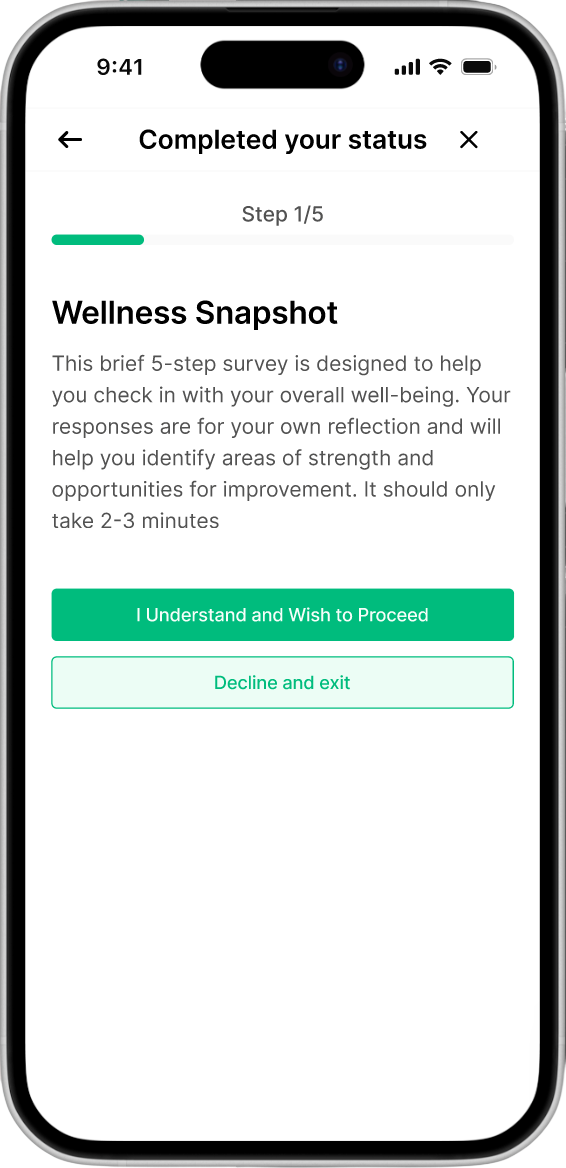
\includegraphics[width=\linewidth]{Images/uiux/survey/survey_step1.png}
        \caption{Survey Step 1}
    \end{subfigure}
    \hfill
    \begin{subfigure}[b]{0.24\textwidth}
        \centering
        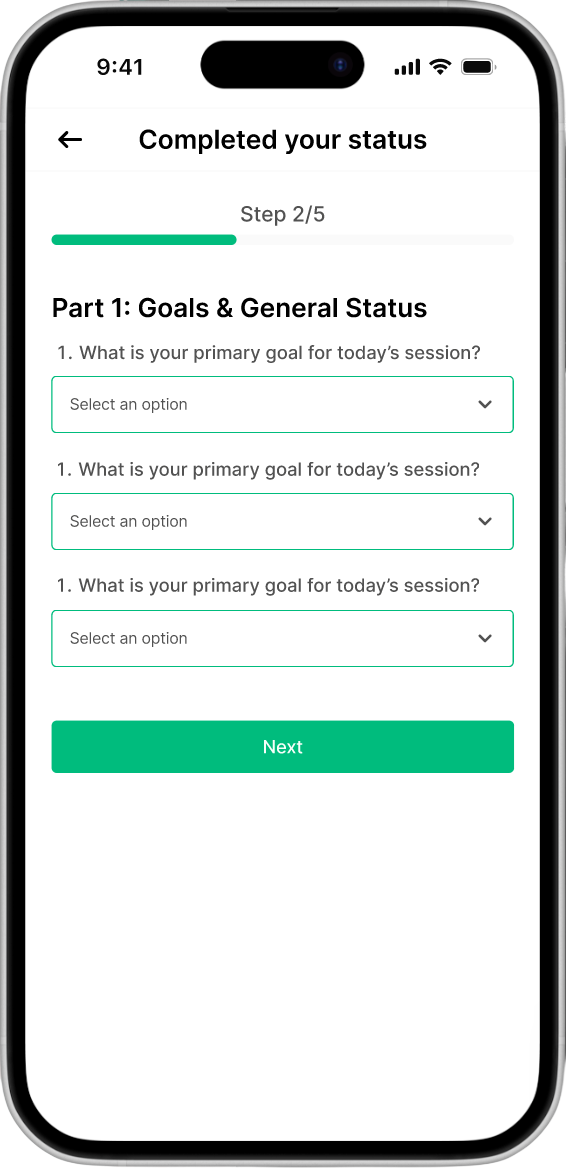
\includegraphics[width=\linewidth]{Images/uiux/survey/survey_step2.png}
        \caption{Survey Step 2}
    \end{subfigure}
    \hfill
    \begin{subfigure}[b]{0.24\textwidth}
        \centering
        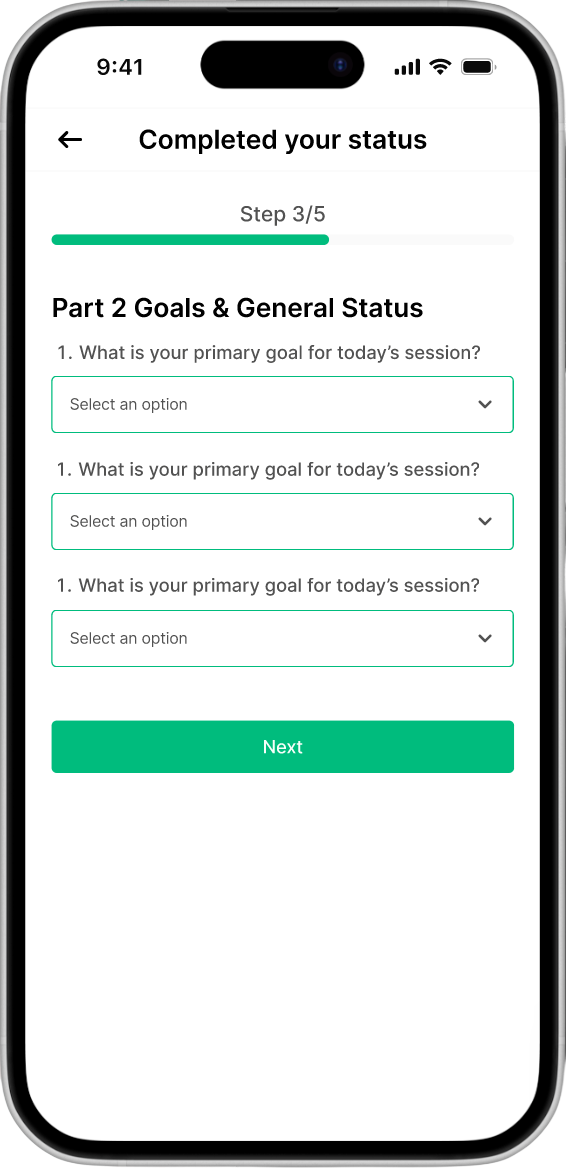
\includegraphics[width=\linewidth]{Images/uiux/survey/survey_step3.png}
        \caption{Survey Step 3}
    \end{subfigure}
    \hfill
    \begin{subfigure}[b]{0.24\textwidth}
        \centering
        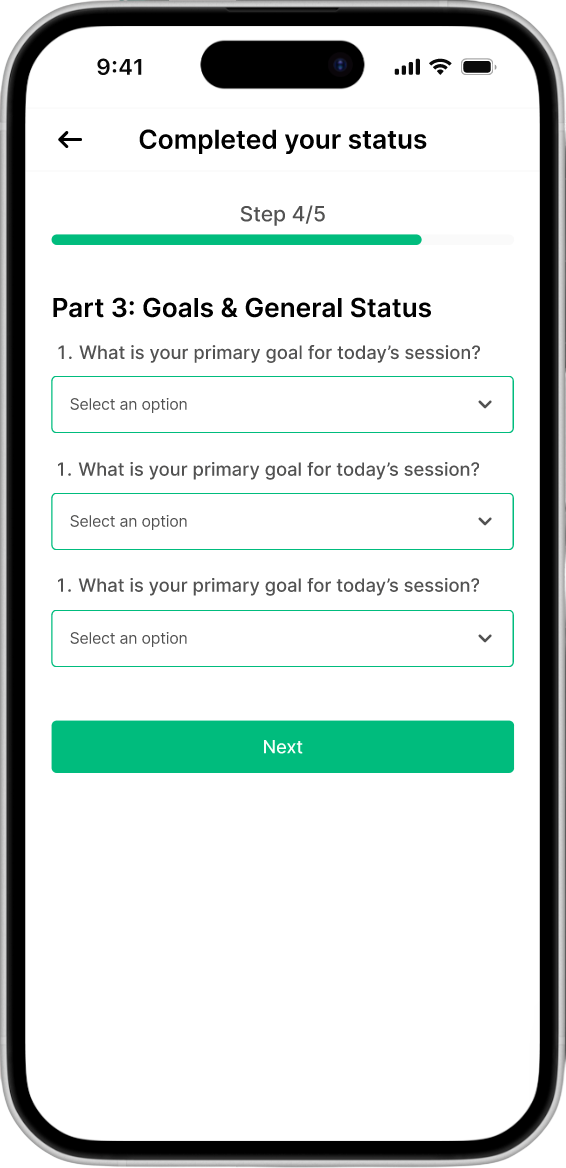
\includegraphics[width=\linewidth]{Images/uiux/survey/survey_step4.png}
        \caption{Survey Step 4}
    \end{subfigure}
    
    \vspace{1em}
    
    % --- Hàng 2 ---
    \begin{subfigure}[b]{0.24\textwidth}
        \centering
        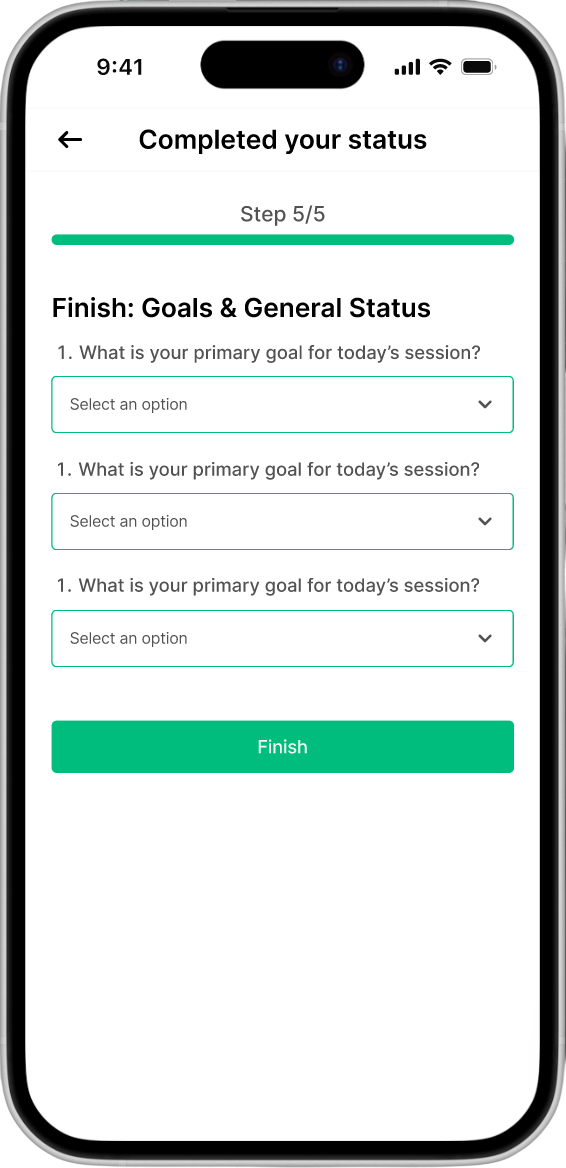
\includegraphics[width=\linewidth]{Images/uiux/survey/survey_step5.png}
        \caption{Survey Step 5}
    \end{subfigure}
    \hfill
    \begin{subfigure}[b]{0.24\textwidth}
    \end{subfigure}
    \hfill
    \begin{subfigure}[b]{0.24\textwidth}
    \end{subfigure}
    \hfill
    \begin{subfigure}[b]{0.24\textwidth}
    \end{subfigure}
    
    \vspace{1em}
    \caption{Giao diện Survey}
\end{figure}

\subsection{Provider Service - Chi tiết dịch vụ}
\begin{figure}[H]
    \centering
    
    % --- Hàng 1 ---
    \begin{subfigure}[b]{0.24\textwidth}
        \centering
        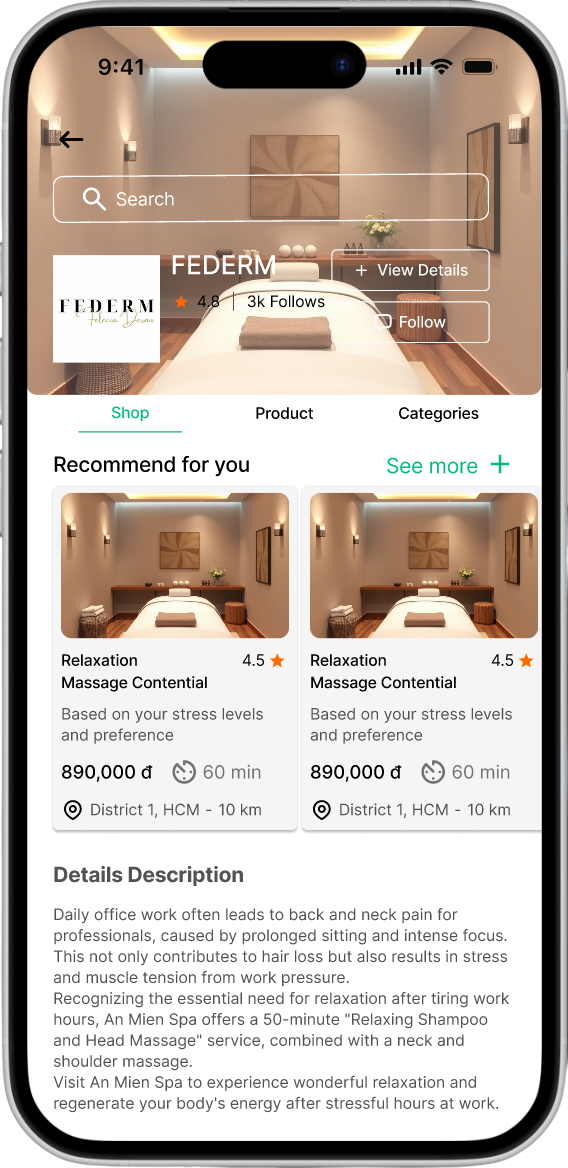
\includegraphics[width=\linewidth]{Images/uiux/provider_service/provider_details.png}
        \caption{Provider Details}
    \end{subfigure}
    \hfill
    \begin{subfigure}[b]{0.24\textwidth}
        \centering
        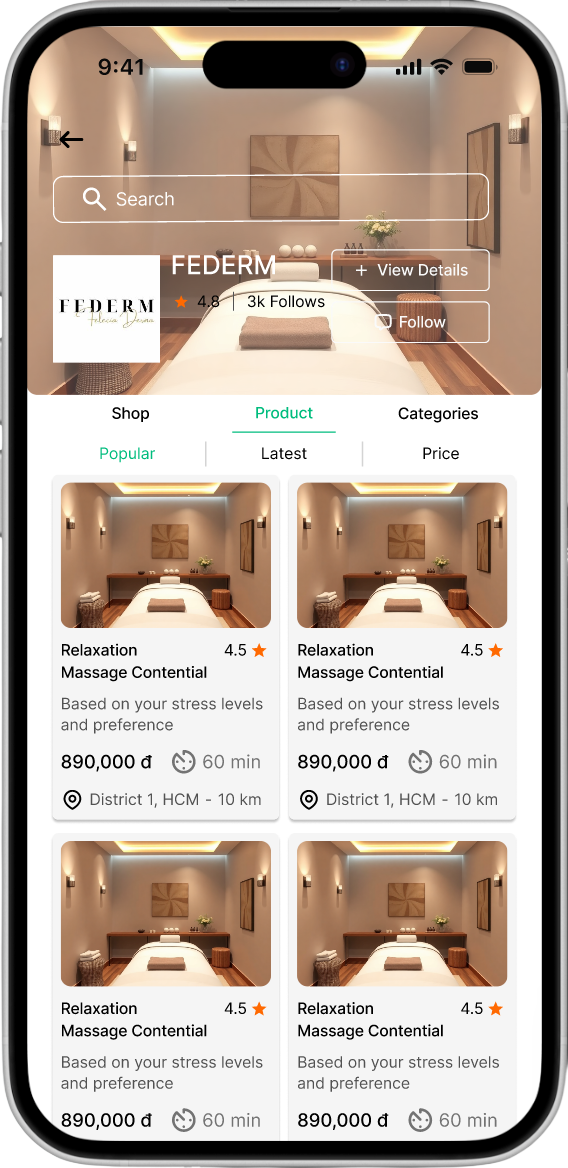
\includegraphics[width=\linewidth]{Images/uiux/provider_service/provider_details_2.png}
        \caption{Provider Details 2}
    \end{subfigure}
    \hfill
    \begin{subfigure}[b]{0.24\textwidth}
        \centering
        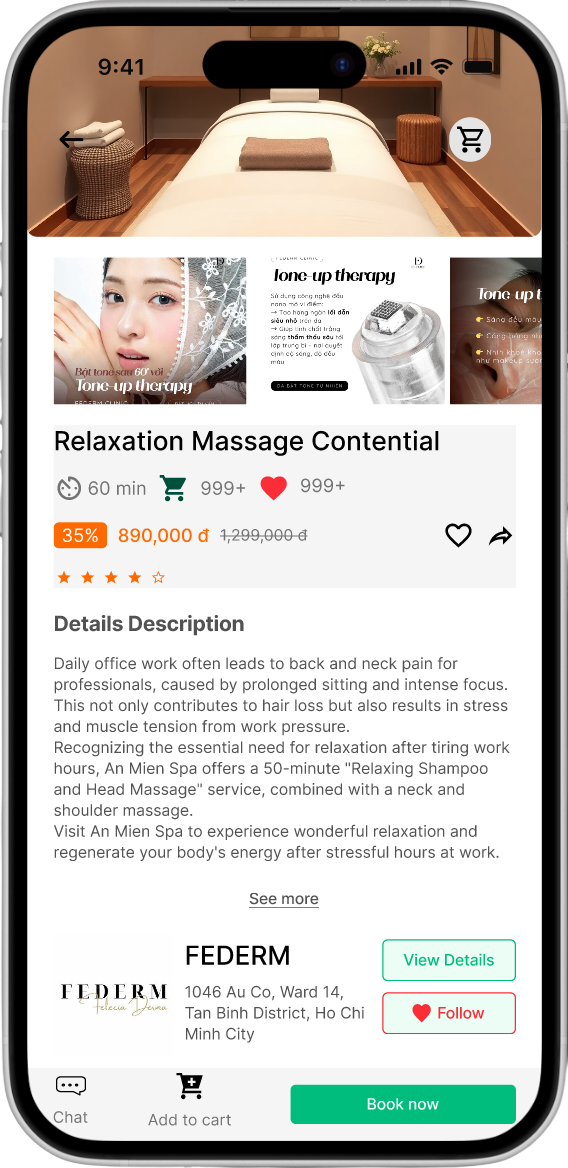
\includegraphics[width=\linewidth]{Images/uiux/provider_service/service_details_1.png}
        \caption{Service Details 1}
    \end{subfigure}
    \hfill
    \begin{subfigure}[b]{0.24\textwidth}
        \centering
        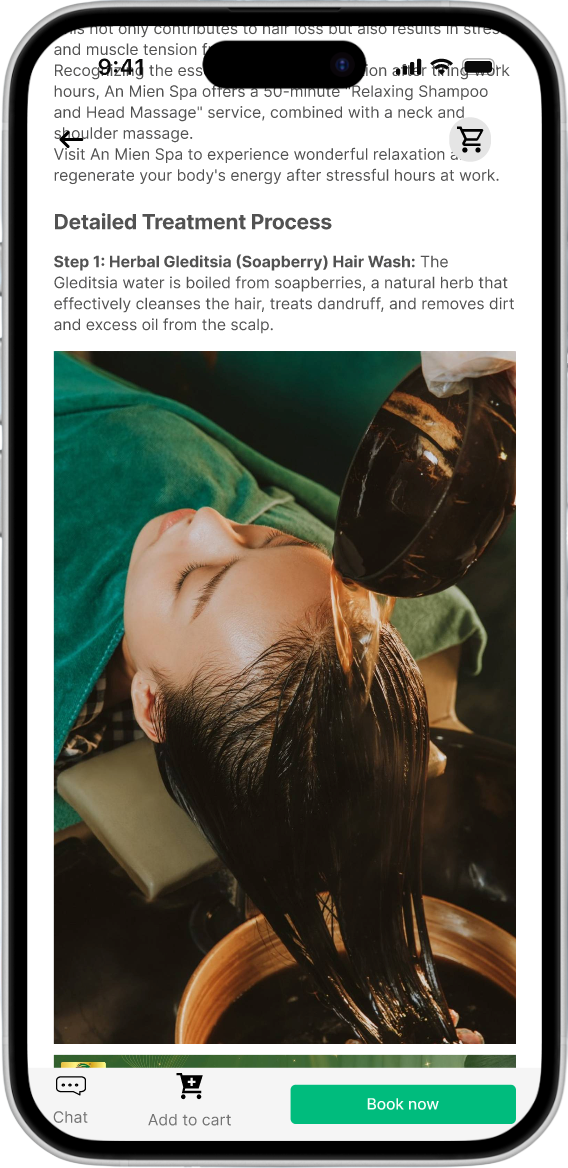
\includegraphics[width=\linewidth]{Images/uiux/provider_service/service_details_2.png}
        \caption{Service Details 2}
    \end{subfigure}
    
    \vspace{1em}
    
    % --- Hàng 2 ---
    \begin{subfigure}[b]{0.24\textwidth}
        \centering
        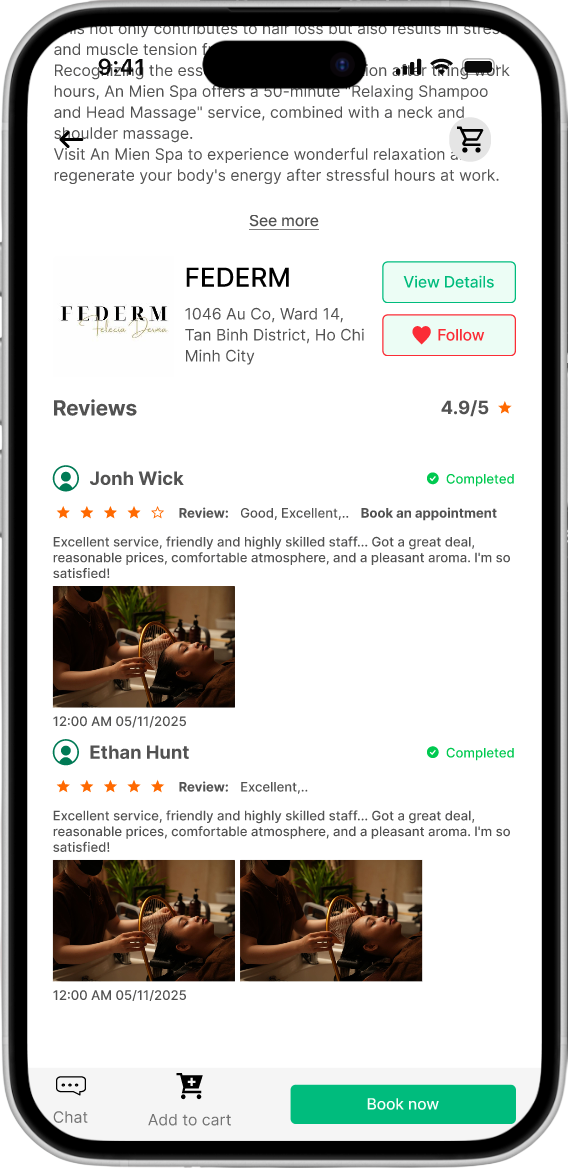
\includegraphics[width=\linewidth]{Images/uiux/provider_service/service_details_3.png}
        \caption{Service Details 3}
    \end{subfigure}
    \hfill
    \begin{subfigure}[b]{0.24\textwidth}
    \end{subfigure}
    \hfill
    \begin{subfigure}[b]{0.24\textwidth}
    \end{subfigure}
    \hfill
    \begin{subfigure}[b]{0.24\textwidth}
    \end{subfigure}
    
    \vspace{1em}
    \caption{Giao diện Provider Service}
\end{figure}

\subsection{Checkout - Thanh toán}
\begin{figure}[H]
    \centering
    
    % --- Hàng 1 ---
    \begin{subfigure}[b]{0.24\textwidth}
        \centering
        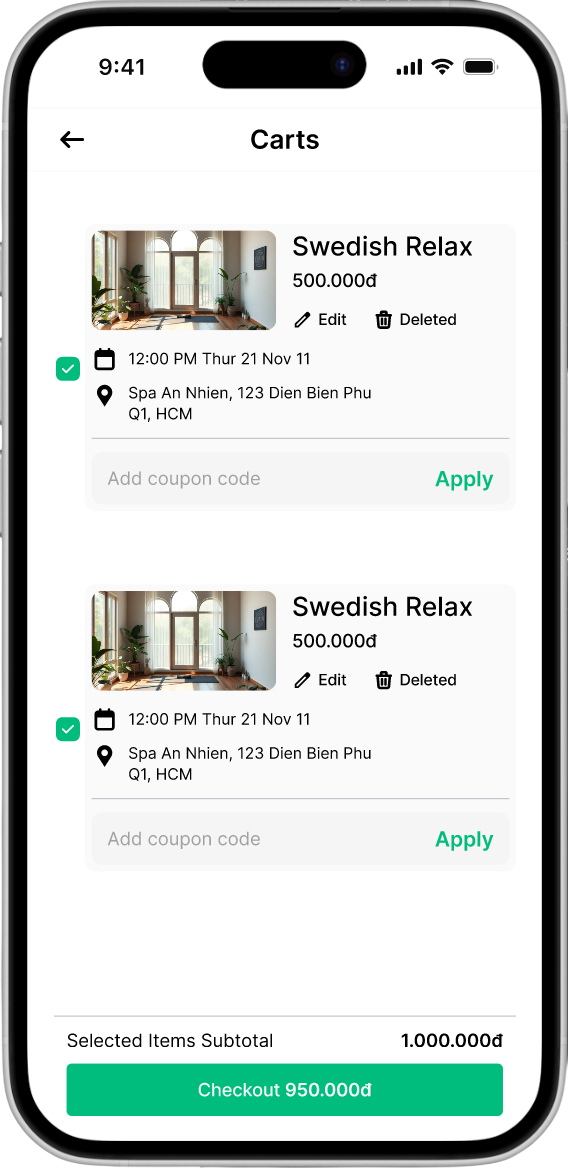
\includegraphics[width=\linewidth]{Images/uiux/checkout/carr_manager.png}
        \caption{Cart Manager}
    \end{subfigure}
    \hfill
    \begin{subfigure}[b]{0.24\textwidth}
        \centering
        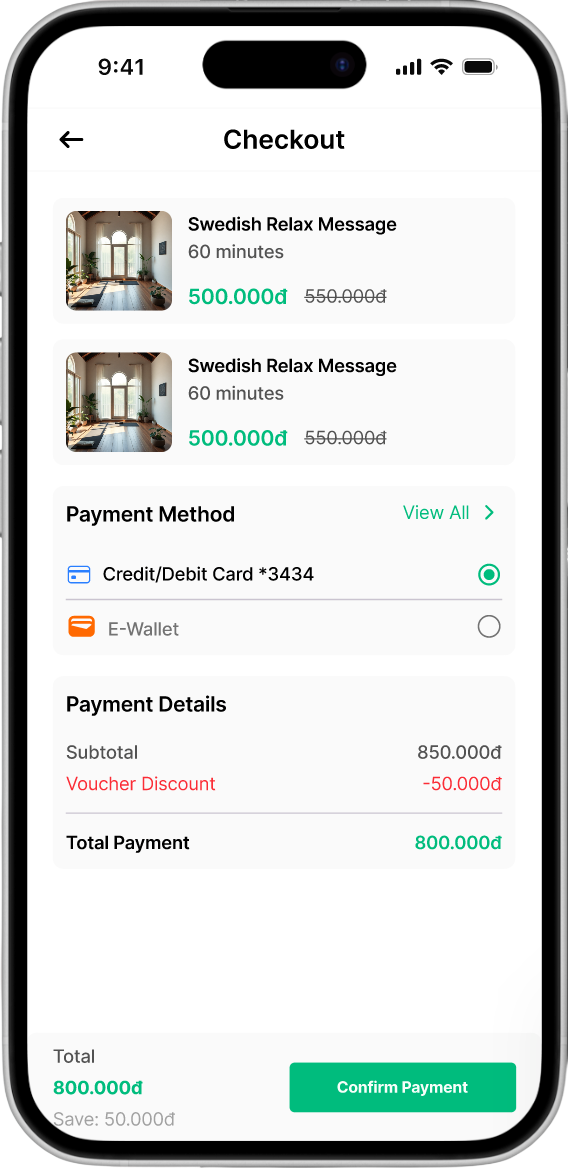
\includegraphics[width=\linewidth]{Images/uiux/checkout/checkout.png}
        \caption{Checkout}
    \end{subfigure}
    \hfill
    \begin{subfigure}[b]{0.24\textwidth}
        \centering
        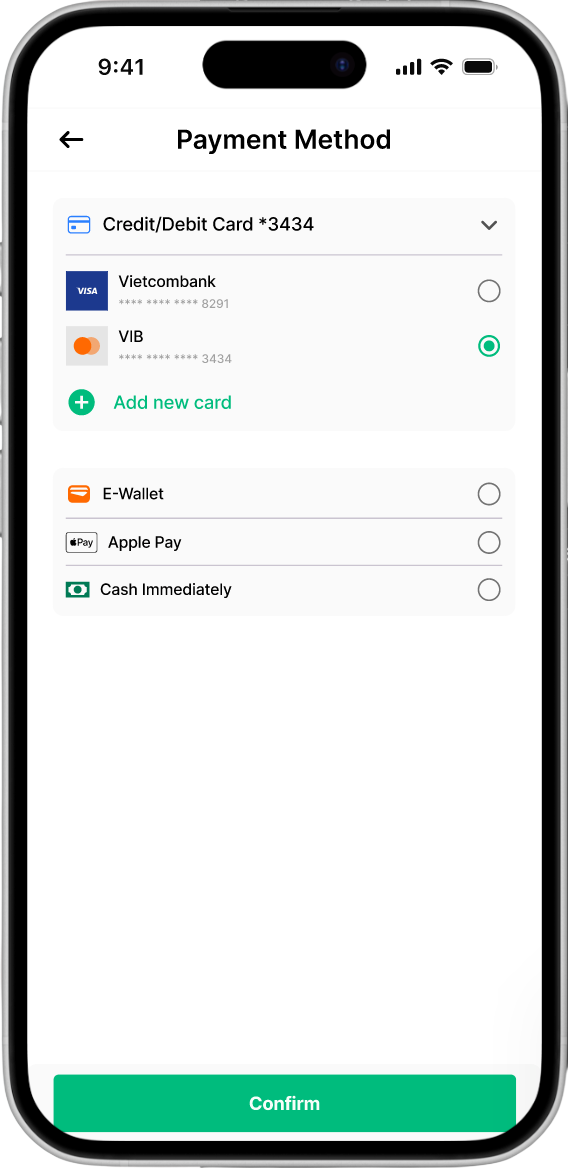
\includegraphics[width=\linewidth]{Images/uiux/checkout/select_payment_method.png}
        \caption{Select Payment Method}
    \end{subfigure}
    \hfill
    \begin{subfigure}[b]{0.24\textwidth}
    \end{subfigure}
    
    \vspace{1em}
    \caption{Giao diện Checkout}
\end{figure}

\chapter{Phụ lục kết quả đánh giá Recommender}
\label{appendix:recommender_eval}

Phụ lục này tổng hợp đầy đủ các hình trực quan từ hai baseline \texttt{chatbot\_baseline\_v1} và \texttt{home\_baseline\_v1} trong thí nghiệm đánh giá hệ thống gợi ý dịch vụ.

\begin{figure}[H]
    \centering
    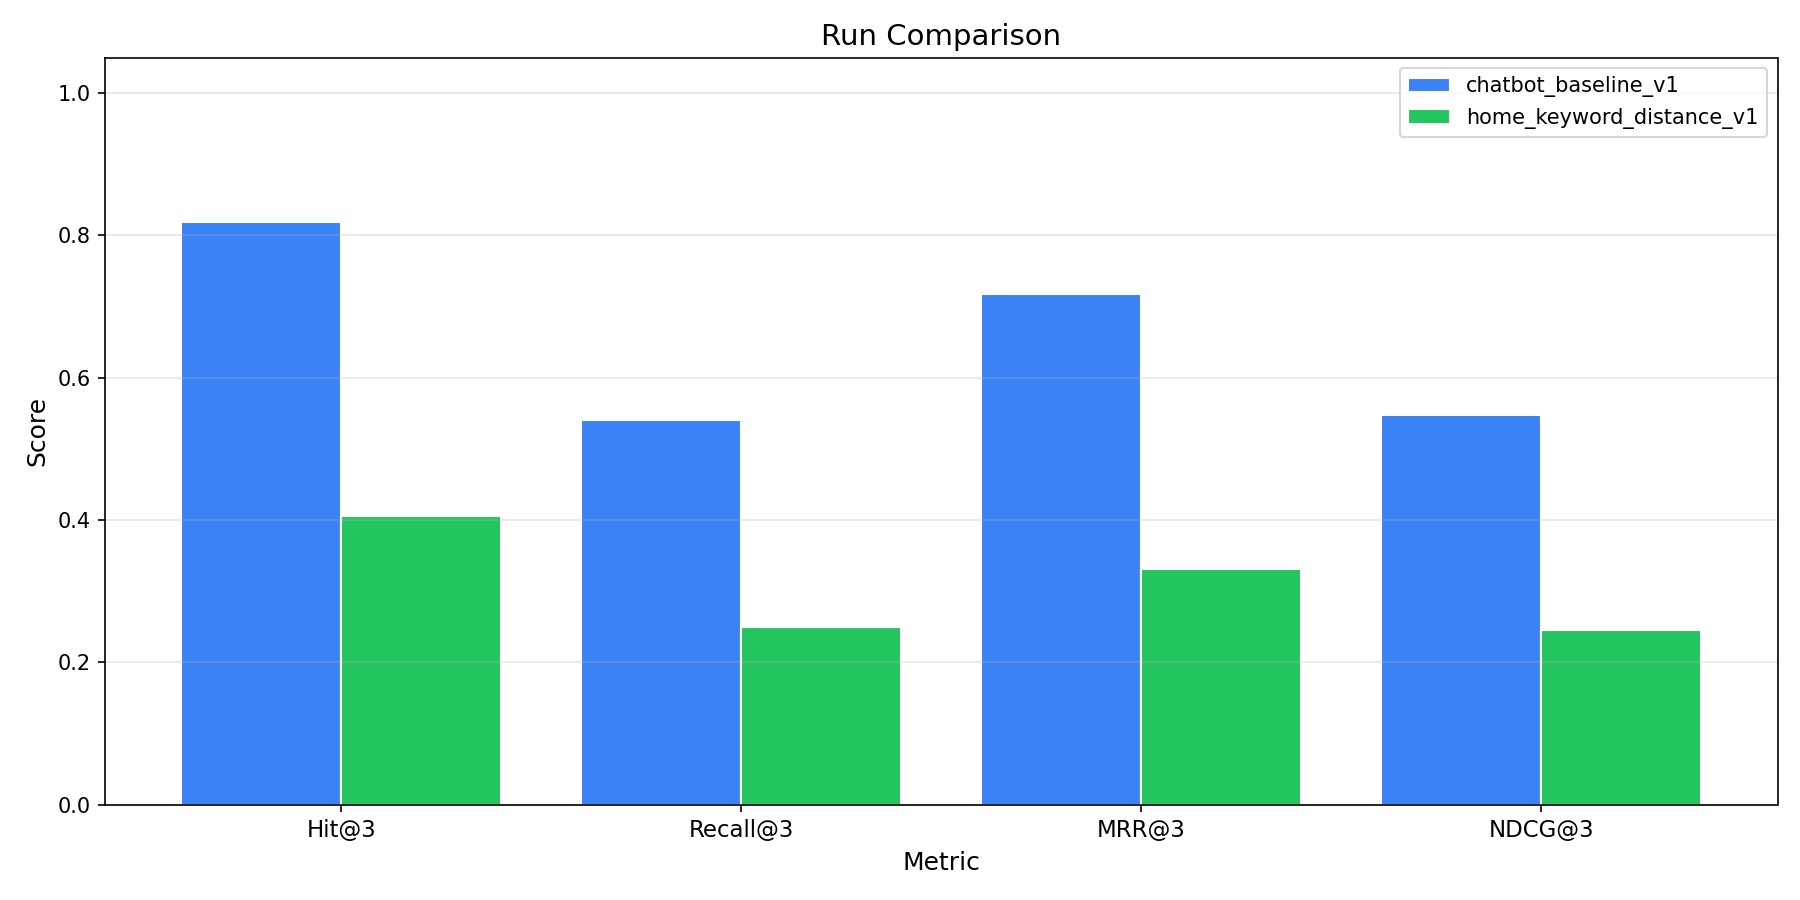
\includegraphics[width=0.92\textwidth]{Images/evaluation/recommender/run_comparison.png}
    \caption{Biểu đồ so sánh hai baseline \texttt{chatbot\_baseline\_v1} và \texttt{home\_baseline\_v1} theo Hit@3, Recall@3, MRR@3, NDCG@3}
    \label{fig:appendix_rec_run_compare}
\end{figure}

\subsection{Baseline Chatbot: phân rã theo chủ đề và nhiễu}

\begin{figure}[H]
    \centering
    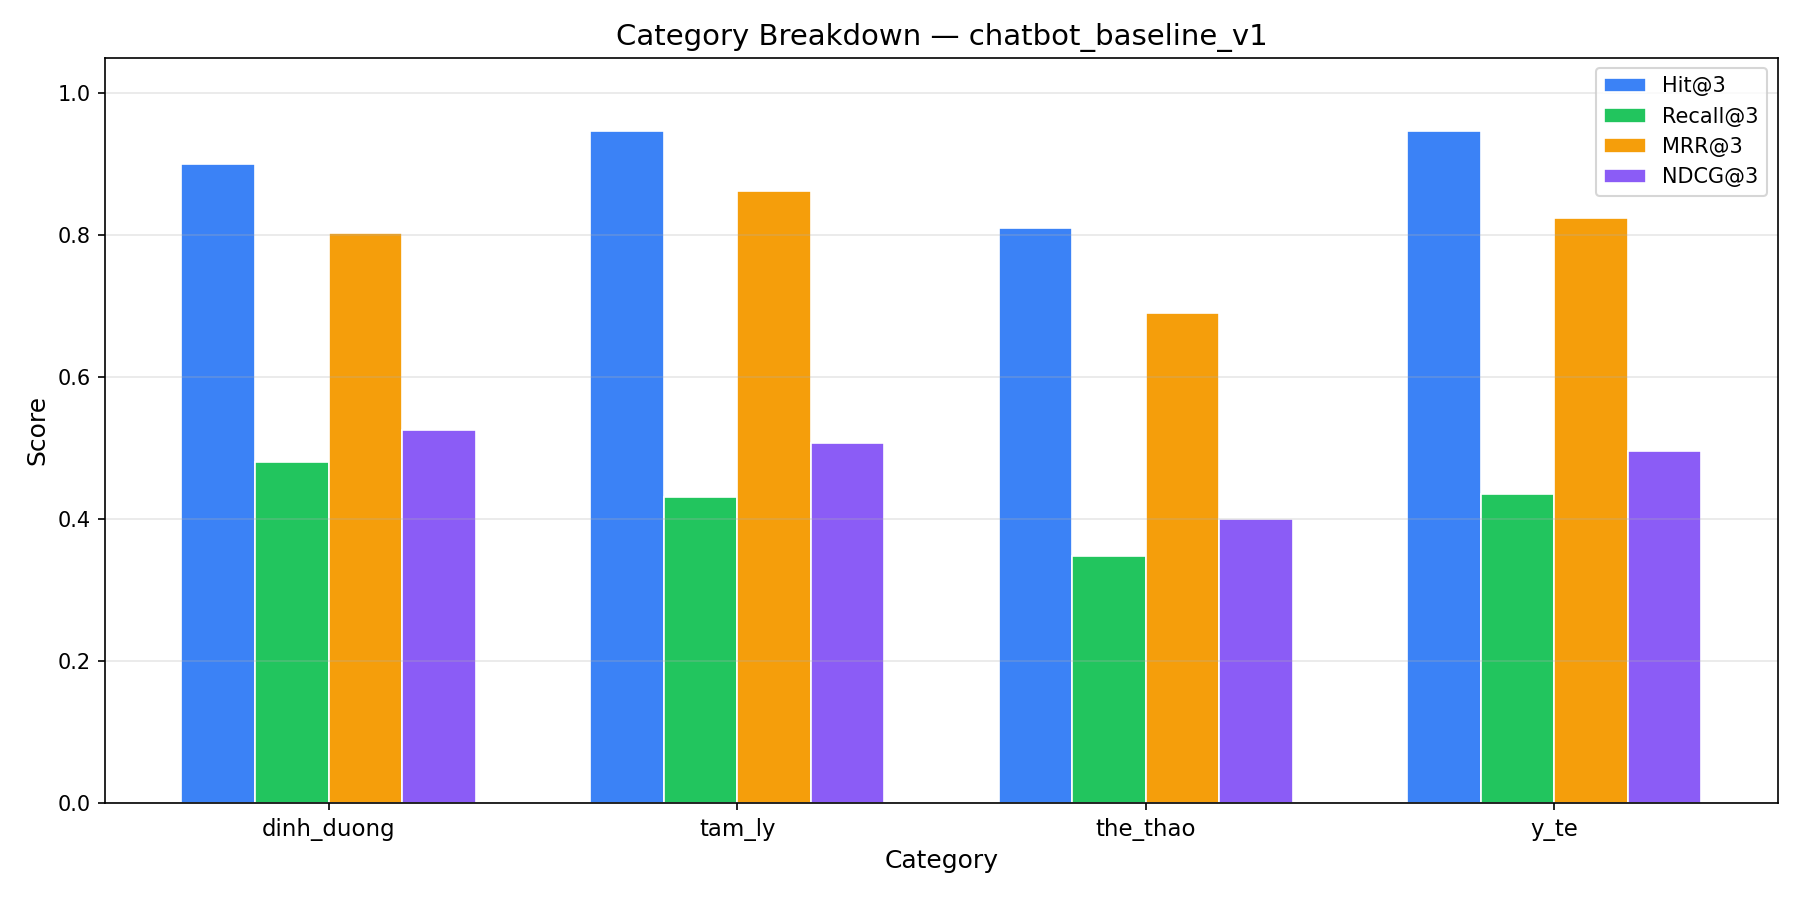
\includegraphics[width=0.92\textwidth]{Images/evaluation/recommender/category_breakdown_chatbot_baseline_v1.png}
    \caption{Phân rã chất lượng theo nhóm chủ đề của \texttt{chatbot\_baseline\_v1}}
    \label{fig:appendix_chatbot_category_breakdown}
\end{figure}

\begin{figure}[H]
    \centering
    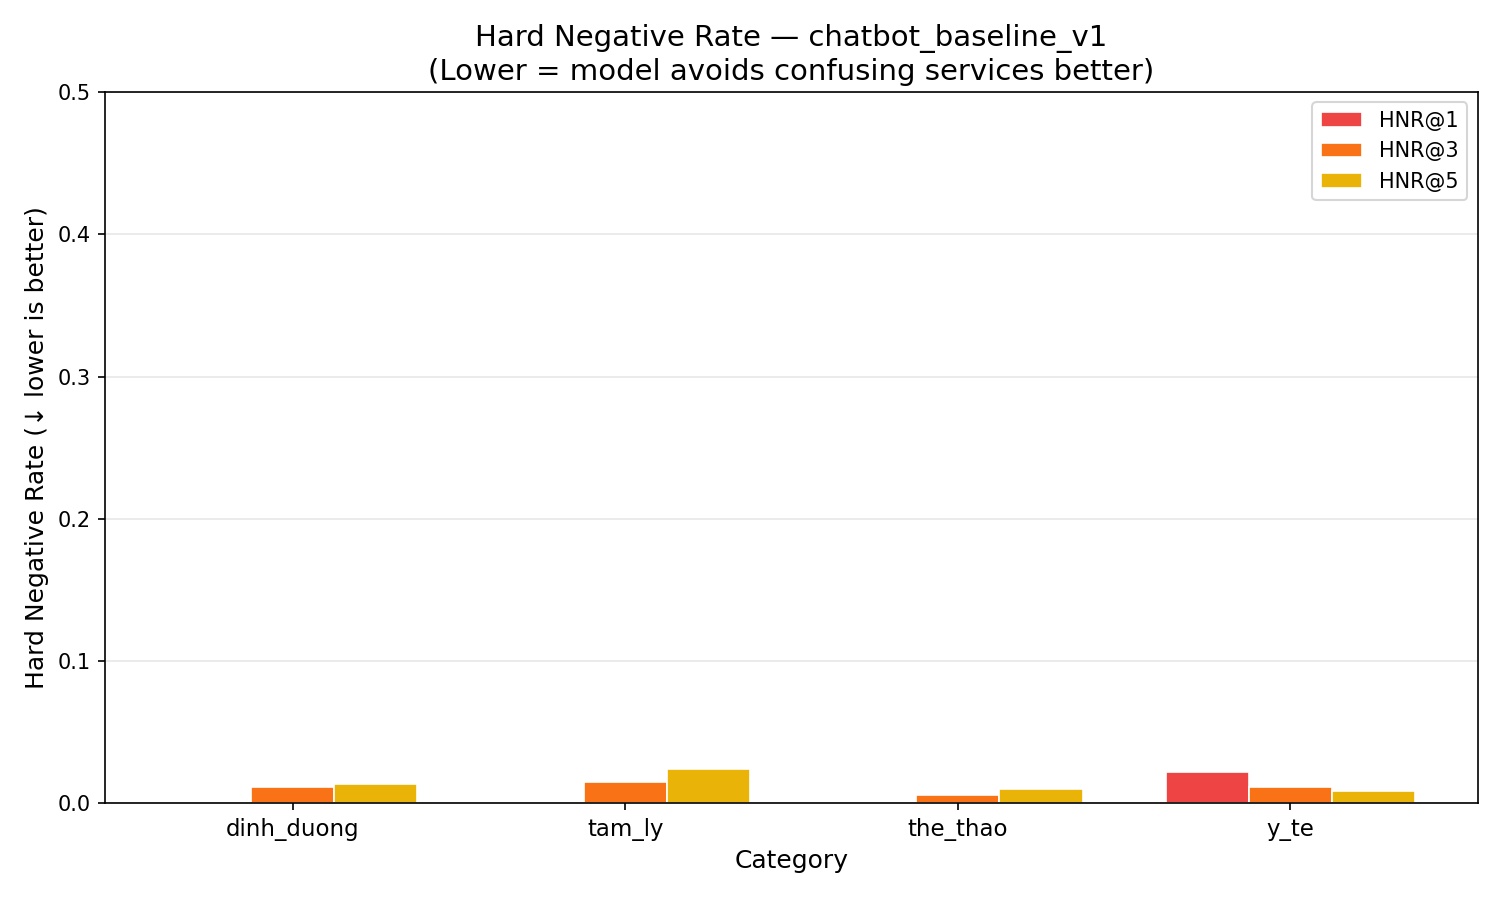
\includegraphics[width=0.92\textwidth]{Images/evaluation/recommender/hnr_breakdown_chatbot_baseline_v1.png}
    \caption{Hard Negative Rate theo chủ đề của \texttt{chatbot\_baseline\_v1}}
    \label{fig:appendix_chatbot_hnr_breakdown}
\end{figure}

\subsection{Phân bố score retrieval}

\begin{figure}[H]
    \centering
    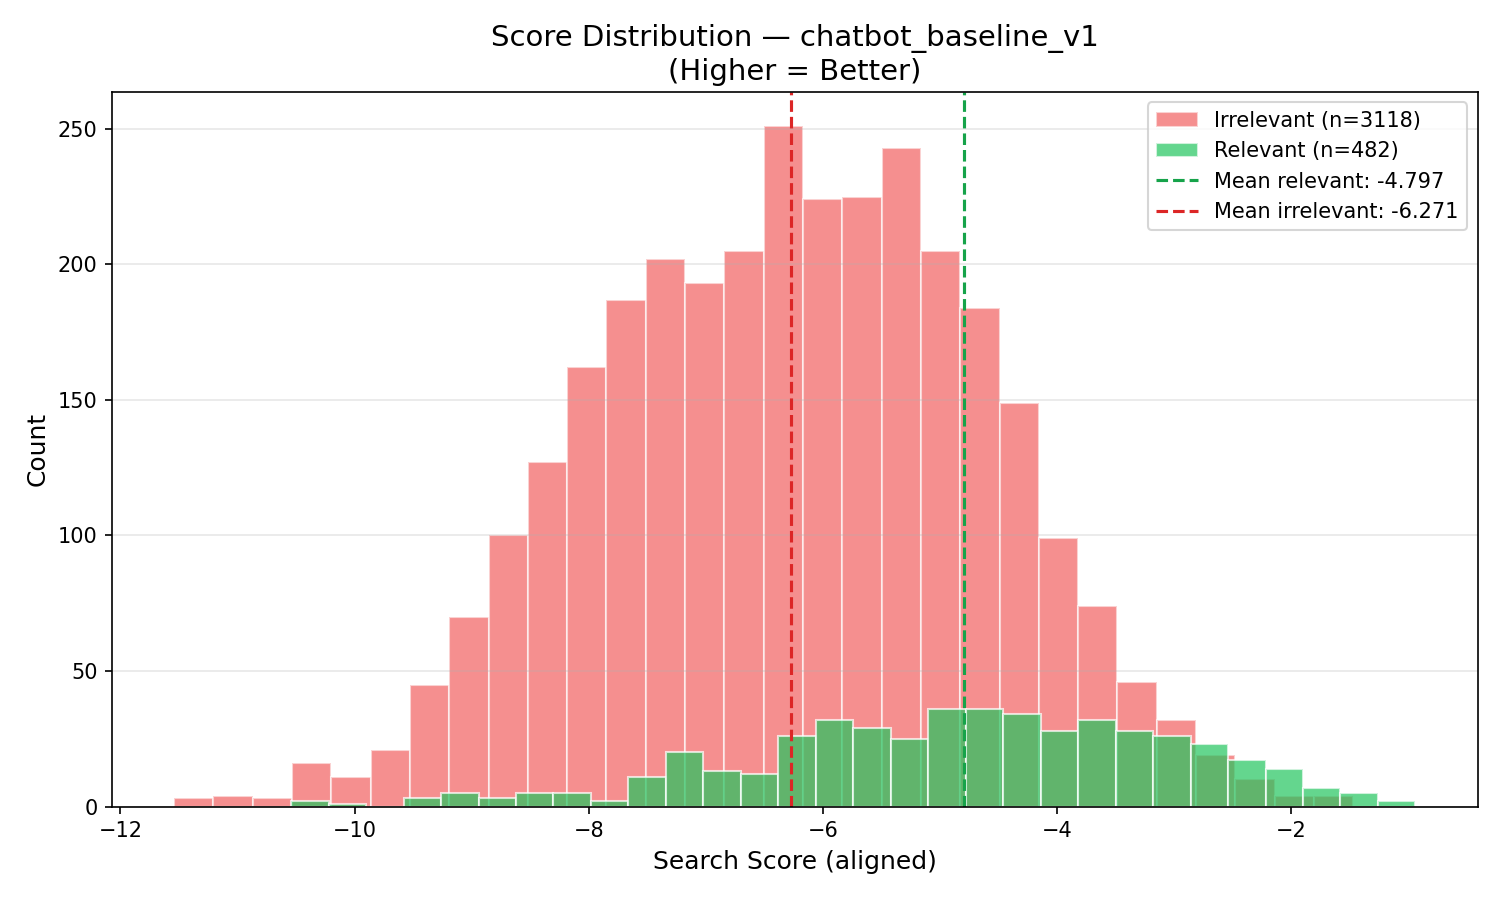
\includegraphics[width=0.92\textwidth]{Images/evaluation/recommender/cosine_dist_chatbot_chatbot_baseline_v1.png}
    \caption{Phân bố score retrieval của \texttt{chatbot\_baseline\_v1}}
    \label{fig:appendix_chatbot_score_dist}
\end{figure}

\begin{figure}[H]
    \centering
    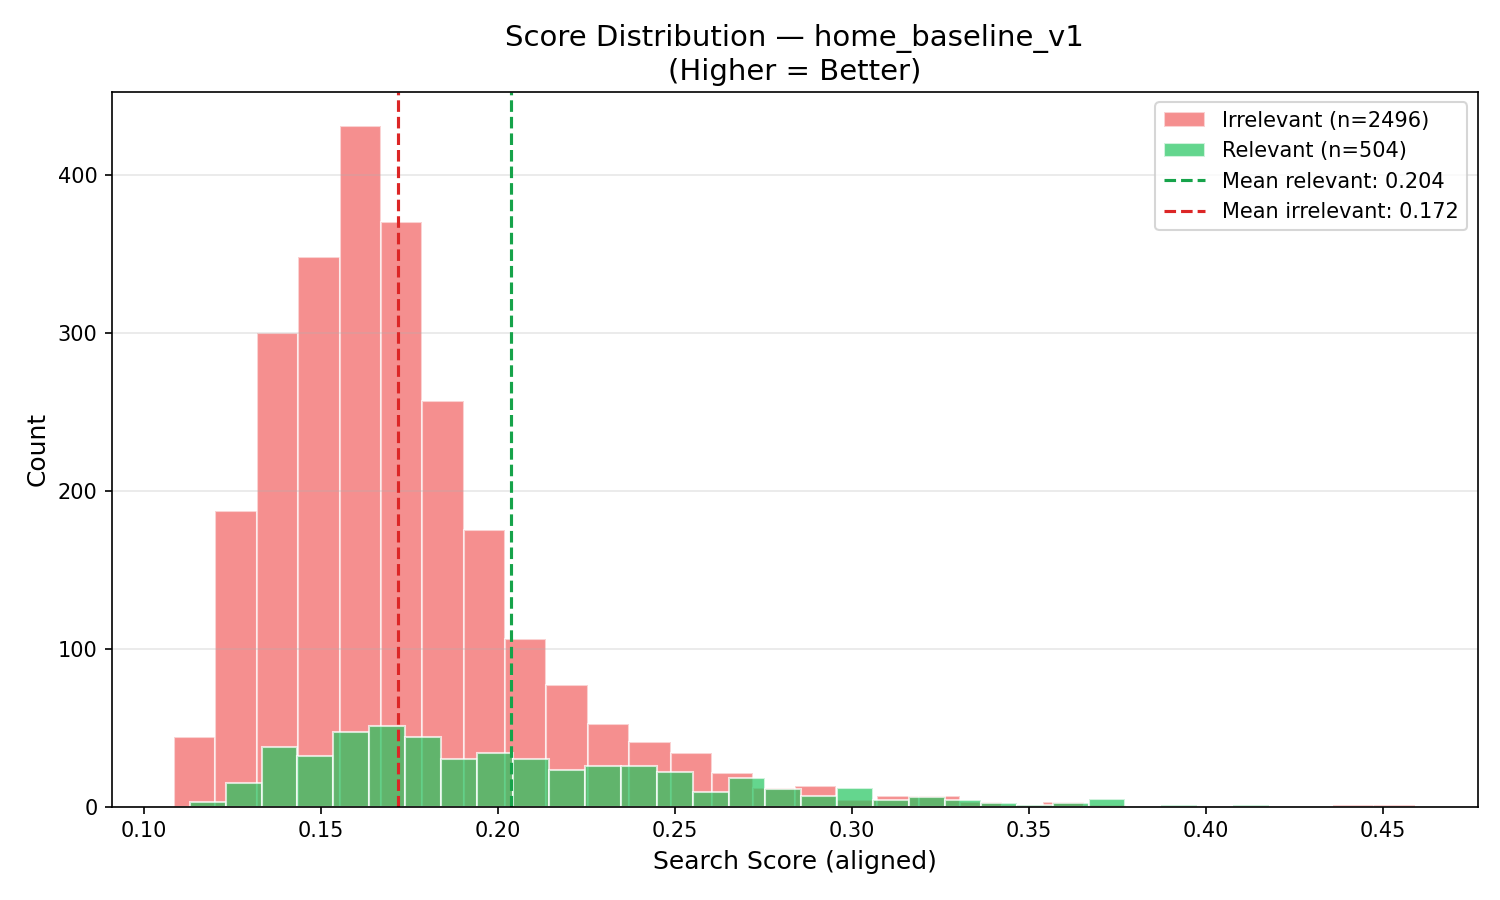
\includegraphics[width=0.92\textwidth]{Images/evaluation/recommender/cosine_dist_home_home_baseline_v1.png}
    \caption{Phân bố score retrieval của \texttt{home\_baseline\_v1}}
    \label{fig:appendix_home_score_dist}
\end{figure}

\subsection{Phân bố độ trễ}

\begin{figure}[H]
    \centering
    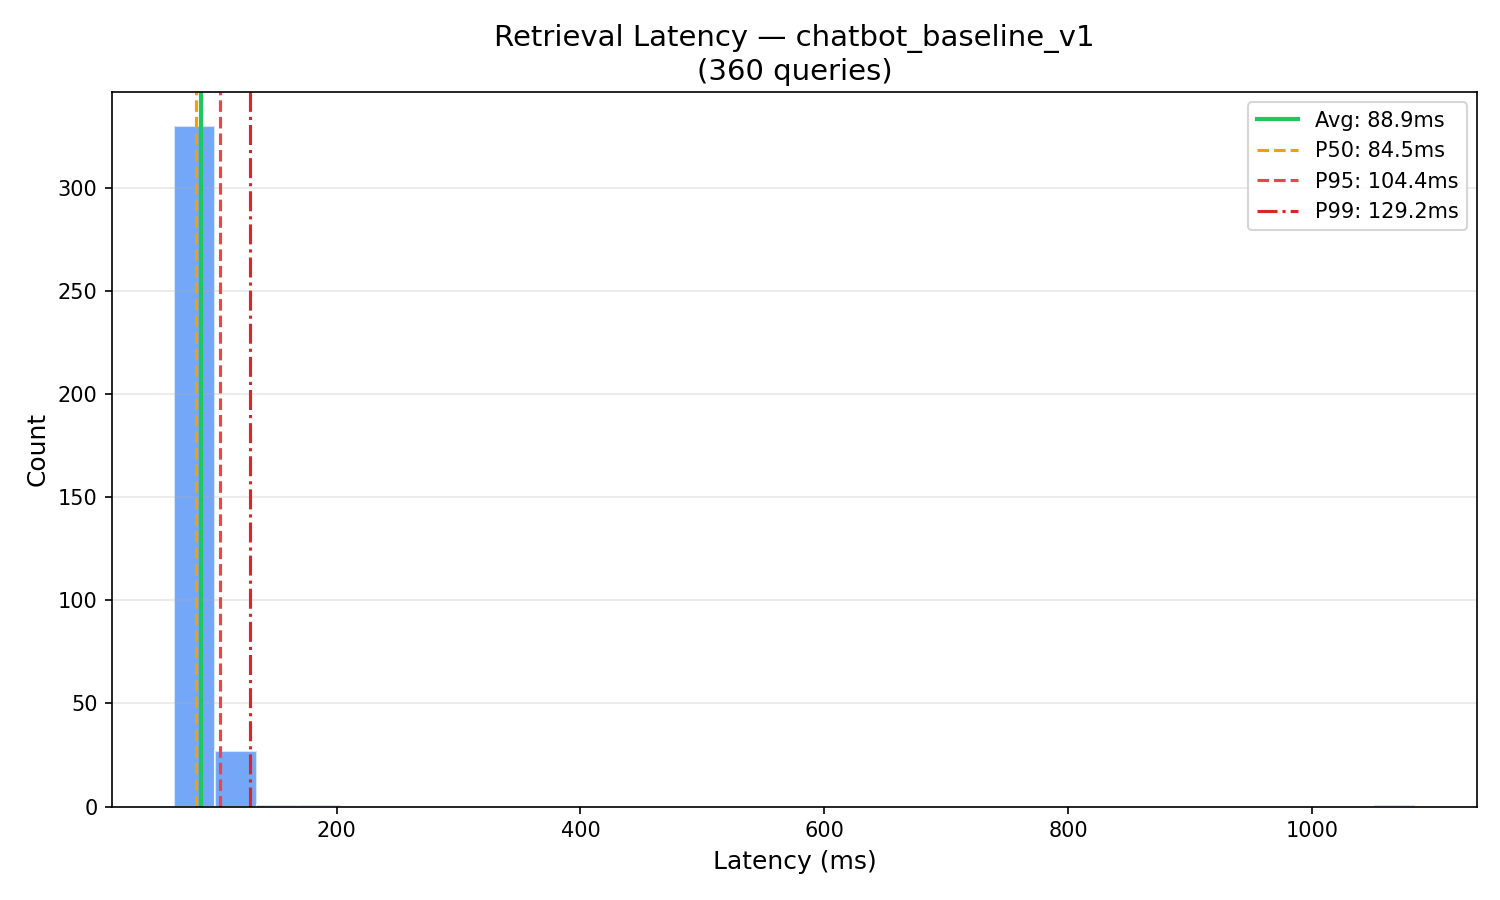
\includegraphics[width=0.92\textwidth]{Images/evaluation/recommender/latency_dist_chatbot_baseline_v1.png}
    \caption{Phân bố độ trễ truy xuất của \texttt{chatbot\_baseline\_v1}}
    \label{fig:appendix_chatbot_latency_dist}
\end{figure}

\begin{figure}[H]
    \centering
    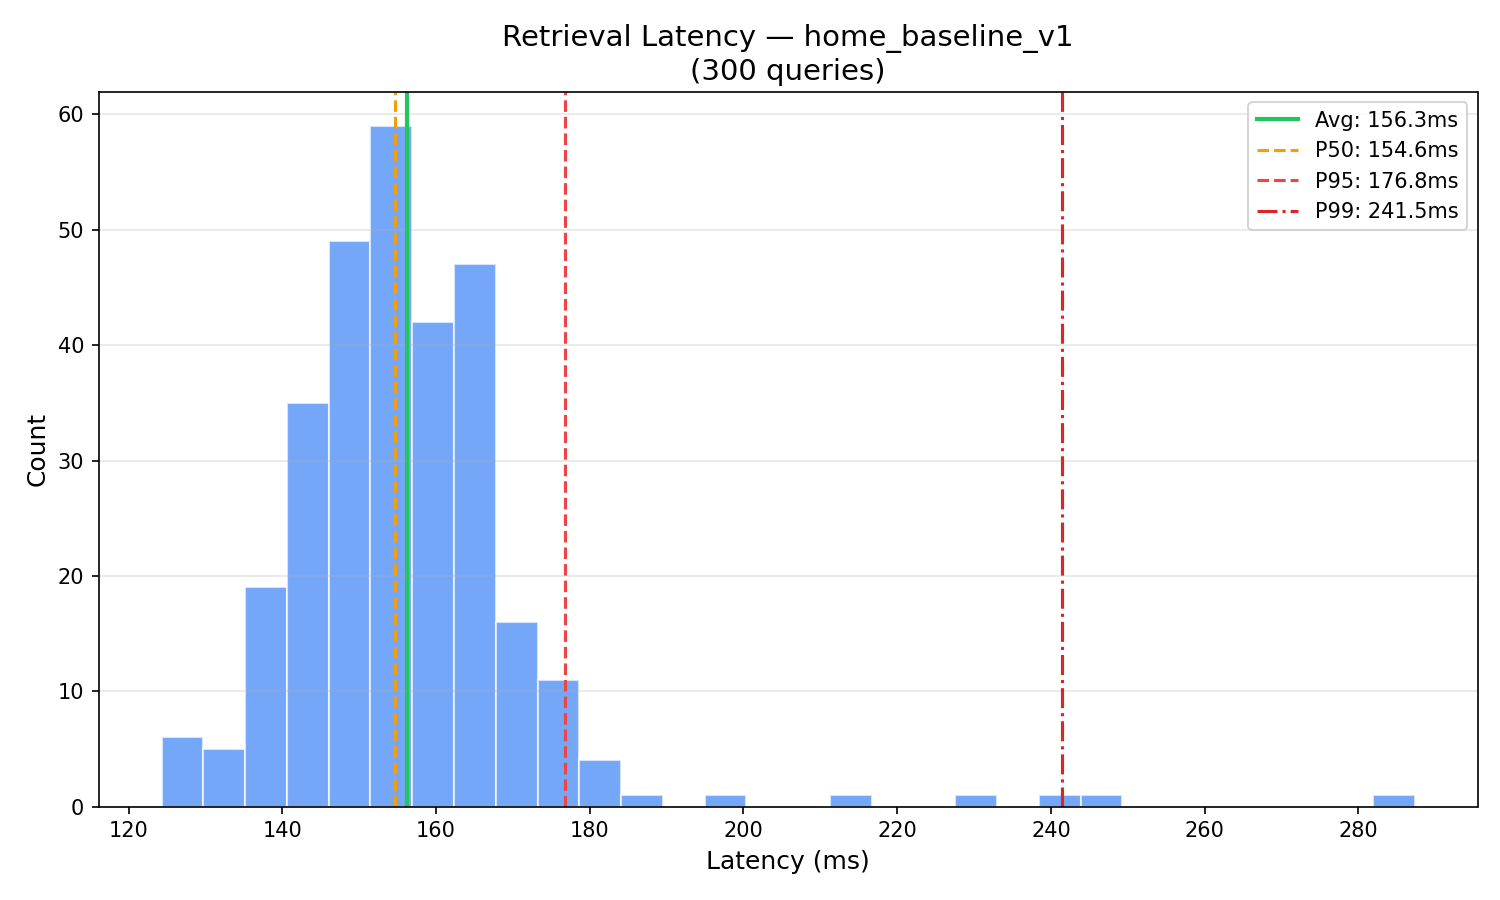
\includegraphics[width=0.92\textwidth]{Images/evaluation/recommender/latency_dist_home_baseline_v1.png}
    \caption{Phân bố độ trễ truy xuất của \texttt{home\_baseline\_v1}}
    \label{fig:appendix_home_latency_dist}
\end{figure}
\end{document}

